\documentclass[11pt]{article}
\usepackage[paperwidth=220mm,paperheight=320mm,left=17.5mm,right=17.5mm,top=20mm,bottom=20mm,headheight=12pt,headsep=12pt,footskip=15pt]{geometry}
\usepackage{fix-cm}
\usepackage{fontspec}
\usepackage{amsmath,amssymb,graphicx}
\usepackage{fancyhdr}
\usepackage[unicode,hidelinks,bookmarksopen=false]{hyperref}
\usepackage{polyglossia}
\setmainlanguage{latin}
\setotherlanguages{arabic,greek}
\setmainfont{Linux Libertine O}[Ligatures=TeX]
\newfontfamily\greekfont{FreeSerif}[Script=Greek]
\newfontfamily\arabicfont{Amiri}[Script=Arabic,Scale=1.0]
\newfontfamily\syriacfont{Noto Sans Syriac}[Script=Syriac,Scale=0.9]
\graphicspath{{../source/presentation/}}
\hypersetup{pdftitle={Nallino: Praefatio, conspectus, addenda et emendanda. S01 v003},pdfauthor={Carlo Alfonso Nallino},pdfsubject={Historical Nallino layer. Source-first transcription candidate; unresolved readings documented separately.}}
\pagestyle{fancy}\fancyhf{}
\newcommand{\leftfolio}{}\newcommand{\rightfolio}{}
\fancyhead[L]{\fontsize{8}{10}\selectfont\leftfolio}
\fancyhead[C]{\fontsize{8}{10}\selectfont\leftmark}
\fancyhead[R]{\fontsize{8}{10}\selectfont\rightfolio}
\fancyfoot[L]{\fontsize{7.5}{9}\selectfont\rightmark}
\fancyfoot[R]{\fontsize{7.5}{9}\selectfont\thepage}
\renewcommand{\headrulewidth}{0.25pt}
\renewcommand{\footrulewidth}{0pt}
\setlength{\parindent}{0pt}\setlength{\parskip}{0pt}
\setlength{\emergencystretch}{0pt}
\newcommand{\asterism}{\raisebox{0.4ex}{\scriptsize *}\kern-0.5em\raisebox{-0.5ex}{\scriptsize **}}
\newcommand{\sourceglyph}[1]{\raisebox{-0.20em}{\includegraphics[height=1.30em]{#1.png}}}
\newsavebox{\sourcelinebox}
\newcommand{\SourceLine}[2]{%
 \sbox{\sourcelinebox}{\strut\hypertarget{#1}{}#2}%
 \ifdim\wd\sourcelinebox>\linewidth\typeout{SOURCEWIDTH|#1|\the\wd\sourcelinebox|\the\linewidth}\fi%
 \noindent\usebox{\sourcelinebox}\par}
\newcommand{\BeginSource}[2]{\clearpage\gdef\leftfolio{}\gdef\rightfolio{}\markboth{#2}{#1}\hypertarget{#1}{}\pdfbookmark[0]{#1}{book-#1}\fontsize{12}{14.8}\selectfont}
\newcommand{\NotesStart}{\par\vspace{7pt}\hrule height0.25pt\vspace{5pt}\fontsize{10}{12.25}\selectfont}
\tracinglostchars=2
\begin{document}


\markboth{ADMONITIO EDITIONIS DIGITALIS}{S01-v003 — MODERN\_EDITORIAL}
\hypertarget{S01-v003-EDITORIAL-NOTICE}{}
\pdfbookmark[0]{Admonitio editionis digitalis}{editorial-notice}
\vspace*{25mm}
\begin{center}
{\fontsize{11}{15}\selectfont\addfontfeatures{LetterSpace=3} CAROLUS ALPHONSUS NALLINO\par}
\vspace{12mm}
{\fontsize{25}{34}\selectfont Praefatio\par Conspectus librorum\par Addenda et emendanda\par}
\vspace{10mm}
{\fontsize{12}{17}\selectfont\itshape Pars prima, 1903\par}
\vspace{18mm}
{\fontsize{10}{14}\selectfont S01 · v003\par}
\end{center}
\vspace{12mm}
\fontsize{11}{16}\selectfont
Haec materia ad Nallini apparatum pertinet, non ad textum Arabicum auctoris.
Loci aliis linguis ab ipso Nallino relati in sua forma servati sunt.\par\medskip
Transcriptio per totum ambitum fontis prima vice recognita est; in hac
versione loci selecti iterum ad imagines fontis collati et errores transcriptionis
emendati sunt, lectionibus prioribus in tabulis servatis.
Lectiones incertae in indice separato recensentur; signa nondum certo expressa
imaginibus fontis servantur. Addenda Nallini describuntur, non tacite locis prioribus inseruntur.\par\medskip
Figura astronomica in ipso fonte mutila est. Quae desunt non sunt restituta;
solae fasciae instrumenti digitalis extrinsecus additae a figura exhibita abscissae sunt.\par\medskip
Recognitio independens omnium verborum nondum facta est.
Textus editabilis, imagines integrae, lectionum rationes, indices locorum et
signaturae SHA-256 in fasciculo huius editionis separatim praebentur.\par\medskip
Fons: exemplar digitale SRC01, paginae 2, 10, 12–89.
Dispositiones omnium paginarum 1–89 in indice continentur.

\BeginSource{AB01-PDF0002}{FIGURA ASTRONOMICA}
\vspace*{25mm}
\begin{center}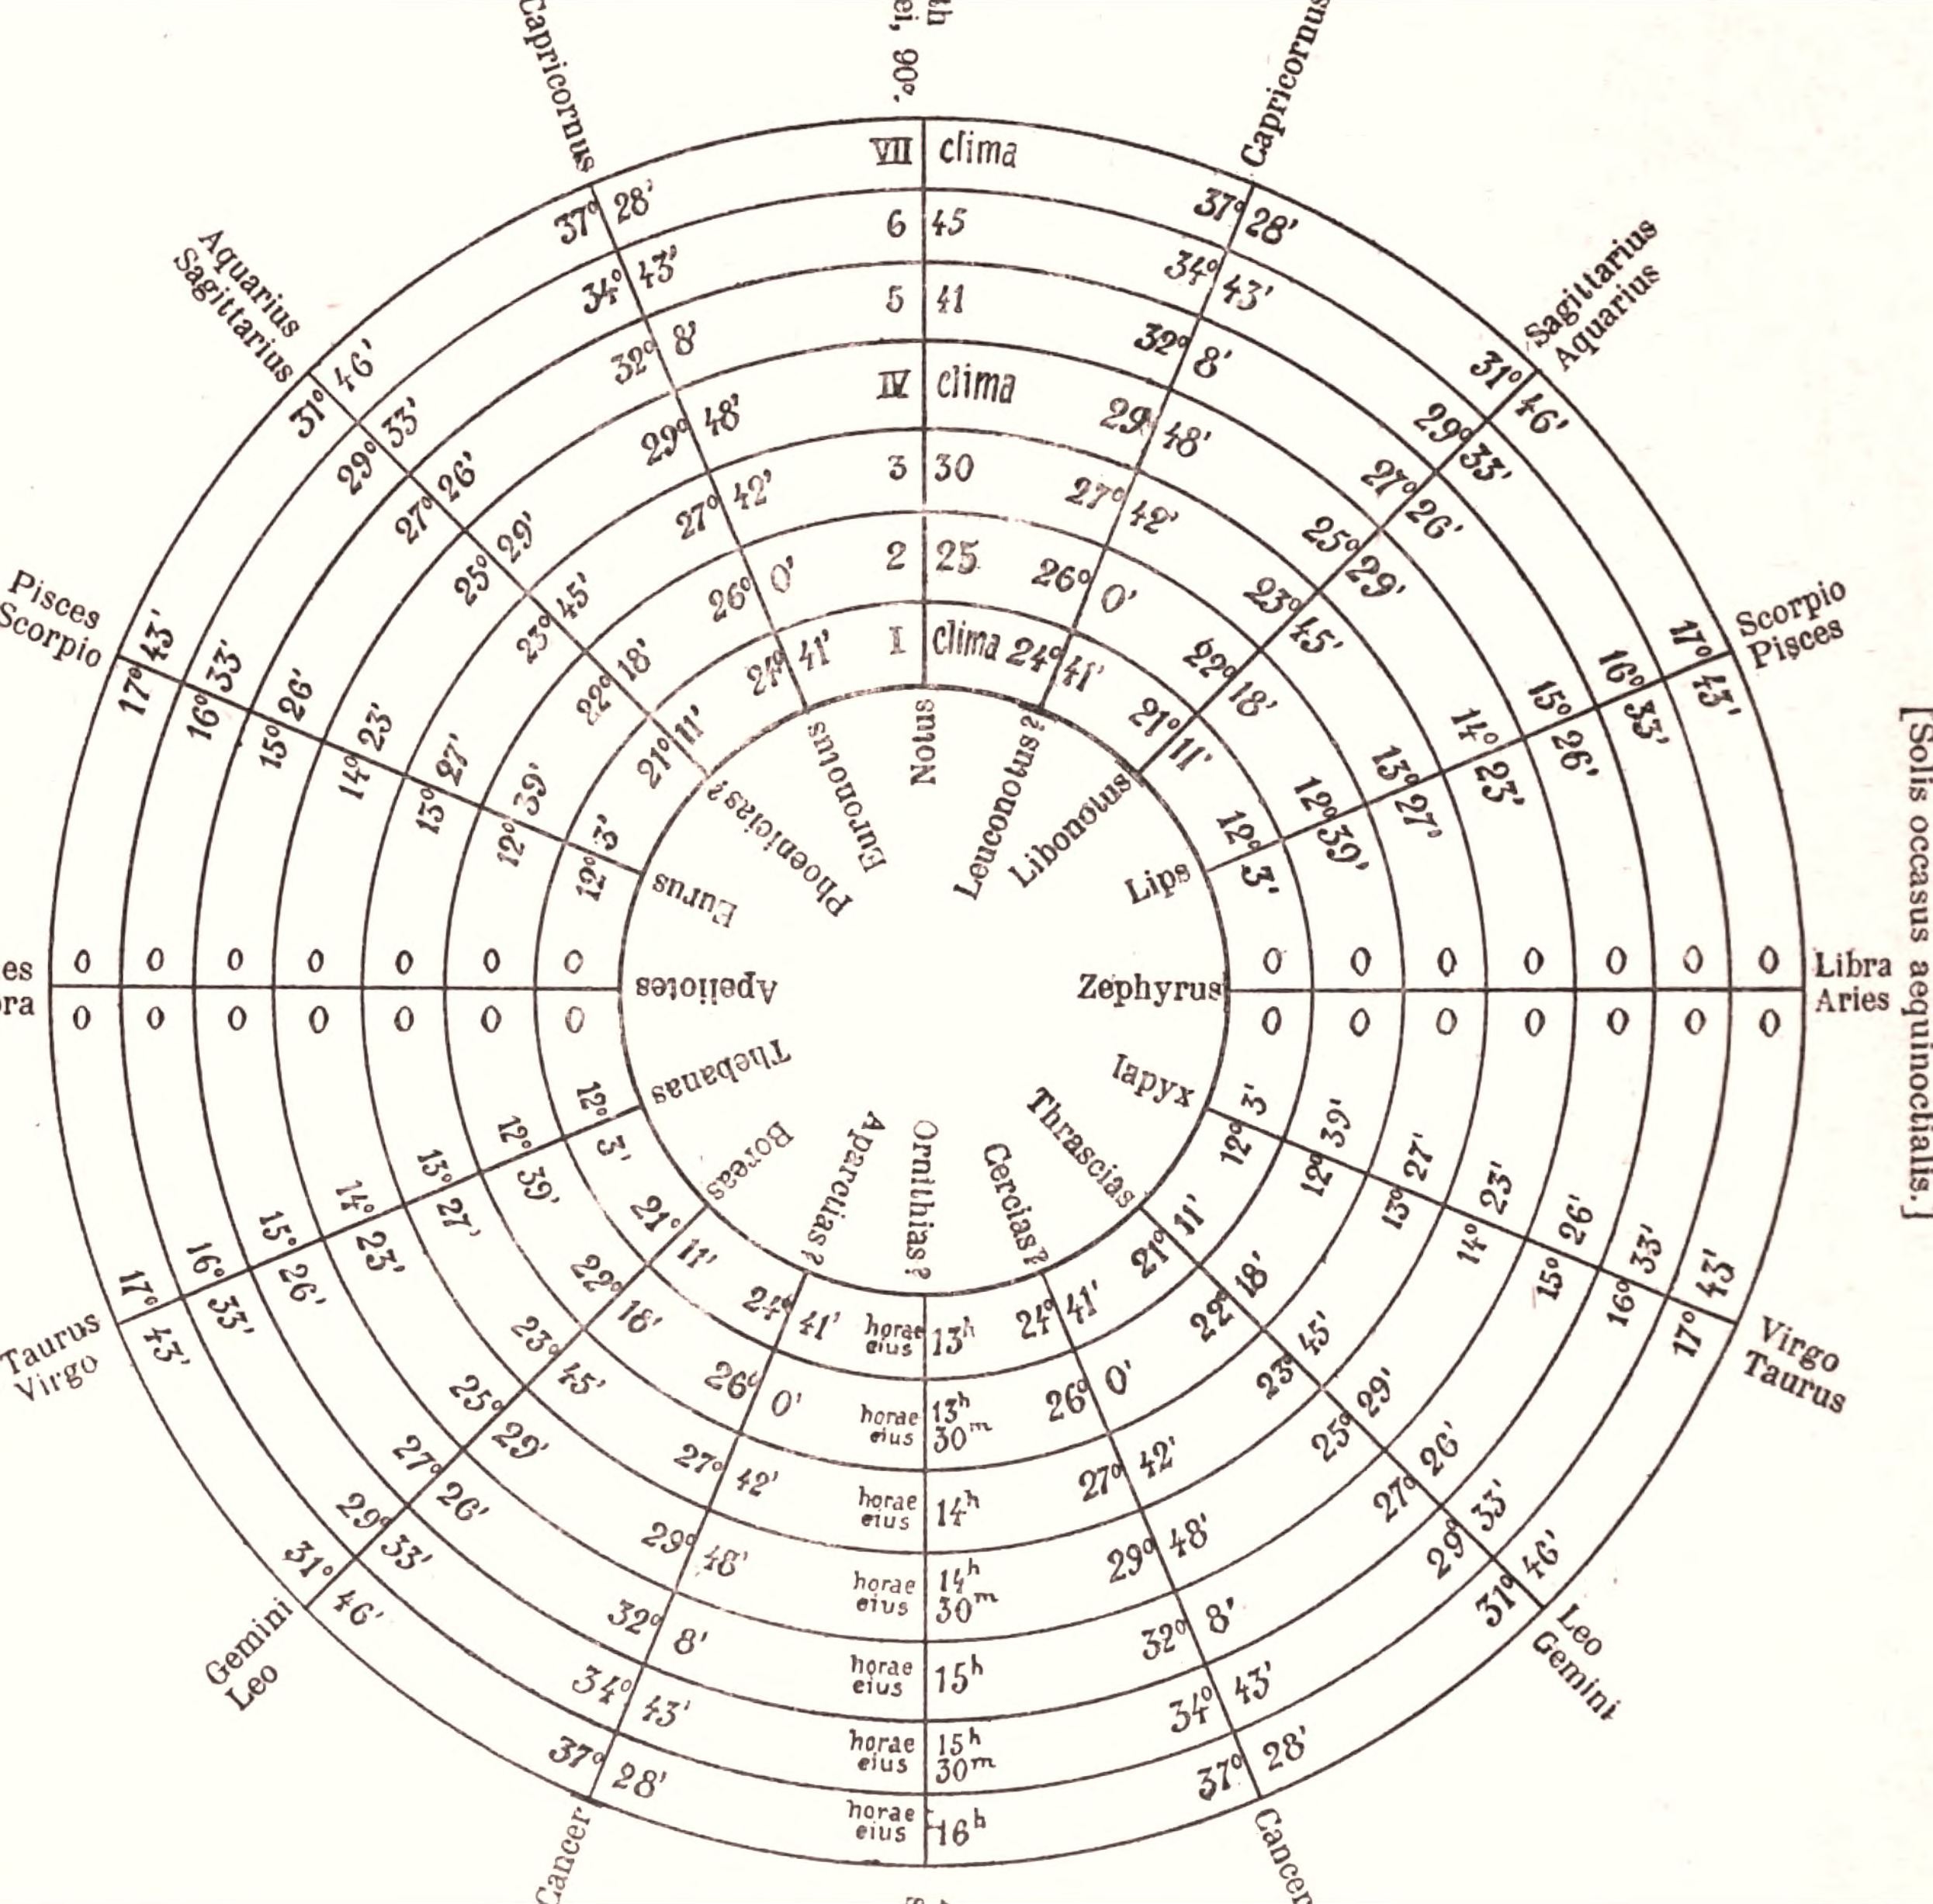
\includegraphics[width=\textwidth]{AB01-PDF0002-F01.png}\end{center}
\BeginSource{AB01-PDF0010}{}
\vspace*{70mm}\begin{center}\fontsize{13}{21}\selectfont
\hypertarget{AB01-PDF0010-body-L001}{}AL-BATTĀNĪ {\small sive} ALBATENII\par
\hypertarget{AB01-PDF0010-body-L002}{}OPUS ASTRONOMICUM\par
\end{center}
\BeginSource{AB01-PDF0012}{}
\begin{center}
{\fontsize{9}{15.299999999999999}\selectfont \hypertarget{AB01-PDF0012-body-L001}{}PUBBLICAZIONI\par}
{\fontsize{9}{15.299999999999999}\selectfont \hypertarget{AB01-PDF0012-body-L002}{}DEL REALE OSSERVATORIO DI BRERA IN MILANO.\par}
{\fontsize{9}{15.299999999999999}\selectfont \hypertarget{AB01-PDF0012-body-L003}{}N. XL. Parte I.\par}
\vspace{15mm}
{\fontsize{13}{22.099999999999998}\selectfont \hypertarget{AB01-PDF0012-body-L004}{}AL-BATTĀNĪ {\small sive} ALBATENII\par}
{\fontsize{21}{35.699999999999996}\selectfont \hypertarget{AB01-PDF0012-body-L005}{}OPUS ASTRONOMICUM.\par}
\vspace{10mm}
{\fontsize{9}{15.299999999999999}\selectfont \hypertarget{AB01-PDF0012-body-L006}{}AD FIDEM CODICIS ESCURIALENSIS ARABICE EDITUM\par}
{\fontsize{9}{15.299999999999999}\selectfont \hypertarget{AB01-PDF0012-body-L007}{}LATINE VERSUM, ADNOTATIONIBUS INSTRUCTUM\par}
{\fontsize{9}{15.299999999999999}\selectfont \hypertarget{AB01-PDF0012-body-L008}{}A\par}
{\fontsize{13}{22.099999999999998}\selectfont \hypertarget{AB01-PDF0012-body-L009}{}CAROLO ALPHONSO NALLINO.\par}
\vspace{25mm}
{\fontsize{13}{22.099999999999998}\selectfont \hypertarget{AB01-PDF0012-body-L010}{}PARS PRIMA\par}
{\fontsize{9}{15.299999999999999}\selectfont \hypertarget{AB01-PDF0012-body-L011}{}VERSIO CAPITUM CUM ANIMADVERSIONIBUS.\par}
\vspace{30mm}
{\fontsize{9}{15.299999999999999}\selectfont \hypertarget{AB01-PDF0012-body-L012}{}MEDIOLANI INSUBRUM\par}
{\fontsize{9}{15.299999999999999}\selectfont \hypertarget{AB01-PDF0012-body-L013}{}PROSTAT APUD ULRICHUM HOEPLIUM\par}
{\fontsize{9}{15.299999999999999}\selectfont \hypertarget{AB01-PDF0012-body-L014}{}REGIUM BIBLIOPOLAM\par}
{\fontsize{9}{15.299999999999999}\selectfont \hypertarget{AB01-PDF0012-body-L015}{}IN XYSTO CHRISTOPHORIANO, NN. 58-63.\par}
{\fontsize{9}{15.299999999999999}\selectfont \hypertarget{AB01-PDF0012-body-L016}{}1903.\par}
\end{center}
\BeginSource{AB01-PDF0013}{}
\vspace*{215mm}\begin{center}\fontsize{9}{12}\selectfont
\hypertarget{AB01-PDF0013-body-L001}{}ROMAE MCMIII. — Excudebat C. DE LUIGI.\par
\end{center}
\BeginSource{AB01-PDF0014}{}
\vspace*{78mm}\begin{center}\fontsize{12}{24}\selectfont
\hypertarget{AB01-PDF0014-body-L001}{}PARENTIBVS MEIS OPTIMIS\par
\hypertarget{AB01-PDF0014-body-L002}{}NVNQVAM SATIS MEMOR ET GRATVS\par
\hypertarget{AB01-PDF0014-body-L003}{}D. D\par
\end{center}
\BeginSource{AB01-PDF0016}{}
\begin{center}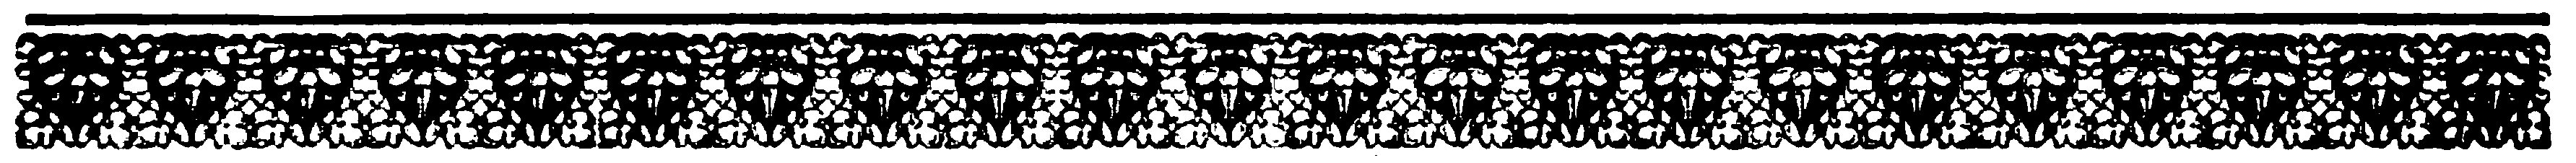
\includegraphics[width=.91\textwidth]{AB01-PDF0016-F01.png}\par\vspace{20mm}{\fontsize{20}{26}\selectfont PRAEFATIO}\end{center}\vspace{17mm}
\begin{minipage}[t]{\textwidth}
% AB01-PDF0016-body-L001
\SourceLine{AB01-PDF0016-body-L001}{§ 1, {\itshape Albatenii vita}: I. de Albatenii vita testes Arabici; II. observationes in testes Arabicos. — § 2, {\itshape Al-}}
% AB01-PDF0016-body-L002
\SourceLine{AB01-PDF0016-body-L002}{{\itshape batenii scripta minora}: I. de ascensionibus inter paxillos; II. de quantitatibus applicationum;}
% AB01-PDF0016-body-L003
\SourceLine{AB01-PDF0016-body-L003}{III. commentarius in Tetrabiblum. — § 3, {\itshape Scripta spuria}: I. Archimedis compendium; II. de}
% AB01-PDF0016-body-L004
\SourceLine{AB01-PDF0016-body-L004}{instrumentis observatoriis; III. Almagesti compendium; IV. commentarius in Centiloquium}
% AB01-PDF0016-body-L005
\SourceLine{AB01-PDF0016-body-L005}{V. de planetis et ascendente; VI. Almagesti parvum; VII. tria opuscula astrologica. — § 4, {\itshape Opus}}
% AB01-PDF0016-body-L006
\SourceLine{AB01-PDF0016-body-L006}{{\itshape astronomicum}: I. operis nomen ac aetas; II. de Albatenio posteri quid senserint; III. nostra de}
% AB01-PDF0016-body-L007
\SourceLine{AB01-PDF0016-body-L007}{opere astronomico sententia; IV. trigonometria Albateniana; V. operis astronomici versiones}
% AB01-PDF0016-body-L008
\SourceLine{AB01-PDF0016-body-L008}{(Latina Roberti Cestrensis, Latina Platonis Tiburtini, Hispanica ignoti auctoris); VI. codices}
% AB01-PDF0016-body-L009
\SourceLine{AB01-PDF0016-body-L009}{Arabici; VII. qua ratione opus Albatenianum ediderim ac Latine verterim. Conclusio.}
% AB01-PDF0016-body-L010
\SourceLine{AB01-PDF0016-body-L010}{}
% AB01-PDF0016-body-L011
\SourceLine{AB01-PDF0016-body-L011}{§ 1. Albatenii vita.}
% AB01-PDF0016-body-L012
\SourceLine{AB01-PDF0016-body-L012}{I. {\itshape De Albatenii vita testes Arabici.} — {\addfontfeatures{LetterSpace=1.0} Albatenii} vitam narraturo etiam hodie non}
% AB01-PDF0016-body-L013
\SourceLine{AB01-PDF0016-body-L013}{alii fere Arabici fontes succurrunt quam quibus {\addfontfeatures{LetterSpace=1.0} D. Chwolsohn} (1) et {\addfontfeatures{LetterSpace=1.0} M. Steinschnei-}}
% AB01-PDF0016-body-L014
\SourceLine{AB01-PDF0016-body-L014}{{\addfontfeatures{LetterSpace=1.0} der} (2) usi sunt; novis tamen subsidiis comparatis, possunt quaedam ab Arabibus tradita rec-}
% AB01-PDF0016-body-L015
\SourceLine{AB01-PDF0016-body-L015}{tius quam duobus illis clarissimis viris contigerit intelligi aut etiam emendari. Albateniana}
% AB01-PDF0016-body-L016
\SourceLine{AB01-PDF0016-body-L016}{autem scripta nobis longe melius et certius nunc cognita sunt.}
\NotesStart
\noindent\begin{minipage}[t]{.485\linewidth}\fontsize{10}{12.25}\selectfont
% AB01-PDF0016-notes_left-L001
\SourceLine{AB01-PDF0016-notes_left-L001}{(1) {\itshape Die Ssabier und der Ssabismus}, St. Peters-}
% AB01-PDF0016-notes_left-L002
\SourceLine{AB01-PDF0016-notes_left-L002}{burg 1856, t. I, p. 611-15.}
% AB01-PDF0016-notes_left-L003
\SourceLine{AB01-PDF0016-notes_left-L003}{(2) {\itshape Vite di matematici arabi tratte da un'o-}}
% AB01-PDF0016-notes_left-L004
\SourceLine{AB01-PDF0016-notes_left-L004}{{\itshape pera inedita di} {\addfontfeatures{LetterSpace=1.0} B. Baldi}, {\itshape con note di} {\addfontfeatures{LetterSpace=1.0} M. Stein-}}
% AB01-PDF0016-notes_left-L005
\SourceLine{AB01-PDF0016-notes_left-L005}{{\addfontfeatures{LetterSpace=1.0} schneider}, in Bullettino di bibliografia e di storia}
% AB01-PDF0016-notes_left-L006
\SourceLine{AB01-PDF0016-notes_left-L006}{delle scienze matematiche e fisiche, t. V, Roma 1872,}
% AB01-PDF0016-notes_left-L007
\SourceLine{AB01-PDF0016-notes_left-L007}{adnot. p. 450-458. Liber bis seorsum etiam editus;}
% AB01-PDF0016-notes_left-L008
\SourceLine{AB01-PDF0016-notes_left-L008}{primum anno 1873 (108 pp.), nulla mutatione facta;}
% AB01-PDF0016-notes_left-L009
\SourceLine{AB01-PDF0016-notes_left-L009}{postea anno 1874 (100 pp.), qua in editione nonnulla}
% AB01-PDF0016-notes_left-L010
\SourceLine{AB01-PDF0016-notes_left-L010}{emendata et omissa, alia addita, perpauca mendose}
% AB01-PDF0016-notes_left-L011
\SourceLine{AB01-PDF0016-notes_left-L011}{impressa sunt. Hanc alteram editionem siglo {\itshape extr.}}
% AB01-PDF0016-notes_left-L012
\SourceLine{AB01-PDF0016-notes_left-L012}{indicabo; notae Steinschneider ad Albatenium per-}
\end{minipage}\hfill\begin{minipage}[t]{.485\linewidth}\fontsize{10}{12.25}\selectfont
% AB01-PDF0016-notes_right-L001
\SourceLine{AB01-PDF0016-notes_right-L001}{tinentes sunt p. 26-31. Ceterum Steinschneider non-}
% AB01-PDF0016-notes_right-L002
\SourceLine{AB01-PDF0016-notes_right-L002}{nisi textum Baldianum illustrare volebat; qua re de}
% AB01-PDF0016-notes_right-L003
\SourceLine{AB01-PDF0016-notes_right-L003}{Albatenio non omnia quae Arabes narraverunt ex-}
% AB01-PDF0016-notes_right-L004
\SourceLine{AB01-PDF0016-notes_right-L004}{posuit. — Brevissime vitam et scripta nostri nar-}
% AB01-PDF0016-notes_right-L005
\SourceLine{AB01-PDF0016-notes_right-L005}{rant {\addfontfeatures{LetterSpace=1.0} C. Brockelmann}, {\itshape Geschichte der Arabi-}}
% AB01-PDF0016-notes_right-L006
\SourceLine{AB01-PDF0016-notes_right-L006}{{\itshape schen Litteratur}, Berlin 1898-1902, t. I, p. 222, atque}
% AB01-PDF0016-notes_right-L007
\SourceLine{AB01-PDF0016-notes_right-L007}{{\addfontfeatures{LetterSpace=1.0} H. Suter}, {\itshape Die Mathematiker und Astronomen}}
% AB01-PDF0016-notes_right-L008
\SourceLine{AB01-PDF0016-notes_right-L008}{{\itshape der Araber und ihre Werke}, Leipzig 1900, p. 45-47,}
% AB01-PDF0016-notes_right-L009
\SourceLine{AB01-PDF0016-notes_right-L009}{nr. 89 (cf. eiusdem {\itshape Nachträge und Berichtigungen},}
% AB01-PDF0016-notes_right-L010
\SourceLine{AB01-PDF0016-notes_right-L010}{in Abhandlungen zur Geschichte der mathematischen}
% AB01-PDF0016-notes_right-L011
\SourceLine{AB01-PDF0016-notes_right-L011}{Wissenschaften, fasc. XIV, Leipzig 1902, p. 164).}
\end{minipage}
\end{minipage}
\BeginSource{AB01-PDF0017}{PRAEFATIO}
\gdef\leftfolio{VIII}
\begin{minipage}[t]{\textwidth}
% AB01-PDF0017-body-L001
\SourceLine{AB01-PDF0017-body-L001}{Duo praesertim Arabum scriptores de Albatenio notitias nobis tradiderunt, {\addfontfeatures{LetterSpace=1.0} an-Nadīm} (1)}
% AB01-PDF0017-body-L002
\SourceLine{AB01-PDF0017-body-L002}{scilicet ac {\addfontfeatures{LetterSpace=1.0} Ibn al-Qifṭī} (2). Haec narrant (3):}
% AB01-PDF0017-body-L003
\SourceLine{AB01-PDF0017-body-L003}{« Abū ‘Abd Allāh Muḥammad ibn Ǵābir ibn Sinān <ar-Raqqī> al-Ḥarrānī, [cognomine]}
% AB01-PDF0017-body-L004
\SourceLine{AB01-PDF0017-body-L004}{« {\addfontfeatures{LetterSpace=1.0} al-Battānī} notus, {\itshape unus illustrium in observandis sideribus [virorum], et principum}}
% AB01-PDF0017-body-L005
\SourceLine{AB01-PDF0017-body-L005}{« {\itshape in scientia geometriae ac astronomiae, in cognitione stellarum, in arte astrologica Est}}
% AB01-PDF0017-body-L006
\SourceLine{AB01-PDF0017-body-L006}{« {\itshape ei insigne opus astronomicum} (4), {\itshape quo Solis et Lunae observationes ab eo factae con-}}
% AB01-PDF0017-body-L007
\SourceLine{AB01-PDF0017-body-L007}{« {\itshape tinentur et emendatio eorum motuum in libro Ptolemaei, qui Almagestum inscribitur,}}
% AB01-PDF0017-body-L008
\SourceLine{AB01-PDF0017-body-L008}{« {\itshape constitutorum. Eo in [opere] motus quinque errantium stellarum, iuxta correctiones}}
% AB01-PDF0017-body-L009
\SourceLine{AB01-PDF0017-body-L009}{« {\itshape quas inferre potuit, exponit simul cum reliquis sphaerae caelestis supputationibus quae}}
% AB01-PDF0017-body-L010
\SourceLine{AB01-PDF0017-body-L010}{« {\itshape opus sunt.}}
% AB01-PDF0017-body-L011
\SourceLine{AB01-PDF0017-body-L011}{« {\itshape Pars eius observationum, quas in opere astronomico memorat, anno 267 heg.} (5)}
% AB01-PDF0017-body-L012
\SourceLine{AB01-PDF0017-body-L012}{« {\itshape fuerunt, pars anno 287} (6). {\itshape Nullus in Islamismo cognoscitur, qui eum in sideribus}}
% AB01-PDF0017-body-L013
\SourceLine{AB01-PDF0017-body-L013}{« {\itshape exacte observandis ac eorum motibus investigandis adaequaverit.} Origine Sabius, ab}
% AB01-PDF0017-body-L014
\SourceLine{AB01-PDF0017-body-L014}{« [urbe] Ḥarrān. Observare coepit, iuxta quae narrat Ǵa‘far ibn al-Muktafī (7), {\itshape ab ipso}}
% AB01-PDF0017-body-L015
\SourceLine{AB01-PDF0017-body-L015}{« {\itshape [Albatenio ea accipiens]} (8), anno 264 (9), usque ad annum 306 (10) {\itshape [pergens]}; stellas fixas}
% AB01-PDF0017-body-L016
\SourceLine{AB01-PDF0017-body-L016}{« in opere astronomico suo ad annum 299 (11) posuit. Venit Baghdād cum [gente vocata] Banū}
% AB01-PDF0017-body-L017
\SourceLine{AB01-PDF0017-body-L017}{« az-Zayyāt, ex incolis [urbis] ar-Raqqah, ut tributa iniuste illis (12) exacta repeteret (13). Inde}
% AB01-PDF0017-body-L018
\SourceLine{AB01-PDF0017-body-L018}{« rediens, in itinere obiit in Qaṣr al-Ǵiṣṣ anno 317 (14). Eius opera haec sunt: Opus astrono-}
\NotesStart
\noindent\begin{minipage}[t]{.485\linewidth}\fontsize{10}{12.25}\selectfont
% AB01-PDF0017-notes_left-L001
\SourceLine{AB01-PDF0017-notes_left-L001}{(1) {\itshape Kitāb al-Fihrist mit Anmerkungen heraus-}}
% AB01-PDF0017-notes_left-L002
\SourceLine{AB01-PDF0017-notes_left-L002}{{\itshape gegeben von} {\addfontfeatures{LetterSpace=1.0} G. Flügel}, Leipzig 1871-1872, t. I,}
% AB01-PDF0017-notes_left-L003
\SourceLine{AB01-PDF0017-notes_left-L003}{p. 279; {\itshape Das Mathematiker-Verzeichniss im Fihrist}}
% AB01-PDF0017-notes_left-L004
\SourceLine{AB01-PDF0017-notes_left-L004}{{\itshape des} {\addfontfeatures{LetterSpace=1.0} an-Nadīm} {\itshape übersetzt von H. Suter}, in Ab-}
% AB01-PDF0017-notes_left-L005
\SourceLine{AB01-PDF0017-notes_left-L005}{handl. z. Gesch. der Mathematik, fasc. VI, Leipzig 1892,}
% AB01-PDF0017-notes_left-L006
\SourceLine{AB01-PDF0017-notes_left-L006}{p. 35. — Scripsit sub finem IV saec. heg.}
% AB01-PDF0017-notes_left-L007
\SourceLine{AB01-PDF0017-notes_left-L007}{(2) In inedita « {\itshape Sapientum historia} »; locus de}
% AB01-PDF0017-notes_left-L008
\SourceLine{AB01-PDF0017-notes_left-L008}{Albatenio Arabice et Latine apud {\addfontfeatures{LetterSpace=1.0} M. Casiri}, {\itshape Bi-}}
% AB01-PDF0017-notes_left-L009
\SourceLine{AB01-PDF0017-notes_left-L009}{{\itshape bliotheca Arabico-Hispana Escurialensis}, Matriti}
% AB01-PDF0017-notes_left-L010
\SourceLine{AB01-PDF0017-notes_left-L010}{1760-70, t. I, p. 344, et, cum aliquot additamentis ex}
% AB01-PDF0017-notes_left-L011
\SourceLine{AB01-PDF0017-notes_left-L011}{operis codicibus Parisiensibus, apud {\addfontfeatures{LetterSpace=1.0} Sédillot} in}
% AB01-PDF0017-notes_left-L012
\SourceLine{AB01-PDF0017-notes_left-L012}{praefatione ad textum {\addfontfeatures{LetterSpace=1.0} Oloug-Beg}, p. xxxi-ii. Con-}
% AB01-PDF0017-notes_left-L013
\SourceLine{AB01-PDF0017-notes_left-L013}{tuli etiam codicem in Bibliotheca Regiae Academiae}
% AB01-PDF0017-notes_left-L014
\SourceLine{AB01-PDF0017-notes_left-L014}{Lyncaeorum Romae asservatum. — Auctor mortuus}
% AB01-PDF0017-notes_left-L015
\SourceLine{AB01-PDF0017-notes_left-L015}{est die 13 ramaḍān 646 (30 Dec. 1248).}
% AB01-PDF0017-notes_left-L016
\SourceLine{AB01-PDF0017-notes_left-L016}{(3) Quae solus {\addfontfeatures{LetterSpace=1.0} Ibn al-Qifṭī} habet Italicis seu}
% AB01-PDF0017-notes_left-L017
\SourceLine{AB01-PDF0017-notes_left-L017}{inclinatis litteris impressa sunt; quae solus {\addfontfeatures{LetterSpace=1.0} an-Na-}}
% AB01-PDF0017-notes_left-L018
\SourceLine{AB01-PDF0017-notes_left-L018}{{\addfontfeatures{LetterSpace=1.0} dīm} uncis fractis < > inclusa; quae ad sensum}
% AB01-PDF0017-notes_left-L019
\SourceLine{AB01-PDF0017-notes_left-L019}{melius declarandum addo uncis quadratis [ ] contenta.}
% AB01-PDF0017-notes_left-L020
\SourceLine{AB01-PDF0017-notes_left-L020}{(4) Arabice {\itshape zīǵ}; cfr. quae in § 4, nr. I dicam,}
% AB01-PDF0017-notes_left-L021
\SourceLine{AB01-PDF0017-notes_left-L021}{de hoc opere agens.}
% AB01-PDF0017-notes_left-L022
\SourceLine{AB01-PDF0017-notes_left-L022}{(5) Perperam {\addfontfeatures{LetterSpace=1.0} Ibn al-Qifṭī} 269, quia in}
% AB01-PDF0017-notes_left-L023
\SourceLine{AB01-PDF0017-notes_left-L023}{fonte \textarabic{\upshape تسعة} « novem » loco \textarabic{\upshape سبعة} « septem » invene-}
% AB01-PDF0017-notes_left-L024
\SourceLine{AB01-PDF0017-notes_left-L024}{rat. Error in Arabica scriptura facillimus et frequen-}
% AB01-PDF0017-notes_left-L025
\SourceLine{AB01-PDF0017-notes_left-L025}{tissimus. — Annus 267 heg. incepit die 11 Aug. 880}
% AB01-PDF0017-notes_left-L026
\SourceLine{AB01-PDF0017-notes_left-L026}{Chr., iuxta {\itshape Arabicorum astronomorum} usum, quem}
% AB01-PDF0017-notes_left-L027
\SourceLine{AB01-PDF0017-notes_left-L027}{semper in indicando initio annorum hegirae sequor.}
% AB01-PDF0017-notes_left-L028
\SourceLine{AB01-PDF0017-notes_left-L028}{Iuxta usum civilem, die 12 Augusti.}
% AB01-PDF0017-notes_left-L029
\SourceLine{AB01-PDF0017-notes_left-L029}{(6) Inc. 6 Ian. 900.}
\end{minipage}\hfill\begin{minipage}[t]{.485\linewidth}\fontsize{10}{12.25}\selectfont
% AB01-PDF0017-notes_right-L001
\SourceLine{AB01-PDF0017-notes_right-L001}{(7) {\addfontfeatures{LetterSpace=1.0} Abū ’l-faḍl Ǵa‘far Ibn al-Muktafī},}
% AB01-PDF0017-notes_right-L002
\SourceLine{AB01-PDF0017-notes_right-L002}{khalifae al-Muktafī (289-295 heg.) filius, valde in}
% AB01-PDF0017-notes_right-L003
\SourceLine{AB01-PDF0017-notes_right-L003}{multis scientiis et in veterum recentiorumque sa-}
% AB01-PDF0017-notes_right-L004
\SourceLine{AB01-PDF0017-notes_right-L004}{pientum historia versatus. Natus anno 294 (inc.}
% AB01-PDF0017-notes_right-L005
\SourceLine{AB01-PDF0017-notes_right-L005}{21 Oct. 906), mortuus mense ṣafar 377 (Iunio 987);}
% AB01-PDF0017-notes_right-L006
\SourceLine{AB01-PDF0017-notes_right-L006}{iuvenis admodum igitur erat cum Albatenium inter-}
% AB01-PDF0017-notes_right-L007
\SourceLine{AB01-PDF0017-notes_right-L007}{rogabat. Unus ex an-Nadīm fontibus ({\itshape Kitāb al-Fih-}}
% AB01-PDF0017-notes_right-L008
\SourceLine{AB01-PDF0017-notes_right-L008}{{\itshape rist}, p. 16, 275, 269). De eo {\addfontfeatures{LetterSpace=1.0} Suter}, {\itshape Die Mathema-}}
% AB01-PDF0017-notes_right-L009
\SourceLine{AB01-PDF0017-notes_right-L009}{{\itshape tiker}, p. 64-65, nr. 142; {\addfontfeatures{LetterSpace=1.0} Ibn al-Qifṭī} apud {\addfontfeatures{LetterSpace=1.0} Ca-}}
% AB01-PDF0017-notes_right-L010
\SourceLine{AB01-PDF0017-notes_right-L010}{{\addfontfeatures{LetterSpace=1.0} siri} I, 422 et {\addfontfeatures{LetterSpace=1.0} Sédillot} p. xiv et xlvi-vii; {\addfontfeatures{LetterSpace=1.0} Abū}}
% AB01-PDF0017-notes_right-L011
\SourceLine{AB01-PDF0017-notes_right-L011}{{\addfontfeatures{LetterSpace=1.0} ’l-faraǵ}, {\itshape Ta’rīkh ad-duwal} edit. Ṣālḥānī, Bey-}
% AB01-PDF0017-notes_right-L012
\SourceLine{AB01-PDF0017-notes_right-L012}{rūt 1890, p. 306-307.}
% AB01-PDF0017-notes_right-L013
\SourceLine{AB01-PDF0017-notes_right-L013}{(8) \textarabic{\upshape عن لسانه}. Pro his {\addfontfeatures{LetterSpace=1.0} an-Nadīm}: « dicens se}
% AB01-PDF0017-notes_right-L014
\SourceLine{AB01-PDF0017-notes_right-L014}{« illum interrogavisse, eumque respondisse quod in-}
% AB01-PDF0017-notes_right-L015
\SourceLine{AB01-PDF0017-notes_right-L015}{« ceperat..... ».}
% AB01-PDF0017-notes_right-L016
\SourceLine{AB01-PDF0017-notes_right-L016}{(9) Inc. 12 Sept. 877.}
% AB01-PDF0017-notes_right-L017
\SourceLine{AB01-PDF0017-notes_right-L017}{(10) Inc. 13 Iunii 918.}
% AB01-PDF0017-notes_right-L018
\SourceLine{AB01-PDF0017-notes_right-L018}{(11) Falsum pro 267, ut in adnotationibus ad}
% AB01-PDF0017-notes_right-L019
\SourceLine{AB01-PDF0017-notes_right-L019}{II tomum ostendam. Error in scriptura Arabica non}
% AB01-PDF0017-notes_right-L020
\SourceLine{AB01-PDF0017-notes_right-L020}{difficilis: \textarabic{\upshape تسعة وتسعين} pro \textarabic{\upshape سبعة وستين}.}
% AB01-PDF0017-notes_right-L021
\SourceLine{AB01-PDF0017-notes_right-L021}{(12) An hoc pronomine al-Battānī quoque desi-}
% AB01-PDF0017-notes_right-L022
\SourceLine{AB01-PDF0017-notes_right-L022}{gnetur, e textu Arabico (\textarabic{\upshape لهم}) non liquet.}
% AB01-PDF0017-notes_right-L023
\SourceLine{AB01-PDF0017-notes_right-L023}{(13) Arabice \textarabic{\upshape وورد الى بغداد..... في ظلامات كانت لهم},}
% AB01-PDF0017-notes_right-L024
\SourceLine{AB01-PDF0017-notes_right-L024}{a nostratibus non recte intellectum ({\addfontfeatures{LetterSpace=1.0} Casiri}: « le-}
% AB01-PDF0017-notes_right-L025
\SourceLine{AB01-PDF0017-notes_right-L025}{« ctica vectus »!). Cfr. {\addfontfeatures{LetterSpace=1.0} Dozy}, {\itshape Supplément aux di-}}
% AB01-PDF0017-notes_right-L026
\SourceLine{AB01-PDF0017-notes_right-L026}{{\itshape ctionn. arabes} II, 291, s. v. \textarabic{\upshape ظلم}; de peculiari sensu}
% AB01-PDF0017-notes_right-L027
\SourceLine{AB01-PDF0017-notes_right-L027}{vocis \textarabic{\upshape مَظْلَمَة} vel \textarabic{\upshape ظُلامَة} vide {\itshape Glossarium ad Anna-}}
% AB01-PDF0017-notes_right-L028
\SourceLine{AB01-PDF0017-notes_right-L028}{{\itshape les} {\addfontfeatures{LetterSpace=1.0} aṭ-Ṭabarī}, p. cccxlii, s. v. \textarabic{\upshape ظلم}.}
% AB01-PDF0017-notes_right-L029
\SourceLine{AB01-PDF0017-notes_right-L029}{(14) Inc. 13 Febr. 929.}
\end{minipage}
\end{minipage}
\BeginSource{AB01-PDF0018}{PRAEFATIO}
\gdef\rightfolio{IX}
\begin{minipage}[t]{\textwidth}
% AB01-PDF0018-body-L001
\SourceLine{AB01-PDF0018-body-L001}{« micum in duabus editionibus, <priore et altera; altera priore melior>. — Liber <cogni-}
% AB01-PDF0018-body-L002
\SourceLine{AB01-PDF0018-body-L002}{« tionis> ascensionum signorum <in spatiis inter quartas sphaerae caelestis>. — {\itshape Liber} (1)}
% AB01-PDF0018-body-L003
\SourceLine{AB01-PDF0018-body-L003}{« <verificationis> quantitatum applicationum; eum pro Abū ’l-ḥasan Ibn al-Furāt compo-}
% AB01-PDF0018-body-L004
\SourceLine{AB01-PDF0018-body-L004}{« suit (2). — {\itshape Liber Commentarii in Tetrabiblum Ptolemaei} » (3).}
% AB01-PDF0018-body-L005
\SourceLine{AB01-PDF0018-body-L005}{Quae solus Ibn al-Qifṭī habet, ab historia universali {\itshape at-ta‘rīf bi ṭabaqāt al-umam} in-}
% AB01-PDF0018-body-L006
\SourceLine{AB01-PDF0018-body-L006}{scripta, cuius auctor {\addfontfeatures{LetterSpace=1.0} Ṣā‘id al-Andalusī} (4), provenire existimo; verba enim ab « insigne}
% AB01-PDF0018-body-L007
\SourceLine{AB01-PDF0018-body-L007}{opus astronomicum » usque ad « sphaerae caelestis supputationibus » refert {\addfontfeatures{LetterSpace=1.0} Ḥāǵǵī Khalī-}}
% AB01-PDF0018-body-L008
\SourceLine{AB01-PDF0018-body-L008}{{\addfontfeatures{LetterSpace=1.0} fah} ex illo Ṣā‘idi opere (5).}
% AB01-PDF0018-body-L009
\SourceLine{AB01-PDF0018-body-L009}{A libro illius an-Nadīm originem ducit Albatenii vita, quam in lexicon suum biographicum}
% AB01-PDF0018-body-L010
\SourceLine{AB01-PDF0018-body-L010}{recepit {\addfontfeatures{LetterSpace=1.0} Ibn Khallikān} (6): « Abū ‘Abd Allāh Muḥammad ibn Ǵābir ibn Sinān, Ḥarrānensis}
% AB01-PDF0018-body-L011
\SourceLine{AB01-PDF0018-body-L011}{« origine, {\itshape incola ar-Raqqah} (7), al-Battānī, calculator et astronomus praeclarus, auctor operis}
% AB01-PDF0018-body-L012
\SourceLine{AB01-PDF0018-body-L012}{« astronomici Sabii [appellati]. Sunt ei admirabiles operationes, observationesque accuratissime}
% AB01-PDF0018-body-L013
\SourceLine{AB01-PDF0018-body-L013}{« perfectae. Observare anno 264 coepit, usque ad annum 306 [pergens]; stellas fixas in opere}
% AB01-PDF0018-body-L014
\SourceLine{AB01-PDF0018-body-L014}{« astronomico suo ad annum 299 posuit. Unicus aetatis suae in arte sua; operationes eius}
% AB01-PDF0018-body-L015
\SourceLine{AB01-PDF0018-body-L015}{« magnam eius excellentiam vastamque doctrinam indicant. Obiit anno 317, a Baghdād rediens,}
% AB01-PDF0018-body-L016
\SourceLine{AB01-PDF0018-body-L016}{« loco Qaṣr al-Ḥaḍr (8) appellato. Eum islamiticam fidem amplexum esse non comperi; sed}
% AB01-PDF0018-body-L017
\SourceLine{AB01-PDF0018-body-L017}{« nomen eius [Muḥammad] eum Muslimum factum esse indicat. Eius scripta haec sunt: Opus}
% AB01-PDF0018-body-L018
\SourceLine{AB01-PDF0018-body-L018}{« astronomicum, in duabus editionibus, prior et altera; altera melior. — Liber cognitionis}
% AB01-PDF0018-body-L019
\SourceLine{AB01-PDF0018-body-L019}{« ascensionum signorum in spatiis inter quartas sphaerae caelestis. — Epistula de {\itshape quantitate}}
% AB01-PDF0018-body-L020
\SourceLine{AB01-PDF0018-body-L020}{« {\itshape applicationum. — Liber quo explanarit} (9) {\itshape quatuor quartas sphaerae caelestis. — Epi-}}
% AB01-PDF0018-body-L021
\SourceLine{AB01-PDF0018-body-L021}{« {\itshape stula de} (10) verificatione quantitatum applicationum. — Commentarius Tetrabibli Ptolemaei.}
\NotesStart
\noindent\begin{minipage}[t]{.485\linewidth}\fontsize{10}{12.25}\selectfont
% AB01-PDF0018-notes_left-L001
\SourceLine{AB01-PDF0018-notes_left-L001}{(1) {\addfontfeatures{LetterSpace=1.0} An-Nadīm}: « Et nota est eius epistula... ».}
% AB01-PDF0018-notes_left-L002
\SourceLine{AB01-PDF0018-notes_left-L002}{At postea miro modo \textarabic{\upshape عمل} « {\itshape eum} composuit », ut}
% AB01-PDF0018-notes_left-L003
\SourceLine{AB01-PDF0018-notes_left-L003}{apud {\addfontfeatures{LetterSpace=1.0} Ibn al-Qifṭī}, loco \textarabic{\upshape عملها} « eam composuit ».}
% AB01-PDF0018-notes_left-L004
\SourceLine{AB01-PDF0018-notes_left-L004}{Error negligentia ortus in fonte transcribendo, cu-}
% AB01-PDF0018-notes_left-L005
\SourceLine{AB01-PDF0018-notes_left-L005}{ius \textarabic{\upshape كتاب} « librum » antea in \textarabic{\upshape رسالة} « epistulam » mu-}
% AB01-PDF0018-notes_left-L006
\SourceLine{AB01-PDF0018-notes_left-L006}{taverat. Ergo quae {\addfontfeatures{LetterSpace=1.0} Steinschneider} et {\addfontfeatures{LetterSpace=1.0} Suter}}
% AB01-PDF0018-notes_left-L007
\SourceLine{AB01-PDF0018-notes_left-L007}{coniecerunt respuenda sunt, ut in § 2, nr. II, os-}
% AB01-PDF0018-notes_left-L008
\SourceLine{AB01-PDF0018-notes_left-L008}{tendam.}
% AB01-PDF0018-notes_left-L009
\SourceLine{AB01-PDF0018-notes_left-L009}{(2) Verba « eum pro etc. » desunt in textu}
% AB01-PDF0018-notes_left-L010
\SourceLine{AB01-PDF0018-notes_left-L010}{{\addfontfeatures{LetterSpace=1.0} Ibn al-Qifṭī} apud {\addfontfeatures{LetterSpace=1.0} Casiri}, sed in codicibus}
% AB01-PDF0018-notes_left-L011
\SourceLine{AB01-PDF0018-notes_left-L011}{Parisiensibus (apud {\addfontfeatures{LetterSpace=1.0} Sédillot}) et Lyncaeorum ex-}
% AB01-PDF0018-notes_left-L012
\SourceLine{AB01-PDF0018-notes_left-L012}{stant.}
% AB01-PDF0018-notes_left-L013
\SourceLine{AB01-PDF0018-notes_left-L013}{(3) Deest apud {\addfontfeatures{LetterSpace=1.0} an-Nadīm}, qui tamen alio}
% AB01-PDF0018-notes_left-L014
\SourceLine{AB01-PDF0018-notes_left-L014}{loco (p. 268, in vers. {\addfontfeatures{LetterSpace=1.0} Suter} p. 20) al-Battānī iis}
% AB01-PDF0018-notes_left-L015
\SourceLine{AB01-PDF0018-notes_left-L015}{qui Tetrabiblum explicaverint adnumerat.}
% AB01-PDF0018-notes_left-L016
\SourceLine{AB01-PDF0018-notes_left-L016}{(4) Almeriae, in Hispania, natus anno 420 heg.}
% AB01-PDF0018-notes_left-L017
\SourceLine{AB01-PDF0018-notes_left-L017}{(inc. 19 Ian. 1029); iudex Toleti, qua in urbe die 4}
% AB01-PDF0018-notes_left-L018
\SourceLine{AB01-PDF0018-notes_left-L018}{shawwāl 462 (16 Iul. 1070) obiit. Illius operis per-}
% AB01-PDF0018-notes_left-L019
\SourceLine{AB01-PDF0018-notes_left-L019}{pauca fragmenta supersunt.}
% AB01-PDF0018-notes_left-L020
\SourceLine{AB01-PDF0018-notes_left-L020}{(5) {\addfontfeatures{LetterSpace=1.0} Ḥāǵī Khalfae} {\itshape Lexicon bibliographi-}}
% AB01-PDF0018-notes_left-L021
\SourceLine{AB01-PDF0018-notes_left-L021}{{\itshape cum et encyclopaedicum, primum edidit, Latine}}
% AB01-PDF0018-notes_left-L022
\SourceLine{AB01-PDF0018-notes_left-L022}{{\itshape vertit et commentario indicibusque instruxit G. Flü-}}
% AB01-PDF0018-notes_left-L023
\SourceLine{AB01-PDF0018-notes_left-L023}{{\itshape gel}, Leipzig-London 1835-58, t. III, p. 568, nr. 6961.}
% AB01-PDF0018-notes_left-L024
\SourceLine{AB01-PDF0018-notes_left-L024}{Ibi pro \textarabic{\upshape المثبتة} « constitutorum » minus bene \textarabic{\upshape المبينة}}
% AB01-PDF0018-notes_left-L025
\SourceLine{AB01-PDF0018-notes_left-L025}{« explanatorum »; falso autem \textarabic{\upshape وإصلاحه حركاته} loco}
\end{minipage}\hfill\begin{minipage}[t]{.485\linewidth}\fontsize{10}{12.25}\selectfont
% AB01-PDF0018-notes_right-L001
\SourceLine{AB01-PDF0018-notes_right-L001}{\textarabic{\upshape وإصلاحه لحركاتها} (Ibn al-Qifṭī \textarabic{\upshape وإصلاح حركاتها}). — {\addfontfeatures{LetterSpace=1.0} Ṣā‘id}}
% AB01-PDF0018-notes_right-L002
\SourceLine{AB01-PDF0018-notes_right-L002}{in opere suo Albatenium memoravisse testatur etiam}
% AB01-PDF0018-notes_right-L003
\SourceLine{AB01-PDF0018-notes_right-L003}{nota ad unum codicum Vindobonensium Ibn al-Qifṭī,}
% AB01-PDF0018-notes_right-L004
\SourceLine{AB01-PDF0018-notes_right-L004}{apud {\addfontfeatures{LetterSpace=1.0} Chwolsohn} I, 611, adn. 1.}
% AB01-PDF0018-notes_right-L005
\SourceLine{AB01-PDF0018-notes_right-L005}{(6) {\addfontfeatures{LetterSpace=1.0} Ibn Challikan}, {\itshape Vitae illustrium vi-}}
% AB01-PDF0018-notes_right-L006
\SourceLine{AB01-PDF0018-notes_right-L006}{{\itshape rorum, edidit F. Wüstenfeld}, Gottingae 1835-42,}
% AB01-PDF0018-notes_right-L007
\SourceLine{AB01-PDF0018-notes_right-L007}{nr. 719; {\itshape Wafāyāt al-a‘yān}, Kahirae, typogr. al-}
% AB01-PDF0018-notes_right-L008
\SourceLine{AB01-PDF0018-notes_right-L008}{-Waṭan, 1299 heg., t. II, p. 506-508; {\addfontfeatures{LetterSpace=1.0} Ibn Khalli-}}
% AB01-PDF0018-notes_right-L009
\SourceLine{AB01-PDF0018-notes_right-L009}{{\addfontfeatures{LetterSpace=1.0} kan’s} {\itshape biographical dictionary translated by Mac}}
% AB01-PDF0018-notes_right-L010
\SourceLine{AB01-PDF0018-notes_right-L010}{{\itshape Guckin de Slane}, Paris-London 1843-71, t. IV,}
% AB01-PDF0018-notes_right-L011
\SourceLine{AB01-PDF0018-notes_right-L011}{p. 317-20. — Auctor obiit Damasci die 26 raǵab 681}
% AB01-PDF0018-notes_right-L012
\SourceLine{AB01-PDF0018-notes_right-L012}{(30 Oct. 1282).}
% AB01-PDF0018-notes_right-L013
\SourceLine{AB01-PDF0018-notes_right-L013}{(7) Haec in editione dumtaxat Wüstenfeldiana}
% AB01-PDF0018-notes_right-L014
\SourceLine{AB01-PDF0018-notes_right-L014}{sunt.}
% AB01-PDF0018-notes_right-L015
\SourceLine{AB01-PDF0018-notes_right-L015}{(8) Al-Ḥaḍr \textarabic{\upshape الحضر} corruptelam esse exemplaris}
% AB01-PDF0018-notes_right-L016
\SourceLine{AB01-PDF0018-notes_right-L016}{quo Ibn Khallikān usus est, loco veri nominis, \textarabic{\upshape الجص}}
% AB01-PDF0018-notes_right-L017
\SourceLine{AB01-PDF0018-notes_right-L017}{al-Ǵiṣṣ, sub finem § 1 ostendam.}
% AB01-PDF0018-notes_right-L018
\SourceLine{AB01-PDF0018-notes_right-L018}{(9) Ita ed. Wüstenfeld et versio Anglica De}
% AB01-PDF0018-notes_right-L019
\SourceLine{AB01-PDF0018-notes_right-L019}{Slane. Editiones in Aegypto impressae \textarabic{\upshape فيه} omittunt,}
% AB01-PDF0018-notes_right-L020
\SourceLine{AB01-PDF0018-notes_right-L020}{qua re sensus fit: « Liber commentarii quatuor quar-}
% AB01-PDF0018-notes_right-L021
\SourceLine{AB01-PDF0018-notes_right-L021}{tarum ..... ».}
% AB01-PDF0018-notes_right-L022
\SourceLine{AB01-PDF0018-notes_right-L022}{(10) Verba Italicis seu inclinatis litteris impressa,}
% AB01-PDF0018-notes_right-L023
\SourceLine{AB01-PDF0018-notes_right-L023}{in omnibus editionibus exstant; sed manifeste e dit-}
% AB01-PDF0018-notes_right-L024
\SourceLine{AB01-PDF0018-notes_right-L024}{tographia in codice quem Ibn Khallikān prae ma-}
% AB01-PDF0018-notes_right-L025
\SourceLine{AB01-PDF0018-notes_right-L025}{nibus habuit, orta sunt. Quod evidentius e textu Ara-}
\end{minipage}
\end{minipage}
\par\vspace{6pt}\hfill{\fontsize{8}{10}\selectfont 2*}
\BeginSource{AB01-PDF0019}{PRAEFATIO}
\gdef\leftfolio{X}
\begin{minipage}[t]{\textwidth}
% AB01-PDF0019-body-L001
\SourceLine{AB01-PDF0019-body-L001}{« Et alia [scripta]. [Nomen] al-Battānī vocalem {\itshape a} habet post litteram {\itshape B}; [at] Abū Muḥam-}
% AB01-PDF0019-body-L002
\SourceLine{AB01-PDF0019-body-L002}{« mad Hibat Allāh Ibn al-Akfānī (1) vocalem {\itshape i} esse affirmat. Est nomen a B..ttān derivatum,}
% AB01-PDF0019-body-L003
\SourceLine{AB01-PDF0019-body-L003}{« pago (\textarabic{\upshape ناحية}) agri (\textarabic{\upshape من أعمال}) Ḥarrānensis (2) ..... In alia historia legi eum Baghdād intrasse, po-}
% AB01-PDF0019-body-L004
\SourceLine{AB01-PDF0019-body-L004}{« stea ab ea profectum esse, ac in itinere, anno supra memorato, in Qaṣr al-Ǵiṣṣ (3) obiisse.}
% AB01-PDF0019-body-L005
\SourceLine{AB01-PDF0019-body-L005}{« Dicit Yāqūt al-Ḥamawī in libro suo al-mushtarik inscripto: Qaṣr al-Ǵiṣṣ, prope Sāmarrā, e}
% AB01-PDF0019-body-L006
\SourceLine{AB01-PDF0019-body-L006}{« palatiis ab al-Mu‘taṣim exstructis. — Deus altissimus [omnia] melius scit ».}
% AB01-PDF0019-body-L007
\SourceLine{AB01-PDF0019-body-L007}{{\addfontfeatures{LetterSpace=1.0} Abū ’l-fidā’}, praeclarus historiae et geographiae scriptor qui die 23 muḥarram 732}
% AB01-PDF0019-body-L008
\SourceLine{AB01-PDF0019-body-L008}{(26 Oct. 1331) summum diem obiit, in {\itshape Annalibus}, s. a. 317, Ibn Khallikān sequitur, sed opus}
% AB01-PDF0019-body-L009
\SourceLine{AB01-PDF0019-body-L009}{astronomicum ipse in manibus habuisse videtur (4): « Hoc anno [317] mortuus est Muḥam-}
% AB01-PDF0019-body-L010
\SourceLine{AB01-PDF0019-body-L010}{« mad ibn Ǵābir ibn Sinān, Ḥarrānensis origine, al-Battānī, calculator et astronomus prae-}
% AB01-PDF0019-body-L011
\SourceLine{AB01-PDF0019-body-L011}{« clarus, auctor operis astronomici Sabii [appellati]. {\itshape Nomen eius eum Muslimum factum}}
% AB01-PDF0019-body-L012
\SourceLine{AB01-PDF0019-body-L012}{« {\itshape esse indicat; item eius praefatio in opus astronomicum. Dicit Ibn Khallikān: Eum isla-}}
% AB01-PDF0019-body-L013
\SourceLine{AB01-PDF0019-body-L013}{« {\itshape miticam fidem amplexum esse non comperi.} Sunt ei observationes accuratissime perfe-}
% AB01-PDF0019-body-L014
\SourceLine{AB01-PDF0019-body-L014}{« ctae. Observare anno 264 coepit, usque ad annum 306 [pergens]; stellas fixas in opere}
% AB01-PDF0019-body-L015
\SourceLine{AB01-PDF0019-body-L015}{« astronomico suo ad annum 299 posuit. Eius opus astronomicum in duabus est editionibus,}
% AB01-PDF0019-body-L016
\SourceLine{AB01-PDF0019-body-L016}{« prior et altera; altera melior. Al-Battānī, cum {\itshape a} post {\itshape B} (vel cum {\itshape i}, ut ab aliis dicitur)}
% AB01-PDF0019-body-L017
\SourceLine{AB01-PDF0019-body-L017}{« est nomen a B..ttān derivatum, qui est pagus agri Ḥarrānensis ».}
% AB01-PDF0019-body-L018
\SourceLine{AB01-PDF0019-body-L018}{Nullius momenti et ex Ibn al-Qifṭī hausta sunt quae {\addfontfeatures{LetterSpace=1.0} Abū ’l-faraǵ} (Barhebraeus) in}
% AB01-PDF0019-body-L019
\SourceLine{AB01-PDF0019-body-L019}{{\itshape historia dynastiarum} narrat (5): « Anno 317 mortuus est Muḥammad ibn Ǵābir ibn Sinān}
% AB01-PDF0019-body-L020
\SourceLine{AB01-PDF0019-body-L020}{« Abū ‘Abd Allāh al-Battānī, e praeclaris viris in observatione stellarum. Nullus in Islamismo}
% AB01-PDF0019-body-L021
\SourceLine{AB01-PDF0019-body-L021}{« cognoscitur qui eius excellentiam in sideribus exacte observandis ac eorum motibus investi-}
% AB01-PDF0019-body-L022
\SourceLine{AB01-PDF0019-body-L022}{« gandis assecutus sit. Origine Sabius, ab [urbe] Ḥarrān ».}
% AB01-PDF0019-body-L023
\SourceLine{AB01-PDF0019-body-L023}{Demum {\addfontfeatures{LetterSpace=1.0} al-‘Aynī}, qui Kahirae die 4 dhū ’l-ḥiǵǵah 855 (28 Dec. 1451) obiit, in chro-}
% AB01-PDF0019-body-L024
\SourceLine{AB01-PDF0019-body-L024}{nico inedito {\itshape ‘iqd al-ǵumān}, omnia fere Ibn Khallikāni verba, teste {\addfontfeatures{LetterSpace=1.0} Chwolsohn} I, 615,}
% AB01-PDF0019-body-L025
\SourceLine{AB01-PDF0019-body-L025}{transcripsit.}
% AB01-PDF0019-body-L026
\SourceLine{AB01-PDF0019-body-L026}{Auctores omnes hucusque commemorati ab unico vetere fonte manare videntur. Diver-}
% AB01-PDF0019-body-L027
\SourceLine{AB01-PDF0019-body-L027}{sam originem fortasse habent alii duo, qui tamen nihil fere novi dicunt; scilicet Ẓahīr ad-dīn}
\NotesStart
\noindent\begin{minipage}[t]{.485\linewidth}\fontsize{10}{12.25}\selectfont
% AB01-PDF0019-notes_left-L001
\SourceLine{AB01-PDF0019-notes_left-L001}{bico elucet, ubi verba delenda uncis includo: \textarabic{\upshape وكتاب}}
% AB01-PDF0019-notes_left-L002
\SourceLine{AB01-PDF0019-notes_left-L002}{\textarabic{\upshape معرفة مطالع البروج فيما بين أرباع الفلك ورسالة في [مقدار}}
% AB01-PDF0019-notes_left-L003
\SourceLine{AB01-PDF0019-notes_left-L003}{\textarabic{\upshape الاتصالات وكتاب شرح فيه أربعة أرباع الفلك ورسالة في]}}
% AB01-PDF0019-notes_left-L004
\SourceLine{AB01-PDF0019-notes_left-L004}{\textarabic{\upshape تحقيق أقدار الاتصالات وشرح أربع مقالات بطليموس}.}
% AB01-PDF0019-notes_left-L005
\SourceLine{AB01-PDF0019-notes_left-L005}{(1) Quem De Slane, ad fidem auctoris libri {\itshape an-}}
% AB01-PDF0019-notes_left-L006
\SourceLine{AB01-PDF0019-notes_left-L006}{{\itshape Nuǵūm}, anno 523 (inc. 24 Dec. 1128) mortuum dicit.}
% AB01-PDF0019-notes_left-L007
\SourceLine{AB01-PDF0019-notes_left-L007}{(2) Sequuntur nonnulla de vetustissimi oppidi}
% AB01-PDF0019-notes_left-L008
\SourceLine{AB01-PDF0019-notes_left-L008}{al-Ḥaḍr historia.}
% AB01-PDF0019-notes_left-L009
\SourceLine{AB01-PDF0019-notes_left-L009}{(3) Editiones omnes et versio De Slane hic et}
% AB01-PDF0019-notes_left-L010
\SourceLine{AB01-PDF0019-notes_left-L010}{infra Qaṣr al-Ḥaḍr ut antea. Sed manifeste illis « {\itshape in}}
% AB01-PDF0019-notes_left-L011
\SourceLine{AB01-PDF0019-notes_left-L011}{« {\itshape alia historia legi} ..... » auctor notitias de Alba-}
% AB01-PDF0019-notes_left-L012
\SourceLine{AB01-PDF0019-notes_left-L012}{tenio a praecedentibus discrepantes se etiam me-}
% AB01-PDF0019-notes_left-L013
\SourceLine{AB01-PDF0019-notes_left-L013}{moratas invenisse significare volebat; quod sane non}
% AB01-PDF0019-notes_left-L014
\SourceLine{AB01-PDF0019-notes_left-L014}{fit si iterum Qaṣr al-Ḥaḍr legitur. Omnem dubita-}
% AB01-PDF0019-notes_left-L015
\SourceLine{AB01-PDF0019-notes_left-L015}{tionem dirimit locus {\addfontfeatures{LetterSpace=1.0} Yāqūt} statim infra ab auc-}
% AB01-PDF0019-notes_left-L016
\SourceLine{AB01-PDF0019-notes_left-L016}{tore allatus, qui re vera exstat in opere: {\addfontfeatures{LetterSpace=1.0} Jacut’s}}
% AB01-PDF0019-notes_left-L017
\SourceLine{AB01-PDF0019-notes_left-L017}{{\itshape Moschtarik, das ist Lexicon geographischer Homo-}}
\end{minipage}\hfill\begin{minipage}[t]{.485\linewidth}\fontsize{10}{12.25}\selectfont
% AB01-PDF0019-notes_right-L001
\SourceLine{AB01-PDF0019-notes_right-L001}{{\itshape nyme, herausgegeben von F. Wüstenfeld}, Göttin-}
% AB01-PDF0019-notes_right-L002
\SourceLine{AB01-PDF0019-notes_right-L002}{gen 1846, p. 348. — Celeber geographus Yāqūt die}
% AB01-PDF0019-notes_right-L003
\SourceLine{AB01-PDF0019-notes_right-L003}{20 ramaḍān 626 obiit (12 Aug. 1229).}
% AB01-PDF0019-notes_right-L004
\SourceLine{AB01-PDF0019-notes_right-L004}{(4) Edit. Constantinopolitanae, anno 1286 heg.}
% AB01-PDF0019-notes_right-L005
\SourceLine{AB01-PDF0019-notes_right-L005}{impressae, t. II, p. 79; quam mihi benevolentissime}
% AB01-PDF0019-notes_right-L006
\SourceLine{AB01-PDF0019-notes_right-L006}{C. Schiaparelli suppeditavit. In editione Reiskiana}
% AB01-PDF0019-notes_right-L007
\SourceLine{AB01-PDF0019-notes_right-L007}{({\addfontfeatures{LetterSpace=1.0} Abulfedae} {\itshape Annales Muslemici, Arabice et La-}}
% AB01-PDF0019-notes_right-L008
\SourceLine{AB01-PDF0019-notes_right-L008}{{\itshape tine opera et studiis J. J. Reiskii}, Hafniae 1784-94,}
% AB01-PDF0019-notes_right-L009
\SourceLine{AB01-PDF0019-notes_right-L009}{t. II, p. 358) verba Italicis litteris impressa (\textarabic{\upshape واسمه}}
% AB01-PDF0019-notes_right-L010
\SourceLine{AB01-PDF0019-notes_right-L010}{\textarabic{\upshape يدلّ على إسلامه وكذلك خطبته في زيجه قال ابن خلّكان ولم}}
% AB01-PDF0019-notes_right-L011
\SourceLine{AB01-PDF0019-notes_right-L011}{\textarabic{\upshape اعلم انه اسلم و}) desiderantur; sed exstant quoque in}
% AB01-PDF0019-notes_right-L012
\SourceLine{AB01-PDF0019-notes_right-L012}{codice Annalium in Bibliotheca Nationali Augustae}
% AB01-PDF0019-notes_right-L013
\SourceLine{AB01-PDF0019-notes_right-L013}{Taurinorum asservato (nr. 57 Catalogi mei), quem}
% AB01-PDF0019-notes_right-L014
\SourceLine{AB01-PDF0019-notes_right-L014}{rogatu meo humanissime I. Pizzi inspexit.}
% AB01-PDF0019-notes_right-L015
\SourceLine{AB01-PDF0019-notes_right-L015}{(5) Ed. Ṣālḥānī p. 274. — Auctor mortuus est}
% AB01-PDF0019-notes_right-L016
\SourceLine{AB01-PDF0019-notes_right-L016}{in urbe Marāghah, prope lacum Ūrmiyah, die 6 ǵu-}
% AB01-PDF0019-notes_right-L017
\SourceLine{AB01-PDF0019-notes_right-L017}{mādā II 685 (30 Iul. 1286).}
\end{minipage}
\end{minipage}
\BeginSource{AB01-PDF0020}{PRAEFATIO}
\gdef\rightfolio{XI}
\begin{minipage}[t]{\textwidth}
% AB01-PDF0020-body-L001
\SourceLine{AB01-PDF0020-body-L001}{{\addfontfeatures{LetterSpace=1.0} ‘Alī ibn Abī ’l-Qāsim al-Bayhaqī}, in {\itshape ta’rīkh ḥukamā’ al-islām} « historia sapientum Isla-}
% AB01-PDF0020-body-L002
\SourceLine{AB01-PDF0020-body-L002}{mismi (1) » paulo post 553 heg. (inc. 1 Febr. 1158) scripta, et, saeculo VII heg. (XIII Chr.),}
% AB01-PDF0020-body-L003
\SourceLine{AB01-PDF0020-body-L003}{{\addfontfeatures{LetterSpace=1.0} Muḥammad ibn Maḥmūd ash-Shahrazūrī} in {\itshape Nuzhat al-arwāḥ wa rawḍat al-ifrāḥ}}
% AB01-PDF0020-body-L004
\SourceLine{AB01-PDF0020-body-L004}{« animorum delectamentum et oblectationis horti (2) ». Ambo inedita; de Albatenio locos, quos}
% AB01-PDF0020-body-L005
\SourceLine{AB01-PDF0020-body-L005}{in illis esse deprehenderam e magno Catalogo Ahlwardtiano codicum Arabicorum Berolinensium,}
% AB01-PDF0020-body-L006
\SourceLine{AB01-PDF0020-body-L006}{Dr. Eugenius {\addfontfeatures{LetterSpace=1.0} Mittwoch} libentissime in usum meum transcripsit. Quae solus ‘Alī al-Bayhaqī}
% AB01-PDF0020-body-L007
\SourceLine{AB01-PDF0020-body-L007}{habet, in textu uncis fractis < > includo, in versione litteris Italicis imprimo; vocales a me,}
% AB01-PDF0020-body-L008
\SourceLine{AB01-PDF0020-body-L008}{non a codicibus proveniunt: \textarabic{\upshape محمد بن جابر البتاني <هو محمد بن جابر بن سنان بن ثابت بن قرة الحراني> صاحب}}
% AB01-PDF0020-body-L009
\SourceLine{AB01-PDF0020-body-L009}{\textarabic{\upshape الرصد المشهور بعد أيام المأمون وكان <حكيماً> عارفاً بتفاصيل أجزاء} (3) \textarabic{\upshape علوم الحكمة وقد انفق أموالاً في الرصد وبتّان قرية}}
% AB01-PDF0020-body-L010
\SourceLine{AB01-PDF0020-body-L010}{\textarabic{\upshape <في حدود} (4) \textarabic{\upshape > حرّان واليها يُنْسَب <محمد بن جابر} (5) \textarabic{\upshape وما نُقِل عنه كُدُورة العمر في جار السّوء والولد العاقّ}}
% AB01-PDF0020-body-L011
\SourceLine{AB01-PDF0020-body-L011}{\textarabic{\upshape والمرأة السّيّئة الأخلاق وقال أشياء لا يُسْتَقَلّ قليلها الدَّيْن والعداوة والمرض>} « Muḥammad Ibn Ǵābir al-Battānī,}
% AB01-PDF0020-body-L012
\SourceLine{AB01-PDF0020-body-L012}{« {\itshape scilicet Muḥammad ibn Ǵābir ibn Sinān ibn Thābit ibn Qurrah al-Ḥarrānī} (6), domi-}
% AB01-PDF0020-body-L013
\SourceLine{AB01-PDF0020-body-L013}{« nus speculae (7) celeberrimae, post aetatem al-Ma’mūn. Erat {\itshape sapiens}, in subtiliter distin-}
% AB01-PDF0020-body-L014
\SourceLine{AB01-PDF0020-body-L014}{« guendo partes disciplinarum philosophiae (8) versatus. Divitias impendit in speculam. Battān}
% AB01-PDF0020-body-L015
\SourceLine{AB01-PDF0020-body-L015}{« vicus est {\itshape in finibus} (9) Ḥarrān; ab eo nomen relativum {\itshape Muḥammad ibn Ǵābir} (10) accepit.}
% AB01-PDF0020-body-L016
\SourceLine{AB01-PDF0020-body-L016}{« {\itshape Ex iis quae [tanquam] ab illo [dicta] feruntur: Vitae afflictio est in filio non obe-}}
% AB01-PDF0020-body-L017
\SourceLine{AB01-PDF0020-body-L017}{« {\itshape dienti et vicino pravo et muliere malis moribus praedita. Dixit} [{\itshape etiam}]: {\itshape Sunt res qua-}}
% AB01-PDF0020-body-L018
\SourceLine{AB01-PDF0020-body-L018}{« {\itshape rum parva quantitas nunquam pauca censetur; debita pecunia, inimicitia, morbus} ».}
% AB01-PDF0020-body-L019
\SourceLine{AB01-PDF0020-body-L019}{Utrum hae sententiae ab al-Battānī proveniant, an potius ‘Alī al-Bayhaqī, ut in initio vitae,}
% AB01-PDF0020-body-L020
\SourceLine{AB01-PDF0020-body-L020}{nostrum cum alio viro confuderit, iudicare non audeo.}
% AB01-PDF0020-body-L021
\SourceLine{AB01-PDF0020-body-L021}{II. {\itshape Observationes in testes Arabicos.} — Restat ut Arabica haec testimonia illustremus,}
% AB01-PDF0020-body-L022
\SourceLine{AB01-PDF0020-body-L022}{emendationes etiam et additamenta illis interdum inferentes.}
% AB01-PDF0020-body-L023
\SourceLine{AB01-PDF0020-body-L023}{Pauca de nominibus propriis Arabicis praemittenda sunt (11). Apud Muslimos parentes li-}
% AB01-PDF0020-body-L024
\SourceLine{AB01-PDF0020-body-L024}{beris {\itshape nomina} seu {\itshape praenomina (ism)} imponunt, quorum numerus exiguus; vix centum attin-}
\NotesStart
\noindent\begin{minipage}[t]{.485\linewidth}\fontsize{10}{12.25}\selectfont
% AB01-PDF0020-notes_left-L001
\SourceLine{AB01-PDF0020-notes_left-L001}{(1) Fol. 9,v.-10,r. codicis Berolinensis ({\addfontfeatures{LetterSpace=1.0} Ahl-}}
% AB01-PDF0020-notes_left-L002
\SourceLine{AB01-PDF0020-notes_left-L002}{{\addfontfeatures{LetterSpace=1.0} wardt}, {\itshape Verzeichniss}, t. IX, p. 457, nr. 10052).}
% AB01-PDF0020-notes_left-L003
\SourceLine{AB01-PDF0020-notes_left-L003}{(2) Fol. 146,r.-v. cod. Berolinensis ({\addfontfeatures{LetterSpace=1.0} Ahlwardt}}
% AB01-PDF0020-notes_left-L004
\SourceLine{AB01-PDF0020-notes_left-L004}{IX, 459, nr. 10055).}
% AB01-PDF0020-notes_left-L005
\SourceLine{AB01-PDF0020-notes_left-L005}{(3) Al-Bayhaqī \textarabic{\upshape اجراء}.}
% AB01-PDF0020-notes_left-L006
\SourceLine{AB01-PDF0020-notes_left-L006}{(4) Pro his ash-Shahrazūrī \textarabic{\upshape من قرى}.}
% AB01-PDF0020-notes_left-L007
\SourceLine{AB01-PDF0020-notes_left-L007}{(5) Pro his ash-Shahr. \textarabic{\upshape الشيخ الفاضل}; reliqua}
% AB01-PDF0020-notes_left-L008
\SourceLine{AB01-PDF0020-notes_left-L008}{non habet.}
% AB01-PDF0020-notes_left-L009
\SourceLine{AB01-PDF0020-notes_left-L009}{(6) Al-Bayhaqī manifeste Sinān avum Albate-}
% AB01-PDF0020-notes_left-L010
\SourceLine{AB01-PDF0020-notes_left-L010}{nii confundit cum Sinān filio Thābit ibn Qurrah, me-}
% AB01-PDF0020-notes_left-L011
\SourceLine{AB01-PDF0020-notes_left-L011}{dico, astronomo et mathematico, qui 14 annos post}
% AB01-PDF0020-notes_left-L012
\SourceLine{AB01-PDF0020-notes_left-L012}{Albatenium obiit!}
% AB01-PDF0020-notes_left-L013
\SourceLine{AB01-PDF0020-notes_left-L013}{(7) Hoc sensu \textarabic{\upshape رَصَد} usurpari satis colligitur e}
% AB01-PDF0020-notes_left-L014
\SourceLine{AB01-PDF0020-notes_left-L014}{locis a {\addfontfeatures{LetterSpace=1.0} Dozy}, {\itshape Supplément aux dictionn. arabes},}
% AB01-PDF0020-notes_left-L015
\SourceLine{AB01-PDF0020-notes_left-L015}{I, 533,{\itshape a} laudatis, {\addfontfeatures{LetterSpace=1.0} al-Kutubī}, {\itshape Fawāt al-wafayāt},}
% AB01-PDF0020-notes_left-L016
\SourceLine{AB01-PDF0020-notes_left-L016}{ed. altera, Būlāq 1299 heg., t. II, p. 151 (in vita Na-}
% AB01-PDF0020-notes_left-L017
\SourceLine{AB01-PDF0020-notes_left-L017}{ṣīr ad-dīn, ubi pro \textarabic{\upshape برجيس} et \textarabic{\upshape البناني} restituantur}
% AB01-PDF0020-notes_left-L018
\SourceLine{AB01-PDF0020-notes_left-L018}{\textarabic{\upshape ابرخس} et \textarabic{\upshape البتاني}), et {\addfontfeatures{LetterSpace=1.0} Ḥāǵǵī Khalīfah} III, p. 465-}
% AB01-PDF0020-notes_left-L019
\SourceLine{AB01-PDF0020-notes_left-L019}{-70, nr. 6460 sqq.}
% AB01-PDF0020-notes_left-L020
\SourceLine{AB01-PDF0020-notes_left-L020}{(8) {\itshape Al-ḥikmah} est philosophia sensu latissimo,}
% AB01-PDF0020-notes_left-L021
\SourceLine{AB01-PDF0020-notes_left-L021}{speculativa nempe et naturalis; cfr. {\addfontfeatures{LetterSpace=1.0} Ali Dschor-}}
\end{minipage}\hfill\begin{minipage}[t]{.485\linewidth}\fontsize{10}{12.25}\selectfont
% AB01-PDF0020-notes_right-L001
\SourceLine{AB01-PDF0020-notes_right-L001}{{\addfontfeatures{LetterSpace=1.0} dschani}, {\itshape Definitiones, ed. G. Flügel}, Lipsiae 1845,}
% AB01-PDF0020-notes_right-L002
\SourceLine{AB01-PDF0020-notes_right-L002}{p. 96; {\addfontfeatures{LetterSpace=1.0} at-Tahānawī}, {\itshape Kashf iṣṭilāḥāt al-funūn},}
% AB01-PDF0020-notes_right-L003
\SourceLine{AB01-PDF0020-notes_right-L003}{Constantinopoli 1317 heg. sqq., introductionis p. 41-}
% AB01-PDF0020-notes_right-L004
\SourceLine{AB01-PDF0020-notes_right-L004}{-47. Scientiarum autem {\itshape partes} sunt earum obiectum}
% AB01-PDF0020-notes_right-L005
\SourceLine{AB01-PDF0020-notes_right-L005}{({\itshape mawḍū‘}), quaestiones singulae ({\itshape masā’il}), principia}
% AB01-PDF0020-notes_right-L006
\SourceLine{AB01-PDF0020-notes_right-L006}{fundamentalia ({\itshape mabādi’}); vide {\addfontfeatures{LetterSpace=1.0} at-Tahānawī}, in-}
% AB01-PDF0020-notes_right-L007
\SourceLine{AB01-PDF0020-notes_right-L007}{trod. p. 8-14.}
% AB01-PDF0020-notes_right-L008
\SourceLine{AB01-PDF0020-notes_right-L008}{(9) Ash-Shahrazūrī: « e vicis ».}
% AB01-PDF0020-notes_right-L009
\SourceLine{AB01-PDF0020-notes_right-L009}{(10) Ash-Shahrazūrī: « insignis vir ». Sequentia}
% AB01-PDF0020-notes_right-L010
\SourceLine{AB01-PDF0020-notes_right-L010}{non habet.}
% AB01-PDF0020-notes_right-L011
\SourceLine{AB01-PDF0020-notes_right-L011}{(11) Materies nec parva nec facilis; nobis neces-}
% AB01-PDF0020-notes_right-L012
\SourceLine{AB01-PDF0020-notes_right-L012}{saria dumtaxat expono. Vide {\addfontfeatures{LetterSpace=1.0} Garcin de Tassy},}
% AB01-PDF0020-notes_right-L013
\SourceLine{AB01-PDF0020-notes_right-L013}{{\itshape Mémoires sur les noms propres et les titres mu-}}
% AB01-PDF0020-notes_right-L014
\SourceLine{AB01-PDF0020-notes_right-L014}{{\itshape sulmans}, in Journal Asiatique, ser. V, t. 3, 1854,}
% AB01-PDF0020-notes_right-L015
\SourceLine{AB01-PDF0020-notes_right-L015}{p. 422-510 (multis additionibus auctus anno 1878}
% AB01-PDF0020-notes_right-L016
\SourceLine{AB01-PDF0020-notes_right-L016}{iterum Parisiis impressus); {\addfontfeatures{LetterSpace=1.0} T. E. Colebrooke},}
% AB01-PDF0020-notes_right-L017
\SourceLine{AB01-PDF0020-notes_right-L017}{{\itshape On the proper names of the Muhammadans}, in}
% AB01-PDF0020-notes_right-L018
\SourceLine{AB01-PDF0020-notes_right-L018}{Journal of the R. Asiatic Society, New Series, t. XI,}
% AB01-PDF0020-notes_right-L019
\SourceLine{AB01-PDF0020-notes_right-L019}{1879, p. 171-237; item Arabica commentaria in li-}
% AB01-PDF0020-notes_right-L020
\SourceLine{AB01-PDF0020-notes_right-L020}{brum grammaticum {\itshape Alfiyyah}, cap. \textarabic{\upshape العَلَم}.}
\end{minipage}
\end{minipage}
\BeginSource{AB01-PDF0021}{PRAEFATIO}
\gdef\leftfolio{XII}
\begin{minipage}[t]{\textwidth}
% AB01-PDF0021-body-L001
\SourceLine{AB01-PDF0021-body-L001}{gunt quae frequentius usurpantur. Cognomina, seu familiarum nomina, omnino fere desunt,}
% AB01-PDF0021-body-L002
\SourceLine{AB01-PDF0021-body-L002}{pro quibus solet {\itshape nomen patris}, saepe etiam avi, proavi, abavi etc. indicari. Ita in nostro astro-}
% AB01-PDF0021-body-L003
\SourceLine{AB01-PDF0021-body-L003}{nomo: Muḥammad (quod praenomen est) filius ({\itshape ibn}) Ǵābir filii Sinān. Praeterea adultis non}
% AB01-PDF0021-body-L004
\SourceLine{AB01-PDF0021-body-L004}{raro additur quod Arabes {\itshape kunyah} appellant, seu nomen voce {\itshape Abū} « pater » compositum (1);}
% AB01-PDF0021-body-L005
\SourceLine{AB01-PDF0021-body-L005}{ita in nostro: Abū ‘Abd Allāh « pater Abdallae », probabiliter quia primus eius filius nomen}
% AB01-PDF0021-body-L006
\SourceLine{AB01-PDF0021-body-L006}{‘Abd Allāh habuit (2). Adhibentur demum quoque {\itshape nomina relativa (nisbah)}, a nominibus}
% AB01-PDF0021-body-L007
\SourceLine{AB01-PDF0021-body-L007}{regionum, urbium, tribuum, artium etc. tanquam gentilicia vel patronymica vel possessiva}
% AB01-PDF0021-body-L008
\SourceLine{AB01-PDF0021-body-L008}{ducta; suffixo {\itshape —ī}, rarius {\itshape —ānī, —āwī}, formantur. Ita in nostro, al-Ḥarrānī virum indicat}
% AB01-PDF0021-body-L009
\SourceLine{AB01-PDF0021-body-L009}{ab urbe Ḥarrān oriundum, aut in ea natum, aut eam incolentem; similiter ar-Raqqī hominem}
% AB01-PDF0021-body-L010
\SourceLine{AB01-PDF0021-body-L010}{ad urbem ar-Raqqah quolibet modo pertinentem designat. Complures {\itshape nisbah} unus vir sumere}
% AB01-PDF0021-body-L011
\SourceLine{AB01-PDF0021-body-L011}{potest, ut nostro evenit (al-Ḥarrānī, ar-Raqqī, al-Battānī, aṣ-Ṣābi’). Interdum patris nisbah,}
% AB01-PDF0021-body-L012
\SourceLine{AB01-PDF0021-body-L012}{sibi non bene convenientem, filius etiam accipit.}
% AB01-PDF0021-body-L013
\SourceLine{AB01-PDF0021-body-L013}{Nomen relativum, seu nisbah, al-Battānī a scriptoribus priorum quinque saeculorum he-}
% AB01-PDF0021-body-L014
\SourceLine{AB01-PDF0021-body-L014}{girae explicatum non invenio. Sexto saeculo {\addfontfeatures{LetterSpace=1.0} Ibn al-Akfānī}, sacrarum traditionum cognitione}
% AB01-PDF0021-body-L015
\SourceLine{AB01-PDF0021-body-L015}{praestantissimus vir ({\itshape muḥaddith}), nomen esse al-Bittānī efferendum, contra vulgatam lectio-}
% AB01-PDF0021-body-L016
\SourceLine{AB01-PDF0021-body-L016}{nem, affirmat (3); sed unde petitum nescio an etiam docuerit. — Eodem saeculo {\addfontfeatures{LetterSpace=1.0} as-Sam‘ānī} (4),}
% AB01-PDF0021-body-L017
\SourceLine{AB01-PDF0021-body-L017}{in celeberrimo sed adhuc inedito nominum relativorum lexico, al-Battānī non memorat, sicut}
% AB01-PDF0021-body-L018
\SourceLine{AB01-PDF0021-body-L018}{clar. vir {\addfontfeatures{LetterSpace=1.0} de Rosen} me docet, qui, rogatu meo, codicem Petropolitanum lexici humanissime}
% AB01-PDF0021-body-L019
\SourceLine{AB01-PDF0021-body-L019}{pervolvit.}
% AB01-PDF0021-body-L020
\SourceLine{AB01-PDF0021-body-L020}{At inde ab eiusdem VI saeculi heg. medietate non desunt qui Battānī nomen a pago quo-}
% AB01-PDF0021-body-L021
\SourceLine{AB01-PDF0021-body-L021}{dam {\itshape Battān}, in tractu Ḥarrānensi, ductum censeant. Primus {\addfontfeatures{LetterSpace=1.0} ‘Alī al-Bayhaqī}, ut vidimus}
% AB01-PDF0021-body-L022
\SourceLine{AB01-PDF0021-body-L022}{p. xi. Postea {\addfontfeatures{LetterSpace=1.0} Yāqūt}, in magno Lexico geographico (5), scribit: « Battān, e pagis (\textarabic{\upshape نواحي}) Ḥar-}
% AB01-PDF0021-body-L023
\SourceLine{AB01-PDF0021-body-L023}{« rān. Ex eo nomen cepit Muḥammad ibn Ǵābir al-Battānī, astronomici operis auctor, quem}
% AB01-PDF0021-body-L024
\SourceLine{AB01-PDF0021-body-L024}{« Ibn al-Akfānī memorat cum vocali {\itshape i} post {\itshape b} (6) ».}
% AB01-PDF0021-body-L025
\SourceLine{AB01-PDF0021-body-L025}{{\addfontfeatures{LetterSpace=1.0} Ash-Shahrazūrī, Ibn Khallikān} et {\addfontfeatures{LetterSpace=1.0} Abū ’l-fidā’} iam attuli; {\addfontfeatures{LetterSpace=1.0} adh-Dhahabī},}
% AB01-PDF0021-body-L026
\SourceLine{AB01-PDF0021-body-L026}{in Lexico nominum propriorum quae facile inter se in scriptura confunduntur (7), dicit: « Al-}
% AB01-PDF0021-body-L027
\SourceLine{AB01-PDF0021-body-L027}{« -Bittānī (8). Muḥammad ibn Ǵābir ibn Sinān al-Ḥarrānī al-Bittānī aṣ-Ṣābi’, operis astrono-}
% AB01-PDF0021-body-L028
\SourceLine{AB01-PDF0021-body-L028}{« mici auctor; mortuus post [annum] 300. Bittān (9) e vicis (\textarabic{\upshape قرى}) Ḥarrān ».}
% AB01-PDF0021-body-L029
\SourceLine{AB01-PDF0021-body-L029}{Demum {\addfontfeatures{LetterSpace=1.0} al-Fīrūzābādī}, die 12 shawwāl 817 (25 Dec. 1414) mortuus, in celeberrimo}
% AB01-PDF0021-body-L030
\SourceLine{AB01-PDF0021-body-L030}{lexico {\itshape Qāmūs} haec habet, quibus, intra signa < >, addo explicationes commentarii quem in}
\NotesStart
\noindent\begin{minipage}[t]{.485\linewidth}\fontsize{10}{12.25}\selectfont
% AB01-PDF0021-notes_left-L001
\SourceLine{AB01-PDF0021-notes_left-L001}{(1) Longe rarius voce {\itshape ibn} « filius ».}
% AB01-PDF0021-notes_left-L002
\SourceLine{AB01-PDF0021-notes_left-L002}{(2) Interdum kunyah nonnisi honoris causa im-}
% AB01-PDF0021-notes_left-L003
\SourceLine{AB01-PDF0021-notes_left-L003}{ponitur: {\itshape Abū ’l-makārim} « nobilium facinorum pa-}
% AB01-PDF0021-notes_left-L004
\SourceLine{AB01-PDF0021-notes_left-L004}{ter », {\itshape Abū ’l-faḍl} « pater liberalitatis », {\itshape Abū ’l-fu-}}
% AB01-PDF0021-notes_left-L005
\SourceLine{AB01-PDF0021-notes_left-L005}{{\itshape tūḥ} « victoriarum pater » etc.}
% AB01-PDF0021-notes_left-L006
\SourceLine{AB01-PDF0021-notes_left-L006}{(3) Testibus {\addfontfeatures{LetterSpace=1.0} Ibn Khallikān} iam adducto,}
% AB01-PDF0021-notes_left-L007
\SourceLine{AB01-PDF0021-notes_left-L007}{{\addfontfeatures{LetterSpace=1.0} Yāqūt} quem in adnot. 5 laudabo, et lexico {\itshape Tāǵ}}
% AB01-PDF0021-notes_left-L008
\SourceLine{AB01-PDF0021-notes_left-L008}{{\itshape al-‘arūs} t. IX, p. 134. Cfr. quoque Albatenii vitam}
% AB01-PDF0021-notes_left-L009
\SourceLine{AB01-PDF0021-notes_left-L009}{apud {\addfontfeatures{LetterSpace=1.0} Abū ’l-fidā’}.}
% AB01-PDF0021-notes_left-L010
\SourceLine{AB01-PDF0021-notes_left-L010}{(4) Mortuus mense rabī‘ I 562 (Ianuario 1167).}
% AB01-PDF0021-notes_left-L011
\SourceLine{AB01-PDF0021-notes_left-L011}{(5) {\addfontfeatures{LetterSpace=1.0} Jacut’s} {\itshape geographisches Wörterbuch he-}}
% AB01-PDF0021-notes_left-L012
\SourceLine{AB01-PDF0021-notes_left-L012}{{\itshape rausgegeben von F. Wüstenfeld}; Leipzig 1866-73,}
% AB01-PDF0021-notes_left-L013
\SourceLine{AB01-PDF0021-notes_left-L013}{t. I, p. 487. — De auctoris aetate v. supra p. x, adn. 3.}
% AB01-PDF0021-notes_left-L014
\SourceLine{AB01-PDF0021-notes_left-L014}{(6) In huius Lexici geographici compendio {\itshape Ma-}}
\end{minipage}\hfill\begin{minipage}[t]{.485\linewidth}\fontsize{10}{12.25}\selectfont
% AB01-PDF0021-notes_right-L001
\SourceLine{AB01-PDF0021-notes_right-L001}{{\itshape rāṣid al-iṭṭilā‘} inscripto et a {\addfontfeatures{LetterSpace=1.0} Ṣafī ad-dīn ‘Abd}}
% AB01-PDF0021-notes_right-L002
\SourceLine{AB01-PDF0021-notes_right-L002}{{\addfontfeatures{LetterSpace=1.0} al-Mu’min ibn ‘Abd al-Ḥaqq} (m. 739, inc.}
% AB01-PDF0021-notes_right-L003
\SourceLine{AB01-PDF0021-notes_right-L003}{19 Iul. 1338) confecto: « B..ttān ex pagis Ḥarrān »}
% AB01-PDF0021-notes_right-L004
\SourceLine{AB01-PDF0021-notes_right-L004}{({\itshape Lexicon geographicum cui titulus est} \textarabic{\upshape مراصد الاطلاع}}
% AB01-PDF0021-notes_right-L005
\SourceLine{AB01-PDF0021-notes_right-L005}{{\itshape Arabice ed. T. G. J. Juynboll}, Lugduni Batav. 1850-}
% AB01-PDF0021-notes_right-L006
\SourceLine{AB01-PDF0021-notes_right-L006}{-64, t. I, p. 125).}
% AB01-PDF0021-notes_right-L007
\SourceLine{AB01-PDF0021-notes_right-L007}{(7) {\itshape Al-Moschtabih, auctore Schamso ’d-din}}
% AB01-PDF0021-notes_right-L008
\SourceLine{AB01-PDF0021-notes_right-L008}{{\itshape Abu Abdallah Mohammed} {\addfontfeatures{LetterSpace=1.0} ad-Dhahabī}, {\itshape editus}}
% AB01-PDF0021-notes_right-L009
\SourceLine{AB01-PDF0021-notes_right-L009}{{\itshape a P. de Jong}, Lugduni Batavorum 1881, p. 56. —}
% AB01-PDF0021-notes_right-L010
\SourceLine{AB01-PDF0021-notes_right-L010}{Auctor mortuus 3 Dhū ’l-qa‘dah 748, sive 4 Febr. 1348.}
% AB01-PDF0021-notes_right-L011
\SourceLine{AB01-PDF0021-notes_right-L011}{(8) Vocalis {\itshape i} in textu Arabico impresso nescio}
% AB01-PDF0021-notes_right-L012
\SourceLine{AB01-PDF0021-notes_right-L012}{an ex codd. auctoritate sit ab editore apposita.}
% AB01-PDF0021-notes_right-L013
\SourceLine{AB01-PDF0021-notes_right-L013}{(9) In textu ambabus vocalibus littera {\itshape B} in-}
% AB01-PDF0021-notes_right-L014
\SourceLine{AB01-PDF0021-notes_right-L014}{structa.}
\end{minipage}
\end{minipage}
\BeginSource{AB01-PDF0022}{PRAEFATIO}
\gdef\rightfolio{XIII}
\begin{minipage}[t]{\textwidth}
% AB01-PDF0022-body-L001
\SourceLine{AB01-PDF0022-body-L001}{illud lexicon composuit {\addfontfeatures{LetterSpace=1.0} Murtaḍā az-Zabīdī} (1): « B..ttān, cum {\itshape i} <iuxta {\addfontfeatures{LetterSpace=1.0} Ibn al-Ak-}}
% AB01-PDF0022-body-L002
\SourceLine{AB01-PDF0022-body-L002}{« {\addfontfeatures{LetterSpace=1.0} fānī}> vel cum {\itshape a} <quae est vulgata lectio> et duplici {\itshape t} <in utraque lectione>, vicus in}
% AB01-PDF0022-body-L003
\SourceLine{AB01-PDF0022-body-L003}{« Ḥarrān, a quo Aḥmad <ita in codicibus, sed potius, iuxta quae in at-tabṣīr (2) et al-mu‘-}
% AB01-PDF0022-body-L004
\SourceLine{AB01-PDF0022-body-L004}{« ǵam (3) sunt, Muḥammad> ibn Ǵābir <ibn Sinān al-Ḥarrānī> al-Battānī <aṣ-Ṣābi’> astro-}
% AB01-PDF0022-body-L005
\SourceLine{AB01-PDF0022-body-L005}{« nomus <operis astronomici auctor; mortuus est post [annum] 800> (4) ».}
% AB01-PDF0022-body-L006
\SourceLine{AB01-PDF0022-body-L006}{Sed frustra de vico aut pago Battān (Bittān) historicos et geographicos Arabum scripto-}
% AB01-PDF0022-body-L007
\SourceLine{AB01-PDF0022-body-L007}{res, excepto nuper adducto Yāqūt, interrogavi; frustra mappas et libros a viatoribus aetatis}
% AB01-PDF0022-body-L008
\SourceLine{AB01-PDF0022-body-L008}{nostrae conscripta evolvi. Perpauca quae Yāqūt et biographi de Battān narrant talia sunt ut}
% AB01-PDF0022-body-L009
\SourceLine{AB01-PDF0022-body-L009}{vehementi suspicioni locum praebeant eos nomen vici, sibi aliunde prorsus ignotum, ex ipsa}
% AB01-PDF0022-body-L010
\SourceLine{AB01-PDF0022-body-L010}{nisbah al-Battānī eruisse; quod plane in lexico Yāqūtiano plus semel evenit. Et quia de Ḥar-}
% AB01-PDF0022-body-L011
\SourceLine{AB01-PDF0022-body-L011}{rānensi origine Albatenii nulla est dissensio, fictum vicum in vicinia celeberrimae urbis ex}
% AB01-PDF0022-body-L012
\SourceLine{AB01-PDF0022-body-L012}{facili coniectura collocare potuerunt. — Ceterum nihil obstat quin Battān viam potius vel}
% AB01-PDF0022-body-L013
\SourceLine{AB01-PDF0022-body-L013}{regionem urbis Ḥarrān fuisse censeamus, aut nomen al-Battānī e dialecto Ḥarrānensi sumptum.}
% AB01-PDF0022-body-L014
\SourceLine{AB01-PDF0022-body-L014}{Nec nisbah Battānī necessario a {\itshape Battān} ducenda, cum etiam ex aliis nominibus, ut {\itshape Batt,}}
% AB01-PDF0022-body-L015
\SourceLine{AB01-PDF0022-body-L015}{{\itshape Battā, Battā’}, effici possit. Prudentius existimo ignorantiam nostram confiteri, quam vanis}
% AB01-PDF0022-body-L016
\SourceLine{AB01-PDF0022-body-L016}{coniectationibus indulgere; sat nobis certissime constare al-Battānī eiusque genus a {\itshape tractu}}
% AB01-PDF0022-body-L017
\SourceLine{AB01-PDF0022-body-L017}{{\itshape Ḥarrānensi} ortos esse.}
% AB01-PDF0022-body-L018
\SourceLine{AB01-PDF0022-body-L018}{Aliam sententiam {\addfontfeatures{LetterSpace=1.0} Chwolsohn} I, 611 protulit: « Iuxta an-Nadīm et [Ibn] al-Qifṭī ori-}
% AB01-PDF0022-body-L019
\SourceLine{AB01-PDF0022-body-L019}{« ginem a Ḥarrān ducebat; sed, aperto Ibn Khallikāni testimonio, ar-Raqqah incolebat. Nos}
% AB01-PDF0022-body-L020
\SourceLine{AB01-PDF0022-body-L020}{« e contrario eum in Baltān (Batne) natum arbitramur, ar-Raqqah incoluisse, ac propterea}
% AB01-PDF0022-body-L021
\SourceLine{AB01-PDF0022-body-L021}{« tantum al-Ḥarrānī vocatum esse quod Sabius fuisset; hi [i. e. Sabii] enim fere omnes illud}
% AB01-PDF0022-body-L022
\SourceLine{AB01-PDF0022-body-L022}{« nomen habebant ». Sabiusne fuerit noster infra videbimus; reliqua errore niti duco. Nam}
% AB01-PDF0022-body-L023
\SourceLine{AB01-PDF0022-body-L023}{{\addfontfeatures{LetterSpace=1.0} Chwolsohn} I, 480, {\itshape Baltān} putat veterum {\itshape Bathnas} vel {\itshape Batnas} (\textgreek{Βάτναι}) esse, Osrhoënis}
% AB01-PDF0022-body-L024
\SourceLine{AB01-PDF0022-body-L024}{urbem, medium fere locum inter Edessam (hodie Ūrfah) et Bireǵik \textarabic{\upshape بيره‌جك} (ad Euphratem)}
% AB01-PDF0022-body-L025
\SourceLine{AB01-PDF0022-body-L025}{obtinentem (5); a Macedonibus conditam, a Traiano anno 116 Chr. expugnatam. Celeberrima}
% AB01-PDF0022-body-L026
\SourceLine{AB01-PDF0022-body-L026}{apud Syros nomine \sourceglyph{AB01-PDF0022-G01} {\itshape Baṭnān} (6), ab Arabibus {\itshape Sarūǵ} nuncupata, hodie {\itshape Eskī Sarūǵ}. In}
% AB01-PDF0022-body-L027
\SourceLine{AB01-PDF0022-body-L027}{{\addfontfeatures{LetterSpace=1.0} Isidori Characeni} {\itshape Mansionibus Parthicis}, cap. III (7), memoratur castellum \textgreek{Κοραία ἥ}}
% AB01-PDF0022-body-L028
\SourceLine{AB01-PDF0022-body-L028}{\textgreek{ἐν Βατάνῃ}, ubi \textgreek{Βατάνη}, nomen oppidi, ad eius agrum translatum videtur (8); unus codicum}
% AB01-PDF0022-body-L029
\SourceLine{AB01-PDF0022-body-L029}{\textgreek{Βιτάνῃ} habet. Id causa fuit cur Chwolsohn Battān esse Batnas duxerit. Sed quam lubrico fun-}
% AB01-PDF0022-body-L030
\SourceLine{AB01-PDF0022-body-L030}{damento talis sententia nitatur inde statim elucet, quod genuina nominis forma, a Syris usur-}
\NotesStart
\noindent\begin{minipage}[t]{.485\linewidth}\fontsize{10}{12.25}\selectfont
% AB01-PDF0022-notes_left-L001
\SourceLine{AB01-PDF0022-notes_left-L001}{(1) {\itshape Tāǵ al-‘arūs}, Kahirae 1307 heg., t. IX,}
% AB01-PDF0022-notes_left-L002
\SourceLine{AB01-PDF0022-notes_left-L002}{pag. 134.}
% AB01-PDF0022-notes_left-L003
\SourceLine{AB01-PDF0022-notes_left-L003}{(2) Titulus lexici nominum propriorum inter}
% AB01-PDF0022-notes_left-L004
\SourceLine{AB01-PDF0022-notes_left-L004}{se facile confundendorum, auctore {\addfontfeatures{LetterSpace=1.0} Ibn Ḥaǵar al-}}
% AB01-PDF0022-notes_left-L005
\SourceLine{AB01-PDF0022-notes_left-L005}{{\addfontfeatures{LetterSpace=1.0} ‘Asqalānī}, m. 28 Dhū ’l-ḥiǵǵah 852 seu 23 Fe-}
% AB01-PDF0022-notes_left-L006
\SourceLine{AB01-PDF0022-notes_left-L006}{bruarii 1449. Opus ineditum.}
% AB01-PDF0022-notes_left-L007
\SourceLine{AB01-PDF0022-notes_left-L007}{(3) Titulus magni lexici geographici {\addfontfeatures{LetterSpace=1.0} Yāqūt}.}
% AB01-PDF0022-notes_left-L008
\SourceLine{AB01-PDF0022-notes_left-L008}{(4) Scripturae error (\textarabic{\upshape ثمانمائة}) loco \textarabic{\upshape ثلاثمائة} 300 quod}
% AB01-PDF0022-notes_left-L009
\SourceLine{AB01-PDF0022-notes_left-L009}{recte {\addfontfeatures{LetterSpace=1.0} adh-Dhahabī} habet.}
% AB01-PDF0022-notes_left-L010
\SourceLine{AB01-PDF0022-notes_left-L010}{(5) In mappa {\addfontfeatures{LetterSpace=1.0} R. Kiepert}, {\itshape Syrien und Me-}}
% AB01-PDF0022-notes_left-L011
\SourceLine{AB01-PDF0022-notes_left-L011}{{\itshape sopotamien} 1 : 850000, fol. I (adiecta operi {\addfontfeatures{LetterSpace=1.0} M. von}}
% AB01-PDF0022-notes_left-L012
\SourceLine{AB01-PDF0022-notes_left-L012}{{\addfontfeatures{LetterSpace=1.0} Oppenheim}, {\itshape Vom Mittelmeer zum Persischen}}
% AB01-PDF0022-notes_left-L013
\SourceLine{AB01-PDF0022-notes_left-L013}{{\itshape Golf}, Berlin 1899-1900), est 38° 27′ E Gr., 36° 58′}
% AB01-PDF0022-notes_left-L014
\SourceLine{AB01-PDF0022-notes_left-L014}{N. Situs antea in mappa {\addfontfeatures{LetterSpace=1.0} Černik} male collocatus.}
\end{minipage}\hfill\begin{minipage}[t]{.485\linewidth}\fontsize{10}{12.25}\selectfont
% AB01-PDF0022-notes_right-L001
\SourceLine{AB01-PDF0022-notes_right-L001}{(6) Urbis territorium Syri vocabant {\itshape Srūg}, unde}
% AB01-PDF0022-notes_right-L002
\SourceLine{AB01-PDF0022-notes_right-L002}{saepe apud eos memoratam invenimus {\itshape Baṭnān}}
% AB01-PDF0022-notes_right-L003
\SourceLine{AB01-PDF0022-notes_right-L003}{{\itshape d-ba-Srūg} « B. quae est in Sarūǵ », vel {\itshape Baṭnān}}
% AB01-PDF0022-notes_right-L004
\SourceLine{AB01-PDF0022-notes_right-L004}{{\itshape da-Srūg} « B. [regionis appellatae] Sarūǵ »; multa}
% AB01-PDF0022-notes_right-L005
\SourceLine{AB01-PDF0022-notes_right-L005}{exempla apud {\addfontfeatures{LetterSpace=1.0} J. S. Assemani}, {\itshape Bibliotheca Orien-}}
% AB01-PDF0022-notes_right-L006
\SourceLine{AB01-PDF0022-notes_right-L006}{{\itshape talis Clementino-Vaticana}, Romae 1719-28, passim.}
% AB01-PDF0022-notes_right-L007
\SourceLine{AB01-PDF0022-notes_right-L007}{Territorii nomen Arabes ipsi urbi simul et amplis-}
% AB01-PDF0022-notes_right-L008
\SourceLine{AB01-PDF0022-notes_right-L008}{simae planitiei ab eius austro patenti tribuerunt.}
% AB01-PDF0022-notes_right-L009
\SourceLine{AB01-PDF0022-notes_right-L009}{(7) {\itshape Geographi Graeci minores ed. Miller}, Pa-}
% AB01-PDF0022-notes_right-L010
\SourceLine{AB01-PDF0022-notes_right-L010}{risiis 1849, t. I, p. 246.}
% AB01-PDF0022-notes_right-L011
\SourceLine{AB01-PDF0022-notes_right-L011}{(8) Quid autem fuerit castellum \textgreek{Κοραία} ignora-}
% AB01-PDF0022-notes_right-L012
\SourceLine{AB01-PDF0022-notes_right-L012}{tur. {\addfontfeatures{LetterSpace=1.0} Mannert} illud esse \textgreek{Κάρραι} i. e. Ḥarrān pu-}
% AB01-PDF0022-notes_right-L013
\SourceLine{AB01-PDF0022-notes_right-L013}{tabat; {\addfontfeatures{LetterSpace=1.0} Ritter}, {\itshape Erdkunde} t. X, p. 1118-19, prope}
% AB01-PDF0022-notes_right-L014
\SourceLine{AB01-PDF0022-notes_right-L014}{Sarūǵ collocat, situm exacte non determinans.}
\end{minipage}
\end{minipage}
\BeginSource{AB01-PDF0023}{PRAEFATIO}
\gdef\leftfolio{XIV}
\begin{minipage}[t]{\textwidth}
% AB01-PDF0023-body-L001
\SourceLine{AB01-PDF0023-body-L001}{pata, {\itshape Baṭnān} erat, a qua nullo modo Arabicum {\itshape Battān} oriri poterat; nunquam enim {\itshape ṭ} \RL{{\syriacfont ܛ}} Sy-}
% AB01-PDF0023-body-L002
\SourceLine{AB01-PDF0023-body-L002}{rorum ab Arabibus in {\itshape t} \textarabic{\upshape ت} conversa est, sive vocabula Syriaca per vulgare sermonem in}
% AB01-PDF0023-body-L003
\SourceLine{AB01-PDF0023-body-L003}{Arabicum recepta sunt, sive per virorum doctorum scripta (1).}
% AB01-PDF0023-body-L004
\SourceLine{AB01-PDF0023-body-L004}{Neque de Albatenii pueritia neque de rebus domesticis certi quidquam constat. Eum ante}
% AB01-PDF0023-body-L005
\SourceLine{AB01-PDF0023-body-L005}{annum 244 heg. (inc. 18 Apr. 858) natum esse non dubito, cum anno iam 264 observare in-}
% AB01-PDF0023-body-L006
\SourceLine{AB01-PDF0023-body-L006}{cepisset, ac tribus post annis nonnullas e praecipuis suis observationibus perfecisset. Pater eius}
% AB01-PDF0023-body-L007
\SourceLine{AB01-PDF0023-body-L007}{fuisse videtur ille {\addfontfeatures{LetterSpace=1.0} Ǵābir ibn Sinān al-Ḥarrānī} (2), qui ab {\addfontfeatures{LetterSpace=1.0} an-Nadīm} p. 284 (vers. Su-}
% AB01-PDF0023-body-L008
\SourceLine{AB01-PDF0023-body-L008}{ter p. 42) inter praeclaros instrumentorum astronomicorum artifices (3) memoratur. Quapropter}
% AB01-PDF0023-body-L009
\SourceLine{AB01-PDF0023-body-L009}{mirum non est al-Battānī, ab ipso patre fortasse rudimentis scientiae imbutum, non solum in}
% AB01-PDF0023-body-L010
\SourceLine{AB01-PDF0023-body-L010}{observandis sideribus maximam excellentiam adeptum esse, sed etiam novam eamque commo-}
% AB01-PDF0023-body-L011
\SourceLine{AB01-PDF0023-body-L011}{dissimam sphaeram armillarem imaginatum esse.}
% AB01-PDF0023-body-L012
\SourceLine{AB01-PDF0023-body-L012}{Ḥarrān (4), in inscriptionibus Assyrio-babyloniis cuneatis {\itshape Ḥarrān}, in Veteri Testamento}
% AB01-PDF0023-body-L013
\SourceLine{AB01-PDF0023-body-L013}{et Syrorum libris {\itshape Ḥārān}, a Romanis {\itshape Carrhae} (\textgreek{Κάρραι}) vocata, celeberrima fuit quondam}
% AB01-PDF0023-body-L014
\SourceLine{AB01-PDF0023-body-L014}{urbs, inde ab antiquissimis temporibus praecipua sedes cultus Dei {\itshape Sīn} i. e. Lunae (5); reli-}
% AB01-PDF0023-body-L015
\SourceLine{AB01-PDF0023-body-L015}{gioni Christianae pertinaciter obstitit, quamobrem a Syris {\itshape mdītta d-ḥanpāyē} vel {\itshape d-ḥanpē}}
% AB01-PDF0023-body-L016
\SourceLine{AB01-PDF0023-body-L016}{« paganorum urbs » saepe nuncupata. Plena Graecarum disciplinarum atque eruditissimis ho-}
% AB01-PDF0023-body-L017
\SourceLine{AB01-PDF0023-body-L017}{minibus liberalissimisque studiis adfluens, Deorum paganorum cultum etiam quatuor primis}
% AB01-PDF0023-body-L018
\SourceLine{AB01-PDF0023-body-L018}{ab hegira saeculis servavit (6), dum viri docti doctrinas metaphysicas profitebantur in quibus}
% AB01-PDF0023-body-L019
\SourceLine{AB01-PDF0023-body-L019}{elementa Orientalia et Graeca inter se commixta erant, ut apud Gnosticos et philosophos Ale-}
% AB01-PDF0023-body-L020
\SourceLine{AB01-PDF0023-body-L020}{xandrinos (7); Ḥarrānenses tamen, inde ab anno 215 heg., 830 Chr., ut religionem suam libere}
\NotesStart
\noindent\begin{minipage}[t]{.485\linewidth}\fontsize{10}{12.25}\selectfont
% AB01-PDF0023-notes_left-L001
\SourceLine{AB01-PDF0023-notes_left-L001}{(1) Difficultas etiam in priore {\itshape n} deperdito. —}
% AB01-PDF0023-notes_left-L002
\SourceLine{AB01-PDF0023-notes_left-L002}{Aliud minoris longe ponderis attamen non inutile}
% AB01-PDF0023-notes_left-L003
\SourceLine{AB01-PDF0023-notes_left-L003}{argumentum contra Chwolsohni sententiam est quod}
% AB01-PDF0023-notes_left-L004
\SourceLine{AB01-PDF0023-notes_left-L004}{oppidum Sarūǵ, Albatenii etiam aetate, florentissimum}
% AB01-PDF0023-notes_left-L005
\SourceLine{AB01-PDF0023-notes_left-L005}{perhibetur; vix igitur illud in tabula geographica}
% AB01-PDF0023-notes_left-L006
\SourceLine{AB01-PDF0023-notes_left-L006}{t. II, p. 37-54, qua multae urbes non maiores Sarūgo}
% AB01-PDF0023-notes_left-L007
\SourceLine{AB01-PDF0023-notes_left-L007}{enumerantur, Albatenius praeteriisset si in eo natus}
% AB01-PDF0023-notes_left-L008
\SourceLine{AB01-PDF0023-notes_left-L008}{esset. Ḥarrān e contrario, unde originem saltem}
% AB01-PDF0023-notes_left-L009
\SourceLine{AB01-PDF0023-notes_left-L009}{procul dubio ducebat, non solum non praetermisit}
% AB01-PDF0023-notes_left-L010
\SourceLine{AB01-PDF0023-notes_left-L010}{(t. II, p. 41, nr. 152), sed ad latitudinem eius voluit}
% AB01-PDF0023-notes_left-L011
\SourceLine{AB01-PDF0023-notes_left-L011}{peculiarem ascensionum obliquarum tabulam con-}
% AB01-PDF0023-notes_left-L012
\SourceLine{AB01-PDF0023-notes_left-L012}{dere (t. II, p. 67).}
% AB01-PDF0023-notes_left-L013
\SourceLine{AB01-PDF0023-notes_left-L013}{(2) Quod primus {\addfontfeatures{LetterSpace=1.0} Flügel} in adnot. ad {\addfontfeatures{LetterSpace=1.0} an-}}
% AB01-PDF0023-notes_left-L014
\SourceLine{AB01-PDF0023-notes_left-L014}{{\addfontfeatures{LetterSpace=1.0} -Nadīm} (t. II, p. 135) feliciter coniecit. False om-}
% AB01-PDF0023-notes_left-L015
\SourceLine{AB01-PDF0023-notes_left-L015}{nino {\addfontfeatures{LetterSpace=1.0} Bailly}, {\itshape Histoire de l’astronomie moderne},}
% AB01-PDF0023-notes_left-L016
\SourceLine{AB01-PDF0023-notes_left-L016}{Paris 1779, t. I, p. 592: « On imagine que ce Geber,}
% AB01-PDF0023-notes_left-L017
\SourceLine{AB01-PDF0023-notes_left-L017}{« de qui il est fils, est le fameux Geber, le pere des}
% AB01-PDF0023-notes_left-L018
\SourceLine{AB01-PDF0023-notes_left-L018}{« Alchimistes... Si le pere eut une certaine célébrité,}
% AB01-PDF0023-notes_left-L019
\SourceLine{AB01-PDF0023-notes_left-L019}{« le fils en a une plus réelle et plus solide ».}
% AB01-PDF0023-notes_left-L020
\SourceLine{AB01-PDF0023-notes_left-L020}{(3) Eorum novem {\addfontfeatures{LetterSpace=1.0} an-Nadīm} I, 284 (vers.}
% AB01-PDF0023-notes_left-L021
\SourceLine{AB01-PDF0023-notes_left-L021}{Suter 41-42) recenset qui Ḥarrānenses erant; his enim}
% AB01-PDF0023-notes_left-L022
\SourceLine{AB01-PDF0023-notes_left-L022}{etiam ‘Alī ibn ‘Īsā al-Asṭurlābī adnumerandum esse}
% AB01-PDF0023-notes_left-L023
\SourceLine{AB01-PDF0023-notes_left-L023}{ostendit {\addfontfeatures{LetterSpace=1.0} aṣ-Ṣūfī}, ed. Schjellerup, p. 31. — {\addfontfeatures{LetterSpace=1.0} Stein-}}
% AB01-PDF0023-notes_left-L024
\SourceLine{AB01-PDF0023-notes_left-L024}{{\addfontfeatures{LetterSpace=1.0} schneider}, {\itshape Arabische Mathematiker und Astro-}}
% AB01-PDF0023-notes_left-L025
\SourceLine{AB01-PDF0023-notes_left-L025}{{\itshape nomen}, in Orient. Litteratur-Zeit., t. V, 1902, col. 3-5,}
% AB01-PDF0023-notes_left-L026
\SourceLine{AB01-PDF0023-notes_left-L026}{octo dumtaxat memorat, ‘Alī ibn ‘Īsā omisso.}
% AB01-PDF0023-notes_left-L027
\SourceLine{AB01-PDF0023-notes_left-L027}{(4) Ad dexteram fluvii Belīkh (arx vero ad si-}
\end{minipage}\hfill\begin{minipage}[t]{.485\linewidth}\fontsize{10}{12.25}\selectfont
% AB01-PDF0023-notes_right-L001
\SourceLine{AB01-PDF0023-notes_right-L001}{nistram). In mappa {\addfontfeatures{LetterSpace=1.0} R. Kiepert} 39° 8′ E Gr., 36° 53′}
% AB01-PDF0023-notes_right-L002
\SourceLine{AB01-PDF0023-notes_right-L002}{N; latitudo Albateniana (36° 40′) iam apud {\addfontfeatures{LetterSpace=1.0} al-Khu-}}
% AB01-PDF0023-notes_right-L003
\SourceLine{AB01-PDF0023-notes_right-L003}{{\addfontfeatures{LetterSpace=1.0} wārizmī}, eademque apud geographos Arabum se-}
% AB01-PDF0023-notes_right-L004
\SourceLine{AB01-PDF0023-notes_right-L004}{riores. De urbe qualis hodie, veteribus magnitudine}
% AB01-PDF0023-notes_right-L005
\SourceLine{AB01-PDF0023-notes_right-L005}{et gloria amissis, exsistit, vide {\addfontfeatures{LetterSpace=1.0} Ritter}, {\itshape Erdkunde},}
% AB01-PDF0023-notes_right-L006
\SourceLine{AB01-PDF0023-notes_right-L006}{t. X (1843) et XI (1844) passim; {\addfontfeatures{LetterSpace=1.0} G. P. Badger},}
% AB01-PDF0023-notes_right-L007
\SourceLine{AB01-PDF0023-notes_right-L007}{{\itshape The Nestorian and their rituals}, London 1852, t. I,}
% AB01-PDF0023-notes_right-L008
\SourceLine{AB01-PDF0023-notes_right-L008}{p. 340 sqq.; {\addfontfeatures{LetterSpace=1.0} E. Sachau}, {\itshape Reise in Syrien und Me-}}
% AB01-PDF0023-notes_right-L009
\SourceLine{AB01-PDF0023-notes_right-L009}{{\itshape sopotamien}, Leipzig 1883.}
% AB01-PDF0023-notes_right-L010
\SourceLine{AB01-PDF0023-notes_right-L010}{(5) Ut nunc ex inscriptionibus cuneatis elucet,}
% AB01-PDF0023-notes_right-L011
\SourceLine{AB01-PDF0023-notes_right-L011}{etiam eius uxor Ningal, filia Ištar (seu Malkatu),}
% AB01-PDF0023-notes_right-L012
\SourceLine{AB01-PDF0023-notes_right-L012}{filius Nusku, aliique Dii minores antiquissimo tem-}
% AB01-PDF0023-notes_right-L013
\SourceLine{AB01-PDF0023-notes_right-L013}{pore Ḥarrānī colebantur.}
% AB01-PDF0023-notes_right-L014
\SourceLine{AB01-PDF0023-notes_right-L014}{(6) Vide laudatum opus {\addfontfeatures{LetterSpace=1.0} Chwolsohn}, quo}
% AB01-PDF0023-notes_right-L015
\SourceLine{AB01-PDF0023-notes_right-L015}{Graeca, Latina, Syria, Arabica, Iudaica de religione}
% AB01-PDF0023-notes_right-L016
\SourceLine{AB01-PDF0023-notes_right-L016}{Ḥarrānensium testimonia summa diligentia colligun-}
% AB01-PDF0023-notes_right-L017
\SourceLine{AB01-PDF0023-notes_right-L017}{tur. Quaedam nunc esse aliter iudicanda mirum non}
% AB01-PDF0023-notes_right-L018
\SourceLine{AB01-PDF0023-notes_right-L018}{est, cum post Chwolsohni librum editum valde}
% AB01-PDF0023-notes_right-L019
\SourceLine{AB01-PDF0023-notes_right-L019}{aetas nostra in studiis rerum orientalium profece-}
% AB01-PDF0023-notes_right-L020
\SourceLine{AB01-PDF0023-notes_right-L020}{rit; primus tamen ille clarissimus vir incredibilem}
% AB01-PDF0023-notes_right-L021
\SourceLine{AB01-PDF0023-notes_right-L021}{prorsus confusionem abstulit, in qua viri docti de}
% AB01-PDF0023-notes_right-L022
\SourceLine{AB01-PDF0023-notes_right-L022}{Sabiis, Sabaeis et Mandaeis versabantur.}
% AB01-PDF0023-notes_right-L023
\SourceLine{AB01-PDF0023-notes_right-L023}{(7) Cfr. quoque {\addfontfeatures{LetterSpace=1.0} Dozy}, {\itshape Nouveaux documents}}
% AB01-PDF0023-notes_right-L024
\SourceLine{AB01-PDF0023-notes_right-L024}{{\itshape pour l’étude de la religion des Harraniens, mé-}}
% AB01-PDF0023-notes_right-L025
\SourceLine{AB01-PDF0023-notes_right-L025}{{\itshape moire posthume achevé par} {\addfontfeatures{LetterSpace=1.0} De Goeje}, in Actes}
% AB01-PDF0023-notes_right-L026
\SourceLine{AB01-PDF0023-notes_right-L026}{du 6\textsuperscript{me} Congrès international des Orientalistes, 2\textsuperscript{e} par-}
% AB01-PDF0023-notes_right-L027
\SourceLine{AB01-PDF0023-notes_right-L027}{tie, section sémitique, Leyde 1885.}
\end{minipage}
\end{minipage}
\BeginSource{AB01-PDF0024}{PRAEFATIO}
\gdef\rightfolio{XV}
\begin{minipage}[t]{\textwidth}
% AB01-PDF0024-body-L001
\SourceLine{AB01-PDF0024-body-L001}{profiteri possent, annuo tantum tributo ({\itshape ǵizyah}) penso quod iure Muslimico « genti libri (1) »}
% AB01-PDF0024-body-L002
\SourceLine{AB01-PDF0024-body-L002}{imponitur, audacissima fraude {\itshape Sabios}, non paganos, se esse dixerunt. Sabii ({\itshape Ṣābi’} pl. {\itshape Ṣābi’ūn})}
% AB01-PDF0024-body-L003
\SourceLine{AB01-PDF0024-body-L003}{enim qui in Qorano « genti libri » adnumerantur, a Ḥarrānensibus toto caelo differebant (2);}
% AB01-PDF0024-body-L004
\SourceLine{AB01-PDF0024-body-L004}{Elcesaitae erant et Mandaei, ambo Gnosticorum sectae qui Babyloniam praesertim incolebant}
% AB01-PDF0024-body-L005
\SourceLine{AB01-PDF0024-body-L005}{et multos paganos, Iudaeos, Christianos, Persicos ritus simul acceperant (3). Quid vero hi Sabii}
% AB01-PDF0024-body-L006
\SourceLine{AB01-PDF0024-body-L006}{fuissent iam vetustissimos Qorani expositores ignorasse latissime patet ex {\addfontfeatures{LetterSpace=1.0} aṭ-Ṭabarī}, {\itshape Ǵāmi‘}}
% AB01-PDF0024-body-L007
\SourceLine{AB01-PDF0024-body-L007}{{\itshape al-bayān fī tafsīr al-Qur’ān}, Kahirae (typ. al-Maymaniyyah), 1319 heg. et sqq., t. I, p. 242–}
% AB01-PDF0024-body-L008
\SourceLine{AB01-PDF0024-body-L008}{–243; qua re minus difficile Ḥarrānensibus fuit khalifam ipsum in errorem ducere.}
% AB01-PDF0024-body-L009
\SourceLine{AB01-PDF0024-body-L009}{Eo quod inter nomina Albatenio tributa epitheton etiam Sabii ({\itshape aṣ-Ṣābi’}) est, nonnulli et}
% AB01-PDF0024-body-L010
\SourceLine{AB01-PDF0024-body-L010}{Arabes et nostrates (4) eum {\itshape Sabiorum} sectae addictum arbitrati sunt, licet, ut vidimus, iam}
% AB01-PDF0024-body-L011
\SourceLine{AB01-PDF0024-body-L011}{{\addfontfeatures{LetterSpace=1.0} Ibn Khallikān} et {\addfontfeatures{LetterSpace=1.0} Abū ’l-fidā’} non effugisset vix id posse cum nomine Muḥammad}
% AB01-PDF0024-body-L012
\SourceLine{AB01-PDF0024-body-L012}{conciliari, a Muslimis tantum usurpato (5). Difficultas dirimitur si consideremus nomina rela-}
\NotesStart
\noindent\begin{minipage}[t]{.485\linewidth}\fontsize{10}{12.25}\selectfont
% AB01-PDF0024-notes_left-L001
\SourceLine{AB01-PDF0024-notes_left-L001}{(1) Ita in Qorano appellantur Christiani, Iudaei}
% AB01-PDF0024-notes_left-L002
\SourceLine{AB01-PDF0024-notes_left-L002}{et Ṣābi’ūn, quoniam libros a Deo revelatos posside-}
% AB01-PDF0024-notes_left-L003
\SourceLine{AB01-PDF0024-notes_left-L003}{bant. Si tributum Muslimis pendant, non possunt ad}
% AB01-PDF0024-notes_left-L004
\SourceLine{AB01-PDF0024-notes_left-L004}{Islamiticam fidem amplectendam cogi.}
% AB01-PDF0024-notes_left-L005
\SourceLine{AB01-PDF0024-notes_left-L005}{(2) Etiam nunc Sabios Qorani cum veteribus}
% AB01-PDF0024-notes_left-L006
\SourceLine{AB01-PDF0024-notes_left-L006}{Ḥarrānensibus perperam confundit {\addfontfeatures{LetterSpace=1.0} H. Winckler},}
% AB01-PDF0024-notes_left-L007
\SourceLine{AB01-PDF0024-notes_left-L007}{{\itshape Arabisch-semitisch-orientalisch, kulturgeschicht-}}
% AB01-PDF0024-notes_left-L008
\SourceLine{AB01-PDF0024-notes_left-L008}{{\itshape lich-mythologische Untersuchung}, Berlin 1901-02,}
% AB01-PDF0024-notes_left-L009
\SourceLine{AB01-PDF0024-notes_left-L009}{p. 90 (= Mitteilungen der vorderasiatischen Gesell-}
% AB01-PDF0024-notes_left-L010
\SourceLine{AB01-PDF0024-notes_left-L010}{schaft, VI Jahrg., 1901, fasc. IV et V).}
% AB01-PDF0024-notes_left-L011
\SourceLine{AB01-PDF0024-notes_left-L011}{(3) Librorum Mandaeorum doctrinas collegit}
% AB01-PDF0024-notes_left-L012
\SourceLine{AB01-PDF0024-notes_left-L012}{{\addfontfeatures{LetterSpace=1.0} W. Brandt}, {\itshape Die Mandäische Religion, ihre Ent-}}
% AB01-PDF0024-notes_left-L013
\SourceLine{AB01-PDF0024-notes_left-L013}{{\itshape wickelung und geschichtliche Bedeutung}, Leip-}
% AB01-PDF0024-notes_left-L014
\SourceLine{AB01-PDF0024-notes_left-L014}{zig 1889, et {\itshape Mandaeische Schriften übersetzt und}}
% AB01-PDF0024-notes_left-L015
\SourceLine{AB01-PDF0024-notes_left-L015}{{\itshape erläutert}, Göttingen 1893; nomen {\itshape Mandāyī} (pl. {\itshape Man-}}
% AB01-PDF0024-notes_left-L016
\SourceLine{AB01-PDF0024-notes_left-L016}{{\itshape dāyē}) significat asseclas « gnosis vitae » ({\itshape mandā}}
% AB01-PDF0024-notes_left-L017
\SourceLine{AB01-PDF0024-notes_left-L017}{{\itshape d-hayyē}, \textgreek{γνῶσις ζωῆς}). Hodie Arabice vocantur {\itshape Ṣubbī},}
% AB01-PDF0024-notes_left-L018
\SourceLine{AB01-PDF0024-notes_left-L018}{plur. {\itshape Ṣubbah} (cfr. pluralia \textarabic{\upshape الصُّبّاء} et \textarabic{\upshape الصُّبَّاة} iam in}
% AB01-PDF0024-notes_left-L019
\SourceLine{AB01-PDF0024-notes_left-L019}{Glossario ad {\itshape Annales} {\addfontfeatures{LetterSpace=1.0} aṭ-Ṭabarī}, p. cccxxi, s. v.}
% AB01-PDF0024-notes_left-L020
\SourceLine{AB01-PDF0024-notes_left-L020}{\textarabic{\upshape صبا}), aut {\itshape Yaḥyāwī}, pl. {\itshape Yaḥyāwiyyah}; aliquot vicos}
% AB01-PDF0024-notes_left-L021
\SourceLine{AB01-PDF0024-notes_left-L021}{incolunt Mesopotamiae australis (al-‘Imārah, al-Qur-}
% AB01-PDF0024-notes_left-L022
\SourceLine{AB01-PDF0024-notes_left-L022}{nah, al-Baṣrah, Sūq ash-Shiyūkh, an-Nāṣiriyyah etc.),}
% AB01-PDF0024-notes_left-L023
\SourceLine{AB01-PDF0024-notes_left-L023}{vix numerum 2000 attingentes, paucique etiam ur-}
% AB01-PDF0024-notes_left-L024
\SourceLine{AB01-PDF0024-notes_left-L024}{bes al-Muḥammarah et al-Ḥuwayzah in Khūzistān.}
% AB01-PDF0024-notes_left-L025
\SourceLine{AB01-PDF0024-notes_left-L025}{Qui in urbibus Dizfūl et Shushter erant, a Persis}
% AB01-PDF0024-notes_left-L026
\SourceLine{AB01-PDF0024-notes_left-L026}{vexati ante 14 annos in Mesopotamiam migraverunt.}
% AB01-PDF0024-notes_left-L027
\SourceLine{AB01-PDF0024-notes_left-L027}{Optima sunt quae de eorum hodiernis institutis sa-}
% AB01-PDF0024-notes_left-L028
\SourceLine{AB01-PDF0024-notes_left-L028}{cris et moribus (non vero quae de eorum historia)}
% AB01-PDF0024-notes_left-L029
\SourceLine{AB01-PDF0024-notes_left-L029}{narrat Pater {\addfontfeatures{LetterSpace=1.0} Anastās al-Karmalī}, {\itshape aṣ-Ṣā-}}
% AB01-PDF0024-notes_left-L030
\SourceLine{AB01-PDF0024-notes_left-L030}{{\itshape bi’ah aw al-Mandā’iyyah}, in periodico Arabico al-}
% AB01-PDF0024-notes_left-L031
\SourceLine{AB01-PDF0024-notes_left-L031}{-Mashriq, t. III, 1900, p. 486-89, 680-85, 777-85, t. IV,}
% AB01-PDF0024-notes_left-L032
\SourceLine{AB01-PDF0024-notes_left-L032}{1901, p. 400-06, 550-54, 684-89, 779-84, 924-30, 1121-}
% AB01-PDF0024-notes_left-L033
\SourceLine{AB01-PDF0024-notes_left-L033}{-1126, t. V, 1902, p. 307-11, 392-96, 488-97; multos}
% AB01-PDF0024-notes_left-L034
\SourceLine{AB01-PDF0024-notes_left-L034}{errores corrigens in quos lapsus erat {\addfontfeatures{LetterSpace=1.0} N. Siouffi},}
% AB01-PDF0024-notes_left-L035
\SourceLine{AB01-PDF0024-notes_left-L035}{{\itshape Etudes sur la religion des Soubbas ou Sabéens,}}
% AB01-PDF0024-notes_left-L036
\SourceLine{AB01-PDF0024-notes_left-L036}{{\itshape leurs dogmes, leurs moeurs}, Paris 1880.}
\end{minipage}\hfill\begin{minipage}[t]{.485\linewidth}\fontsize{10}{12.25}\selectfont
% AB01-PDF0024-notes_right-L001
\SourceLine{AB01-PDF0024-notes_right-L001}{(4) {\addfontfeatures{LetterSpace=1.0} Reiske}, in additamentis ad versionem}
% AB01-PDF0024-notes_right-L002
\SourceLine{AB01-PDF0024-notes_right-L002}{Germanicam libri {\addfontfeatures{LetterSpace=1.0} D’Herbelot}, {\itshape Orientalische Bi-}}
% AB01-PDF0024-notes_right-L003
\SourceLine{AB01-PDF0024-notes_right-L003}{{\itshape bliothek}, Halle 1785-90, pars I, s. v. Albattani: « Die-}
% AB01-PDF0024-notes_right-L004
\SourceLine{AB01-PDF0024-notes_right-L004}{« ser war ein Sabier von Religion, d. h. einer von}
% AB01-PDF0024-notes_right-L005
\SourceLine{AB01-PDF0024-notes_right-L005}{« denjenigen, welche man Johannischristen zu nennen}
% AB01-PDF0024-notes_right-L006
\SourceLine{AB01-PDF0024-notes_right-L006}{« pflegt », ubi etiam Mandaeos (male interdum Chri-}
% AB01-PDF0024-notes_right-L007
\SourceLine{AB01-PDF0024-notes_right-L007}{stianos S. Johannis vocatos) cum Sabiis Harranensi-}
% AB01-PDF0024-notes_right-L008
\SourceLine{AB01-PDF0024-notes_right-L008}{bus confundit. — {\addfontfeatures{LetterSpace=1.0} J. F. Montucla}, {\itshape Histoire des ma-}}
% AB01-PDF0024-notes_right-L009
\SourceLine{AB01-PDF0024-notes_right-L009}{{\itshape thématiques}, nouv. éd., Paris an VII-X, t. I, p. 363:}
% AB01-PDF0024-notes_right-L010
\SourceLine{AB01-PDF0024-notes_right-L010}{« Albatenius n’étoit point un musulman, mais de la}
% AB01-PDF0024-notes_right-L011
\SourceLine{AB01-PDF0024-notes_right-L011}{« religion des Sabéens ». {\addfontfeatures{LetterSpace=1.0} Reinaud}, {\itshape La Géogra-}}
% AB01-PDF0024-notes_right-L012
\SourceLine{AB01-PDF0024-notes_right-L012}{{\itshape phie} {\addfontfeatures{LetterSpace=1.0} d’Aboulféda} {\itshape traduite}, Paris 1848-83, t. I}
% AB01-PDF0024-notes_right-L013
\SourceLine{AB01-PDF0024-notes_right-L013}{(introduction générale), p. lxii, nullo prorsus fun-}
% AB01-PDF0024-notes_right-L014
\SourceLine{AB01-PDF0024-notes_right-L014}{damento asserit: « Albateny était Sabéen, et malgré}
% AB01-PDF0024-notes_right-L015
\SourceLine{AB01-PDF0024-notes_right-L015}{« son nom de Mohammed, il mourut dans cette re-}
% AB01-PDF0024-notes_right-L016
\SourceLine{AB01-PDF0024-notes_right-L016}{« ligion ». {\addfontfeatures{LetterSpace=1.0} Steinschneider} tacet; {\addfontfeatures{LetterSpace=1.0} Chwol-}}
% AB01-PDF0024-notes_right-L017
\SourceLine{AB01-PDF0024-notes_right-L017}{{\addfontfeatures{LetterSpace=1.0} sohn} I, 611 et 615 ad sententiam inclinat eum nun-}
% AB01-PDF0024-notes_right-L018
\SourceLine{AB01-PDF0024-notes_right-L018}{quam Islamismum esse amplexum; {\addfontfeatures{LetterSpace=1.0} Brockelmann}}
% AB01-PDF0024-notes_right-L019
\SourceLine{AB01-PDF0024-notes_right-L019}{I, 222: « war als Ṣābier in Ḥarrān geboren »;}
% AB01-PDF0024-notes_right-L020
\SourceLine{AB01-PDF0024-notes_right-L020}{{\addfontfeatures{LetterSpace=1.0} C. Huart}, {\itshape Littérature arabe}, Paris 1902, p. 294:}
% AB01-PDF0024-notes_right-L021
\SourceLine{AB01-PDF0024-notes_right-L021}{« était un sabien de Harran »; {\addfontfeatures{LetterSpace=1.0} Suter}, p. 46, ni-}
% AB01-PDF0024-notes_right-L022
\SourceLine{AB01-PDF0024-notes_right-L022}{hil de Albatenii religione affirmare audet (sed eius}
% AB01-PDF0024-notes_right-L023
\SourceLine{AB01-PDF0024-notes_right-L023}{adn. {\itshape b} innititur non recta interpretatione loci de quo}
% AB01-PDF0024-notes_right-L024
\SourceLine{AB01-PDF0024-notes_right-L024}{dixi p. viii, adn. 13). Nullus vero dubitat Albatenium}
% AB01-PDF0024-notes_right-L025
\SourceLine{AB01-PDF0024-notes_right-L025}{natum esse Sabium.}
% AB01-PDF0024-notes_right-L026
\SourceLine{AB01-PDF0024-notes_right-L026}{(5) Christianos ad gentes Bogos pertinentes, in}
% AB01-PDF0024-notes_right-L027
\SourceLine{AB01-PDF0024-notes_right-L027}{boreali Coloniae Erythraeae parte, nomina Muḥam-}
% AB01-PDF0024-notes_right-L028
\SourceLine{AB01-PDF0024-notes_right-L028}{mad et Maḥmūd interdum usurpare testis quidem}
% AB01-PDF0024-notes_right-L029
\SourceLine{AB01-PDF0024-notes_right-L029}{est {\addfontfeatures{LetterSpace=1.0} C. Conti Rossini}, {\itshape Tradizioni storiche dei}}
% AB01-PDF0024-notes_right-L030
\SourceLine{AB01-PDF0024-notes_right-L030}{{\itshape Mensa}, in Giornale della Società Asiatica Italiana,}
% AB01-PDF0024-notes_right-L031
\SourceLine{AB01-PDF0024-notes_right-L031}{t. XIV, 1901, p. 86, adn. Quod duabus omnino pecu-}
% AB01-PDF0024-notes_right-L032
\SourceLine{AB01-PDF0024-notes_right-L032}{liaribus causis fit; altera quod abhinc paucos annos}
% AB01-PDF0024-notes_right-L033
\SourceLine{AB01-PDF0024-notes_right-L033}{maxima illius gentis pars islamiticam fidem amplexi}
% AB01-PDF0024-notes_right-L034
\SourceLine{AB01-PDF0024-notes_right-L034}{sunt; altera quod adeo barbari sunt omnes, ut reli-}
% AB01-PDF0024-notes_right-L035
\SourceLine{AB01-PDF0024-notes_right-L035}{gionis suae, Christianae aut Muslimicae, perpaululam}
% AB01-PDF0024-notes_right-L036
\SourceLine{AB01-PDF0024-notes_right-L036}{nec semper rectam notionem habeant.}
\end{minipage}
\end{minipage}
\BeginSource{AB01-PDF0025}{PRAEFATIO}
\gdef\leftfolio{XVI}
\begin{minipage}[t]{\textwidth}
% AB01-PDF0025-body-L001
\SourceLine{AB01-PDF0025-body-L001}{tiva ({\itshape nisbah}), ut supra monui, a patre in filium interdum transferri (1); Albatenium igitur}
% AB01-PDF0025-body-L002
\SourceLine{AB01-PDF0025-body-L002}{Sabium appellari potuisse non ex sua religione, sed e patris et maiorum. Exempla non desunt}
% AB01-PDF0025-body-L003
\SourceLine{AB01-PDF0025-body-L003}{hominum qui, licet nati sint Muslimi, ea causa {\itshape an-Naṣrānī} « Christiani », {\itshape al-Maǵūsī} « Zo-}
% AB01-PDF0025-body-L004
\SourceLine{AB01-PDF0025-body-L004}{« roastriani », {\itshape al-Isrā’īlī} « Israelitae » nomen susceperint. Item, VI heg. saeculo, memoratur}
% AB01-PDF0025-body-L005
\SourceLine{AB01-PDF0025-body-L005}{qāḍī, seu iudex Muslimus, Muḥammad ibn Aḥmad ibn Bakhtiyār ibn ‘Alī ibn Muḥammad ibn}
% AB01-PDF0025-body-L006
\SourceLine{AB01-PDF0025-body-L006}{Ibrāhīm ibn Ǵa‘far {\addfontfeatures{LetterSpace=1.0} al-Mandā’ī} (2), cuius maiores a Mandaeorum religione iam IV saeculo}
% AB01-PDF0025-body-L007
\SourceLine{AB01-PDF0025-body-L007}{defecerant. Demum non impossibile est nomen Sabii ei inditum a serioribus scriptoribus fuisse}
% AB01-PDF0025-body-L008
\SourceLine{AB01-PDF0025-body-L008}{nulla alia causa quam quod Ḥarrān oriundus, cuius viri docti maximam partem usque ad}
% AB01-PDF0025-body-L009
\SourceLine{AB01-PDF0025-body-L009}{finem IV saec. hegirae Sabii fuerant.}
% AB01-PDF0025-body-L010
\SourceLine{AB01-PDF0025-body-L010}{Poterit quis fortasse suspicari al-Battānī sero Islamiticam fidem amplexum esse; tunc}
% AB01-PDF0025-body-L011
\SourceLine{AB01-PDF0025-body-L011}{igitur pro nomine a parentibus imposito nomen Muḥammad suscepisse. At illa aetate, quantum}
% AB01-PDF0025-body-L012
\SourceLine{AB01-PDF0025-body-L012}{e copiosissimis exemplis iudicare possumus, qui Islamismum amplectebantur nomen non muta-}
% AB01-PDF0025-body-L013
\SourceLine{AB01-PDF0025-body-L013}{bant nisi a lingua Arabica aut a religione Muslimica prorsus abhorreret. Quod sane in nomi-}
% AB01-PDF0025-body-L014
\SourceLine{AB01-PDF0025-body-L014}{nibus propriis Ḥarrānensium non eveniebat; quamobrem nec Thābit ibn Qurrah, nec eius filius}
% AB01-PDF0025-body-L015
\SourceLine{AB01-PDF0025-body-L015}{Sinān, nec alii Sabii qui, iam aetate provecti, Muslimi facti sunt nomen mutavere.}
% AB01-PDF0025-body-L016
\SourceLine{AB01-PDF0025-body-L016}{Ceterum, utut res se habet, de Muslimica fide Albatenii certissimum sunt testimonium}
% AB01-PDF0025-body-L017
\SourceLine{AB01-PDF0025-body-L017}{praefatio ipsius operis astronomici, qua multi Qorani versiculi laudantur, et Mahumeticae di-}
% AB01-PDF0025-body-L018
\SourceLine{AB01-PDF0025-body-L018}{ctiones per totum librum, praesertim in fine cuiusque capitis, dispersae.}
% AB01-PDF0025-body-L019
\SourceLine{AB01-PDF0025-body-L019}{Complures Ḥarrānenses, tertio saeculo hegirae, octavo Chr., domicilium sibi in urbe {\itshape ar-}}
% AB01-PDF0025-body-L020
\SourceLine{AB01-PDF0025-body-L020}{{\itshape -Raqqah} constituisse notum est, multosque eorum religionem Sabiam servasse. Erat eo tem-}
% AB01-PDF0025-body-L021
\SourceLine{AB01-PDF0025-body-L021}{pore ar-Raqqah (3) florentissima ad Euphratis sinistram urbs, cui tam proxima erant tria alia}
% AB01-PDF0025-body-L022
\SourceLine{AB01-PDF0025-body-L022}{oppida {\itshape ar-Raqqah as-sawdā’} i. e. « nigra » (ad Euphratis dexteram), {\itshape Wāsiṭ ar-Raqqah} et}
% AB01-PDF0025-body-L023
\SourceLine{AB01-PDF0025-body-L023}{{\itshape ar-Rāfiqah}, ut saepissime nomine ar-Raqqah aggregatum harum quatuor urbium designa-}
% AB01-PDF0025-body-L024
\SourceLine{AB01-PDF0025-body-L024}{retur. Sexcenties ab historicis scriptoribus octavi, noni et decimi saeculi Chr. memoratur;}
% AB01-PDF0025-body-L025
\SourceLine{AB01-PDF0025-body-L025}{khalifa Hārūn ar-Rashīd (786–809 Chr.), ut in ea posset frequentius commorari, palatium}
% AB01-PDF0025-body-L026
\SourceLine{AB01-PDF0025-body-L026}{sibi exstruxerat, cuius ruinas anno 1836 Chesney vidit (4).}
\NotesStart
\noindent\begin{minipage}[t]{.485\linewidth}\fontsize{10}{12.25}\selectfont
% AB01-PDF0025-notes_left-L001
\SourceLine{AB01-PDF0025-notes_left-L001}{(1) Primis hegirae saeculis saepissime trade-}
% AB01-PDF0025-notes_left-L002
\SourceLine{AB01-PDF0025-notes_left-L002}{bantur nomina derivata a vetustissima tribu Ara-}
% AB01-PDF0025-notes_left-L003
\SourceLine{AB01-PDF0025-notes_left-L003}{bica unde maiores primam originem duxerant.}
% AB01-PDF0025-notes_left-L004
\SourceLine{AB01-PDF0025-notes_left-L004}{(2) De quo {\addfontfeatures{LetterSpace=1.0} Ibn Khallikān} in vita al-}
% AB01-PDF0025-notes_left-L005
\SourceLine{AB01-PDF0025-notes_left-L005}{-Ḥarīrī (ed. Wüstenfeld, nr. 546, ubi \textarabic{\upshape المندائي}, et vers.}
% AB01-PDF0025-notes_left-L006
\SourceLine{AB01-PDF0025-notes_left-L006}{de Slane II, 491-93); cfr. {\addfontfeatures{LetterSpace=1.0} Chwolsohn} I, 136-37,}
% AB01-PDF0025-notes_left-L007
\SourceLine{AB01-PDF0025-notes_left-L007}{adn. Natus in urbe Wāsiṭ die 8 rabī‘ II 517 (5 Maii}
% AB01-PDF0025-notes_left-L008
\SourceLine{AB01-PDF0025-notes_left-L008}{1123), mortuus sub finem mensis sha‘bān 605 (initio}
% AB01-PDF0025-notes_left-L009
\SourceLine{AB01-PDF0025-notes_left-L009}{Martii 1209).}
% AB01-PDF0025-notes_left-L010
\SourceLine{AB01-PDF0025-notes_left-L010}{(3) Antiquissima, ut videtur, urbs; quarto sae-}
% AB01-PDF0025-notes_left-L011
\SourceLine{AB01-PDF0025-notes_left-L011}{culo ante Chr. ineunte vel tertio exeunte, colonia}
% AB01-PDF0025-notes_left-L012
\SourceLine{AB01-PDF0025-notes_left-L012}{Macedonum \textgreek{Νικηφόριον} vocata; quarto saec. Chr. et}
% AB01-PDF0025-notes_left-L013
\SourceLine{AB01-PDF0025-notes_left-L013}{sequentibus, usque ad imperium Muslimicum, \textgreek{Καλλί-}}
% AB01-PDF0025-notes_left-L014
\SourceLine{AB01-PDF0025-notes_left-L014}{\textgreek{νικον} nomen habuit. Paulum ab occasu loci quo flu-}
% AB01-PDF0025-notes_left-L015
\SourceLine{AB01-PDF0025-notes_left-L015}{vius Balīkh in Euphratem influit. — In versione sua}
% AB01-PDF0025-notes_left-L016
\SourceLine{AB01-PDF0025-notes_left-L016}{Plato Tiburtinus nomen recte {\itshape Aracca} scripserat, in}
% AB01-PDF0025-notes_left-L017
\SourceLine{AB01-PDF0025-notes_left-L017}{editionibus impressis {\itshape Aracta} corruptum.}
% AB01-PDF0025-notes_left-L018
\SourceLine{AB01-PDF0025-notes_left-L018}{(4) Non 1835 ut perperam p. 226, adn. 2, et t. II,}
% AB01-PDF0025-notes_left-L019
\SourceLine{AB01-PDF0025-notes_left-L019}{p. 41, adn. 150 impressum. Ruinarum descriptio et}
\end{minipage}\hfill\begin{minipage}[t]{.485\linewidth}\fontsize{10}{12.25}\selectfont
% AB01-PDF0025-notes_right-L001
\SourceLine{AB01-PDF0025-notes_right-L001}{urbis historia apud {\addfontfeatures{LetterSpace=1.0} Ritter}, {\itshape Erdkunde}, t. X (Ber-}
% AB01-PDF0025-notes_right-L002
\SourceLine{AB01-PDF0025-notes_right-L002}{lin 1843), p. 1125-48, qui etiam partem ineditam ope-}
% AB01-PDF0025-notes_right-L003
\SourceLine{AB01-PDF0025-notes_right-L003}{ris Chesney prae manibus habuit. Perpauca, sed cum}
% AB01-PDF0025-notes_right-L004
\SourceLine{AB01-PDF0025-notes_right-L004}{ruinarum imagine, apud {\addfontfeatures{LetterSpace=1.0} Fr. R. Chesney}, {\itshape Nar-}}
% AB01-PDF0025-notes_right-L005
\SourceLine{AB01-PDF0025-notes_right-L005}{{\itshape rative of the Euphrates expedition carried on by}}
% AB01-PDF0025-notes_right-L006
\SourceLine{AB01-PDF0025-notes_right-L006}{{\itshape order of the British Government during the years}}
% AB01-PDF0025-notes_right-L007
\SourceLine{AB01-PDF0025-notes_right-L007}{{\itshape 1835, 1836 and 1837}, London 1868, p. 243-44. In}
% AB01-PDF0025-notes_right-L008
\SourceLine{AB01-PDF0025-notes_right-L008}{III mappa adiecta operi magno, sed nunquam abso-}
% AB01-PDF0025-notes_right-L009
\SourceLine{AB01-PDF0025-notes_right-L009}{luto, {\addfontfeatures{LetterSpace=1.0} Chesney}, {\itshape The expedition for the survey}}
% AB01-PDF0025-notes_right-L010
\SourceLine{AB01-PDF0025-notes_right-L010}{{\itshape of the rivers Euphrates and Tigris}, London 1850,}
% AB01-PDF0025-notes_right-L011
\SourceLine{AB01-PDF0025-notes_right-L011}{vallum vetus urbis ad instar fere circuli delineatum}
% AB01-PDF0025-notes_right-L012
\SourceLine{AB01-PDF0025-notes_right-L012}{apparet, cuius circuitus in summa boreali parte a}
% AB01-PDF0025-notes_right-L013
\SourceLine{AB01-PDF0025-notes_right-L013}{fluminis ripa 1 \(\tfrac{1}{2}\) km. circiter distat. In parte orien-}
% AB01-PDF0025-notes_right-L014
\SourceLine{AB01-PDF0025-notes_right-L014}{tali urbis, 0,740 km. a ripa, sunt ruinae palatii Hā-}
% AB01-PDF0025-notes_right-L015
\SourceLine{AB01-PDF0025-notes_right-L015}{rūn ar-Rashīd, 39° 3′ 58″,5 E Gr., 35° 55′ 35″ N. Ob-}
% AB01-PDF0025-notes_right-L016
\SourceLine{AB01-PDF0025-notes_right-L016}{servatio astronomica uno die aut duobus facta est}
% AB01-PDF0025-notes_right-L017
\SourceLine{AB01-PDF0025-notes_right-L017}{mense Maio 1836 a Murphy ({\addfontfeatures{LetterSpace=1.0} Chesney}, {\itshape Narrative},}
% AB01-PDF0025-notes_right-L018
\SourceLine{AB01-PDF0025-notes_right-L018}{p. 244). — Urbs, circa medietatem saeculi XIX de-}
% AB01-PDF0025-notes_right-L019
\SourceLine{AB01-PDF0025-notes_right-L019}{serta fere, post annum 1880 rursus florere coepit,}
\end{minipage}
\end{minipage}
\BeginSource{AB01-PDF0026}{PRAEFATIO}
\gdef\rightfolio{XVII}
\begin{minipage}[t]{\textwidth}
% AB01-PDF0026-body-L001
\SourceLine{AB01-PDF0026-body-L001}{Ex iis qui Ḥarrāno Raqqam migravere patrem etiam nostri astronomi fuisse non im-}
% AB01-PDF0026-body-L002
\SourceLine{AB01-PDF0026-body-L002}{probabile est. Ex ipso opere astronomico latissime patet al-Battānī maximam vitae suae par-}
% AB01-PDF0026-body-L003
\SourceLine{AB01-PDF0026-body-L003}{tem illa in urbe degisse. In qua caelestia longissimo annorum spatio observavit ut elementa}
% AB01-PDF0026-body-L004
\SourceLine{AB01-PDF0026-body-L004}{tabularum constitueret (p. 6, l. 2–3) ad meridianum et latitudinem illius urbis accommodata;}
% AB01-PDF0026-body-L005
\SourceLine{AB01-PDF0026-body-L005}{per multos subsequentes annos diligentissime cursum Solis metiens (p. 43), solstitia et aequi-}
% AB01-PDF0026-body-L006
\SourceLine{AB01-PDF0026-body-L006}{noctia saepe at praesertim annis 882 et 883 determinans (p. 42, 44), anno 879–880 longitudines}
% AB01-PDF0026-body-L007
\SourceLine{AB01-PDF0026-body-L007}{quarumdam fixarum constituens (p. 124), demum annis 883 et 891 eclipses Solis Lunaeque}
% AB01-PDF0026-body-L008
\SourceLine{AB01-PDF0026-body-L008}{observans (p. 56, 57). — Anno tamen 901 {\itshape Antiochiae} non brevi tempore commoratus est,}
% AB01-PDF0026-body-L009
\SourceLine{AB01-PDF0026-body-L009}{nam in ea, astronomicis etiam instrumentis adhibitis, eclipsim Solis (23 Ianuarii) et Lunae}
% AB01-PDF0026-body-L010
\SourceLine{AB01-PDF0026-body-L010}{(2 Augusti) observare potuit (p. 56, 57).}
% AB01-PDF0026-body-L011
\SourceLine{AB01-PDF0026-body-L011}{Unde falsa notitia sumpta, quae non raro a nostratibus (1) circumfertur, al-Battānī prin-}
% AB01-PDF0026-body-L012
\SourceLine{AB01-PDF0026-body-L012}{cipem seu regem Syriae fuisse, ignoro; nihil huiusmodi unquam apud Arabicos scriptores}
% AB01-PDF0026-body-L013
\SourceLine{AB01-PDF0026-body-L013}{inveni.}
% AB01-PDF0026-body-L014
\SourceLine{AB01-PDF0026-body-L014}{Studiis penitus intentum, eum vanas abhorruisse laudes nec gratias principum consecta-}
% AB01-PDF0026-body-L015
\SourceLine{AB01-PDF0026-body-L015}{tum esse potest deduci ex iis quae p. 139 bonis observatoribus facienda praecipit; magis vero}
% AB01-PDF0026-body-L016
\SourceLine{AB01-PDF0026-body-L016}{elucet ex ipsius summa modestia, de qua in § 4, nr. III dicam. Eum tamen magni fecisse iam}
% AB01-PDF0026-body-L017
\SourceLine{AB01-PDF0026-body-L017}{homines doctos illius aetatis indicia certa sunt et epistula quam ab eo petierat Ibn al-Furāt,}
% AB01-PDF0026-body-L018
\SourceLine{AB01-PDF0026-body-L018}{et eius cum Ǵa‘far ibn al-Muktafī colloquia, et eius observationes iam a Thābit ibn Qurrah}
% AB01-PDF0026-body-L019
\SourceLine{AB01-PDF0026-body-L019}{memoratae (v. p. 302).}
% AB01-PDF0026-body-L020
\SourceLine{AB01-PDF0026-body-L020}{De Banū az-Zayyāt (2) illis cum quibus al-Battānī se Baghdād contulit, nihil auctores}
% AB01-PDF0026-body-L021
\SourceLine{AB01-PDF0026-body-L021}{narrant. Summopere probabile censeo eos fuisse stirpem celeberrimi Abū Ǵa‘far Muḥammad}
% AB01-PDF0026-body-L022
\SourceLine{AB01-PDF0026-body-L022}{ibn ‘Abd al-Malik ibn Abān az-Zayyāt, saepe breviter Ibn az-Zayyāt nuncupati, qui humili}
% AB01-PDF0026-body-L023
\SourceLine{AB01-PDF0026-body-L023}{genere natus, sed bonus poeta ac in litterarum studiis praestantissimus vir, khalifarum al-Mu-}
% AB01-PDF0026-body-L024
\SourceLine{AB01-PDF0026-body-L024}{‘taṣim (833–842 Chr.) et al-Wāthiq (842–847) minister (wazīr) fuit, et iussu al-Mutawakkil}
% AB01-PDF0026-body-L025
\SourceLine{AB01-PDF0026-body-L025}{necatus die 19 rabī‘ I 233 heg. i. e. 2 Nov. 847 (3). Eius filius Abū Mūsā Hārūn ibn Mu-}
\NotesStart
\noindent\begin{minipage}[t]{.485\linewidth}\fontsize{10}{12.25}\selectfont
% AB01-PDF0026-notes_left-L001
\SourceLine{AB01-PDF0026-notes_left-L001}{qua re hodie 200 domos et emporium complectitur,}
% AB01-PDF0026-notes_left-L002
\SourceLine{AB01-PDF0026-notes_left-L002}{teste {\addfontfeatures{LetterSpace=1.0} Sachau}, {\itshape Am Euphrat und Tigris, Reise-}}
% AB01-PDF0026-notes_left-L003
\SourceLine{AB01-PDF0026-notes_left-L003}{{\itshape notizen aus dem Winter 1897–98}, Leipzig 1900,}
% AB01-PDF0026-notes_left-L004
\SourceLine{AB01-PDF0026-notes_left-L004}{pag. 141.}
% AB01-PDF0026-notes_left-L005
\SourceLine{AB01-PDF0026-notes_left-L005}{(1) {\addfontfeatures{LetterSpace=1.0} Riccioli}, {\itshape Almagestum Novum}, Bono-}
% AB01-PDF0026-notes_left-L006
\SourceLine{AB01-PDF0026-notes_left-L006}{niae 1651, t. II, p. xxix: « dynasta Syriae »; {\addfontfeatures{LetterSpace=1.0} Hal-}}
% AB01-PDF0026-notes_left-L007
\SourceLine{AB01-PDF0026-notes_left-L007}{{\addfontfeatures{LetterSpace=1.0} ley}, in {\itshape Philosophical Transactions}, 1693, t. XVII,}
% AB01-PDF0026-notes_left-L008
\SourceLine{AB01-PDF0026-notes_left-L008}{nr. 204, p. 915: « creditur Vir Nobilis, a quibusdam}
% AB01-PDF0026-notes_left-L009
\SourceLine{AB01-PDF0026-notes_left-L009}{« etiam patriae suae Princeps »; {\addfontfeatures{LetterSpace=1.0} J. F. Montucla},}
% AB01-PDF0026-notes_left-L010
\SourceLine{AB01-PDF0026-notes_left-L010}{{\itshape Histoire des mathématiques}, nouv. éd., Paris an VII-}
% AB01-PDF0026-notes_left-L011
\SourceLine{AB01-PDF0026-notes_left-L011}{-X, t. I, p. 363: « il fut commandant pour les cali-}
% AB01-PDF0026-notes_left-L012
\SourceLine{AB01-PDF0026-notes_left-L012}{« fes en Syrie »; {\addfontfeatures{LetterSpace=1.0} J. La Lande}, {\itshape Astronomie}, 3\textsuperscript{me} éd.,}
% AB01-PDF0026-notes_left-L013
\SourceLine{AB01-PDF0026-notes_left-L013}{Paris 1792, t. I, p. 123, § 355: « Albategnius, prince}
% AB01-PDF0026-notes_left-L014
\SourceLine{AB01-PDF0026-notes_left-L014}{« arabe, vivoit en 879 et 912 »; {\addfontfeatures{LetterSpace=1.0} Delambre}, {\itshape Astron.}}
% AB01-PDF0026-notes_left-L015
\SourceLine{AB01-PDF0026-notes_left-L015}{{\itshape du moyen âge}, p. 4: « C’était un prince de Syrie}
% AB01-PDF0026-notes_left-L016
\SourceLine{AB01-PDF0026-notes_left-L016}{« dont la résidence était à Aracte ou Racha en Mé-}
% AB01-PDF0026-notes_left-L017
\SourceLine{AB01-PDF0026-notes_left-L017}{« sopotamie »; item {\addfontfeatures{LetterSpace=1.0} Fr. Baily}, {\itshape The catalogues}}
% AB01-PDF0026-notes_left-L018
\SourceLine{AB01-PDF0026-notes_left-L018}{{\itshape of Ptolemy, Ulugh Beigh etc.}, in Memoirs of the}
% AB01-PDF0026-notes_left-L019
\SourceLine{AB01-PDF0026-notes_left-L019}{R. Astronomical Society, t. XIV, London 1843, prae-}
% AB01-PDF0026-notes_left-L020
\SourceLine{AB01-PDF0026-notes_left-L020}{fat. p. 20: « Albategnius was a prince of Syria re-}
% AB01-PDF0026-notes_left-L021
\SourceLine{AB01-PDF0026-notes_left-L021}{« siding at Aracle in Mesopotamia, about the close}
\end{minipage}\hfill\begin{minipage}[t]{.485\linewidth}\fontsize{10}{12.25}\selectfont
% AB01-PDF0026-notes_right-L001
\SourceLine{AB01-PDF0026-notes_right-L001}{« of the ninth century; but D’Herbelot considers his}
% AB01-PDF0026-notes_right-L002
\SourceLine{AB01-PDF0026-notes_right-L002}{« origin somewhat low ».}
% AB01-PDF0026-notes_right-L003
\SourceLine{AB01-PDF0026-notes_right-L003}{(2) I. e. filii aut posteri viri appellati az-Zayyāt.}
% AB01-PDF0026-notes_right-L004
\SourceLine{AB01-PDF0026-notes_right-L004}{(3) Praeter historiae scriptores cfr. {\itshape Kitāb al-}}
% AB01-PDF0026-notes_right-L005
\SourceLine{AB01-PDF0026-notes_right-L005}{{\itshape -Fihrist} p. 122; {\itshape Aghāni} XX, 46-56 et passim; {\addfontfeatures{LetterSpace=1.0} Ibn}}
% AB01-PDF0026-notes_right-L006
\SourceLine{AB01-PDF0026-notes_right-L006}{{\addfontfeatures{LetterSpace=1.0} Khallikān} ed. Wüstenfeld nr. 706 (ed. Kahirae,}
% AB01-PDF0026-notes_right-L007
\SourceLine{AB01-PDF0026-notes_right-L007}{typ. Waṭan, 1299 heg., t. II, p. 458–63; vers. de Slane}
% AB01-PDF0026-notes_right-L008
\SourceLine{AB01-PDF0026-notes_right-L008}{t. III, p. 249–56); {\addfontfeatures{LetterSpace=1.0} al-Ya‘qūbī}, {\itshape Kitāb al-buldān},}
% AB01-PDF0026-notes_right-L009
\SourceLine{AB01-PDF0026-notes_right-L009}{ed. de Goeje, p. 257, 262; {\addfontfeatures{LetterSpace=1.0} al-Bīrūnī}, {\itshape Chronol.} p. 273}
% AB01-PDF0026-notes_right-L010
\SourceLine{AB01-PDF0026-notes_right-L010}{(= 265 vers.); {\addfontfeatures{LetterSpace=1.0} al-‘Āmilī}, {\itshape al-Kashkūl}, Kahirae}
% AB01-PDF0026-notes_right-L011
\SourceLine{AB01-PDF0026-notes_right-L011}{1305, p. 213; {\addfontfeatures{LetterSpace=1.0} Aḥmad b. Yaḥyā b. al-Murtaḍā},}
% AB01-PDF0026-notes_right-L012
\SourceLine{AB01-PDF0026-notes_right-L012}{{\itshape al-Mu‘tazilah ed. by T. W. Arnold}, Leipzig 1902}
% AB01-PDF0026-notes_right-L013
\SourceLine{AB01-PDF0026-notes_right-L013}{sqq., pars I, p. 38-39. In libro {\itshape Abulḳâsim ein bag-}}
% AB01-PDF0026-notes_right-L014
\SourceLine{AB01-PDF0026-notes_right-L014}{{\itshape dâder Sittenbild von} {\addfontfeatures{LetterSpace=1.0} Muḥammad ibn Aḥmad}}
% AB01-PDF0026-notes_right-L015
\SourceLine{AB01-PDF0026-notes_right-L015}{{\addfontfeatures{LetterSpace=1.0} Abulmuṭahhar} {\itshape hrsg. von A. Mez}, Heidelberg}
% AB01-PDF0026-notes_right-L016
\SourceLine{AB01-PDF0026-notes_right-L016}{1902, p. 74, scripto priore medietate V saeculi heg.,}
% AB01-PDF0026-notes_right-L017
\SourceLine{AB01-PDF0026-notes_right-L017}{homini se nimium iactanti dicunt: « Putasne te}
% AB01-PDF0026-notes_right-L018
\SourceLine{AB01-PDF0026-notes_right-L018}{« esse Ibn az-Zayyāt wazīrum? ». — Eius carmina}
% AB01-PDF0026-notes_right-L019
\SourceLine{AB01-PDF0026-notes_right-L019}{({\itshape dīwān}) exstant in codice olim ad {\addfontfeatures{LetterSpace=1.0} C. de Landberg},}
% AB01-PDF0026-notes_right-L020
\SourceLine{AB01-PDF0026-notes_right-L020}{hodie ad {\itshape Yale University} in Princeton (America bo-}
% AB01-PDF0026-notes_right-L021
\SourceLine{AB01-PDF0026-notes_right-L021}{reali) pertinenti (deest apud {\addfontfeatures{LetterSpace=1.0} Brockelmann}).}
\end{minipage}
\end{minipage}
\par\vspace{6pt}\hfill{\fontsize{8}{10}\selectfont 3*}
\BeginSource{AB01-PDF0027}{PRAEFATIO}
\gdef\leftfolio{XVIII}
\begin{minipage}[t]{\textwidth}
% AB01-PDF0027-body-L001
\SourceLine{AB01-PDF0027-body-L001}{ḥammad ibn ‘Abd al-Malik az-Zayyāt summo studio carmina et narrationes collegit (1); ab-}
% AB01-PDF0027-body-L002
\SourceLine{AB01-PDF0027-body-L002}{nepos autem Abū Ṭālib Aḥmad ibn al-Ḥusayn ibn ‘Alī ibn Aḥmad ibn Muḥammad ibn ‘Abd}
% AB01-PDF0027-body-L003
\SourceLine{AB01-PDF0027-body-L003}{al-Malik az-Zayyāt amicus fuit Ibn Waḥshiyyah scriptoris, cuius tradidit libros (2), et Alba-}
% AB01-PDF0027-body-L004
\SourceLine{AB01-PDF0027-body-L004}{tenio aliquot annis iunior.}
% AB01-PDF0027-body-L005
\SourceLine{AB01-PDF0027-body-L005}{Aetate iam longe provectus, cum 55 anni lunares, 54 fere solares, a tempore quo obser-}
% AB01-PDF0027-body-L006
\SourceLine{AB01-PDF0027-body-L006}{vare inceperat elapsi essent, mortuus est al-Battānī loco quodam {\itshape Qaṣr al-ǵiṣṣ} vel {\itshape Qaṣr al-}}
% AB01-PDF0027-body-L007
\SourceLine{AB01-PDF0027-body-L007}{{\itshape -ǵaṣṣ}, i. e. « Palatium gypsi », vocato (3). Erat hoc unum e palatiis quae khalifa al-Mu‘taṣim}
% AB01-PDF0027-body-L008
\SourceLine{AB01-PDF0027-body-L008}{(833–842 Chr.) in vicinia urbis Sāmarrā’ exstruxerat; paulum ab occasu Tigridis, ad canalem}
% AB01-PDF0027-body-L009
\SourceLine{AB01-PDF0027-body-L009}{cui nomen Nahr al-Isḥāqī, et a borea palatii al-Ma‘shūq nuncupati (vel, ut hodie dicunt, al-}
% AB01-PDF0027-body-L010
\SourceLine{AB01-PDF0027-body-L010}{-Ma‘shūqah) cuius ruinas memorat {\addfontfeatures{LetterSpace=1.0} von Oppenheim}, {\itshape Vom Mittelmeer zum Persischen}}
% AB01-PDF0027-body-L011
\SourceLine{AB01-PDF0027-body-L011}{{\itshape Golf}, Berlin 1899–1900, t. II, p. 221. In eo, iuxta auctores quosdam, die 8 shawwāl 372}
% AB01-PDF0027-body-L012
\SourceLine{AB01-PDF0027-body-L012}{(26 Martii 983), ‘Aḍud ad-dawlah, Persidis dynasta, a patruele Bakhtiyār ibn Mu‘izz ad-daw-}
% AB01-PDF0027-body-L013
\SourceLine{AB01-PDF0027-body-L013}{lah interfectus est; post illud tempus palatii, probabiliter diruti, nulla mentio fit apud Ara-}
% AB01-PDF0027-body-L014
\SourceLine{AB01-PDF0027-body-L014}{bicos scriptores. — Nomen autem {\itshape Qaṣr al-ḥaḍr} in vita ab {\addfontfeatures{LetterSpace=1.0} Ibn Khallikān} conscripta, nonnisi}
% AB01-PDF0027-body-L015
\SourceLine{AB01-PDF0027-body-L015}{{\itshape taṣḥīf}, ut Arabes aiunt, seu scripturae corruptela est fontis quo celeberrimus auctor usus erat,}
% AB01-PDF0027-body-L016
\SourceLine{AB01-PDF0027-body-L016}{loco Qaṣr al-ǵiṣṣ; eo facilius orta quod vetustissimum oppidum al-Ḥaḍr (4), licet post Isla-}
% AB01-PDF0027-body-L017
\SourceLine{AB01-PDF0027-body-L017}{mismum magna ex parte esset dirutum, insignem habebat locum in antiquis Arabum historiis}
% AB01-PDF0027-body-L018
\SourceLine{AB01-PDF0027-body-L018}{et omnibus notum erat, alter vicus e contrario plerisque ignotus. Ipse tamen Ibn Khallikān}
% AB01-PDF0027-body-L019
\SourceLine{AB01-PDF0027-body-L019}{se alio libro {\itshape Qaṣr al-ǵiṣṣ} scriptum invenisse fatetur (5); quam esse veram lectionem, praeter}
% AB01-PDF0027-body-L020
\SourceLine{AB01-PDF0027-body-L020}{certissimum Ibn an-Nadīm, Ibn al-Qifṭī et Abū ’l-fidā’ testimonium, hoc ipsum ostendit quod}
% AB01-PDF0027-body-L021
\SourceLine{AB01-PDF0027-body-L021}{nec unquam nomini al-Ḥaḍr, sexcenties ab Arabibus memorato, vox Qaṣr praemissa invenitur,}
% AB01-PDF0027-body-L022
\SourceLine{AB01-PDF0027-body-L022}{nec verisimile est virum Baghdado Raqqam proficiscentem, eumque longe aetate provectum,}
\NotesStart
\noindent\begin{minipage}[t]{.485\linewidth}\fontsize{10}{12.25}\selectfont
% AB01-PDF0027-notes_left-L001
\SourceLine{AB01-PDF0027-notes_left-L001}{(1) {\itshape Kitāb al-Fihrist} p. 123; {\itshape Aghānī} V, 22 (qui}
% AB01-PDF0027-notes_left-L002
\SourceLine{AB01-PDF0027-notes_left-L002}{locus in {\itshape Tables alphabétiques} desideratur) et IX, 32-33.}
% AB01-PDF0027-notes_left-L003
\SourceLine{AB01-PDF0027-notes_left-L003}{(2) E quibus celeberrima {\itshape Agricultura Naba-}}
% AB01-PDF0027-notes_left-L004
\SourceLine{AB01-PDF0027-notes_left-L004}{{\itshape thaea}, ubi, ad Arabicam stirpem deprimendam, fa-}
% AB01-PDF0027-notes_left-L005
\SourceLine{AB01-PDF0027-notes_left-L005}{bulosa de summa « Nabathaeorum » i. e. veterum}
% AB01-PDF0027-notes_left-L006
\SourceLine{AB01-PDF0027-notes_left-L006}{Babyloniorum gloria narrantur. Si praefationi fides}
% AB01-PDF0027-notes_left-L007
\SourceLine{AB01-PDF0027-notes_left-L007}{aliqua tribui potest, anno 291 heg. (inc. 23 Nov. 903)}
% AB01-PDF0027-notes_left-L008
\SourceLine{AB01-PDF0027-notes_left-L008}{Ibn Waḥshiyyah librum e lingua Syriaca verterat}
% AB01-PDF0027-notes_left-L009
\SourceLine{AB01-PDF0027-notes_left-L009}{et anno 318 (inc. 2 Febr. 930) illi Abū Ṭālib Aḥmad}
% AB01-PDF0027-notes_left-L010
\SourceLine{AB01-PDF0027-notes_left-L010}{ibn az-Zayyāt dictaverat. Sed {\addfontfeatures{LetterSpace=1.0} Nöldeke}, {\itshape Noch}}
% AB01-PDF0027-notes_left-L011
\SourceLine{AB01-PDF0027-notes_left-L011}{{\itshape Einiges über die nabatäische Landwirthschaft}, in}
% AB01-PDF0027-notes_left-L012
\SourceLine{AB01-PDF0027-notes_left-L012}{Zeitschr. d. deutsch. morgenländischen Gesellschaft,}
% AB01-PDF0027-notes_left-L013
\SourceLine{AB01-PDF0027-notes_left-L013}{t. XXIX, 1875, p. 453-55, non improbabile putat li-}
% AB01-PDF0027-notes_left-L014
\SourceLine{AB01-PDF0027-notes_left-L014}{brum pseudepigraphicum esse, eiusque auctorem Abū}
% AB01-PDF0027-notes_left-L015
\SourceLine{AB01-PDF0027-notes_left-L015}{Ṭālib ipsum. — Longa operis fragmenta sunt etiam}
% AB01-PDF0027-notes_left-L016
\SourceLine{AB01-PDF0027-notes_left-L016}{apud {\addfontfeatures{LetterSpace=1.0} Muḥammad Rāghib bāshā}, {\itshape Safīnat}}
% AB01-PDF0027-notes_left-L017
\SourceLine{AB01-PDF0027-notes_left-L017}{{\itshape ar-rāghib}, Būlāq 1282, p. 670–75 (p. 671 annus per-}
% AB01-PDF0027-notes_left-L018
\SourceLine{AB01-PDF0027-notes_left-L018}{peram 271 pro 291, i. e. \textarabic{\upshape سبعين} « septuaginta » loco}
% AB01-PDF0027-notes_left-L019
\SourceLine{AB01-PDF0027-notes_left-L019}{\textarabic{\upshape تسعين} « nonaginta »).}
% AB01-PDF0027-notes_left-L020
\SourceLine{AB01-PDF0027-notes_left-L020}{(3) {\addfontfeatures{LetterSpace=1.0} G. Le Strange}, {\itshape Description of Meso-}}
% AB01-PDF0027-notes_left-L021
\SourceLine{AB01-PDF0027-notes_left-L021}{{\itshape potamia and Baghdād written about the year 900}}
% AB01-PDF0027-notes_left-L022
\SourceLine{AB01-PDF0027-notes_left-L022}{{\itshape A. D. by} {\addfontfeatures{LetterSpace=1.0} Ibn Serapion}, in Journal of the R.}
% AB01-PDF0027-notes_left-L023
\SourceLine{AB01-PDF0027-notes_left-L023}{Asiatic Society, 1895, p. 265 et 266; {\addfontfeatures{LetterSpace=1.0} M. Streck}, {\itshape Die}}
% AB01-PDF0027-notes_left-L024
\SourceLine{AB01-PDF0027-notes_left-L024}{{\itshape alte Landschaft Babyloniens nach den arabischen}}
\end{minipage}\hfill\begin{minipage}[t]{.485\linewidth}\fontsize{10}{12.25}\selectfont
% AB01-PDF0027-notes_right-L001
\SourceLine{AB01-PDF0027-notes_right-L001}{{\itshape Geographen}, Leiden 1900 sqq., p. 211; {\addfontfeatures{LetterSpace=1.0} al-Muqad-}}
% AB01-PDF0027-notes_right-L002
\SourceLine{AB01-PDF0027-notes_right-L002}{{\addfontfeatures{LetterSpace=1.0} dasī}, ed. de Goeje, p. 28, 54, 115; {\addfontfeatures{LetterSpace=1.0} Yāqūt}, {\itshape Mu‘-}}
% AB01-PDF0027-notes_right-L003
\SourceLine{AB01-PDF0027-notes_right-L003}{{\itshape ǵam}, ed. Wüstenfeld, IV, 110; {\addfontfeatures{LetterSpace=1.0} Yāqūt}, {\itshape al-Mush-}}
% AB01-PDF0027-notes_right-L004
\SourceLine{AB01-PDF0027-notes_right-L004}{{\itshape tarik}, ed. Wüstenfeld, p. 348; {\itshape Marāṣid al-Iṭṭilā‘}}
% AB01-PDF0027-notes_right-L005
\SourceLine{AB01-PDF0027-notes_right-L005}{II, 419. — Apud {\addfontfeatures{LetterSpace=1.0} Ed. Corn. Vandyck}, {\itshape Iktifā’}}
% AB01-PDF0027-notes_right-L006
\SourceLine{AB01-PDF0027-notes_right-L006}{{\itshape al-qunū‘ bi mā huwa maṭbū‘}, Kahirae 1897, p. 243,}
% AB01-PDF0027-notes_right-L007
\SourceLine{AB01-PDF0027-notes_right-L007}{in Albatenii vita e fontibus Europaeis hausta, nomen}
% AB01-PDF0027-notes_right-L008
\SourceLine{AB01-PDF0027-notes_right-L008}{corruptum \textarabic{\upshape قلعة جاص}! Sed quo modo Vandyck no-}
% AB01-PDF0027-notes_right-L009
\SourceLine{AB01-PDF0027-notes_right-L009}{mina Arabica in libris suis Arabicis deturpet satis}
% AB01-PDF0027-notes_right-L010
\SourceLine{AB01-PDF0027-notes_right-L010}{ostendi in periodico {\itshape al-Mashriq}, t. I, Bayrūt 1898,}
% AB01-PDF0027-notes_right-L011
\SourceLine{AB01-PDF0027-notes_right-L011}{p. 811-12; alium de Albatenio errorem infra, § 4,}
% AB01-PDF0027-notes_right-L012
\SourceLine{AB01-PDF0027-notes_right-L012}{n. VI, memorabo.}
% AB01-PDF0027-notes_right-L013
\SourceLine{AB01-PDF0027-notes_right-L013}{(4) {\itshape Hatra} apud Romanos scriptores, in deserta}
% AB01-PDF0027-notes_right-L014
\SourceLine{AB01-PDF0027-notes_right-L014}{fere planitie quae ab austro Sinǵār et occasu Tigri-}
% AB01-PDF0027-notes_right-L015
\SourceLine{AB01-PDF0027-notes_right-L015}{dis porrigitur, ad flumen Tharthār. Iam IV saec. Chr.}
% AB01-PDF0027-notes_right-L016
\SourceLine{AB01-PDF0027-notes_right-L016}{magna ex parte diruta; insignes eius ruinae a {\addfontfeatures{LetterSpace=1.0} Ross}}
% AB01-PDF0027-notes_right-L017
\SourceLine{AB01-PDF0027-notes_right-L017}{(1836) et {\addfontfeatures{LetterSpace=1.0} Ainsworth} (1840) descriptae. De urbe}
% AB01-PDF0027-notes_right-L018
\SourceLine{AB01-PDF0027-notes_right-L018}{{\addfontfeatures{LetterSpace=1.0} Ritter}, t. XI (1844), p. 466-92; {\addfontfeatures{LetterSpace=1.0} M. Amari} in}
% AB01-PDF0027-notes_right-L019
\SourceLine{AB01-PDF0027-notes_right-L019}{notis ad {\itshape Solwan el Mota’ ossiano conforti politici}}
% AB01-PDF0027-notes_right-L020
\SourceLine{AB01-PDF0027-notes_right-L020}{{\itshape di} {\addfontfeatures{LetterSpace=1.0} Ibn Zafer}, {\itshape versione italiana}, Firenze 1851,}
% AB01-PDF0027-notes_right-L021
\SourceLine{AB01-PDF0027-notes_right-L021}{p. 324–41; {\addfontfeatures{LetterSpace=1.0} Tabari}, {\itshape Gesch. der Perser und der Ara-}}
% AB01-PDF0027-notes_right-L022
\SourceLine{AB01-PDF0027-notes_right-L022}{{\itshape ber übers. v. Th. Nöldeke}, Leiden 1879, p. 33-34, adn.}
% AB01-PDF0027-notes_right-L023
\SourceLine{AB01-PDF0027-notes_right-L023}{(5) De errore in editionibus et in versione An-}
% AB01-PDF0027-notes_right-L024
\SourceLine{AB01-PDF0027-notes_right-L024}{glica dixi p. x, adn. 3.}
\end{minipage}
\end{minipage}
\BeginSource{AB01-PDF0028}{PRAEFATIO}
\gdef\rightfolio{XIX}
\begin{minipage}[t]{\textwidth}
% AB01-PDF0028-body-L001
\SourceLine{AB01-PDF0028-body-L001}{per ruinas al-Ḥaḍr iter fecisse, quod devium fuisset atque inter al-Ḥaḍr et ar-Raqqah ob in-}
% AB01-PDF0028-body-L002
\SourceLine{AB01-PDF0028-body-L002}{teriecta deserta quam maxime difficillimum.}
% AB01-PDF0028-body-L003
\SourceLine{AB01-PDF0028-body-L003}{}
% AB01-PDF0028-body-L004
\SourceLine{AB01-PDF0028-body-L004}{§ 2. Albatenii scripta minora.}
% AB01-PDF0028-body-L005
\SourceLine{AB01-PDF0028-body-L005}{I. {\itshape Kitāb ma‘rifat maṭāli‘ al-burūǵ fī mā bayna arbā‘ al-falak} « Liber cognitionis}
% AB01-PDF0028-body-L006
\SourceLine{AB01-PDF0028-body-L006}{« ascensionum signorum in spatiis inter sphaerae caelestis quartas ».}
% AB01-PDF0028-body-L007
\SourceLine{AB01-PDF0028-body-L007}{Quid hic titulus significaret nostrates qui de Albatenio scripsere non intellexisse (1) mi-}
% AB01-PDF0028-body-L008
\SourceLine{AB01-PDF0028-body-L008}{rum non est, cum apud astronomos Arabicos et Persas adhuc sua lingua editos eadem alio}
% AB01-PDF0028-body-L009
\SourceLine{AB01-PDF0028-body-L009}{nomine indicentur. {\addfontfeatures{LetterSpace=1.0} De Slane}, in versione {\addfontfeatures{LetterSpace=1.0} Ibn Khallikān} IV, 317: « knowledge of the}
% AB01-PDF0028-body-L010
\SourceLine{AB01-PDF0028-body-L010}{« rising-places of the zodiacal signs in the interval between the quarters of the sphere » vertit,}
% AB01-PDF0028-body-L011
\SourceLine{AB01-PDF0028-body-L011}{quibus hanc adnotationem apposuit: « This is perhaps a treatise on the mode of calculating}
% AB01-PDF0028-body-L012
\SourceLine{AB01-PDF0028-body-L012}{« the amplitude of the signs of the Zodiac for every latitude. Such a work would be useful}
% AB01-PDF0028-body-L013
\SourceLine{AB01-PDF0028-body-L013}{« for the history of spherical astronomy (2) ». — {\addfontfeatures{LetterSpace=1.0} Steinschneider} ad {\addfontfeatures{LetterSpace=1.0} Baldi} p. 457, adn. 17}
% AB01-PDF0028-body-L014
\SourceLine{AB01-PDF0028-body-L014}{(Extr. p. 30): « Libro della scienza delle ascensioni dei segni del Zodiaco secondo che sono (?)}
% AB01-PDF0028-body-L015
\SourceLine{AB01-PDF0028-body-L015}{« nei quattro quarti della sfera »; at quid hoc esset manifeste ignoravit, cum huius libri partes}
% AB01-PDF0028-body-L016
\SourceLine{AB01-PDF0028-body-L016}{putavisset scriptum Albatenianum de applicationibus et libellum de ortu triplicitatum. — {\addfontfeatures{LetterSpace=1.0} Su-}}
% AB01-PDF0028-body-L017
\SourceLine{AB01-PDF0028-body-L017}{{\addfontfeatures{LetterSpace=1.0} ter}, {\itshape Die Mathematiker}, p. 46: « Ueber die Kenntniss der Aufgänge der Häuser nach den}
% AB01-PDF0028-body-L018
\SourceLine{AB01-PDF0028-body-L018}{« vier Quadranten der Sphäre ».}
% AB01-PDF0028-body-L019
\SourceLine{AB01-PDF0028-body-L019}{Ex ipso titulo clarissime elucet hoc libello idem argumentum tractari quod LV capite}
% AB01-PDF0028-body-L020
\SourceLine{AB01-PDF0028-body-L020}{operis astronomici (t. I, p. 131–34) et adpendice spuria F (p. 149), calculum scilicet {\itshape directio-}}
% AB01-PDF0028-body-L021
\SourceLine{AB01-PDF0028-body-L021}{{\itshape num} astrologicarum, quem satis exposui p. 313–17. An novam exactisque geometricis regulis}
% AB01-PDF0028-body-L022
\SourceLine{AB01-PDF0028-body-L022}{magis consentaneam solutionem quam Ptolemaicam (attamen sufficientem) in eo proposuerit,}
% AB01-PDF0028-body-L023
\SourceLine{AB01-PDF0028-body-L023}{nescio; libellus enim ad aetatem nostram non pervenit. Idem problema etiam in Commentario}
% AB01-PDF0028-body-L024
\SourceLine{AB01-PDF0028-body-L024}{Albatenii in Tetrabiblum, locum obtinere debuit.}
% AB01-PDF0028-body-L025
\SourceLine{AB01-PDF0028-body-L025}{II. {\itshape Risālah fī taḥqīq aqdār al-ittiṣālāt} « Epistula de verificatione quantitatum applica-}
% AB01-PDF0028-body-L026
\SourceLine{AB01-PDF0028-body-L026}{« tionum (3) ».}
% AB01-PDF0028-body-L027
\SourceLine{AB01-PDF0028-body-L027}{Hoc scriptum quoque ad nos non pervenit; titulus idem est qui LIV capitis (t. I, p. 129–}
% AB01-PDF0028-body-L028
\SourceLine{AB01-PDF0028-body-L028}{–131), minus barbare a me t. I, p. 4 et 129 versus « de veris quantitatibus applicationum ».}
% AB01-PDF0028-body-L029
\SourceLine{AB01-PDF0028-body-L029}{Primum fortasse in illo doctrinam proiectionis radiorum ad veras rationes geometricas resti-}
% AB01-PDF0028-body-L030
\SourceLine{AB01-PDF0028-body-L030}{tuerat; ceterum de epistulae argumento cfr. adnotationes meas p. 305–13.}
% AB01-PDF0028-body-L031
\SourceLine{AB01-PDF0028-body-L031}{Epistulam pro Abū ’l-ḥasan ‘Alī ibn Muḥammad ibn Mūsā ibn al-Ḥasan {\addfontfeatures{LetterSpace=1.0} Ibn al-Furāt}}
% AB01-PDF0028-body-L032
\SourceLine{AB01-PDF0028-body-L032}{composuit, qui, die 22 rabī‘ II 241 (9 Sept. 855) natus, ter minister fuit khalifae al-Muqta-}
\NotesStart
\noindent\begin{minipage}[t]{.485\linewidth}\fontsize{10}{12.25}\selectfont
% AB01-PDF0028-notes_left-L001
\SourceLine{AB01-PDF0028-notes_left-L001}{(1) {\addfontfeatures{LetterSpace=1.0} Chwolsohn} excipiendus, qui scripta}
% AB01-PDF0028-notes_left-L002
\SourceLine{AB01-PDF0028-notes_left-L002}{minora al-Battānī non memorat.}
% AB01-PDF0028-notes_left-L003
\SourceLine{AB01-PDF0028-notes_left-L003}{(2) Quae {\addfontfeatures{LetterSpace=1.0} Jarrett} postea transcripsit: « Among}
% AB01-PDF0028-notes_left-L004
\SourceLine{AB01-PDF0028-notes_left-L004}{« other works he [i. e. al-Battānī] wrote a treatise}
% AB01-PDF0028-notes_left-L005
\SourceLine{AB01-PDF0028-notes_left-L005}{« on the mode of calculating the amplitude of the}
% AB01-PDF0028-notes_left-L006
\SourceLine{AB01-PDF0028-notes_left-L006}{« Zodiacal signs for every latitude, which would be}
% AB01-PDF0028-notes_left-L007
\SourceLine{AB01-PDF0028-notes_left-L007}{« of use in the history of spherical trigonometry »}
% AB01-PDF0028-notes_left-L008
\SourceLine{AB01-PDF0028-notes_left-L008}{({\addfontfeatures{LetterSpace=1.0} Abul Fazl Mubárak i ’Allámí}, {\itshape The Áín}}
% AB01-PDF0028-notes_left-L009
\SourceLine{AB01-PDF0028-notes_left-L009}{{\itshape i Akbarí translated from the original Persian by}}
% AB01-PDF0028-notes_left-L010
\SourceLine{AB01-PDF0028-notes_left-L010}{{\itshape H. Blochmann and H. S. Jarrett}, Calcutta 1873–}
% AB01-PDF0028-notes_left-L011
\SourceLine{AB01-PDF0028-notes_left-L011}{–94, t. II, p. 4, adn. 3).}
\end{minipage}\hfill\begin{minipage}[t]{.485\linewidth}\fontsize{10}{12.25}\selectfont
% AB01-PDF0028-notes_right-L001
\SourceLine{AB01-PDF0028-notes_right-L001}{(3) Pro « quantitatum », {\addfontfeatures{LetterSpace=1.0} Steinschneider} ad}
% AB01-PDF0028-notes_right-L002
\SourceLine{AB01-PDF0028-notes_right-L002}{{\addfontfeatures{LetterSpace=1.0} Baldi} p. 457 (extr. p. 30): « della potenza »; {\addfontfeatures{LetterSpace=1.0} Su-}}
% AB01-PDF0028-notes_right-L003
\SourceLine{AB01-PDF0028-notes_right-L003}{{\addfontfeatures{LetterSpace=1.0} ter}: « Wirkungen ». At fortitudo seu vis (\textgreek{ἐνέργεια})}
% AB01-PDF0028-notes_right-L004
\SourceLine{AB01-PDF0028-notes_right-L004}{astrologica semper {\itshape quwwah} ab al-Battānī vocatur}
% AB01-PDF0028-notes_right-L005
\SourceLine{AB01-PDF0028-notes_right-L005}{(t. III, p. 195, l. 3–15 et passim = t. I, p. 130); qua re}
% AB01-PDF0028-notes_right-L006
\SourceLine{AB01-PDF0028-notes_right-L006}{t. III, p. 195, l. 8, apertissime {\itshape qadr} a {\itshape quwwah} distin-}
% AB01-PDF0028-notes_right-L007
\SourceLine{AB01-PDF0028-notes_right-L007}{guitur: \textarabic{\upshape وقوّة الأقدار القويّة} « vis fortiorum quantita-}
% AB01-PDF0028-notes_right-L008
\SourceLine{AB01-PDF0028-notes_right-L008}{tum ». — {\itshape Ittiṣālāt} sensu astrologico non esse « con-}
% AB01-PDF0028-notes_right-L009
\SourceLine{AB01-PDF0028-notes_right-L009}{iunctiones » (ut {\addfontfeatures{LetterSpace=1.0} De Slane, Steinschneider,}}
% AB01-PDF0028-notes_right-L010
\SourceLine{AB01-PDF0028-notes_right-L010}{{\addfontfeatures{LetterSpace=1.0} Suter} verterunt) sed « applicationes » (\textgreek{συναφαί}) ex}
% AB01-PDF0028-notes_right-L011
\SourceLine{AB01-PDF0028-notes_right-L011}{ipso LIV capite deducitur.}
\end{minipage}
\end{minipage}
\BeginSource{AB01-PDF0029}{PRAEFATIO}
\gdef\leftfolio{XX}
\begin{minipage}[t]{\textwidth}
% AB01-PDF0029-body-L001
\SourceLine{AB01-PDF0029-body-L001}{dir (1), cuius iussu die 13 rabī‘ II 312 (19 Iul. 924) interfectus; poetis et studiorum litterarum-}
% AB01-PDF0029-body-L002
\SourceLine{AB01-PDF0029-body-L002}{que cultoribus summopere favit. De eo praesertim {\addfontfeatures{LetterSpace=1.0} Weil}, {\itshape Geschichte der Chalifen}, Mannheim}
% AB01-PDF0029-body-L003
\SourceLine{AB01-PDF0029-body-L003}{1846–51, t. II, p. 543–56; {\addfontfeatures{LetterSpace=1.0} Ibn Khallikān} ed. Wüstenfeld nr. 498 (edit. Kahirae, Waṭan}
% AB01-PDF0029-body-L004
\SourceLine{AB01-PDF0029-body-L004}{1299, t. II, p. 79–85); {\addfontfeatures{LetterSpace=1.0} ‘Arīb}, {\itshape Tabari continuatus} ed. de Goeje, passim inter p. 28 et 121;}
% AB01-PDF0029-body-L005
\SourceLine{AB01-PDF0029-body-L005}{{\addfontfeatures{LetterSpace=1.0} Ibn al-Athīr}, {\itshape Annales} ed. Kahirae 1301–02, t. VIII, passim inter p. 3 et 57; {\addfontfeatures{LetterSpace=1.0} al-Mas‘ūdī},}
% AB01-PDF0029-body-L006
\SourceLine{AB01-PDF0029-body-L006}{{\itshape Prairies}, t. VIII, p. 251, 266, 272–73; {\addfontfeatures{LetterSpace=1.0} an-Nadīm}, {\itshape Kitāb al-Fihrist}, p. 128, l. 23, 151.}
% AB01-PDF0029-body-L007
\SourceLine{AB01-PDF0029-body-L007}{Putaverunt quidam (2) hanc epistulam non differre a libro ascensionum signorum, locum}
% AB01-PDF0029-body-L008
\SourceLine{AB01-PDF0029-body-L008}{Ibn an-Nadīm, de quo p. ix, adn. 1 dixi, ita vertentes: « Liber cognitionis ascensionum signo-}
% AB01-PDF0029-body-L009
\SourceLine{AB01-PDF0029-body-L009}{« rum in spatiis inter quartas sphaerae caelestis, et notus est [etiam titulo] epistula eius de}
% AB01-PDF0029-body-L010
\SourceLine{AB01-PDF0029-body-L010}{« verificatione quantitatum applicationum; eum pro Abū ’l-ḥasan Ibn al-Furāt composuit ».}
% AB01-PDF0029-body-L011
\SourceLine{AB01-PDF0029-body-L011}{Ita interpretati sunt ad difficultatem vitandam quae e pronomine masculino (« {\itshape eum} compo-}
% AB01-PDF0029-body-L012
\SourceLine{AB01-PDF0029-body-L012}{« suit ») oritur; sed Charibdim vitantes in Scyllam inciderunt. Nam ad lectionem \textarabic{\upshape عمله} « {\itshape eum}}
% AB01-PDF0029-body-L013
\SourceLine{AB01-PDF0029-body-L013}{« composuit » salvandam, opus esset et \textarabic{\upshape تعرف} « {\itshape nota} est » in \textarabic{\upshape يعرف} « {\itshape notus} est » mutare, et}
% AB01-PDF0029-body-L014
\SourceLine{AB01-PDF0029-body-L014}{pro \textarabic{\upshape رسالته} « epistula eius » emendare \textarabic{\upshape بالرسالة} ut grammaticae Arabicae regulae postularent.}
% AB01-PDF0029-body-L015
\SourceLine{AB01-PDF0029-body-L015}{Longe verisimilior mea emendatio; an-Nadīm enim {\itshape libros} Albatenii antea recensuerat, nunc}
% AB01-PDF0029-body-L016
\SourceLine{AB01-PDF0029-body-L016}{vero addit: « Et etiam celebris est eius {\itshape epistula} etc. ». Ibn al-Qifṭī et Ibn Khallikān meam}
% AB01-PDF0029-body-L017
\SourceLine{AB01-PDF0029-body-L017}{interpretationem confirmant; quae certissima fit si consideremus libro ascensionum signorum}
% AB01-PDF0029-body-L018
\SourceLine{AB01-PDF0029-body-L018}{quaestionem agi a problemate applicationum toto Caelo diversam.}
% AB01-PDF0029-body-L019
\SourceLine{AB01-PDF0029-body-L019}{III. {\itshape Sharḥ al-maqālāt al-arba‘ li Baṭlamyūs} « Commentarius in Tetrabiblum Ptolemaei ».}
% AB01-PDF0029-body-L020
\SourceLine{AB01-PDF0029-body-L020}{Olim in Bibliotheca Escurialensi exstitisse scimus e {\itshape Bibliotheca Arabico-Hispana} {\addfontfeatures{LetterSpace=1.0} Ca-}}
% AB01-PDF0029-body-L021
\SourceLine{AB01-PDF0029-body-L021}{{\addfontfeatures{LetterSpace=1.0} sirii}, qui, t. I, p. 399, codicem ita descripsit: « Cod. CMLXVI, nr. 2°: Commentarius in}
% AB01-PDF0029-body-L022
\SourceLine{AB01-PDF0029-body-L022}{« Quadripartitum Ptolemaei de Astrorum Iudiciis: subiectis Tabulis. Auctor est vir clarissimus}
% AB01-PDF0029-body-L023
\SourceLine{AB01-PDF0029-body-L023}{« Mohammad Ben Geber Albategnius ». At codicem nunc cum aliis deperditum esse iam mo-}
% AB01-PDF0029-body-L024
\SourceLine{AB01-PDF0029-body-L024}{nuit {\addfontfeatures{LetterSpace=1.0} H. Derenbourg}, {\itshape Les manuscrits arabes de l’Escurial}, Paris 1884, t. I, p. xxiv; nec}
% AB01-PDF0029-body-L025
\SourceLine{AB01-PDF0029-body-L025}{reperiri potuit mense Octobri 1894, cum ego Escuriali commorarer. Mense Septembri 1901,}
% AB01-PDF0029-body-L026
\SourceLine{AB01-PDF0029-body-L026}{codicibus Arabicis iterum a Bibliothecariis recognitis, nullum libri vestigium apparuit, sicut ad}
% AB01-PDF0029-body-L027
\SourceLine{AB01-PDF0029-body-L027}{me Pater Pedro Blanco Soto humanissime scripsit.}
% AB01-PDF0029-body-L028
\SourceLine{AB01-PDF0029-body-L028}{Verisimile est hoc commentario praesertim mathematicas astrologiae rationes al-Battānī}
% AB01-PDF0029-body-L029
\SourceLine{AB01-PDF0029-body-L029}{explanavisse; nam et « {\itshape subiectae tabulae} » nonnisi ad eas inservire poterant, et auctor noster}
% AB01-PDF0029-body-L030
\SourceLine{AB01-PDF0029-body-L030}{paulum indulsisse astrologiae iudiciariae deliramentis videtur.}
% AB01-PDF0029-body-L031
\SourceLine{AB01-PDF0029-body-L031}{In Bibliotheca Regia Berolinensi codex Arabicus asservatur, 124 paginas complectens et}
% AB01-PDF0029-body-L032
\SourceLine{AB01-PDF0029-body-L032}{mutilus ob primum folium deperditum, cui haec est in fine subscriptio (3): « Explicit {\itshape liber}}
% AB01-PDF0029-body-L033
\SourceLine{AB01-PDF0029-body-L033}{« {\itshape Tetrabibli, commentarius} {\addfontfeatures{LetterSpace=1.0} al-Battānī} (4), Dei gratia. Eum scripsit (5) Aḥmad ibn Tamīm,}
% AB01-PDF0029-body-L034
\SourceLine{AB01-PDF0029-body-L034}{« Deo gratias ob eius beneficia agens, et praecans pro Muḥammad Propheta », etc. Catalogi}
\NotesStart
\noindent\begin{minipage}[t]{.485\linewidth}\fontsize{10}{12.25}\selectfont
% AB01-PDF0029-notes_left-L001
\SourceLine{AB01-PDF0029-notes_left-L001}{(1) Iuxta {\addfontfeatures{LetterSpace=1.0} ‘Arīb}, munus ministri gessit a 21}
% AB01-PDF0029-notes_left-L002
\SourceLine{AB01-PDF0029-notes_left-L002}{rabī‘ I 296 ad 4 dhū ’l-ḥiǵǵah 299, postea ab 8 dhū}
% AB01-PDF0029-notes_left-L003
\SourceLine{AB01-PDF0029-notes_left-L003}{’l-ḥiǵǵah 304 ad 26 rabī‘ II 306, demum a 20 rabī‘ I}
% AB01-PDF0029-notes_left-L004
\SourceLine{AB01-PDF0029-notes_left-L004}{311 ad 9 rabī‘ I 312. Parvae discrepantiae apud alios}
% AB01-PDF0029-notes_left-L005
\SourceLine{AB01-PDF0029-notes_left-L005}{scriptores.}
% AB01-PDF0029-notes_left-L006
\SourceLine{AB01-PDF0029-notes_left-L006}{(2) {\addfontfeatures{LetterSpace=1.0} Steinschneider} ad {\addfontfeatures{LetterSpace=1.0} Baldi} p. 457, ad-}
% AB01-PDF0029-notes_left-L007
\SourceLine{AB01-PDF0029-notes_left-L007}{not. 17 (extr. p. 30); {\addfontfeatures{LetterSpace=1.0} Suter} in versione libri Fihrist}
% AB01-PDF0029-notes_left-L008
\SourceLine{AB01-PDF0029-notes_left-L008}{p. 35 (sed p. 68, adn. 211, dubitationes non reticuit,}
% AB01-PDF0029-notes_left-L009
\SourceLine{AB01-PDF0029-notes_left-L009}{et in {\itshape Mathemat.} p. 46, optime duos libellos distinxit).}
\end{minipage}\hfill\begin{minipage}[t]{.485\linewidth}\fontsize{10}{12.25}\selectfont
% AB01-PDF0029-notes_right-L001
\SourceLine{AB01-PDF0029-notes_right-L001}{(3) {\addfontfeatures{LetterSpace=1.0} W. Ahlwardt}, {\itshape Verzeichniss der arabi-}}
% AB01-PDF0029-notes_right-L002
\SourceLine{AB01-PDF0029-notes_right-L002}{{\itshape schen Handschriften der k. Bibliothek zu Berlin},}
% AB01-PDF0029-notes_right-L003
\SourceLine{AB01-PDF0029-notes_right-L003}{Berlin 1887-99, t. V, p. 273-74, nr. 5875. Codicem}
% AB01-PDF0029-notes_right-L004
\SourceLine{AB01-PDF0029-notes_right-L004}{circa annum 800 heg. (1397 Chr.) scriptum existimat}
% AB01-PDF0029-notes_right-L005
\SourceLine{AB01-PDF0029-notes_right-L005}{Ahlwardt.}
% AB01-PDF0029-notes_right-L006
\SourceLine{AB01-PDF0029-notes_right-L006}{(4) \textarabic{\upshape تم كتاب الاربا} (sic) \textarabic{\upshape شرح البتاني}.}
% AB01-PDF0029-notes_right-L007
\SourceLine{AB01-PDF0029-notes_right-L007}{(5) \textarabic{\upshape علّقه}, de qua voce {\addfontfeatures{LetterSpace=1.0} Dozy}, {\itshape Supplément}, t. II,}
% AB01-PDF0029-notes_right-L008
\SourceLine{AB01-PDF0029-notes_right-L008}{p. 161.}
\end{minipage}
\end{minipage}
\BeginSource{AB01-PDF0030}{PRAEFATIO}
\gdef\rightfolio{XXI}
\begin{minipage}[t]{\textwidth}
% AB01-PDF0030-body-L001
\SourceLine{AB01-PDF0030-body-L001}{auctor de libro ita iudicat: « Hunc esse commentarium in librum Ptolemaei sic [i. e. Tetra-}
% AB01-PDF0030-body-L002
\SourceLine{AB01-PDF0030-body-L002}{« biblum] inscriptum, nullo modo apparet; opus per se ipsum consistens ({\itshape ein selbstständiges}}
% AB01-PDF0030-body-L003
\SourceLine{AB01-PDF0030-body-L003}{« {\itshape Werk}) videtur, atque haud dubio nonnisi pro nova redactione ({\itshape Bearbeitung}) libri originalis,}
% AB01-PDF0030-body-L004
\SourceLine{AB01-PDF0030-body-L004}{« difficilis intellectu, habendum. Hic, ut nomen ipsum ostendit, in quatuor libros dividitur,}
% AB01-PDF0030-body-L005
\SourceLine{AB01-PDF0030-body-L005}{« quorum nullum in codice vestigium..... Opus multa capita (quae tamen nomine « {\itshape capitis} »}
% AB01-PDF0030-body-L006
\SourceLine{AB01-PDF0030-body-L006}{« sunt destituta) complectitur, nullo numero insignita ».}
% AB01-PDF0030-body-L007
\SourceLine{AB01-PDF0030-body-L007}{Ut melius de libro possit iudicari, Arabicas inscriptiones capitum, quales in Catalogo}
% AB01-PDF0030-body-L008
\SourceLine{AB01-PDF0030-body-L008}{Ahlwardtiano referuntur, Latine reddo, numeros capitum correspondentium {\itshape Tetrabibli} addens,}
% AB01-PDF0030-body-L009
\SourceLine{AB01-PDF0030-body-L009}{iuxta vulgatam et iuxta Francofurtensem editionem (cfr. p. 305, adn. 2):}
% AB01-PDF0030-body-L010
\SourceLine{AB01-PDF0030-body-L010}{De fortitudinibus ({\itshape quwā}) planetarum iuxta configurationes ({\itshape ashkāl}) quas cum Sole ha-}
% AB01-PDF0030-body-L011
\SourceLine{AB01-PDF0030-body-L011}{bent; I, 8 = Franc. 6.}
% AB01-PDF0030-body-L012
\SourceLine{AB01-PDF0030-body-L012}{De fortitudinibus quatuor temporum anni, deque aetatibus ({\itshape asnān}) animalium; I, 10 =}
% AB01-PDF0030-body-L013
\SourceLine{AB01-PDF0030-body-L013}{Franc. 8.}
% AB01-PDF0030-body-L014
\SourceLine{AB01-PDF0030-body-L014}{De fortitudinibus quatuor angulorum (1) et quatuor locorum horizontis; I, 11 = Franc. 8.}
% AB01-PDF0030-body-L015
\SourceLine{AB01-PDF0030-body-L015}{De signis fixis, mobilibus et bicorporibus (2); I, 12 = Franc. 9.}
% AB01-PDF0030-body-L016
\SourceLine{AB01-PDF0030-body-L016}{De consociatione ({\itshape ishtirāk}) signorum in aspectibus ({\itshape ashkāl}); I, 14 = Franc. 11.}
% AB01-PDF0030-body-L017
\SourceLine{AB01-PDF0030-body-L017}{De signis masculinis, femineis, et de aliis eorum statibus; I, 13 = Franc. 11.}
% AB01-PDF0030-body-L018
\SourceLine{AB01-PDF0030-body-L018}{De masculino sexu ({\itshape tadhkīr}) et femineo planetarum iuxta eorum situm respectu Solis et}
% AB01-PDF0030-body-L019
\SourceLine{AB01-PDF0030-body-L019}{respectu etiam horizontis (3).}
% AB01-PDF0030-body-L020
\SourceLine{AB01-PDF0030-body-L020}{De almugea, splendore et similibus (4); I, 23 = Franc. 20.}
\NotesStart
\noindent\begin{minipage}[t]{.485\linewidth}\fontsize{10}{12.25}\selectfont
% AB01-PDF0030-notes_left-L001
\SourceLine{AB01-PDF0030-notes_left-L001}{(1) {\itshape Zawāyā}; sed in opere astronomico Alba-}
% AB01-PDF0030-notes_left-L002
\SourceLine{AB01-PDF0030-notes_left-L002}{tenii nonnisi {\itshape awtād} « paxilli » vocantur.}
% AB01-PDF0030-notes_left-L003
\SourceLine{AB01-PDF0030-notes_left-L003}{(2) Signa fixa, \textgreek{ζῴδια στερεά}, {\itshape burūǵ thābitah},}
% AB01-PDF0030-notes_left-L004
\SourceLine{AB01-PDF0030-notes_left-L004}{sunt Taurus, Leo, Scorpius, Aquarius; mobilia, \textgreek{τρο-}}
% AB01-PDF0030-notes_left-L005
\SourceLine{AB01-PDF0030-notes_left-L005}{\textgreek{πικά}, {\itshape munqalibah}, Aries, Cancer, Libra, Capricor-}
% AB01-PDF0030-notes_left-L006
\SourceLine{AB01-PDF0030-notes_left-L006}{nus; bicorporea seu communia, \textgreek{δίσωμα}, {\itshape dhawāt al-}}
% AB01-PDF0030-notes_left-L007
\SourceLine{AB01-PDF0030-notes_left-L007}{{\itshape -ǵasadayn}, Gemini, Virgo, Sagittarius, Pisces.}
% AB01-PDF0030-notes_left-L008
\SourceLine{AB01-PDF0030-notes_left-L008}{(3) Fortasse altera pars capitis praecedentis.}
% AB01-PDF0030-notes_left-L009
\SourceLine{AB01-PDF0030-notes_left-L009}{(4) In Graeco \textgreek{περὶ ἰδιοπροσώπων καὶ λαμπηνῶν}}
% AB01-PDF0030-notes_left-L010
\SourceLine{AB01-PDF0030-notes_left-L010}{\textgreek{καὶ θρόνων} (var.: \textgreek{τῶν τοιούτων}) « de [planetis] faciem}
% AB01-PDF0030-notes_left-L011
\SourceLine{AB01-PDF0030-notes_left-L011}{« suam peculiarem habentibus, de regis curribus et}
% AB01-PDF0030-notes_left-L012
\SourceLine{AB01-PDF0030-notes_left-L012}{« thronis (var.: et similibus) ». Iuxta {\addfontfeatures{LetterSpace=1.0} Ptolemaeum},}
% AB01-PDF0030-notes_left-L013
\SourceLine{AB01-PDF0030-notes_left-L013}{habet suam peculiarem faciem, i. e. \textgreek{ἰδιοπρόσωπος} est}
% AB01-PDF0030-notes_left-L014
\SourceLine{AB01-PDF0030-notes_left-L014}{planeta cum eandem servat ad Solem aut Lunam}
% AB01-PDF0030-notes_left-L015
\SourceLine{AB01-PDF0030-notes_left-L015}{figurationem (\textgreek{σχηματισμός}, quam domicilium (\textgreek{οἶκος})}
% AB01-PDF0030-notes_left-L016
\SourceLine{AB01-PDF0030-notes_left-L016}{eius habet ad eorum domicilia; ut, exempli gratia,}
% AB01-PDF0030-notes_left-L017
\SourceLine{AB01-PDF0030-notes_left-L017}{Venus, cum de sextili aspectu a luminaribus distet,}
% AB01-PDF0030-notes_left-L018
\SourceLine{AB01-PDF0030-notes_left-L018}{a Sole quidem vespertina, a Luna matutina, nam ita}
% AB01-PDF0030-notes_left-L019
\SourceLine{AB01-PDF0030-notes_left-L019}{sunt eorum domicilia collocata. Arabes hanc \textgreek{ἰδιο-}}
% AB01-PDF0030-notes_left-L020
\SourceLine{AB01-PDF0030-notes_left-L020}{\textgreek{προσωπία} verterunt {\itshape al-muwāǵahah} « obversa facie}
% AB01-PDF0030-notes_left-L021
\SourceLine{AB01-PDF0030-notes_left-L021}{« cum aliquo esse », unde apud astrologos aetatis}
% AB01-PDF0030-notes_left-L022
\SourceLine{AB01-PDF0030-notes_left-L022}{mediae « {\itshape almugea, visio invicem faciei ad faciem,}}
% AB01-PDF0030-notes_left-L023
\SourceLine{AB01-PDF0030-notes_left-L023}{« {\itshape videre facie ad faciem} ». — Fulgor seu splendor}
% AB01-PDF0030-notes_left-L024
\SourceLine{AB01-PDF0030-notes_left-L024}{({\itshape al-inārah}, unde in Latina versione Tetrabibli ex}
% AB01-PDF0030-notes_left-L025
\SourceLine{AB01-PDF0030-notes_left-L025}{Arabico « {\itshape alchinara} ») est pro Graeco \textgreek{λαμπήνη} i. e.}
% AB01-PDF0030-notes_left-L026
\SourceLine{AB01-PDF0030-notes_left-L026}{currus seu carpentum regium. « {\itshape Suis} autem {\itshape regiis}}
% AB01-PDF0030-notes_left-L027
\SourceLine{AB01-PDF0030-notes_left-L027}{« {\itshape curribus} et {\itshape thronis} et {\itshape huiusmodi} [excellentiis]}
\end{minipage}\hfill\begin{minipage}[t]{.485\linewidth}\fontsize{10}{12.25}\selectfont
% AB01-PDF0030-notes_right-L001
\SourceLine{AB01-PDF0030-notes_right-L001}{« tum esse [planetae] dicuntur, cum duobus aut plu-}
% AB01-PDF0030-notes_right-L002
\SourceLine{AB01-PDF0030-notes_right-L002}{« ribus modis antea expositis contubernales fiunt}
% AB01-PDF0030-notes_right-L003
\SourceLine{AB01-PDF0030-notes_right-L003}{« locis in quibus deprehenduntur. Nam quia tunc}
% AB01-PDF0030-notes_right-L004
\SourceLine{AB01-PDF0030-notes_right-L004}{« potissimum ipsorum vis efficacia augitur, propter}
% AB01-PDF0030-notes_right-L005
\SourceLine{AB01-PDF0030-notes_right-L005}{« similitudinem et auxilium familiaritatis homoge-}
% AB01-PDF0030-notes_right-L006
\SourceLine{AB01-PDF0030-notes_right-L006}{« neae signorum, ideo {\itshape suis thronis insidere} et {\itshape ful-}}
% AB01-PDF0030-notes_right-L007
\SourceLine{AB01-PDF0030-notes_right-L007}{« {\itshape gere} dicuntur » \textgreek{ἐν λαμπήναις δὲ ἰδίαις λέγονται εἶναι}}
% AB01-PDF0030-notes_right-L008
\SourceLine{AB01-PDF0030-notes_right-L008}{\textgreek{καὶ θρόνοις καὶ τοῖς τοιούτοις, ὅταν κατὰ δύο ἢ κατὰ}}
% AB01-PDF0030-notes_right-L009
\SourceLine{AB01-PDF0030-notes_right-L009}{\textgreek{πλείους τῶν προεκτεθειμένων τρόπων συνῳκειωμένοι τυγ-}}
% AB01-PDF0030-notes_right-L010
\SourceLine{AB01-PDF0030-notes_right-L010}{\textgreek{χάνωσι τοῖς τόποις ἐν οἷς καταλαμβάνονται. τότε γὰρ μά-}}
% AB01-PDF0030-notes_right-L011
\SourceLine{AB01-PDF0030-notes_right-L011}{\textgreek{λιστα τῆς δυνάμεως αὐτῶν αὐξανομένης πρὸς ἐνέργειαν}}
% AB01-PDF0030-notes_right-L012
\SourceLine{AB01-PDF0030-notes_right-L012}{\textgreek{διὰ τὸ ὅμοιον καὶ συμπρακτικὸν τῆς τῶν δωδεκατημορίων}}
% AB01-PDF0030-notes_right-L013
\SourceLine{AB01-PDF0030-notes_right-L013}{\textgreek{ὁμοφυοῦς οἰκειώσεως, ἰδιοθρονεῖν καὶ λάμπειν λέγονται.}}
% AB01-PDF0030-notes_right-L014
\SourceLine{AB01-PDF0030-notes_right-L014}{Ita {\addfontfeatures{LetterSpace=1.0} Ptolemaeus}, cui {\addfontfeatures{LetterSpace=1.0} Hephaestion Theba-}}
% AB01-PDF0030-notes_right-L015
\SourceLine{AB01-PDF0030-notes_right-L015}{{\addfontfeatures{LetterSpace=1.0} nus} consentit. Arabicus interpres manifeste vocem}
% AB01-PDF0030-notes_right-L016
\SourceLine{AB01-PDF0030-notes_right-L016}{\textgreek{λαμπήνη} e verbo \textgreek{λάμπειν} « fulgere », quod in fine loci}
% AB01-PDF0030-notes_right-L017
\SourceLine{AB01-PDF0030-notes_right-L017}{adducti occurrit, duxit in titulo capitis vertendo;}
% AB01-PDF0030-notes_right-L018
\SourceLine{AB01-PDF0030-notes_right-L018}{illa vero \textgreek{ἐν λαμπήναις δὲ ἰδίαις λέγονται εἶναι καὶ θρό-}}
% AB01-PDF0030-notes_right-L019
\SourceLine{AB01-PDF0030-notes_right-L019}{\textgreek{νοις} aliter eum interpretatum esse elucet ex amba-}
% AB01-PDF0030-notes_right-L020
\SourceLine{AB01-PDF0030-notes_right-L020}{bus Latinis ex Arabico versionibus: « in loco {\itshape sui}}
% AB01-PDF0030-notes_right-L021
\SourceLine{AB01-PDF0030-notes_right-L021}{« {\itshape gaudii et honoris} ». Vox ceterum iam antiquis ob-}
% AB01-PDF0030-notes_right-L022
\SourceLine{AB01-PDF0030-notes_right-L022}{scura fuisse videtur; scholiastes quidam in Tetrabi-}
% AB01-PDF0030-notes_right-L023
\SourceLine{AB01-PDF0030-notes_right-L023}{blum: \textgreek{λαμπήνη λέγεται ἡ ἕδρα ἡ ἀργυρᾶ ὑψηλή, ἐν ᾗ}}
% AB01-PDF0030-notes_right-L024
\SourceLine{AB01-PDF0030-notes_right-L024}{\textgreek{ὁ ἄρχων ἱδρυνθεὶς λαμπρότερος φαίνεται. θρόνος δὲ ὁ}}
% AB01-PDF0030-notes_right-L025
\SourceLine{AB01-PDF0030-notes_right-L025}{\textgreek{τούτου κατώτερος καὶ ἐκ ξύλων ἀποτελεσθεὶς} « \textgreek{λαμπήνη}}
% AB01-PDF0030-notes_right-L026
\SourceLine{AB01-PDF0030-notes_right-L026}{« dicitur sella argentea sublimis, in qua princeps}
% AB01-PDF0030-notes_right-L027
\SourceLine{AB01-PDF0030-notes_right-L027}{« sedens splendidior apparet. \textgreek{θρόνος} vero quod eo}
\end{minipage}
\end{minipage}
\BeginSource{AB01-PDF0031}{PRAEFATIO}
\gdef\leftfolio{XXII}
\begin{minipage}[t]{\textwidth}
% AB01-PDF0031-body-L001
\SourceLine{AB01-PDF0031-body-L001}{De congruentia ({\itshape mushākalah}) triplicitatum cum regionibus terrestribus et planetis; II, 3 =}
% AB01-PDF0031-body-L002
\SourceLine{AB01-PDF0031-body-L002}{Franc. II, 2.}
% AB01-PDF0031-body-L003
\SourceLine{AB01-PDF0031-body-L003}{De cognoscendis ab eclipsibus rebus in Terrae regionibus eventuris; II, 7 = Franc. 6.}
% AB01-PDF0031-body-L004
\SourceLine{AB01-PDF0031-body-L004}{De coloribus eclipsium et cometis; II, 9 = Franc. 8.}
% AB01-PDF0031-body-L005
\SourceLine{AB01-PDF0031-body-L005}{De cognitione vicissitudinum ({\itshape aḥwāl}) anni (1); II, 10–12 = Franc. 9–11.}
% AB01-PDF0031-body-L006
\SourceLine{AB01-PDF0031-body-L006}{De significationibus ({\itshape dalā’il}) quae ex metheoris ({\itshape al-āthār al-‘alawiyyah}) accipiuntur;}
% AB01-PDF0031-body-L007
\SourceLine{AB01-PDF0031-body-L007}{II, 13 = Franc. 12.}
% AB01-PDF0031-body-L008
\SourceLine{AB01-PDF0031-body-L008}{Cognitio rerum nativitatum et significationes ab iis capiendae; III, 1.}
% AB01-PDF0031-body-L009
\SourceLine{AB01-PDF0031-body-L009}{Cognitio gradus ascendentis in nato; III, 2.}
% AB01-PDF0031-body-L010
\SourceLine{AB01-PDF0031-body-L010}{De partitione sermonis de nativitatibus ({\itshape fī qismat al-qawl ‘alà ’l-mawālīd}, \textgreek{διαίρεσις}}
% AB01-PDF0031-body-L011
\SourceLine{AB01-PDF0031-body-L011}{\textgreek{γενεθλιαλογική}); III, 3.}
% AB01-PDF0031-body-L012
\SourceLine{AB01-PDF0031-body-L012}{De ambobus parentibus; III, 4.}
% AB01-PDF0031-body-L013
\SourceLine{AB01-PDF0031-body-L013}{De fratribus; III, 5.}
% AB01-PDF0031-body-L014
\SourceLine{AB01-PDF0031-body-L014}{De maribus et feminis; III, 6.}
% AB01-PDF0031-body-L015
\SourceLine{AB01-PDF0031-body-L015}{De generatione geminorum; III, 7.}
% AB01-PDF0031-body-L016
\SourceLine{AB01-PDF0031-body-L016}{De monstris ({\itshape fī mushawwahī ’l-khilaq}); III, 8.}
% AB01-PDF0031-body-L017
\SourceLine{AB01-PDF0031-body-L017}{De iis qui non nutrientur, de iis qui non educabuntur, de iis qui educabuntur; III, 9.}
% AB01-PDF0031-body-L018
\SourceLine{AB01-PDF0031-body-L018}{De vita ({\itshape al-‘umr}, \textgreek{περὶ χρόνων ζωῆς}); III, 10 = Franc. 10–15.}
% AB01-PDF0031-body-L019
\SourceLine{AB01-PDF0031-body-L019}{De figura, forma ({\itshape ḥilyah}) et temperamento corporis nati; III, 11 = Franc. 16.}
% AB01-PDF0031-body-L020
\SourceLine{AB01-PDF0031-body-L020}{De laesionibus ({\itshape ‘ilal}) et morbis ({\itshape amrāḍ}) evenientibus in corpore nati (2); III, 12 = Franc. 17.}
% AB01-PDF0031-body-L021
\SourceLine{AB01-PDF0031-body-L021}{De animae qualitate in nato; III, 13 = Franc. 18.}
% AB01-PDF0031-body-L022
\SourceLine{AB01-PDF0031-body-L022}{De morbis animae ({\itshape fī ’l-āfāt an-nafsāniyyah}); III, 14 = Franc. 19.}
% AB01-PDF0031-body-L023
\SourceLine{AB01-PDF0031-body-L023}{De prosperitate ({\itshape bakht}) nati quoad divitias; IV, 1 = Franc. IV, 2.}
% AB01-PDF0031-body-L024
\SourceLine{AB01-PDF0031-body-L024}{De prosperitate nati quoad dignitatem ({\itshape ḥiẓwah}); IV, 2 = Franc. 3.}
% AB01-PDF0031-body-L025
\SourceLine{AB01-PDF0031-body-L025}{De qualitate magisterii et artis nati ({\itshape fī ḥāl ṣinā‘at al-mawlūd wa ‘amalihī}); IV, 3 =}
% AB01-PDF0031-body-L026
\SourceLine{AB01-PDF0031-body-L026}{Franc. 4.}
% AB01-PDF0031-body-L027
\SourceLine{AB01-PDF0031-body-L027}{De filiis; IV, 5 = Franc. 6.}
% AB01-PDF0031-body-L028
\SourceLine{AB01-PDF0031-body-L028}{De amicis, inimicis et servis; IV, 6 = Franc. 7–8.}
% AB01-PDF0031-body-L029
\SourceLine{AB01-PDF0031-body-L029}{De migratione ({\itshape ghurbah}) et itineribus; IV, 7 = Franc. 9.}
% AB01-PDF0031-body-L030
\SourceLine{AB01-PDF0031-body-L030}{De genere mortis nati ({\itshape fī maniyyat al-mawlūd}); IV, 8 = Franc. 10.}
% AB01-PDF0031-body-L031
\SourceLine{AB01-PDF0031-body-L031}{De temporum ad [vitam] nati pertinentium divisione (\textgreek{περὶ χρόνων διαιρέσεως}); IV, 9 =}
% AB01-PDF0031-body-L032
\SourceLine{AB01-PDF0031-body-L032}{Franc. 11.}
% AB01-PDF0031-body-L033
\SourceLine{AB01-PDF0031-body-L033}{Ergo, nisi aliquot folia exciderint aut nonnullae inscriptiones Ahlwardt effugerint, haec}
% AB01-PDF0031-body-L034
\SourceLine{AB01-PDF0031-body-L034}{tantum Tetrabibli capita omissa videntur, praeter septem priora folio aut foliis certe deper-}
% AB01-PDF0031-body-L035
\SourceLine{AB01-PDF0031-body-L035}{ditis contenta: I, 9, 15–22; II, 1, 2, 4, 5, 6, 8; IV, 4. Iuxta catalogum Ahlwardtianum, ca-}
% AB01-PDF0031-body-L036
\SourceLine{AB01-PDF0031-body-L036}{put I, 8 incipit: « Recipiunt Luna et tres planetae superiores incrementum », quod sane cum}
\NotesStart
\noindent\begin{minipage}[t]{.485\linewidth}\fontsize{10}{12.25}\selectfont
% AB01-PDF0031-notes_left-L001
\SourceLine{AB01-PDF0031-notes_left-L001}{« inferius est, e lignis confectum » (apud {\addfontfeatures{LetterSpace=1.0} H. van}}
% AB01-PDF0031-notes_left-L002
\SourceLine{AB01-PDF0031-notes_left-L002}{{\addfontfeatures{LetterSpace=1.0} Herwerden}, {\itshape Lexicon Graecum suppletorium et}}
% AB01-PDF0031-notes_left-L003
\SourceLine{AB01-PDF0031-notes_left-L003}{{\itshape dialecticum}, Lugduni Batavorum 1902, p. 489, quem}
% AB01-PDF0031-notes_left-L004
\SourceLine{AB01-PDF0031-notes_left-L004}{locum debeo amicissimo {\addfontfeatures{LetterSpace=1.0} C. O. Zuretti}).}
% AB01-PDF0031-notes_left-L005
\SourceLine{AB01-PDF0031-notes_left-L005}{(1) I. e. de iis quae singulis anni temporibus}
% AB01-PDF0031-notes_left-L006
\SourceLine{AB01-PDF0031-notes_left-L006}{eventura sunt.}
\end{minipage}\hfill\begin{minipage}[t]{.485\linewidth}\fontsize{10}{12.25}\selectfont
% AB01-PDF0031-notes_right-L001
\SourceLine{AB01-PDF0031-notes_right-L001}{(2) \textgreek{Περὶ σινῶν καὶ παθῶν σωματικῶν}. Differen-}
% AB01-PDF0031-notes_right-L002
\SourceLine{AB01-PDF0031-notes_right-L002}{tiam inter \textgreek{τὸ σῖνος} et \textgreek{τὸ πάθος} Ptolemaeus ita ex-}
% AB01-PDF0031-notes_right-L003
\SourceLine{AB01-PDF0031-notes_right-L003}{plicat: « Laesio semel tantum corrumpit membrum}
% AB01-PDF0031-notes_right-L004
\SourceLine{AB01-PDF0031-notes_right-L004}{« aliquod, nec adfert postea cruciatus intensionem;}
% AB01-PDF0031-notes_right-L005
\SourceLine{AB01-PDF0031-notes_right-L005}{« morbus vero, aut assidue, aut per intervalla, cor-}
% AB01-PDF0031-notes_right-L006
\SourceLine{AB01-PDF0031-notes_right-L006}{« reptos excruciat ».}
\end{minipage}
\end{minipage}
\BeginSource{AB01-PDF0032}{PRAEFATIO}
\gdef\rightfolio{XXIII}
\begin{minipage}[t]{\textwidth}
% AB01-PDF0032-body-L001
\SourceLine{AB01-PDF0032-body-L001}{textu Graeco et ambabus Latinis versionibus ex Arabico congruit. — Capitis de filiis (IV, 5)}
% AB01-PDF0032-body-L002
\SourceLine{AB01-PDF0032-body-L002}{prima verba sunt: « oportet ut quoad filios inspiciamus planetas qui sunt in loco »; apud Pto-}
% AB01-PDF0032-body-L003
\SourceLine{AB01-PDF0032-body-L003}{lemaeum: « Quoniam, post matrimonium, de filiis est tractandum, oportet ut inspiciamus pla-}
% AB01-PDF0032-body-L004
\SourceLine{AB01-PDF0032-body-L004}{« netas qui sunt in loco ». Codex igitur prima Ptolemaei verba non habet; at non habet}
% AB01-PDF0032-body-L005
\SourceLine{AB01-PDF0032-body-L005}{quoque caput praecedens (IV, 4), quo de matrimonio agebatur. — Ultima codicis verba in Te-}
% AB01-PDF0032-body-L006
\SourceLine{AB01-PDF0032-body-L006}{trabiblo non invenio: « Oportet nos ita etiam per duodecim zodiaci signa in annis operari.}
% AB01-PDF0032-body-L007
\SourceLine{AB01-PDF0032-body-L007}{« Dicunt alii: Sumes quotidie [intervallum] a Sole ad Lunam, idque proiicies ab ascendente}
% AB01-PDF0032-body-L008
\SourceLine{AB01-PDF0032-body-L008}{« originis nati, [quod?] pro nato eo die determinabis loco partis Fortunae ». Investigandum}
% AB01-PDF0032-body-L009
\SourceLine{AB01-PDF0032-body-L009}{esset an haec ad adpendicem aliquam pertineant. — Demum nullum habetur {\itshape tabularum} ve-}
% AB01-PDF0032-body-L010
\SourceLine{AB01-PDF0032-body-L010}{stigium, quas Casiri in codice Escurialensi commentarii Albateniani viderat. Suspicioni etiam}
% AB01-PDF0032-body-L011
\SourceLine{AB01-PDF0032-body-L011}{locum dat vox {\itshape zawāyā}, nunquam illo sensu in opere astronomico occurrens, ut pag. xxi,}
% AB01-PDF0032-body-L012
\SourceLine{AB01-PDF0032-body-L012}{adn. 1, monui.}
% AB01-PDF0032-body-L013
\SourceLine{AB01-PDF0032-body-L013}{Descriptione igitur Ahlwardtiana et his omnibus perpensis, pro verisimili habeo codicem}
% AB01-PDF0032-body-L014
\SourceLine{AB01-PDF0032-body-L014}{Berolinensem nonnisi longissima excerpta e Tetrabiblo complecti, nihilque ad al-Battānī per-}
% AB01-PDF0032-body-L015
\SourceLine{AB01-PDF0032-body-L015}{tinere. Fortasse compositor ea omnia e Tetrabibli exemplari sumpserat quo etiam Albatenii}
% AB01-PDF0032-body-L016
\SourceLine{AB01-PDF0032-body-L016}{commentarius continebatur; inde mira codicis Berolinensis subscriptio.}
% AB01-PDF0032-body-L017
\SourceLine{AB01-PDF0032-body-L017}{Commentarium Albatenianum ignoravit {\addfontfeatures{LetterSpace=1.0} ‘Alī ibn Riḍwān} (Haly Heben Rodan), qui}
% AB01-PDF0032-body-L018
\SourceLine{AB01-PDF0032-body-L018}{aperte testatur se nullam « glosam » unquam in Tetrabiblum vidisse (1). Non ita vero Abū}
% AB01-PDF0032-body-L019
\SourceLine{AB01-PDF0032-body-L019}{’l-ḥasan ‘Alī {\addfontfeatures{LetterSpace=1.0} Ibn Abī ’r-Riǵāl}; narrat enim (2): « Etiam sunt aliqui sapientum primorum,}
% AB01-PDF0032-body-L020
\SourceLine{AB01-PDF0032-body-L020}{« qui accipiunt has omnes significationes (3) ab eclipsibus quae accidunt in annis coniunctio-}
% AB01-PDF0032-body-L021
\SourceLine{AB01-PDF0032-body-L021}{« num planetarum, commiscendo eas cum revolutionibus annorum: in qua opinione est {\addfontfeatures{LetterSpace=1.0} Pto-}}
% AB01-PDF0032-body-L022
\SourceLine{AB01-PDF0032-body-L022}{« {\addfontfeatures{LetterSpace=1.0} lemaeus}, eiusque maior fiducia est in omnibus istis iudiciis: cui subscribit {\addfontfeatures{LetterSpace=1.0} Mahomet}}
% AB01-PDF0032-body-L023
\SourceLine{AB01-PDF0032-body-L023}{« {\addfontfeatures{LetterSpace=1.0} filius Geber Albategni}, et omnes illi qui sequuntur viam Ptolemaei ».}
% AB01-PDF0032-body-L024
\SourceLine{AB01-PDF0032-body-L024}{}
% AB01-PDF0032-body-L025
\SourceLine{AB01-PDF0032-body-L025}{§ 3. Scripta spuria.}
% AB01-PDF0032-body-L026
\SourceLine{AB01-PDF0032-body-L026}{Exstant nonnulla Latine scripta, ab Arabicis scriptoribus nunquam memorata, quae Alba-}
% AB01-PDF0032-body-L027
\SourceLine{AB01-PDF0032-body-L027}{tenio aut ab ipsis codicibus aut a viris doctis aetatis nostrae perperam tributa sunt. Arabica}
% AB01-PDF0032-body-L028
\SourceLine{AB01-PDF0032-body-L028}{nomina incredibili prorsus modo a Latinis aetatis mediae corrupta esse notum est, qua re}
% AB01-PDF0032-body-L029
\SourceLine{AB01-PDF0032-body-L029}{saepe auctores diversissimos inter se confundi. Ita {\addfontfeatures{LetterSpace=1.0} Ibn al-Baṭrīq} medicus factus est {\itshape Alba-}}
% AB01-PDF0032-body-L030
\SourceLine{AB01-PDF0032-body-L030}{{\itshape terich, Albaterius}, indeque interdum {\itshape Albatenius} (4). Nec semper e solis scripturae erroribus}
% AB01-PDF0032-body-L031
\SourceLine{AB01-PDF0032-body-L031}{confusio provenit. Codex Latinus nr. 16658 Bibliothecae Nationalis Parisiensis, XIII saeculo}
% AB01-PDF0032-body-L032
\SourceLine{AB01-PDF0032-body-L032}{exaratus, Tabulas Toletanas Arzachelis (az-Zarqālī) complectens, inscribitur: « {\itshape Doctrina ta-}}
% AB01-PDF0032-body-L033
\SourceLine{AB01-PDF0032-body-L033}{« {\itshape bularum secundum} {\addfontfeatures{LetterSpace=1.0} Arzerchel Hyspanum}, {\itshape qui dictus est} {\addfontfeatures{LetterSpace=1.0} Albaitegni} (5) »; eae-}
\NotesStart
\noindent\begin{minipage}[t]{.485\linewidth}\fontsize{10}{12.25}\selectfont
% AB01-PDF0032-notes_left-L001
\SourceLine{AB01-PDF0032-notes_left-L001}{(1) Loca collegit {\addfontfeatures{LetterSpace=1.0} Steinschneider} ad {\addfontfeatures{LetterSpace=1.0} Baldi},}
% AB01-PDF0032-notes_left-L002
\SourceLine{AB01-PDF0032-notes_left-L002}{p. 471–72 (extr. p. 42, sed longe brevius). ‘Alī ibn}
% AB01-PDF0032-notes_left-L003
\SourceLine{AB01-PDF0032-notes_left-L003}{Riḍwān, Aegyptius, anno 453 (inc. 25 Ian. 1061) mor-}
% AB01-PDF0032-notes_left-L004
\SourceLine{AB01-PDF0032-notes_left-L004}{tuus est.}
% AB01-PDF0032-notes_left-L005
\SourceLine{AB01-PDF0032-notes_left-L005}{(2) {\addfontfeatures{LetterSpace=1.0} Albohazen Haly filii Abenra-}}
% AB01-PDF0032-notes_left-L006
\SourceLine{AB01-PDF0032-notes_left-L006}{{\addfontfeatures{LetterSpace=1.0} gel} {\itshape de iudiciis astrorum libri octo, doctorum ali-}}
% AB01-PDF0032-notes_left-L007
\SourceLine{AB01-PDF0032-notes_left-L007}{{\itshape quot virorum opera in Latinum sermonem con-}}
% AB01-PDF0032-notes_left-L008
\SourceLine{AB01-PDF0032-notes_left-L008}{{\itshape versi, postremo a barbarie vindicati et puritati}}
% AB01-PDF0032-notes_left-L009
\SourceLine{AB01-PDF0032-notes_left-L009}{{\itshape linguae donati per A. Stupam}, Basileae 1571, lib. VIII,}
% AB01-PDF0032-notes_left-L010
\SourceLine{AB01-PDF0032-notes_left-L010}{cap. I, p. 352. Circa medietatem XI saec. Chr. scripsit.}
\end{minipage}\hfill\begin{minipage}[t]{.485\linewidth}\fontsize{10}{12.25}\selectfont
% AB01-PDF0032-notes_right-L001
\SourceLine{AB01-PDF0032-notes_right-L001}{(3) I. e. prognostica maiorum eventuum seu}
% AB01-PDF0032-notes_right-L002
\SourceLine{AB01-PDF0032-notes_right-L002}{« accidentium », ut sunt epidemiae, pluviae, ubertas}
% AB01-PDF0032-notes_right-L003
\SourceLine{AB01-PDF0032-notes_right-L003}{aut caritas annonae, terrae motus etc.}
% AB01-PDF0032-notes_right-L004
\SourceLine{AB01-PDF0032-notes_right-L004}{(4) Ita apud {\addfontfeatures{LetterSpace=1.0} Baldi} aliosque; vide {\addfontfeatures{LetterSpace=1.0} Stein-}}
% AB01-PDF0032-notes_right-L005
\SourceLine{AB01-PDF0032-notes_right-L005}{{\addfontfeatures{LetterSpace=1.0} schneider} p. 451–52 (extr. 26–27).}
% AB01-PDF0032-notes_right-L006
\SourceLine{AB01-PDF0032-notes_right-L006}{(5) {\addfontfeatures{LetterSpace=1.0} L. Delisle}, {\itshape Inventaire des manuscrits}}
% AB01-PDF0032-notes_right-L007
\SourceLine{AB01-PDF0032-notes_right-L007}{{\itshape latins de la Sorbonne}, in Bibliothèque de l’École}
% AB01-PDF0032-notes_right-L008
\SourceLine{AB01-PDF0032-notes_right-L008}{des Chartes, 31\textsuperscript{me} année, 1870, p. 157. Errorem iam}
% AB01-PDF0032-notes_right-L009
\SourceLine{AB01-PDF0032-notes_right-L009}{animadverterat {\addfontfeatures{LetterSpace=1.0} F. Wüstenfeld}, {\itshape Die Uebersetzun-}}
% AB01-PDF0032-notes_right-L010
\SourceLine{AB01-PDF0032-notes_right-L010}{{\itshape gen arabischer Werke in das Lateinische seit dem}}
\end{minipage}
\end{minipage}
\BeginSource{AB01-PDF0033}{PRAEFATIO}
\gdef\leftfolio{XXIV}
\begin{minipage}[t]{\textwidth}
% AB01-PDF0033-body-L001
\SourceLine{AB01-PDF0033-body-L001}{demque tabulae in codice Vaticanae Bibliothecae, Ottob. 309, hoc titulo insigniuntur: « {\itshape Canones}}
% AB01-PDF0033-body-L002
\SourceLine{AB01-PDF0033-body-L002}{« {\itshape astronom.} {\addfontfeatures{LetterSpace=1.0} Albategni} (1) ». {\addfontfeatures{LetterSpace=1.0} Albertus Magnus} e converso, in {\itshape Speculo} suo {\itshape Astrono-}}
% AB01-PDF0033-body-L003
\SourceLine{AB01-PDF0033-body-L003}{{\itshape mico}, al-Battānī certissime indicans loquitur de « {\addfontfeatures{LetterSpace=1.0} Azarchele Hispano}, {\itshape qui dictus est}}
% AB01-PDF0033-body-L004
\SourceLine{AB01-PDF0033-body-L004}{« {\addfontfeatures{LetterSpace=1.0} Albategni} (2) ».}
% AB01-PDF0033-body-L005
\SourceLine{AB01-PDF0033-body-L005}{Praeterea Albatenio interdum haec false tributa sunt:}
% AB01-PDF0033-body-L006
\SourceLine{AB01-PDF0033-body-L006}{I. {\itshape Operum Archimedis compendium.} In catalogo inscripto {\itshape Libri imprimendi in lingua}}
% AB01-PDF0033-body-L007
\SourceLine{AB01-PDF0033-body-L007}{{\itshape Arabica Romae in typographia Serenissimi Magni Ducis Hetruriae cui praeest Io. Bapt.}}
% AB01-PDF0033-body-L008
\SourceLine{AB01-PDF0033-body-L008}{{\itshape Raymundus}, memorantur « {\itshape Archimedis opera geometrica in compendium redacta per}}
% AB01-PDF0033-body-L009
\SourceLine{AB01-PDF0033-body-L009}{« {\addfontfeatures{LetterSpace=1.0} Albettam} » (3), quod nomen est ex {\addfontfeatures{LetterSpace=1.0} Alheitam} = [{\addfontfeatures{LetterSpace=1.0} Ibn}] {\addfontfeatures{LetterSpace=1.0} al-Heytham} (4) corruptum. At}
% AB01-PDF0033-body-L010
\SourceLine{AB01-PDF0033-body-L010}{{\addfontfeatures{LetterSpace=1.0} Baldi} (n. 1553, m. 1617), {\addfontfeatures{LetterSpace=1.0} Montucla} (5), {\addfontfeatures{LetterSpace=1.0} Wenrich} (6), {\addfontfeatures{LetterSpace=1.0} Chwolsohn} (t. I, p. 613), et}
% AB01-PDF0033-body-L011
\SourceLine{AB01-PDF0033-body-L011}{{\addfontfeatures{LetterSpace=1.0} Steinschneider} ad Baldi p. 458 (extr. 31) putaverunt esse {\itshape Albettani} legendum, nostrum-}
% AB01-PDF0033-body-L012
\SourceLine{AB01-PDF0033-body-L012}{que astronomum fecere illius compendii auctorem. Ipse tamen {\addfontfeatures{LetterSpace=1.0} Steinschneider} postea (7)}
% AB01-PDF0033-body-L013
\SourceLine{AB01-PDF0033-body-L013}{rem in dubium vocavit, nomenque Ibn al-Haytham recte suspicatus est in illo {\itshape Albettani} (vel}
% AB01-PDF0033-body-L014
\SourceLine{AB01-PDF0033-body-L014}{potius {\itshape Albettam}, ut in catalogo est) latere.}
% AB01-PDF0033-body-L015
\SourceLine{AB01-PDF0033-body-L015}{II. Vindobonae codex miscellaneus Latinus exstat, quo, praeter alia scripta, hoc {\itshape Tabulae}}
% AB01-PDF0033-body-L016
\SourceLine{AB01-PDF0033-body-L016}{{\itshape codicum manu scriptorum praeter graecos et orientales in Bibliotheca Palatina Vindo-}}
% AB01-PDF0033-body-L017
\SourceLine{AB01-PDF0033-body-L017}{{\itshape bonensi asservatorum}, Vindobonae 1864–75, t. IV, p. 77, recensent:}
% AB01-PDF0033-body-L018
\SourceLine{AB01-PDF0033-body-L018}{« Nr. 2528 ..... 12) f. 75,{\itshape a}–76,{\itshape b} {\addfontfeatures{LetterSpace=1.0} Albategnius}, {\itshape Tractatus de instrumentis observato-}}
% AB01-PDF0033-body-L019
\SourceLine{AB01-PDF0033-body-L019}{« {\itshape riis quae in Almagesto ponuntur.} Incip.: {\itshape Almagesti abbreviato libro primo.} — Expl.:}
% AB01-PDF0033-body-L020
\SourceLine{AB01-PDF0033-body-L020}{« {\itshape usque ad medium lunam quae relinquitur} ».}
% AB01-PDF0033-body-L021
\SourceLine{AB01-PDF0033-body-L021}{Hunc libellum, trium tantum paginarum, iam {\addfontfeatures{LetterSpace=1.0} Steinschneider} ad Baldi (nonnisi in}
% AB01-PDF0033-body-L022
\SourceLine{AB01-PDF0033-body-L022}{extr. p. 31) memoravit, iudicans: « Dubito molto, che questo trattato sia d’Albattani (8) ». Cui}
% AB01-PDF0033-body-L023
\SourceLine{AB01-PDF0033-body-L023}{sententiae libenter subscribo; opusculum excerpta ex Almagesto aut summum ex ultimo Al-}
% AB01-PDF0033-body-L024
\SourceLine{AB01-PDF0033-body-L024}{batenii capite praebere censeo.}
% AB01-PDF0033-body-L025
\SourceLine{AB01-PDF0033-body-L025}{III. {\itshape Almagesti compendium.} — De Ptolemaeo disserens, {\addfontfeatures{LetterSpace=1.0} Ibn al-Qifṭī} (apud {\addfontfeatures{LetterSpace=1.0} Casiri}}
% AB01-PDF0033-body-L026
\SourceLine{AB01-PDF0033-body-L026}{I, 384) iis qui Almagestum in epitomen redegerint al-Battānī adnumerat; unde factum est ut}
% AB01-PDF0033-body-L027
\SourceLine{AB01-PDF0033-body-L027}{{\addfontfeatures{LetterSpace=1.0} Ḥāǵǵī Khalīfah} (9), {\addfontfeatures{LetterSpace=1.0} Wenrich} (10) et {\addfontfeatures{LetterSpace=1.0} Chwolsohn} I, 613, Albatenio etiam compendium}
% AB01-PDF0033-body-L028
\SourceLine{AB01-PDF0033-body-L028}{Almagesti tribuerent. Illis tamen verbis Ibn al-Qifṭī nonnisi operi astronomico, doctrinas Pto-}
\NotesStart
\noindent\begin{minipage}[t]{.485\linewidth}\fontsize{10}{12.25}\selectfont
% AB01-PDF0033-notes_left-L001
\SourceLine{AB01-PDF0033-notes_left-L001}{{\itshape XI Jahrhundert}, in Abhandlungen der k. Gesell-}
% AB01-PDF0033-notes_left-L002
\SourceLine{AB01-PDF0033-notes_left-L002}{schaft der Wissenschaften zu Göttingen, hist.-phi-}
% AB01-PDF0033-notes_left-L003
\SourceLine{AB01-PDF0033-notes_left-L003}{lol. Classe, t. XXII, 1877, p. 79.}
% AB01-PDF0033-notes_left-L004
\SourceLine{AB01-PDF0033-notes_left-L004}{(1) Apud {\addfontfeatures{LetterSpace=1.0} M. Steinschneider}, {\itshape Études sur}}
% AB01-PDF0033-notes_left-L005
\SourceLine{AB01-PDF0033-notes_left-L005}{{\itshape Zarkali et ses ouvrages}, § 21, in Bullettino di bi-}
% AB01-PDF0033-notes_left-L006
\SourceLine{AB01-PDF0033-notes_left-L006}{bliografia e di storia delle scienze matematiche e}
% AB01-PDF0033-notes_left-L007
\SourceLine{AB01-PDF0033-notes_left-L007}{fisiche, t. XX, Roma 1887-88, p. 13.}
% AB01-PDF0033-notes_left-L008
\SourceLine{AB01-PDF0033-notes_left-L008}{(2) {\addfontfeatures{LetterSpace=1.0} Alberti Magni} Ratisbonensis Episcopi}
% AB01-PDF0033-notes_left-L009
\SourceLine{AB01-PDF0033-notes_left-L009}{{\itshape Opera, recognita per P. Jammy}, Lugduni 1651, t. V,}
% AB01-PDF0033-notes_left-L010
\SourceLine{AB01-PDF0033-notes_left-L010}{p. 657 ({\itshape Speculi} cap. II).}
% AB01-PDF0033-notes_left-L011
\SourceLine{AB01-PDF0033-notes_left-L011}{(3) In {\addfontfeatures{LetterSpace=1.0} Ph. Labbei}, {\itshape Nova Bibliotheca ma-}}
% AB01-PDF0033-notes_left-L012
\SourceLine{AB01-PDF0033-notes_left-L012}{{\itshape nuscriptorum librorum}, Parisiis 1653, p. 256; ite-}
% AB01-PDF0033-notes_left-L013
\SourceLine{AB01-PDF0033-notes_left-L013}{rum apud {\addfontfeatures{LetterSpace=1.0} G. Libri}, {\itshape Histoire des sciences mathé-}}
% AB01-PDF0033-notes_left-L014
\SourceLine{AB01-PDF0033-notes_left-L014}{{\itshape matiques en Italie}, Paris 1838-41, t. I, p. 245. —}
% AB01-PDF0033-notes_left-L015
\SourceLine{AB01-PDF0033-notes_left-L015}{I. B. Raymundus (Raimondi), Cremonae anno circi-}
% AB01-PDF0033-notes_left-L016
\SourceLine{AB01-PDF0033-notes_left-L016}{ter 1540 natus, post 1610 mortuus.}
% AB01-PDF0033-notes_left-L017
\SourceLine{AB01-PDF0033-notes_left-L017}{(4) De quo, anno 430 heg. exeunte (1039 Chr.)}
\end{minipage}\hfill\begin{minipage}[t]{.485\linewidth}\fontsize{10}{12.25}\selectfont
% AB01-PDF0033-notes_right-L001
\SourceLine{AB01-PDF0033-notes_right-L001}{mortuo, {\addfontfeatures{LetterSpace=1.0} Suter}, {\itshape Mathematiker}, p. 91-95, nr. 204,}
% AB01-PDF0033-notes_right-L002
\SourceLine{AB01-PDF0033-notes_right-L002}{et {\itshape Nachträge und Berichtigungen}, p. 169-170.}
% AB01-PDF0033-notes_right-L003
\SourceLine{AB01-PDF0033-notes_right-L003}{(5) {\itshape Histoire des mathématiques}, nouvelle édi-}
% AB01-PDF0033-notes_right-L004
\SourceLine{AB01-PDF0033-notes_right-L004}{tion, Paris an VII-X, t. I, p. 409.}
% AB01-PDF0033-notes_right-L005
\SourceLine{AB01-PDF0033-notes_right-L005}{(6) {\itshape De auctorum graecorum versionibus et}}
% AB01-PDF0033-notes_right-L006
\SourceLine{AB01-PDF0033-notes_right-L006}{{\itshape commentariis Syriacis, Arabicis, Armeniacis, Per-}}
% AB01-PDF0033-notes_right-L007
\SourceLine{AB01-PDF0033-notes_right-L007}{{\itshape sicisque commentatio}, Lipsiae 1842, p. 195.}
% AB01-PDF0033-notes_right-L008
\SourceLine{AB01-PDF0033-notes_right-L008}{(7) {\itshape Die arabischen Uebersetzungen aus dem}}
% AB01-PDF0033-notes_right-L009
\SourceLine{AB01-PDF0033-notes_right-L009}{{\itshape Griechischen}, in Zeitschr. d. deutsch. morgenl. Ge-}
% AB01-PDF0033-notes_right-L010
\SourceLine{AB01-PDF0033-notes_right-L010}{sellsch., t. L, 1896, p. 178–79, § 100, nr. 12.}
% AB01-PDF0033-notes_right-L011
\SourceLine{AB01-PDF0033-notes_right-L011}{(8) Et {\itshape Die arabischen Uebersetzungen}, p. 206,}
% AB01-PDF0033-notes_right-L012
\SourceLine{AB01-PDF0033-notes_right-L012}{§ 114: « Das lateinische ms. Wien 5258..... ist noch}
% AB01-PDF0033-notes_right-L013
\SourceLine{AB01-PDF0033-notes_right-L013}{« zu untersuchen ». Perperam utrobique « abbrevia-}
% AB01-PDF0033-notes_right-L014
\SourceLine{AB01-PDF0033-notes_right-L014}{« tio » loco « abbreviato » Steinschneider impressit.}
% AB01-PDF0033-notes_right-L015
\SourceLine{AB01-PDF0033-notes_right-L015}{(9) {\addfontfeatures{LetterSpace=1.0} Haji Khalfae} {\itshape Lexicon bibliogr. et en-}}
% AB01-PDF0033-notes_right-L016
\SourceLine{AB01-PDF0033-notes_right-L016}{{\itshape cyclopaedicum}, t. V, p. 386, nr. 11413.}
% AB01-PDF0033-notes_right-L017
\SourceLine{AB01-PDF0033-notes_right-L017}{(10) {\itshape De auctorum Graecor. versionibus}, p. 234.}
\end{minipage}
\end{minipage}
\BeginSource{AB01-PDF0034}{PRAEFATIO}
\gdef\rightfolio{XXV}
\begin{minipage}[t]{\textwidth}
% AB01-PDF0034-body-L001
\SourceLine{AB01-PDF0034-body-L001}{lemaicas complectenti, innuisse, optime {\addfontfeatures{LetterSpace=1.0} Steinschneider} animadvertit (1). {\addfontfeatures{LetterSpace=1.0} Plato} ipse {\addfontfeatures{LetterSpace=1.0} Ti-}}
% AB01-PDF0034-body-L002
\SourceLine{AB01-PDF0034-body-L002}{{\addfontfeatures{LetterSpace=1.0} burtinus} in praefatione ad suam Albatenii versionem, « cumque eius [scilicet Ptolemaei] »,}
% AB01-PDF0034-body-L003
\SourceLine{AB01-PDF0034-body-L003}{ait, « imitatorem perfectum inter Arabes et Albategnium depraehenderem, quique Ptolemaei}
% AB01-PDF0034-body-L004
\SourceLine{AB01-PDF0034-body-L004}{« prolixitatem compendiosae [sic] coartat eiusque errores emendans, quae [sic] quidem raris-}
% AB01-PDF0034-body-L005
\SourceLine{AB01-PDF0034-body-L005}{« simi sunt, non ipsi sed Abrachis [i. e. Hipparchi] radici imputat..... ». Similiter {\addfontfeatures{LetterSpace=1.0} Rudol-}}
% AB01-PDF0034-body-L006
\SourceLine{AB01-PDF0034-body-L006}{{\addfontfeatures{LetterSpace=1.0} phus Brugensis} in praefatione qua Maslamae recensionem Planisphaerii Ptolemaei a se}
% AB01-PDF0034-body-L007
\SourceLine{AB01-PDF0034-body-L007}{ex Arabico anno 1144 Latine redditam instruxit: « {\itshape Almagesti} quidem {\addfontfeatures{LetterSpace=1.0} Albeten} commodis-}
% AB01-PDF0034-body-L008
\SourceLine{AB01-PDF0034-body-L008}{« sime restringit (2) », ad opus astronomicum alludens. Item demum {\addfontfeatures{LetterSpace=1.0} Albertus Magnus},}
% AB01-PDF0034-body-L009
\SourceLine{AB01-PDF0034-body-L009}{loco supra memorato: « Quod tamen in eo [i. e. Almagesti] diligentiae causa dictum est pro-}
% AB01-PDF0034-body-L010
\SourceLine{AB01-PDF0034-body-L010}{« lixe, commode restringitur ab Azarchele Hispano, qui dictus est {\addfontfeatures{LetterSpace=1.0} Albategni} in libro suo,}
% AB01-PDF0034-body-L011
\SourceLine{AB01-PDF0034-body-L011}{« qui sic incipit: {\itshape Universa}, etc. ibique corriguntur quaedam quae ipse dixit non ex errore}
% AB01-PDF0034-body-L012
\SourceLine{AB01-PDF0034-body-L012}{« Ptolemaei, sed ex suppositione radicis Abrachis accidisse, quae tamen contra fidem pugnare}
% AB01-PDF0034-body-L013
\SourceLine{AB01-PDF0034-body-L013}{« non videntur (3) ».}
% AB01-PDF0034-body-L014
\SourceLine{AB01-PDF0034-body-L014}{In gravissimum errorem, ut {\addfontfeatures{LetterSpace=1.0} Steinschneider}, {\itshape Die arab. Uebersetzungen}, p. 206, § 114}
% AB01-PDF0034-body-L015
\SourceLine{AB01-PDF0034-body-L015}{monuit, lapsus est {\addfontfeatures{LetterSpace=1.0} Ahlwardt} (4), putans « Almagesti reformationem » ({\itshape iṣlāḥ al-maǵisṭī}), recte}
% AB01-PDF0034-body-L016
\SourceLine{AB01-PDF0034-body-L016}{in codice Berolinensi adscriptam notissimo Ǵābir ibn Aflaḥ, Albatenio tribuendam esse; quem}
% AB01-PDF0034-body-L017
\SourceLine{AB01-PDF0034-body-L017}{errorem {\addfontfeatures{LetterSpace=1.0} Brockelmann}, {\itshape Gesch. d. arab. Litteratur}, Weimar 1898–1902, t. I, p. 222 repetiit.}
% AB01-PDF0034-body-L018
\SourceLine{AB01-PDF0034-body-L018}{IV. {\itshape Commentarius in Centiloquium seu} \textgreek{Καρπός} {\addfontfeatures{LetterSpace=1.0} Pseudo-Ptolemaei}. — Memora-}
% AB01-PDF0034-body-L019
\SourceLine{AB01-PDF0034-body-L019}{tur a {\addfontfeatures{LetterSpace=1.0} Steinschneider}, {\itshape Die arabischen Uebersetzungen}, p. 212, § 118, nr. 4, qui male}
% AB01-PDF0034-body-L020
\SourceLine{AB01-PDF0034-body-L020}{interpretatus est hanc notitiam catalogi {\addfontfeatures{LetterSpace=1.0} Casiri} I, p. 399, cod. CMLXVI:}
% AB01-PDF0034-body-L021
\SourceLine{AB01-PDF0034-body-L021}{« 2º. Commentarius in Quadripartitum Ptolemaei..... Auctor est..... Albategnius.}
% AB01-PDF0034-body-L022
\SourceLine{AB01-PDF0034-body-L022}{« 3º. Eiusdem tractatus de Astrologiae fructu, cum commentariis: ubi Aphorismi centum}
% AB01-PDF0034-body-L023
\SourceLine{AB01-PDF0034-body-L023}{« astrologici occurrunt ».}
% AB01-PDF0034-body-L024
\SourceLine{AB01-PDF0034-body-L024}{Illud {\itshape eiusdem} ad Ptolemaeum, non ad Albatenium, referri latissime patet.}
% AB01-PDF0034-body-L025
\SourceLine{AB01-PDF0034-body-L025}{V. Apud {\addfontfeatures{LetterSpace=1.0} W. Schum}, {\itshape Beschreibendes Verzeichniss der Amplonianischen Handschrif-}}
% AB01-PDF0034-body-L026
\SourceLine{AB01-PDF0034-body-L026}{{\itshape ten-Sammlung zu Erfurt}, Berlin 1887, p. 591 (Quart nr. 352, III, fol. 11,v.–17,r.) opusculum}
% AB01-PDF0034-body-L027
\SourceLine{AB01-PDF0034-body-L027}{Latinum memoratur a manu posteriore inscriptum: {\addfontfeatures{LetterSpace=1.0} Albategni} {\itshape tractatus de planetis et}}
% AB01-PDF0034-body-L028
\SourceLine{AB01-PDF0034-body-L028}{{\itshape ascendente}. Incipit: « Dixit Sadan: audivi Albumazar dicentem ». Explicit: « pronunciare de}
% AB01-PDF0034-body-L029
\SourceLine{AB01-PDF0034-body-L029}{« qua est interrogacio. Expl. ».}
% AB01-PDF0034-body-L030
\SourceLine{AB01-PDF0034-body-L030}{E primis verbis apparet titulum esse falsum. Opusculum enim Latine etiam in aliis bi-}
% AB01-PDF0034-body-L031
\SourceLine{AB01-PDF0034-body-L031}{bliothecis occurrit; tres codices recensentur a {\addfontfeatures{LetterSpace=1.0} Steinschneider}, {\itshape Zur Geschichte der Ueber-}}
% AB01-PDF0034-body-L032
\SourceLine{AB01-PDF0034-body-L032}{{\itshape setzungen aus dem Indischen ins Arabische} (Zeitschr. d. deutsch. morgenl. Gesellsch., XXV,}
\NotesStart
\noindent\begin{minipage}[t]{.485\linewidth}\fontsize{10}{12.25}\selectfont
% AB01-PDF0034-notes_left-L001
\SourceLine{AB01-PDF0034-notes_left-L001}{(1) {\itshape Die arab. Uebersetzungen}, p. 205–06, § 114.}
% AB01-PDF0034-notes_left-L002
\SourceLine{AB01-PDF0034-notes_left-L002}{(2) Praefatio est in editione Planisphaerii con-}
% AB01-PDF0034-notes_left-L003
\SourceLine{AB01-PDF0034-notes_left-L003}{tenta libro miscellaneo cui titulus: {\itshape Sphaerae atque}}
% AB01-PDF0034-notes_left-L004
\SourceLine{AB01-PDF0034-notes_left-L004}{{\itshape astrorum coelestium ratio, natura et motus, ad}}
% AB01-PDF0034-notes_left-L005
\SourceLine{AB01-PDF0034-notes_left-L005}{{\itshape totius mundi fabricationis cognitionem}, [Basileae]}
% AB01-PDF0034-notes_left-L006
\SourceLine{AB01-PDF0034-notes_left-L006}{1536 (scripta etiam Iac. Ziegler, Procli Diadochi, Be-}
% AB01-PDF0034-notes_left-L007
\SourceLine{AB01-PDF0034-notes_left-L007}{rosi et Arati complectitur). Locus a me relatus est}
% AB01-PDF0034-notes_left-L008
\SourceLine{AB01-PDF0034-notes_left-L008}{ibi p. 229; iam notus ex {\addfontfeatures{LetterSpace=1.0} Steinschneider} ad}
% AB01-PDF0034-notes_left-L009
\SourceLine{AB01-PDF0034-notes_left-L009}{{\addfontfeatures{LetterSpace=1.0} Baldi} p. 452 (in extr. p. 27 minus accurate) et in}
% AB01-PDF0034-notes_left-L010
\SourceLine{AB01-PDF0034-notes_left-L010}{{\itshape Zeitschrift für Mathematik und Physik}, t. XVI,}
% AB01-PDF0034-notes_left-L011
\SourceLine{AB01-PDF0034-notes_left-L011}{1871, p. 382, adn. *).}
% AB01-PDF0034-notes_left-L012
\SourceLine{AB01-PDF0034-notes_left-L012}{(3) Ita in editione Jammy, l. c. Minus bonae}
\end{minipage}\hfill\begin{minipage}[t]{.485\linewidth}\fontsize{10}{12.25}\selectfont
% AB01-PDF0034-notes_right-L001
\SourceLine{AB01-PDF0034-notes_right-L001}{lectiones mihi videntur plerumque quas dedit {\addfontfeatures{LetterSpace=1.0} M.}}
% AB01-PDF0034-notes_right-L002
\SourceLine{AB01-PDF0034-notes_right-L002}{{\addfontfeatures{LetterSpace=1.0} Steinschneider}, {\itshape Zum Speculum Astronomi-}}
% AB01-PDF0034-notes_right-L003
\SourceLine{AB01-PDF0034-notes_right-L003}{{\itshape cum des Albertus Magnus}, in Zeit. f. Math. u. Phys.,}
% AB01-PDF0034-notes_right-L004
\SourceLine{AB01-PDF0034-notes_right-L004}{XVI, 1871, p. 359: « Quod autem in almagesti obli-}
% AB01-PDF0034-notes_right-L005
\SourceLine{AB01-PDF0034-notes_right-L005}{« getur et in Commentario Geber tam prolixe dictum}
% AB01-PDF0034-notes_right-L006
\SourceLine{AB01-PDF0034-notes_right-L006}{« commode..... ». Melius tamen postea: « qui sic in-}
% AB01-PDF0034-notes_right-L007
\SourceLine{AB01-PDF0034-notes_right-L007}{« cipit: {\itshape Item universa} etc...... ». Albertus ex Alba-}
% AB01-PDF0034-notes_right-L008
\SourceLine{AB01-PDF0034-notes_right-L008}{tenio manare existimavit praefationem {\addfontfeatures{LetterSpace=1.0} Platonis}}
% AB01-PDF0034-notes_right-L009
\SourceLine{AB01-PDF0034-notes_right-L009}{{\addfontfeatures{LetterSpace=1.0} Tiburtini}, re vera incipientem: « {\itshape Inter uni-}}
% AB01-PDF0034-notes_right-L010
\SourceLine{AB01-PDF0034-notes_right-L010}{« {\itshape versa liberalium artium studia} ».}
% AB01-PDF0034-notes_right-L011
\SourceLine{AB01-PDF0034-notes_right-L011}{(4) {\itshape Verzeichniss der arabischen Handschriften},}
% AB01-PDF0034-notes_right-L012
\SourceLine{AB01-PDF0034-notes_right-L012}{t. V, p. 141, nr. 5653.}
\end{minipage}
\end{minipage}
\par\vspace{6pt}\hfill{\fontsize{8}{10}\selectfont 4*}
\BeginSource{AB01-PDF0035}{PRAEFATIO}
\gdef\leftfolio{XXVI}
\begin{minipage}[t]{\textwidth}
% AB01-PDF0035-body-L001
\SourceLine{AB01-PDF0035-body-L001}{1871, p. 415–16), variis titulis insigniti: {\itshape Liber Sadan, sive Albumasar in Sadan;} — {\itshape Liber}}
% AB01-PDF0035-body-L002
\SourceLine{AB01-PDF0035-body-L002}{{\itshape Albumasaris qui Adan dicitur;} — {\itshape Albumasar et Zadan de astrologia.} In libro {\addfontfeatures{LetterSpace=1.0} Abra-}}
% AB01-PDF0035-body-L003
\SourceLine{AB01-PDF0035-body-L003}{{\addfontfeatures{LetterSpace=1.0} ham Iudaei} (i. e. Ibn ‘Ezrā, Avenezra) {\itshape de nativitatibus}, bis memoratur {\itshape Scheden, Albu-}}
% AB01-PDF0035-body-L004
\SourceLine{AB01-PDF0035-body-L004}{{\itshape masaris discipulus}, ut {\addfontfeatures{LetterSpace=1.0} Steinschneider} l. c. refert, qui (p. 415) etiam locum {\addfontfeatures{LetterSpace=1.0} Ibn al-}}
% AB01-PDF0035-body-L005
\SourceLine{AB01-PDF0035-body-L005}{{\addfontfeatures{LetterSpace=1.0} Qifṭī} antea ineditum de ‘Omar Ibn al-Farrukhān evulgavit, ubi haec occurrunt: « Narrat}
% AB01-PDF0035-body-L006
\SourceLine{AB01-PDF0035-body-L006}{« etiam Abū Ma‘shar [i. e. Albumasar] in libro {\itshape Colloquiorum} ({\itshape al-mudhākarāt}) [cuius auctor]}
% AB01-PDF0035-body-L007
\SourceLine{AB01-PDF0035-body-L007}{{\addfontfeatures{LetterSpace=1.0} Shādhān ibn Baḥr}, quod... (1) ». Arabice liber exstat in Bibliotheca Cantabrigiensi, post breves}
% AB01-PDF0035-body-L008
\SourceLine{AB01-PDF0035-body-L008}{laudes Dei ita incipiens: « Haec sunt {\itshape colloquia} {\addfontfeatures{LetterSpace=1.0} Abū Ma‘shar} {\itshape de secretis scientiae stel-}}
% AB01-PDF0035-body-L009
\SourceLine{AB01-PDF0035-body-L009}{« {\itshape larum}, et {\itshape interrogationes} ({\itshape su’āl}) {\addfontfeatures{LetterSpace=1.0} Abū Sa‘īd Shādhān ibn Baḥr} ad (\textarabic{\upshape عن}) Abū Ma‘shar,}
% AB01-PDF0035-body-L010
\SourceLine{AB01-PDF0035-body-L010}{« et {\itshape responsa} ({\itshape ǵawābāt}) {\addfontfeatures{LetterSpace=1.0} Abū Ma‘shar} ad eum in iis in quibus respondit (\textarabic{\upshape بما اجابه}). Dicit}
% AB01-PDF0035-body-L011
\SourceLine{AB01-PDF0035-body-L011}{« Shādhān: Audivi Abū Ma‘shar dicentem..... (2) ». — Ex eodem libro excerpta puto quae}
% AB01-PDF0035-body-L012
\SourceLine{AB01-PDF0035-body-L012}{Ḥamzah al-Iṣfahānī habet de prognosticis ab astris capiendis circa islamiticae sectae victoriam}
% AB01-PDF0035-body-L013
\SourceLine{AB01-PDF0035-body-L013}{super reliquas religiones: « Narrat {\addfontfeatures{LetterSpace=1.0} Shādhān ibn Baḥr al-Kirmānī} se edocuisse Abū}
% AB01-PDF0035-body-L014
\SourceLine{AB01-PDF0035-body-L014}{« Ma‘shar quod Muḥammad ibn Mūsà al-Khuwārizmī..... (3) ». — Apud {\addfontfeatures{LetterSpace=1.0} Ibn Abī Uṣay-}}
% AB01-PDF0035-body-L015
\SourceLine{AB01-PDF0035-body-L015}{{\addfontfeatures{LetterSpace=1.0} bi‘ah}, ed. Müller, Kairo–Königsberg 1884, t. I, p. 207, haec sunt: « Dicit {\addfontfeatures{LetterSpace=1.0} Abū Ma‘shar}}
% AB01-PDF0035-body-L016
\SourceLine{AB01-PDF0035-body-L016}{« in libro {\itshape colloquiorum} [cuius auctor] {\addfontfeatures{LetterSpace=1.0} Shādhān} (\textarabic{\upshape في كتاب المذاكرات لشاذان}): Acutissimi inter-}
% AB01-PDF0035-body-L017
\SourceLine{AB01-PDF0035-body-L017}{« pretum in islamismo quatuor sunt: Ḥunayn ibn Isḥāq..... ». — Longa excerpta ita inducit}
% AB01-PDF0035-body-L018
\SourceLine{AB01-PDF0035-body-L018}{{\addfontfeatures{LetterSpace=1.0} al-Bīrūnī}, {\itshape Chron.} p. 81–82 (= 94–96 vers.): « De hoc Abū Ma‘shar al-Balkhī refert Abū}
% AB01-PDF0035-body-L019
\SourceLine{AB01-PDF0035-body-L019}{« Sa‘īd Shādhān in libro {\itshape colloquii} cum eo (\textarabic{\upshape مذاكرته}) de secretis (\textarabic{\upshape بالاسرار}), quod ille ..... ». —}
% AB01-PDF0035-body-L020
\SourceLine{AB01-PDF0035-body-L020}{{\addfontfeatures{LetterSpace=1.0} Albohazen Haly}, lib. II, cap. II, p. 54: « Albumasar quoque Dorothium secutus in hoc}
% AB01-PDF0035-body-L021
\SourceLine{AB01-PDF0035-body-L021}{« errore fuit, et dixit hanc eandem rationem in 3. parte libri sui, quem nominat {\itshape librum re-}}
% AB01-PDF0035-body-L022
\SourceLine{AB01-PDF0035-body-L022}{« {\itshape memorationum} » (ita Latinus interpres pro {\itshape colloquiorum}).}
% AB01-PDF0035-body-L023
\SourceLine{AB01-PDF0035-body-L023}{Satis ex iis patet codicem Erfurtensem nullo modo ad Albatenium pertinere.}
% AB01-PDF0035-body-L024
\SourceLine{AB01-PDF0035-body-L024}{VI. In Bibliotheca Laurentiana Florentiae codex membranaceus asservatur, nota {\itshape Conventi}}
% AB01-PDF0035-body-L025
\SourceLine{AB01-PDF0035-body-L025}{{\itshape soppressi 414} insignitus, 63 foliorum, 194 mm. altus, 140 mm. latus, et f. 1,r.–45,r. opus}
% AB01-PDF0035-body-L026
\SourceLine{AB01-PDF0035-body-L026}{ignoti auctoris complectens cui tamen manus posterior hanc inscriptionem apposuit: « Incipit}
% AB01-PDF0035-body-L027
\SourceLine{AB01-PDF0035-body-L027}{« {\itshape liber} {\addfontfeatures{LetterSpace=1.0} Albategni} {\itshape qui dicitur Almagesti parvum} ». Post brevem introductionem, cuius}
% AB01-PDF0035-body-L028
\SourceLine{AB01-PDF0035-body-L028}{exordium: « Omnium recte philosophantium non solum visibilibus et credibilibus argumentis}
% AB01-PDF0035-body-L029
\SourceLine{AB01-PDF0035-body-L029}{« sed etiam firmis rationibus deprehensum est formam celi spericam esse motumque ipsius}
% AB01-PDF0035-body-L030
\SourceLine{AB01-PDF0035-body-L030}{« orbicularem circa terram..... », ita prosequitur: « Que cum ita sint superest ut proposita}
% AB01-PDF0035-body-L031
\SourceLine{AB01-PDF0035-body-L031}{« aggrediamur. — Data circuli diametro. latera decagoni. pentagoni. exagoni. tetragoni atque}
% AB01-PDF0035-body-L032
\SourceLine{AB01-PDF0035-body-L032}{« trianguli omnium ab eodem circulo circumscriptorum reperire ». Sex complectitur libros}
\NotesStart
\noindent\begin{minipage}[t]{.485\linewidth}\fontsize{10}{12.25}\selectfont
% AB01-PDF0035-notes_left-L001
\SourceLine{AB01-PDF0035-notes_left-L001}{(1) Eodem fere tempore hic locus prodiebat in}
% AB01-PDF0035-notes_left-L002
\SourceLine{AB01-PDF0035-notes_left-L002}{Flügelii adnotationibus ad {\itshape Kitāb al-Fihrist}, t. II,}
% AB01-PDF0035-notes_left-L003
\SourceLine{AB01-PDF0035-notes_left-L003}{p. 111, ubi perperam \textarabic{\upshape بن بحران} pro \textarabic{\upshape بن بحر انّ} (qua re}
% AB01-PDF0035-notes_left-L004
\SourceLine{AB01-PDF0035-notes_left-L004}{in indice: Shādhān ibn Baḥrān).}
% AB01-PDF0035-notes_left-L005
\SourceLine{AB01-PDF0035-notes_left-L005}{(2) {\addfontfeatures{LetterSpace=1.0} Ed. Browne}, {\itshape A hundlist of the muham-}}
% AB01-PDF0035-notes_left-L006
\SourceLine{AB01-PDF0035-notes_left-L006}{{\itshape madan manuscripts of Cambridge}, Cambridge 1900,}
% AB01-PDF0035-notes_left-L007
\SourceLine{AB01-PDF0035-notes_left-L007}{p. 200-01, nr. 1028. Illius {\itshape Kitāb al-mudhākarāt} men-}
% AB01-PDF0035-notes_left-L008
\SourceLine{AB01-PDF0035-notes_left-L008}{tio deest apud {\addfontfeatures{LetterSpace=1.0} Suter}; habetur in Additamentis ad}
% AB01-PDF0035-notes_left-L009
\SourceLine{AB01-PDF0035-notes_left-L009}{{\addfontfeatures{LetterSpace=1.0} Brockelmann}, {\itshape Gesch. d. arab. Litteratur}, t. II,}
% AB01-PDF0035-notes_left-L010
\SourceLine{AB01-PDF0035-notes_left-L010}{p. 694. — {\addfontfeatures{LetterSpace=1.0} Steinschneider} ad {\addfontfeatures{LetterSpace=1.0} Baldi} p. 440}
% AB01-PDF0035-notes_left-L011
\SourceLine{AB01-PDF0035-notes_left-L011}{(extr. p. 15) monet librum memoratum esse ab {\addfontfeatures{LetterSpace=1.0} Ibn}}
\end{minipage}\hfill\begin{minipage}[t]{.485\linewidth}\fontsize{10}{12.25}\selectfont
% AB01-PDF0035-notes_right-L001
\SourceLine{AB01-PDF0035-notes_right-L001}{{\addfontfeatures{LetterSpace=1.0} Nubātah}, teste {\addfontfeatures{LetterSpace=1.0} Reiske} in additamentis ad}
% AB01-PDF0035-notes_right-L002
\SourceLine{AB01-PDF0035-notes_right-L002}{d’Herbelot, censetque nostrum Shādhān eundem esse}
% AB01-PDF0035-notes_right-L003
\SourceLine{AB01-PDF0035-notes_right-L003}{virum ac {\addfontfeatures{LetterSpace=1.0} Shādhān al-Balkhī} (i. e. urbe Balkh}
% AB01-PDF0035-notes_right-L004
\SourceLine{AB01-PDF0035-notes_right-L004}{natus, aut oriundus, aut incola) cuius verba affert}
% AB01-PDF0035-notes_right-L005
\SourceLine{AB01-PDF0035-notes_right-L005}{{\addfontfeatures{LetterSpace=1.0} Ibn Khaldūn} in {\itshape Prolegomenis}, vers. de Slane,}
% AB01-PDF0035-notes_right-L006
\SourceLine{AB01-PDF0035-notes_right-L006}{II, p. 220. Perperam autem in auctario ad {\addfontfeatures{LetterSpace=1.0} Baldi},}
% AB01-PDF0035-notes_right-L007
\SourceLine{AB01-PDF0035-notes_right-L007}{extr. p. 94, Ibn Shādhān, in {\itshape Fihrist} memoratum,}
% AB01-PDF0035-notes_right-L008
\SourceLine{AB01-PDF0035-notes_right-L008}{etiam adducit, virum a nostro prorsus diversum.}
% AB01-PDF0035-notes_right-L009
\SourceLine{AB01-PDF0035-notes_right-L009}{(3) {\addfontfeatures{LetterSpace=1.0} Hamzae Ispahanensis} {\itshape Annalium}}
% AB01-PDF0035-notes_right-L010
\SourceLine{AB01-PDF0035-notes_right-L010}{{\itshape libri X, edidit I. M. E. Gottwaldt}, Petropoli et Li-}
% AB01-PDF0035-notes_right-L011
\SourceLine{AB01-PDF0035-notes_right-L011}{psiae 1844–48, lib. X, cap. IV, p. 153–55 textus.}
\end{minipage}
\end{minipage}
\BeginSource{AB01-PDF0036}{PRAEFATIO}
\gdef\rightfolio{XXVII}
\begin{minipage}[t]{\textwidth}
% AB01-PDF0036-body-L001
\SourceLine{AB01-PDF0036-body-L001}{quorum argumenta cum sex priorum Almagesti congruunt; {\itshape primo} enim, f. 1,r.–3,v., propo-}
% AB01-PDF0036-body-L002
\SourceLine{AB01-PDF0036-body-L002}{sitiones sunt de chordis, de mensura obliquitatis eclipticae, de Solis declinationibus et de ascen-}
% AB01-PDF0036-body-L003
\SourceLine{AB01-PDF0036-body-L003}{sionibus rectis; {\itshape secundo}, f. 4,r.–8,v., de ascensionibus obliquis, arcubus semidiurnis, horis}
% AB01-PDF0036-body-L004
\SourceLine{AB01-PDF0036-body-L004}{temporalibus et aequinoctialibus, longitudine diei, angulis interceptis ecliptica et horizonte,}
% AB01-PDF0036-body-L005
\SourceLine{AB01-PDF0036-body-L005}{altitudinibus etc.; {\itshape tertio}, f. 9,v.–14,v., universa de motu Solis doctrina; {\itshape quarto}, f. 14,v.–20,r.,}
% AB01-PDF0036-body-L006
\SourceLine{AB01-PDF0036-body-L006}{de mediis Lunae motibus et prima inaequalitate; {\itshape quinto}, f. 20,v.–33,v., de inaequalitatibus}
% AB01-PDF0036-body-L007
\SourceLine{AB01-PDF0036-body-L007}{motuum lunarium, distantiis Lunae a Terra, parallaxibus, luminarium magnitudinibus; {\itshape sexto}}
% AB01-PDF0036-body-L008
\SourceLine{AB01-PDF0036-body-L008}{demum, f. 34,r.–45,r., de coniunctionibus, oppositionibus et eclipsibus Solis et Lunae. Ultimum}
% AB01-PDF0036-body-L009
\SourceLine{AB01-PDF0036-body-L009}{sexti libri caput est: « Flexus tenebrarum sive in solis sive in lune defectu patentes assi-}
% AB01-PDF0036-body-L010
\SourceLine{AB01-PDF0036-body-L010}{« gnare ».}
% AB01-PDF0036-body-L011
\SourceLine{AB01-PDF0036-body-L011}{In singulis libris primo definitiones necessariae exponuntur; postea propositiones, adiectis}
% AB01-PDF0036-body-L012
\SourceLine{AB01-PDF0036-body-L012}{semper demonstrationibus geometricis, non vero numeralibus commixtis ut in Almagesto fit.}
% AB01-PDF0036-body-L013
\SourceLine{AB01-PDF0036-body-L013}{Quo modo observationes astronomicae sint faciendae interdum docetur; ita f. 3,r.: « maximam}
% AB01-PDF0036-body-L014
\SourceLine{AB01-PDF0036-body-L014}{« declinationem per instrumenti artificium et considerationem reperire », et f. 9,v.: « Anni}
% AB01-PDF0036-body-L015
\SourceLine{AB01-PDF0036-body-L015}{« quantitatem per considerationes instrumentis deprehendere ».}
% AB01-PDF0036-body-L016
\SourceLine{AB01-PDF0036-body-L016}{Liber ex Arabico translatus minime videtur; linguam Arabicam non redolet. Ignotus}
% AB01-PDF0036-body-L017
\SourceLine{AB01-PDF0036-body-L017}{auctor semper elementa astronomica et rationes Albatenii adducit, quando a Ptolemaicis discre-}
% AB01-PDF0036-body-L018
\SourceLine{AB01-PDF0036-body-L018}{pant; eadem optime cum Platonis versione congruunt (1). Interdum etiam {\itshape Tabulas Toletanas}}
% AB01-PDF0036-body-L019
\SourceLine{AB01-PDF0036-body-L019}{Arzacelis (az-Zarqālī) memorat. Nullum dubium est hunc librum eundem esse quem {\addfontfeatures{LetterSpace=1.0} Alber-}}
% AB01-PDF0036-body-L020
\SourceLine{AB01-PDF0036-body-L020}{{\addfontfeatures{LetterSpace=1.0} tus Magnus}, l. c., post Ptolemaeum et Albatenium commemoratos, ita describit: « Ex his}
% AB01-PDF0036-body-L021
\SourceLine{AB01-PDF0036-body-L021}{« quoque duobus libris collegit quidam vir librum secundum Euclidis stilum, cuius commen-}
% AB01-PDF0036-body-L022
\SourceLine{AB01-PDF0036-body-L022}{« tarium continet sententiam utriusque, Ptolemaei scilicet atque Albategni, qui sic incipit:}
% AB01-PDF0036-body-L023
\SourceLine{AB01-PDF0036-body-L023}{« {\itshape Omnium recte philosophantium} etc. ». — Idem « {\itshape Almagesti minus} » laudatum reperio}
% AB01-PDF0036-body-L024
\SourceLine{AB01-PDF0036-body-L024}{a {\addfontfeatures{LetterSpace=1.0} Iohanne de Capua}, in fine {\itshape Canonum eclipsium} (anni 1332), quam in § 4, nr. II referam.}
% AB01-PDF0036-body-L025
\SourceLine{AB01-PDF0036-body-L025}{His perpensis, quo tempore auctor floruerit potest circiter determinari; posterior enim}
% AB01-PDF0036-body-L026
\SourceLine{AB01-PDF0036-body-L026}{esse debet anno 1175, quo Gherardus Cremonensis Almagestum Latine vertit; anterior autem}
% AB01-PDF0036-body-L027
\SourceLine{AB01-PDF0036-body-L027}{Alberto Magno, anno 1280 mortuo.}
% AB01-PDF0036-body-L028
\SourceLine{AB01-PDF0036-body-L028}{Idem opus, nullo auctoris nomine, invenio apud {\addfontfeatures{LetterSpace=1.0} L. Delisle}, {\itshape Inventaire des manuscrits}}
% AB01-PDF0036-body-L029
\SourceLine{AB01-PDF0036-body-L029}{{\itshape de la Sorbonne}, in Bibliothèque de l’École des Chartes, 31\textsuperscript{me} année, 1871, p. 157, nr. 16657,}
% AB01-PDF0036-body-L030
\SourceLine{AB01-PDF0036-body-L030}{quo codice, post Albatenii librum, continentur (f. 82,v.–132,v.) « {\itshape Almagesti minoris libri VI} ».}
% AB01-PDF0036-body-L031
\SourceLine{AB01-PDF0036-body-L031}{— Nec aliud opus, ut e primis ultimisque verbis in catalogo adductis elucet, est « {\addfontfeatures{LetterSpace=1.0} Geber}}
% AB01-PDF0036-body-L032
\SourceLine{AB01-PDF0036-body-L032}{« {\itshape astronomi commentarius in Ptolemaei librum cui Almagest inscribitur} », in duobus}
% AB01-PDF0036-body-L033
\SourceLine{AB01-PDF0036-body-L033}{codicibus exstans apud {\addfontfeatures{LetterSpace=1.0} W. Schum}, {\itshape Beschreibendes Verzeichniss der Amplonianischen}}
% AB01-PDF0036-body-L034
\SourceLine{AB01-PDF0036-body-L034}{{\itshape Handschriften-Sammlung zu Erfurt}, p. 269 (Fol. nr. 383, I) et 597 (Quart nr. 356, I). No-}
% AB01-PDF0036-body-L035
\SourceLine{AB01-PDF0036-body-L035}{men Gebri (Ǵābir ibn Aflaḥ) falsum esse latissime patet ex operis collatione cum Gebri astro-}
% AB01-PDF0036-body-L036
\SourceLine{AB01-PDF0036-body-L036}{nomia, Norimbergae 1534 impressa.}
\NotesStart
\noindent\begin{minipage}[t]{.485\linewidth}\fontsize{10}{12.25}\selectfont
% AB01-PDF0036-notes_left-L001
\SourceLine{AB01-PDF0036-notes_left-L001}{(1) Ita \(\frac{1}{130}\) in longitudine anni veterum Aegy-}
% AB01-PDF0036-notes_left-L002
\SourceLine{AB01-PDF0036-notes_left-L002}{ptiorum et Babyloniorum, f. 10,r.; cfr. quae dixi p. 204}
% AB01-PDF0036-notes_left-L003
\SourceLine{AB01-PDF0036-notes_left-L003}{et in Addendis. « Albategni » etiam laudatur f. 3,v.,}
% AB01-PDF0036-notes_left-L004
\SourceLine{AB01-PDF0036-notes_left-L004}{10,r. (aequinoctia et magnitudo anni), 12,r. (Solis ex-}
% AB01-PDF0036-notes_left-L005
\SourceLine{AB01-PDF0036-notes_left-L005}{centricitas et apogeum), 19,v (anomaliae lunaris mo-}
% AB01-PDF0036-notes_left-L006
\SourceLine{AB01-PDF0036-notes_left-L006}{tus), 20,r. (motus latitudinis Lunae), 29,v.–30,v. (ma-}
\end{minipage}\hfill\begin{minipage}[t]{.485\linewidth}\fontsize{10}{12.25}\selectfont
% AB01-PDF0036-notes_right-L001
\SourceLine{AB01-PDF0036-notes_right-L001}{gnitudines Solis et Lunae per eclipses deductae),}
% AB01-PDF0036-notes_right-L002
\SourceLine{AB01-PDF0036-notes_right-L002}{f. 36,r.–v. (coniunctionum apparentium supputatio),}
% AB01-PDF0036-notes_right-L003
\SourceLine{AB01-PDF0036-notes_right-L003}{37,r.–38,r. (termini eclipsium Solis et Lunae), 39,r.–v.}
% AB01-PDF0036-notes_right-L004
\SourceLine{AB01-PDF0036-notes_right-L004}{(eclipsium quantitates). Ex Albatenio procul dubio}
% AB01-PDF0036-notes_right-L005
\SourceLine{AB01-PDF0036-notes_right-L005}{manant quae de tabulis parallaxium Theonis (« The-}
% AB01-PDF0036-notes_right-L006
\SourceLine{AB01-PDF0036-notes_right-L006}{un ») narrantur f. 32,v.}
\end{minipage}
\end{minipage}
\BeginSource{AB01-PDF0037}{PRAEFATIO}
\gdef\leftfolio{XXVIII}
\begin{minipage}[t]{\textwidth}
% AB01-PDF0037-body-L001
\SourceLine{AB01-PDF0037-body-L001}{VII. Tria opuscula astrologica, Latine scripta, quorum auctor {\addfontfeatures{LetterSpace=1.0} Bethem} appellatur. Quin-}
% AB01-PDF0037-body-L002
\SourceLine{AB01-PDF0037-body-L002}{quies, quantum scio, impressa:}
% AB01-PDF0037-body-L003
\SourceLine{AB01-PDF0037-body-L003}{1.º {\itshape Liber Quadripartiti} {\addfontfeatures{LetterSpace=1.0} Ptholemei}. {\itshape Centiloquium eiusdem. Centiloquium} {\addfontfeatures{LetterSpace=1.0} Herme-}}
% AB01-PDF0037-body-L004
\SourceLine{AB01-PDF0037-body-L004}{{\addfontfeatures{LetterSpace=1.0} tis}. {\itshape Eiusdem de stellis beibenijs. Centiloquium} {\addfontfeatures{LetterSpace=1.0} Bethem}. {\itshape et de horis planetarum. Eius-}}
% AB01-PDF0037-body-L005
\SourceLine{AB01-PDF0037-body-L005}{{\itshape dem de significatione triplicitatum ortus.} etc. Venetiis 1493.}
% AB01-PDF0037-body-L006
\SourceLine{AB01-PDF0037-body-L006}{2.º {\itshape Quadriparti.} {\addfontfeatures{LetterSpace=1.0} Ptolo.} {\itshape Que in hoc volumine continentur hec sunt. Libri Quadri-}}
% AB01-PDF0037-body-L007
\SourceLine{AB01-PDF0037-body-L007}{{\itshape partiti} {\addfontfeatures{LetterSpace=1.0} Ptolomei}. {\itshape Centiloquium eiusdem. Centiloquium} {\addfontfeatures{LetterSpace=1.0} Hermetis}. {\itshape Eiusdem de stellis}}
% AB01-PDF0037-body-L008
\SourceLine{AB01-PDF0037-body-L008}{{\itshape beibenijs. Centiloquium} {\addfontfeatures{LetterSpace=1.0} Bethem}. {\itshape et de horis planetarum. Eiusdem de significatione tri-}}
% AB01-PDF0037-body-L009
\SourceLine{AB01-PDF0037-body-L009}{{\itshape plicitatum ortus.} etc. Venetiis 1519. — Opuscula sunt p. 108,v.–109,v. (1).}
% AB01-PDF0037-body-L010
\SourceLine{AB01-PDF0037-body-L010}{3.º {\addfontfeatures{LetterSpace=1.0} Abrahe Avenaris Iudei} {\itshape astrologi peritissimi in re iudiciali opera a Petro}}
% AB01-PDF0037-body-L011
\SourceLine{AB01-PDF0037-body-L011}{{\itshape de Abano in Latinum traducta}, Venetiis 1507. Adiecta sunt opuscula illa f. 93,r.–96,r.;}
% AB01-PDF0037-body-L012
\SourceLine{AB01-PDF0037-body-L012}{auctor scribitur {\addfontfeatures{LetterSpace=1.0} Bethen}. — Huius editionis notitias hausi e {\addfontfeatures{LetterSpace=1.0} Steinschneider} ad {\addfontfeatures{LetterSpace=1.0} Baldi},}
% AB01-PDF0037-body-L013
\SourceLine{AB01-PDF0037-body-L013}{p. 456, adn. 17 (brevius in extr. p. 30).}
% AB01-PDF0037-body-L014
\SourceLine{AB01-PDF0037-body-L014}{4º et 5º. In collectaneis astrologicis adiectis libro: {\addfontfeatures{LetterSpace=1.0} Iulii Firmici Materni} {\itshape iunioris}}
% AB01-PDF0037-body-L015
\SourceLine{AB01-PDF0037-body-L015}{{\itshape Astronomicōn libri VIII, per Nicolaum Prucknerum nuper ab innumeris mendis vindicati},}
% AB01-PDF0037-body-L016
\SourceLine{AB01-PDF0037-body-L016}{Basileae 1533 et rursus 1551. — Ambae editiones eundem paginarum numerum eosdemque er-}
% AB01-PDF0037-body-L017
\SourceLine{AB01-PDF0037-body-L017}{rores servant; opuscula sunt p. 89–93 (Centiloquium) et \sourceglyph{AB01-PDF0037-G01} (perperam in edd. 110–112!).}
% AB01-PDF0037-body-L018
\SourceLine{AB01-PDF0037-body-L018}{Nec infrequentes sunt codices manu exarati qui illa opuscula praebeant, auctoris nomine}
% AB01-PDF0037-body-L019
\SourceLine{AB01-PDF0037-body-L019}{multifariam corrupto: {\itshape Bereni, Bareni} etc., ut monuit {\addfontfeatures{LetterSpace=1.0} Steinschneider} ad {\addfontfeatures{LetterSpace=1.0} Baldi} 456–57}
% AB01-PDF0037-body-L020
\SourceLine{AB01-PDF0037-body-L020}{(extr. 29–30); in codice membranaceo Bibliothecae Nationalis Florentiae ({\itshape Conventi soppressi I,}}
% AB01-PDF0037-body-L021
\SourceLine{AB01-PDF0037-body-L021}{{\itshape III, 28}), f. 103,r.–104,r., « {\itshape Centiloquium Boetem} (2) ». — Iuxta codicem quendam Parisien-}
% AB01-PDF0037-body-L022
\SourceLine{AB01-PDF0037-body-L022}{sem opuscula versa sunt a {\addfontfeatures{LetterSpace=1.0} Iohanne Hispalensi}, XII saeculo.}
% AB01-PDF0037-body-L023
\SourceLine{AB01-PDF0037-body-L023}{{\addfontfeatures{LetterSpace=1.0} Baldi}, {\addfontfeatures{LetterSpace=1.0} Steinschneider} (ad Baldi, 458 = extr. 31) et {\addfontfeatures{LetterSpace=1.0} Suter} (3) putaverunt {\itshape Bethem}}
% AB01-PDF0037-body-L024
\SourceLine{AB01-PDF0037-body-L024}{seu {\itshape Bethen} esse ex al-Battānī corruptum; atque libellum de triplicitatum ortu (Steinschneider)}
% AB01-PDF0037-body-L025
\SourceLine{AB01-PDF0037-body-L025}{aut tria omnia (Suter) probabiliter excerpta e libro {\itshape de ascensionibus signorum} (4). Ut de}
% AB01-PDF0037-body-L026
\SourceLine{AB01-PDF0037-body-L026}{hac coniectura iudicemus oportet nos longius tria illa opuscula examinare. Textum praebeo edi-}
% AB01-PDF0037-body-L027
\SourceLine{AB01-PDF0037-body-L027}{tionum 1493 et 1519; littera V edit. 1507, B ambas Basileenses, F codicem Florentinum (Cen-}
% AB01-PDF0037-body-L028
\SourceLine{AB01-PDF0037-body-L028}{tiloquii) indico (5).}
% AB01-PDF0037-body-L029
\SourceLine{AB01-PDF0037-body-L029}{{\itshape Centiloquium.} — Ita exorditur: « Incipit centiloquium Bethem (6). Hunc (V nunc) in-}
% AB01-PDF0037-body-L030
\SourceLine{AB01-PDF0037-body-L030}{« choabo librum de consuetudinibus in (F et) iudiciis (B iudicio) stellarum (V astrorum).}
% AB01-PDF0037-body-L031
\SourceLine{AB01-PDF0037-body-L031}{« 1. Scias quod quando planetae sunt retrogradi sunt ut vir infirmus, stupefactus, sollicitus.}
\NotesStart
\noindent\begin{minipage}[t]{.485\linewidth}\fontsize{10}{12.25}\selectfont
% AB01-PDF0037-notes_left-L001
\SourceLine{AB01-PDF0037-notes_left-L001}{(1) In ambabus his editionibus Tetrabiblus in-}
% AB01-PDF0037-notes_left-L002
\SourceLine{AB01-PDF0037-notes_left-L002}{structa est « glosa Haly Heben Rodan », scilicet com-}
% AB01-PDF0037-notes_left-L003
\SourceLine{AB01-PDF0037-notes_left-L003}{mentario {\addfontfeatures{LetterSpace=1.0} ‘Alī ibn Riḍwān} (m. 453 heg., 1061}
% AB01-PDF0037-notes_left-L004
\SourceLine{AB01-PDF0037-notes_left-L004}{Chr.); Centiloquium Pseudo-Ptolemaei commentario}
% AB01-PDF0037-notes_left-L005
\SourceLine{AB01-PDF0037-notes_left-L005}{{\addfontfeatures{LetterSpace=1.0} Aḥmad ibn Yūsuf Ibn ad-Dāyah}, mortui post}
% AB01-PDF0037-notes_left-L006
\SourceLine{AB01-PDF0037-notes_left-L006}{300 heg.}
% AB01-PDF0037-notes_left-L007
\SourceLine{AB01-PDF0037-notes_left-L007}{(2) Hic codex est qui a {\addfontfeatures{LetterSpace=1.0} B. de Montfaucon},}
% AB01-PDF0037-notes_left-L008
\SourceLine{AB01-PDF0037-notes_left-L008}{{\itshape Bibliotheca Bibliothecarum manuscriptorum nova},}
% AB01-PDF0037-notes_left-L009
\SourceLine{AB01-PDF0037-notes_left-L009}{Parisiis 1739, t. I, p. 429, memoratur; tunc ad Biblio-}
% AB01-PDF0037-notes_left-L010
\SourceLine{AB01-PDF0037-notes_left-L010}{thecam S. Marci pertinebat.}
% AB01-PDF0037-notes_left-L011
\SourceLine{AB01-PDF0037-notes_left-L011}{(3) {\itshape Das Mathematiker-Verzeichniss im Fih-}}
% AB01-PDF0037-notes_left-L012
\SourceLine{AB01-PDF0037-notes_left-L012}{{\itshape rist}, p. 67-68, adn. 211; {\itshape Die Mathematiker}, p. 47.}
% AB01-PDF0037-notes_left-L013
\SourceLine{AB01-PDF0037-notes_left-L013}{(4) {\addfontfeatures{LetterSpace=1.0} Steinschneider} l. c.: « Mi pare che}
\end{minipage}\hfill\begin{minipage}[t]{.485\linewidth}\fontsize{10}{12.25}\selectfont
% AB01-PDF0037-notes_right-L001
\SourceLine{AB01-PDF0037-notes_right-L001}{« il trattato latino o appendice ‘ de ortu triplicita-}
% AB01-PDF0037-notes_right-L002
\SourceLine{AB01-PDF0037-notes_right-L002}{« tum ’ sia preso dal libro ‘ delle ascensioni dei}
% AB01-PDF0037-notes_right-L003
\SourceLine{AB01-PDF0037-notes_right-L003}{« quarti ’, il zodiaco essendo diviso presso gli astro-}
% AB01-PDF0037-notes_right-L004
\SourceLine{AB01-PDF0037-notes_right-L004}{« logi in quattro triplicità o trigoni, e così è accer-}
% AB01-PDF0037-notes_right-L005
\SourceLine{AB01-PDF0037-notes_right-L005}{« tato che ‘ Bethen ’ non è altro che al-Battani ».}
% AB01-PDF0037-notes_right-L006
\SourceLine{AB01-PDF0037-notes_right-L006}{(5) In editionibus annorum 1493, 1519, amba-}
% AB01-PDF0037-notes_right-L007
\SourceLine{AB01-PDF0037-notes_right-L007}{busque Basileensibus, perperam nr. 1 apponitur pri-}
% AB01-PDF0037-notes_right-L008
\SourceLine{AB01-PDF0037-notes_right-L008}{mis verbis, nr. 2 primo aphorismo; qua re aphoris-}
% AB01-PDF0037-notes_right-L009
\SourceLine{AB01-PDF0037-notes_right-L009}{mus centesimus numero caret.}
% AB01-PDF0037-notes_right-L010
\SourceLine{AB01-PDF0037-notes_right-L010}{(6) In V: « Incipit liber de consuetudinibus in}
% AB01-PDF0037-notes_right-L011
\SourceLine{AB01-PDF0037-notes_right-L011}{« iudiciis astrorum: et est centiloquium Bethen.}
% AB01-PDF0037-notes_right-L012
\SourceLine{AB01-PDF0037-notes_right-L012}{« breve admodum ».}
\end{minipage}
\end{minipage}
\BeginSource{AB01-PDF0038}{PRAEFATIO}
\gdef\rightfolio{XXIX}
\begin{minipage}[t]{\textwidth}
% AB01-PDF0038-body-L001
\SourceLine{AB01-PDF0038-body-L001}{« 2. Cadens vero est quasi mortuus cui non est motus ». Sequuntur reliqui astrologiae apho-}
% AB01-PDF0038-body-L002
\SourceLine{AB01-PDF0038-body-L002}{rismi, quorum ultimus: « 100. Quando planeta infortuna erit (V infortunatus fuerit) in angulis}
% AB01-PDF0038-body-L003
\SourceLine{AB01-PDF0038-body-L003}{« receptus (V et receptus), dabit et applicabit quaerentis negocium: tamen accipiet ab eo quod}
% AB01-PDF0038-body-L004
\SourceLine{AB01-PDF0038-body-L004}{« dedit sibi: scientia receptionis est, quando fuerit planeta in domo sui (V sua), aut domo}
% AB01-PDF0038-body-L005
\SourceLine{AB01-PDF0038-body-L005}{« exaltationis suae salvus (F salutis) ab infortuna ».}
% AB01-PDF0038-body-L006
\SourceLine{AB01-PDF0038-body-L006}{{\itshape Libellus de horis planetarum} sic orditur: « De horis planetarum et primo de hora Sa-}
% AB01-PDF0038-body-L007
\SourceLine{AB01-PDF0038-body-L007}{« turni. Cum fuerit hora Saturni bonum est emere res gravis naturae. ut ferrum, stamnum,}
% AB01-PDF0038-body-L008
\SourceLine{AB01-PDF0038-body-L008}{« plumbum, et omnia metalla, et lapidem, et pannos nigros, et incipere hortos fodere, et ali-}
% AB01-PDF0038-body-L009
\SourceLine{AB01-PDF0038-body-L009}{« quas fraudes excogitare contra inimicos..... ». Similiter horae omnium septem planetarum,}
% AB01-PDF0038-body-L010
\SourceLine{AB01-PDF0038-body-L010}{quorum ultimus Luna, recensentur; quibus absolutis, sequitur: « {\itshape De ortu triplicitatum} et}
% AB01-PDF0038-body-L011
\SourceLine{AB01-PDF0038-body-L011}{« primo de ortu primae triplicitatis. Si fuerit in ortu Aries, Leo vel Sagittarius, quia ista}
% AB01-PDF0038-body-L012
\SourceLine{AB01-PDF0038-body-L012}{« signa sunt ignea, bonum est sub eorum ortu incipere ea quae pertinent ad ignem, sicut}
% AB01-PDF0038-body-L013
\SourceLine{AB01-PDF0038-body-L013}{« fornacem incendere, aurum, argentum, plumbum, stamnum, auricalcum colorare..... ». Qua-}
% AB01-PDF0038-body-L014
\SourceLine{AB01-PDF0038-body-L014}{tuor omnibus triplicitatibus ita recognitis, brevissima adpendix subsequitur: « De hora Saturni}
% AB01-PDF0038-body-L015
\SourceLine{AB01-PDF0038-body-L015}{« et signo eius ascendente. Haec [sic] tantum diligentius est attendendum quod si fuerit hora}
% AB01-PDF0038-body-L016
\SourceLine{AB01-PDF0038-body-L016}{« Saturni, et signum Saturni ascendat, mirabile est facere omnia quae dicta sunt de horis}
% AB01-PDF0038-body-L017
\SourceLine{AB01-PDF0038-body-L017}{« Saturni: et idem intellige de omnibus aliis horis et signis, et si potes, concordes horas cum}
% AB01-PDF0038-body-L018
\SourceLine{AB01-PDF0038-body-L018}{« signis, quia optimum est. et quod diximus de Saturno, sic intellige de omnibus aliis planetis.}
% AB01-PDF0038-body-L019
\SourceLine{AB01-PDF0038-body-L019}{« Explicit de horis planetarum Bethem (1) ».}
% AB01-PDF0038-body-L020
\SourceLine{AB01-PDF0038-body-L020}{Haec omnia toto caelo a reliquis, iisque certis, scriptis Albatenii differre nemo est qui}
% AB01-PDF0038-body-L021
\SourceLine{AB01-PDF0038-body-L021}{non videat; nec e libro ascensionum signorum inter Caeli quartas, quo de dirigendis aphetis}
% AB01-PDF0038-body-L022
\SourceLine{AB01-PDF0038-body-L022}{agitur, possunt illae astrologiae iudiciariae propositiones excerptae esse, nec indoli et menti}
% AB01-PDF0038-body-L023
\SourceLine{AB01-PDF0038-body-L023}{Albatenii, quales aliunde apparent, consentaneae censeri. Praeterea Iohannes {\addfontfeatures{LetterSpace=1.0} Stöffler}}
% AB01-PDF0038-body-L024
\SourceLine{AB01-PDF0038-body-L024}{(m. 1531), iudex in his rebus peritus, de libello ita sentit: « Babilonios [sic] secuti sunt plures}
% AB01-PDF0038-body-L025
\SourceLine{AB01-PDF0038-body-L025}{« astrologi viri doctissimi: et praecipue Bethen, qui de horis planetarum proprium composuit}
% AB01-PDF0038-body-L026
\SourceLine{AB01-PDF0038-body-L026}{« tractatum, cuius principium est: Cum fuerit hora Saturni etc. (2) ». Cum principiis igitur}
% AB01-PDF0038-body-L027
\SourceLine{AB01-PDF0038-body-L027}{astrologicis Ptolemaei haud consentire libellus videtur, quae tamen al-Battānī secutum esse}
% AB01-PDF0038-body-L028
\SourceLine{AB01-PDF0038-body-L028}{deprehendimus (3)}
% AB01-PDF0038-body-L029
\SourceLine{AB01-PDF0038-body-L029}{Nulla igitur causa est cur astronomo nostro illa opuscula tribuamus praeter nominis au-}
% AB01-PDF0038-body-L030
\SourceLine{AB01-PDF0038-body-L030}{ctoris similitudinem. Quod fallacissimum esse argumentum nemo qui vocabula Arabica incre-}
% AB01-PDF0038-body-L031
\SourceLine{AB01-PDF0038-body-L031}{dibili prorsus modo a nostratibus aevi medii deturpata cognoverit negare audebit. Certissimum}
% AB01-PDF0038-body-L032
\SourceLine{AB01-PDF0038-body-L032}{indicium autem Bethem vel Bethen nihil ad al-Battānī pertinere ex ipso nomine capiendum}
% AB01-PDF0038-body-L033
\SourceLine{AB01-PDF0038-body-L033}{puto, ut in sequentibus ostendam.}
% AB01-PDF0038-body-L034
\SourceLine{AB01-PDF0038-body-L034}{Nominum propriorum Arabicorum duo genera sunt; alterum articulo {\itshape al} (4) semper in-}
% AB01-PDF0038-body-L035
\SourceLine{AB01-PDF0038-body-L035}{structum, alterum articulo constanter destitutum. Alterius generis nomina propria nunquam}
\NotesStart
\noindent\begin{minipage}[t]{.485\linewidth}\fontsize{10}{12.25}\selectfont
% AB01-PDF0038-notes_left-L001
\SourceLine{AB01-PDF0038-notes_left-L001}{(1) B desinunt voce « planetis »; V Bethen.}
% AB01-PDF0038-notes_left-L002
\SourceLine{AB01-PDF0038-notes_left-L002}{(2) {\addfontfeatures{LetterSpace=1.0} Ioh. Stoeflerini} {\itshape variorum astrola-}}
% AB01-PDF0038-notes_left-L003
\SourceLine{AB01-PDF0038-notes_left-L003}{{\itshape biorum compositio seu fabrica, necnon eorundem}}
% AB01-PDF0038-notes_left-L004
\SourceLine{AB01-PDF0038-notes_left-L004}{{\itshape usuum ac variarum utilitatum explanatio}, [Mo-}
% AB01-PDF0038-notes_left-L005
\SourceLine{AB01-PDF0038-notes_left-L005}{guntiae] 1535, f. 43,r. Mihi innotuit ex additamento}
% AB01-PDF0038-notes_left-L006
\SourceLine{AB01-PDF0038-notes_left-L006}{{\addfontfeatures{LetterSpace=1.0} B. Boncompagni} ad {\addfontfeatures{LetterSpace=1.0} Steinschneider},}
% AB01-PDF0038-notes_left-L007
\SourceLine{AB01-PDF0038-notes_left-L007}{Baldi, p. 457 (deest in extr.). — De horarum plane-}
% AB01-PDF0038-notes_left-L008
\SourceLine{AB01-PDF0038-notes_left-L008}{tarum significationibus iuxta Albumasar aliosque}
\end{minipage}\hfill\begin{minipage}[t]{.485\linewidth}\fontsize{10}{12.25}\selectfont
% AB01-PDF0038-notes_right-L001
\SourceLine{AB01-PDF0038-notes_right-L001}{(non vero Ptolemaeum) vide {\addfontfeatures{LetterSpace=1.0} Albohazen Haly}}
% AB01-PDF0038-notes_right-L002
\SourceLine{AB01-PDF0038-notes_right-L002}{VII, cap. C, p. 341–42.}
% AB01-PDF0038-notes_right-L003
\SourceLine{AB01-PDF0038-notes_right-L003}{(3) Praeter alia multa in hac praefatione pas-}
% AB01-PDF0038-notes_right-L004
\SourceLine{AB01-PDF0038-notes_right-L004}{sim dicta, cfr. p. xxiii, in fine § 2.}
% AB01-PDF0038-notes_right-L005
\SourceLine{AB01-PDF0038-notes_right-L005}{(4) Littera {\itshape l} ante {\itshape d, ḍ, dh, n, r, s, ṣ, sh, t,}}
% AB01-PDF0038-notes_right-L006
\SourceLine{AB01-PDF0038-notes_right-L006}{{\itshape ṭ, th, z, ẓ}, in pronunciatione his litteris assimila-}
% AB01-PDF0038-notes_right-L007
\SourceLine{AB01-PDF0038-notes_right-L007}{tur; qua re {\itshape aṣ-Ṣūfī} pro {\itshape al-Ṣūfī}.}
\end{minipage}
\end{minipage}
\BeginSource{AB01-PDF0039}{PRAEFATIO}
\gdef\leftfolio{XXX}
\begin{minipage}[t]{\textwidth}
% AB01-PDF0039-body-L001
\SourceLine{AB01-PDF0039-body-L001}{possunt ad alterum transduci. Firmissima autem regula fuit iis qui, aetate media, libros Ara-}
% AB01-PDF0039-body-L002
\SourceLine{AB01-PDF0039-body-L002}{bicos Hebraice, Latine, Hispanice verterent, ergo etiam nostro {\addfontfeatures{LetterSpace=1.0} Iohanni Hispalensi}, arti-}
% AB01-PDF0039-body-L003
\SourceLine{AB01-PDF0039-body-L003}{culum propriorum nominum servandi quotiescumque in Arabico reperiretur; cuius rei certis-}
% AB01-PDF0039-body-L004
\SourceLine{AB01-PDF0039-body-L004}{simum testimonium sunt {\itshape Albategnius, Albenait, Alcabitius, Alchindus, Alcharsi, Alchasibi,}}
% AB01-PDF0039-body-L005
\SourceLine{AB01-PDF0039-body-L005}{{\itshape Alchorismus, Alfraganus, Algazelus, Alhazen, Alkasem, Almansor, Almeon, Alpetragius,}}
% AB01-PDF0039-body-L006
\SourceLine{AB01-PDF0039-body-L006}{{\itshape Alpharabius, Anaritius, Asaphar, Azarchel} seu {\itshape Arzachel, Azophi}, aliaque multa virorum}
% AB01-PDF0039-body-L007
\SourceLine{AB01-PDF0039-body-L007}{nomina (1). Quin etiam nomina voce {\itshape Abū} (i. e. pater) composita interdum falso articulo in-}
% AB01-PDF0039-body-L008
\SourceLine{AB01-PDF0039-body-L008}{structa ab interpretibus fuere, ut {\itshape Albohali, Albohazen, Albubather, Albucasis, Albumasar}.}
% AB01-PDF0039-body-L009
\SourceLine{AB01-PDF0039-body-L009}{Nec aliter in nominibus {\itshape geographicis} operati sunt, quorum copiosissima exempla praebent}
% AB01-PDF0039-body-L010
\SourceLine{AB01-PDF0039-body-L010}{{\addfontfeatures{LetterSpace=1.0} Iohannes Hispalensis} in versione Alfragani (2) et Alcabitii (3), {\addfontfeatures{LetterSpace=1.0} Plato Tiburtinus} in}
% AB01-PDF0039-body-L011
\SourceLine{AB01-PDF0039-body-L011}{versione Tetrabibli (4) et Albatenii (5), interpretes astrologiae Ibn Abī ’r-Riǵāl (6), aliique. Item}
% AB01-PDF0039-body-L012
\SourceLine{AB01-PDF0039-body-L012}{in {\itshape stellarum} nomina, quae nunc recensere longius est (7). Demum in ipsis {\itshape vocibus technicis}}
% AB01-PDF0039-body-L013
\SourceLine{AB01-PDF0039-body-L013}{scientiarum interpretes Latini et Hispani articulum servaverunt, quamquam in iis Arabice hic}
% AB01-PDF0039-body-L014
\SourceLine{AB01-PDF0039-body-L014}{ponitur aut demitur pro opportunitate, sicut in linguis nostris fit: {\itshape Alchata, alcoranum, re-}}
% AB01-PDF0039-body-L015
\SourceLine{AB01-PDF0039-body-L015}{{\itshape gula alchatain, alhigera, alkali, alkekengi, alchimia, alambicus, alchermes, alkohol, alge-}}
% AB01-PDF0039-body-L016
\SourceLine{AB01-PDF0039-body-L016}{{\itshape bra} etc., et, astronomiam atque astrologiam quod attinet, {\itshape almagesti} seu {\itshape almagestum, alma-}}
% AB01-PDF0039-body-L017
\SourceLine{AB01-PDF0039-body-L017}{{\itshape nach, almanar, almuri, alhidada, alcora, alchitoth, alferath, almehuar, asaphaea, almu-}}
% AB01-PDF0039-body-L018
\SourceLine{AB01-PDF0039-body-L018}{{\itshape cantarat, azimuth} (8), {\itshape almunchariff, alchinchirefet, attacium} (pro {\itshape attacuim}), {\itshape athazir,}}
% AB01-PDF0039-body-L019
\SourceLine{AB01-PDF0039-body-L019}{{\itshape alcobol, almenen, alichorad, alfazim, alhylech, alcochoden, algebugthar, azemena}, praeter}
% AB01-PDF0039-body-L020
\SourceLine{AB01-PDF0039-body-L020}{alias complures libris astrologiae et rei medicae inspersas. Tam serviliter vertebant, ut non}
% AB01-PDF0039-body-L021
\SourceLine{AB01-PDF0039-body-L021}{raro articulum Arabicum ponerent aut omitterent ad regulas grammaticae Arabicae; praeter}
% AB01-PDF0039-body-L022
\SourceLine{AB01-PDF0039-body-L022}{quae in adn. 8 dixi, duo sufficiant exempla ex Alcabitio a {\addfontfeatures{LetterSpace=1.0} Iohanne Hispalensi} trans-}
% AB01-PDF0039-body-L023
\SourceLine{AB01-PDF0039-body-L023}{lato: diff. IV, cap. 10 (ed. 1485, f. dd5,v.–dd6,r.): « et ex hoc {\itshape amanbaharat} [corr. {\itshape anauba-}}
% AB01-PDF0039-body-L024
\SourceLine{AB01-PDF0039-body-L024}{« {\itshape harat} = {\itshape an-nawbahārāt}] que sunt novenarie », at postea: « eritque {\itshape nauhahar} i. novena-}
% AB01-PDF0039-body-L025
\SourceLine{AB01-PDF0039-body-L025}{« rium 19. gradus Aquarii Iovis »; item diff. IV, cap. 11 (f. dd6,r.): « et ex hoc {\itshape adorogen}}
\NotesStart
\noindent\begin{minipage}[t]{.485\linewidth}\fontsize{10}{12.25}\selectfont
% AB01-PDF0039-notes_left-L001
\SourceLine{AB01-PDF0039-notes_left-L001}{(1) Unica exceptio {\itshape Rhāzes} ({\itshape ar-Rāzī}) medicus,}
% AB01-PDF0039-notes_left-L002
\SourceLine{AB01-PDF0039-notes_left-L002}{qui occidentalibus primum per Graecorum tramitem}
% AB01-PDF0039-notes_left-L003
\SourceLine{AB01-PDF0039-notes_left-L003}{innotuisse videtur; Graeci enim articulum Arabicum}
% AB01-PDF0039-notes_left-L004
\SourceLine{AB01-PDF0039-notes_left-L004}{semper omittunt. Ita \textgreek{Πατανῆς} pro al-Battānī.}
% AB01-PDF0039-notes_left-L005
\SourceLine{AB01-PDF0039-notes_left-L005}{(2) {\itshape Brevis ac perutilis compilatio} {\addfontfeatures{LetterSpace=1.0} Alfragani}}
% AB01-PDF0039-notes_left-L006
\SourceLine{AB01-PDF0039-notes_left-L006}{{\itshape astronomi, peritissimi, totum id continens, quod}}
% AB01-PDF0039-notes_left-L007
\SourceLine{AB01-PDF0039-notes_left-L007}{{\itshape ad rudimenta astronomica est opportunum}, Norim-}
% AB01-PDF0039-notes_left-L008
\SourceLine{AB01-PDF0039-notes_left-L008}{bergae 1537, cap. IX, f. 9,r.–10,r.}
% AB01-PDF0039-notes_left-L009
\SourceLine{AB01-PDF0039-notes_left-L009}{(3) {\itshape Libellus ysagogicus} {\addfontfeatures{LetterSpace=1.0} Abdilazi}. {\itshape id est}}
% AB01-PDF0039-notes_left-L010
\SourceLine{AB01-PDF0039-notes_left-L010}{{\itshape servi gloriosi Dei: qui dicitur} {\addfontfeatures{LetterSpace=1.0} Alchabitius} {\itshape ad}}
% AB01-PDF0039-notes_left-L011
\SourceLine{AB01-PDF0039-notes_left-L011}{{\itshape magisterium iuditiorum astrorum, interpretatus}}
% AB01-PDF0039-notes_left-L012
\SourceLine{AB01-PDF0039-notes_left-L012}{{\itshape a Iohanne Hispalensi}, Venetiis 1485, diff. I, cap. de}
% AB01-PDF0039-notes_left-L013
\SourceLine{AB01-PDF0039-notes_left-L013}{significationibus signorum, f. aa7,r.–v., et diff. II,}
% AB01-PDF0039-notes_left-L014
\SourceLine{AB01-PDF0039-notes_left-L014}{cap. I, f. bb5,r.–cc,r. — Postea pluries impressus.}
% AB01-PDF0039-notes_left-L015
\SourceLine{AB01-PDF0039-notes_left-L015}{(4) Lib. II, cap. 3: {\itshape Ascade} et {\itshape Asaede} = {\itshape aṣ-Ṣoghd}}
% AB01-PDF0039-notes_left-L016
\SourceLine{AB01-PDF0039-notes_left-L016}{(Sogdiana), {\itshape Alhabei} et {\itshape Alhabas} = al-Ḥabash (Aethio-}
% AB01-PDF0039-notes_left-L017
\SourceLine{AB01-PDF0039-notes_left-L017}{pia), {\itshape Algizira} = al-Ǵazīrah (Mesopotamia).}
% AB01-PDF0039-notes_left-L018
\SourceLine{AB01-PDF0039-notes_left-L018}{(5) Cap. VI, ed. Norimbergensis f. 11,r.–12,v.}
% AB01-PDF0039-notes_left-L019
\SourceLine{AB01-PDF0039-notes_left-L019}{(6) {\addfontfeatures{LetterSpace=1.0} Albohazen Haly} etc., Basileae 1571,}
% AB01-PDF0039-notes_left-L020
\SourceLine{AB01-PDF0039-notes_left-L020}{lib. VIII, cap. 37, p. 406-08.}
\end{minipage}\hfill\begin{minipage}[t]{.485\linewidth}\fontsize{10}{12.25}\selectfont
% AB01-PDF0039-notes_right-L001
\SourceLine{AB01-PDF0039-notes_right-L001}{(7) Praesertim in Catalogo {\itshape Almagesti} et in {\itshape Li-}}
% AB01-PDF0039-notes_right-L002
\SourceLine{AB01-PDF0039-notes_right-L002}{{\itshape bros del saber de astronomia}. — {\itshape Rigel} (β Orionis)}
% AB01-PDF0039-notes_right-L003
\SourceLine{AB01-PDF0039-notes_right-L003}{articulo etiam in Arabico caret ({\itshape riǵl al-ǵawzā’}).—}
% AB01-PDF0039-notes_right-L004
\SourceLine{AB01-PDF0039-notes_right-L004}{Nomina articulo destituta ({\itshape Arneb, Deneb, Dubhe,}}
% AB01-PDF0039-notes_right-L005
\SourceLine{AB01-PDF0039-notes_right-L005}{{\itshape Gemma, Hamel, Markab, Menkar, Thuban} etc.)}
% AB01-PDF0039-notes_right-L006
\SourceLine{AB01-PDF0039-notes_right-L006}{non e libris sed ex astrolabiis petita sunt, seriore}
% AB01-PDF0039-notes_right-L007
\SourceLine{AB01-PDF0039-notes_right-L007}{aetate quam illorum interpretum. Praeterea in astro-}
% AB01-PDF0039-notes_right-L008
\SourceLine{AB01-PDF0039-notes_right-L008}{labiis, brevitatis causa, saepe iam Arabes articulos}
% AB01-PDF0039-notes_right-L009
\SourceLine{AB01-PDF0039-notes_right-L009}{omittebant.}
% AB01-PDF0039-notes_right-L010
\SourceLine{AB01-PDF0039-notes_right-L010}{(8) {\itshape Zenith} et {\itshape nadir}, quoniam in libris astro-}
% AB01-PDF0039-notes_right-L011
\SourceLine{AB01-PDF0039-notes_right-L011}{nomicis Arabum semper post se aliud vocabulum in}
% AB01-PDF0039-notes_right-L012
\SourceLine{AB01-PDF0039-notes_right-L012}{casu genitivo habent (zenith capitis, nadir alicuius}
% AB01-PDF0039-notes_right-L013
\SourceLine{AB01-PDF0039-notes_right-L013}{gradus), iuxta grammaticae Arabicae leges articulo}
% AB01-PDF0039-notes_right-L014
\SourceLine{AB01-PDF0039-notes_right-L014}{carent. — In stellis {\itshape beibeniis}, beibeniae adiectivum}
% AB01-PDF0039-notes_right-L015
\SourceLine{AB01-PDF0039-notes_right-L015}{est; cfr. in versione {\addfontfeatures{LetterSpace=1.0} Anaritii} ed. Curtze p. 6 {\itshape leu-}}
% AB01-PDF0039-notes_right-L016
\SourceLine{AB01-PDF0039-notes_right-L016}{{\itshape lavie} ({\itshape lawlabiyyah}, spirales) et 165 « {\itshape mutasicha} »}
% AB01-PDF0039-notes_right-L017
\SourceLine{AB01-PDF0039-notes_right-L017}{(\textgreek{ὁμόλογα}). At in versione {\itshape Centiloquii} nr. 36: « vel}
% AB01-PDF0039-notes_right-L018
\SourceLine{AB01-PDF0039-notes_right-L018}{« aliqua stella ex {\itshape albemenia} » (l. {\itshape albeibeniis}), quia}
% AB01-PDF0039-notes_right-L019
\SourceLine{AB01-PDF0039-notes_right-L019}{hic quasi substantivum est.}
\end{minipage}
\end{minipage}
\BeginSource{AB01-PDF0040}{PRAEFATIO}
\gdef\rightfolio{XXXI}
\begin{minipage}[t]{\textwidth}
% AB01-PDF0040-body-L001
\SourceLine{AB01-PDF0040-body-L001}{« [{\itshape ad-darīǵan}]..... », at infra: « erit eius {\itshape dorongen} Sol..... (1) ». Eadem causa in versione}
% AB01-PDF0040-body-L002
\SourceLine{AB01-PDF0040-body-L002}{{\itshape Commentarii} {\addfontfeatures{LetterSpace=1.0} Anaritii} {\itshape in Euclidem}, ed. Curtze, p. 7: « sicut {\itshape meguar} » (i. e. sicut axis,}
% AB01-PDF0040-body-L003
\SourceLine{AB01-PDF0040-body-L003}{{\itshape miḥwar}), quia in textu indeterminatum.}
% AB01-PDF0040-body-L004
\SourceLine{AB01-PDF0040-body-L004}{Itaque {\addfontfeatures{LetterSpace=1.0} al-Battānī} interpretes aetatis mediae, et praesertim Iohannem Hispalensem, in}
% AB01-PDF0040-body-L005
\SourceLine{AB01-PDF0040-body-L005}{{\itshape Bethem} sine articulo convertisse, credere nequeo; nomen ipsum igitur confirmat quae ab}
% AB01-PDF0040-body-L006
\SourceLine{AB01-PDF0040-body-L006}{ipsa opusculorum materie antea deduxeram, scilicet tres illos libellos minime esse scriptis}
% AB01-PDF0040-body-L007
\SourceLine{AB01-PDF0040-body-L007}{Albatenianis adnumerandos.}
% AB01-PDF0040-body-L008
\SourceLine{AB01-PDF0040-body-L008}{Hunc {\itshape Bethem, Bethen, Bereni} etc. eundem esse virum ac {\itshape Beleni, Belini} (i. e. Apollo-}
% AB01-PDF0040-body-L009
\SourceLine{AB01-PDF0040-body-L009}{nium Thyaneum) cui libelli astrologici et magici ex Arabico in Latinum versi tribuuntur (2),}
% AB01-PDF0040-body-L010
\SourceLine{AB01-PDF0040-body-L010}{affirmare non audeo, immo parum verisimile puto.}
% AB01-PDF0040-body-L011
\SourceLine{AB01-PDF0040-body-L011}{§ 4. Opus astronomicum.}
% AB01-PDF0040-body-L012
\SourceLine{AB01-PDF0040-body-L012}{I. {\itshape Operis nomen ac aetas.} — Nulla est ei inscriptio in codice Escurialensi; tituli autem}
% AB01-PDF0040-body-L013
\SourceLine{AB01-PDF0040-body-L013}{qui in versionis Platonianae editionibus reperiuntur, « {\itshape de motu stellarum} », « {\itshape de scientia}}
% AB01-PDF0040-body-L014
\SourceLine{AB01-PDF0040-body-L014}{« {\itshape stellarum} », « {\itshape de numeris stellarum} », ex ipso libri initio (p. 1) petiti sunt. Procul dubio}
% AB01-PDF0040-body-L015
\SourceLine{AB01-PDF0040-body-L015}{auctor librum suum nonnisi {\itshape zīǵ} appellaverat, quo nomine (3), male {\itshape Tabulis} a nostratibus}
% AB01-PDF0040-body-L016
\SourceLine{AB01-PDF0040-body-L016}{verso (4), Arabes designant libros qui, cosmographiae rudimentis plerumque omissis, astrono-}
% AB01-PDF0040-body-L017
\SourceLine{AB01-PDF0040-body-L017}{miae sphaericae doctrinas altiores calculorumque caelestium rationes exponant, atque omnes}
% AB01-PDF0040-body-L018
\SourceLine{AB01-PDF0040-body-L018}{necessarias tabulas complectantur (5). Nec alio quam « {\itshape zīǵ al-Battānī} » nomine liber innotuit}
% AB01-PDF0040-body-L019
\SourceLine{AB01-PDF0040-body-L019}{antiquioribus de Albatenii vita testibus, ut vidimus, et astronomis Arabicis. At eo quod no-}
% AB01-PDF0040-body-L020
\SourceLine{AB01-PDF0040-body-L020}{strum Sabium fuisse putaverant, seriores bibliographi non raro {\itshape az-zīǵ aṣ-ṣābi’} « opus astro-}
\NotesStart
\noindent\begin{minipage}[t]{.485\linewidth}\fontsize{10}{12.25}\selectfont
% AB01-PDF0040-notes_left-L001
\SourceLine{AB01-PDF0040-notes_left-L001}{(1) {\addfontfeatures{LetterSpace=1.0} M. Curtze} in praefatione ad {\addfontfeatures{LetterSpace=1.0} Anaritii}}
% AB01-PDF0040-notes_left-L002
\SourceLine{AB01-PDF0040-notes_left-L002}{{\itshape in decem libros priores Elementorum Euclidis Com-}}
% AB01-PDF0040-notes_left-L003
\SourceLine{AB01-PDF0040-notes_left-L003}{{\itshape mentarii, ex interpretatione Gherardi Cremonen-}}
% AB01-PDF0040-notes_left-L004
\SourceLine{AB01-PDF0040-notes_left-L004}{{\itshape sis}, Lipsiae 1899, p. xiii–xiv, monet: « In sua ver-}
% AB01-PDF0040-notes_left-L005
\SourceLine{AB01-PDF0040-notes_left-L005}{« sione Gherardus paene nunquam superlativo uti-}
% AB01-PDF0040-notes_left-L006
\SourceLine{AB01-PDF0040-notes_left-L006}{« tur. sed solo comparativo cum sensu superlativi.}
% AB01-PDF0040-notes_left-L007
\SourceLine{AB01-PDF0040-notes_left-L007}{« Exempli gratia p. 5, l. 22 legimus: {\itshape brevior dimen-}}
% AB01-PDF0040-notes_left-L008
\SourceLine{AB01-PDF0040-notes_left-L008}{« {\itshape sio} pro {\itshape brevissima dimensio}, et ibidem 1, 34: {\itshape cum}}
% AB01-PDF0040-notes_left-L009
\SourceLine{AB01-PDF0040-notes_left-L009}{« {\itshape breviori linea} pro {\itshape cum brevissima linea}. Eodem}
% AB01-PDF0040-notes_left-L010
\SourceLine{AB01-PDF0040-notes_left-L010}{« modo utuntur fere omnes mathematici scriptores}
% AB01-PDF0040-notes_left-L011
\SourceLine{AB01-PDF0040-notes_left-L011}{« medii aevi, huiusque usus memor esse debet, qui}
% AB01-PDF0040-notes_left-L012
\SourceLine{AB01-PDF0040-notes_left-L012}{« in eorum studia incumbit ». Hoc inde forte provenit}
% AB01-PDF0040-notes_left-L013
\SourceLine{AB01-PDF0040-notes_left-L013}{quod Arabes eadem adiectivi forma {\itshape af‘al} tam com-}
% AB01-PDF0040-notes_left-L014
\SourceLine{AB01-PDF0040-notes_left-L014}{parativum quam superlativum designant; at apud}
% AB01-PDF0040-notes_left-L015
\SourceLine{AB01-PDF0040-notes_left-L015}{eos constructio phrasis confusionem non gignit quam}
% AB01-PDF0040-notes_left-L016
\SourceLine{AB01-PDF0040-notes_left-L016}{interpretes Latini vitare nequeunt.}
% AB01-PDF0040-notes_left-L017
\SourceLine{AB01-PDF0040-notes_left-L017}{(2) Recensentur a {\addfontfeatures{LetterSpace=1.0} M. Steinschneider},}
% AB01-PDF0040-notes_left-L018
\SourceLine{AB01-PDF0040-notes_left-L018}{{\itshape Zum Speculum astronomicum}, in Zeitschr. f. Ma-}
% AB01-PDF0040-notes_left-L019
\SourceLine{AB01-PDF0040-notes_left-L019}{them. u. Physik, t. XVI, 1871, p. 369 et 395.}
% AB01-PDF0040-notes_left-L020
\SourceLine{AB01-PDF0040-notes_left-L020}{(3) E Pehlvico {\itshape zīk}, Neo-persico \sourceglyph{AB01-PDF0040-G01} {\itshape zīg}, i.}
% AB01-PDF0040-notes_left-L021
\SourceLine{AB01-PDF0040-notes_left-L021}{e. filamenta quibus phrygiones texturam seu exor-}
% AB01-PDF0040-notes_left-L022
\SourceLine{AB01-PDF0040-notes_left-L022}{dium aptant ut normam ex iis habeant in vestibus}
% AB01-PDF0040-notes_left-L023
\SourceLine{AB01-PDF0040-notes_left-L023}{variegatis texendis. A linearum similitudine, iam VII}
% AB01-PDF0040-notes_left-L024
\SourceLine{AB01-PDF0040-notes_left-L024}{Chr. saec. Persae tabulas astronomicas {\itshape zīk} vocaverant.}
\end{minipage}\hfill\begin{minipage}[t]{.485\linewidth}\fontsize{10}{12.25}\selectfont
% AB01-PDF0040-notes_right-L001
\SourceLine{AB01-PDF0040-notes_right-L001}{(4) Tabulae semper {\itshape ǵadwal} vocantur, ob colu-}
% AB01-PDF0040-notes_right-L002
\SourceLine{AB01-PDF0040-notes_right-L002}{mnarum cum rivulis ({\itshape ǵadwal}) similitudinem.}
% AB01-PDF0040-notes_right-L003
\SourceLine{AB01-PDF0040-notes_right-L003}{(5) Recte igitur \textgreek{Περσικὴ σύνταξις ἀστρονομίας},}
% AB01-PDF0040-notes_right-L004
\SourceLine{AB01-PDF0040-notes_right-L004}{Graece anno 1323 ab ignoto homine ex praelectio-}
% AB01-PDF0040-notes_right-L005
\SourceLine{AB01-PDF0040-notes_right-L005}{nibus Persici \textgreek{Σὰμψ μπουχαρῆς} (Shams ad-dīn al-Bu-}
% AB01-PDF0040-notes_right-L006
\SourceLine{AB01-PDF0040-notes_right-L006}{khārī) confecta (de qua re {\addfontfeatures{LetterSpace=1.0} Suter}, {\itshape Mathematiker},}
% AB01-PDF0040-notes_right-L007
\SourceLine{AB01-PDF0040-notes_right-L007}{p 219-20, {\addfontfeatures{LetterSpace=1.0} Useneri} sententiam emendans), ita}
% AB01-PDF0040-notes_right-L008
\SourceLine{AB01-PDF0040-notes_right-L008}{exorditur: \textgreek{Τὸ βιβλιον τόδε καθ’ Ἕλληνας μὲν σύνταξις}}
% AB01-PDF0040-notes_right-L009
\SourceLine{AB01-PDF0040-notes_right-L009}{\textgreek{λέγεται, κατὰ δὲ τὴν τῶν Περσῶν διάλεκτον ζῆσι} « hic}
% AB01-PDF0040-notes_right-L010
\SourceLine{AB01-PDF0040-notes_right-L010}{« liber a Graecis {\itshape Syntaxis} [quod est verum Alma-}
% AB01-PDF0040-notes_right-L011
\SourceLine{AB01-PDF0040-notes_right-L011}{« gesti nomen] vocatur, Persarum lingua vero {\itshape zīǵ} »}
% AB01-PDF0040-notes_right-L012
\SourceLine{AB01-PDF0040-notes_right-L012}{({\itshape Catalogus codicum astrologorum Graecorum}, Brus-}
% AB01-PDF0040-notes_right-L013
\SourceLine{AB01-PDF0040-notes_right-L013}{sellis 1898 sqq., t. I, p. 3); idemque semper \textgreek{σύνταξις}}
% AB01-PDF0040-notes_right-L014
\SourceLine{AB01-PDF0040-notes_right-L014}{appellat opera astronomica ({\itshape zīǵ}) al-Battānī, al-Khā-}
% AB01-PDF0040-notes_right-L015
\SourceLine{AB01-PDF0040-notes_right-L015}{zinī, aliorumque ({\itshape Cat. codd. astrol.}, t. I, p. 88 et 89).}
% AB01-PDF0040-notes_right-L016
\SourceLine{AB01-PDF0040-notes_right-L016}{Multa de vocis \textgreek{ζῆσι} significatione exponit idem Grae-}
% AB01-PDF0040-notes_right-L017
\SourceLine{AB01-PDF0040-notes_right-L017}{cus scriptor apud {\addfontfeatures{LetterSpace=1.0} Usener}, {\itshape Ad historiam astro-}}
% AB01-PDF0040-notes_right-L018
\SourceLine{AB01-PDF0040-notes_right-L018}{{\itshape nomiae symbola}, Bonnae 1876 (Universitäts-Progr.),}
% AB01-PDF0040-notes_right-L019
\SourceLine{AB01-PDF0040-notes_right-L019}{p. 22 (cfr. 15, adn.). — {\addfontfeatures{LetterSpace=1.0} G. Chrysococces}, in {\itshape Ex-}}
% AB01-PDF0040-notes_right-L020
\SourceLine{AB01-PDF0040-notes_right-L020}{{\itshape positione compositionis Persarum} (\textgreek{Ἐξήγησις εἰς τὴν}}
% AB01-PDF0040-notes_right-L021
\SourceLine{AB01-PDF0040-notes_right-L021}{\textgreek{σύνταξιν τῶν Περσῶν}) anno 1346 scripta: \textgreek{τὸ ζῆσι τόδε}}
% AB01-PDF0040-notes_right-L022
\SourceLine{AB01-PDF0040-notes_right-L022}{\textgreek{ἤτοι ἡ σύνταξις} « hic {\itshape zīǵ} scilicet Syntaxis » (in calce}
% AB01-PDF0040-notes_right-L023
\SourceLine{AB01-PDF0040-notes_right-L023}{{\addfontfeatures{LetterSpace=1.0} Ism. Bullialdi}, {\itshape Astronomia philolaica}, Parisiis}
% AB01-PDF0040-notes_right-L024
\SourceLine{AB01-PDF0040-notes_right-L024}{1545, pars II, p. 213).}
\end{minipage}
\end{minipage}
\BeginSource{AB01-PDF0041}{PRAEFATIO}
\gdef\leftfolio{XXXII}
\begin{minipage}[t]{\textwidth}
% AB01-PDF0041-body-L001
\SourceLine{AB01-PDF0041-body-L001}{« nomicum Sabium » hunc librum vocaverunt; ita Ibn Khallikān et Abū ’l-fidā’, in § 1 me-}
% AB01-PDF0041-body-L002
\SourceLine{AB01-PDF0041-body-L002}{morati, et Ḥāǵǵī Khalīfah (1).}
% AB01-PDF0041-body-L003
\SourceLine{AB01-PDF0041-body-L003}{Duas operis editiones al-Battānī prodidisse fertur, vel potius, quod {\itshape nuskhah} proprie signi-}
% AB01-PDF0041-body-L004
\SourceLine{AB01-PDF0041-body-L004}{ficat, duo exemplaria; posterius priori antecellens. Non mirum quidem; nam in huiusmodi}
% AB01-PDF0041-body-L005
\SourceLine{AB01-PDF0041-body-L005}{libris auctor ipse, aliquot post annos, nonnulla addenda aut emendanda censere potest. Eum}
% AB01-PDF0041-body-L006
\SourceLine{AB01-PDF0041-body-L006}{tamen priori editioni mutationes magni ponderis attulisse parum probabile duco, praesertim si,}
% AB01-PDF0041-body-L007
\SourceLine{AB01-PDF0041-body-L007}{ut Ibn al-Muktafī narrare cognovimus, anno 264 heg. (inc. 12 Sept. 877 Chr.) observationes}
% AB01-PDF0041-body-L008
\SourceLine{AB01-PDF0041-body-L008}{suas orditus fuerit; radices enim mediorum motuum et magnus fixarum catalogus, pro 1 ādhār}
% AB01-PDF0041-body-L009
\SourceLine{AB01-PDF0041-body-L009}{1191 a Dhū ’l-qarnayn seu 1 Martii 880 Chr. constituta, necessario iam in priore libri edi-}
% AB01-PDF0041-body-L010
\SourceLine{AB01-PDF0041-body-L010}{tione locum habuisse censenda sunt.}
% AB01-PDF0041-body-L011
\SourceLine{AB01-PDF0041-body-L011}{Quo anno primum liber in lucem prodierit nescio; procul dubio ante 288 heg. (inc. 25}
% AB01-PDF0041-body-L012
\SourceLine{AB01-PDF0041-body-L012}{Dec. 900), nam LII caput iam a Thābit ibn Qurrah, mortuo mense Februario 901, memora-}
% AB01-PDF0041-body-L013
\SourceLine{AB01-PDF0041-body-L013}{tur (v. p. 301-02, et addenda). Unde etiam consequitur {\itshape alteram} esse editionem quam codex}
% AB01-PDF0041-body-L014
\SourceLine{AB01-PDF0041-body-L014}{Escurialensis et versio Platonis exhibent; nam duae memorantur observationes fundamentales}
% AB01-PDF0041-body-L015
\SourceLine{AB01-PDF0041-body-L015}{mensibus Ianuario et Augusto 901 Chr. (1211 a Dhū ’l-qarnayn) Antiochiae factae (2). Certum}
% AB01-PDF0041-body-L016
\SourceLine{AB01-PDF0041-body-L016}{est omnia, nec parva sunt, quae ex Albatenio habent Ibn Hibintà, al-Mas‘ūdī, aṣ-Ṣūfī, al-}
% AB01-PDF0041-body-L017
\SourceLine{AB01-PDF0041-body-L017}{-Bīrūnī, Ibn Yūnus, az-Zarqālī, al-Khāzinī, Alpetragius, Abrāhām bar Ḥiyyā’ aliique, in adno-}
% AB01-PDF0041-body-L018
\SourceLine{AB01-PDF0041-body-L018}{tationibus meis suis locis adducta, in editione nostra reperiri.}
% AB01-PDF0041-body-L019
\SourceLine{AB01-PDF0041-body-L019}{II. {\itshape De Albatenio posteri quid senserint.} — Opus Albatenianum uno ore laudibus Ara-}
% AB01-PDF0041-body-L020
\SourceLine{AB01-PDF0041-body-L020}{bes extollunt; non exceptis {\addfontfeatures{LetterSpace=1.0} aṣ-Ṣūfī} et {\addfontfeatures{LetterSpace=1.0} Ibn Yūnus}, qui tamen parvas mendas, nec iure}
% AB01-PDF0041-body-L021
\SourceLine{AB01-PDF0041-body-L021}{semper, in eo reprehendunt (3). Ex adnotationibus huic tomo et sequenti adiectis satis colligi-}
% AB01-PDF0041-body-L022
\SourceLine{AB01-PDF0041-body-L022}{tur quam saepe eius observationes ac calculi a serioribus et commemorentur et in tabulis}
% AB01-PDF0041-body-L023
\SourceLine{AB01-PDF0041-body-L023}{construendis adhibeantur; item elementa Albateniana in libris etiam occurrere, in quibus nulla}
% AB01-PDF0041-body-L024
\SourceLine{AB01-PDF0041-body-L024}{sit astronomi nostri mentio (4). Scriptoribus a me passim adductis, ut {\addfontfeatures{LetterSpace=1.0} Thābit ibn Qurrah},}
\NotesStart
\noindent\begin{minipage}[t]{.485\linewidth}\fontsize{10}{12.25}\selectfont
% AB01-PDF0041-notes_left-L001
\SourceLine{AB01-PDF0041-notes_left-L001}{(1) {\addfontfeatures{LetterSpace=1.0} Haji Khalfae} {\itshape Lexicon bibliogr. et en-}}
% AB01-PDF0041-notes_left-L002
\SourceLine{AB01-PDF0041-notes_left-L002}{{\itshape cyclop.}, t. III, p. 564, nr. 6946, ex libro Persico {\itshape maǵ-}}
% AB01-PDF0041-notes_left-L003
\SourceLine{AB01-PDF0041-notes_left-L003}{{\itshape mū‘eh i sī faṣl}. At III, 568, nr. 6961, ex alio fonte,}
% AB01-PDF0041-notes_left-L004
\SourceLine{AB01-PDF0041-notes_left-L004}{{\itshape zīǵ al-Battānī}, quasi aliud opus esset!}
% AB01-PDF0041-notes_left-L005
\SourceLine{AB01-PDF0041-notes_left-L005}{(2) Pag. 56 et 57. Fortasse etiam epocham me-}
% AB01-PDF0041-notes_left-L006
\SourceLine{AB01-PDF0041-notes_left-L006}{dii motus Solis anno 1211 a Dh. constituerat; cfr.}
% AB01-PDF0041-notes_left-L007
\SourceLine{AB01-PDF0041-notes_left-L007}{pag. 246.}
% AB01-PDF0041-notes_left-L008
\SourceLine{AB01-PDF0041-notes_left-L008}{(3) Censuras {\addfontfeatures{LetterSpace=1.0} aṣ-Ṣūfī} retuli p. 295-96, 297, et}
% AB01-PDF0041-notes_left-L009
\SourceLine{AB01-PDF0041-notes_left-L009}{t. II, p. 162 (nr. 9 Sagittarii), 163 (nr. 12 eiusdem) ac}
% AB01-PDF0041-notes_left-L010
\SourceLine{AB01-PDF0041-notes_left-L010}{in animadversionibus generalibus ad Catalogum fixa-}
% AB01-PDF0041-notes_left-L011
\SourceLine{AB01-PDF0041-notes_left-L011}{rum. — Locis ex {\addfontfeatures{LetterSpace=1.0} Ibn Yūnus} relatis p. 235, 261,}
% AB01-PDF0041-notes_left-L012
\SourceLine{AB01-PDF0041-notes_left-L012}{283, 306, quibus noster obiurgatur, hic est addendus}
% AB01-PDF0041-notes_left-L013
\SourceLine{AB01-PDF0041-notes_left-L013}{(introd. {\addfontfeatures{LetterSpace=1.0} Caussin} p. 75): \textarabic{\upshape ومن ذلك رسالة محمد بن جابر}}
% AB01-PDF0041-notes_left-L014
\SourceLine{AB01-PDF0041-notes_left-L014}{\textarabic{\upshape بن سنان البتاني في بعد الكوكب اذا كان له عرض عن معدل}}
% AB01-PDF0041-notes_left-L015
\SourceLine{AB01-PDF0041-notes_left-L015}{\textarabic{\upshape النهار فانها خطا واضح} « Ex iis [quae a veritate aberrant]}
% AB01-PDF0041-notes_left-L016
\SourceLine{AB01-PDF0041-notes_left-L016}{« sunt praecepta Muḥammad ibn Ǵābir ibn Sinān}
% AB01-PDF0041-notes_left-L017
\SourceLine{AB01-PDF0041-notes_left-L017}{« al-Battānī de distantia stellae, cum latitudinem}
% AB01-PDF0041-notes_left-L018
\SourceLine{AB01-PDF0041-notes_left-L018}{« habeat ab aequatore; sunt enim patens error ».}
% AB01-PDF0041-notes_left-L019
\SourceLine{AB01-PDF0041-notes_left-L019}{Vult cap. XXVI, de quo p. 200-01 et 203–04 disse-}
% AB01-PDF0041-notes_left-L020
\SourceLine{AB01-PDF0041-notes_left-L020}{rui; obscuriorem Albatenii textum Ibn Yūnus non}
% AB01-PDF0041-notes_left-L021
\SourceLine{AB01-PDF0041-notes_left-L021}{intellexit. « {\itshape Ab aequatore} » puto errorem esse codi-}
\end{minipage}\hfill\begin{minipage}[t]{.485\linewidth}\fontsize{10}{12.25}\selectfont
% AB01-PDF0041-notes_right-L001
\SourceLine{AB01-PDF0041-notes_right-L001}{cis pro « {\itshape ab ecliptica} ». Aliter verterat Caussin, « {\itshape di-}}
% AB01-PDF0041-notes_right-L002
\SourceLine{AB01-PDF0041-notes_right-L002}{« {\itshape stantiam} » cum « {\itshape ab aequatore} » coniungens, et}
% AB01-PDF0041-notes_right-L003
\SourceLine{AB01-PDF0041-notes_right-L003}{XVIII caput Albatenii intelligens: « ce que dit.... Al-}
% AB01-PDF0041-notes_right-L004
\SourceLine{AB01-PDF0041-notes_right-L004}{« battani sur la déclinaison d’une étoile qui a une}
% AB01-PDF0041-notes_right-L005
\SourceLine{AB01-PDF0041-notes_right-L005}{« latitude, renferme une erreur évidente ». Quod sane}
% AB01-PDF0041-notes_right-L006
\SourceLine{AB01-PDF0041-notes_right-L006}{non impossibile est, licet parum cum constructione}
% AB01-PDF0041-notes_right-L007
\SourceLine{AB01-PDF0041-notes_right-L007}{Arabica consentaneum. Vocis \textarabic{\upshape رسالة} sensu « {\itshape praece-}}
% AB01-PDF0041-notes_right-L008
\SourceLine{AB01-PDF0041-notes_right-L008}{« {\itshape ptorum, processus calculi} » aliud exemplum prae-}
% AB01-PDF0041-notes_right-L009
\SourceLine{AB01-PDF0041-notes_right-L009}{bet certissimum {\addfontfeatures{LetterSpace=1.0} Ibn Yūnus}, eadem pagina, l. 11:}
% AB01-PDF0041-notes_right-L010
\SourceLine{AB01-PDF0041-notes_right-L010}{\textarabic{\upshape وانما ثبت اماكن الغلط لئلا يجد واحد في عمل واحد رسالتين}}
% AB01-PDF0041-notes_right-L011
\SourceLine{AB01-PDF0041-notes_right-L011}{\textarabic{\upshape في زيجي هذا وفي غيره من الازياج فلا يعلم اين الصواب}}
% AB01-PDF0041-notes_right-L012
\SourceLine{AB01-PDF0041-notes_right-L012}{\textarabic{\upshape فيبقى حائرا فاذا قرأ هذه الرسالة علم ان الخلاف التي} (sic) \textarabic{\upshape فيه}}
% AB01-PDF0041-notes_right-L013
\SourceLine{AB01-PDF0041-notes_right-L013}{\textarabic{\upshape لغيره من الازياج وقع عن علم بالصواب}, ubi prior {\itshape risāla-}}
% AB01-PDF0041-notes_right-L014
\SourceLine{AB01-PDF0041-notes_right-L014}{{\itshape tayn} recte a Caussin vertitur « deux procédés ».}
% AB01-PDF0041-notes_right-L015
\SourceLine{AB01-PDF0041-notes_right-L015}{Tertium exemplum apud {\addfontfeatures{LetterSpace=1.0} Ḥabash} f. 168,r.: « simi-}
% AB01-PDF0041-notes_right-L016
\SourceLine{AB01-PDF0041-notes_right-L016}{« liter iuxta {\itshape praecepta} quae haec antecesserunt (\textarabic{\upshape الرسالة}}
% AB01-PDF0041-notes_right-L017
\SourceLine{AB01-PDF0041-notes_right-L017}{« \textarabic{\upshape التي قبل هذه}) », ubi de duabus calculi rationibus agi-}
% AB01-PDF0041-notes_right-L018
\SourceLine{AB01-PDF0041-notes_right-L018}{tur in eodem capite expositis.}
% AB01-PDF0041-notes_right-L019
\SourceLine{AB01-PDF0041-notes_right-L019}{(4) Exempla in apogeis planetarum ab {\addfontfeatures{LetterSpace=1.0} Ibn}}
% AB01-PDF0041-notes_right-L020
\SourceLine{AB01-PDF0041-notes_right-L020}{{\addfontfeatures{LetterSpace=1.0} as-Samḥ, al-Kharaqi} et {\addfontfeatures{LetterSpace=1.0} al-Ǵaghmīnī} re-}
% AB01-PDF0041-notes_right-L021
\SourceLine{AB01-PDF0041-notes_right-L021}{ceptis, quae p. 240 retuli.}
\end{minipage}
\end{minipage}
\BeginSource{AB01-PDF0042}{PRAEFATIO}
\gdef\rightfolio{XXXIII}
\begin{minipage}[t]{\textwidth}
% AB01-PDF0042-body-L001
\SourceLine{AB01-PDF0042-body-L001}{{\addfontfeatures{LetterSpace=1.0} al-Mas‘ūdī, Ibn Hibintà, al-Bīrūnī, az-Zarqālī, al-Khāzinī}, Indo–Persa {\addfontfeatures{LetterSpace=1.0} Abū}}
% AB01-PDF0042-body-L002
\SourceLine{AB01-PDF0042-body-L002}{{\addfontfeatures{LetterSpace=1.0} ’l-faẓl ‘Allāmi}, et iis quos vidimus Albatenii vitam scripsisse, alii facile possunt addi. {\addfontfeatures{LetterSpace=1.0} Ma-}}
% AB01-PDF0042-body-L003
\SourceLine{AB01-PDF0042-body-L003}{{\addfontfeatures{LetterSpace=1.0} slamah al-Maǵrīṭī}, anno 398 heg. (inc. 16 Sept. 1007) mortuus, tabulas Albatenianas}
% AB01-PDF0042-body-L004
\SourceLine{AB01-PDF0042-body-L004}{aequationum Solis, Lunae et quinque planetarum in compendium redegit (1), fortasse etiam}
% AB01-PDF0042-body-L005
\SourceLine{AB01-PDF0042-body-L005}{eas ad Arabum aeram accommodans, ut fecerat in tabulis al-Khuwārizmī; tabulas autem}
% AB01-PDF0042-body-L006
\SourceLine{AB01-PDF0042-body-L006}{aequationis Solis {\addfontfeatures{LetterSpace=1.0} Kūshiyār ibn Labbān}, intra annos circiter 360–420 heg. (971–1029 Chr.)}
% AB01-PDF0042-body-L007
\SourceLine{AB01-PDF0042-body-L007}{florens, in suum {\itshape az-zīǵ al-ǵāmi‘} recepit (2). Priore V saec. heg. (XI Chr.) medietate, ‘Alī}
% AB01-PDF0042-body-L008
\SourceLine{AB01-PDF0042-body-L008}{ibn Aḥmad {\addfontfeatures{LetterSpace=1.0} an-Nasawī} hoc protulit iudicium, a {\addfontfeatures{LetterSpace=1.0} Ḥāǵǵī Khalīfah} III, 564, nr. 6946 nobis}
% AB01-PDF0042-body-L009
\SourceLine{AB01-PDF0042-body-L009}{relatum: « Operum astronomicorum ad observationes inservientium perfectissimum quidem}
% AB01-PDF0042-body-L010
\SourceLine{AB01-PDF0042-body-L010}{« est (\textarabic{\upshape ان اصح الزيجات الرصدية}) {\itshape zīǵ al-Battānī}, quia [omnium] veritati proximum; attamen ad}
% AB01-PDF0042-body-L011
\SourceLine{AB01-PDF0042-body-L011}{« aeras Romanorum et hegirae conditum est, quarum usus, ob bisextiles et fractiones, diffi-}
% AB01-PDF0042-body-L012
\SourceLine{AB01-PDF0042-body-L012}{« cilem reddit eius ad aeram Persarum accommodationem (3) ». Eodem V saeculo {\itshape zīǵ al-Bat-}}
% AB01-PDF0042-body-L013
\SourceLine{AB01-PDF0042-body-L013}{{\itshape tānī} memorat in libro suo {\itshape tasṭīḥ aṣ-ṣuwar wa tabṭīḥ al-kuwar}, de astrolabii conficiendi}
% AB01-PDF0042-body-L014
\SourceLine{AB01-PDF0042-body-L014}{doctrina, {\addfontfeatures{LetterSpace=1.0} anonymus} discipulus praeclari Aḥmad as-Siǵzī (4); {\addfontfeatures{LetterSpace=1.0} al-Bīrūnī} autem, quem vidi-}
% AB01-PDF0042-body-L015
\SourceLine{AB01-PDF0042-body-L015}{mus in operibus suis al-Battānī laudibus commemorasse, testatur etiam se librum scripsisse}
% AB01-PDF0042-body-L016
\SourceLine{AB01-PDF0042-body-L016}{cui titulus {\itshape ǵalā’ al-adhhān fī zīǵ al-Battānī} « nitor intelligentiarum in opere astronomico}
% AB01-PDF0042-body-L017
\SourceLine{AB01-PDF0042-body-L017}{« Albatenii (5) ». Altera demum XIV saec. Chr. medietate, celeberrimus historicus {\addfontfeatures{LetterSpace=1.0} Ibn Khal-}}
% AB01-PDF0042-body-L018
\SourceLine{AB01-PDF0042-body-L018}{{\addfontfeatures{LetterSpace=1.0} dūn} (6) praestantissimis astronomiae libris adnumerat opera al-Battānī et Ibn al-Kammād.}
% AB01-PDF0042-body-L019
\SourceLine{AB01-PDF0042-body-L019}{Falsum est quod {\addfontfeatures{LetterSpace=1.0} Ch. H. Slonimski} (7) asseruit, annum Iudaeorum, cuius inventio}
% AB01-PDF0042-body-L020
\SourceLine{AB01-PDF0042-body-L020}{Rabbī Addā bar Ahăbā tribuitur, esse annum solarem Albatenii et primum X saeculo Chr.}
% AB01-PDF0042-body-L021
\SourceLine{AB01-PDF0042-body-L021}{in Hispaniam illatum; ille enim 365 dierum, 5\textsuperscript{h} 55\textsuperscript{m} 23\textsuperscript{s} 20\textsuperscript{t} \(\frac{6}{19}\) est (8), quae reperiuntur divi-}
% AB01-PDF0042-body-L022
\SourceLine{AB01-PDF0042-body-L022}{dendo enneadecateridem Methonis (235 menses synodicos Hipparchi complectentem) per 19,}
% AB01-PDF0042-body-L023
\SourceLine{AB01-PDF0042-body-L023}{cum annus tropicus Albatenii 365 dierum 5\textsuperscript{h} 46\textsuperscript{m} 24\textsuperscript{s} sit.}
% AB01-PDF0042-body-L024
\SourceLine{AB01-PDF0042-body-L024}{Hebraice versum esse opus Albatenianum non constat (9); attamen non defuit eius cognitio}
% AB01-PDF0042-body-L025
\SourceLine{AB01-PDF0042-body-L025}{Iudaeis Hebraica lingua scribentibus, saeculo XII Chr. et sequentibus. Illud in promptu ha-}
% AB01-PDF0042-body-L026
\SourceLine{AB01-PDF0042-body-L026}{buisse et laudasse {\addfontfeatures{LetterSpace=1.0} Abrāhām bar Ḥiyyā’} patet ex adnotationibus meis p. 6, 287, 298,}
\NotesStart
\noindent\begin{minipage}[t]{.485\linewidth}\fontsize{10}{12.25}\selectfont
% AB01-PDF0042-notes_left-L001
\SourceLine{AB01-PDF0042-notes_left-L001}{(1) Testibus {\addfontfeatures{LetterSpace=1.0} Ibn Abī Uṣaybi‘ah} II, 39, et}
% AB01-PDF0042-notes_left-L002
\SourceLine{AB01-PDF0042-notes_left-L002}{{\addfontfeatures{LetterSpace=1.0} Ibn al-Qifṭī} apud {\addfontfeatures{LetterSpace=1.0} Casiri} I, 378 vel {\addfontfeatures{LetterSpace=1.0} Sédil-}}
% AB01-PDF0042-notes_left-L003
\SourceLine{AB01-PDF0042-notes_left-L003}{{\addfontfeatures{LetterSpace=1.0} lot} p. lxix.}
% AB01-PDF0042-notes_left-L004
\SourceLine{AB01-PDF0042-notes_left-L004}{(2) « De stellarum [fixarum] locis determinan-}
% AB01-PDF0042-notes_left-L005
\SourceLine{AB01-PDF0042-notes_left-L005}{« dis iuxta opera astronomica Ḥabash, al-Battānī,}
% AB01-PDF0042-notes_left-L006
\SourceLine{AB01-PDF0042-notes_left-L006}{« Ibn al-A‘lam, Yaḥyà ibn Abī Manṣūr, et de qua-}
% AB01-PDF0042-notes_left-L007
\SourceLine{AB01-PDF0042-notes_left-L007}{« litate discrepantiae inter eorum quemque », in in-}
% AB01-PDF0042-notes_left-L008
\SourceLine{AB01-PDF0042-notes_left-L008}{dice capitum libri apud {\addfontfeatures{LetterSpace=1.0} Ahlwardt}, {\itshape Verzeichniss}}
% AB01-PDF0042-notes_left-L009
\SourceLine{AB01-PDF0042-notes_left-L009}{{\itshape der arab Handschriften}, t. V, nr. 5751, p. 205,{\itshape b};}
% AB01-PDF0042-notes_left-L010
\SourceLine{AB01-PDF0042-notes_left-L010}{item « tabula aequationis Solis iuxta al-Battānī et}
% AB01-PDF0042-notes_left-L011
\SourceLine{AB01-PDF0042-notes_left-L011}{« Ḥabash », ibid. p. 206,{\itshape a}.}
% AB01-PDF0042-notes_left-L012
\SourceLine{AB01-PDF0042-notes_left-L012}{(3) Multi aera Persarum seu Yezdegerdis ute-}
% AB01-PDF0042-notes_left-L013
\SourceLine{AB01-PDF0042-notes_left-L013}{bantur, quia eius anni, ut Aegyptii in Almagesto, e}
% AB01-PDF0042-notes_left-L014
\SourceLine{AB01-PDF0042-notes_left-L014}{365 diebus sine intercalatione constabant.}
% AB01-PDF0042-notes_left-L015
\SourceLine{AB01-PDF0042-notes_left-L015}{(4) Vide {\itshape Catalogum codd. Orientalium Biblio-}}
% AB01-PDF0042-notes_left-L016
\SourceLine{AB01-PDF0042-notes_left-L016}{{\itshape thecae Academiae Lugduno-Batavae}, Lugduni Ba-}
% AB01-PDF0042-notes_left-L017
\SourceLine{AB01-PDF0042-notes_left-L017}{tavorum 1851–77, t. III, p. 95–96, nr. 1078. — Deest}
% AB01-PDF0042-notes_left-L018
\SourceLine{AB01-PDF0042-notes_left-L018}{libri mentio apud {\addfontfeatures{LetterSpace=1.0} Brockelmann} et {\addfontfeatures{LetterSpace=1.0} Suter}.}
% AB01-PDF0042-notes_left-L019
\SourceLine{AB01-PDF0042-notes_left-L019}{(5) In indice operum a se ipso confectorum,}
\end{minipage}\hfill\begin{minipage}[t]{.485\linewidth}\fontsize{10}{12.25}\selectfont
% AB01-PDF0042-notes_right-L001
\SourceLine{AB01-PDF0042-notes_right-L001}{apud {\addfontfeatures{LetterSpace=1.0} Sachau} in introductione in textum {\itshape Chronol.}}
% AB01-PDF0042-notes_right-L002
\SourceLine{AB01-PDF0042-notes_right-L002}{p. xlvi, ult. l.}
% AB01-PDF0042-notes_right-L003
\SourceLine{AB01-PDF0042-notes_right-L003}{(6) {\itshape Kitāb al-‘ibar wa dīwān al-mubtada’ wa}}
% AB01-PDF0042-notes_right-L004
\SourceLine{AB01-PDF0042-notes_right-L004}{{\itshape ’l-khabar}, Būlāq 1284 heg., t. I, p. 408; {\itshape Les Prolégo-}}
% AB01-PDF0042-notes_right-L005
\SourceLine{AB01-PDF0042-notes_right-L005}{{\itshape mènes d’} {\addfontfeatures{LetterSpace=1.0} Ibn Khaldoun} {\itshape traduits par de Slane},}
% AB01-PDF0042-notes_right-L006
\SourceLine{AB01-PDF0042-notes_right-L006}{Paris 1863–68, t. III, p. 148.}
% AB01-PDF0042-notes_right-L007
\SourceLine{AB01-PDF0042-notes_right-L007}{(7) In libro Hebraice scripto {\itshape Yěsōdē hā ‘ibbūr}}
% AB01-PDF0042-notes_right-L008
\SourceLine{AB01-PDF0042-notes_right-L008}{« Fundamenta calendarii », ed. II, Szytomir 1865,}
% AB01-PDF0042-notes_right-L009
\SourceLine{AB01-PDF0042-notes_right-L009}{p. 53 et 57; ed. III, Warschau 1889, p. 47 et 64 (a}
% AB01-PDF0042-notes_right-L010
\SourceLine{AB01-PDF0042-notes_right-L010}{{\addfontfeatures{LetterSpace=1.0} Steinschneider}, unde notitiam sumo, pluribus}
% AB01-PDF0042-notes_right-L011
\SourceLine{AB01-PDF0042-notes_right-L011}{scriptis memorato).}
% AB01-PDF0042-notes_right-L012
\SourceLine{AB01-PDF0042-notes_right-L012}{(8) Annus τοῦ Rabbī Addā saepe vocatus; iam}
% AB01-PDF0042-notes_right-L013
\SourceLine{AB01-PDF0042-notes_right-L013}{X Chr. saeculo in extrema parte orientali imperii}
% AB01-PDF0042-notes_right-L014
\SourceLine{AB01-PDF0042-notes_right-L014}{Muslimici optime notus, et passim ab {\addfontfeatures{LetterSpace=1.0} al-Bīrūnī},}
% AB01-PDF0042-notes_right-L015
\SourceLine{AB01-PDF0042-notes_right-L015}{{\itshape Chron.}, memoratus, qui calendarii Iudaici regulas}
% AB01-PDF0042-notes_right-L016
\SourceLine{AB01-PDF0042-notes_right-L016}{exponit.}
% AB01-PDF0042-notes_right-L017
\SourceLine{AB01-PDF0042-notes_right-L017}{(9) Cfr. {\addfontfeatures{LetterSpace=1.0} M. Steinschneider}, {\itshape Die hebräi-}}
% AB01-PDF0042-notes_right-L018
\SourceLine{AB01-PDF0042-notes_right-L018}{{\itshape schen Uebersetzungen des Mittelalters}, Berlin 1893,}
% AB01-PDF0042-notes_right-L019
\SourceLine{AB01-PDF0042-notes_right-L019}{p. 549, § 340,{\itshape b}.}
\end{minipage}
\end{minipage}
\par\vspace{6pt}\hfill{\fontsize{8}{10}\selectfont 5*}
\BeginSource{AB01-PDF0043}{PRAEFATIO}
\gdef\leftfolio{XXXIV}
\begin{minipage}[t]{\textwidth}
% AB01-PDF0043-body-L001
\SourceLine{AB01-PDF0043-body-L001}{302–03; eademque aetate Albatenium commemorat eiusque tabulas commendat {\addfontfeatures{LetterSpace=1.0} Abrāhām}}
% AB01-PDF0043-body-L002
\SourceLine{AB01-PDF0043-body-L002}{{\addfontfeatures{LetterSpace=1.0} Ibn ‘Ezrā} (1). Tacite nostrum astronomum sequitur celeberrimus {\addfontfeatures{LetterSpace=1.0} Maimonides} (2), in}
% AB01-PDF0043-body-L003
\SourceLine{AB01-PDF0043-body-L003}{VIII tractatu operis {\itshape Mishnēh Tōrāh} « Repetitionis legis », qui {\itshape hilkōt qiddūsh hā ḥōdesh}}
% AB01-PDF0043-body-L004
\SourceLine{AB01-PDF0043-body-L004}{« regulae de consecratione novilunii » inscribitur, cap. XII; ibi enim motum medium Solis}
% AB01-PDF0043-body-L005
\SourceLine{AB01-PDF0043-body-L005}{ponit 28° 35′ 1″ in 29 diebus, aut 348° 55′ 15″ in anno « ordinato » seu lunari, quae exacte}
% AB01-PDF0043-body-L006
\SourceLine{AB01-PDF0043-body-L006}{cum tabulis Albatenianis congruunt (t. II, p. 22 et 20), motumque apogei solaris 54″ quotan-}
% AB01-PDF0043-body-L007
\SourceLine{AB01-PDF0043-body-L007}{nis (3). Tamen in supputando arcu apparitionis Lunae novae, rationem sequitur faciliorem, sed}
% AB01-PDF0043-body-L008
\SourceLine{AB01-PDF0043-body-L008}{minus exactam, Albateniana (4). — Nomen Albatenii plus semel in {\itshape yěsōd ‘ōlām} « Mundi fun-}
% AB01-PDF0043-body-L009
\SourceLine{AB01-PDF0043-body-L009}{damento » occurrere, ab {\addfontfeatures{LetterSpace=1.0} Isaaco Israelita} anno 1310 confecto, testis est {\addfontfeatures{LetterSpace=1.0} Steinschneider}}
% AB01-PDF0043-body-L010
\SourceLine{AB01-PDF0043-body-L010}{ad {\addfontfeatures{LetterSpace=1.0} Baldi} p. 450 et 455 (extr. p. 26 et 29). Quid e nostro astronomo {\addfontfeatures{LetterSpace=1.0} Lēwī ben Gerson}}
% AB01-PDF0043-body-L011
\SourceLine{AB01-PDF0043-body-L011}{(Leo de Balneolis) sumpserit, videbimus infra. Memoratu dignum, ni error in Steinschneideri}
% AB01-PDF0043-body-L012
\SourceLine{AB01-PDF0043-body-L012}{notitia inest (5), in inedito {\itshape ‘ērek hā ḥălōph}, anno 1365 Tarasconae scripto, {\addfontfeatures{LetterSpace=1.0} ‘Immānū’ēl}}
% AB01-PDF0043-body-L013
\SourceLine{AB01-PDF0043-body-L013}{{\addfontfeatures{LetterSpace=1.0} ben Ya‘ăqōb} (Bonfils) tabulas astronomicas iuxta Albatenii condidisse. Demum {\addfontfeatures{LetterSpace=1.0} Ēliyyāh}}
% AB01-PDF0043-body-L014
\SourceLine{AB01-PDF0043-body-L014}{{\addfontfeatures{LetterSpace=1.0} ben Mosheh Bashyasī}, Qaraitarum sectae addictus, anno 1490 mortuus, tabulas motuum}
% AB01-PDF0043-body-L015
\SourceLine{AB01-PDF0043-body-L015}{lunarium et solarium construxit « ad latitudinem Constantinopolis [41° \(\tfrac{1}{3}\)] iuxta doctrinam}
% AB01-PDF0043-body-L016
\SourceLine{AB01-PDF0043-body-L016}{« al-Battānī et doctrinam sapientis ‘Immānū’ēl, auctoris libri [sex] alarum » {\itshape bě ōpheq Qō-}}
% AB01-PDF0043-body-L017
\SourceLine{AB01-PDF0043-body-L017}{{\itshape sṭandūnā lě da‘at al-Battānī wě lě da‘at hā ḥākām ‘Immānū’ēl ba‘al hak-kěnāphīm} (6).}
% AB01-PDF0043-body-L018
\SourceLine{AB01-PDF0043-body-L018}{Nec Orientis finibus tantum fama eius est contenta; nam, post versiones Roberti Cestrensis}
% AB01-PDF0043-body-L019
\SourceLine{AB01-PDF0043-body-L019}{(seu Retinensis) et Platonis Tiburtini, nomen Albatenii Europae etiam terras peragravit. Iam}
% AB01-PDF0043-body-L020
\SourceLine{AB01-PDF0043-body-L020}{{\addfontfeatures{LetterSpace=1.0} Robertus} ille « {\itshape Canones in motibus caelestium corporum ad meridiem urbis Londonia-}}
% AB01-PDF0043-body-L021
\SourceLine{AB01-PDF0043-body-L021}{{\itshape rum} » composuerat, in duas partes divisos, quarum prior supputata est pro anno 1169 ad fidem}
\NotesStart
\noindent\begin{minipage}[t]{.485\linewidth}\fontsize{10}{12.25}\selectfont
% AB01-PDF0043-notes_left-L001
\SourceLine{AB01-PDF0043-notes_left-L001}{(1) In praefatione ad {\itshape Ṭa‘amē lūḥōt al-Khu-}}
% AB01-PDF0043-notes_left-L002
\SourceLine{AB01-PDF0043-notes_left-L002}{{\itshape wārizmī}, Hebraice et Germanice apud {\addfontfeatures{LetterSpace=1.0} M. Stein-}}
% AB01-PDF0043-notes_left-L003
\SourceLine{AB01-PDF0043-notes_left-L003}{{\addfontfeatures{LetterSpace=1.0} schneider}, {\itshape Zur Geschichte der Uebersetzungen}}
% AB01-PDF0043-notes_left-L004
\SourceLine{AB01-PDF0043-notes_left-L004}{{\itshape aus dem Indischen ins Arabische}, in Zeitschr. d.}
% AB01-PDF0043-notes_left-L005
\SourceLine{AB01-PDF0043-notes_left-L005}{deutsch. morgenl. Gesellschaft, t. XXIV, 1870, p. 356;}
% AB01-PDF0043-notes_left-L006
\SourceLine{AB01-PDF0043-notes_left-L006}{item in aliis libris, {\addfontfeatures{LetterSpace=1.0} Steinschneider}, l. c. p. 351.}
% AB01-PDF0043-notes_left-L007
\SourceLine{AB01-PDF0043-notes_left-L007}{In libro {\itshape de mundo}, ad inveniendas mansiones lu-}
% AB01-PDF0043-notes_left-L008
\SourceLine{AB01-PDF0043-notes_left-L008}{nares iubet antea locum aequatum (i. e. longitudi-}
% AB01-PDF0043-notes_left-L009
\SourceLine{AB01-PDF0043-notes_left-L009}{nem veram) Lunae « secundum viam tab. Albategni »}
% AB01-PDF0043-notes_left-L010
\SourceLine{AB01-PDF0043-notes_left-L010}{deprehendere; vide {\addfontfeatures{LetterSpace=1.0} Steinschneider}, {\itshape Ueber}}
% AB01-PDF0043-notes_left-L011
\SourceLine{AB01-PDF0043-notes_left-L011}{{\itshape die Mondstationen}, in Zeit. d. d. morg. Ges. t. XVIII,}
% AB01-PDF0043-notes_left-L012
\SourceLine{AB01-PDF0043-notes_left-L012}{1864, p. 161.}
% AB01-PDF0043-notes_left-L013
\SourceLine{AB01-PDF0043-notes_left-L013}{(2) Cordubae 30 Martii 1135 natus; mortuus}
% AB01-PDF0043-notes_left-L014
\SourceLine{AB01-PDF0043-notes_left-L014}{Kahirae 13 Dec. 1204; vide {\addfontfeatures{LetterSpace=1.0} H. Graetz}, {\itshape Geschichte}}
% AB01-PDF0043-notes_left-L015
\SourceLine{AB01-PDF0043-notes_left-L015}{{\itshape der Juden}, ed. altera, Leipzig 1870 sqq., t. VI. —}
% AB01-PDF0043-notes_left-L016
\SourceLine{AB01-PDF0043-notes_left-L016}{Anni apud {\addfontfeatures{LetterSpace=1.0} Suter}, {\itshape Die Mathematiker}, pag. 132,}
% AB01-PDF0043-notes_left-L017
\SourceLine{AB01-PDF0043-notes_left-L017}{emendandi.}
% AB01-PDF0043-notes_left-L018
\SourceLine{AB01-PDF0043-notes_left-L018}{(3) Col. 312 editionis quam illius VIII tractatus,}
% AB01-PDF0043-notes_left-L019
\SourceLine{AB01-PDF0043-notes_left-L019}{cum interpretatione Latina L. Compiegne de Veil,}
% AB01-PDF0043-notes_left-L020
\SourceLine{AB01-PDF0043-notes_left-L020}{dedit {\addfontfeatures{LetterSpace=1.0} Bl. Ugolinus}, {\itshape Thesaurus antiquitatum}}
% AB01-PDF0043-notes_left-L021
\SourceLine{AB01-PDF0043-notes_left-L021}{{\itshape sacrarum}, Venetiis 1744-69, t. XVII. In eo Albate-}
% AB01-PDF0043-notes_left-L022
\SourceLine{AB01-PDF0043-notes_left-L022}{nium memorari, ut {\addfontfeatures{LetterSpace=1.0} Steinschneider}, {\itshape Die hebr.}}
% AB01-PDF0043-notes_left-L023
\SourceLine{AB01-PDF0043-notes_left-L023}{{\itshape Uebers.} p. 550, affirmat, verum non est.}
% AB01-PDF0043-notes_left-L024
\SourceLine{AB01-PDF0043-notes_left-L024}{(4) Cap. XVII eiusdem octavi tractatus ({\addfontfeatures{LetterSpace=1.0} Ugo-}}
% AB01-PDF0043-notes_left-L025
\SourceLine{AB01-PDF0043-notes_left-L025}{{\addfontfeatures{LetterSpace=1.0} linus}, col. 354). Statuit Lunam novam pro certo}
\end{minipage}\hfill\begin{minipage}[t]{.485\linewidth}\fontsize{10}{12.25}\selectfont
% AB01-PDF0043-notes_right-L001
\SourceLine{AB01-PDF0043-notes_right-L001}{apparere, arcu visionis inter 11° et 12° exstante, elon-}
% AB01-PDF0043-notes_right-L002
\SourceLine{AB01-PDF0043-notes_right-L002}{gatione a Sole 11° vel amplius; aut arcu a 12° ad}
% AB01-PDF0043-notes_right-L003
\SourceLine{AB01-PDF0043-notes_right-L003}{13°, elongatione 10° et amplius; aut arcu a 9° ad 10°,}
% AB01-PDF0043-notes_right-L004
\SourceLine{AB01-PDF0043-notes_right-L004}{elongatione 13° vel amplius. De Maimonidis princi-}
% AB01-PDF0043-notes_right-L005
\SourceLine{AB01-PDF0043-notes_right-L005}{piis in hoc calculo disseruit {\addfontfeatures{LetterSpace=1.0} E. Baneth}, {\itshape Maimu-}}
% AB01-PDF0043-notes_right-L006
\SourceLine{AB01-PDF0043-notes_right-L006}{{\itshape ni’s Neumondsberechnung}, Berlin 1898-1902, 3 par-}
% AB01-PDF0043-notes_right-L007
\SourceLine{AB01-PDF0043-notes_right-L007}{tes (Beigaben zu den Berichten über die Lehranstalt}
% AB01-PDF0043-notes_right-L008
\SourceLine{AB01-PDF0043-notes_right-L008}{für die Wissenschaft des Judentums in Berlin), quem}
% AB01-PDF0043-notes_right-L009
\SourceLine{AB01-PDF0043-notes_right-L009}{librum mihi inspicere non contigit.}
% AB01-PDF0043-notes_right-L010
\SourceLine{AB01-PDF0043-notes_right-L010}{(5) {\addfontfeatures{LetterSpace=1.0} Steinschneider}, {\itshape Mondstationen}, p. 174,}
% AB01-PDF0043-notes_right-L011
\SourceLine{AB01-PDF0043-notes_right-L011}{adn. 79.}
% AB01-PDF0043-notes_right-L012
\SourceLine{AB01-PDF0043-notes_right-L012}{(6) Locus allatus ab {\addfontfeatures{LetterSpace=1.0} J. Selden}, {\itshape De anno ci-}}
% AB01-PDF0043-notes_right-L013
\SourceLine{AB01-PDF0043-notes_right-L013}{{\itshape vili veteris ecclesiae seu reipublicae Iudaicae dis-}}
% AB01-PDF0043-notes_right-L014
\SourceLine{AB01-PDF0043-notes_right-L014}{{\itshape sertatio}, denuo edita in {\addfontfeatures{LetterSpace=1.0} Ugolini} {\itshape Thesauro}, t. XVII,}
% AB01-PDF0043-notes_right-L015
\SourceLine{AB01-PDF0043-notes_right-L015}{col. 202. Perperam Selden verterat: « Emanuelis geo-}
% AB01-PDF0043-notes_right-L016
\SourceLine{AB01-PDF0043-notes_right-L016}{« graphi ». Est ipse ‘Immānū’ēl ben Ya‘ăqōb antea}
% AB01-PDF0043-notes_right-L017
\SourceLine{AB01-PDF0043-notes_right-L017}{memoratus; liber « {\itshape sex alarum} », anno quoque 1365}
% AB01-PDF0043-notes_right-L018
\SourceLine{AB01-PDF0043-notes_right-L018}{scriptus, de rebus caelestibus agit. — Iudaeis qui sup-}
% AB01-PDF0043-notes_right-L019
\SourceLine{AB01-PDF0043-notes_right-L019}{putationes Albatenii cognoverint aut adhibuerint,}
% AB01-PDF0043-notes_right-L020
\SourceLine{AB01-PDF0043-notes_right-L020}{{\addfontfeatures{LetterSpace=1.0} Steinschneider}, {\itshape Die hebr. Uebers.}, p. 550, ad-}
% AB01-PDF0043-notes_right-L021
\SourceLine{AB01-PDF0043-notes_right-L021}{numerat {\addfontfeatures{LetterSpace=1.0} ‘Obadyāh ben Dāwid} (circa 1341}
% AB01-PDF0043-notes_right-L022
\SourceLine{AB01-PDF0043-notes_right-L022}{Chr.), {\addfontfeatures{LetterSpace=1.0} Yěhūdāh Shěmū’ēl ben ‘Abbās},}
% AB01-PDF0043-notes_right-L023
\SourceLine{AB01-PDF0043-notes_right-L023}{{\addfontfeatures{LetterSpace=1.0} Yěhūdāh Moscono} Ochridensem (XIV saec.);}
% AB01-PDF0043-notes_right-L024
\SourceLine{AB01-PDF0043-notes_right-L024}{sed in his rebus non semper esse Steinschneidero}
% AB01-PDF0043-notes_right-L025
\SourceLine{AB01-PDF0043-notes_right-L025}{attendendum vidimus.}
\end{minipage}
\end{minipage}
\BeginSource{AB01-PDF0044}{PRAEFATIO}
\gdef\rightfolio{XXXV}
\begin{minipage}[t]{\textwidth}
% AB01-PDF0044-body-L001
\SourceLine{AB01-PDF0044-body-L001}{Tabularum Toletanarum Arzachelis, altera pro anno 1150 « {\itshape iuxta Albaten} (var. {\itshape Albategnium})}
% AB01-PDF0044-body-L002
\SourceLine{AB01-PDF0044-body-L002}{« {\itshape Harecensis} », i. e. al-Battānī ar-Raqqī (1). Arabicum astronomum commode Almagesti do-}
% AB01-PDF0044-body-L003
\SourceLine{AB01-PDF0044-body-L003}{ctrinas in compendium redegisse affirmat {\addfontfeatures{LetterSpace=1.0} Rudolphus Brugensis}, anno 1143 aut 1144 To-}
% AB01-PDF0044-body-L004
\SourceLine{AB01-PDF0044-body-L004}{losae scribens, ut supra (p. xxv) monui; semperque eum in promptu habuit ignotus vir, qui,}
% AB01-PDF0044-body-L005
\SourceLine{AB01-PDF0044-body-L005}{exeunte XII saec. vel XIII ineunte, suum {\itshape Almagestum parvum} composuit, de quo satis in § 3,}
% AB01-PDF0044-body-L006
\SourceLine{AB01-PDF0044-body-L006}{n. III, p. xxvi–xxvii, disserui. {\addfontfeatures{LetterSpace=1.0} Guilelmus Alvernus}, anno 1249 mortuus, eum nobilem phi-}
% AB01-PDF0044-body-L007
\SourceLine{AB01-PDF0044-body-L007}{losophum praedicat, qui solum nomen (Muḥammad seu Mahometum) cum exsecrando Arabum}
% AB01-PDF0044-body-L008
\SourceLine{AB01-PDF0044-body-L008}{propheta commune habuerit (2); {\addfontfeatures{LetterSpace=1.0} Henricus Bates}, in {\itshape Magistrali compositione astrolabii}}
% AB01-PDF0044-body-L009
\SourceLine{AB01-PDF0044-body-L009}{anno 1274 scripta, quantum al-Battānī perlegerit quantique fecerit plane ostendit (3). — {\addfontfeatures{LetterSpace=1.0} Ghe-}}
% AB01-PDF0044-body-L010
\SourceLine{AB01-PDF0044-body-L010}{{\addfontfeatures{LetterSpace=1.0} rardus a Sabloneta} (Sabbionetta), astronomus XIII saeculi qui non raro cum Gherardo}
% AB01-PDF0044-body-L011
\SourceLine{AB01-PDF0044-body-L011}{Cremonensi (saec. XII) confunditur, Albatenii opus auditu, non visu, cognovit; nam in sua}
% AB01-PDF0044-body-L012
\SourceLine{AB01-PDF0044-body-L012}{{\itshape Theorica planetarum}, Bononiae 1480 (in calce Ioannis de Sacrobusto Anglici Spera mundi),}
% AB01-PDF0044-body-L013
\SourceLine{AB01-PDF0044-body-L013}{f. 35,v., de apogeo et excentricitate Solis determinandis brevissime agens, ita pergit: « et hoc}
% AB01-PDF0044-body-L014
\SourceLine{AB01-PDF0044-body-L014}{« modo {\itshape dicitur} Albategni invenisse quantum auges planetarum moventur in anno mense et}
% AB01-PDF0044-body-L015
\SourceLine{AB01-PDF0044-body-L015}{« die: et tabulas ad hoc composuit: et magnum habuit astrolabium [sic!] tricubitum videlicet}
% AB01-PDF0044-body-L016
\SourceLine{AB01-PDF0044-body-L016}{« vel maioris quantitatis ». Alibi autem falsa omnino narrat; f. 34,v.: « Compositores tabula-}
% AB01-PDF0044-body-L017
\SourceLine{AB01-PDF0044-body-L017}{« rum super Arim quae est civitas in India dicuntur fuisse Nembroth (4): Hermes: Hyconi-}
% AB01-PDF0044-body-L018
\SourceLine{AB01-PDF0044-body-L018}{« mus (5): Ptholomaeus: Albategni: Albumazar: Algorismus »; et f. 35,r., de augibus seu apo-}
\NotesStart
\noindent\begin{minipage}[t]{.485\linewidth}\fontsize{10}{12.25}\selectfont
% AB01-PDF0044-notes_left-L001
\SourceLine{AB01-PDF0044-notes_left-L001}{(1) Duos codices memorat {\addfontfeatures{LetterSpace=1.0} Steinschneider},}
% AB01-PDF0044-notes_left-L002
\SourceLine{AB01-PDF0044-notes_left-L002}{{\itshape Zum Speculum Astronomicum}, p. 392.}
% AB01-PDF0044-notes_left-L003
\SourceLine{AB01-PDF0044-notes_left-L003}{(2) « Nec autem opineris ipsum fuisse Maco-}
% AB01-PDF0044-notes_left-L004
\SourceLine{AB01-PDF0044-notes_left-L004}{« metum philosophum, qui vocatus est Albategin:}
% AB01-PDF0044-notes_left-L005
\SourceLine{AB01-PDF0044-notes_left-L005}{« huius enim librum de astrologia, Plato Tiburtinus}
% AB01-PDF0044-notes_left-L006
\SourceLine{AB01-PDF0044-notes_left-L006}{« ex Arabico eloquio transtulit in Latinum, quae li-}
% AB01-PDF0044-notes_left-L007
\SourceLine{AB01-PDF0044-notes_left-L007}{« bris illius nobilitas philosophica, atque profunda}
% AB01-PDF0044-notes_left-L008
\SourceLine{AB01-PDF0044-notes_left-L008}{« solum nomen Macometi ipsum habuisse, commune}
% AB01-PDF0044-notes_left-L009
\SourceLine{AB01-PDF0044-notes_left-L009}{« tamen cum homine illo, ne dicam rusticano, sed,}
% AB01-PDF0044-notes_left-L010
\SourceLine{AB01-PDF0044-notes_left-L010}{« ut ait quidam verissime vaccino, atque porcino,}
% AB01-PDF0044-notes_left-L011
\SourceLine{AB01-PDF0044-notes_left-L011}{« comprobat evidenter. Absit enim ut tantus philo-}
% AB01-PDF0044-notes_left-L012
\SourceLine{AB01-PDF0044-notes_left-L012}{« sophus ita desiperet, itaque peculiariter sentiret »}
% AB01-PDF0044-notes_left-L013
\SourceLine{AB01-PDF0044-notes_left-L013}{({\addfontfeatures{LetterSpace=1.0} Guilielmi Alverni} {\itshape opera omnia}, Aureliae}
% AB01-PDF0044-notes_left-L014
\SourceLine{AB01-PDF0044-notes_left-L014}{1674, t. I, p. 50; apud {\addfontfeatures{LetterSpace=1.0} Boncompagni}, {\itshape Delle ver-}}
% AB01-PDF0044-notes_left-L015
\SourceLine{AB01-PDF0044-notes_left-L015}{{\itshape sioni fatte da Platone Tiburtino}, Atti dell’Accad.}
% AB01-PDF0044-notes_left-L016
\SourceLine{AB01-PDF0044-notes_left-L016}{Pont. de’ Nuovi Lincei, t. IV, Roma 1851, p. 247–48).}
% AB01-PDF0044-notes_left-L017
\SourceLine{AB01-PDF0044-notes_left-L017}{(3) Praeter quam loco a me p. 308-09 adducto,}
% AB01-PDF0044-notes_left-L018
\SourceLine{AB01-PDF0044-notes_left-L018}{f. c8,r. (de horis temporalibus et aequinoctialibus}
% AB01-PDF0044-notes_left-L019
\SourceLine{AB01-PDF0044-notes_left-L019}{loquens): « causam autem huius diversitatis inter}
% AB01-PDF0044-notes_left-L020
\SourceLine{AB01-PDF0044-notes_left-L020}{« has horas duplices satis declarant {\addfontfeatures{LetterSpace=1.0} Ptholemeus:}}
% AB01-PDF0044-notes_left-L021
\SourceLine{AB01-PDF0044-notes_left-L021}{« {\addfontfeatures{LetterSpace=1.0} Geber: Albategni: Abraham} et ceteri}
% AB01-PDF0044-notes_left-L022
\SourceLine{AB01-PDF0044-notes_left-L022}{« magistri considerationum ». Alibi, postquam dixit}
% AB01-PDF0044-notes_left-L023
\SourceLine{AB01-PDF0044-notes_left-L023}{instrumentum suum ad theoriam trepidationis fixa-}
% AB01-PDF0044-notes_left-L024
\SourceLine{AB01-PDF0044-notes_left-L024}{rum seu motus octavae sphaerae accommodatum}
% AB01-PDF0044-notes_left-L025
\SourceLine{AB01-PDF0044-notes_left-L025}{esse, ita pergit (f. d4,r.–v.): « {\addfontfeatures{LetterSpace=1.0} Ptholemeus} vero:}
% AB01-PDF0044-notes_left-L026
\SourceLine{AB01-PDF0044-notes_left-L026}{« et {\addfontfeatures{LetterSpace=1.0} Geber: Albategni: Abraham}que {\addfontfeatures{LetterSpace=1.0} Iu-}}
% AB01-PDF0044-notes_left-L027
\SourceLine{AB01-PDF0044-notes_left-L027}{« {\addfontfeatures{LetterSpace=1.0} deus} [Ibn ‘Ezrā]: et {\addfontfeatures{LetterSpace=1.0} Açophius} [aṣ-Ṣūfī] ce-}
% AB01-PDF0044-notes_left-L028
\SourceLine{AB01-PDF0044-notes_left-L028}{« teri quoque magistri probationum et maxime orien-}
% AB01-PDF0044-notes_left-L029
\SourceLine{AB01-PDF0044-notes_left-L029}{« tales astronomi motus planetarum secundum no-}
\end{minipage}\hfill\begin{minipage}[t]{.485\linewidth}\fontsize{10}{12.25}\selectfont
% AB01-PDF0044-notes_right-L001
\SourceLine{AB01-PDF0044-notes_right-L001}{« nam speram considerantes radices suas super hoc}
% AB01-PDF0044-notes_right-L002
\SourceLine{AB01-PDF0044-notes_right-L002}{« fundaverunt: et hoc patet in tabulis {\addfontfeatures{LetterSpace=1.0} Ptholo-}}
% AB01-PDF0044-notes_right-L003
\SourceLine{AB01-PDF0044-notes_right-L003}{« {\addfontfeatures{LetterSpace=1.0} mei: Albategni} et {\addfontfeatures{LetterSpace=1.0} Abrahe:} in tabulis {\itshape Pi-}}
% AB01-PDF0044-notes_right-L004
\SourceLine{AB01-PDF0044-notes_right-L004}{« {\itshape sanis Vuintoniensibus} et alijs ». Ex hoc loco ta-}
% AB01-PDF0044-notes_right-L005
\SourceLine{AB01-PDF0044-notes_right-L005}{men non licet inferre Henricum Bates praeter capita}
% AB01-PDF0044-notes_right-L006
\SourceLine{AB01-PDF0044-notes_right-L006}{etiam {\itshape tabulas} Albatenianas cognovisse.}
% AB01-PDF0044-notes_right-L007
\SourceLine{AB01-PDF0044-notes_right-L007}{(4) Nembroth gigas ab aliis etiam aevi medii}
% AB01-PDF0044-notes_right-L008
\SourceLine{AB01-PDF0044-notes_right-L008}{scriptoribus adnumeratur astronomis vetustissimis;}
% AB01-PDF0044-notes_right-L009
\SourceLine{AB01-PDF0044-notes_right-L009}{v. {\addfontfeatures{LetterSpace=1.0} Steinschneider}, {\itshape Zum Speculum Astrono-}}
% AB01-PDF0044-notes_right-L010
\SourceLine{AB01-PDF0044-notes_right-L010}{{\itshape micum des Albertus Magnus}, p. 380-81.}
% AB01-PDF0044-notes_right-L011
\SourceLine{AB01-PDF0044-notes_right-L011}{(5) {\addfontfeatures{LetterSpace=1.0} Steinschneider}, {\itshape Zum Speculum}, p. 381,}
% AB01-PDF0044-notes_right-L012
\SourceLine{AB01-PDF0044-notes_right-L012}{eum suspicatur esse {\addfontfeatures{LetterSpace=1.0} Armanum} seu {\addfontfeatures{LetterSpace=1.0} Humenum}}
% AB01-PDF0044-notes_right-L013
\SourceLine{AB01-PDF0044-notes_right-L013}{astronomicarum tabularum auctorem, de quo {\addfontfeatures{LetterSpace=1.0} Stein-}}
% AB01-PDF0044-notes_right-L014
\SourceLine{AB01-PDF0044-notes_right-L014}{{\addfontfeatures{LetterSpace=1.0} schneider} p. 365-66. Hunc autem Humenum,}
% AB01-PDF0044-notes_right-L015
\SourceLine{AB01-PDF0044-notes_right-L015}{cuius tabulas az-Zarqālī denuo ediderat, puto esse}
% AB01-PDF0044-notes_right-L016
\SourceLine{AB01-PDF0044-notes_right-L016}{{\addfontfeatures{LetterSpace=1.0} Ammonium} Alexandrinum mathematicum, rhe-}
% AB01-PDF0044-notes_right-L017
\SourceLine{AB01-PDF0044-notes_right-L017}{torem et philosophum sub finem V saeculi, quem}
% AB01-PDF0044-notes_right-L018
\SourceLine{AB01-PDF0044-notes_right-L018}{tabulas condidisse ad aeram Philippi Aridaei testa-}
% AB01-PDF0044-notes_right-L019
\SourceLine{AB01-PDF0044-notes_right-L019}{tur {\addfontfeatures{LetterSpace=1.0} Stephanus philosophus} (prima medie-}
% AB01-PDF0044-notes_right-L020
\SourceLine{AB01-PDF0044-notes_right-L020}{tate VIII saeculi) in libro \textgreek{περὶ τῆς μαθηματικῆς τέχνης}}
% AB01-PDF0044-notes_right-L021
\SourceLine{AB01-PDF0044-notes_right-L021}{« {\itshape de arte mathematica} »: \textgreek{ὁ δέ γε Θέων καὶ Ἡράκλειος}}
% AB01-PDF0044-notes_right-L022
\SourceLine{AB01-PDF0044-notes_right-L022}{\textgreek{καὶ ὁ Ἀμμώνιος τοῖς τοῦ Φιλίππου} [\textgreek{ἔτεσιν ἐχρήσατο}]}
% AB01-PDF0044-notes_right-L023
\SourceLine{AB01-PDF0044-notes_right-L023}{\textgreek{καὶ μησὶν Αἰγυπτιακοῖς} (locum edidit {\addfontfeatures{LetterSpace=1.0} Fr. Cumont}}
% AB01-PDF0044-notes_right-L024
\SourceLine{AB01-PDF0044-notes_right-L024}{in {\itshape Catalogo codicum astrologorum graecorum}, Brus-}
% AB01-PDF0044-notes_right-L025
\SourceLine{AB01-PDF0044-notes_right-L025}{sellis 1899 sqq., t. II, p. 182). Tractatus de astrola-}
% AB01-PDF0044-notes_right-L026
\SourceLine{AB01-PDF0044-notes_right-L026}{bio qui in codicibus saepe Ammonio tribuitur, au-}
% AB01-PDF0044-notes_right-L027
\SourceLine{AB01-PDF0044-notes_right-L027}{ctorem habet Nicephorum Gregoram (\textgreek{Νικηφόρος ὁ}}
% AB01-PDF0044-notes_right-L028
\SourceLine{AB01-PDF0044-notes_right-L028}{\textgreek{Γρηγορᾶς}), sicut ostendit {\addfontfeatures{LetterSpace=1.0} P. Tannery} in {\itshape Revue}}
% AB01-PDF0044-notes_right-L029
\SourceLine{AB01-PDF0044-notes_right-L029}{{\itshape de philologie}, t. XII, 1888, p. 61.}
\end{minipage}
\end{minipage}
\BeginSource{AB01-PDF0045}{PRAEFATIO}
\gdef\leftfolio{XXXVI}
\begin{minipage}[t]{\textwidth}
% AB01-PDF0045-body-L001
\SourceLine{AB01-PDF0045-body-L001}{geis planetarum: « Item dicuntur moveri ab Albategni in . 60 . annis et quattuor mensibus}
% AB01-PDF0045-body-L002
\SourceLine{AB01-PDF0045-body-L002}{« uno gradu semper ad orientem (1) ». {\addfontfeatures{LetterSpace=1.0} Albertus Magnus}, loco p. xxiv et xxv adducto,}
% AB01-PDF0045-body-L003
\SourceLine{AB01-PDF0045-body-L003}{opus Albatenii, sibi e versione Platonis notum, commendat; {\addfontfeatures{LetterSpace=1.0} Alphonsus} X Castiliae scripta}
% AB01-PDF0045-body-L004
\SourceLine{AB01-PDF0045-body-L004}{collegit in {\itshape Libros del saber de astronomia}, quae non raro auctoritate nostri innituntur,}
% AB01-PDF0045-body-L005
\SourceLine{AB01-PDF0045-body-L005}{sicut in adnotationibus meis docui. {\addfontfeatures{LetterSpace=1.0} Iohannes de Lineriis} (2), in XXVIII capite {\itshape Cano-}}
% AB01-PDF0045-body-L006
\SourceLine{AB01-PDF0045-body-L006}{{\itshape num ad Tabulas Alphonsinas}, nostrum memorat et excentricitatem orbitae solaris ab illo}
% AB01-PDF0045-body-L007
\SourceLine{AB01-PDF0045-body-L007}{constitutam (3); fortasse etiam, si coniecturam mihi proponere licet, opere astronomico per-}
% AB01-PDF0045-body-L008
\SourceLine{AB01-PDF0045-body-L008}{lecto, primum cepit consilium {\itshape tabulae} suae {\itshape sinuum} (4) condendae. Eadem aetate {\addfontfeatures{LetterSpace=1.0} Iohannes}}
% AB01-PDF0045-body-L009
\SourceLine{AB01-PDF0045-body-L009}{{\addfontfeatures{LetterSpace=1.0} de Ianua} ineditos adhuc {\itshape Canones eclipsium} (anni 1332) his concludit verbis: « Modum au-}
% AB01-PDF0045-body-L010
\SourceLine{AB01-PDF0045-body-L010}{« tem rectificandi [tempora eclipsium] vide in Albategni et in canonibus magistri Io. de Line-}
% AB01-PDF0045-body-L011
\SourceLine{AB01-PDF0045-body-L011}{« riis..... Expliciunt canones eclipsium quos magister Iohannes de Ianua compilavit extrahendo}
% AB01-PDF0045-body-L012
\SourceLine{AB01-PDF0045-body-L012}{« eos partim a canonibus communibus partim ab Albategni partim a minori Almagesti (5) partim}
% AB01-PDF0045-body-L013
\SourceLine{AB01-PDF0045-body-L013}{« a magistro Iohanne de Sicilia..... » (6). Celeberrimus {\addfontfeatures{LetterSpace=1.0} Lēwī ben Gersōn} seu {\addfontfeatures{LetterSpace=1.0} Leo de}}
% AB01-PDF0045-body-L014
\SourceLine{AB01-PDF0045-body-L014}{{\addfontfeatures{LetterSpace=1.0} Balneolis} Iudaeus, in Latina redactione astronomiae suae, cod. Vatic. Lat. 3098, observa-}
% AB01-PDF0045-body-L015
\SourceLine{AB01-PDF0045-body-L015}{tiones {\itshape Albetem}, scilicet al-Battānī, plus semel adducit. Nec praetermittendum est, etiam altera}
% AB01-PDF0045-body-L016
\SourceLine{AB01-PDF0045-body-L016}{medietate XV saeculi, Iohannes Lucilius {\addfontfeatures{LetterSpace=1.0} Santritter} Heilbronnensis, {\itshape In tabulas Alfonsi}}
% AB01-PDF0045-body-L017
\SourceLine{AB01-PDF0045-body-L017}{{\itshape canones seu propositiones}, prop. XXXII, praecepta Albateniana exponere de limitibus eclip-}
% AB01-PDF0045-body-L018
\SourceLine{AB01-PDF0045-body-L018}{sium Solis (7) atque de supputanda coniunctione apparenti luminarium (8).}
\NotesStart
\noindent\begin{minipage}[t]{.485\linewidth}\fontsize{10}{12.25}\selectfont
% AB01-PDF0045-notes_left-L001
\SourceLine{AB01-PDF0045-notes_left-L001}{(1) Eadem, cum aliis, iisdem fere verbis sunt}
% AB01-PDF0045-notes_left-L002
\SourceLine{AB01-PDF0045-notes_left-L002}{in libello anonymo {\itshape de motu octave spere}, in calce}
% AB01-PDF0045-notes_left-L003
\SourceLine{AB01-PDF0045-notes_left-L003}{{\itshape Theoricae planetarum} (Bononiae 1480) impresso,}
% AB01-PDF0045-notes_left-L004
\SourceLine{AB01-PDF0045-notes_left-L004}{f. 39,r. Suspicor illius libelli auctorem esse ipsum Ghe-}
% AB01-PDF0045-notes_left-L005
\SourceLine{AB01-PDF0045-notes_left-L005}{rardum a Sabloneta. — Vehementer errat {\addfontfeatures{LetterSpace=1.0} Stein-}}
% AB01-PDF0045-notes_left-L006
\SourceLine{AB01-PDF0045-notes_left-L006}{{\addfontfeatures{LetterSpace=1.0} schneider}, in compluribus suis scriptis, hunc}
% AB01-PDF0045-notes_left-L007
\SourceLine{AB01-PDF0045-notes_left-L007}{confundens cum inedito libro eiusdem tituli a {\addfontfeatures{LetterSpace=1.0} Thā-}}
% AB01-PDF0045-notes_left-L008
\SourceLine{AB01-PDF0045-notes_left-L008}{{\addfontfeatures{LetterSpace=1.0} bit ibn Qurrah} conscripto; praeterea Stein-}
% AB01-PDF0045-notes_left-L009
\SourceLine{AB01-PDF0045-notes_left-L009}{schneider librum Thābit etiam Venetiis anno 1518}
% AB01-PDF0045-notes_left-L010
\SourceLine{AB01-PDF0045-notes_left-L010}{(impensa heredum Octaviani Scoti) prodiisse affir-}
% AB01-PDF0045-notes_left-L011
\SourceLine{AB01-PDF0045-notes_left-L011}{mat, cum haec editio {\addfontfeatures{LetterSpace=1.0} Tebith} {\itshape de imaginatione}}
% AB01-PDF0045-notes_left-L012
\SourceLine{AB01-PDF0045-notes_left-L012}{{\itshape Sphere} praebeat (cfr. {\addfontfeatures{LetterSpace=1.0} Boncompagni}, {\itshape Delle ver-}}
% AB01-PDF0045-notes_left-L013
\SourceLine{AB01-PDF0045-notes_left-L013}{{\itshape sioni fatte da Platone Tiburtino}, p. 261 et 269-70).}
% AB01-PDF0045-notes_left-L014
\SourceLine{AB01-PDF0045-notes_left-L014}{Steinschneideri auctoritas in errorem induxit {\addfontfeatures{LetterSpace=1.0} Su-}}
% AB01-PDF0045-notes_left-L015
\SourceLine{AB01-PDF0045-notes_left-L015}{{\addfontfeatures{LetterSpace=1.0} ter}, {\itshape Nachträge und Berichtigungen zu} « {\itshape Die Ma-}}
% AB01-PDF0045-notes_left-L016
\SourceLine{AB01-PDF0045-notes_left-L016}{« {\itshape thematiker und Astronomen der Araber} », in}
% AB01-PDF0045-notes_left-L017
\SourceLine{AB01-PDF0045-notes_left-L017}{Abhandlungen zur Gesch. der mathematischen Wis-}
% AB01-PDF0045-notes_left-L018
\SourceLine{AB01-PDF0045-notes_left-L018}{senschaften, t. XIV, 1902, p. 163.}
% AB01-PDF0045-notes_left-L019
\SourceLine{AB01-PDF0045-notes_left-L019}{(2) Jean de Lignères, prope Ambianos (Amiens)}
% AB01-PDF0045-notes_left-L020
\SourceLine{AB01-PDF0045-notes_left-L020}{natus et Parisiis anno 1322 vivens. De eo {\addfontfeatures{LetterSpace=1.0} Stein-}}
% AB01-PDF0045-notes_left-L021
\SourceLine{AB01-PDF0045-notes_left-L021}{{\addfontfeatures{LetterSpace=1.0} schneider}, {\itshape Intorno a Iohannes de Lineriis e}}
% AB01-PDF0045-notes_left-L022
\SourceLine{AB01-PDF0045-notes_left-L022}{{\itshape Iohannes Siculus}, in Bullettino di Bibliografia e di}
% AB01-PDF0045-notes_left-L023
\SourceLine{AB01-PDF0045-notes_left-L023}{storia delle scienze matematiche, t. XII, 1879, p. 345–}
% AB01-PDF0045-notes_left-L024
\SourceLine{AB01-PDF0045-notes_left-L024}{–351 (et addit. {\addfontfeatures{LetterSpace=1.0} Boncompagni} p. 375-77); {\itshape Notice}}
% AB01-PDF0045-notes_left-L025
\SourceLine{AB01-PDF0045-notes_left-L025}{{\itshape sur les tables astronomiques attribuées à Pierre III}}
% AB01-PDF0045-notes_left-L026
\SourceLine{AB01-PDF0045-notes_left-L026}{{\itshape d’Aragon}, in Bullett. XIII, 1880, p. 422-26; {\addfontfeatures{LetterSpace=1.0} M. Cur-}}
% AB01-PDF0045-notes_left-L027
\SourceLine{AB01-PDF0045-notes_left-L027}{{\addfontfeatures{LetterSpace=1.0} tze}, {\itshape War Johannes de Lineriis ein Deutscher, ein}}
% AB01-PDF0045-notes_left-L028
\SourceLine{AB01-PDF0045-notes_left-L028}{{\itshape Italiener oder ein Franzose?}, in Bibliotheca Ma-}
% AB01-PDF0045-notes_left-L029
\SourceLine{AB01-PDF0045-notes_left-L029}{thematica hrsg. von G. Eneström, Neue Folge, t. IX,}
% AB01-PDF0045-notes_left-L030
\SourceLine{AB01-PDF0045-notes_left-L030}{1895, p. 105-06; {\addfontfeatures{LetterSpace=1.0} von Braunmühl}, {\itshape Vorlesungen}}
\end{minipage}\hfill\begin{minipage}[t]{.485\linewidth}\fontsize{10}{12.25}\selectfont
% AB01-PDF0045-notes_right-L001
\SourceLine{AB01-PDF0045-notes_right-L001}{{\itshape über die Geschichte der Trigonometrie}, Leipzig 1900,}
% AB01-PDF0045-notes_right-L002
\SourceLine{AB01-PDF0045-notes_right-L002}{t. I, p. 107.}
% AB01-PDF0045-notes_right-L003
\SourceLine{AB01-PDF0045-notes_right-L003}{(3) Quem locum, e cod. Vaticano, dedit {\addfontfeatures{LetterSpace=1.0} Stein-}}
% AB01-PDF0045-notes_right-L004
\SourceLine{AB01-PDF0045-notes_right-L004}{{\addfontfeatures{LetterSpace=1.0} schneider}, {\itshape Études sur Zarkali}, § 14, in Bullet.}
% AB01-PDF0045-notes_right-L005
\SourceLine{AB01-PDF0045-notes_right-L005}{XVII, 1884-85, p. 782, adn. 1.}
% AB01-PDF0045-notes_right-L006
\SourceLine{AB01-PDF0045-notes_right-L006}{(4) Adhuc inedita est, ut eiusdem tractatus de}
% AB01-PDF0045-notes_right-L007
\SourceLine{AB01-PDF0045-notes_right-L007}{trigonometria.}
% AB01-PDF0045-notes_right-L008
\SourceLine{AB01-PDF0045-notes_right-L008}{(5) De quo § 3, nr. VI, p. xxvi–xxvii, dixi.}
% AB01-PDF0045-notes_right-L009
\SourceLine{AB01-PDF0045-notes_right-L009}{(6) Apud {\addfontfeatures{LetterSpace=1.0} C. de Simoni}, {\itshape Intorno alla vita}}
% AB01-PDF0045-notes_right-L010
\SourceLine{AB01-PDF0045-notes_right-L010}{{\itshape ed ai lavori di Andalò di Negro}, in Bullett. VII,}
% AB01-PDF0045-notes_right-L011
\SourceLine{AB01-PDF0045-notes_right-L011}{1874, p. 330-31. — {\addfontfeatures{LetterSpace=1.0} Steinschneider}, {\itshape Zarkali},}
% AB01-PDF0045-notes_right-L012
\SourceLine{AB01-PDF0045-notes_right-L012}{p. 780 eum fortasse eundem virum ac {\addfontfeatures{LetterSpace=1.0} Ioh. de Sa-}}
% AB01-PDF0045-notes_right-L013
\SourceLine{AB01-PDF0045-notes_right-L013}{{\addfontfeatures{LetterSpace=1.0} xonia} putat.}
% AB01-PDF0045-notes_right-L014
\SourceLine{AB01-PDF0045-notes_right-L014}{(7) Locum p. 281 retuli, perperam tribuens ipsis}
% AB01-PDF0045-notes_right-L015
\SourceLine{AB01-PDF0045-notes_right-L015}{Tabulis Alphonsinis; nullo enim discrimine aut ti-}
% AB01-PDF0045-notes_right-L016
\SourceLine{AB01-PDF0045-notes_right-L016}{tulo Canones illi praemittuntur Tabulis in editione}
% AB01-PDF0045-notes_right-L017
\SourceLine{AB01-PDF0045-notes_right-L017}{Venetiis, sumptibus P. Liechtenstein, 1518 impressa}
% AB01-PDF0045-notes_right-L018
\SourceLine{AB01-PDF0045-notes_right-L018}{(ita in libri fronte, at in fine, f. 120,v., 1521). In initio}
% AB01-PDF0045-notes_right-L019
\SourceLine{AB01-PDF0045-notes_right-L019}{f. 28,v. tantum, ante erratorum conspectum, scriptum}
% AB01-PDF0045-notes_right-L020
\SourceLine{AB01-PDF0045-notes_right-L020}{invenitur: « Expliciunt canones sive propositiones}
% AB01-PDF0045-notes_right-L021
\SourceLine{AB01-PDF0045-notes_right-L021}{« in tabulas Alfonsi: clarorum Germanorum Ioannis}
% AB01-PDF0045-notes_right-L022
\SourceLine{AB01-PDF0045-notes_right-L022}{« Saxoniensis: et Ioannis Lucilii Santritter Heilbron-}
% AB01-PDF0045-notes_right-L023
\SourceLine{AB01-PDF0045-notes_right-L023}{« nensis ». — Quae ex Albatenio narrantur ad San-}
% AB01-PDF0045-notes_right-L024
\SourceLine{AB01-PDF0045-notes_right-L024}{tritter, non ad Iohannem de Saxonia, pertinere, elu-}
% AB01-PDF0045-notes_right-L025
\SourceLine{AB01-PDF0045-notes_right-L025}{cet e collatione editionum 1492 (Venetiis, opera}
% AB01-PDF0045-notes_right-L026
\SourceLine{AB01-PDF0045-notes_right-L026}{Iohannis Hamman de Landoia) et 1518 (seu 1521) cum}
% AB01-PDF0045-notes_right-L027
\SourceLine{AB01-PDF0045-notes_right-L027}{editione anni 1483 (Venetiis, opera Erhardi Ratdolt}
% AB01-PDF0045-notes_right-L028
\SourceLine{AB01-PDF0045-notes_right-L028}{Augustensis) qua soli « {\addfontfeatures{LetterSpace=1.0} Iohannis Saxoniensis}}
% AB01-PDF0045-notes_right-L029
\SourceLine{AB01-PDF0045-notes_right-L029}{« {\itshape in tabulas Alfontij canones} » continentur.}
% AB01-PDF0045-notes_right-L030
\SourceLine{AB01-PDF0045-notes_right-L030}{(8) Edit. 1518, f. 19,r.–22,r. docet calculum « di-}
\end{minipage}
\end{minipage}
\BeginSource{AB01-PDF0046}{PRAEFATIO}
\gdef\rightfolio{XXXVII}
\begin{minipage}[t]{\textwidth}
% AB01-PDF0046-body-L001
\SourceLine{AB01-PDF0046-body-L001}{His scriptoribus alios etiam facile addet qui tot mathematica et astronomica opuscula}
% AB01-PDF0046-body-L002
\SourceLine{AB01-PDF0046-body-L002}{aevi medii, oblivione hodie in nostris bibliothecis obruta, evolvere poterit et iudicare quid Al-}
% AB01-PDF0046-body-L003
\SourceLine{AB01-PDF0046-body-L003}{batenio debeant, etiam si eius nomen sileant (1).}
% AB01-PDF0046-body-L004
\SourceLine{AB01-PDF0046-body-L004}{Ignotum contra opus astronomicum fuisse videtur {\addfontfeatures{LetterSpace=1.0} Byzantinis} scriptoribus (2), quam-}
% AB01-PDF0046-body-L005
\SourceLine{AB01-PDF0046-body-L005}{quam fama eius ad illos pervenit per Graecam redactionem praelectionum astronomicarum}
% AB01-PDF0046-body-L006
\SourceLine{AB01-PDF0046-body-L006}{Persici \textgreek{Σὰμψ μπουχαρῆς} (cfr. supra, p. xxxi, adn. 5), qua \textgreek{Σύνταξις}, cuius auctor \textgreek{ὁ Πατανῆς},}
% AB01-PDF0046-body-L007
\SourceLine{AB01-PDF0046-body-L007}{memoratur (3); unde procul dubio notitiam de Albatenio sumpsit {\addfontfeatures{LetterSpace=1.0} Theodorus Meliteniota},}
% AB01-PDF0046-body-L008
\SourceLine{AB01-PDF0046-body-L008}{in sua \textgreek{Ἀστρονομικὴ Τρίβιβλος}, circa 1361 scripta (4).}
% AB01-PDF0046-body-L009
\SourceLine{AB01-PDF0046-body-L009}{Ineunte vero apud nos maxima illa artium studiorumque instauratione, quae aevum me-}
% AB01-PDF0046-body-L010
\SourceLine{AB01-PDF0046-body-L010}{dium concludit ac novae aetatis exordium est, magis etiam fortasse quam antea contigerit}
% AB01-PDF0046-body-L011
\SourceLine{AB01-PDF0046-body-L011}{magnum pondus libri Albatenii patuit. Illius aetatis mathematicorum et astronomorum prin-}
% AB01-PDF0046-body-L012
\SourceLine{AB01-PDF0046-body-L012}{ceps {\addfontfeatures{LetterSpace=1.0} Regiomontanus} (6 Iun. 1436—6 Iul. 1476), summam operam dedit exactae cognitioni}
% AB01-PDF0046-body-L013
\SourceLine{AB01-PDF0046-body-L013}{operis Albateniani adipiscendae; cuius rei complura exstant vestigia. Versio Platonis Tiburtini}
% AB01-PDF0046-body-L014
\SourceLine{AB01-PDF0046-body-L014}{anno 1537 Norimbergae primum typis expressa prodiit, iuxta exemplar quod Regiomontanus}
% AB01-PDF0046-body-L015
\SourceLine{AB01-PDF0046-body-L015}{manu sua passim adnotationibus instruxerat (5). In epistulis suis, ad refellendas Tabularum}
\NotesStart
\noindent\begin{minipage}[t]{.485\linewidth}\fontsize{10}{12.25}\selectfont
% AB01-PDF0046-notes_left-L001
\SourceLine{AB01-PDF0046-notes_left-L001}{versitatum aspectuum » i. e. parallaxium in eclipsium}
% AB01-PDF0046-notes_left-L002
\SourceLine{AB01-PDF0046-notes_left-L002}{Solis, modo simili praeceptis Albatenianis (p. 104–}
% AB01-PDF0046-notes_left-L003
\SourceLine{AB01-PDF0046-notes_left-L003}{–105), concludens: « Hoc autem raro evenit, scilicet}
% AB01-PDF0046-notes_left-L004
\SourceLine{AB01-PDF0046-notes_left-L004}{« quod secunda [parallaxis] excedit tertiam: id est}
% AB01-PDF0046-notes_left-L005
\SourceLine{AB01-PDF0046-notes_left-L005}{« quod tertia est minor secunda: nisi tunc luna fue-}
% AB01-PDF0046-notes_left-L006
\SourceLine{AB01-PDF0046-notes_left-L006}{« rit prope horizontem. et tunc inter duas diversi-}
% AB01-PDF0046-notes_left-L007
\SourceLine{AB01-PDF0046-notes_left-L007}{« tates [i. e. parallaxes] differentia minima appare-}
% AB01-PDF0046-notes_left-L008
\SourceLine{AB01-PDF0046-notes_left-L008}{« bit. Et haec est sententia Albategni in diversitate}
% AB01-PDF0046-notes_left-L009
\SourceLine{AB01-PDF0046-notes_left-L009}{« aspectus lunae pro eclipsi solis invenienda: quando}
% AB01-PDF0046-notes_left-L010
\SourceLine{AB01-PDF0046-notes_left-L010}{« diversitas aspectus tertia fuerit maior aut minor}
% AB01-PDF0046-notes_left-L011
\SourceLine{AB01-PDF0046-notes_left-L011}{« secunda » (cfr. al-Battānī p. 105, l. 35–37). — Ab}
% AB01-PDF0046-notes_left-L012
\SourceLine{AB01-PDF0046-notes_left-L012}{Albatenio manifeste quoque proveniunt quae sunt}
% AB01-PDF0046-notes_left-L013
\SourceLine{AB01-PDF0046-notes_left-L013}{in XXVII propos. (f. 14,v. ed. 1518) de latitudinibus}
% AB01-PDF0046-notes_left-L014
\SourceLine{AB01-PDF0046-notes_left-L014}{trium planetarum superiorum: « accipe latitudinem}
% AB01-PDF0046-notes_left-L015
\SourceLine{AB01-PDF0046-notes_left-L015}{« septentrionalem: quae dicitur Effregion septentrio-}
% AB01-PDF0046-notes_left-L016
\SourceLine{AB01-PDF0046-notes_left-L016}{« nalis [sic].....: accipe de inferiori medietate latitu-}
% AB01-PDF0046-notes_left-L017
\SourceLine{AB01-PDF0046-notes_left-L017}{« dinem meridionalem: quae dicitur Effregion meri-}
% AB01-PDF0046-notes_left-L018
\SourceLine{AB01-PDF0046-notes_left-L018}{« dionale [sic] ». Hic locus iis addatur quae p. 282}
% AB01-PDF0046-notes_left-L019
\SourceLine{AB01-PDF0046-notes_left-L019}{retuli.}
% AB01-PDF0046-notes_left-L020
\SourceLine{AB01-PDF0046-notes_left-L020}{(1) {\addfontfeatures{LetterSpace=1.0} C. de Simoni}, {\itshape Intorno ad Andalò di}}
% AB01-PDF0046-notes_left-L021
\SourceLine{AB01-PDF0046-notes_left-L021}{{\itshape Negro}, p. 322, tabulam culminationum et declina-}
% AB01-PDF0046-notes_left-L022
\SourceLine{AB01-PDF0046-notes_left-L022}{tionum praecipuarum fixarum ab Andalone (XIV sae-}
% AB01-PDF0046-notes_left-L023
\SourceLine{AB01-PDF0046-notes_left-L023}{culo) in fine tractatus de astrolabio positam, idcirco}
% AB01-PDF0046-notes_left-L024
\SourceLine{AB01-PDF0046-notes_left-L024}{censet esse ex Albatenio sumptam, quod, simul}
% AB01-PDF0046-notes_left-L025
\SourceLine{AB01-PDF0046-notes_left-L025}{cum aliis praecipuis stellis (ut α Cor. borealis), omit-}
% AB01-PDF0046-notes_left-L026
\SourceLine{AB01-PDF0046-notes_left-L026}{titur α Hydrae seu Alphard, « della quale ultima}
% AB01-PDF0046-notes_left-L027
\SourceLine{AB01-PDF0046-notes_left-L027}{« omissione in specie Albategnio viene accusato dal-}
% AB01-PDF0046-notes_left-L028
\SourceLine{AB01-PDF0046-notes_left-L028}{« l’Arabo es-Sufi ». Sed {\addfontfeatures{LetterSpace=1.0} aṣ-Ṣūfī} (cuius verba p. 295}
% AB01-PDF0046-notes_left-L029
\SourceLine{AB01-PDF0046-notes_left-L029}{adduxi) minime ait al-Battānī stellam illam omisisse;}
% AB01-PDF0046-notes_left-L030
\SourceLine{AB01-PDF0046-notes_left-L030}{re vera α Hydrae indicatur in tabula Albateniana}
% AB01-PDF0046-notes_left-L031
\SourceLine{AB01-PDF0046-notes_left-L031}{t. II, p. 185, nr. 66.}
% AB01-PDF0046-notes_left-L032
\SourceLine{AB01-PDF0046-notes_left-L032}{(2) Tertium fragmentum libri {\itshape de astronomia}}
% AB01-PDF0046-notes_left-L033
\SourceLine{AB01-PDF0046-notes_left-L033}{{\addfontfeatures{LetterSpace=1.0} Georgii Pachymerae} (\textgreek{Γεώργιος ὁ Παχυμήρης},}
\end{minipage}\hfill\begin{minipage}[t]{.485\linewidth}\fontsize{10}{12.25}\selectfont
% AB01-PDF0046-notes_right-L001
\SourceLine{AB01-PDF0046-notes_right-L001}{XIII saec.), quod {\addfontfeatures{LetterSpace=1.0} Th. H. Martin} Graece et Latine}
% AB01-PDF0046-notes_right-L002
\SourceLine{AB01-PDF0046-notes_right-L002}{edidit in calce operis {\addfontfeatures{LetterSpace=1.0} Theonis Smyrnaei} {\itshape Li-}}
% AB01-PDF0046-notes_right-L003
\SourceLine{AB01-PDF0046-notes_right-L003}{{\itshape ber de astronomia}, Parisiis 1849, p. 402 sqq., ipse}
% AB01-PDF0046-notes_right-L004
\SourceLine{AB01-PDF0046-notes_right-L004}{Martin idcirco inscripsit « de inerrantium stellarum}
% AB01-PDF0046-notes_right-L005
\SourceLine{AB01-PDF0046-notes_right-L005}{« motu, e diversis Ptolemaei et Albatenii observa-}
% AB01-PDF0046-notes_right-L006
\SourceLine{AB01-PDF0046-notes_right-L006}{« tionibus.... », quod Pachymeres, p. 404 text., 405}
% AB01-PDF0046-notes_right-L007
\SourceLine{AB01-PDF0046-notes_right-L007}{vers., dicit « octavam sphaeram proprium habere}
% AB01-PDF0046-notes_right-L008
\SourceLine{AB01-PDF0046-notes_right-L008}{« motum ab occidente in orientem, unumque gra-}
% AB01-PDF0046-notes_right-L009
\SourceLine{AB01-PDF0046-notes_right-L009}{« dum moveri, eodem versus quo et universum,}
% AB01-PDF0046-notes_right-L010
\SourceLine{AB01-PDF0046-notes_right-L010}{« 100 annis, sive, {\itshape secundum alios}, annis 66 ». At}
% AB01-PDF0046-notes_right-L011
\SourceLine{AB01-PDF0046-notes_right-L011}{motum 1 gradus in 66 annis a multis scriptoribus}
% AB01-PDF0046-notes_right-L012
\SourceLine{AB01-PDF0046-notes_right-L012}{receptum esse ostendi p. 292–93; qua re non licet}
% AB01-PDF0046-notes_right-L013
\SourceLine{AB01-PDF0046-notes_right-L013}{cognitionem operis Albateniani Pachymerae tribuere.}
% AB01-PDF0046-notes_right-L014
\SourceLine{AB01-PDF0046-notes_right-L014}{False {\addfontfeatures{LetterSpace=1.0} Steinschneider} ad {\addfontfeatures{LetterSpace=1.0} Baldi} p. 454 (extr.}
% AB01-PDF0046-notes_right-L015
\SourceLine{AB01-PDF0046-notes_right-L015}{p. 28), ab inscriptione Martini deduxit: « L’autore}
% AB01-PDF0046-notes_right-L016
\SourceLine{AB01-PDF0046-notes_right-L016}{« Greco Gr. Pachymeres ne [i. e. Albatenii libro] ha}
% AB01-PDF0046-notes_right-L017
\SourceLine{AB01-PDF0046-notes_right-L017}{« fatto uso ».}
% AB01-PDF0046-notes_right-L018
\SourceLine{AB01-PDF0046-notes_right-L018}{(3) Locum ({\itshape Catal. codd. astrol. graec.} I, 88)}
% AB01-PDF0046-notes_right-L019
\SourceLine{AB01-PDF0046-notes_right-L019}{dabo in adnotationibus ad tabulas mediorum motuum}
% AB01-PDF0046-notes_right-L020
\SourceLine{AB01-PDF0046-notes_right-L020}{Solis et Lunae t. II, p. 72–77.}
% AB01-PDF0046-notes_right-L021
\SourceLine{AB01-PDF0046-notes_right-L021}{(4) Tertio libro, post indicem capitum, \textgreek{Πατανῆς}}
% AB01-PDF0046-notes_right-L022
\SourceLine{AB01-PDF0046-notes_right-L022}{\textgreek{μὲν γάρ τις τῶν παρ’ αὐτοῖς} [i. e. \textgreek{Πέρσαις καὶ Ἄραψι}]}
% AB01-PDF0046-notes_right-L023
\SourceLine{AB01-PDF0046-notes_right-L023}{\textgreek{ἀστρολόγων}; apud {\addfontfeatures{LetterSpace=1.0} Usener}, {\itshape Ad historiam astro-}}
% AB01-PDF0046-notes_right-L024
\SourceLine{AB01-PDF0046-notes_right-L024}{{\itshape nomiae symbola}, Bonnae 1876 (Universitäts-Pro-}
% AB01-PDF0046-notes_right-L025
\SourceLine{AB01-PDF0046-notes_right-L025}{gramm), p. 15.}
% AB01-PDF0046-notes_right-L026
\SourceLine{AB01-PDF0046-notes_right-L026}{(5) Earum sex, « additiones Ioh. de Montereg-}
% AB01-PDF0046-notes_right-L027
\SourceLine{AB01-PDF0046-notes_right-L027}{« gio » inscriptae, in editionibus typis expressis oc-}
% AB01-PDF0046-notes_right-L028
\SourceLine{AB01-PDF0046-notes_right-L028}{currunt: in medio cap. III, f. 6,v. edit. Norimbergen-}
% AB01-PDF0046-notes_right-L029
\SourceLine{AB01-PDF0046-notes_right-L029}{sis; in fine eiusdem, f. 8,r.; in XI cap. (perperam}
% AB01-PDF0046-notes_right-L030
\SourceLine{AB01-PDF0046-notes_right-L030}{duodecimo interiecta), f. 16,r. (de qua dixi p. 185);}
% AB01-PDF0046-notes_right-L031
\SourceLine{AB01-PDF0046-notes_right-L031}{in XXVI, f. 25,r.–v. (de qua p. 200); in XXX, f. 37,v.;}
% AB01-PDF0046-notes_right-L032
\SourceLine{AB01-PDF0046-notes_right-L032}{et in L, f. 77,v. — Fortasse est Regiomontani etiam}
% AB01-PDF0046-notes_right-L033
\SourceLine{AB01-PDF0046-notes_right-L033}{parva nota, a me p. 204 memorata.}
\end{minipage}
\end{minipage}
\BeginSource{AB01-PDF0047}{PRAEFATIO}
\gdef\leftfolio{XXXVIII}
\begin{minipage}[t]{\textwidth}
% AB01-PDF0047-body-L001
\SourceLine{AB01-PDF0047-body-L001}{Alphonsinarum doctrinas de motu octavae sphaerae seu trepidatione, innititur observationibus}
% AB01-PDF0047-body-L002
\SourceLine{AB01-PDF0047-body-L002}{suis, Ptolemaei et Albatenii (1); et in {\itshape Almagesti epitome} (2) saepe nostri astronomi adducit}
% AB01-PDF0047-body-L003
\SourceLine{AB01-PDF0047-body-L003}{auctoritatem, ut lib. III, prop. 2, p. 47–48, in magnitudine anni tropici; III, 13, p. 56–57, in}
% AB01-PDF0047-body-L004
\SourceLine{AB01-PDF0047-body-L004}{longitudine quatuor anni partium, excentricitate orbitae solaris et maxima Solis aequatione;}
% AB01-PDF0047-body-L005
\SourceLine{AB01-PDF0047-body-L005}{IV, 12, p. 78, in correctionibus quas al-Battānī mediis motibus lunaribus Ptolemaei intulerat;}
% AB01-PDF0047-body-L006
\SourceLine{AB01-PDF0047-body-L006}{V, 21, p. 100–103, in Solis eclipsibus, distantiis, diametris; V, 35, p. 107, praecepta Albate-}
% AB01-PDF0047-body-L007
\SourceLine{AB01-PDF0047-body-L007}{niana (p. 80, l. 37 usque ad 81, l. 3) referens ad parallaxes altitudinis e tabulis eliciendas (3);}
% AB01-PDF0047-body-L008
\SourceLine{AB01-PDF0047-body-L008}{VI, 7, p. 118, in terminis eclipsium solarium, et VI, 8, p. 119, in terminis eclipsium Lunae}
% AB01-PDF0047-body-L009
\SourceLine{AB01-PDF0047-body-L009}{(quae loca videas in meis adnotationibus ad t. II, p. 32 tabularum); VII, 6, p. 145, in motu}
% AB01-PDF0047-body-L010
\SourceLine{AB01-PDF0047-body-L010}{fixarum et doctrina trepidationis; demum IX, 1, 163. — Quid vero utilitatis e nostro astro-}
% AB01-PDF0047-body-L011
\SourceLine{AB01-PDF0047-body-L011}{nomo ceperit Regiomontanus, aliis etiam eius operum locis apparet in quibus nomen Albatenii}
% AB01-PDF0047-body-L012
\SourceLine{AB01-PDF0047-body-L012}{non memoratur. Duo exempla retuli in adnotationibus meis p. 193 et 322; at longe maioris}
% AB01-PDF0047-body-L013
\SourceLine{AB01-PDF0047-body-L013}{ponderis est quod primus {\addfontfeatures{LetterSpace=1.0} von Braunmühl}, {\itshape Vorlesungen über die Gesch. der Trigonome-}}
% AB01-PDF0047-body-L014
\SourceLine{AB01-PDF0047-body-L014}{{\itshape trie}, t. I, p. 130–31 animadvertit, Regiomontanum (4) scilicet usum {\itshape sinuum versuum} et {\itshape pro-}}
% AB01-PDF0047-body-L015
\SourceLine{AB01-PDF0047-body-L015}{{\itshape iectionis orthographicae} in problematis trigonometriae sphaericae ab Albatenio didicisse (5).}
% AB01-PDF0047-body-L016
\SourceLine{AB01-PDF0047-body-L016}{Reliqui eiusdem et serioris aetatis astronomi non parvi observationes Albatenianas fece-}
% AB01-PDF0047-body-L017
\SourceLine{AB01-PDF0047-body-L017}{runt ad tabulas motuum caelestium emendandas, et in scriptis suis persaepe retulere. {\addfontfeatures{LetterSpace=1.0} Nico-}}
% AB01-PDF0047-body-L018
\SourceLine{AB01-PDF0047-body-L018}{{\addfontfeatures{LetterSpace=1.0} laus Cusanus} (1401–64) eas adducit in {\itshape Reparatione calendarii} et {\itshape Correctione tabularum}}
% AB01-PDF0047-body-L019
\SourceLine{AB01-PDF0047-body-L019}{{\itshape Alphonsi} (6); item {\addfontfeatures{LetterSpace=1.0} Copernicus} (1473–1543), qui nostrum vocat « Mahometum Aracten-}
% AB01-PDF0047-body-L020
\SourceLine{AB01-PDF0047-body-L020}{« sem », {\addfontfeatures{LetterSpace=1.0} Tycho Brahe} (7), {\addfontfeatures{LetterSpace=1.0} Riccioli} (1598–1671).}
% AB01-PDF0047-body-L021
\SourceLine{AB01-PDF0047-body-L021}{Celeberrimus etiam {\addfontfeatures{LetterSpace=1.0} Halley} (1656–1742), ex illius tam accuratis observationibus ma-}
% AB01-PDF0047-body-L022
\SourceLine{AB01-PDF0047-body-L022}{gnam posse utilitatem capi existimans, non parvo labore numeros in ambabus versionis Pla-}
% AB01-PDF0047-body-L023
\SourceLine{AB01-PDF0047-body-L023}{tonianae editionibus corruptos multis locis emendare conatus est (8), quamquam non semper}
\NotesStart
\noindent\begin{minipage}[t]{.485\linewidth}\fontsize{10}{12.25}\selectfont
% AB01-PDF0047-notes_left-L001
\SourceLine{AB01-PDF0047-notes_left-L001}{(1) Epistulae nunc editae sunt a {\addfontfeatures{LetterSpace=1.0} M. Curtze},}
% AB01-PDF0047-notes_left-L002
\SourceLine{AB01-PDF0047-notes_left-L002}{{\itshape Urkunden zur Geschichte der Mathematik im Mit-}}
% AB01-PDF0047-notes_left-L003
\SourceLine{AB01-PDF0047-notes_left-L003}{{\itshape telalter und der Renaissance}, fasc. I, Leipzig 1902,}
% AB01-PDF0047-notes_left-L004
\SourceLine{AB01-PDF0047-notes_left-L004}{p. 192-336 (= Abhandlungen zur Gesch. der mathe-}
% AB01-PDF0047-notes_left-L005
\SourceLine{AB01-PDF0047-notes_left-L005}{matischen Wissenschaften, t. XII). — De loco a me,}
% AB01-PDF0047-notes_left-L006
\SourceLine{AB01-PDF0047-notes_left-L006}{ex {\addfontfeatures{LetterSpace=1.0} Delambrii} auctoritate p. 198 adducto, vide}
% AB01-PDF0047-notes_left-L007
\SourceLine{AB01-PDF0047-notes_left-L007}{{\itshape Addenda}.}
% AB01-PDF0047-notes_left-L008
\SourceLine{AB01-PDF0047-notes_left-L008}{(2) {\addfontfeatures{LetterSpace=1.0} Iohannis de Monteregio} {\itshape et} {\addfontfeatures{LetterSpace=1.0} Geor-}}
% AB01-PDF0047-notes_left-L009
\SourceLine{AB01-PDF0047-notes_left-L009}{{\addfontfeatures{LetterSpace=1.0} gii Purbachii} {\itshape Epitome, continens propositio-}}
% AB01-PDF0047-notes_left-L010
\SourceLine{AB01-PDF0047-notes_left-L010}{{\itshape nes et annotationes, quibus totum Almagestum.....}}
% AB01-PDF0047-notes_left-L011
\SourceLine{AB01-PDF0047-notes_left-L011}{{\itshape dilucida et brevi doctrina..... declaratur et exponi-}}
% AB01-PDF0047-notes_left-L012
\SourceLine{AB01-PDF0047-notes_left-L012}{{\itshape tur}, Basileae 1543.}
% AB01-PDF0047-notes_left-L013
\SourceLine{AB01-PDF0047-notes_left-L013}{(3) Ubi recte Albatenium interpretatus est:}
% AB01-PDF0047-notes_left-L014
\SourceLine{AB01-PDF0047-notes_left-L014}{« Ideo », i. e. ob distantias geocentricas Solis diver-}
% AB01-PDF0047-notes_left-L015
\SourceLine{AB01-PDF0047-notes_left-L015}{sas ab unica Ptolemaica sumptas, « si quaeris ex}
% AB01-PDF0047-notes_left-L016
\SourceLine{AB01-PDF0047-notes_left-L016}{« tabulis Ptolemaei volens diversitatem aspectus So-}
% AB01-PDF0047-notes_left-L017
\SourceLine{AB01-PDF0047-notes_left-L017}{« lis rectificare, adde super eam {\itshape decimamnonam} sui}
% AB01-PDF0047-notes_left-L018
\SourceLine{AB01-PDF0047-notes_left-L018}{« partem » (cfr. adn. meas p. 257-58). « ... Ideo pro}
% AB01-PDF0047-notes_left-L019
\SourceLine{AB01-PDF0047-notes_left-L019}{« aliis locis ecentrici Solis [i. e. extra apogeum] cum}
% AB01-PDF0047-notes_left-L020
\SourceLine{AB01-PDF0047-notes_left-L020}{« argumento [i. e. anomalia] Solis iubet intrandum}
% AB01-PDF0047-notes_left-L021
\SourceLine{AB01-PDF0047-notes_left-L021}{« Albategni tabulam aequationum Lunae pro minu-}
% AB01-PDF0047-notes_left-L022
\SourceLine{AB01-PDF0047-notes_left-L022}{« tis proportionalibus..... ».}
\end{minipage}\hfill\begin{minipage}[t]{.485\linewidth}\fontsize{10}{12.25}\selectfont
% AB01-PDF0047-notes_right-L001
\SourceLine{AB01-PDF0047-notes_right-L001}{(4) {\addfontfeatures{LetterSpace=1.0} Ioh. de Monte Regio}, {\itshape De triangulis}}
% AB01-PDF0047-notes_right-L002
\SourceLine{AB01-PDF0047-notes_right-L002}{{\itshape omnimodis libri quinque}, Norimbergae 1533, lib. V.}
% AB01-PDF0047-notes_right-L003
\SourceLine{AB01-PDF0047-notes_right-L003}{(5) Attamen verum non puto quod {\addfontfeatures{LetterSpace=1.0} von Braun-}}
% AB01-PDF0047-notes_right-L004
\SourceLine{AB01-PDF0047-notes_right-L004}{{\addfontfeatures{LetterSpace=1.0} mühl} p. 131 affirmat, Regiomontanum in secunda}
% AB01-PDF0047-notes_right-L005
\SourceLine{AB01-PDF0047-notes_right-L005}{propositione V libri eisdem uti figura et solutione}
% AB01-PDF0047-notes_right-L006
\SourceLine{AB01-PDF0047-notes_right-L006}{quibus in additamento ad XI cap. Albatenii; simili-}
% AB01-PDF0047-notes_right-L007
\SourceLine{AB01-PDF0047-notes_right-L007}{tudo quaedam intercedit, non identitas.}
% AB01-PDF0047-notes_right-L008
\SourceLine{AB01-PDF0047-notes_right-L008}{(6) Ita {\addfontfeatures{LetterSpace=1.0} G. Uzielli}, {\itshape La vita e i tempi di Paolo}}
% AB01-PDF0047-notes_right-L009
\SourceLine{AB01-PDF0047-notes_right-L009}{{\itshape dal Pozzo Toscanelli}, in Raccolta di documenti e}
% AB01-PDF0047-notes_right-L010
\SourceLine{AB01-PDF0047-notes_right-L010}{studi pubblicati dalla R. Commissione Colombiana,}
% AB01-PDF0047-notes_right-L011
\SourceLine{AB01-PDF0047-notes_right-L011}{Roma 1892-94, parte V, vol. I, p. 269 et 270. — De}
% AB01-PDF0047-notes_right-L012
\SourceLine{AB01-PDF0047-notes_right-L012}{Albatenii cognitione apud {\addfontfeatures{LetterSpace=1.0} Ioh. Bianchini}, vide}
% AB01-PDF0047-notes_right-L013
\SourceLine{AB01-PDF0047-notes_right-L013}{{\itshape Addenda} (ad p. 198).}
% AB01-PDF0047-notes_right-L014
\SourceLine{AB01-PDF0047-notes_right-L014}{(7) Fuit annis 1546–1601. Praeter loca quae}
% AB01-PDF0047-notes_right-L015
\SourceLine{AB01-PDF0047-notes_right-L015}{p. 290 et 294 retuli, cfr. eius {\itshape Progymnasmata}, t. I,}
% AB01-PDF0047-notes_right-L016
\SourceLine{AB01-PDF0047-notes_right-L016}{p. 37-39 (de magnitudine anni tropici), 52 (de apo-}
% AB01-PDF0047-notes_right-L017
\SourceLine{AB01-PDF0047-notes_right-L017}{geo Solis), 138–39 et 253–55 (de longitudinibus et}
% AB01-PDF0047-notes_right-L018
\SourceLine{AB01-PDF0047-notes_right-L018}{motu fixarum).}
% AB01-PDF0047-notes_right-L019
\SourceLine{AB01-PDF0047-notes_right-L019}{(8) {\addfontfeatures{LetterSpace=1.0} Edm. Halley}, {\itshape Emendationes ac notae}}
% AB01-PDF0047-notes_right-L020
\SourceLine{AB01-PDF0047-notes_right-L020}{{\itshape in vetustas Albatenii Observationes Astronomicas,}}
% AB01-PDF0047-notes_right-L021
\SourceLine{AB01-PDF0047-notes_right-L021}{{\itshape cum restitutione tabularum lunisolarium eiusdem}}
% AB01-PDF0047-notes_right-L022
\SourceLine{AB01-PDF0047-notes_right-L022}{{\itshape Authoris}, in Philosophical Transactions [of the R. So-}
\end{minipage}
\end{minipage}
\BeginSource{AB01-PDF0048}{PRAEFATIO}
\gdef\rightfolio{XXXIX}
\begin{minipage}[t]{\textwidth}
% AB01-PDF0048-body-L001
\SourceLine{AB01-PDF0048-body-L001}{omni ex parte feliciter; de al-Battānī autem ita iudicavit (l. c. p. 913–14): « Author iste sane}
% AB01-PDF0048-body-L002
\SourceLine{AB01-PDF0048-body-L002}{« pro suo saeculo admirandi acuminis, ac in administrandis observationibus exercitatissimus,}
% AB01-PDF0048-body-L003
\SourceLine{AB01-PDF0048-body-L003}{« ut apparet ex eo quod Solis motum, captis Aequinoctiorum momentis, penitus instaurasse}
% AB01-PDF0048-body-L004
\SourceLine{AB01-PDF0048-body-L004}{« videretur, si longius Ptolemaei vestigiis abcedens, Excentricitatem Solis bisecandam esse vi-}
% AB01-PDF0048-body-L005
\SourceLine{AB01-PDF0048-body-L005}{« disset..... (1). Observationes vero eius quas solas habemus, per tot saecula inter Ptolemaeum}
% AB01-PDF0048-body-L006
\SourceLine{AB01-PDF0048-body-L006}{« et Regiomontanum lapsa, iure conservari atque inter pretiosissima Uraniae \textgreek{κειμήλια} reponi}
% AB01-PDF0048-body-L007
\SourceLine{AB01-PDF0048-body-L007}{« merentur. Praesertim cum usus eximios praebeant in demonstranda Temporis Annui inae-}
% AB01-PDF0048-body-L008
\SourceLine{AB01-PDF0048-body-L008}{« qualitate; uti alia occasione probare satago ». Duobus post annis, monens quosdam Anglicos}
% AB01-PDF0048-body-L009
\SourceLine{AB01-PDF0048-body-L009}{mercatores usque ar-Raqqah, ab iis Yarecca vocatam, pervenisse, scribebat (2): « The Lati-}
% AB01-PDF0048-body-L010
\SourceLine{AB01-PDF0048-body-L010}{« tude thereof was observed by that {\itshape Albatāni} with great accurateness, about eight hundred}
% AB01-PDF0048-body-L011
\SourceLine{AB01-PDF0048-body-L011}{« years since; and therefore I recommend it to all that are curious of such Matters, to en-}
% AB01-PDF0048-body-L012
\SourceLine{AB01-PDF0048-body-L012}{« deavour to get some good Observation made at this Place, to determin the Height of the}
% AB01-PDF0048-body-L013
\SourceLine{AB01-PDF0048-body-L013}{« {\itshape Pole} there, thereby to decide the Controversie, whether there hath really been any Change}
% AB01-PDF0048-body-L014
\SourceLine{AB01-PDF0048-body-L014}{« in the {\itshape Axis} of the Earth, in so long an Interval ». Hortatur postea viatores vel mercatores}
% AB01-PDF0048-body-L015
\SourceLine{AB01-PDF0048-body-L015}{illic incolentes ut accurate observent phases eclipsium lunarium in urbibus {\itshape Baghdād, Aleppo}}
% AB01-PDF0048-body-L016
\SourceLine{AB01-PDF0048-body-L016}{et {\itshape Alexandria} et hoc modo longitudines ipsarum deprehendant, scientiae astronomicae non}
% AB01-PDF0048-body-L017
\SourceLine{AB01-PDF0048-body-L017}{paucum inservientes; « for in and near these Places were made all the Observations whereby}
% AB01-PDF0048-body-L018
\SourceLine{AB01-PDF0048-body-L018}{« the Middle Motions of the {\itshape Sun} and the {\itshape Moon} are limited: And I could then pronounce}
% AB01-PDF0048-body-L019
\SourceLine{AB01-PDF0048-body-L019}{« in what Proportion the Moon’s Motion does Accelerate; which that it does, I think I can}
% AB01-PDF0048-body-L020
\SourceLine{AB01-PDF0048-body-L020}{« demonstrate, and shall (God willing) one day, make it appear to the Publick ». Haec suis}
% AB01-PDF0048-body-L021
\SourceLine{AB01-PDF0048-body-L021}{verbis referre placuit, ne error semper hodie repetatur Halley ex Albatenii observationibus}
% AB01-PDF0048-body-L022
\SourceLine{AB01-PDF0048-body-L022}{accelerationem saecularem motus lunaris deduxisse (3). Eam quidem clarissimus Anglicus astro-}
% AB01-PDF0048-body-L023
\SourceLine{AB01-PDF0048-body-L023}{nomus suspicatus erat, veteres eclipses considerans; at eius quantitatem in scriptis suis non}
% AB01-PDF0048-body-L024
\SourceLine{AB01-PDF0048-body-L024}{definivit.}
% AB01-PDF0048-body-L025
\SourceLine{AB01-PDF0048-body-L025}{Observationes {\itshape Albatenianas} in studio motus Lunae adhibuit {\addfontfeatures{LetterSpace=1.0} Rich. Dunthorne}, {\itshape A}}
% AB01-PDF0048-body-L026
\SourceLine{AB01-PDF0048-body-L026}{{\itshape Letter to the Rev. Mr. Richard Mason, concerning the Acceleration of the Lune} (Philo-}
% AB01-PDF0048-body-L027
\SourceLine{AB01-PDF0048-body-L027}{sophical Transactions, nr. 492, 1749, p. 162–72). Ait enim p. 163: « Then I compared the four}
% AB01-PDF0048-body-L028
\SourceLine{AB01-PDF0048-body-L028}{« well-known Eclipses observed by {\itshape Albategnius} with the Tables, and found the computed}
% AB01-PDF0048-body-L029
\SourceLine{AB01-PDF0048-body-L029}{« Places of the Moon in three of them considerably too forward: This, if I could have de-}
\NotesStart
\noindent\begin{minipage}[t]{.485\linewidth}\fontsize{10}{12.25}\selectfont
% AB01-PDF0048-notes_left-L001
\SourceLine{AB01-PDF0048-notes_left-L001}{ciety], London 1693, t. XVIII, nr. 204, p. 913-21. —}
% AB01-PDF0048-notes_left-L002
\SourceLine{AB01-PDF0048-notes_left-L002}{Partem eius correctionum in notis p. 56-57 retuli.}
% AB01-PDF0048-notes_left-L003
\SourceLine{AB01-PDF0048-notes_left-L003}{In radicibus medii motus Solis pro annis 881-901 Chr.}
% AB01-PDF0048-notes_left-L004
\SourceLine{AB01-PDF0048-notes_left-L004}{restaurandis errorem 42″ tantum fecit; maiorem in}
% AB01-PDF0048-notes_left-L005
\SourceLine{AB01-PDF0048-notes_left-L005}{radicibus motus longitudinis Lunae. Nam annis 881,}
% AB01-PDF0048-notes_left-L006
\SourceLine{AB01-PDF0048-notes_left-L006}{891, 901 numeri eius (p. 920) sunt 237° 29′, 117° 42′,}
% AB01-PDF0048-notes_left-L007
\SourceLine{AB01-PDF0048-notes_left-L007}{11° 4′ loco 237° 38′ 58″, 117° 51′ 27″, 11° 14′ 33″, id}
% AB01-PDF0048-notes_left-L008
\SourceLine{AB01-PDF0048-notes_left-L008}{est errore inter −9′ 27″ et −10′ 33″ oscillanti. Nodi}
% AB01-PDF0048-notes_left-L009
\SourceLine{AB01-PDF0048-notes_left-L009}{ascendentis motus exacte, omissis secundis.}
% AB01-PDF0048-notes_left-L010
\SourceLine{AB01-PDF0048-notes_left-L010}{(1) [Excentricitatem bisecaverat Ptolemaeus in}
% AB01-PDF0048-notes_left-L011
\SourceLine{AB01-PDF0048-notes_left-L011}{reliquis planetis (Luna et Mercurio exceptis), circu-}
% AB01-PDF0048-notes_left-L012
\SourceLine{AB01-PDF0048-notes_left-L012}{lum quem seriores {\itshape aequantem} vocaverunt adhi-}
% AB01-PDF0048-notes_left-L013
\SourceLine{AB01-PDF0048-notes_left-L013}{bendo. — {\addfontfeatures{LetterSpace=1.0} Schiaparelli}.]}
% AB01-PDF0048-notes_left-L014
\SourceLine{AB01-PDF0048-notes_left-L014}{(2) {\itshape Some account of the ancient state of the}}
% AB01-PDF0048-notes_left-L015
\SourceLine{AB01-PDF0048-notes_left-L015}{{\itshape city of Palmyra, with short remarks upon the}}
\end{minipage}\hfill\begin{minipage}[t]{.485\linewidth}\fontsize{10}{12.25}\selectfont
% AB01-PDF0048-notes_right-L001
\SourceLine{AB01-PDF0048-notes_right-L001}{{\itshape inscriptions found there}, in Philosophical Transac-}
% AB01-PDF0048-notes_right-L002
\SourceLine{AB01-PDF0048-notes_right-L002}{tions, nr. 218, 1695, p. 174.}
% AB01-PDF0048-notes_right-L003
\SourceLine{AB01-PDF0048-notes_right-L003}{(3) Rem ita perperam exponit {\addfontfeatures{LetterSpace=1.0} J. C. Houzeau},}
% AB01-PDF0048-notes_right-L004
\SourceLine{AB01-PDF0048-notes_right-L004}{{\itshape Vade Mecum de l’astronome}, Bruxelles 1882, p. 539:}
% AB01-PDF0048-notes_right-L005
\SourceLine{AB01-PDF0048-notes_right-L005}{« {\itshape Halley} ayant examiné, en 1693, les observations}
% AB01-PDF0048-notes_right-L006
\SourceLine{AB01-PDF0048-notes_right-L006}{« de la lune d’{\itshape Albategnius}, crut qu’il serait néces-}
% AB01-PDF0048-notes_right-L007
\SourceLine{AB01-PDF0048-notes_right-L007}{« saire, pour les représenter, d’ajouter à l’expression}
% AB01-PDF0048-notes_right-L008
\SourceLine{AB01-PDF0048-notes_right-L008}{« de la longitude de l’astre, un terme dépendant du}
% AB01-PDF0048-notes_right-L009
\SourceLine{AB01-PDF0048-notes_right-L009}{« carré du temps (London, P Tr. 1693, 193 [sic, l. 913];}
% AB01-PDF0048-notes_right-L010
\SourceLine{AB01-PDF0048-notes_right-L010}{« 1695, 174). Cette opinion fut confirmée par {\itshape Dun-}}
% AB01-PDF0048-notes_right-L011
\SourceLine{AB01-PDF0048-notes_right-L011}{« {\itshape thorne} (London, P Tr., 1747, 412 [sic!]), et bientôt}
% AB01-PDF0048-notes_right-L012
\SourceLine{AB01-PDF0048-notes_right-L012}{« ne laissa pas de doute ». Halley, in priore disser-}
% AB01-PDF0048-notes_right-L013
\SourceLine{AB01-PDF0048-notes_right-L013}{tatione, ne verbum quidem de acceleratione lunari}
% AB01-PDF0048-notes_right-L014
\SourceLine{AB01-PDF0048-notes_right-L014}{dixerat. — Error iam erat apud {\addfontfeatures{LetterSpace=1.0} La Lande}, {\itshape Astro-}}
% AB01-PDF0048-notes_right-L015
\SourceLine{AB01-PDF0048-notes_right-L015}{{\itshape nomie}, 1\textsuperscript{a} ed., Paris 1764, t. I, p. 583, § 1163.}
\end{minipage}
\end{minipage}
\BeginSource{AB01-PDF0049}{PRAEFATIO}
\gdef\leftfolio{XL}
\begin{minipage}[t]{\textwidth}
% AB01-PDF0049-body-L001
\SourceLine{AB01-PDF0049-body-L001}{« pended upon the Longitude of {\itshape Aracla}, would very much have confirmed me in the Opinion,}
% AB01-PDF0049-body-L002
\SourceLine{AB01-PDF0049-body-L002}{« that the Moon’s mean motion must have been swifter, in some of the last Centuries than}
% AB01-PDF0049-body-L003
\SourceLine{AB01-PDF0049-body-L003}{« the Tables make it; though the Differences between these Observations, and the Tables,}
% AB01-PDF0049-body-L004
\SourceLine{AB01-PDF0049-body-L004}{« are not uniform enough to be taken for a certain Proof thereof » (1). Eclipses postea Pto-}
% AB01-PDF0049-body-L005
\SourceLine{AB01-PDF0049-body-L005}{lemaei, Theonis (16 Iunii 364 Chr.), duasque ab Ibn Yūnus Kahirae observatas, comparando}
% AB01-PDF0049-body-L006
\SourceLine{AB01-PDF0049-body-L006}{cum recentiorum tabulis, deduxit (p. 171) variationem 10″ in 100 annis esse eamque crescere}
% AB01-PDF0049-body-L007
\SourceLine{AB01-PDF0049-body-L007}{proportionaliter ad quadratum saeculorum.}
% AB01-PDF0049-body-L008
\SourceLine{AB01-PDF0049-body-L008}{Posteriore etiam saeculi XVIII medietate, astronomi complures multis laudibus Albate-}
% AB01-PDF0049-body-L009
\SourceLine{AB01-PDF0049-body-L009}{nium celebraverunt, sed veris falsa saepius de eo commiscentes. {\addfontfeatures{LetterSpace=1.0} La Lande}, in priore Astro-}
% AB01-PDF0049-body-L010
\SourceLine{AB01-PDF0049-body-L010}{nomiae suae editione, Parisiis 1764, illius observationes affert ad probandum eclipticae obli-}
% AB01-PDF0049-body-L011
\SourceLine{AB01-PDF0049-body-L011}{quitatem constanter imminui (t. II, p. 1027, § 2179; cfr. 3\textsuperscript{am} ed., Paris 1792, t. III, p. 57–58,}
% AB01-PDF0049-body-L012
\SourceLine{AB01-PDF0049-body-L012}{§ 2743), et ad motum apogei solaris determinandum (t. I, 486, § 982; cfr. 3\textsuperscript{am} ed., II, 74,}
% AB01-PDF0049-body-L013
\SourceLine{AB01-PDF0049-body-L013}{§ 1313), atque praecessionis veram quantitatem (3\textsuperscript{a} ed., I, 314, § 917); sed in errore versatur}
% AB01-PDF0049-body-L014
\SourceLine{AB01-PDF0049-body-L014}{cum affirmat illum praecessionis motum unius gradus 70 annis al-Battānī statuisse (t. I, 106,}
% AB01-PDF0049-body-L015
\SourceLine{AB01-PDF0049-body-L015}{§ 245; 3\textsuperscript{a} ed., I, 123, § 355), et diametrum apparentem stellarum primae magnitudinis, 45″}
% AB01-PDF0049-body-L016
\SourceLine{AB01-PDF0049-body-L016}{(t. II, 1052, § 2226). De Albatenio agit quoque {\addfontfeatures{LetterSpace=1.0} Bailly} (2); at, praeter errores in eius vita}
% AB01-PDF0049-body-L017
\SourceLine{AB01-PDF0049-body-L017}{iam memoratos, de eius trigonometria p. 596 nonnisi falsissima dicit, e mendosissimis Regio-}
% AB01-PDF0049-body-L018
\SourceLine{AB01-PDF0049-body-L018}{montani observationibus in XXVI caput (3) hausta, et perperam narrat Albatenium motum}
% AB01-PDF0049-body-L019
\SourceLine{AB01-PDF0049-body-L019}{{\itshape proprium} apogei Solis, 4″ 32‴ quotannis, determinavisse (4). Quem errorem auget {\addfontfeatures{LetterSpace=1.0} J. F. Mon-}}
% AB01-PDF0049-body-L020
\SourceLine{AB01-PDF0049-body-L020}{{\addfontfeatures{LetterSpace=1.0} tucla}, affirmans eum non solum motum proprium apogei Solis cognovisse, sed etiam motum}
% AB01-PDF0049-body-L021
\SourceLine{AB01-PDF0049-body-L021}{apogeorum planetarum, a praecessione distinctum, suspicatum esse (5). Omnes illi viri manifeste}
% AB01-PDF0049-body-L022
\SourceLine{AB01-PDF0049-body-L022}{potius a Riccioli aliorumque scriptis quam ab ipso opere astronomico notitias suas mutuati sunt.}
% AB01-PDF0049-body-L023
\SourceLine{AB01-PDF0049-body-L023}{{\addfontfeatures{LetterSpace=1.0} Delambre}, {\itshape Histoire de l’astronomie au moyen âge}, Paris 1819, p. 16–62, e Platonis}
% AB01-PDF0049-body-L024
\SourceLine{AB01-PDF0049-body-L024}{versione quantum fieri poterat doctrinas Albatenianas eruere conatus est; sed obscurus et im-}
% AB01-PDF0049-body-L025
\SourceLine{AB01-PDF0049-body-L025}{peritus interpres tantum virum saepe in graves induxit errores. Delambre autem, multa pro-}
% AB01-PDF0049-body-L026
\SourceLine{AB01-PDF0049-body-L026}{blemata potius ad suam quam auctoris mentem resolvens et formulas suas interdum Albate-}
% AB01-PDF0049-body-L027
\SourceLine{AB01-PDF0049-body-L027}{nianis commiscens, causa fuit cur postea {\addfontfeatures{LetterSpace=1.0} Hankel} (6) et {\addfontfeatures{LetterSpace=1.0} Cantor} (7), eius vestigia persequentes,}
% AB01-PDF0049-body-L028
\SourceLine{AB01-PDF0049-body-L028}{de Albatenio falsa sentirent. Nam ex iis multis qui post Delambre historiam mathesis aut}
% AB01-PDF0049-body-L029
\SourceLine{AB01-PDF0049-body-L029}{astronomiae scripserunt, solus {\addfontfeatures{LetterSpace=1.0} von Braunmühl}, {\itshape Vorlesungen über Geschichte der Tri-}}
% AB01-PDF0049-body-L030
\SourceLine{AB01-PDF0049-body-L030}{{\itshape gonometrie}, Leipzig 1900 sq., t. I, p. 50–54, versionem Platonis iterum evolvere ausus est,}
% AB01-PDF0049-body-L031
\SourceLine{AB01-PDF0049-body-L031}{de trigonometria Albateniana longe melius quam praecessores omnes disserens, ut nr. IV dicam.}
\NotesStart
\noindent\begin{minipage}[t]{.485\linewidth}\fontsize{10}{12.25}\selectfont
% AB01-PDF0049-notes_left-L001
\SourceLine{AB01-PDF0049-notes_left-L001}{(1) Nec obliviscendum Halley non semper recte}
% AB01-PDF0049-notes_left-L002
\SourceLine{AB01-PDF0049-notes_left-L002}{potuisse numeros versionis Platonis emendare.}
% AB01-PDF0049-notes_left-L003
\SourceLine{AB01-PDF0049-notes_left-L003}{(2) {\itshape Histoire de l’astronomie moderne depuis}}
% AB01-PDF0049-notes_left-L004
\SourceLine{AB01-PDF0049-notes_left-L004}{{\itshape la fondation de l’école d’Alexandrie jusqu’à l’épo-}}
% AB01-PDF0049-notes_left-L005
\SourceLine{AB01-PDF0049-notes_left-L005}{{\itshape que de MDCCXXX}, Paris 1779, t. I, p. 228-32, 592-96.}
% AB01-PDF0049-notes_left-L006
\SourceLine{AB01-PDF0049-notes_left-L006}{(3) Cfr. quae dixi in adnot., p. 200-04; Regio-}
% AB01-PDF0049-notes_left-L007
\SourceLine{AB01-PDF0049-notes_left-L007}{montani ineptas censuras in hoc caput Bailly ad}
% AB01-PDF0049-notes_left-L008
\SourceLine{AB01-PDF0049-notes_left-L008}{totum opus Albatenianum refert.}
% AB01-PDF0049-notes_left-L009
\SourceLine{AB01-PDF0049-notes_left-L009}{(4) {\addfontfeatures{LetterSpace=1.0} Bailly}, t. I, p. 229–30 et 593–94. — E cal-}
% AB01-PDF0049-notes_left-L010
\SourceLine{AB01-PDF0049-notes_left-L010}{culis suppositis, quos Albatenius nunquam fecit, mo-}
% AB01-PDF0049-notes_left-L011
\SourceLine{AB01-PDF0049-notes_left-L011}{tum annuum proprium 21″ elicit {\addfontfeatures{LetterSpace=1.0} R. Wolf}, {\itshape Ge-}}
% AB01-PDF0049-notes_left-L012
\SourceLine{AB01-PDF0049-notes_left-L012}{{\itshape schichte der Astronomie}, München 1877, p. 47; {\itshape Hand-}}
\end{minipage}\hfill\begin{minipage}[t]{.485\linewidth}\fontsize{10}{12.25}\selectfont
% AB01-PDF0049-notes_right-L001
\SourceLine{AB01-PDF0049-notes_right-L001}{{\itshape buch der Astronomie}, Zürich 1890-93, t. I, p. 447,}
% AB01-PDF0049-notes_right-L002
\SourceLine{AB01-PDF0049-notes_right-L002}{§ 206.}
% AB01-PDF0049-notes_right-L003
\SourceLine{AB01-PDF0049-notes_right-L003}{(5) {\itshape Hist. des mathématiques}, nouv. éd., Paris,}
% AB01-PDF0049-notes_right-L004
\SourceLine{AB01-PDF0049-notes_right-L004}{an VII-X, t. I, p. 364; de Albatenio I, 362–64 et 409.}
% AB01-PDF0049-notes_right-L005
\SourceLine{AB01-PDF0049-notes_right-L005}{(6) {\itshape Zur Geschichte der Mathematik im Alter-}}
% AB01-PDF0049-notes_right-L006
\SourceLine{AB01-PDF0049-notes_right-L006}{{\itshape tum und Mittelalter}, Leipzig 1874, p. 281; {\itshape Storia}}
% AB01-PDF0049-notes_right-L007
\SourceLine{AB01-PDF0049-notes_right-L007}{{\itshape delle matematiche presso gli Arabi}, in Bullettino}
% AB01-PDF0049-notes_right-L008
\SourceLine{AB01-PDF0049-notes_right-L008}{di bibliografia e di storia delle scienze matematiche,}
% AB01-PDF0049-notes_right-L009
\SourceLine{AB01-PDF0049-notes_right-L009}{t. V, 1872, p. 392.}
% AB01-PDF0049-notes_right-L010
\SourceLine{AB01-PDF0049-notes_right-L010}{(7) {\itshape Vorlesungen über Geschichte der Mathe-}}
% AB01-PDF0049-notes_right-L011
\SourceLine{AB01-PDF0049-notes_right-L011}{{\itshape matik}, t. I, p. 632-33 prioris edit. (1880), vel I, 694}
% AB01-PDF0049-notes_right-L012
\SourceLine{AB01-PDF0049-notes_right-L012}{alterius (1894).}
\end{minipage}
\end{minipage}
\BeginSource{AB01-PDF0050}{PRAEFATIO}
\gdef\rightfolio{XLI}
\begin{minipage}[t]{\textwidth}
% AB01-PDF0050-body-L001
\SourceLine{AB01-PDF0050-body-L001}{Quid autem falsi de Albatenio alii dixerint, rerum astronomicarum et mathematicarum}
% AB01-PDF0050-body-L002
\SourceLine{AB01-PDF0050-body-L002}{ignari (1), inutile est hic commemorare.}
% AB01-PDF0050-body-L003
\SourceLine{AB01-PDF0050-body-L003}{III. {\itshape Nostra de opere astronomico sententia.} — Aliorum iudiciis breviter recensitis, vi-}
% AB01-PDF0050-body-L004
\SourceLine{AB01-PDF0050-body-L004}{deamus nunc quale appareat opus Albatenianum e textu Arabico completo.}
% AB01-PDF0050-body-L005
\SourceLine{AB01-PDF0050-body-L005}{Modeste auctor se {\addfontfeatures{LetterSpace=1.0} Ptolemaei} vestigia persequi fatetur, quamquam nonnulla illius ele-}
% AB01-PDF0050-body-L006
\SourceLine{AB01-PDF0050-body-L006}{menta ad fidem novarum observationum mutaverit (p. 5, l. 23–34), et voluisse explanare viam}
% AB01-PDF0050-body-L007
\SourceLine{AB01-PDF0050-body-L007}{iis qui studiis astronomicis vacavissent (ibid., l. 36–38). {\itshape Almagestum} ex Arabicis tantum ver-}
% AB01-PDF0050-body-L008
\SourceLine{AB01-PDF0050-body-L008}{sionibus (2) cognoverat (p. 66, l. 27–29, et cfr. p. 282, adn. {\itshape a}), sed exemplaria interdum in nu-}
% AB01-PDF0050-body-L009
\SourceLine{AB01-PDF0050-body-L009}{meris discrepantia diligenter contulerat (p. 126, l. 7, et adn. p. 297–98). Almagesti loca passim}
% AB01-PDF0050-body-L010
\SourceLine{AB01-PDF0050-body-L010}{adducta cum textu Graeco optime concordant, licet e stellarum fixarum catalogo (t. II, p. 153,}
% AB01-PDF0050-body-L011
\SourceLine{AB01-PDF0050-body-L011}{154, 156) appareat non semper recte interpretes Graeca intellexisse; praeterea p. 40 (l. 29 sqq.),}
% AB01-PDF0050-body-L012
\SourceLine{AB01-PDF0050-body-L012}{96 (l. 3) et 126 (l. 35) al-Battānī quaedam non omnino rite Ptolemaeo tribuit, ut in adno-}
% AB01-PDF0050-body-L013
\SourceLine{AB01-PDF0050-body-L013}{tationibus meis monui (3). {\itshape Tetrabiblum}, cuius doctrinas tacite p. 129–30 exponit, memorat}
% AB01-PDF0050-body-L014
\SourceLine{AB01-PDF0050-body-L014}{p. 134, l. 40–41, post eius rationem aphetarum dirigendorum enarratam; locus autem p. 149,}
% AB01-PDF0050-body-L015
\SourceLine{AB01-PDF0050-body-L015}{quo idem liber laudatur, mihi spurius videtur. An {\itshape Geographiam} prae manibus habuerit in-}
% AB01-PDF0050-body-L016
\SourceLine{AB01-PDF0050-body-L016}{certum est; cfr. p. 20, l. 11, measque animadversiones in tabulas geographicas t. II.}
% AB01-PDF0050-body-L017
\SourceLine{AB01-PDF0050-body-L017}{{\addfontfeatures{LetterSpace=1.0} Theonis Alexandrini} {\itshape Canones} seu {\itshape Tabulas manuales} memorat p. 69, 82, 84, 105,}
% AB01-PDF0050-body-L018
\SourceLine{AB01-PDF0050-body-L018}{e quibus tabulas parallaxium pro omnibus climatibus recepit t. II, p. 95–101; a Theone quoque}
% AB01-PDF0050-body-L019
\SourceLine{AB01-PDF0050-body-L019}{haud dubio proveniunt quae in initio LII capitis (usque ad p. 127, l. 10) narrantur, et fortasse}
% AB01-PDF0050-body-L020
\SourceLine{AB01-PDF0050-body-L020}{« ordines declinationis » p. 13, l. 22–26.}
% AB01-PDF0050-body-L021
\SourceLine{AB01-PDF0050-body-L021}{Pag. 19–20, et in inscriptione tabularum geographicarum t. II, p. 33–54, {\itshape kitāb ṣūrat al-}}
% AB01-PDF0050-body-L022
\SourceLine{AB01-PDF0050-body-L022}{{\itshape -arḍ} « liber figurae Terrae » ignoti auctoris occurrit, de quo in animadversionibus t. II dicam.}
% AB01-PDF0050-body-L023
\SourceLine{AB01-PDF0050-body-L023}{Praeter hunc librum, Ptolemaeum et Theonem, nullum auctoris nomen memorat. Tamen ex}
% AB01-PDF0050-body-L024
\SourceLine{AB01-PDF0050-body-L024}{aliis quoque fontibus al-Battānī hausisse certum est. Nam p. 17–19 geographica narrat ad}
% AB01-PDF0050-body-L025
\SourceLine{AB01-PDF0050-body-L025}{fidem « {\itshape quorumdam veterum} », quos fuisse Syros geographiam Ptolemaicam sequentes in}
% AB01-PDF0050-body-L026
\SourceLine{AB01-PDF0050-body-L026}{adnot. p. 165–77 demonstravi; nec illorum gravem errorem p. 17 emendat. Item p. 120–23}
% AB01-PDF0050-body-L027
\SourceLine{AB01-PDF0050-body-L027}{distantias et moles corporum caelestium exponit, sicut « {\itshape a recentioribus sapientibus post}}
% AB01-PDF0050-body-L028
\SourceLine{AB01-PDF0050-body-L028}{{\itshape Ptolemaeum} » compertae sunt; novas res de anno sidereo Aegyptiorum et Babyloniorum}
% AB01-PDF0050-body-L029
\SourceLine{AB01-PDF0050-body-L029}{veterum p. 40 narrat, et de astrologis qui trepidationem stellarum fixarum profitebantur (p. 127);}
% AB01-PDF0050-body-L030
\SourceLine{AB01-PDF0050-body-L030}{stationes lunares, non sine erroribus, indicat quas {\itshape Arabes} (eo loco tamen non memorati) in}
% AB01-PDF0050-body-L031
\SourceLine{AB01-PDF0050-body-L031}{Caelo distinguebant (p. 125 et adnot. p. 295–97); libros astronomicos inter se discrepantes se}
% AB01-PDF0050-body-L032
\SourceLine{AB01-PDF0050-body-L032}{vidisse p. 5 affirmat; imperitos viros aetatis suae, falsa prorsus de novilunio sentientes, me-}
% AB01-PDF0050-body-L033
\SourceLine{AB01-PDF0050-body-L033}{morat, et veterum (Hebraeorum et Indorum?) opiniones (p. 86, 88); gnomonem in 12 partes}
% AB01-PDF0050-body-L034
\SourceLine{AB01-PDF0050-body-L034}{dividit « {\itshape calculatorum} » exemplum sequens, p. 22; et de arcu apparitionis fixarum ea refert}
\NotesStart
\noindent\begin{minipage}[t]{.485\linewidth}\fontsize{10}{12.25}\selectfont
% AB01-PDF0050-notes_left-L001
\SourceLine{AB01-PDF0050-notes_left-L001}{(1) Ut {\addfontfeatures{LetterSpace=1.0} G. Andres}, {\itshape Dell’origine e progressi}}
% AB01-PDF0050-notes_left-L002
\SourceLine{AB01-PDF0050-notes_left-L002}{{\itshape d’ogni letteratura}, Parma 1782-1822, t. IV, p. 337;}
% AB01-PDF0050-notes_left-L003
\SourceLine{AB01-PDF0050-notes_left-L003}{{\addfontfeatures{LetterSpace=1.0} S. Assemani}, {\itshape Globus caelestis Cufico-Arabicus}}
% AB01-PDF0050-notes_left-L004
\SourceLine{AB01-PDF0050-notes_left-L004}{{\itshape Musaei Borgiani illustratus}, Patavii 1790, p. xxv–}
% AB01-PDF0050-notes_left-L005
\SourceLine{AB01-PDF0050-notes_left-L005}{–xxvi; {\addfontfeatures{LetterSpace=1.0} G. de Rossi}, {\itshape Dizionario storico degli}}
% AB01-PDF0050-notes_left-L006
\SourceLine{AB01-PDF0050-notes_left-L006}{{\itshape autori arabi più celebri}, Parma 1807, p. 46–47; etc.}
% AB01-PDF0050-notes_left-L007
\SourceLine{AB01-PDF0050-notes_left-L007}{— Quot absurda de nostro etiam astronomi affirma-}
% AB01-PDF0050-notes_left-L008
\SourceLine{AB01-PDF0050-notes_left-L008}{verint, satis elucet ex {\addfontfeatures{LetterSpace=1.0} J. H. von Mädler}, {\itshape Geschichte}}
% AB01-PDF0050-notes_left-L009
\SourceLine{AB01-PDF0050-notes_left-L009}{{\itshape der Himmelskunde}, Braunschweig 1873, t. I, p. 92–}
\end{minipage}\hfill\begin{minipage}[t]{.485\linewidth}\fontsize{10}{12.25}\selectfont
% AB01-PDF0050-notes_right-L001
\SourceLine{AB01-PDF0050-notes_right-L001}{–93. {\addfontfeatures{LetterSpace=1.0} W. Rouse Ball}, {\itshape Breve compendio di storia}}
% AB01-PDF0050-notes_right-L002
\SourceLine{AB01-PDF0050-notes_right-L002}{{\itshape delle matematiche, versione dall’inglese}, Bologna}
% AB01-PDF0050-notes_right-L003
\SourceLine{AB01-PDF0050-notes_right-L003}{1903, t. I, p. 170, al-Battānī dicit « nato a Balan nella}
% AB01-PDF0050-notes_right-L004
\SourceLine{AB01-PDF0050-notes_right-L004}{« Mesopotamia nell’877 » (lactans igitur observatio-}
% AB01-PDF0050-notes_right-L005
\SourceLine{AB01-PDF0050-notes_right-L005}{nes astronomicas fecisset!).}
% AB01-PDF0050-notes_right-L006
\SourceLine{AB01-PDF0050-notes_right-L006}{(2) E {\itshape Syriaco}, ut videtur; cfr. t. II, animadv.}
% AB01-PDF0050-notes_right-L007
\SourceLine{AB01-PDF0050-notes_right-L007}{in chronologica, geographica rosamque ventorum.}
% AB01-PDF0050-notes_right-L008
\SourceLine{AB01-PDF0050-notes_right-L008}{(3) Corruptelae in ventorum nominibus t. II,}
% AB01-PDF0050-notes_right-L009
\SourceLine{AB01-PDF0050-notes_right-L009}{p. 92, iam erant in Graecis exemplaribus.}
\end{minipage}
\end{minipage}
\par\vspace{6pt}\hfill{\fontsize{8}{10}\selectfont 6*}
\BeginSource{AB01-PDF0051}{PRAEFATIO}
\gdef\leftfolio{XLII}
\begin{minipage}[t]{\textwidth}
% AB01-PDF0051-body-L001
\SourceLine{AB01-PDF0051-body-L001}{quae nonnulli « dicunt » (p. 120, l. 2–7). Notitiae de calendariis ab alio, quam Ptolemaeo et}
% AB01-PDF0051-body-L002
\SourceLine{AB01-PDF0051-body-L002}{Theone, fonte manant, ut alia quaedam de quibus infra mentio erit.}
% AB01-PDF0051-body-L003
\SourceLine{AB01-PDF0051-body-L003}{Correctiones quas {\addfontfeatures{LetterSpace=1.0} Ptolemaeo} infert interdum memorat, sed absque ulla iactantia. Ita}
% AB01-PDF0051-body-L004
\SourceLine{AB01-PDF0051-body-L004}{p. 12 in obliquitate eclipticae; 41–47 in quatuor anni temporum spatio, in motibus Solis et}
% AB01-PDF0051-body-L005
\SourceLine{AB01-PDF0051-body-L005}{excentricitate eius orbitae; 55–59 et 60–61 in diametrorum angularium Solis, Lunae, umbrae}
% AB01-PDF0051-body-L006
\SourceLine{AB01-PDF0051-body-L006}{supputatione, qua diametrum Solis variare comperit et eclipsibus annularibus occasionem prae-}
% AB01-PDF0051-body-L007
\SourceLine{AB01-PDF0051-body-L007}{bere (p. 58); 54 in tabulis Lunae; 66 in motibus et apogeis planetarum; 10–11 in sinibus}
% AB01-PDF0051-body-L008
\SourceLine{AB01-PDF0051-body-L008}{loco chordarum Ptolemaei sumptis. Pag. 127–28 Ptolemaeum excusat qui, ob pauciores ve-}
% AB01-PDF0051-body-L009
\SourceLine{AB01-PDF0051-body-L009}{tustiorum observationes, motum praecessionis non bene statuisset.}
% AB01-PDF0051-body-L010
\SourceLine{AB01-PDF0051-body-L010}{At in aliis, nec parvis, rebus in quibus a Ptolemaeo recedit, silentio discrepantiam obruit,}
% AB01-PDF0051-body-L011
\SourceLine{AB01-PDF0051-body-L011}{quasi timens ne paucae reverentiae erga summum astronomum Graecum obiurgetur. Ita in}
% AB01-PDF0051-body-L012
\SourceLine{AB01-PDF0051-body-L012}{diversa aequationis temporis doctrina, p. 49; in parallaxe planetarum inferiorum, p. 77; in nova}
% AB01-PDF0051-body-L013
\SourceLine{AB01-PDF0051-body-L013}{eaque elegantissima supputatione magnitudinum eclipsium lunarium, p. 99–100; in exactiore}
% AB01-PDF0051-body-L014
\SourceLine{AB01-PDF0051-body-L014}{calculo parallaxis in coniunctionibus Solis et Lunae, p. 104–06; in correctione distantiae zeni-}
% AB01-PDF0051-body-L015
\SourceLine{AB01-PDF0051-body-L015}{thalis Lunae et angulorum quibus parallaxes supputantur, p. 82; in opportuno nonagesimi}
% AB01-PDF0051-body-L016
\SourceLine{AB01-PDF0051-body-L016}{delectu ad observationes quasdam instituendas, quas Ptolemaeus in meridiano faciebat, p. 85;}
% AB01-PDF0051-body-L017
\SourceLine{AB01-PDF0051-body-L017}{in doctrina mathematica proiectionis astrologicae radiorum, p. 131; in arcubus apparitionum}
% AB01-PDF0051-body-L018
\SourceLine{AB01-PDF0051-body-L018}{planetarum in aequatore potius quam ecliptica numerandis, p. 117; in ultima parte calculi}
% AB01-PDF0051-body-L019
\SourceLine{AB01-PDF0051-body-L019}{directionum (cfr. adnot. p. 317); in constructione novi et commodissimi astronomici instrumenti,}
% AB01-PDF0051-body-L020
\SourceLine{AB01-PDF0051-body-L020}{p. 138–43; in triquetri aptiore dispositione, p. 144. Gravissimum errorem Ptolemaicum de im-}
% AB01-PDF0051-body-L021
\SourceLine{AB01-PDF0051-body-L021}{mobili apogeo solari tacite corrigit (cfr. adnot. 216–18), nec unquam memorat se nonnullas}
% AB01-PDF0051-body-L022
\SourceLine{AB01-PDF0051-body-L022}{tabulas Almagesti, t. II, p. 93–94 et 138–39, melius supputavisse.}
% AB01-PDF0051-body-L023
\SourceLine{AB01-PDF0051-body-L023}{Mirum al-Battānī e contrario de {\itshape astronomis Arabicis} omnino silere, quamvis nonnulla}
% AB01-PDF0051-body-L024
\SourceLine{AB01-PDF0051-body-L024}{communia cum observatoribus khalifae al-Ma’mūn et cum Banū Mūsà ibn Shākir habeat:}
% AB01-PDF0051-body-L025
\SourceLine{AB01-PDF0051-body-L025}{obliquitatem eclipticae, quantitatem praecessionis aequinoctiorum, apogeum Solis motu prae-}
% AB01-PDF0051-body-L026
\SourceLine{AB01-PDF0051-body-L026}{cessionis affectum, apogeum et aequationem centri Veneris aequalia Solis (adnot. p. 242), mo-}
% AB01-PDF0051-body-L027
\SourceLine{AB01-PDF0051-body-L027}{tum latitudinis Lunae a nodo boreali supputatum (adnot. p. 250–52). Longitudinem gradus}
% AB01-PDF0051-body-L028
\SourceLine{AB01-PDF0051-body-L028}{meridiani a traditione Graeco–Syria, non a celeberrima khalifae al-Ma’mūn dimensione repetit,}
% AB01-PDF0051-body-L029
\SourceLine{AB01-PDF0051-body-L029}{p. 19; longitudines terrestres ab insulis Fortunatis, more Ptolemaico, numerat p. 19, 20 et in}
% AB01-PDF0051-body-L030
\SourceLine{AB01-PDF0051-body-L030}{tabulis geographicis (cfr. adnot. ad t. II), non a meridiano littoris Africani occidentalis quo}
% AB01-PDF0051-body-L031
\SourceLine{AB01-PDF0051-body-L031}{astronomi et geographi scholae Baghdādensis utebantur; liber {\itshape figurae Terrae}, ex quo coor-}
% AB01-PDF0051-body-L032
\SourceLine{AB01-PDF0051-body-L032}{dinatas geographicas sumit, licet eas haud certas esse doceat, non est ille quem Muḥammad}
% AB01-PDF0051-body-L033
\SourceLine{AB01-PDF0051-body-L033}{ibn Mūsà al-Khuwārizmī iussu al-Ma’mūn conscripserat, sed compendium aut redactionem}
% AB01-PDF0051-body-L034
\SourceLine{AB01-PDF0051-body-L034}{geographiae Ptolemaei, in Arabicum e Syriaca lingua versae, ad novas Arabum notiones}
% AB01-PDF0051-body-L035
\SourceLine{AB01-PDF0051-body-L035}{partim, nec feliciter semper, accommodatam. — Voces technicas Persicae et Indicae originis,}
% AB01-PDF0051-body-L036
\SourceLine{AB01-PDF0051-body-L036}{iam a Baghdādensibus astronomis receptas, sicut {\itshape awǵ} « apogeum excentrici » (1), {\itshape ǵayb} « si-}
\NotesStart
\noindent\begin{minipage}[t]{.485\linewidth}\fontsize{10}{12.25}\selectfont
% AB01-PDF0051-notes_left-L001
\SourceLine{AB01-PDF0051-notes_left-L001}{(1) Al-Battānī et Almagesti veteres versiones}
% AB01-PDF0051-notes_left-L002
\SourceLine{AB01-PDF0051-notes_left-L002}{Arabicae, tam apogeum {\itshape excentrici} quam {\itshape epicycli}}
% AB01-PDF0051-notes_left-L003
\SourceLine{AB01-PDF0051-notes_left-L003}{vocant « {\itshape maximam distantiam} ». Non ita vero ce-}
% AB01-PDF0051-notes_left-L004
\SourceLine{AB01-PDF0051-notes_left-L004}{teri Arabes, quorum usum etiam nostrates aevi me-}
% AB01-PDF0051-notes_left-L005
\SourceLine{AB01-PDF0051-notes_left-L005}{dii secuti sunt. Guido Bonatti, celeber astrologus}
% AB01-PDF0051-notes_left-L006
\SourceLine{AB01-PDF0051-notes_left-L006}{Italicus qui posteriore XIII saec. medietate fuit, « pu-}
\end{minipage}\hfill\begin{minipage}[t]{.485\linewidth}\fontsize{10}{12.25}\selectfont
% AB01-PDF0051-notes_right-L001
\SourceLine{AB01-PDF0051-notes_right-L001}{« taverunt aliqui », ait, « quod aux [{\itshape awǵ}] esset re-}
% AB01-PDF0051-notes_right-L002
\SourceLine{AB01-PDF0051-notes_right-L002}{« motior locus epiciculi, non vim facientes in auge,}
% AB01-PDF0051-notes_right-L003
\SourceLine{AB01-PDF0051-notes_right-L003}{« sed forte aequivocantes in ea large loquendo Sed}
% AB01-PDF0051-notes_right-L004
\SourceLine{AB01-PDF0051-notes_right-L004}{« aux vera, est solummodo remotior locus ecentrici}
% AB01-PDF0051-notes_right-L005
\SourceLine{AB01-PDF0051-notes_right-L005}{« et non epiciculi. In epiciculo non considerantur}
% AB01-PDF0051-notes_right-L006
\SourceLine{AB01-PDF0051-notes_right-L006}{« nisi longitudo longior, et longitudo propior..... Prae-}
\end{minipage}
\end{minipage}
\BeginSource{AB01-PDF0052}{PRAEFATIO}
\gdef\rightfolio{XLIII}
\begin{minipage}[t]{\textwidth}
% AB01-PDF0052-body-L001
\SourceLine{AB01-PDF0052-body-L001}{« num » (1), {\itshape buht} « motum inaequalem septem planetarum in die » (2), al-Battānī omnino res-}
% AB01-PDF0052-body-L002
\SourceLine{AB01-PDF0052-body-L002}{puit, non quidem studio purioris Arabici sermonis, sed quia in Almagesti versionibus non re-}
% AB01-PDF0052-body-L003
\SourceLine{AB01-PDF0052-body-L003}{periebantur (3). Bis contra e quibusdam Almagesti exemplaribus insulsa illa Graeca {\itshape afīǵiyūn}}
% AB01-PDF0052-body-L004
\SourceLine{AB01-PDF0052-body-L004}{et {\itshape ferīǵiyūn} accepit, de quibus p. 282 (cfr. p. xxxvii, adn.) disserui, et Graeca ventorum nomina}
% AB01-PDF0052-body-L005
\SourceLine{AB01-PDF0052-body-L005}{t. II, p. 92. Notum Persicum vocabulum {\itshape ǵawzahar} p. 75, in titulo cap. XXXVII, occurrit, ubi}
% AB01-PDF0052-body-L006
\SourceLine{AB01-PDF0052-body-L006}{tamen interpolatum videtur (deest in indice capitum p. 3 et in versione Platonis); spuria autem}
% AB01-PDF0052-body-L007
\SourceLine{AB01-PDF0052-body-L007}{sunt ambo loca quibus {\itshape haylāǵ} memoratur (4).}
% AB01-PDF0052-body-L008
\SourceLine{AB01-PDF0052-body-L008}{Id al-Battānī quia astronomis suis aequalibus invideret fecisse, vix credibile puto; cum}
% AB01-PDF0052-body-L009
\SourceLine{AB01-PDF0052-body-L009}{tantae modestiae fuisset vir ut merita sua non solum non praedicaret sed penitus fere abscon-}
% AB01-PDF0052-body-L010
\SourceLine{AB01-PDF0052-body-L010}{deret, et sui loquendi occasiones fugeret. Censeo potius ob nimiam in Ptolemaeum reveren-}
% AB01-PDF0052-body-L011
\SourceLine{AB01-PDF0052-body-L011}{tiam, qua, respectu illius, observatores aetatis suae memoratu dignos non iudicavisset. Nec}
% AB01-PDF0052-body-L012
\SourceLine{AB01-PDF0052-body-L012}{fortasse Albatenio peculiaris derat causa, qua Ptolemaeum praeter modum laudaret. Nam}
% AB01-PDF0052-body-L013
\SourceLine{AB01-PDF0052-body-L013}{secundo, tertio ac quarto ab hegira saeculo, multi diversarum nationum Muslimi, ad supre-}
% AB01-PDF0052-body-L014
\SourceLine{AB01-PDF0052-body-L014}{mam Arabum genuinorum auctoritatem in publicis rebus infirmandam, ceperant nationum ve-}
% AB01-PDF0052-body-L015
\SourceLine{AB01-PDF0052-body-L015}{terum gloriam ad caelum laudibus extollere, eique barbariem Arabum errantium componere.}
% AB01-PDF0052-body-L016
\SourceLine{AB01-PDF0052-body-L016}{{\itshape Shu‘ūbī}, pl. {\itshape shu‘ūbiyyah}, vocabantur (5). Qui Persica stirpe erant, Persarum scientias, litteras,}
% AB01-PDF0052-body-L017
\SourceLine{AB01-PDF0052-body-L017}{instituta, mores, historiam longissime Arabicis iam antiquissimo tempore praestitisse demon-}
% AB01-PDF0052-body-L018
\SourceLine{AB01-PDF0052-body-L018}{strabant; sermonem ipsum Arabicum omnimodis, iisque non raro insulsis argumentis obtre-}
% AB01-PDF0052-body-L019
\SourceLine{AB01-PDF0052-body-L019}{ctare conabantur. Alii, Coptica natione nati, veterum Aegyptiorum monumenta iactanter cele-}
% AB01-PDF0052-body-L020
\SourceLine{AB01-PDF0052-body-L020}{brabant, fictisque fabulis mirabiles antiquorum regum fastos conficiebant (6); alii demum, in}
% AB01-PDF0052-body-L021
\SourceLine{AB01-PDF0052-body-L021}{Mesopotamia praesertim nati et ad Aramaicum genus pertinentes, Chaldaeorum seu, ut etiam}
\NotesStart
\noindent\begin{minipage}[t]{.485\linewidth}\fontsize{10}{12.25}\selectfont
% AB01-PDF0052-notes_left-L001
\SourceLine{AB01-PDF0052-notes_left-L001}{« terea quod aux non consideretur in epiciculo, pa-}
% AB01-PDF0052-notes_left-L002
\SourceLine{AB01-PDF0052-notes_left-L002}{« tet per hoc quoniam epiciculus circuit totum ecen-}
% AB01-PDF0052-notes_left-L003
\SourceLine{AB01-PDF0052-notes_left-L003}{« tricum. Unde aliquando est in auge, scilicet in}
% AB01-PDF0052-notes_left-L004
\SourceLine{AB01-PDF0052-notes_left-L004}{« remotiori parte ecentrici, aliquando in opposito}
% AB01-PDF0052-notes_left-L005
\SourceLine{AB01-PDF0052-notes_left-L005}{« augis, scilicet in propinquiori parte ecentrici, ali-}
% AB01-PDF0052-notes_left-L006
\SourceLine{AB01-PDF0052-notes_left-L006}{« quando inter haec loca » ({\addfontfeatures{LetterSpace=1.0} Guidonis Bonati}}
% AB01-PDF0052-notes_left-L007
\SourceLine{AB01-PDF0052-notes_left-L007}{Foroliviensis {\itshape de astronomia tractatus X, univer-}}
% AB01-PDF0052-notes_left-L008
\SourceLine{AB01-PDF0052-notes_left-L008}{{\itshape sum quod ad iudiciariam rationem nativitatum,}}
% AB01-PDF0052-notes_left-L009
\SourceLine{AB01-PDF0052-notes_left-L009}{{\itshape aëris, tempestatum attinet, comprehendentes}, Ba-}
% AB01-PDF0052-notes_left-L010
\SourceLine{AB01-PDF0052-notes_left-L010}{sileae 1550, tract. III, pars II, cap. I, col. 127–28).}
% AB01-PDF0052-notes_left-L011
\SourceLine{AB01-PDF0052-notes_left-L011}{(1) Quem al-Battānī « chordam dimidiatam »}
% AB01-PDF0052-notes_left-L012
\SourceLine{AB01-PDF0052-notes_left-L012}{vel « chordam » vocat.}
% AB01-PDF0052-notes_left-L013
\SourceLine{AB01-PDF0052-notes_left-L013}{(2) Vox non ignota nostratibus; {\itshape buth plane-}}
% AB01-PDF0052-notes_left-L014
\SourceLine{AB01-PDF0052-notes_left-L014}{{\itshape tarum} in versione Tabularum {\addfontfeatures{LetterSpace=1.0} Arzachelis} (Bul-}
% AB01-PDF0052-notes_left-L015
\SourceLine{AB01-PDF0052-notes_left-L015}{lett. di bibl. delle sc. matem., XX, 1887, 591); in XXIV}
% AB01-PDF0052-notes_left-L016
\SourceLine{AB01-PDF0052-notes_left-L016}{prop. Iohannis {\addfontfeatures{LetterSpace=1.0} Santritter} in Tabulas Alphonsinas}
% AB01-PDF0052-notes_left-L017
\SourceLine{AB01-PDF0052-notes_left-L017}{(cf. supra p. xxxvi, adn. 7): « {\itshape Buth} Solis et Lunae}
% AB01-PDF0052-notes_left-L018
\SourceLine{AB01-PDF0052-notes_left-L018}{« et cuiuscumque planetarum, hoc est motum diver-}
% AB01-PDF0052-notes_left-L019
\SourceLine{AB01-PDF0052-notes_left-L019}{« sum aequatum ipsius planetae in uno die, per ta-}
% AB01-PDF0052-notes_left-L020
\SourceLine{AB01-PDF0052-notes_left-L020}{« bellam ad hoc factam invenire ». Pluralis Arabicus}
% AB01-PDF0052-notes_left-L021
\SourceLine{AB01-PDF0052-notes_left-L021}{est {\itshape abhāt}, occurrens in tabulis astronomicis ignoti}
% AB01-PDF0052-notes_left-L022
\SourceLine{AB01-PDF0052-notes_left-L022}{auctoris, Lugduni Batavorum asservatis ({\itshape Catal. codd.}}
% AB01-PDF0052-notes_left-L023
\SourceLine{AB01-PDF0052-notes_left-L023}{{\itshape oriental.}, t. III, p. 139, nr. 1156).}
% AB01-PDF0052-notes_left-L024
\SourceLine{AB01-PDF0052-notes_left-L024}{(3) Ut patet ex indice praecipuarum vocum}
% AB01-PDF0052-notes_left-L025
\SourceLine{AB01-PDF0052-notes_left-L025}{technicarum in Almagesti versionibus Arabicis, quem}
\end{minipage}\hfill\begin{minipage}[t]{.485\linewidth}\fontsize{10}{12.25}\selectfont
% AB01-PDF0052-notes_right-L001
\SourceLine{AB01-PDF0052-notes_right-L001}{dedit {\addfontfeatures{LetterSpace=1.0} Klamroth} in {\itshape Zeitschr. d. deutsch. mor-}}
% AB01-PDF0052-notes_right-L002
\SourceLine{AB01-PDF0052-notes_right-L002}{{\itshape genl. Gesellsch.}, t. XLII, 1888. — {\itshape Chorda, sagitta,}}
% AB01-PDF0052-notes_right-L003
\SourceLine{AB01-PDF0052-notes_right-L003}{{\itshape radix, caput} (Draconis), {\itshape cauda}, quibus al-Battānī}
% AB01-PDF0052-notes_right-L004
\SourceLine{AB01-PDF0052-notes_right-L004}{utitur, sunt quidem vocabulorum Indicorum versio-}
% AB01-PDF0052-notes_right-L005
\SourceLine{AB01-PDF0052-notes_right-L005}{nes; sed iam erant in Almagesti translationibus.}
% AB01-PDF0052-notes_right-L006
\SourceLine{AB01-PDF0052-notes_right-L006}{(4) Prior locus p. 134, l. ult.; ibi illa « hoc modo}
% AB01-PDF0052-notes_right-L007
\SourceLine{AB01-PDF0052-notes_right-L007}{« hilegia, ad vitas posita, diriguntur » interpolata}
% AB01-PDF0052-notes_right-L008
\SourceLine{AB01-PDF0052-notes_right-L008}{mihi videntur a lectore, qui non intellexerat {\itshape haylāǵ}}
% AB01-PDF0052-notes_right-L009
\SourceLine{AB01-PDF0052-notes_right-L009}{idem esse quod {\itshape adillā’} « significatores » statim an-}
% AB01-PDF0052-notes_right-L010
\SourceLine{AB01-PDF0052-notes_right-L010}{tea memorati. Nec apud Platonem occurrunt, qui}
% AB01-PDF0052-notes_right-L011
\SourceLine{AB01-PDF0052-notes_right-L011}{caput illud (LV) praecedentibus textus Arabici verbis}
% AB01-PDF0052-notes_right-L012
\SourceLine{AB01-PDF0052-notes_right-L012}{concludit: « Horum autem scientia maxime in nati-}
% AB01-PDF0052-notes_right-L013
\SourceLine{AB01-PDF0052-notes_right-L013}{« vitatibus ad significatorum directiones in suis lo-}
% AB01-PDF0052-notes_right-L014
\SourceLine{AB01-PDF0052-notes_right-L014}{« cis, de quibus Ptolemaeus mentionem habuit in}
% AB01-PDF0052-notes_right-L015
\SourceLine{AB01-PDF0052-notes_right-L015}{« libro 4, quem prognosticationem [sic] quam ex stel-}
% AB01-PDF0052-notes_right-L016
\SourceLine{AB01-PDF0052-notes_right-L016}{« larum scientia sumpsit, assignavit, nobis necessa-}
% AB01-PDF0052-notes_right-L017
\SourceLine{AB01-PDF0052-notes_right-L017}{« rium ducimus ». — Alter locus p. 149, in adp. F,}
% AB01-PDF0052-notes_right-L018
\SourceLine{AB01-PDF0052-notes_right-L018}{quae spuria videtur; cfr. adnot. p. 325-27.}
% AB01-PDF0052-notes_right-L019
\SourceLine{AB01-PDF0052-notes_right-L019}{(5) De iis disseruit {\addfontfeatures{LetterSpace=1.0} I. Goldziher}, {\itshape Muhamme-}}
% AB01-PDF0052-notes_right-L020
\SourceLine{AB01-PDF0052-notes_right-L020}{{\itshape danische Studien}, Leipzig 1888-90, t. I, p. 147–216.}
% AB01-PDF0052-notes_right-L021
\SourceLine{AB01-PDF0052-notes_right-L021}{(6) Pulcherrimum exemplum apud {\addfontfeatures{LetterSpace=1.0} V. Rosen},}
% AB01-PDF0052-notes_right-L022
\SourceLine{AB01-PDF0052-notes_right-L022}{{\itshape Notices sommaires des manuscrits du Musée Asia-}}
% AB01-PDF0052-notes_right-L023
\SourceLine{AB01-PDF0052-notes_right-L023}{{\itshape tique}, St.-Pétersbourg 1881, p. 169-73; liber, cuius}
% AB01-PDF0052-notes_right-L024
\SourceLine{AB01-PDF0052-notes_right-L024}{auctor {\addfontfeatures{LetterSpace=1.0} Ibn Waṣīf Shāh}, Gallice versus a {\addfontfeatures{LetterSpace=1.0} Carra}}
% AB01-PDF0052-notes_right-L025
\SourceLine{AB01-PDF0052-notes_right-L025}{{\addfontfeatures{LetterSpace=1.0} de Vaux}, {\itshape L’abrégé des merveilles}, Paris 1898.}
\end{minipage}
\end{minipage}
\BeginSource{AB01-PDF0053}{PRAEFATIO}
\gdef\leftfolio{XLIV}
\begin{minipage}[t]{\textwidth}
% AB01-PDF0053-body-L001
\SourceLine{AB01-PDF0053-body-L001}{dicebant, Nabathaeorum fastigia libris pseudepigraphicis fraudulenter praedicabant. E quibus}
% AB01-PDF0053-body-L002
\SourceLine{AB01-PDF0053-body-L002}{ille Abū Ṭālib Aḥmad ibn az-Zayyāt, {\itshape non ignotus fortasse Albatenio}, quem supra p. xviii}
% AB01-PDF0053-body-L003
\SourceLine{AB01-PDF0053-body-L003}{(et adn. 2) memoravi. Mirum non est etiam {\itshape Ḥarrānensium} viros doctos, qui Graecorum scien-}
% AB01-PDF0053-body-L004
\SourceLine{AB01-PDF0053-body-L004}{tias et philosophiam strenue a Christianis et Muslimicis doctrinis defenderant, iniuste homines}
% AB01-PDF0053-body-L005
\SourceLine{AB01-PDF0053-body-L005}{novos contempsisse, ut horum contemptu melius Hellenismi gloria refulgeret (1). Nec praeter-}
% AB01-PDF0053-body-L006
\SourceLine{AB01-PDF0053-body-L006}{mittendum peculiares etiam de {\itshape astrologia} traditiones apud Ḥarrānenses viguisse; nam in col-}
% AB01-PDF0053-body-L007
\SourceLine{AB01-PDF0053-body-L007}{lectaneis astrologicis ignoti auctoris Byzantini, in quibus etiam Arabus \textgreek{Ἀπουμάσαρ} (Abū Ma‘-}
% AB01-PDF0053-body-L008
\SourceLine{AB01-PDF0053-body-L008}{shar) et \textgreek{Μασάλα} [Mā shā’ Allāh] laudantur, breve caput CCCLXXXIII, ex Abū Ma‘shar}
% AB01-PDF0053-body-L009
\SourceLine{AB01-PDF0053-body-L009}{excerptum, inscribitur: \textgreek{περὶ τῆς μεθόδου τῶν Χαρανιτῶν ἤτοι ἐναλλαγῆς τοῦ κοσμικοῦ ἔτους}}
% AB01-PDF0053-body-L010
\SourceLine{AB01-PDF0053-body-L010}{« de {\itshape Harranensium} methodo, seu de revolutione anni mundi » (2); et libris astrologis pro-}
% AB01-PDF0053-body-L011
\SourceLine{AB01-PDF0053-body-L011}{hibitis, in Bibliotheca palatii imperialis Constantinopolitani asservatis, adnumeratur \textgreek{καὶ ἡ βίβλος}}
% AB01-PDF0053-body-L012
\SourceLine{AB01-PDF0053-body-L012}{\textgreek{τοῦ Χαρανιώτ}[\textgreek{ου}], \textgreek{ἥτις εὑρίσκεται παρ’ Ἑβραίοις} « et liber {\itshape Harranensis}, qui apud Hebraeos in-}
% AB01-PDF0053-body-L013
\SourceLine{AB01-PDF0053-body-L013}{« venitur », fortasse, ut editor catalogi monet, idem {\itshape ktābā d-ḥārānāyē} « liber Harranen-}
% AB01-PDF0053-body-L014
\SourceLine{AB01-PDF0053-body-L014}{« sium » qui a scriptoribus Syriacis memoratur (3).}
% AB01-PDF0053-body-L015
\SourceLine{AB01-PDF0053-body-L015}{Magnam inter Almagestum et opus Albatenianum differentiam esse nemo est qui illico}
% AB01-PDF0053-body-L016
\SourceLine{AB01-PDF0053-body-L016}{non videat. Prius totam astronomiam veterum complecti studet, ne cupienti caelestia addiscere}
% AB01-PDF0053-body-L017
\SourceLine{AB01-PDF0053-body-L017}{aliis libris opus sit; quod eveniret nisi multa obscure dicta et taediosissimae demonstrationes}
% AB01-PDF0053-body-L018
\SourceLine{AB01-PDF0053-body-L018}{semper cum exemplis numeralibus valde inopportune commixtae lectorem potius deterrerent}
% AB01-PDF0053-body-L019
\SourceLine{AB01-PDF0053-body-L019}{quam adiuvarent. Liber contra Albatenii, ut omnes qui ab Arabibus {\itshape zīǵ} appellantur, non in}
% AB01-PDF0053-body-L020
\SourceLine{AB01-PDF0053-body-L020}{usum tironum etiam scriptus est (4), sed eorum qui iam elementa cosmographica bene cogno-}
% AB01-PDF0053-body-L021
\SourceLine{AB01-PDF0053-body-L021}{verint et observationibus calculisque caelestibus vacare cupiant. Plerumque igitur definitiones}
% AB01-PDF0053-body-L022
\SourceLine{AB01-PDF0053-body-L022}{omittit; supputandi regulas ubique fere demonstrationibus destitutas praebet; saepe etiam}
% AB01-PDF0053-body-L023
\SourceLine{AB01-PDF0053-body-L023}{quo modo tabulae construantur docere negligit, qua re libri capita ex magna parte nonnisi}
% AB01-PDF0053-body-L024
\SourceLine{AB01-PDF0053-body-L024}{expositio usus tabularum sunt. Hoc suum propositum tamen al-Battānī aequali ratione persequi}
% AB01-PDF0053-body-L025
\SourceLine{AB01-PDF0053-body-L025}{nescivit; unde factum est ut eius opus non omni parte expolitum et perfectum appareat. Iustis}
% AB01-PDF0053-body-L026
\SourceLine{AB01-PDF0053-body-L026}{quidem causis talis inaequalitas interdum oritur; nam, ut nonnulla exempla praebeam, in XII}
% AB01-PDF0053-body-L027
\SourceLine{AB01-PDF0053-body-L027}{et XXVI cap. idcirco probabiliter formulas supra morem geometrice demonstrat, quod ipse}
% AB01-PDF0053-body-L028
\SourceLine{AB01-PDF0053-body-L028}{primus illas regulas invenerat; et XXVIII ac XXX cap. constructiones Ptolemaei fuse exponit}
% AB01-PDF0053-body-L029
\SourceLine{AB01-PDF0053-body-L029}{ut quanam ratione numeros Ptolemaicos mutaverit ostendat. Sed alibi notiones viro iam rudi-}
% AB01-PDF0053-body-L030
\SourceLine{AB01-PDF0053-body-L030}{mentis imbuto supervacaneas praebet; alibi autem, nimio brevitatis studio, res omittit quae}
% AB01-PDF0053-body-L031
\SourceLine{AB01-PDF0053-body-L031}{non inutiles fuissent, ut quinque planetarum theoricam apud Ptolemaeum summopere perple-}
% AB01-PDF0053-body-L032
\SourceLine{AB01-PDF0053-body-L032}{xam. Regulae et tabulae Albatenianae sufficiunt quidem optime ad motus quinque planetarum}
% AB01-PDF0053-body-L033
\SourceLine{AB01-PDF0053-body-L033}{supputandos; sed in motuum theoria exponenda deest concinna proportio ad Solis et Lunae}
% AB01-PDF0053-body-L034
\SourceLine{AB01-PDF0053-body-L034}{doctrinam (5).}
% AB01-PDF0053-body-L035
\SourceLine{AB01-PDF0053-body-L035}{In eo etiam ab {\itshape Almagesto} recedit, quod, ut reliqui omnes Arabum astronomi, al-Battānī}
\NotesStart
\noindent\begin{minipage}[t]{.485\linewidth}\fontsize{10}{12.25}\selectfont
% AB01-PDF0053-notes_left-L001
\SourceLine{AB01-PDF0053-notes_left-L001}{(1) Cfr. {\addfontfeatures{LetterSpace=1.0} Goldziher}, I, 157 et 159, qui non-}
% AB01-PDF0053-notes_left-L002
\SourceLine{AB01-PDF0053-notes_left-L002}{nullos Ḥarrānenses memorat.}
% AB01-PDF0053-notes_left-L003
\SourceLine{AB01-PDF0053-notes_left-L003}{(2) {\itshape Catalogus codicum astrologorum Graeco-}}
% AB01-PDF0053-notes_left-L004
\SourceLine{AB01-PDF0053-notes_left-L004}{{\itshape rum}, Brussellis 1898 sqq., t. I, p. 40, et t. II, p. 57;}
% AB01-PDF0053-notes_left-L005
\SourceLine{AB01-PDF0053-notes_left-L005}{caput editum t. IV (1903), p. 124.}
% AB01-PDF0053-notes_left-L006
\SourceLine{AB01-PDF0053-notes_left-L006}{(3) {\itshape Catal. codd. astr.} I, 84.}
% AB01-PDF0053-notes_left-L007
\SourceLine{AB01-PDF0053-notes_left-L007}{(4) Albatenii aetate tironibus inserviebant (ut}
% AB01-PDF0053-notes_left-L008
\SourceLine{AB01-PDF0053-notes_left-L008}{libros dumtaxat adducam qui ad nos pervenerunt)}
\end{minipage}\hfill\begin{minipage}[t]{.485\linewidth}\fontsize{10}{12.25}\selectfont
% AB01-PDF0053-notes_right-L001
\SourceLine{AB01-PDF0053-notes_right-L001}{compendium notissimum {\addfontfeatures{LetterSpace=1.0} Alfragani} (al-Farghānī),}
% AB01-PDF0053-notes_right-L002
\SourceLine{AB01-PDF0053-notes_right-L002}{et opusculum {\addfontfeatures{LetterSpace=1.0} Thābit ibn Qurrah} quod {\itshape tas-}}
% AB01-PDF0053-notes_right-L003
\SourceLine{AB01-PDF0053-notes_right-L003}{{\itshape hīl al-maǵisṭī} « Almagesti explanatio » inscribitur,}
% AB01-PDF0053-notes_right-L004
\SourceLine{AB01-PDF0053-notes_right-L004}{et, a Gherardo Cremonensi Latine versum, in multis}
% AB01-PDF0053-notes_right-L005
\SourceLine{AB01-PDF0053-notes_right-L005}{codicibus exstat variis titulis insignitum ({\itshape In expo-}}
% AB01-PDF0053-notes_right-L006
\SourceLine{AB01-PDF0053-notes_right-L006}{{\itshape sitione Almagesti, De iis quae indigent expositione}}
% AB01-PDF0053-notes_right-L007
\SourceLine{AB01-PDF0053-notes_right-L007}{{\itshape ante quam legatur Almagestum}, etc.).}
% AB01-PDF0053-notes_right-L008
\SourceLine{AB01-PDF0053-notes_right-L008}{(5) Alia omissio p. 75, de qua adnot. 249-50.}
\end{minipage}
\end{minipage}
\BeginSource{AB01-PDF0054}{PRAEFATIO}
\gdef\rightfolio{XLV}
\begin{minipage}[t]{\textwidth}
% AB01-PDF0054-body-L001
\SourceLine{AB01-PDF0054-body-L001}{etiam problemata astronomiae sphaericae ad astrologicas dumtaxat supputationes inservientia}
% AB01-PDF0054-body-L002
\SourceLine{AB01-PDF0054-body-L002}{exponit, quae Ptolemaeus ac Theon semper omittunt; ita cap. XXXV de domibus caelestibus}
% AB01-PDF0054-body-L003
\SourceLine{AB01-PDF0054-body-L003}{praeficiendis, et LIII–LV de supputandis annorum revolutionibus, radiationibus planetarum,}
% AB01-PDF0054-body-L004
\SourceLine{AB01-PDF0054-body-L004}{ascensionibus inter paxillos. Quod sane Arabibus vitio non verterem; eo modo enim studium}
% AB01-PDF0054-body-L005
\SourceLine{AB01-PDF0054-body-L005}{rerum mathematicarum caelestiumque fovebant, quod parvum admodum apud astrologos Grae-}
% AB01-PDF0054-body-L006
\SourceLine{AB01-PDF0054-body-L006}{cos exstitisse videtur, licet hi multo magis fortasse quam Arabes ad certas philosophicas ra-}
% AB01-PDF0054-body-L007
\SourceLine{AB01-PDF0054-body-L007}{tiones artem vaticinandi constituissent.}
% AB01-PDF0054-body-L008
\SourceLine{AB01-PDF0054-body-L008}{Sermo Arabicus Albatenii, primo obtutu facillimus intellectu, non raro summopere ob-}
% AB01-PDF0054-body-L009
\SourceLine{AB01-PDF0054-body-L009}{scurus et perplexus apparet cum propius consideratur. Sensus interdum aegre elicitur, ut plus}
% AB01-PDF0054-body-L010
\SourceLine{AB01-PDF0054-body-L010}{semel in adnotationibus ostendi; verborum circuitus, vel periodus ut Graece aiunt, quibusdam}
% AB01-PDF0054-body-L011
\SourceLine{AB01-PDF0054-body-L011}{locis nimis longa intricataque fit, quam obscuriorem etiam facit vocalium brevium ac inter-}
% AB01-PDF0054-body-L012
\SourceLine{AB01-PDF0054-body-L012}{punctionis defectus in codicibus Arabicis. Magnam praefationis partem et initium LV capitis}
% AB01-PDF0054-body-L013
\SourceLine{AB01-PDF0054-body-L013}{hic memorare sufficiat. Multo perspicuior Ḥabash, Albatenio coaevus. Aliquid obscuritatis}
% AB01-PDF0054-body-L014
\SourceLine{AB01-PDF0054-body-L014}{potest oriri e quibusdam terminis technicis non semper uno eodemque sensu adhibitis, ut de}
% AB01-PDF0054-body-L015
\SourceLine{AB01-PDF0054-body-L015}{voce {\itshape ikhtilāf} in doctrina Solis (adnot. p. 213) et de {\itshape mora} in eclipsibus (adnot. p. 275) monui;}
% AB01-PDF0054-body-L016
\SourceLine{AB01-PDF0054-body-L016}{quas voces ceterum iam Graeci saepe confuse usurpabant. Pag. 56, l. 9, distantia media vo-}
% AB01-PDF0054-body-L017
\SourceLine{AB01-PDF0054-body-L017}{catur {\itshape al-bu‘d al-awsaṭ}, quod etiam apogeum medium epicycli designat. Si demonstratio}
% AB01-PDF0054-body-L018
\SourceLine{AB01-PDF0054-body-L018}{XXVI capitis (interpolationibus demptis) exactiore esset dictione exposita, procul dubio a {\addfontfeatures{LetterSpace=1.0} Re-}}
% AB01-PDF0054-body-L019
\SourceLine{AB01-PDF0054-body-L019}{{\addfontfeatures{LetterSpace=1.0} giomontano} et {\addfontfeatures{LetterSpace=1.0} Delambre} tanquam falsa et mathematico viro prorsus indigna vituperata}
% AB01-PDF0054-body-L020
\SourceLine{AB01-PDF0054-body-L020}{non esset.}
% AB01-PDF0054-body-L021
\SourceLine{AB01-PDF0054-body-L021}{Nec aliquot mendae reticeri possunt. Distantiam Ptolemaicam Solis a Terra non recte}
% AB01-PDF0054-body-L022
\SourceLine{AB01-PDF0054-body-L022}{minuit, melioribus quam veterum observationibus nisus, sed Graecam supputandi rationem}
% AB01-PDF0054-body-L023
\SourceLine{AB01-PDF0054-body-L023}{inopportune sequens (cap. XXX); Ptolemaei errorem in correctione angulorum quibus paral-}
% AB01-PDF0054-body-L024
\SourceLine{AB01-PDF0054-body-L024}{laxes determinantur, partim, non omnino, aufert, qui tamen eo tempore nullius ponderis erat}
% AB01-PDF0054-body-L025
\SourceLine{AB01-PDF0054-body-L025}{(p. 82, et adnot. p. 259–62); pag. 104 (et 105, 110, adnot. p. 278) falsa quaedam a bonis prae-}
% AB01-PDF0054-body-L026
\SourceLine{AB01-PDF0054-body-L026}{missis concludit; non recte semper stationes lunares Arabum explicat (p. 125, adnot. p. 295–}
% AB01-PDF0054-body-L027
\SourceLine{AB01-PDF0054-body-L027}{–296); in incremento longitudinum fixarum supra catalogum Almagesti in parvum incidit la-}
% AB01-PDF0054-body-L028
\SourceLine{AB01-PDF0054-body-L028}{psum, nullius sane momenti pro instituto suo (p. 124, adnot. p. 293–94); alia etiam non satis}
% AB01-PDF0054-body-L029
\SourceLine{AB01-PDF0054-body-L029}{bene dicit p. 58, l. 16–18 (adn. p. 235), p. 78, l. 25–26 (adn. 254), et p. 145–46 (adn. 323). Po-}
% AB01-PDF0054-body-L030
\SourceLine{AB01-PDF0054-body-L030}{tissimum piget nos praeclarum astronomum in iis quae perperam a veteribus Graeco–Syriis}
% AB01-PDF0054-body-L031
\SourceLine{AB01-PDF0054-body-L031}{geographis prodita erant acquievisse, eorumque gravissimum geometriae errorem non refellisse}
% AB01-PDF0054-body-L032
\SourceLine{AB01-PDF0054-body-L032}{p. 17 (adnot. 165–66).}
% AB01-PDF0054-body-L033
\SourceLine{AB01-PDF0054-body-L033}{At si capita quae tabulis praemittuntur talibus mendis non carent, Almagesto tamen longe}
% AB01-PDF0054-body-L034
\SourceLine{AB01-PDF0054-body-L034}{sunt commodiora. Tabulas multo Ptolemaicis antecellere, in II tomo passim ostendam.}
% AB01-PDF0054-body-L035
\SourceLine{AB01-PDF0054-body-L035}{Observationibus caelestibus assiduam operam dedisse se auctor testatur, et cursus Solis,}
% AB01-PDF0054-body-L036
\SourceLine{AB01-PDF0054-body-L036}{Lunae, quinque planetarum, nec non quarumdam fixarum loca summa diligentia per multos}
% AB01-PDF0054-body-L037
\SourceLine{AB01-PDF0054-body-L037}{annos metitum esse (1); nullumque cognovisse errorem quem non emendavisset (p. 66). Observa-}
% AB01-PDF0054-body-L038
\SourceLine{AB01-PDF0054-body-L038}{tiones fundamentales in urbe ar-Raqqah eum fecisse, p. xvii huius praefationis dixi. Instrumenta}
% AB01-PDF0054-body-L039
\SourceLine{AB01-PDF0054-body-L039}{quibus usus est passim memorat. {\itshape Astrolabium} p. 91, l. 4–5 et 40 occurrit in problemate}
% AB01-PDF0054-body-L040
\SourceLine{AB01-PDF0054-body-L040}{mensuram exactissimam non requirenti; eadem p. 91 {\itshape tuborum} usus commendatur. Ad obser-}
\NotesStart
% AB01-PDF0054-notes_full-L001
\SourceLine{AB01-PDF0054-notes_full-L001}{(1) Pag. 42, 43, 44, 52, 54, 56, 57, 65–66, 114, 124.}
\end{minipage}
\BeginSource{AB01-PDF0055}{PRAEFATIO}
\gdef\leftfolio{XLVI}
\begin{minipage}[t]{\textwidth}
% AB01-PDF0055-body-L001
\SourceLine{AB01-PDF0055-body-L001}{vationes exactas inserviunt {\itshape gnomon} praealtus, in duodecim partes divisus (p. 22–23); ingenio-}
% AB01-PDF0055-body-L002
\SourceLine{AB01-PDF0055-body-L002}{sissimus {\itshape globus caelestis}, ab ipso Albatenio ut videtur excogitatus, quinque armillis praeditus}
% AB01-PDF0055-body-L003
\SourceLine{AB01-PDF0055-body-L003}{(p. 138–42); {\itshape triquetrum} seu {\itshape regulae parallacticae}, tantae longitudinis ut mensurae illis per-}
% AB01-PDF0055-body-L004
\SourceLine{AB01-PDF0055-body-L004}{actae proveniant a circulo cuius diametrus 10 cubita seu fere 5 metra complectatur (1); {\itshape qua-}}
% AB01-PDF0055-body-L005
\SourceLine{AB01-PDF0055-body-L005}{{\itshape drans muralis} cuius latus non minus metro (2); demum {\itshape sciothericum} seu {\itshape horologium so-}}
% AB01-PDF0055-body-L006
\SourceLine{AB01-PDF0055-body-L006}{{\itshape lare} tam stratum quam erectum, ad horas temporales metiendas (p. 135–38). Aliis etiam}
% AB01-PDF0055-body-L007
\SourceLine{AB01-PDF0055-body-L007}{instrumentis horas deprehendi monet, at non ita exacte ut sciotherico (p. 138, l. 31–32).}
% AB01-PDF0055-body-L008
\SourceLine{AB01-PDF0055-body-L008}{Qualia sint boni astronomi officia, qua ratione, diligentia et perseverantia observationes}
% AB01-PDF0055-body-L009
\SourceLine{AB01-PDF0055-body-L009}{faciendae, al-Battānī p. 5, 127, 139 docet, optime monens in rebus caelestibus veritatem non}
% AB01-PDF0055-body-L010
\SourceLine{AB01-PDF0055-body-L010}{attingi nisi assiduis multarum hominum aetatum laboribus. Ab iis igitur quae non satis certe}
% AB01-PDF0055-body-L011
\SourceLine{AB01-PDF0055-body-L011}{constent affirmandis prudentissime semper abstinet; nec veteribus observationibus tantam fidem}
% AB01-PDF0055-body-L012
\SourceLine{AB01-PDF0055-body-L012}{adiungit, ut ex earum cum recentioribus comparatione novas theoricas coniicere audeat. Obli-}
% AB01-PDF0055-body-L013
\SourceLine{AB01-PDF0055-body-L013}{quitatem eclipticae minorem Ptolemaica invenit, praecessionem annuam maiorem, et novis re-}
% AB01-PDF0055-body-L014
\SourceLine{AB01-PDF0055-body-L014}{pertis valoribus utitur, sed nunquam affirmat variationes illas veritati esse respondentes et}
% AB01-PDF0055-body-L015
\SourceLine{AB01-PDF0055-body-L015}{continuas; qua re ad discrepantias salvandas, quae ex inaccuratis veterum observationibus}
% AB01-PDF0055-body-L016
\SourceLine{AB01-PDF0055-body-L016}{oriri potuerant, doctrinam trepidationis fixarum iure adhibere non vult. Melius putabat igno-}
% AB01-PDF0055-body-L017
\SourceLine{AB01-PDF0055-body-L017}{rantiam suam candide profiteri, quam ex incertis observationibus commenticium aliquid inferre.}
% AB01-PDF0055-body-L018
\SourceLine{AB01-PDF0055-body-L018}{Disquisitiones philosophicas de systemate mundi, de natura sphaerarum caelestium et similibus}
% AB01-PDF0055-body-L019
\SourceLine{AB01-PDF0055-body-L019}{plane omittit, quasi ad astronomiam pertinere eas non censeat. Quantum vero in observatio-}
% AB01-PDF0055-body-L020
\SourceLine{AB01-PDF0055-body-L020}{nibus exacte condendis al-Battānī Ptolemaeo praestiterit, certissime docent elementa ab eo}
% AB01-PDF0055-body-L021
\SourceLine{AB01-PDF0055-body-L021}{constituta, ut eclipticae obliquitas, apogea Solis et quinque planetarum, anni tropici longitudo (3),}
% AB01-PDF0055-body-L022
\SourceLine{AB01-PDF0055-body-L022}{aequinoctiorum solstitiorumque et eclipsium dimensiones, ac alia summa laude digna nec for-}
% AB01-PDF0055-body-L023
\SourceLine{AB01-PDF0055-body-L023}{tasse hodiernis etiam astronomis inutilia. Item doctrina apparitionis Lunae novae, quam al-}
% AB01-PDF0055-body-L024
\SourceLine{AB01-PDF0055-body-L024}{-Battānī primus constituit, et sapientissimus adproximationum usus in quibusdam problematibus}
% AB01-PDF0055-body-L025
\SourceLine{AB01-PDF0055-body-L025}{(licet primo obtutu a veritate mathematica dissidentium) (4), virum operationum astronomicarum}
% AB01-PDF0055-body-L026
\SourceLine{AB01-PDF0055-body-L026}{peritissimum ostendunt. Optime cognoscit auctor quantum perfectionis sit ab instrumentis ex-}
% AB01-PDF0055-body-L027
\SourceLine{AB01-PDF0055-body-L027}{spectandum, quantum igitur fallaciae in nonnullis calculis arithmeticis exactissime ductis; qua}
% AB01-PDF0055-body-L028
\SourceLine{AB01-PDF0055-body-L028}{re caelestes motus in tabulis usque ad minuta aut ad secundas tantum ponit, sicut observa-}
% AB01-PDF0055-body-L029
\SourceLine{AB01-PDF0055-body-L029}{toribus tunc temporis necessarium erat, nec in ridiculum errorem Ptolemaei incidit motus}
% AB01-PDF0055-body-L030
\SourceLine{AB01-PDF0055-body-L030}{planetarum etiam in sextis praebendi. Calculos non raro praecisius duxisse, et numeros postea}
% AB01-PDF0055-body-L031
\SourceLine{AB01-PDF0055-body-L031}{fecisse rotundos, patet ex tabularum inspectione et exemplo p. 234, adn. {\itshape l}, allato.}
% AB01-PDF0055-body-L032
\SourceLine{AB01-PDF0055-body-L032}{IV. {\itshape Trigonometria Albateniana.} — Quoniam nullus vetustiorum Albatenio scriptorum}
% AB01-PDF0055-body-L033
\SourceLine{AB01-PDF0055-body-L033}{Arabum adhuc typis editus est qui problemata trigonometrica pertractet, iuvat quid noster}
% AB01-PDF0055-body-L034
\SourceLine{AB01-PDF0055-body-L034}{huius scientiae compertum habuerit, ex ipsis formulis astronomiae sphaericae quantum fieri}
% AB01-PDF0055-body-L035
\SourceLine{AB01-PDF0055-body-L035}{potest elicere et summatim exponere; praesertim cum tot falsa a scriptoribus historiae ma-}
% AB01-PDF0055-body-L036
\SourceLine{AB01-PDF0055-body-L036}{thesis narrentur. Solus {\addfontfeatures{LetterSpace=1.0} von Braunmühl}, ut antea p. xl dixi, antecessorum errores vitavit}
% AB01-PDF0055-body-L037
\SourceLine{AB01-PDF0055-body-L037}{fere omnes, et crebrum usum proiectionis orthographicae in trigonometria Albateniana recte}
% AB01-PDF0055-body-L038
\SourceLine{AB01-PDF0055-body-L038}{comperit; nonnulla alia addidisset si textum Arabicum cognovisset.}
\NotesStart
\noindent\begin{minipage}[t]{.485\linewidth}\fontsize{10}{12.25}\selectfont
% AB01-PDF0055-notes_left-L001
\SourceLine{AB01-PDF0055-notes_left-L001}{(1) P. 143-44, et p. 12, l. 17-19, p. 85, l. 2.}
% AB01-PDF0055-notes_left-L002
\SourceLine{AB01-PDF0055-notes_left-L002}{(2) P. 142-43, et p. 12, l. 17-19, p. 85, l. 2.}
% AB01-PDF0055-notes_left-L003
\SourceLine{AB01-PDF0055-notes_left-L003}{(3) Meliorem etiam invenisset si Hipparcho po-}
% AB01-PDF0055-notes_left-L004
\SourceLine{AB01-PDF0055-notes_left-L004}{tius fretus esset quam observationibus fictis Ptolemaei.}
\end{minipage}\hfill\begin{minipage}[t]{.485\linewidth}\fontsize{10}{12.25}\selectfont
% AB01-PDF0055-notes_right-L001
\SourceLine{AB01-PDF0055-notes_right-L001}{(4) Exempla p. 58 (adnot. p. 234-35), 65 (ad-}
% AB01-PDF0055-notes_right-L002
\SourceLine{AB01-PDF0055-notes_right-L002}{not. 238), 94 (adnot. 273), 95 (adnot. 273-74), 137}
% AB01-PDF0055-notes_right-L003
\SourceLine{AB01-PDF0055-notes_right-L003}{(adnot. 318).}
\end{minipage}
\end{minipage}
\BeginSource{AB01-PDF0056}{PRAEFATIO}
\gdef\rightfolio{XLVII}
\begin{minipage}[t]{\textwidth}
% AB01-PDF0056-body-L001
\SourceLine{AB01-PDF0056-body-L001}{Functiones trigonometricae quibus al-Battānī utitur sunt {\itshape sinus, sinus complementi} seu}
% AB01-PDF0056-body-L002
\SourceLine{AB01-PDF0056-body-L002}{{\itshape cosinus, sinus versus} (1); Graeco more ad radium 60 partium, quem littera \(R\) indicabo, re-}
% AB01-PDF0056-body-L003
\SourceLine{AB01-PDF0056-body-L003}{feruntur. In his omnibus al-Battānī secutum esse Arabes vetustiores, qui Graecas et Indicas}
% AB01-PDF0056-body-L004
\SourceLine{AB01-PDF0056-body-L004}{notiones in unum conflaverant, ostendi p. 154–56. Ut ipse p. 10, l. 33 sqq. fatetur, tabulam}
% AB01-PDF0056-body-L005
\SourceLine{AB01-PDF0056-body-L005}{sinuum (t. II, p. 55–56) condidit chordas Ptolemaicas duplorum arcuum dimidiando.}
% AB01-PDF0056-body-L006
\SourceLine{AB01-PDF0056-body-L006}{{\itshape Tangentes} et {\itshape cotangentes} in usum dumtaxat gnomonicae adhibet, non tamquam veras}
% AB01-PDF0056-body-L007
\SourceLine{AB01-PDF0056-body-L007}{functiones trigonometricas; qua re eas ad semidiametrum seu gnomonem 12 partium, Indico}
% AB01-PDF0056-body-L008
\SourceLine{AB01-PDF0056-body-L008}{more, refert. Auctoris formulas (p. 22) collegi in adnot. p. 180–82; tabula umbrarum, seu}
% AB01-PDF0056-body-L009
\SourceLine{AB01-PDF0056-body-L009}{cotangentium pro \(R=12^{p}\), est t. II, p. 60.}
% AB01-PDF0056-body-L010
\SourceLine{AB01-PDF0056-body-L010}{Formulae Ptolemaicae a quibus sinuum proprietates illico deducuntur atque sinus summae}
% AB01-PDF0056-body-L011
\SourceLine{AB01-PDF0056-body-L011}{aut differentiae duorum arcuum deprehendi possunt, p. 9–10 (adnot. 153–54) exposita sunt;}
% AB01-PDF0056-body-L012
\SourceLine{AB01-PDF0056-body-L012}{formula ad supputandum sinum dimidii arcus etiam p. 10 (adnot. 157). Praeter has regulas}
% AB01-PDF0056-body-L013
\SourceLine{AB01-PDF0056-body-L013}{auctor p. 11, l. 32–34 (cfr. ipsam tabulam sinuum et p. 78, adnot. p. 255) docet:}
% AB01-PDF0056-body-L014
\SourceLine{AB01-PDF0056-body-L014}{\hbox to \linewidth{\hfil \(\displaystyle \sin(180^{\circ}-a)=\sin a,\)\hfil}}
% AB01-PDF0056-body-L015
\SourceLine{AB01-PDF0056-body-L015}{et, p. 11 (adn. p. 156):}
% AB01-PDF0056-body-L016
\SourceLine{AB01-PDF0056-body-L016}{\hbox to \linewidth{\hfil \(\displaystyle \cos a=\sqrt{R^2-\sin^2 a}.\)\hfil}}
% AB01-PDF0056-body-L017
\SourceLine{AB01-PDF0056-body-L017}{Theorema: « in quolibet {\itshape triangulo rectilineo} latera inter se eandem rationem habere}
% AB01-PDF0056-body-L018
\SourceLine{AB01-PDF0056-body-L018}{« quam sinus angulorum ipsis oppositorum », nescio an noster cognoverit. Ambabus tamen}
% AB01-PDF0056-body-L019
\SourceLine{AB01-PDF0056-body-L019}{formulis p. 85 (adnot. p. 265) continetur; nam altera est (2)}
% AB01-PDF0056-body-L020
\SourceLine{AB01-PDF0056-body-L020}{\hbox to \linewidth{\hfil \(\displaystyle c=a\frac{\sin(180^{\circ}-C)}{\sin A}=a\frac{\sin C}{\sin A}\qquad\text{i. e.}\qquad c:a=\sin C:\sin A;\)\hfil}}
% AB01-PDF0056-body-L021
\SourceLine{AB01-PDF0056-body-L021}{altera similiter}
% AB01-PDF0056-body-L022
\SourceLine{AB01-PDF0056-body-L022}{\hbox to \linewidth{\hfil \(\displaystyle b=a\frac{\sin B}{\sin A}\qquad\text{i. e.}\qquad b:a=\sin B:\sin A.\)\hfil}}
% AB01-PDF0056-body-L023
\SourceLine{AB01-PDF0056-body-L023}{Idemque deducitur a regula p. 22 (adnot. 180,\textgreek{α}), quae ad triangulum rectangulum spectat.}
% AB01-PDF0056-body-L024
\SourceLine{AB01-PDF0056-body-L024}{Pro quolibet autem triangulo rectilineo formulam}
% AB01-PDF0056-body-L025
\SourceLine{AB01-PDF0056-body-L025}{\hbox to \linewidth{\hfil \(\displaystyle a=\frac{b\cos C}{R}+\sqrt{c^2-\frac{b^2\sin^2 C}{R^2}}\)\hfil}}
% AB01-PDF0056-body-L026
\SourceLine{AB01-PDF0056-body-L026}{al-Battānī p. 78–79 (adnot. 255–56) a constructionibus geometricis Ptolemaei facile deduxit.}
% AB01-PDF0056-body-L027
\SourceLine{AB01-PDF0056-body-L027}{Pro {\itshape triangulis sphaericis rectangulis}, ab ipsis taediosis Almagesti praeceptis, loco chor-}
% AB01-PDF0056-body-L028
\SourceLine{AB01-PDF0056-body-L028}{darum positis sinibus, derivavit:}
% AB01-PDF0056-body-L029
\SourceLine{AB01-PDF0056-body-L029}{\hbox to \linewidth{\hfil \(\displaystyle \cos b=\frac{\cos a\cos c}{R}\ (3)\qquad\qquad\sin b=R\frac{\sin c}{\sin C}\ (4)\)\hfil}}
% AB01-PDF0056-body-L030
\SourceLine{AB01-PDF0056-body-L030}{\hbox to \linewidth{\hfil \(\displaystyle \sin a=R\frac{\sin c}{\cos c}\times\frac{\cos C}{\sin C}\ (5)\qquad\qquad\cos A=R\frac{\sin c}{\cos c}\times\frac{\cos b}{\sin b}\ (6).\)\hfil}}
\NotesStart
\noindent\begin{minipage}[t]{.485\linewidth}\fontsize{10}{12.25}\selectfont
% AB01-PDF0056-notes_left-L001
\SourceLine{AB01-PDF0056-notes_left-L001}{(1) Indicae originis; p. 11 (adnot. p. 156) defi-}
% AB01-PDF0056-notes_left-L002
\SourceLine{AB01-PDF0056-notes_left-L002}{nitur: \(\sin\operatorname{vers}a=R-\cos a.\)}
% AB01-PDF0056-notes_left-L003
\SourceLine{AB01-PDF0056-notes_left-L003}{(2) Maiusculis litteris angulos, minusculis la-}
% AB01-PDF0056-notes_left-L004
\SourceLine{AB01-PDF0056-notes_left-L004}{tera illis opposita indico. In triangulis rectangulis}
% AB01-PDF0056-notes_left-L005
\SourceLine{AB01-PDF0056-notes_left-L005}{est \(b\) hypothenusa, \(B\) angulus rectus.}
% AB01-PDF0056-notes_left-L006
\SourceLine{AB01-PDF0056-notes_left-L006}{(3) P. 20 (adn. 177–78), 21 (adn. 179,\textgreek{α}).}
% AB01-PDF0056-notes_left-L007
\SourceLine{AB01-PDF0056-notes_left-L007}{(4) P. 21 (adn. 178); et, absque Ptolemaei exem-}
\end{minipage}\hfill\begin{minipage}[t]{.485\linewidth}\fontsize{10}{12.25}\selectfont
% AB01-PDF0056-notes_right-L001
\SourceLine{AB01-PDF0056-notes_right-L001}{plo, p. 35 (adn. 196), 37 (adn. 199), 81 (adn. 258), 82}
% AB01-PDF0056-notes_right-L002
\SourceLine{AB01-PDF0056-notes_right-L002}{(adn. 259,\textgreek{α}). Similiter \(\sin a=\frac{\sin b\sin A}{R}\), p. 12}
% AB01-PDF0056-notes_right-L003
\SourceLine{AB01-PDF0056-notes_right-L003}{(adn. 162), 76 (adn. 251).}
% AB01-PDF0056-notes_right-L004
\SourceLine{AB01-PDF0056-notes_right-L004}{(5) P. 13–14 (adn. 163), 21–22 (adn. 180), 27 (adn.}
% AB01-PDF0056-notes_right-L005
\SourceLine{AB01-PDF0056-notes_right-L005}{188–89,\textgreek{β}), 32 (adn. 195).}
% AB01-PDF0056-notes_right-L006
\SourceLine{AB01-PDF0056-notes_right-L006}{(6) P. 21 (adn. 179,\textgreek{β}), 79–80 (adn. 257), 81–82}
% AB01-PDF0056-notes_right-L007
\SourceLine{AB01-PDF0056-notes_right-L007}{(adn. 258–59).}
\end{minipage}
\end{minipage}
\BeginSource{AB01-PDF0057}{PRAEFATIO}
\gdef\leftfolio{XLVIII}
\begin{minipage}[t]{\textwidth}
% AB01-PDF0057-body-L001
\SourceLine{AB01-PDF0057-body-L001}{Theorema « sinus laterum cuiuslibet trianguli sphaerici inter se esse ut sinus angulorum}
% AB01-PDF0057-body-L002
\SourceLine{AB01-PDF0057-body-L002}{« ipsis oppositorum » non ignotum Albatenio fuisse videtur, triangula {\itshape sphaerica rectangula}}
% AB01-PDF0057-body-L003
\SourceLine{AB01-PDF0057-body-L003}{quod attinet; cfr. quae in adnotationibus dixi p. 181, 194, 258, 259, et formulam \textgreek{α} pag. 183,}
% AB01-PDF0057-body-L004
\SourceLine{AB01-PDF0057-body-L004}{proiectione orthographica deductam, quae ante oculos, ut ita dicam, illud theorema ponit.}
% AB01-PDF0057-body-L005
\SourceLine{AB01-PDF0057-body-L005}{In resolvendis triangulis {\itshape sphaericis obliquangulis} semel tantum, more Ptolemaico, theo-}
% AB01-PDF0057-body-L006
\SourceLine{AB01-PDF0057-body-L006}{rema Menelai adhibuisse videtur, nempe in regula pag. 31–32 (adn. p. 192–93). In reliquis}
% AB01-PDF0057-body-L007
\SourceLine{AB01-PDF0057-body-L007}{analemmate seu {\itshape proiectione orthographica} utitur (1), qua re opus non est ei triangula obli-}
% AB01-PDF0057-body-L008
\SourceLine{AB01-PDF0057-body-L008}{quangula in bina rectangula dividere. Proveniunt inde formulae pro ea aetate commodiores}
% AB01-PDF0057-body-L009
\SourceLine{AB01-PDF0057-body-L009}{etiam quam quae trigonometria hodierna deducuntur; nam, ut exemplum praebeam, angulus}
% AB01-PDF0057-body-L010
\SourceLine{AB01-PDF0057-body-L010}{horarius \(t\) in XVI cap. (adnot. p. 189–91) supputatur:}
% AB01-PDF0057-body-L011
\SourceLine{AB01-PDF0057-body-L011}{\hbox to \linewidth{\hfil \(\displaystyle \operatorname{sin\,vers}t=\operatorname{sin\,vers}P-\frac{\sin h\operatorname{sin\,vers}P}{\operatorname{sin\,altit.\,merid.}},\)\hfil}}
% AB01-PDF0057-body-L012
\SourceLine{AB01-PDF0057-body-L012}{ubi \(P\) directe e tabulis Albatenianis potest elici (2); cum nostra formula, \(R=60^{p}\) sumpto, sit:}
% AB01-PDF0057-body-L013
\SourceLine{AB01-PDF0057-body-L013}{\hbox to \linewidth{\hfil \(\displaystyle \cos t=\frac{R^2\sin h-R\sin\varphi\sin\delta}{\cos\varphi\cos\delta}.\)\hfil}}
% AB01-PDF0057-body-L014
\SourceLine{AB01-PDF0057-body-L014}{Item problema XI cap., p. 23 (adn. p. 183–85), proiectione orthographica resolutum, duas for-}
% AB01-PDF0057-body-L015
\SourceLine{AB01-PDF0057-body-L015}{mulas requirit:}
% AB01-PDF0057-body-L016
\SourceLine{AB01-PDF0057-body-L016}{\hbox to \linewidth{\hfil \(\displaystyle \operatorname{sin\,diff.\,horiz.}=\frac{\sin h\sin\varphi}{\cos\varphi},\qquad\operatorname{cos\,azimuth}=R\frac{\operatorname{sin\,ampl.\,ort.}-\operatorname{sin\,diff.\,horiz.}}{\cos h},\)\hfil}}
% AB01-PDF0057-body-L017
\SourceLine{AB01-PDF0057-body-L017}{quae nullo modo implicatiores sunt nostra:}
% AB01-PDF0057-body-L018
\SourceLine{AB01-PDF0057-body-L018}{\hbox to \linewidth{\hfil \(\displaystyle \operatorname{cos\,azimuth}=\frac{R^2\sin\delta-R\sin h\sin\varphi}{\cos h\cos\varphi}.\)\hfil}}
% AB01-PDF0057-body-L019
\SourceLine{AB01-PDF0057-body-L019}{Ambas etiam apud {\addfontfeatures{LetterSpace=1.0} Ḥabash}, nostro coaevum, occurrere et probabiliter ab Arabibus vetustio-}
% AB01-PDF0057-body-L020
\SourceLine{AB01-PDF0057-body-L020}{ribus Albatenio inventas esse, iam in adnotationibus dixi; addatur quod {\addfontfeatures{LetterSpace=1.0} von Braunmühl}}
% AB01-PDF0057-body-L021
\SourceLine{AB01-PDF0057-body-L021}{p. 52–53 optime animadvertit, rationem scilicet prioris formulae (XVI cap.) deducendae non}
% AB01-PDF0057-body-L022
\SourceLine{AB01-PDF0057-body-L022}{dissimilem esse ab ea qua auctor libri Indici {\itshape Sūrya-Siddhānta} (cap. III, str. 37–39, vers.}
% AB01-PDF0057-body-L023
\SourceLine{AB01-PDF0057-body-L023}{Burgess–Whitney, p. 261) regulam invenerat (3):}
% AB01-PDF0057-body-L024
\SourceLine{AB01-PDF0057-body-L024}{\hbox to \linewidth{\hfil \(\displaystyle \operatorname{sin\,vers}t=(R\mathbin{\pm}\operatorname{sin\,differ.\,ascens.})-R\frac{\sin h}{\cos\varphi}\times\frac{R}{\operatorname{sin\,vers}P},\)\hfil}}
% AB01-PDF0057-body-L025
\SourceLine{AB01-PDF0057-body-L025}{ubi \(R+\operatorname{sin\,differ.\,ascensionalis}=\operatorname{sin\,vers}P.\)}
% AB01-PDF0057-body-L026
\SourceLine{AB01-PDF0057-body-L026}{{\itshape Novas} etiam elegantesque solutiones al-Battānī auxilio proiectionis orthographicae invenit,}
% AB01-PDF0057-body-L027
\SourceLine{AB01-PDF0057-body-L027}{ut XII capitis (p. 25–26, adn. p. 186–87), qua ex amplitudine ortiva et altitudine meridiana}
% AB01-PDF0057-body-L028
\SourceLine{AB01-PDF0057-body-L028}{datis altitudinem Solis in primo circulo verticali elicit; quod problema aliter non poterat re-}
% AB01-PDF0057-body-L029
\SourceLine{AB01-PDF0057-body-L029}{solvi nisi longis adhibitis supputationibus.}
% AB01-PDF0057-body-L030
\SourceLine{AB01-PDF0057-body-L030}{Maximi vero ponderis sunt praecepta XXVI capitis, quibus auctor passim (4) utitur tan-}
% AB01-PDF0057-body-L031
\SourceLine{AB01-PDF0057-body-L031}{quam {\itshape regula generali} ad resolvenda {\itshape triangula sphaerica qualiacumque}, cum duo latera}
% AB01-PDF0057-body-L032
\SourceLine{AB01-PDF0057-body-L032}{angulusque iisdem interceptus cognoscatur.}
\NotesStart
\noindent\begin{minipage}[t]{.485\linewidth}\fontsize{10}{12.25}\selectfont
% AB01-PDF0057-notes_left-L001
\SourceLine{AB01-PDF0057-notes_left-L001}{(1) Cuius usum Arabes ab Indis praesertim di-}
% AB01-PDF0057-notes_left-L002
\SourceLine{AB01-PDF0057-notes_left-L002}{dicisse ostendit {\addfontfeatures{LetterSpace=1.0} von Braunmühl} I, 38-42.}
% AB01-PDF0057-notes_left-L003
\SourceLine{AB01-PDF0057-notes_left-L003}{(2) Eadem in XXI cap., p. 33-34 (adn. p. 96,\textgreek{β}).}
% AB01-PDF0057-notes_left-L004
\SourceLine{AB01-PDF0057-notes_left-L004}{Problema contrarium, ad inveniendum \(\sin h\), in XVII}
% AB01-PDF0057-notes_left-L005
\SourceLine{AB01-PDF0057-notes_left-L005}{cap. et XXII (adnot. p. 192 et 196).}
% AB01-PDF0057-notes_left-L006
\SourceLine{AB01-PDF0057-notes_left-L006}{(3) Similiter {\itshape Sūrya-Siddhānta} III, 34-36, p. 259-}
\end{minipage}\hfill\begin{minipage}[t]{.485\linewidth}\fontsize{10}{12.25}\selectfont
% AB01-PDF0057-notes_right-L001
\SourceLine{AB01-PDF0057-notes_right-L001}{-260: \(\sin h=\bigl\{(R\mathbin{\pm}\operatorname{sin\,diff.\,asc.})-\operatorname{sin\,vers}t\bigr\}\times\)}
% AB01-PDF0057-notes_right-L002
\SourceLine{AB01-PDF0057-notes_right-L002}{\hbox to \linewidth{\hfil \(\displaystyle \times\frac{\operatorname{sin\,vers}P}{R}\times\frac{\cos\varphi}{R}.\)\hfil}}
% AB01-PDF0057-notes_right-L003
\SourceLine{AB01-PDF0057-notes_right-L003}{(4) Cap. XXVI, p. 38–40 (adn. p. 200-04); cap.}
% AB01-PDF0057-notes_right-L004
\SourceLine{AB01-PDF0057-notes_right-L004}{XLI, p. 87, l. 11–13; et cap. LIV, p. 131, l. 20–38 (cum}
% AB01-PDF0057-notes_right-L005
\SourceLine{AB01-PDF0057-notes_right-L005}{adn. p. 307-09, ubi vera lectio restituitur).}
\end{minipage}
\end{minipage}
\BeginSource{AB01-PDF0058}{PRAEFATIO}
\gdef\rightfolio{XLIX}
\begin{minipage}[t]{\textwidth}
% AB01-PDF0058-body-L001
\SourceLine{AB01-PDF0058-body-L001}{V. {\itshape Operis astronomici versiones.} — Tres sunt; duae Latinae, tertia Hispanica.}
% AB01-PDF0058-body-L002
\SourceLine{AB01-PDF0058-body-L002}{{\itshape a) Latina Roberti Retinensis.} — Notum est Ptolemaei Planisphaerium ad nos non}
% AB01-PDF0058-body-L003
\SourceLine{AB01-PDF0058-body-L003}{pervenisse integrum nisi in versione Latina {\addfontfeatures{LetterSpace=1.0} Rudolphi Brugensis} (1), qui passim et sui}
% AB01-PDF0058-body-L004
\SourceLine{AB01-PDF0058-body-L004}{et Arabis {\addfontfeatures{LetterSpace=1.0} Maslem} (i. e. Maslamah al-Maǵrīṭī) observationes interpres interiecit.}
% AB01-PDF0058-body-L005
\SourceLine{AB01-PDF0058-body-L005}{In initio libri Ptolemaeus docet quo modo in plano aequatoris (ergo in proiectione stereo-}
% AB01-PDF0058-body-L006
\SourceLine{AB01-PDF0058-body-L006}{graphica) describendi sint meridianus, coluri, circuli tropici; quo modo postea ecliptica, quam,}
% AB01-PDF0058-body-L007
\SourceLine{AB01-PDF0058-body-L007}{absque idonea demonstratione, etiam putat circulo repraesentari. Tunc Latinus interpres haec}
% AB01-PDF0058-body-L008
\SourceLine{AB01-PDF0058-body-L008}{addit: « Metitur itaque (ait Ptolemaeus) descriptio nostra utrumque arcum {\itshape NG}, et {\itshape GH} par-}
% AB01-PDF0058-body-L009
\SourceLine{AB01-PDF0058-body-L009}{« tibus XXIII. punctis fere LI. ex eis quae CCCLX. totum {\itshape ABGD} circulum metiuntur, quae}
% AB01-PDF0058-body-L010
\SourceLine{AB01-PDF0058-body-L010}{« par est distantia [sic] utriusque tropici a circulo aequinoctiali. Quem locum a Ptolemaeo}
% AB01-PDF0058-body-L011
\SourceLine{AB01-PDF0058-body-L011}{« minus diligenter perspectum cum {\addfontfeatures{LetterSpace=1.0} Albatene} miratur et {\addfontfeatures{LetterSpace=1.0} Alchoarismus:} quorum hunc}
% AB01-PDF0058-body-L012
\SourceLine{AB01-PDF0058-body-L012}{« quidem ope {\itshape nostra} Latinum habet, illius vero commodissima translatio {\addfontfeatures{LetterSpace=1.0} Roberti} mei indu-}
% AB01-PDF0058-body-L013
\SourceLine{AB01-PDF0058-body-L013}{« stria, Latinae orationis thesaurum accumulat: Nos discutiendi verbi rationem in libro nostro}
% AB01-PDF0058-body-L014
\SourceLine{AB01-PDF0058-body-L014}{« de circulis damus » (2).}
% AB01-PDF0058-body-L015
\SourceLine{AB01-PDF0058-body-L015}{{\addfontfeatures{LetterSpace=1.0} Delambre}, {\itshape Histoire de l’astronomie ancienne}, Paris 1817, t. II, p. 434, Latinum in-}
% AB01-PDF0058-body-L016
\SourceLine{AB01-PDF0058-body-L016}{terpretem cum Maslem confundens, locum ita exponit: « Albategnius, dit le traducteur arabe}
% AB01-PDF0058-body-L017
\SourceLine{AB01-PDF0058-body-L017}{« Maslem, a remarqué que cette démonstration de Ptolémée laissait beaucoup à désirer: Al-}
% AB01-PDF0058-body-L018
\SourceLine{AB01-PDF0058-body-L018}{« choarism a été du même avis. Le traducteur latin partage ce sentiment; et pour compléter}
% AB01-PDF0058-body-L019
\SourceLine{AB01-PDF0058-body-L019}{« la démonstration, il renvoye à un ouvrage que nous n’avons pas ». Albatene esse al-Battānī}
% AB01-PDF0058-body-L020
\SourceLine{AB01-PDF0058-body-L020}{etiam {\addfontfeatures{LetterSpace=1.0} Steinschneider} ad {\addfontfeatures{LetterSpace=1.0} Baldi} p. 452 (extr. p. 27) et {\addfontfeatures{LetterSpace=1.0} Wüstenfeld} (3) in dubium non}
% AB01-PDF0058-body-L021
\SourceLine{AB01-PDF0058-body-L021}{vocaverunt.}
% AB01-PDF0058-body-L022
\SourceLine{AB01-PDF0058-body-L022}{At nullo suorum librorum {\addfontfeatures{LetterSpace=1.0} al-Battānī} occasionem habebat hanc constructionem plani-}
% AB01-PDF0058-body-L023
\SourceLine{AB01-PDF0058-body-L023}{sphaerii memorandi, ne dicam obiurgandi. {\addfontfeatures{LetterSpace=1.0} Al-Khuwārizmī} talem opportunitatem habuit}
% AB01-PDF0058-body-L024
\SourceLine{AB01-PDF0058-body-L024}{in libro deperdito de construendo astrolabio, quem tamen Latinos aevi medii cognovisse et}
% AB01-PDF0058-body-L025
\SourceLine{AB01-PDF0058-body-L025}{transtulisse ignoramus (4); in opere astronomico ({\itshape zīǵ}) parum verisimile mihi videtur. At for-}
% AB01-PDF0058-body-L026
\SourceLine{AB01-PDF0058-body-L026}{tasse pro « {\itshape miratur} » editionis impressae legendum est « {\itshape miraretur} »; quasi Latinus interpres}
% AB01-PDF0058-body-L027
\SourceLine{AB01-PDF0058-body-L027}{et glossator, ad eruditionem suam ostendendam, dixisset: Ambo praeclari illi astronomi erro-}
% AB01-PDF0058-body-L028
\SourceLine{AB01-PDF0058-body-L028}{rem Ptolemaei haud dubio reprehendissent, si de hac re agendi occasio sibi fuisset.}
% AB01-PDF0058-body-L029
\SourceLine{AB01-PDF0058-body-L029}{Nomen {\itshape Albatene} corruptum et alium quam al-Battānī virum designare non censeo. Ro-}
% AB01-PDF0058-body-L030
\SourceLine{AB01-PDF0058-body-L030}{bertus enim qui eum Latine transtulisse hic dicitur, manifeste est {\addfontfeatures{LetterSpace=1.0} Robertus Cataneus},}
% AB01-PDF0058-body-L031
\SourceLine{AB01-PDF0058-body-L031}{in praefatione Rudolphi Brugensis in Planisphaerium (p. 232) memoratus, cui propositum erat}
% AB01-PDF0058-body-L032
\SourceLine{AB01-PDF0058-body-L032}{libros Arabicos Latine reddendi. Plerumque {\addfontfeatures{LetterSpace=1.0} Robertus Retinensis, Ketenensis, Ce-}}
\NotesStart
\noindent\begin{minipage}[t]{.485\linewidth}\fontsize{10}{12.25}\selectfont
% AB01-PDF0058-notes_left-L001
\SourceLine{AB01-PDF0058-notes_left-L001}{(1) Tolosae kalend. Iuniis 1143 absoluta. {\addfontfeatures{LetterSpace=1.0} Jour-}}
% AB01-PDF0058-notes_left-L002
\SourceLine{AB01-PDF0058-notes_left-L002}{{\addfontfeatures{LetterSpace=1.0} dain}, duobus codicibus fretus, praefationem Ru-}
% AB01-PDF0058-notes_left-L003
\SourceLine{AB01-PDF0058-notes_left-L003}{dolpho tribuit, versionem {\addfontfeatures{LetterSpace=1.0} Hermanno Secundo}}
% AB01-PDF0058-notes_left-L004
\SourceLine{AB01-PDF0058-notes_left-L004}{(seu {\addfontfeatures{LetterSpace=1.0} Dalmatae}); sed {\addfontfeatures{LetterSpace=1.0} Wüstenfeld} commu-}
% AB01-PDF0058-notes_left-L005
\SourceLine{AB01-PDF0058-notes_left-L005}{nem traditionem defendit. Cfr. etiam {\addfontfeatures{LetterSpace=1.0} M. Stein-}}
% AB01-PDF0058-notes_left-L006
\SourceLine{AB01-PDF0058-notes_left-L006}{{\addfontfeatures{LetterSpace=1.0} schneider}, {\itshape Die hebräischen Uebersetzungen des}}
% AB01-PDF0058-notes_left-L007
\SourceLine{AB01-PDF0058-notes_left-L007}{{\itshape Mittelalters}, Berlin 1893, p. 534-35, § 330.}
% AB01-PDF0058-notes_left-L008
\SourceLine{AB01-PDF0058-notes_left-L008}{(2) P. 234 editionis anni 1536, antea p. xxv,}
% AB01-PDF0058-notes_left-L009
\SourceLine{AB01-PDF0058-notes_left-L009}{adn. 2 descriptae, qua Planisphaerium p. 227–274 con-}
% AB01-PDF0058-notes_left-L010
\SourceLine{AB01-PDF0058-notes_left-L010}{tinetur. Additamenta Maslem sunt p. 235, 238-39,}
% AB01-PDF0058-notes_left-L011
\SourceLine{AB01-PDF0058-notes_left-L011}{243, 262, 269, 270, 271; interpretis Latini p. 234 et}
\end{minipage}\hfill\begin{minipage}[t]{.485\linewidth}\fontsize{10}{12.25}\selectfont
% AB01-PDF0058-notes_right-L001
\SourceLine{AB01-PDF0058-notes_right-L001}{270. Locus adductus omittitur in editione: {\addfontfeatures{LetterSpace=1.0} Ptole-}}
% AB01-PDF0058-notes_right-L002
\SourceLine{AB01-PDF0058-notes_right-L002}{{\addfontfeatures{LetterSpace=1.0} maei} {\itshape Planisphaerium.} {\addfontfeatures{LetterSpace=1.0} Iordani} {\itshape Planisphaerium.}}
% AB01-PDF0058-notes_right-L003
\SourceLine{AB01-PDF0058-notes_right-L003}{{\addfontfeatures{LetterSpace=1.0} Fed. Commandini} {\itshape in Ptolemaei planisphae-}}
% AB01-PDF0058-notes_right-L004
\SourceLine{AB01-PDF0058-notes_right-L004}{{\itshape rium Commentarius}, Venetiis 1558.}
% AB01-PDF0058-notes_right-L005
\SourceLine{AB01-PDF0058-notes_right-L005}{(3) {\itshape Die Uebersetzungen arabischer Werke in}}
% AB01-PDF0058-notes_right-L006
\SourceLine{AB01-PDF0058-notes_right-L006}{{\itshape das Lateinische seit dem XI. Jahrhundert}, in Ab-}
% AB01-PDF0058-notes_right-L007
\SourceLine{AB01-PDF0058-notes_right-L007}{handlungen der k. Gesellschaft der Wissenschaften}
% AB01-PDF0058-notes_right-L008
\SourceLine{AB01-PDF0058-notes_right-L008}{zu Gottingen, hist.-philol. Cl., t. XXII: 1877, p. 52.}
% AB01-PDF0058-notes_right-L009
\SourceLine{AB01-PDF0058-notes_right-L009}{(4) Eius Latine reddita sunt {\itshape Algebra, Liber de}}
% AB01-PDF0058-notes_right-L010
\SourceLine{AB01-PDF0058-notes_right-L010}{{\itshape supputandi ratione Indorum, Opus astronomicum.}}
% AB01-PDF0058-notes_right-L011
\SourceLine{AB01-PDF0058-notes_right-L011}{Duo priora etiam typis expressa.}
\end{minipage}
\end{minipage}
\par\vspace{6pt}\hfill{\fontsize{8}{10}\selectfont 7*}
\BeginSource{AB01-PDF0059}{PRAEFATIO}
\gdef\leftfolio{L}
\begin{minipage}[t]{\textwidth}
% AB01-PDF0059-body-L001
\SourceLine{AB01-PDF0059-body-L001}{{\addfontfeatures{LetterSpace=1.0} strensis, Castrensis} etc. nuncupatus; natione Anglus (1); annis 1141 et 1143 vivus; mor-}
% AB01-PDF0059-body-L002
\SourceLine{AB01-PDF0059-body-L002}{tuus Pamplonae in Hispania (2). Hunc ipsum Robertum canones astronomicos pro urbe Lon-}
% AB01-PDF0059-body-L003
\SourceLine{AB01-PDF0059-body-L003}{dinio iuxta tabulas Albatenianas condidisse, iam p. xxxiv–xxxv dixi; unde colligitur Robertum}
% AB01-PDF0059-body-L004
\SourceLine{AB01-PDF0059-body-L004}{prae manibus habuisse totum Albatenii opus, capita ac tabulas, et comprobatur quod ex Ru-}
% AB01-PDF0059-body-L005
\SourceLine{AB01-PDF0059-body-L005}{dolphi Brugensis verbis illatum erat. Versionis Roberti Retinensis nihil hodie superest, qua}
% AB01-PDF0059-body-L006
\SourceLine{AB01-PDF0059-body-L006}{re nescimus utrum opus integrum an partem tantum ea esset complexa (3).}
% AB01-PDF0059-body-L007
\SourceLine{AB01-PDF0059-body-L007}{{\itshape b) Latina Platonis Tiburtini.} — Bis typis expressa. Editio prior inscribitur: {\itshape Rudi-}}
% AB01-PDF0059-body-L008
\SourceLine{AB01-PDF0059-body-L008}{{\itshape menta astronomica} {\addfontfeatures{LetterSpace=1.0} Alfragrani}. {\itshape Item} {\addfontfeatures{LetterSpace=1.0} Albategnius} {\itshape astronomus peritissimus de motu}}
% AB01-PDF0059-body-L009
\SourceLine{AB01-PDF0059-body-L009}{{\itshape stellarum ex observationibus tum propriis, tum Ptolemaei, omnia cum demonstrationi-}}
% AB01-PDF0059-body-L010
\SourceLine{AB01-PDF0059-body-L010}{{\itshape bus geometricis et additionibus} {\addfontfeatures{LetterSpace=1.0} Ioannis de Regiomonte}, Norimbergae 1537. Alfra-}
% AB01-PDF0059-body-L011
\SourceLine{AB01-PDF0059-body-L011}{ganus 26 folia, Albatenius 90 seorsum numerata complectitur. Huic alteri parti praemittitur}
% AB01-PDF0059-body-L012
\SourceLine{AB01-PDF0059-body-L012}{{\itshape Praefatio Platonis Tiburtini in Albategnium}, cuius initium: « Inter universa liberalium}
% AB01-PDF0059-body-L013
\SourceLine{AB01-PDF0059-body-L013}{« artium studia, quae Graecos, quaeque etiam prius invenisse constat Aegyptios, quae stella-}
% AB01-PDF0059-body-L014
\SourceLine{AB01-PDF0059-body-L014}{« rum scientiam profitetur disciplina, et est et habetur iure princeps ». Versio f. 1,v. his incipit}
% AB01-PDF0059-body-L015
\SourceLine{AB01-PDF0059-body-L015}{verbis: « In nomine Domini incipit liber Mahometi filii Gebir filii Crueni [leg. Cineni], qui}
% AB01-PDF0059-body-L016
\SourceLine{AB01-PDF0059-body-L016}{« vocatur Albategni, in numeris stellarum, et in locis motuum earum, experimenti ratione}
% AB01-PDF0059-body-L017
\SourceLine{AB01-PDF0059-body-L017}{« conceptorum, in quo LVII. capitula continuantur ». Sequitur capitum conspectus, quo abso-}
% AB01-PDF0059-body-L018
\SourceLine{AB01-PDF0059-body-L018}{luto, haec sunt (f. 3,v.): « Machometus Tinen filius Acharrani, qui et Albategni dictus, inquit:}
% AB01-PDF0059-body-L019
\SourceLine{AB01-PDF0059-body-L019}{« in cunctorum operum initiis omniumque rerum exordiis, principatus, et excellentia Dei laudi}
% AB01-PDF0059-body-L020
\SourceLine{AB01-PDF0059-body-L020}{« nomine, cuius exaltetur ac ipsius gloriae deputetur..... ». Fol. 90,r. explicit: « Simili quoque}
% AB01-PDF0059-body-L021
\SourceLine{AB01-PDF0059-body-L021}{« modo si necesse fuerit, ut per eas altitudo Lunae, vel aliarum stellarum accipiatur, cum}
% AB01-PDF0059-body-L022
\SourceLine{AB01-PDF0059-body-L022}{« longitudinis arcum a zenith capitis de 60 minueris, reliquum erit altitudinis arcus ».}
% AB01-PDF0059-body-L023
\SourceLine{AB01-PDF0059-body-L023}{Altera editio inscribitur {\addfontfeatures{LetterSpace=1.0} Mahometis Albatenii} {\itshape de scientia stellarum liber cum}}
% AB01-PDF0059-body-L024
\SourceLine{AB01-PDF0059-body-L024}{{\itshape aliquot additionibus} {\addfontfeatures{LetterSpace=1.0} Ioannis Regiomontani}. {\itshape Ex Bibliotheca Vaticana transcriptus}.}
% AB01-PDF0059-body-L025
\SourceLine{AB01-PDF0059-body-L025}{Bononiae 1645, 228 paginas complectens, praeter 8 folia in initio non numerata. Editor Ber-}
% AB01-PDF0059-body-L026
\SourceLine{AB01-PDF0059-body-L026}{nardinus Ugolottus, qui librum Ferdinando II Duci Hetruriae Magno dicat, et in praefatione}
% AB01-PDF0059-body-L027
\SourceLine{AB01-PDF0059-body-L027}{haec habet: « Talem prorsus tibi amice Lector Albategnium exhibemus, qualem ex bibliotheca}
% AB01-PDF0059-body-L028
\SourceLine{AB01-PDF0059-body-L028}{« Vaticana iussu Lucae Valerii insignis Mathematici, et Romae olim publici professoris, tran-}
% AB01-PDF0059-body-L029
\SourceLine{AB01-PDF0059-body-L029}{« scriptum accepimus, hoc est tabulis ac paucis aliquot figuris destitutum et semibarbaro stylo}
% AB01-PDF0059-body-L030
\SourceLine{AB01-PDF0059-body-L030}{« a Platone Tiburtino, ex Arabico Idiomate in Latinum versum ». Putares ex his et e titulo}
% AB01-PDF0059-body-L031
\SourceLine{AB01-PDF0059-body-L031}{editionis librum impressum esse ad fidem codicis manu scripti Vaticani. Minime; nam, ut iam}
\NotesStart
\noindent\begin{minipage}[t]{.485\linewidth}\fontsize{10}{12.25}\selectfont
% AB01-PDF0059-notes_left-L001
\SourceLine{AB01-PDF0059-notes_left-L001}{(1) Sed cum {\addfontfeatures{LetterSpace=1.0} Roberto Anglico} (saec. XIII)}
% AB01-PDF0059-notes_left-L002
\SourceLine{AB01-PDF0059-notes_left-L002}{ne confundatur, de quo vide {\itshape Le traité du quadrant}}
% AB01-PDF0059-notes_left-L003
\SourceLine{AB01-PDF0059-notes_left-L003}{{\itshape de maître} {\addfontfeatures{LetterSpace=1.0} Robert Anglais} ({\itshape Montpellier, XIII}}
% AB01-PDF0059-notes_left-L004
\SourceLine{AB01-PDF0059-notes_left-L004}{{\itshape siècle}), {\itshape texte latin et ancienne traduction grecque}}
% AB01-PDF0059-notes_left-L005
\SourceLine{AB01-PDF0059-notes_left-L005}{{\itshape publiée par P. Tannery}, in Notices et extraits des}
% AB01-PDF0059-notes_left-L006
\SourceLine{AB01-PDF0059-notes_left-L006}{mss. de la Bibliot. Nationale, t. XXXV, Paris 1896,}
% AB01-PDF0059-notes_left-L007
\SourceLine{AB01-PDF0059-notes_left-L007}{p. 561-640.}
% AB01-PDF0059-notes_left-L008
\SourceLine{AB01-PDF0059-notes_left-L008}{(2) De eo {\addfontfeatures{LetterSpace=1.0} Wüstenfeld}, op. cit., p. 44-47.}
% AB01-PDF0059-notes_left-L009
\SourceLine{AB01-PDF0059-notes_left-L009}{Notitias de Qorani versione ab eo, rogatu Petri Clu-}
% AB01-PDF0059-notes_left-L010
\SourceLine{AB01-PDF0059-notes_left-L010}{niacensis, anno 1143 facta, praebet {\addfontfeatures{LetterSpace=1.0} M. Devic}, {\itshape Une}}
% AB01-PDF0059-notes_left-L011
\SourceLine{AB01-PDF0059-notes_left-L011}{{\itshape traduction inédite du Coran} [Dominici Germani a}
% AB01-PDF0059-notes_left-L012
\SourceLine{AB01-PDF0059-notes_left-L012}{Silesia], in Journal Asiatique, ser. VIII, t. I, 1883,}
% AB01-PDF0059-notes_left-L013
\SourceLine{AB01-PDF0059-notes_left-L013}{p. 368–75.}
\end{minipage}\hfill\begin{minipage}[t]{.485\linewidth}\fontsize{10}{12.25}\selectfont
% AB01-PDF0059-notes_right-L001
\SourceLine{AB01-PDF0059-notes_right-L001}{(3) Nullo prorsus fundamento affirmat {\addfontfeatures{LetterSpace=1.0} Wü-}}
% AB01-PDF0059-notes_right-L002
\SourceLine{AB01-PDF0059-notes_right-L002}{{\addfontfeatures{LetterSpace=1.0} stenfeld} p. 46 (cui {\addfontfeatures{LetterSpace=1.0} Suter}, {\itshape Die Mathematiker},}
% AB01-PDF0059-notes_right-L003
\SourceLine{AB01-PDF0059-notes_right-L003}{p. 46 subscribit) Robertum opus Albatenii transtu-}
% AB01-PDF0059-notes_right-L004
\SourceLine{AB01-PDF0059-notes_right-L004}{lisse iuxta redactionem Maslamah al-Maǵrīṭī. Hic}
% AB01-PDF0059-notes_right-L005
\SourceLine{AB01-PDF0059-notes_right-L005}{nonnisi tabulas Albatenianas aequationum lumina-}
% AB01-PDF0059-notes_right-L006
\SourceLine{AB01-PDF0059-notes_right-L006}{rium et planetarum in compendium redegerat; Ro-}
% AB01-PDF0059-notes_right-L007
\SourceLine{AB01-PDF0059-notes_right-L007}{bertum e contrario etiam tabulas omnium medio-}
% AB01-PDF0059-notes_right-L008
\SourceLine{AB01-PDF0059-notes_right-L008}{rum motuum ad meridianum Londinii accommodasse}
% AB01-PDF0059-notes_right-L009
\SourceLine{AB01-PDF0059-notes_right-L009}{scimus (aequationes ubique terrarum immutata ex-}
% AB01-PDF0059-notes_right-L010
\SourceLine{AB01-PDF0059-notes_right-L010}{sistunt). Wüstenfeld procul dubio in errorem indu-}
% AB01-PDF0059-notes_right-L011
\SourceLine{AB01-PDF0059-notes_right-L011}{xerunt observationes Maslamae in Planisphaerium,}
% AB01-PDF0059-notes_right-L012
\SourceLine{AB01-PDF0059-notes_right-L012}{passim a Rudolpho Brugensi relatae.}
\end{minipage}
\end{minipage}
\BeginSource{AB01-PDF0060}{PRAEFATIO}
\gdef\rightfolio{LI}
\begin{minipage}[t]{\textwidth}
% AB01-PDF0060-body-L001
\SourceLine{AB01-PDF0060-body-L001}{{\addfontfeatures{LetterSpace=1.0} Halley} animadverterat, a priore editione idcirco tantum differt quod illius erratis typogra-}
% AB01-PDF0060-body-L002
\SourceLine{AB01-PDF0060-body-L002}{phicis alia multa addit, et, in initio XXVII capitis, glossam marginis (a me p. 204 memora-}
% AB01-PDF0060-body-L003
\SourceLine{AB01-PDF0060-body-L003}{tam) verbis Platonis substituit. Exemplar igitur Bibliothecae Vaticanae non erat nisi ipsa editio}
% AB01-PDF0060-body-L004
\SourceLine{AB01-PDF0060-body-L004}{Norimbergensis.}
% AB01-PDF0060-body-L005
\SourceLine{AB01-PDF0060-body-L005}{Codices manu exarati non desunt. Unus describitur a {\addfontfeatures{LetterSpace=1.0} W. Schum}, {\itshape Beschreibendes Ver-}}
% AB01-PDF0060-body-L006
\SourceLine{AB01-PDF0060-body-L006}{{\itshape zeichniss der Amplonianischen Handschriften-Sammlung zu Erfurt}, Berlin 1887, p. 587,}
% AB01-PDF0060-body-L007
\SourceLine{AB01-PDF0060-body-L007}{Quart nr. 350: {\itshape Geber seu Albategni seu primum Almagesti de numeris et motibus stel-}}
% AB01-PDF0060-body-L008
\SourceLine{AB01-PDF0060-body-L008}{{\itshape larum} (1). Platonis praefatio antecedit; abrupte in LV capite desinit: « duos gradus per oc-}
% AB01-PDF0060-body-L009
\SourceLine{AB01-PDF0060-body-L009}{« casum loci celi in quo », quae sunt in ed. Norimb. f. 85,r., l. 24 = versionis meae p. 134,}
% AB01-PDF0060-body-L010
\SourceLine{AB01-PDF0060-body-L010}{l. 15. — Alio codice eiusdem bibliothecae ({\addfontfeatures{LetterSpace=1.0} Schum} p. 609, Quart nr. 364, I, f. 1,r.–v.) sunt}
% AB01-PDF0060-body-L011
\SourceLine{AB01-PDF0060-body-L011}{« {\itshape Tabule multiplicationis et divisionis et note ex libro Albategni extracte.} Iste due tabule}
% AB01-PDF0060-body-L012
\SourceLine{AB01-PDF0060-body-L012}{« extracte sunt de libro Albategni filii Gebir..... cuius titulus est de divisione circuli celestis ».}
% AB01-PDF0060-body-L013
\SourceLine{AB01-PDF0060-body-L013}{Finis: « gradus exibunt si Deus voluerit ». Sunt igitur sumpta e II capite (de divisione circuli}
% AB01-PDF0060-body-L014
\SourceLine{AB01-PDF0060-body-L014}{caelestis), i. e. f. 4,v.–5,v. ed. Norimb., p. 7–9 versionis meae (2).}
% AB01-PDF0060-body-L015
\SourceLine{AB01-PDF0060-body-L015}{Aliud exemplar apud {\addfontfeatures{LetterSpace=1.0} E. Narducci}, {\itshape Catalogo dei manoscritti ora posseduti da}}
% AB01-PDF0060-body-L016
\SourceLine{AB01-PDF0060-body-L016}{{\itshape Don B. Boncompagni}, 2\textsuperscript{a} ed., Roma 1892, p. 70, nr. 107, 13º; ubi nunc, post Boncompagni}
% AB01-PDF0060-body-L017
\SourceLine{AB01-PDF0060-body-L017}{mortuum, sit nescio.}
% AB01-PDF0060-body-L018
\SourceLine{AB01-PDF0060-body-L018}{Duobus etiam codicibus Bibliothecae Nationalis Parisiensis exstat; prior, membranaceus}
% AB01-PDF0060-body-L019
\SourceLine{AB01-PDF0060-body-L019}{saeculi XIV, nr. 7266 insignitus, versionem Platonis f. 47,r.–112,v. complectitur, quam ab}
% AB01-PDF0060-body-L020
\SourceLine{AB01-PDF0060-body-L020}{editionibus non differre nisi in minimis rebus iam affirmavit {\addfontfeatures{LetterSpace=1.0} Sédillot} in introductione in}
% AB01-PDF0060-body-L021
\SourceLine{AB01-PDF0060-body-L021}{textum {\addfontfeatures{LetterSpace=1.0} Oloug Beg} p. xxxii. Cuius sententia mihi recta visa est, cum, anno 1897, obiter}
% AB01-PDF0060-body-L022
\SourceLine{AB01-PDF0060-body-L022}{codicem evolvissem. Alterum autem, nr. 16657, f. 1,r.–82,r., inspicere inutile existimavi (3).}
% AB01-PDF0060-body-L023
\SourceLine{AB01-PDF0060-body-L023}{Exemplar Bibliothecae Ambrosianae Mediolanensis {\addfontfeatures{LetterSpace=1.0} I. Schiaparelli} hoc modo mihi de-}
% AB01-PDF0060-body-L024
\SourceLine{AB01-PDF0060-body-L024}{scripsit. Nota « {\itshape H. 109. piano superiore} » insignitum; complures tractatus astronomicos com-}
% AB01-PDF0060-body-L025
\SourceLine{AB01-PDF0060-body-L025}{plectens. Duabus diversis manibus exaratum, quarum prior, usque ad cap. XLVI absolutum,}
% AB01-PDF0060-body-L026
\SourceLine{AB01-PDF0060-body-L026}{satis perspicua et elegans, altera vero, usque ad operis finem, difficillima lectu etiam iis qui}
% AB01-PDF0060-body-L027
\SourceLine{AB01-PDF0060-body-L027}{in legendis chartis aevi medii versati sint. Figurae desunt, quibus tamen semper locus vacuus}
% AB01-PDF0060-body-L028
\SourceLine{AB01-PDF0060-body-L028}{relinquitur. Codicem unde exemplar Ambrosianum fluxit iam imperfectum vel pessime exara-}
% AB01-PDF0060-body-L029
\SourceLine{AB01-PDF0060-body-L029}{tum fuisse testantur nonnulla spatia vacua. Prioribus LVI capitibus nonnisi parvae, nulliusque}
% AB01-PDF0060-body-L030
\SourceLine{AB01-PDF0060-body-L030}{momenti, discrepantiae sunt ab editionibus impressis; sed LVII capite, libri ultimo, diversitas}
% AB01-PDF0060-body-L031
\SourceLine{AB01-PDF0060-body-L031}{magna fit. Eius enim titulus « {\itshape in perfectione operis} », ut in edd.; sed exordium toto caelo}
% AB01-PDF0060-body-L032
\SourceLine{AB01-PDF0060-body-L032}{differt. Postea adpendix inscripta « {\itshape De opere isto quod ad caeli similitudinem formatur} »,}
% AB01-PDF0060-body-L033
\SourceLine{AB01-PDF0060-body-L033}{de constructione globi caelestis agens, cuius prima verba: « Sphaeram aeneam ex omni}
% AB01-PDF0060-body-L034
\SourceLine{AB01-PDF0060-body-L034}{« parte tornatam in rotunditatem..... politae superficiei et in tornatorio instrumento ut ita di-}
% AB01-PDF0060-body-L035
\SourceLine{AB01-PDF0060-body-L035}{« cam tornatam »; abrupte desinit: « qui per polos transiens duos..... ad duo aequalia..... et}
% AB01-PDF0060-body-L036
\SourceLine{AB01-PDF0060-body-L036}{« sibimet nostra [?] parare non ambigimus. Ex quatuor ». Post spatium vacuum ita pergit:}
% AB01-PDF0060-body-L037
\SourceLine{AB01-PDF0060-body-L037}{« et uniuscuiusque similitudinem imprime. Cumque postmodum omnes stellas posueris, duos}
\NotesStart
\noindent\begin{minipage}[t]{.485\linewidth}\fontsize{10}{12.25}\selectfont
% AB01-PDF0060-notes_left-L001
\SourceLine{AB01-PDF0060-notes_left-L001}{(1) Tituli scriptor Muḥammad ibn Ǵābir al-}
% AB01-PDF0060-notes_left-L002
\SourceLine{AB01-PDF0060-notes_left-L002}{-Battānī cum Ǵābir ibn Aflaḥ confundit; sed mirum}
% AB01-PDF0060-notes_left-L003
\SourceLine{AB01-PDF0060-notes_left-L003}{in eundem lapsum esse errorem {\addfontfeatures{LetterSpace=1.0} Schum}, in indice}
% AB01-PDF0060-notes_left-L004
\SourceLine{AB01-PDF0060-notes_left-L004}{p. 873. De alio Pseudo-Ǵābir vide § 3, nr. VI, p. xxvii.}
\end{minipage}\hfill\begin{minipage}[t]{.485\linewidth}\fontsize{10}{12.25}\selectfont
% AB01-PDF0060-notes_right-L001
\SourceLine{AB01-PDF0060-notes_right-L001}{(2) De codice eiusdem Bibliothecae false Alba-}
% AB01-PDF0060-notes_right-L002
\SourceLine{AB01-PDF0060-notes_right-L002}{tenio tributo vide § 3, nr. V, p. xxv.}
% AB01-PDF0060-notes_right-L003
\SourceLine{AB01-PDF0060-notes_right-L003}{(3) De nr. 16658, cui Albatenii nomen perpe-}
% AB01-PDF0060-notes_right-L004
\SourceLine{AB01-PDF0060-notes_right-L004}{ram appositum, vide § 3, p. xxiii.}
\end{minipage}
\end{minipage}
\BeginSource{AB01-PDF0061}{PRAEFATIO}
\gdef\leftfolio{LII}
\begin{minipage}[t]{\textwidth}
% AB01-PDF0061-body-L001
\SourceLine{AB01-PDF0061-body-L001}{« clavos ad duos polos » etc. — Sequitur altera appendix {\itshape De compositione lateris in aspi-}}
% AB01-PDF0061-body-L002
\SourceLine{AB01-PDF0061-body-L002}{{\itshape ciendo}, quae est quadrantis descriptio, et in edd. prima pars capitis. Demum tertia inscriptio}
% AB01-PDF0061-body-L003
\SourceLine{AB01-PDF0061-body-L003}{{\itshape De compositione alhidadae per quam fiunt observationes}; sed deest expositio ei respondens,}
% AB01-PDF0061-body-L004
\SourceLine{AB01-PDF0061-body-L004}{quae in editionibus exstat et libro finem facit.}
% AB01-PDF0061-body-L005
\SourceLine{AB01-PDF0061-body-L005}{Quae codex Ambrosianus imperfecte habet, longe melius sunt in duobus aliis exemplaribus,}
% AB01-PDF0061-body-L006
\SourceLine{AB01-PDF0061-body-L006}{Marciano (1) et Vaticano (2). Nam ultimum caput ita in utroque inscribitur: {\itshape Capitulum 57.}\textsuperscript{{\itshape m}}}
% AB01-PDF0061-body-L007
\SourceLine{AB01-PDF0061-body-L007}{{\itshape in libri perfectione et in faciendo instrumentum ad celi similitudinem quod ovum} [M:}
% AB01-PDF0061-body-L008
\SourceLine{AB01-PDF0061-body-L008}{{\itshape omni}] {\itshape appellatur nec non in constitutione duorum instrumentorum aspectus per que}}
% AB01-PDF0061-body-L009
\SourceLine{AB01-PDF0061-body-L009}{[M omittit] {\itshape fiunt observationes.} Incipit: « Quoddam ergo [V: igitur] eneum aut lapideum aut}
% AB01-PDF0061-body-L010
\SourceLine{AB01-PDF0061-body-L010}{« ligneum quadratum cuius quadratura..... ». Est descriptio quadrantis muralis, in editionibus}
% AB01-PDF0061-body-L011
\SourceLine{AB01-PDF0061-body-L011}{quoque exstans, cui subsequitur alhidadae (seu triquetri); haec pars explicit: « çenit capitum}
% AB01-PDF0061-body-L012
\SourceLine{AB01-PDF0061-body-L012}{« de 90. minueris reliquum erit altitudinis arcus », quae sunt ultima verba in editionibus typis}
% AB01-PDF0061-body-L013
\SourceLine{AB01-PDF0061-body-L013}{expressis. At ambo codices postea ita pergunt (3): « Rerum quidem occasiones originesque}
% AB01-PDF0061-body-L014
\SourceLine{AB01-PDF0061-body-L014}{« radicum numeri geometricalis demonstratorium inmitantes [sic], quas occasiones et origines}
% AB01-PDF0061-body-L015
\SourceLine{AB01-PDF0061-body-L015}{« in hoc libro scripsimus et monstravimus, semper invariabiliter permanebunt, si ullus [V: nul-}
% AB01-PDF0061-body-L016
\SourceLine{AB01-PDF0061-body-L016}{« lus] unquam in eis scrupulus remanebit. In eo autem quod observationibus et instrumentis}
% AB01-PDF0061-body-L017
\SourceLine{AB01-PDF0061-body-L017}{« deprehenditur, in augmento aut [V: vel] diminutione falsitas reperiri poterit [M: potest].}
% AB01-PDF0061-body-L018
\SourceLine{AB01-PDF0061-body-L018}{« Illud quod quidem evenit [M: illud etiam quod evenerit] quia rei veritas sciri non potest,}
% AB01-PDF0061-body-L019
\SourceLine{AB01-PDF0061-body-L019}{« cum per longum tempus dimissum fuerit, si quid in illo [?] quod sentiri vel deprehendi possit}
% AB01-PDF0061-body-L020
\SourceLine{AB01-PDF0061-body-L020}{« apparuerit illud erit perparvum; si vero per brevis temporis spacium fuerit dimissum, licet}
% AB01-PDF0061-body-L021
\SourceLine{AB01-PDF0061-body-L021}{« sit paucillum, nil tum tamen videbitur. Ac vero falsitatis illud quod propter instrumenti}
% AB01-PDF0061-body-L022
\SourceLine{AB01-PDF0061-body-L022}{« divisionem seu propter situm aut tortuositatem contingit si per idem instrumentum..... ». Sunt}
% AB01-PDF0061-body-L023
\SourceLine{AB01-PDF0061-body-L023}{considerationes generales quibus in codice Ambrosiano et in textu Arabico (versionis meae}
% AB01-PDF0061-body-L024
\SourceLine{AB01-PDF0061-body-L024}{p. 138–39) iure ultimum caput orditur.}
% AB01-PDF0061-body-L025
\SourceLine{AB01-PDF0061-body-L025}{Iis absolutis, M f. 83,r,{\itshape b}, V f. 142,r., haec sequuntur: « Ac postquam ad istud in hoc no-}
% AB01-PDF0061-body-L026
\SourceLine{AB01-PDF0061-body-L026}{« stro libro Deo opitulante pervenimus et quidquid necessarium fuit secundum posse nostrum}
% AB01-PDF0061-body-L027
\SourceLine{AB01-PDF0061-body-L027}{« diximus, ut ei finem imponamus nobis visum est ydoneum ut, priusquam tabularum consti-}
% AB01-PDF0061-body-L028
\SourceLine{AB01-PDF0061-body-L028}{« tutiones incipiantur, opus instrumenti quod ad celi similitudinem formatur [M: formabitur] et}
% AB01-PDF0061-body-L029
\SourceLine{AB01-PDF0061-body-L029}{« ovum [M: omni] nuncupatur [M: nuncupabitur], nec non 2. instrumentorum opera que in}
% AB01-PDF0061-body-L030
\SourceLine{AB01-PDF0061-body-L030}{« Almagesto representantur, quorum alterum laterem alterum alhidadam nominamus, ostende-}
% AB01-PDF0061-body-L031
\SourceLine{AB01-PDF0061-body-L031}{« mus; quibus plane monstratis tabulas Deo volente constituemus (4). — {\itshape De opere instrumenti}}
% AB01-PDF0061-body-L032
\SourceLine{AB01-PDF0061-body-L032}{« {\itshape quod ad celi similitudinem formatur} [M: {\itshape informatur}] {\itshape et ovum} [M: {\itshape omni}] {\itshape nuncupatur.}}
\NotesStart
\noindent\begin{minipage}[t]{.485\linewidth}\fontsize{10}{12.25}\selectfont
% AB01-PDF0061-notes_left-L001
\SourceLine{AB01-PDF0061-notes_left-L001}{(1) Nota « {\itshape Classe VIII, cod. XIV} » insignitum}
% AB01-PDF0061-notes_left-L002
\SourceLine{AB01-PDF0061-notes_left-L002}{est; brevissime descriptum ab {\addfontfeatures{LetterSpace=1.0} I. Valentinelli},}
% AB01-PDF0061-notes_left-L003
\SourceLine{AB01-PDF0061-notes_left-L003}{{\itshape Bibliotheca manuscripta ad S. Marci Venetiarum,}}
% AB01-PDF0061-notes_left-L004
\SourceLine{AB01-PDF0061-notes_left-L004}{{\itshape codices mss. Latini}, Venetiis 1863–73, t. IV, p. 245–}
% AB01-PDF0061-notes_left-L005
\SourceLine{AB01-PDF0061-notes_left-L005}{–246. Membranaceum XIV saec., duabus columnis;}
% AB01-PDF0061-notes_left-L006
\SourceLine{AB01-PDF0061-notes_left-L006}{ob multas abbreviaturas non facile lectu. Albatenius}
% AB01-PDF0061-notes_left-L007
\SourceLine{AB01-PDF0061-notes_left-L007}{est f. 47,r.–85,v.; figurae, in margine inferiore deli-}
% AB01-PDF0061-notes_left-L008
\SourceLine{AB01-PDF0061-notes_left-L008}{neandae, omnino desunt; tituli, qui singulis capitibus}
% AB01-PDF0061-notes_left-L009
\SourceLine{AB01-PDF0061-notes_left-L009}{praemittuntur ut in textu Arabico, rubro atramento}
% AB01-PDF0061-notes_left-L010
\SourceLine{AB01-PDF0061-notes_left-L010}{scripti sunt. Praefatio Platonis antecedit; at index}
% AB01-PDF0061-notes_left-L011
\SourceLine{AB01-PDF0061-notes_left-L011}{capitum omissus.}
\end{minipage}\hfill\begin{minipage}[t]{.485\linewidth}\fontsize{10}{12.25}\selectfont
% AB01-PDF0061-notes_right-L001
\SourceLine{AB01-PDF0061-notes_right-L001}{(2) {\itshape Cod. Vatic. Lat. n. 3098}; chartaceus. F. 1,r.–}
% AB01-PDF0061-notes_right-L002
\SourceLine{AB01-PDF0061-notes_right-L002}{–108,v. est astronomia Leonis de Balneolis; f. 109}
% AB01-PDF0061-notes_right-L003
\SourceLine{AB01-PDF0061-notes_right-L003}{Expositio Magistri Campani de figura sectore;}
% AB01-PDF0061-notes_right-L004
\SourceLine{AB01-PDF0061-notes_right-L004}{f. 110,r.–144,v. Albatenius, cum praefatione Platonis.}
% AB01-PDF0061-notes_right-L005
\SourceLine{AB01-PDF0061-notes_right-L005}{Index capitum deest; tituli vero singulis capitibus}
% AB01-PDF0061-notes_right-L006
\SourceLine{AB01-PDF0061-notes_right-L006}{praemittuntur.}
% AB01-PDF0061-notes_right-L007
\SourceLine{AB01-PDF0061-notes_right-L007}{(3) M. fol. 83,r.,{\itshape a}; V. f. 142,r.,{\itshape a}. — Interpunctio-}
% AB01-PDF0061-notes_right-L008
\SourceLine{AB01-PDF0061-notes_right-L008}{nis signa, in codicibus omissa, addo.}
% AB01-PDF0061-notes_right-L009
\SourceLine{AB01-PDF0061-notes_right-L009}{(4) Brevius textus Arabicus; cfr. versionem}
% AB01-PDF0061-notes_right-L010
\SourceLine{AB01-PDF0061-notes_right-L010}{meam p. 139 et correctiones p. 321.}
\end{minipage}
\end{minipage}
\BeginSource{AB01-PDF0062}{PRAEFATIO}
\gdef\rightfolio{LIII}
\begin{minipage}[t]{\textwidth}
% AB01-PDF0062-body-L001
\SourceLine{AB01-PDF0062-body-L001}{« Speram eneam ex omni parte in rotunditate fortiter verificatam, polite superficiei et [M omitt.]}
% AB01-PDF0062-body-L002
\SourceLine{AB01-PDF0062-body-L002}{« in tornatoris instrumento ut ita dicam intornatam, cuiuslibet quantitatis accipe; in quam 2.}
% AB01-PDF0062-body-L003
\SourceLine{AB01-PDF0062-body-L003}{« poli per oppositionem secundum dyametrum insignentur, spatiumque quod inter 2. polos ex-}
% AB01-PDF0062-body-L004
\SourceLine{AB01-PDF0062-body-L004}{« titit in 2. dividens equalia signabis, super quod punctum circulum qui speram per 2. equalia}
% AB01-PDF0062-body-L005
\SourceLine{AB01-PDF0062-body-L005}{« partiatur circinabis. Hunc autem in 4. equa diligenter dividens, quemlibet illorum 4. pun-}
% AB01-PDF0062-body-L006
\SourceLine{AB01-PDF0062-body-L006}{« ctorum centrum constituas, supra quod circulum primo circulo equalem circumducito, qui}
% AB01-PDF0062-body-L007
\SourceLine{AB01-PDF0062-body-L007}{« per 2. spere polos transiens primum circulum secundum rectum angulum in 2. dividat equa.}
% AB01-PDF0062-body-L008
\SourceLine{AB01-PDF0062-body-L008}{« Post hec quemlibet primi circuli quadrantem in 90. partes dividens, ex eis secundum quan-}
% AB01-PDF0062-body-L009
\SourceLine{AB01-PDF0062-body-L009}{« titatem declinationis que est 23. g. et 35. sume; et si volueris totum circulum in 360.}
% AB01-PDF0062-body-L010
\SourceLine{AB01-PDF0062-body-L010}{« partes ad circulum directum partire, ita ut sit circulus directus, de quibus cum circino}
% AB01-PDF0062-body-L011
\SourceLine{AB01-PDF0062-body-L011}{« secundum declinationis quantitatem accipiens, alterum circini pedem in altero 2. polorum}
% AB01-PDF0062-body-L012
\SourceLine{AB01-PDF0062-body-L012}{« pone, alterum vero ad secundum circulum vertens, locum circuli quem tetigerit puncto si-}
% AB01-PDF0062-body-L013
\SourceLine{AB01-PDF0062-body-L013}{« gnabis. Similiter ad alterum polum faciens circulum imprime, positionis [?] contrarium vertens,}
% AB01-PDF0062-body-L014
\SourceLine{AB01-PDF0062-body-L014}{« et ita 2. circulos super 2. punctos se se in opposito secantes circumduces, quorum alter equi-}
% AB01-PDF0062-body-L015
\SourceLine{AB01-PDF0062-body-L015}{« noctialis, alter vero signorum circulus nuncupatur ».}
% AB01-PDF0062-body-L016
\SourceLine{AB01-PDF0062-body-L016}{Hucusque omnia cum textu {\itshape Arabico} et versione mea (usque ad p. 139, l. 37) quadrant;}
% AB01-PDF0062-body-L017
\SourceLine{AB01-PDF0062-body-L017}{sed codices Marcianus et Vaticanus {\itshape ita pergunt:} « Ac illa eius puncta 2. circuli signorum poli}
% AB01-PDF0062-body-L018
\SourceLine{AB01-PDF0062-body-L018}{« dicuntur. Quapropter signorum circulus a circulo directo secundum quantitatem inter 2. po-}
% AB01-PDF0062-body-L019
\SourceLine{AB01-PDF0062-body-L019}{« los positam declinabit, eruntque in spera 4. poli, quorum bini et bini super spere dyame-}
% AB01-PDF0062-body-L020
\SourceLine{AB01-PDF0062-body-L020}{« trum in opposito continentur. Erunt etiam in ea 2. circuli qui speram in 2. equalia et se se}
% AB01-PDF0062-body-L021
\SourceLine{AB01-PDF0062-body-L021}{« super 2. punctos sibimet oppositos secabunt; qui circuli sunt primus et secundus circulo-}
% AB01-PDF0062-body-L022
\SourceLine{AB01-PDF0062-body-L022}{« rum ». Semper ita crescit eorum discrepantia a textu Arabico {\addfontfeatures{LetterSpace=1.0} Albatenii}, quo multo sunt}
% AB01-PDF0062-body-L023
\SourceLine{AB01-PDF0062-body-L023}{longiores. {\itshape Globi} descriptione absoluta (cfr. p. 140, l. 7 versionis meae), codices illi (M f. 83,v.,{\itshape a},}
% AB01-PDF0062-body-L024
\SourceLine{AB01-PDF0062-body-L024}{sub finem) habent (1): « Hijs omnibus itaque peractis, eneum circulum plane superficiei, cuius}
% AB01-PDF0062-body-L025
\SourceLine{AB01-PDF0062-body-L025}{« latitudo sit unius digiti, grossitudo vero sit mediocris, ita tamen quod nusquam curvari aut}
% AB01-PDF0062-body-L026
\SourceLine{AB01-PDF0062-body-L026}{« alterari possit constituas; intra quem supradictam speram, ita quod spere superficies inte-}
% AB01-PDF0062-body-L027
\SourceLine{AB01-PDF0062-body-L027}{« riori circuli superficiei quasi adhereat et sine difficultate circumvolvatur eumque in omni}
% AB01-PDF0062-body-L028
\SourceLine{AB01-PDF0062-body-L028}{« parte contingat, adaptabis. Idem vero circulus ab exteriori parte cum circino rotundetur;}
% AB01-PDF0062-body-L029
\SourceLine{AB01-PDF0062-body-L029}{« cuius superficiem in 4. equales partes, et unamquamque quartarum in 90., partiaris, nume-}
% AB01-PDF0062-body-L030
\SourceLine{AB01-PDF0062-body-L030}{« rumque partium in tertia circuli parte interiori scribas; et intervallorum divisiones ad exte-}
% AB01-PDF0062-body-L031
\SourceLine{AB01-PDF0062-body-L031}{« riora protrahens, in unaquaque quarta 18. intervalla reperies. Postea ex 4. punctis quar-}
% AB01-PDF0062-body-L032
\SourceLine{AB01-PDF0062-body-L032}{« tarum 2. sibimet opposita puncta polos constituas; a quibus numerare incipiens, numerorum}
% AB01-PDF0062-body-L033
\SourceLine{AB01-PDF0062-body-L033}{« litteras que sunt 5., 10., etc. in singulis intervallis inscribas... ». Haec prima armilla duo-}
% AB01-PDF0062-body-L034
\SourceLine{AB01-PDF0062-body-L034}{bus clavis in polos eclipticae infigendis connectetur globo, ita ut circa clavos illos leviter volvi}
% AB01-PDF0062-body-L035
\SourceLine{AB01-PDF0062-body-L035}{possit; manifeste est {\itshape armilla coluri solstitiorum}, in qua latitudines fixarum numerantur.}
% AB01-PDF0062-body-L036
\SourceLine{AB01-PDF0062-body-L036}{Docent postea ambo codices (M f. 83,v.,{\itshape b}; V f. 143,r.,{\itshape a}) quo modo in globo stellae fixae}
% AB01-PDF0062-body-L037
\SourceLine{AB01-PDF0062-body-L037}{signentur: « Si autem in spera stellarum fixarum loca, in signorum figuris stabilita alijsque}
% AB01-PDF0062-body-L038
\SourceLine{AB01-PDF0062-body-L038}{« ymaginibus in meridie ac septentrione locatis assignata, designare volueris, perfectum cir-}
% AB01-PDF0062-body-L039
\SourceLine{AB01-PDF0062-body-L039}{« culum eneum versus orientem vel occidentem circumvolvas, donec orientalis eiusdem circuli}
% AB01-PDF0062-body-L040
\SourceLine{AB01-PDF0062-body-L040}{« quarta, cui partitiones impresse sunt, signorum partem vel gradum, in qua vel in quo illo}
\NotesStart
% AB01-PDF0062-notes_full-L001
\SourceLine{AB01-PDF0062-notes_full-L001}{(1) Sequentia nonnisi passim cum codice Vaticano contuli.}
\end{minipage}
\BeginSource{AB01-PDF0063}{PRAEFATIO}
\gdef\leftfolio{LIV}
\begin{minipage}[t]{\textwidth}
% AB01-PDF0063-body-L001
\SourceLine{AB01-PDF0063-body-L001}{« in tempore quo spera designabitur stella fuerit, cadat. Dehinc latitudinem stelle diligenter}
% AB01-PDF0063-body-L002
\SourceLine{AB01-PDF0063-body-L002}{« observans, secundum eius latitudinis quantitatem in enei circuli parte a loco stelle versus}
% AB01-PDF0063-body-L003
\SourceLine{AB01-PDF0063-body-L003}{« latitudinis partem numera, et ubi numeris terminabitur in spera punctum signabis, quia}
% AB01-PDF0063-body-L004
\SourceLine{AB01-PDF0063-body-L004}{« ipsum erit eius stellae centrum. Circa quod parvum circulum circinabis; quem (1) inter stel-}
% AB01-PDF0063-body-L005
\SourceLine{AB01-PDF0063-body-L005}{« las 6. quantitatum, ut circuli stellarum qui sunt eiusdem quantitatis equales existant, con-}
% AB01-PDF0063-body-L006
\SourceLine{AB01-PDF0063-body-L006}{« stituas; quedam enim stellarum quibusdam alijs sunt maiores stellis. At si volueris stellas}
% AB01-PDF0063-body-L007
\SourceLine{AB01-PDF0063-body-L007}{« in {\itshape hoc libro} scriptas ac in spera designare, sufficit; si autem omnes 1022. stellas, quibus}
% AB01-PDF0063-body-L008
\SourceLine{AB01-PDF0063-body-L008}{« omnes [V: 56] figure circuli signorum et que extra erunt representantur, in ea locare}
% AB01-PDF0063-body-L009
\SourceLine{AB01-PDF0063-body-L009}{« volueris, ipsarum loca ex libro {\itshape almagesti} eo in tempore quo istud facere cupis quemad-}
% AB01-PDF0063-body-L010
\SourceLine{AB01-PDF0063-body-L010}{« modum per aspectum invenimus subtrahas, et uniuscuiusque figure similitudinem ut proprio}
% AB01-PDF0063-body-L011
\SourceLine{AB01-PDF0063-body-L011}{« nomini contingat imprime. Cumque positionem omnium stellarum perfeceris, 2. predictos cla-}
% AB01-PDF0063-body-L012
\SourceLine{AB01-PDF0063-body-L012}{« vos ad alios 2. polos transmutans super equinoctialis circuli polos, super quos spera volvitur,}
% AB01-PDF0063-body-L013
\SourceLine{AB01-PDF0063-body-L013}{« circumrotatos constituas, ipsosque 2. clavos firmiter affigens eos usque ad enei circuli plani-}
% AB01-PDF0063-body-L014
\SourceLine{AB01-PDF0063-body-L014}{« tiem abscindas; spereque circumrotatio suavis et sine ullo multo [V omitt.] labore, et super}
% AB01-PDF0063-body-L015
\SourceLine{AB01-PDF0063-body-L015}{« 2. polos existat ».}
% AB01-PDF0063-body-L016
\SourceLine{AB01-PDF0063-body-L016}{« Postea alium circulum eneum secundum alterius circuli quantitatem in interiori sui}
% AB01-PDF0063-body-L017
\SourceLine{AB01-PDF0063-body-L017}{« parte componens, ipsius latitudo alterius circuli latitudinem sesqui constituatur. Quandam}
% AB01-PDF0063-body-L018
\SourceLine{AB01-PDF0063-body-L018}{« etiam tabulam eneam cuius longitudo dyametro huius secundi circuli, cum eiusdem circuli}
% AB01-PDF0063-body-L019
\SourceLine{AB01-PDF0063-body-L019}{« latitudine, tripla sesquiseptima sit constituas, ipsiusque latitudo eiusdem spere dyametro fere}
% AB01-PDF0063-body-L020
\SourceLine{AB01-PDF0063-body-L020}{« sequialtera ponatur fieri [?] dicit, quia aliquantulum plus debet continere. Dehinc predicte}
% AB01-PDF0063-body-L021
\SourceLine{AB01-PDF0063-body-L021}{« tabule 2. extremitates vel capita in unum tenaci soliditate coniungens, eam veraciter rotun-}
% AB01-PDF0063-body-L022
\SourceLine{AB01-PDF0063-body-L022}{« dabis ut rotunde sedili assilientur [l. assimiletur?], et super ipsius sedili libra circulum ada-}
% AB01-PDF0063-body-L023
\SourceLine{AB01-PDF0063-body-L023}{« ptans et ei diligenter consolidans, eius circuli superiorem superficiem ad unguem lineabis}
% AB01-PDF0063-body-L024
\SourceLine{AB01-PDF0063-body-L024}{« [l. limabis] ». Huic secundae armillae quoque gradus inscribi iubent, et in quarta orientali}
% AB01-PDF0063-body-L025
\SourceLine{AB01-PDF0063-body-L025}{ australi ortus hiemales, in orientali boreali ortus aestivi etc. (cfr. p. 142). Est enim {\itshape armilla}}
% AB01-PDF0063-body-L026
\SourceLine{AB01-PDF0063-body-L026}{{\itshape horizontis}, intra quam globus cum armilla priore versus boream et austrum volvitur. Quibus}
% AB01-PDF0063-body-L027
\SourceLine{AB01-PDF0063-body-L027}{omnibus factis, ortus occasusque signorum, arcus diei etc. facile deprehendentur, sicut codices}
% AB01-PDF0063-body-L028
\SourceLine{AB01-PDF0063-body-L028}{prolixe docent; haec descriptionis instrumenti pars his verbis concluditur: « illud vero quod}
% AB01-PDF0063-body-L029
\SourceLine{AB01-PDF0063-body-L029}{« ad circuli perfectionem restat, arcum noctis esse non dubites. Post hoc autem et alia multa}
% AB01-PDF0063-body-L030
\SourceLine{AB01-PDF0063-body-L030}{« que hic recitenda [l. reticenda] facere decrevimus in spera deprehendentur ».}
% AB01-PDF0063-body-L031
\SourceLine{AB01-PDF0063-body-L031}{Instrumentum igitur non {\itshape ovum} {\addfontfeatures{LetterSpace=1.0} Albatenii} sed {\itshape sphaeram solidam} (\textgreek{στερεὰ σφαῖρα}) {\addfontfeatures{LetterSpace=1.0} Pto-}}
% AB01-PDF0063-body-L032
\SourceLine{AB01-PDF0063-body-L032}{{\addfontfeatures{LetterSpace=1.0} lemaei} (cfr. p. 320, adn. 2) esse liquidum est. Codices autem postea ita pergunt (M f. 84,v.,a):}
% AB01-PDF0063-body-L033
\SourceLine{AB01-PDF0063-body-L033}{« Hanc autem eandem speram si aliter operari volueris ut per eam altitudines et horas alia-}
% AB01-PDF0063-body-L034
\SourceLine{AB01-PDF0063-body-L034}{« que quam plurima cognoscere valeas, super dictum circulum eneum quem per 2. polos tran-}
% AB01-PDF0063-body-L035
\SourceLine{AB01-PDF0063-body-L035}{« sire diximus facies 2. foramina 2. polorum..... ». Permagno verborum circuitu quo modo}
% AB01-PDF0063-body-L036
\SourceLine{AB01-PDF0063-body-L036}{{\itshape aliae armillae} construantur globoque aptentur docent; unde aliquid oritur simile {\itshape astrolabio}}
% AB01-PDF0063-body-L037
\SourceLine{AB01-PDF0063-body-L037}{{\itshape sphaerico} (\textgreek{ὄργανον ἀστρολάβον}) {\addfontfeatures{LetterSpace=1.0} Ptolemaei}, de quo p. 320, adn. 1. Descriptio e {\itshape diversis fon-}}
% AB01-PDF0063-body-L038
\SourceLine{AB01-PDF0063-body-L038}{{\itshape tibus} conflata videtur, nam, ubi de instrumento suspendendo agitur, haec sunt (M f. 85,r.,a;}
% AB01-PDF0063-body-L039
\SourceLine{AB01-PDF0063-body-L039}{V f. 144,r.,a): « in huius autem una foraminis extremitate ex utraque parte quoddam signum}
% AB01-PDF0063-body-L040
\SourceLine{AB01-PDF0063-body-L040}{« imprimas. {\itshape In alio libro} inveni: quandam abscisionem facias in qua quemdam perpendicu-}
\NotesStart
% AB01-PDF0063-notes_full-L001
\SourceLine{AB01-PDF0063-notes_full-L001}{(1) Aliquid fortasse excidit; cfr. versionem Hispanicam.}
\end{minipage}
\BeginSource{AB01-PDF0064}{PRAEFATIO}
\gdef\rightfolio{LV}
\begin{minipage}[t]{\textwidth}
% AB01-PDF0064-body-L001
\SourceLine{AB01-PDF0064-body-L001}{« larem anulum anulo abstrolapsus [l. astrolabii] similem adaptabis, cui alterum iterum anu-}
% AB01-PDF0064-body-L002
\SourceLine{AB01-PDF0064-body-L002}{« lum aliquantulum maiorem, ad eius similem a quo pendes abstrolapsus, concatenabis; per-}
% AB01-PDF0064-body-L003
\SourceLine{AB01-PDF0064-body-L003}{« pendicularis autem anuli summitatem polique dimidium perforando cum quodam rotundo}
% AB01-PDF0064-body-L004
\SourceLine{AB01-PDF0064-body-L004}{« clavo, ipsum anulum eidem polo similiter alligabis, ut cum speram manu volveris ad simi-}
% AB01-PDF0064-body-L005
\SourceLine{AB01-PDF0064-body-L005}{« litudinem abstrolapsus ab ipso pendeat..... ». Ostendunt etiam quo modo gradus zodiaci orientes,}
% AB01-PDF0064-body-L006
\SourceLine{AB01-PDF0064-body-L006}{occidentes, culminantes deprehendantur, quo modo horae diei elapsae, et azimuth (« cenit »)}
% AB01-PDF0064-body-L007
\SourceLine{AB01-PDF0064-body-L007}{Solis, ortus et occasus. Haec pars de instrumenti usu explicit: « Istorum circulorum grossi-}
% AB01-PDF0064-body-L008
\SourceLine{AB01-PDF0064-body-L008}{« tudines eiusdem quantitatis esse necesse est, ut unus alium non excedat; spera quoque tam}
% AB01-PDF0064-body-L009
\SourceLine{AB01-PDF0064-body-L009}{« caute stabiliri debet ut, cum per suspendiculares anulos suspensa fuerit, nusquam declinet,}
% AB01-PDF0064-body-L010
\SourceLine{AB01-PDF0064-body-L010}{« sed perpendiculariter pendere dicatur ». Sequitur brevis figurae instrumenti descriptio: « Sit}
% AB01-PDF0064-body-L011
\SourceLine{AB01-PDF0064-body-L011}{« igitur ad spere similitudinem circulus {\itshape m n}, cuius polus in plano centrum ipsius est pun-}
% AB01-PDF0064-body-L012
\SourceLine{AB01-PDF0064-body-L012}{« ctus {\itshape a}..... »; finis haec est: « Rotundus clavus qui perfecte [V: profunde] ingrediatur ut}
% AB01-PDF0064-body-L013
\SourceLine{AB01-PDF0064-body-L013}{« polus a suo loco non recedat infigatur. Et si volueris quoddam punctum alio in loco sub ori-}
% AB01-PDF0064-body-L014
\SourceLine{AB01-PDF0064-body-L014}{« zonte secundum libitum facias, hoc autem manifestum est quod perpendicularis loco [V: lo-}
% AB01-PDF0064-body-L015
\SourceLine{AB01-PDF0064-body-L015}{« cus] cenit capitum designat, a quo circulus equinoctialis secundum poli septentrionalis eleva-}
% AB01-PDF0064-body-L016
\SourceLine{AB01-PDF0064-body-L016}{« tionem ab orizonte versus meridiem elongabitur. et hec est figura subscripta ». Figura in}
% AB01-PDF0064-body-L017
\SourceLine{AB01-PDF0064-body-L017}{ambobus codicibus deest; M addit: « Explicit liber Albateni. Deo gratias. Amen ».}
% AB01-PDF0064-body-L018
\SourceLine{AB01-PDF0064-body-L018}{Codicibus igitur ac editionibus inter se et cum textu Arabico comparatis, haec colliguntur:}
% AB01-PDF0064-body-L019
\SourceLine{AB01-PDF0064-body-L019}{Plato Tiburtinus {\itshape capita omnia vertit} (1), {\itshape sed tabulas probabiliter et adpendices} quae fortasse}
% AB01-PDF0064-body-L020
\SourceLine{AB01-PDF0064-body-L020}{tabulis commixtae erant (cfr. adnot. p. 322) {\itshape omisit}. Prima pars ultimi capitis, qua conside-}
% AB01-PDF0064-body-L021
\SourceLine{AB01-PDF0064-body-L021}{rationes generales exponuntur, a Platone versa est, et suo loco exstat in codice Ambrosiano;}
% AB01-PDF0064-body-L022
\SourceLine{AB01-PDF0064-body-L022}{sed in codd. Marciano et Vaticano post descriptionem quadrantis ac triquetri transposita, in}
% AB01-PDF0064-body-L023
\SourceLine{AB01-PDF0064-body-L023}{editionibus aliisque codicibus omissa. Descriptio autem sphaerae armillaris, difficilis intellectu}
% AB01-PDF0064-body-L024
\SourceLine{AB01-PDF0064-body-L024}{et in exemplari Arabico Platonis iam multum fortasse corrupta, auxilio aliorum librorum (2)}
% AB01-PDF0064-body-L025
\SourceLine{AB01-PDF0064-body-L025}{infelicissime restituta est, nec Albatenii menti respondens; omissa in nonnullis codicibus et in}
% AB01-PDF0064-body-L026
\SourceLine{AB01-PDF0064-body-L026}{editionibus; in finem libri transposita in codd. Ambrosiano, Marciano, Vaticano. — In reliquis,}
% AB01-PDF0064-body-L027
\SourceLine{AB01-PDF0064-body-L027}{codices et editiones Platonis Tiburtini optime inter se conveniunt, praeter parvos, at non in-}
% AB01-PDF0064-body-L028
\SourceLine{AB01-PDF0064-body-L028}{frequentes, amanuensium et typothetarum errores. Apogaea tamen planetarum, quae p. 114,}
% AB01-PDF0064-body-L029
\SourceLine{AB01-PDF0064-body-L029}{adn. 1, dixi in editionibus paucum opportune in fine XLVII cap. exponi, recte in codd. Mar-}
% AB01-PDF0064-body-L030
\SourceLine{AB01-PDF0064-body-L030}{ciano et Vaticano (ac fortasse in aliis) finem XLV, ut in textu Arabico, faciunt.}
% AB01-PDF0064-body-L031
\SourceLine{AB01-PDF0064-body-L031}{Manifeste {\itshape aliis} quam {\addfontfeatures{LetterSpace=1.0} Albatenii} tabulis usus est {\addfontfeatures{LetterSpace=1.0} Plato} versioni libri {\itshape Embadorum}}
% AB01-PDF0064-body-L032
\SourceLine{AB01-PDF0064-body-L032}{{\addfontfeatures{LetterSpace=1.0} Savasordae} (ed. Curtze, p. 182) ita subscribens: « Finit..... in latinum sermonem transla-}
% AB01-PDF0064-body-L033
\SourceLine{AB01-PDF0064-body-L033}{« tus anno Arabum DX mense saphar, die XV eiusdem mensis, hora tertia, Sole in XX gradu}
% AB01-PDF0064-body-L034
\SourceLine{AB01-PDF0064-body-L034}{« et XV minuto Leonis, Luna in XII gradu et XX minuto Piscium, Saturno in VIII gradu}
% AB01-PDF0064-body-L035
\SourceLine{AB01-PDF0064-body-L035}{« et LVII minuto Tauri, Iove in Arietis XXVI gradu [Curtze in versione Germanica 27°] et}
% AB01-PDF0064-body-L036
\SourceLine{AB01-PDF0064-body-L036}{« LIII minuto, Marte in Libra XXVII . XV, Venere in Libra II . XXVIIII, Mercurio in Leone}
% AB01-PDF0064-body-L037
\SourceLine{AB01-PDF0064-body-L037}{« XIIII . XLV, Capite in Cancro 0 . I, Cauda in Capricorno 0 . I ».}
% AB01-PDF0064-body-L038
\SourceLine{AB01-PDF0064-body-L038}{Exemplar Albatenii ad cuius fidem Plato versionem suam fecit ex eodem archetypo or-}
\NotesStart
\noindent\begin{minipage}[t]{.485\linewidth}\fontsize{10}{12.25}\selectfont
% AB01-PDF0064-notes_left-L001
\SourceLine{AB01-PDF0064-notes_left-L001}{(1) Consulto in primo capite professionem fidei}
% AB01-PDF0064-notes_left-L002
\SourceLine{AB01-PDF0064-notes_left-L002}{Muslimicae versusque Qorani praetermisit, quae in}
% AB01-PDF0064-notes_left-L003
\SourceLine{AB01-PDF0064-notes_left-L003}{versione mea sunt pag. 4, l. 38–p. 5, l. 6, et p. 5,}
% AB01-PDF0064-notes_left-L004
\SourceLine{AB01-PDF0064-notes_left-L004}{l. 16–22.}
\end{minipage}\hfill\begin{minipage}[t]{.485\linewidth}\fontsize{10}{12.25}\selectfont
% AB01-PDF0064-notes_right-L001
\SourceLine{AB01-PDF0064-notes_right-L001}{(2) De globis caelestibus et sphaeris armillari-}
% AB01-PDF0064-notes_right-L002
\SourceLine{AB01-PDF0064-notes_right-L002}{bus iam ante Platonis aetatem multi Arabes pecu-}
% AB01-PDF0064-notes_right-L003
\SourceLine{AB01-PDF0064-notes_right-L003}{liares libellos scripserant.}
\end{minipage}
\end{minipage}
\BeginSource{AB01-PDF0065}{PRAEFATIO}
\gdef\leftfolio{LVI}
\begin{minipage}[t]{\textwidth}
% AB01-PDF0065-body-L001
\SourceLine{AB01-PDF0065-body-L001}{tum esse e quo codex Arabicus Escurialensis infra, nr. VI, ostendam. Platonem recte {\addfontfeatures{LetterSpace=1.0} Halley},}
% AB01-PDF0065-body-L002
\SourceLine{AB01-PDF0065-body-L002}{l. c., p. 913, iudicavit neque linguarum satis scientem, neque astronomica disciplina instructum;}
% AB01-PDF0065-body-L003
\SourceLine{AB01-PDF0065-body-L003}{eius versio igitur, obscura semper et barbarico sermone scripta, multis locis nullum sensum prae-}
% AB01-PDF0065-body-L004
\SourceLine{AB01-PDF0065-body-L004}{bet (1). Quod sane etiam de omnibus fere aliis versionibus aevi medii dici potest. Exemplum}
% AB01-PDF0065-body-L005
\SourceLine{AB01-PDF0065-body-L005}{praestantissimum in initio LV capitis.}
% AB01-PDF0065-body-L006
\SourceLine{AB01-PDF0065-body-L006}{Quo anno translationem suam absolverit ignoramus; procul dubio priore XII saeculi me-}
% AB01-PDF0065-body-L007
\SourceLine{AB01-PDF0065-body-L007}{dietate, qua Plato in urbe Barcinone (hodie Barcellona) floruit. {\addfontfeatures{LetterSpace=1.0} B. Boncompagni} (2) eum}
% AB01-PDF0065-body-L008
\SourceLine{AB01-PDF0065-body-L008}{dicit hos libros etiam Latine vertisse:}
% AB01-PDF0065-body-L009
\SourceLine{AB01-PDF0065-body-L009}{{\addfontfeatures{LetterSpace=1.0} Theodosii} {\itshape sphaerica}, ex Arabico; bis anno 1518 Venetiis impressa.}
% AB01-PDF0065-body-L010
\SourceLine{AB01-PDF0065-body-L010}{{\itshape Propositiones} {\addfontfeatures{LetterSpace=1.0} Almansoris}, seu {\itshape Capitula stellarum oblata Regi magno Saracenorum}}
% AB01-PDF0065-body-L011
\SourceLine{AB01-PDF0065-body-L011}{{\itshape ab} {\addfontfeatures{LetterSpace=1.0} Almansore} {\itshape astrologo}, ex Arabico. Venetiis impressae annis 1492, 1493, 1501, 1519 etc.}
% AB01-PDF0065-body-L012
\SourceLine{AB01-PDF0065-body-L012}{Hanc versionem dicit se « in civitate Barchinona [edd.: Bardonia] anno Arabum 530 [edd.:}
% AB01-PDF0065-body-L013
\SourceLine{AB01-PDF0065-body-L013}{« 1530!], 18. die mensis dullugia », absolvisse, i. e. 18 dhū ’l-ḥiǵǵah 530 heg. seu 15 Sep-}
% AB01-PDF0065-body-L014
\SourceLine{AB01-PDF0065-body-L014}{tembris 1136 iuxta usum astronomicum, 16 Sept. iuxta usum civilem Muslimorum.}
% AB01-PDF0065-body-L015
\SourceLine{AB01-PDF0065-body-L015}{{\addfontfeatures{LetterSpace=1.0} Abualcasim filii Asaphar} {\itshape liber in operibus Astrolabii}, ex Arabico. Auctor, Abū}
% AB01-PDF0065-body-L016
\SourceLine{AB01-PDF0065-body-L016}{’l-Qāsim Aḥmad Ibn aṣ-Ṣaffār, obiit 426 heg. (inc. 15 Nov. 1034); vide {\addfontfeatures{LetterSpace=1.0} Suter}, {\itshape Die Mathe-}}
% AB01-PDF0065-body-L017
\SourceLine{AB01-PDF0065-body-L017}{{\itshape matiker} p. 86 (nr. 196) et 225; {\itshape Nachträge} p. 169.}
% AB01-PDF0065-body-L018
\SourceLine{AB01-PDF0065-body-L018}{{\addfontfeatures{LetterSpace=1.0} Savasordae} {\itshape liber embadorum}, ex Hebraico. Editus et Germanice versus a {\addfontfeatures{LetterSpace=1.0} M. Curtze},}
% AB01-PDF0065-body-L019
\SourceLine{AB01-PDF0065-body-L019}{{\itshape Urkunden zur Geschichte der Mathematik im Mittelalter und der Renaissance}, t. I,}
% AB01-PDF0065-body-L020
\SourceLine{AB01-PDF0065-body-L020}{Leipzig 1902, p. 10–183 (= Abhandlungen zur Geschichte der mathematischen Wissenschaften,}
% AB01-PDF0065-body-L021
\SourceLine{AB01-PDF0065-body-L021}{t. XII). — Versio absoluta « anno Arabum DX mense saphar », i. e. 14 Iun.—12 Iul. 1116.}
% AB01-PDF0065-body-L022
\SourceLine{AB01-PDF0065-body-L022}{{\addfontfeatures{LetterSpace=1.0} Alkasem filius Achasith} {\itshape de nativitatum revolutionibus}, ex Arabico. Auctor, al-}
% AB01-PDF0065-body-L023
\SourceLine{AB01-PDF0065-body-L023}{-Ḥasan ibn al-Khaṣīb, X saec. Chr. fuit; {\addfontfeatures{LetterSpace=1.0} Suter}, {\itshape Die Mathematiker}, p. 32, nr. 62; {\itshape Nach-}}
% AB01-PDF0065-body-L024
\SourceLine{AB01-PDF0065-body-L024}{{\itshape träge}, p. 162.}
% AB01-PDF0065-body-L025
\SourceLine{AB01-PDF0065-body-L025}{{\addfontfeatures{LetterSpace=1.0} Ptolemaei} {\itshape Quadripartitum} seu Tetrabiblus, ex Arabico. E comparatione aliquot co-}
% AB01-PDF0065-body-L026
\SourceLine{AB01-PDF0065-body-L026}{dicum cum editionibus certissime colligo hanc esse versionem, barbarum sermonem redolentem,}
% AB01-PDF0065-body-L027
\SourceLine{AB01-PDF0065-body-L027}{quae, sine translatoris nomine, persaepe typis expressa est; prior duarum quae commentario}
% AB01-PDF0065-body-L028
\SourceLine{AB01-PDF0065-body-L028}{‘Alī ibn Riḍwān (Haly Heben Rodan), Venetiis 1493 et 1519 impresso, praemittuntur. Mani-}
% AB01-PDF0065-body-L029
\SourceLine{AB01-PDF0065-body-L029}{feste ab editoribus addita; altera enim ex Hispanico fluxit ut Commentarius.}
% AB01-PDF0065-body-L030
\SourceLine{AB01-PDF0065-body-L030}{{\addfontfeatures{LetterSpace=1.0} Abohaly} {\itshape de reuolutionibus natiuitatum}, ex Arabico. Liber etiam a Iohanne Hispa-}
% AB01-PDF0065-body-L031
\SourceLine{AB01-PDF0065-body-L031}{lensi translatus, cuius versio impressa exstat. Auctor Abū ‘Alī al-Khayyāṭ, saec. IX Chr.;}
% AB01-PDF0065-body-L032
\SourceLine{AB01-PDF0065-body-L032}{de quo {\addfontfeatures{LetterSpace=1.0} Suter}, {\itshape Die Mathematiker}, p. 10, nr. 17.}
% AB01-PDF0065-body-L033
\SourceLine{AB01-PDF0065-body-L033}{Fortasse etiam {\addfontfeatures{LetterSpace=1.0} Aeneas} {\itshape de pulsibus et urinis}, e Graeco; {\addfontfeatures{LetterSpace=1.0} Boncompagni} p. 285.}
\NotesStart
\noindent\begin{minipage}[t]{.485\linewidth}\fontsize{10}{12.25}\selectfont
% AB01-PDF0065-notes_left-L001
\SourceLine{AB01-PDF0065-notes_left-L001}{(1) Praefationem suam ita concludit: « In quo}
% AB01-PDF0065-notes_left-L002
\SourceLine{AB01-PDF0065-notes_left-L002}{« opere si qua forte difficultas lectorem offenderit,}
% AB01-PDF0065-notes_left-L003
\SourceLine{AB01-PDF0065-notes_left-L003}{« ne hanc aestimet interpretis vicio accidisse, sed}
% AB01-PDF0065-notes_left-L004
\SourceLine{AB01-PDF0065-notes_left-L004}{« materiei gravitate. Est enim liber, etiam in Ara-}
% AB01-PDF0065-notes_left-L005
\SourceLine{AB01-PDF0065-notes_left-L005}{« bico gravissimus, tum quia scientia subtilissima}
% AB01-PDF0065-notes_left-L006
\SourceLine{AB01-PDF0065-notes_left-L006}{« est, et rationes perplexae, tum quia in plerisque}
% AB01-PDF0065-notes_left-L007
\SourceLine{AB01-PDF0065-notes_left-L007}{« locis geometricae demonstrationes ex industria}
% AB01-PDF0065-notes_left-L008
\SourceLine{AB01-PDF0065-notes_left-L008}{« subtrahuntur, tanquam negocio non rudibus, sed}
% AB01-PDF0065-notes_left-L009
\SourceLine{AB01-PDF0065-notes_left-L009}{« peritis instituto. Deum ergo scientiae autorem adiu-}
% AB01-PDF0065-notes_left-L010
\SourceLine{AB01-PDF0065-notes_left-L010}{« torem invoco ».}
\end{minipage}\hfill\begin{minipage}[t]{.485\linewidth}\fontsize{10}{12.25}\selectfont
% AB01-PDF0065-notes_right-L001
\SourceLine{AB01-PDF0065-notes_right-L001}{(2) {\itshape Delle versioni fatte da Platone Tiburtino}}
% AB01-PDF0065-notes_right-L002
\SourceLine{AB01-PDF0065-notes_right-L002}{{\itshape traduttore del secolo duodecimo}, in Atti dell’Acca-}
% AB01-PDF0065-notes_right-L003
\SourceLine{AB01-PDF0065-notes_right-L003}{demia Pontificia de’Nuovi Lincei, t. IV, 1851, p. 247–}
% AB01-PDF0065-notes_right-L004
\SourceLine{AB01-PDF0065-notes_right-L004}{-286. Cuius plagium impudens est {\addfontfeatures{LetterSpace=1.0} L. Béziat}, {\itshape No-}}
% AB01-PDF0065-notes_right-L005
\SourceLine{AB01-PDF0065-notes_right-L005}{{\itshape tice sur Platon de Tivoli, traducteur du XII\textsuperscript{e} siècle},}
% AB01-PDF0065-notes_right-L006
\SourceLine{AB01-PDF0065-notes_right-L006}{in Nouvelles Annales de mathématiques, rédigé par}
% AB01-PDF0065-notes_right-L007
\SourceLine{AB01-PDF0065-notes_right-L007}{Gerono et Bourget, II série, t. IX, Paris 1870, p. 145–}
% AB01-PDF0065-notes_right-L008
\SourceLine{AB01-PDF0065-notes_right-L008}{-162 (cfr. {\addfontfeatures{LetterSpace=1.0} Boncompagni} iisdem Nouvelles An-}
% AB01-PDF0065-notes_right-L009
\SourceLine{AB01-PDF0065-notes_right-L009}{nales p. 286-287).}
\end{minipage}
\end{minipage}
\BeginSource{AB01-PDF0066}{PRAEFATIO}
\gdef\rightfolio{LVII}
\begin{minipage}[t]{\textwidth}
% AB01-PDF0066-body-L001
\SourceLine{AB01-PDF0066-body-L001}{Idcirco {\addfontfeatures{LetterSpace=1.0} M. Steinschneider} (1), cui {\addfontfeatures{LetterSpace=1.0} Suter} (2) subscribit, putat Platoni Tiburtino esse}
% AB01-PDF0066-body-L002
\SourceLine{AB01-PDF0066-body-L002}{etiam versionem {\itshape commentarii} {\addfontfeatures{LetterSpace=1.0} Aḥmad ibn Yūsuf} ibn ad-Dāyah in {\itshape Centiloquium} (\textgreek{Καρπός})}
% AB01-PDF0066-body-L003
\SourceLine{AB01-PDF0066-body-L003}{{\itshape Pseudo-Ptolemaei} (3) tribuendam, quod in eius fine haec sunt: « Perfecta est huius libri}
% AB01-PDF0066-body-L004
\SourceLine{AB01-PDF0066-body-L004}{« translatio 17. die mensis martij. 12. die mensis gumedi secundi: anno arabum 530 », i. e.}
% AB01-PDF0066-body-L005
\SourceLine{AB01-PDF0066-body-L005}{12 ǵumādà II 530 seu 17 Martii 1136 iuxta astronomicum usum. Affirmat enim Steinschneider}
% AB01-PDF0066-body-L006
\SourceLine{AB01-PDF0066-body-L006}{Iohannem Hispalensem, {\itshape cui codices versionem illam tribuunt}, chronologia Arabica nunquam}
% AB01-PDF0066-body-L007
\SourceLine{AB01-PDF0066-body-L007}{usum esse. At vehementer errat; nam, ut exemplum praebeam, versio Alfragani, quam certissime}
% AB01-PDF0066-body-L008
\SourceLine{AB01-PDF0066-body-L008}{scimus a {\addfontfeatures{LetterSpace=1.0} Iohanne} esse factam, in aliquot codicibus (4) absoluta fertur « XXIV die quinti}
% AB01-PDF0066-body-L009
\SourceLine{AB01-PDF0066-body-L009}{« mensis lunaris anno Arabum DXXIX existente XI die mensis Martii ere MCLXXIII », et}
% AB01-PDF0066-body-L010
\SourceLine{AB01-PDF0066-body-L010}{re vera, iuxta astronomicum Muslimorum usum, 24 ǵumādà I 529 heg. est 11 Martii 1173}
% AB01-PDF0066-body-L011
\SourceLine{AB01-PDF0066-body-L011}{aerae Hispanicae seu 11 Martii 1135 Chr. Restituatur itaque {\addfontfeatures{LetterSpace=1.0} Iohanni Hispalensi}, Pla-}
% AB01-PDF0066-body-L012
\SourceLine{AB01-PDF0066-body-L012}{tonis Tiburtini amico, haec Commentarii in Centiloquium versio.}
% AB01-PDF0066-body-L013
\SourceLine{AB01-PDF0066-body-L013}{{\itshape c) Versio Hispanica.} Eam duobus codicibus exstitisse scimus. Alter, hodie deperditus,}
% AB01-PDF0066-body-L014
\SourceLine{AB01-PDF0066-body-L014}{saeculo XVII pertinebat ad bibliothecam D. Juan Cortés; descriptus a {\addfontfeatures{LetterSpace=1.0} Nicolao Antonio} (5),}
% AB01-PDF0066-body-L015
\SourceLine{AB01-PDF0066-body-L015}{cuius verba refert {\addfontfeatures{LetterSpace=1.0} Rico y Sinobas} (6). Alter in Bibliotheca Arsenalis Parisiensi asserva-}
% AB01-PDF0066-body-L016
\SourceLine{AB01-PDF0066-body-L016}{tur (7). Incipit: « {\itshape Aquì se comienza el libro de los canones de Albateni que mandò escrevir}}
% AB01-PDF0066-body-L017
\SourceLine{AB01-PDF0066-body-L017}{{\itshape « el muy noble Rey Don Alfonso, à quien Dios dé vida e salud por mucho tiempo} ».}
% AB01-PDF0066-body-L018
\SourceLine{AB01-PDF0066-body-L018}{In codice Parisiensi (f. 1–3) sequitur index capitum, cuius nulla mentio Nicolaus Antonius facit.}
% AB01-PDF0066-body-L019
\SourceLine{AB01-PDF0066-body-L019}{Postea in ambobus: « Capítulo I del prólogo de este libro. Dixo Mohamad [P: Mahomat] fijo}
% AB01-PDF0066-body-L020
\SourceLine{AB01-PDF0066-body-L020}{« de Geber Albateni [P: Albatheni], que la primera cosa en que debe home comenzar en cada}
% AB01-PDF0066-body-L021
\SourceLine{AB01-PDF0066-body-L021}{« libro, es de loar à Dios e alabarlo, que dió entendimiento all home con que se pueda [P:}
% AB01-PDF0066-body-L022
\SourceLine{AB01-PDF0066-body-L022}{« puede] allegar à estas sciencias preciosas. E [P: Et] yo Mahomad [P: Mahomat] el sobre-}
% AB01-PDF0066-body-L023
\SourceLine{AB01-PDF0066-body-L023}{« dicho, despues que estudié [P: studié] mucho en esta sciencia, {\itshape que es la sciencia} [P omittit]}
% AB01-PDF0066-body-L024
\SourceLine{AB01-PDF0066-body-L024}{« de la astrología, y aturé de pensar en ella..... ». Multa igitur textus Arabici et Platonis}
% AB01-PDF0066-body-L025
\SourceLine{AB01-PDF0066-body-L025}{omissa sunt, ad artem rhetoricam potius quam ad astronomiam spectantia. Liber explicit ut}
% AB01-PDF0066-body-L026
\SourceLine{AB01-PDF0066-body-L026}{versio Platonis et textus Arabicus: « Et otrosí si ovieres mester de tommar con ellas su altura}
% AB01-PDF0066-body-L027
\SourceLine{AB01-PDF0066-body-L027}{« de la luna o de qual estrella quier en que mengües el cerco del arredramiento que es del}
% AB01-PDF0066-body-L028
\SourceLine{AB01-PDF0066-body-L028}{« zonte de la cabeza de XC. e lo que fincare serà ell arco de la altura » (8).}
% AB01-PDF0066-body-L029
\SourceLine{AB01-PDF0066-body-L029}{Idcirco {\addfontfeatures{LetterSpace=1.0} Rico y Sinobas} autumat huic versioni falso nomen regis Alphonsi apponi, quia}
% AB01-PDF0066-body-L030
\SourceLine{AB01-PDF0066-body-L030}{in ambobus codicibus alia scripta exstant quae perperam tanquam iussu Alphonsi translata}
% AB01-PDF0066-body-L031
\SourceLine{AB01-PDF0066-body-L031}{exhibeantur (9). Lubricissimo postea fundamento asserit opus non posse nisi ad XV saeculum}
\NotesStart
\noindent\begin{minipage}[t]{.485\linewidth}\fontsize{10}{12.25}\selectfont
% AB01-PDF0066-notes_left-L001
\SourceLine{AB01-PDF0066-notes_left-L001}{(1) {\itshape Jusuf ben Ibrahim und Ahmed ben Jusuf},}
% AB01-PDF0066-notes_left-L002
\SourceLine{AB01-PDF0066-notes_left-L002}{in Bibliotheca Mathematica hrsg. von G. Eneström,}
% AB01-PDF0066-notes_left-L003
\SourceLine{AB01-PDF0066-notes_left-L003}{1888, p. 113.}
% AB01-PDF0066-notes_left-L004
\SourceLine{AB01-PDF0066-notes_left-L004}{(2) {\itshape Die Mathematiker}, p. 43, nr. 78; {\itshape Nachträge},}
% AB01-PDF0066-notes_left-L005
\SourceLine{AB01-PDF0066-notes_left-L005}{p. 163–64.}
% AB01-PDF0066-notes_left-L006
\SourceLine{AB01-PDF0066-notes_left-L006}{(3) Impressa post Commentarium ‘Alī ibn Riḍ-}
% AB01-PDF0066-notes_left-L007
\SourceLine{AB01-PDF0066-notes_left-L007}{wān in Quadripartitum, Venetiis 1493 et 1519.}
% AB01-PDF0066-notes_left-L008
\SourceLine{AB01-PDF0066-notes_left-L008}{(4) Duo apud {\addfontfeatures{LetterSpace=1.0} W. Schum}, {\itshape Beschreibendes}}
% AB01-PDF0066-notes_left-L009
\SourceLine{AB01-PDF0066-notes_left-L009}{{\itshape Verzeichniss der amplonianischen Sammlung}, Fol.}
% AB01-PDF0066-notes_left-L010
\SourceLine{AB01-PDF0066-notes_left-L010}{nr. 378, et Quart nr. 351,28°.}
% AB01-PDF0066-notes_left-L011
\SourceLine{AB01-PDF0066-notes_left-L011}{(5) {\itshape Bibliotheca Hispana vetus autore} D. {\addfontfeatures{LetterSpace=1.0} Ni-}}
% AB01-PDF0066-notes_left-L012
\SourceLine{AB01-PDF0066-notes_left-L012}{{\addfontfeatures{LetterSpace=1.0} colao Antonio Hispalensi}, {\itshape curante Fran-}}
% AB01-PDF0066-notes_left-L013
\SourceLine{AB01-PDF0066-notes_left-L013}{{\itshape cisco Perezio Bayero}, t. II, Matriti 1788, p. 82, c. 2}
\end{minipage}\hfill\begin{minipage}[t]{.485\linewidth}\fontsize{10}{12.25}\selectfont
% AB01-PDF0066-notes_right-L001
\SourceLine{AB01-PDF0066-notes_right-L001}{(6) {\itshape Libros del saber de astronomia del Rey}}
% AB01-PDF0066-notes_right-L002
\SourceLine{AB01-PDF0066-notes_right-L002}{D. {\addfontfeatures{LetterSpace=1.0} Alfonso X} {\itshape de Castilla}, t. V, pars 1\textsuperscript{a}, p. 19–20.}
% AB01-PDF0066-notes_right-L003
\SourceLine{AB01-PDF0066-notes_right-L003}{(7) {\addfontfeatures{LetterSpace=1.0} Eug. de Ochoa}, {\itshape Catálogo razonado de}}
% AB01-PDF0066-notes_right-L004
\SourceLine{AB01-PDF0066-notes_right-L004}{{\itshape los manuscritos españoles existentes en la biblio-}}
% AB01-PDF0066-notes_right-L005
\SourceLine{AB01-PDF0066-notes_right-L005}{{\itshape teca real de Paris, seguido de un suplemento que}}
% AB01-PDF0066-notes_right-L006
\SourceLine{AB01-PDF0066-notes_right-L006}{{\itshape contiene los de las otras tres bibliotecas públicas}}
% AB01-PDF0066-notes_right-L007
\SourceLine{AB01-PDF0066-notes_right-L007}{{\itshape (del Arsenal, de Santa Genoveva y Mazarina)}.}
% AB01-PDF0066-notes_right-L008
\SourceLine{AB01-PDF0066-notes_right-L008}{Paris 1844, p. 663–64, nr. 11 Bibliothecae Arsenalis.}
% AB01-PDF0066-notes_right-L009
\SourceLine{AB01-PDF0066-notes_right-L009}{In Bibliothecae Catalogo ab {\addfontfeatures{LetterSpace=1.0} H. Martin} confecto}
% AB01-PDF0066-notes_right-L010
\SourceLine{AB01-PDF0066-notes_right-L010}{nr. 8322 gerit.}
% AB01-PDF0066-notes_right-L011
\SourceLine{AB01-PDF0066-notes_right-L011}{(8) Iuxta P; alterius codicis finem Nicolaus An-}
% AB01-PDF0066-notes_right-L012
\SourceLine{AB01-PDF0066-notes_right-L012}{tonius non dedit.}
% AB01-PDF0066-notes_right-L013
\SourceLine{AB01-PDF0066-notes_right-L013}{(9) Sed cfr. adn. 2 et 3 paginae sequentis.}
\end{minipage}
\end{minipage}
\par\vspace{6pt}\hfill{\fontsize{8}{10}\selectfont 8*}
\BeginSource{AB01-PDF0067}{PRAEFATIO}
\gdef\leftfolio{LVIII}
\begin{minipage}[t]{\textwidth}
% AB01-PDF0067-body-L001
\SourceLine{AB01-PDF0067-body-L001}{pertinere (1), obliviscens codicem Parisiensem, ex Ochoa testimonio, XIV saeculi esse. Ambo}
% AB01-PDF0067-body-L002
\SourceLine{AB01-PDF0067-body-L002}{figuris illustrati.}
% AB01-PDF0067-body-L003
\SourceLine{AB01-PDF0067-body-L003}{Cum operis descriptiones ab {\addfontfeatures{LetterSpace=1.0} Antonio} et {\addfontfeatures{LetterSpace=1.0} Ochoa} factae ad certum iudicium ferendum}
% AB01-PDF0067-body-L004
\SourceLine{AB01-PDF0067-body-L004}{non sufficerent, Georgio {\addfontfeatures{LetterSpace=1.0} Salmon} humanissime adiuvante non pauca codicis Parisiensis in usum}
% AB01-PDF0067-body-L005
\SourceLine{AB01-PDF0067-body-L005}{meum exscribenda curavi. Unde patuit codicem {\itshape mutilum} esse (desiderantur enim capita XXVI–}
% AB01-PDF0067-body-L006
\SourceLine{AB01-PDF0067-body-L006}{–LIII omnia), scripturam Gothicam ad {\itshape finem XIII saeculi} pertinere, sermonem Hispanicum}
% AB01-PDF0067-body-L007
\SourceLine{AB01-PDF0067-body-L007}{optime cum {\itshape Alphonsi X aetate} (1252–82) quadrare; nullam igitur causam esse cur iudicio}
% AB01-PDF0067-body-L008
\SourceLine{AB01-PDF0067-body-L008}{{\addfontfeatures{LetterSpace=1.0} Rico y Sinobas} subscribamus. Codex membranaceus in–folio, 142 foliorum, f. 1–27 {\itshape Canones}}
% AB01-PDF0067-body-L009
\SourceLine{AB01-PDF0067-body-L009}{{\itshape de Albateni} (mutilos ut dixi) complectitur, f. 28–93 {\itshape Tablas de Albatheni}, f. 94,r.–135,r. {\itshape De}}
% AB01-PDF0067-body-L010
\SourceLine{AB01-PDF0067-body-L010}{{\itshape las Tablas de Zarquiel} (2), f. 136–42 {\itshape Libro del quadrante sennero} (3). Tabulae Albatenii}
% AB01-PDF0067-body-L011
\SourceLine{AB01-PDF0067-body-L011}{ad amussim fere cum textu Arabico Escurialensi congruunt, ut melius t. II ostendam. Capita}
% AB01-PDF0067-body-L012
\SourceLine{AB01-PDF0067-body-L012}{a codice eiusdem familiae cuius versio Platonis manare certum est; caput enim XXV ipsis-}
% AB01-PDF0067-body-L013
\SourceLine{AB01-PDF0067-body-L013}{simas corruptelas praebet quas textus Escurialensis et Plato; ultimum caput simul cum qua-}
% AB01-PDF0067-body-L014
\SourceLine{AB01-PDF0067-body-L014}{drante ac triquetro sphaeram armillarem describit qualem codices Platonis exhibere antea}
% AB01-PDF0067-body-L015
\SourceLine{AB01-PDF0067-body-L015}{vidimus; adpendices codicis Escurialensis desunt.}
% AB01-PDF0067-body-L016
\SourceLine{AB01-PDF0067-body-L016}{Ultimum caput inscribitur {\itshape De encerrar este libro y como se deue fazer ell estrumente}}
% AB01-PDF0067-body-L017
\SourceLine{AB01-PDF0067-body-L017}{{\itshape el que es en figura del cielo a que dizen la spera} [{\itshape y}] {\itshape los dos estrumentes para rectificar};}
% AB01-PDF0067-body-L018
\SourceLine{AB01-PDF0067-body-L018}{incipit: « Quanto auemos dicho en este libro de las causas y de las rayzes de los cuentos}
% AB01-PDF0067-body-L019
\SourceLine{AB01-PDF0067-body-L019}{« quanto fue dello por la carrera geometriana y la prueva. sepas que fincara todauia y non}
% AB01-PDF0067-body-L020
\SourceLine{AB01-PDF0067-body-L020}{« se mudara. Et quanto auemos dicho por los rectificamientos..... ». Sunt considerationes gene-}
% AB01-PDF0067-body-L021
\SourceLine{AB01-PDF0067-body-L021}{rales textus Arabici, quas in nonnullis etiam Platonis codicibus exstare vidimus. Iis abso-}
% AB01-PDF0067-body-L022
\SourceLine{AB01-PDF0067-body-L022}{lutis, ita codex pergit (f. 23,r.): « De como deuen fazer la spera. Toma spera de arambre}
% AB01-PDF0067-body-L023
\SourceLine{AB01-PDF0067-body-L023}{« bien redonda y bien fecha y bien certa de qual tamano quisieres y faz en ella dos polos}
% AB01-PDF0067-body-L024
\SourceLine{AB01-PDF0067-body-L024}{« ell uno en so opposito dell otro sobre el diametro de la spera. Et parte lo que es entre}
% AB01-PDF0067-body-L025
\SourceLine{AB01-PDF0067-body-L025}{« estos dos polos en la sobrefaz de la spera por dos medios eguales y rebuelue sobre cada}
% AB01-PDF0067-body-L026
\SourceLine{AB01-PDF0067-body-L026}{« uno dellos una linna que taje la spera por dos medios. Et desi parte la por quatro quartos}
% AB01-PDF0067-body-L027
\SourceLine{AB01-PDF0067-body-L027}{« eguales y pon sennos puntos sobre cada quarto y faz ell un punto dellos centro y rebuelue}
% AB01-PDF0067-body-L028
\SourceLine{AB01-PDF0067-body-L028}{« sobrell un cerco que sea tamanno como el cerco primero y que passe sobre los dos polos}
% AB01-PDF0067-body-L029
\SourceLine{AB01-PDF0067-body-L029}{« de la spera y que taje el primero cerco por dos medios en dos logares oppositos sobre an-}
% AB01-PDF0067-body-L030
\SourceLine{AB01-PDF0067-body-L030}{« gulos derechos. Et parte un quarto del cerco primero por XC partes y toma dello tanto}
% AB01-PDF0067-body-L031
\SourceLine{AB01-PDF0067-body-L031}{« como toda la declinacion la que es XXIII grados y XXXV menudos. Et si quisieres parte}
\NotesStart
\noindent\begin{minipage}[t]{.485\linewidth}\fontsize{10}{12.25}\selectfont
% AB01-PDF0067-notes_left-L001
\SourceLine{AB01-PDF0067-notes_left-L001}{(1) {\itshape Libros del saber}, l. c., p. 20: « Pero sobre}
% AB01-PDF0067-notes_left-L002
\SourceLine{AB01-PDF0067-notes_left-L002}{« este primer tratado, por la redaccion castellana}
% AB01-PDF0067-notes_left-L003
\SourceLine{AB01-PDF0067-notes_left-L003}{« de las lineas anteriores, se puede asegurar casi}
% AB01-PDF0067-notes_left-L004
\SourceLine{AB01-PDF0067-notes_left-L004}{« con certeza que están escritas ó arregladas en el}
% AB01-PDF0067-notes_left-L005
\SourceLine{AB01-PDF0067-notes_left-L005}{« siglo XVI, no pudiéndolas conceder mas antigüe-}
% AB01-PDF0067-notes_left-L006
\SourceLine{AB01-PDF0067-notes_left-L006}{« dad que la del siglo XV, época de la cual hemos}
% AB01-PDF0067-notes_left-L007
\SourceLine{AB01-PDF0067-notes_left-L007}{« visto en la Biblioteca del Museo Británico, un Có-}
% AB01-PDF0067-notes_left-L008
\SourceLine{AB01-PDF0067-notes_left-L008}{« dice latino con el título de Cánones y tablas astro-}
% AB01-PDF0067-notes_left-L009
\SourceLine{AB01-PDF0067-notes_left-L009}{« nómicas de Albateni ».}
% AB01-PDF0067-notes_left-L010
\SourceLine{AB01-PDF0067-notes_left-L010}{(2) I. e. {\addfontfeatures{LetterSpace=1.0} Arzachel, az-Zarqālī}. Prima}
% AB01-PDF0067-notes_left-L011
\SourceLine{AB01-PDF0067-notes_left-L011}{tabularum est {\itshape Tabla de las sennales de los annos}}
% AB01-PDF0067-notes_left-L012
\SourceLine{AB01-PDF0067-notes_left-L012}{{\itshape arauigos}. Nullo prorsus fundamento {\addfontfeatures{LetterSpace=1.0} Rico y Si-}}
% AB01-PDF0067-notes_left-L013
\SourceLine{AB01-PDF0067-notes_left-L013}{{\addfontfeatures{LetterSpace=1.0} nobas}, l. c., p. 20, de codice a Nicolao Antonio}
\end{minipage}\hfill\begin{minipage}[t]{.485\linewidth}\fontsize{10}{12.25}\selectfont
% AB01-PDF0067-notes_right-L001
\SourceLine{AB01-PDF0067-notes_right-L001}{descripto haec etiam addit: « Este contenia además}
% AB01-PDF0067-notes_right-L002
\SourceLine{AB01-PDF0067-notes_right-L002}{« unas tablas astronómicas, adicionadas con algunas}
% AB01-PDF0067-notes_right-L003
\SourceLine{AB01-PDF0067-notes_right-L003}{« dichas de Azarquiel, que por nuestra parte no las}
% AB01-PDF0067-notes_right-L004
\SourceLine{AB01-PDF0067-notes_right-L004}{« creemos Alfonsíes, sino copia de un Códice tabular}
% AB01-PDF0067-notes_right-L005
\SourceLine{AB01-PDF0067-notes_right-L005}{« y canonicio anónimo, redactado en el siglo XV ó}
% AB01-PDF0067-notes_right-L006
\SourceLine{AB01-PDF0067-notes_right-L006}{« tal vez á ultimos del XIV en Italia, con la ficcion}
% AB01-PDF0067-notes_right-L007
\SourceLine{AB01-PDF0067-notes_right-L007}{« de haber escrito á su cabeza el nombre respectado}
% AB01-PDF0067-notes_right-L008
\SourceLine{AB01-PDF0067-notes_right-L008}{« de aquel sábio astrolomiano de Toledo en el siglo XI,}
% AB01-PDF0067-notes_right-L009
\SourceLine{AB01-PDF0067-notes_right-L009}{« y de cuyos manuscritos apócrifos hemos vistos en}
% AB01-PDF0067-notes_right-L010
\SourceLine{AB01-PDF0067-notes_right-L010}{« Londres y París algunas copias antiguas ».}
% AB01-PDF0067-notes_right-L011
\SourceLine{AB01-PDF0067-notes_right-L011}{(3) Haud pauca falsa de hoc libello scripsit}
% AB01-PDF0067-notes_right-L012
\SourceLine{AB01-PDF0067-notes_right-L012}{{\addfontfeatures{LetterSpace=1.0} Rico y Sinobas}, l. c., p. 20–22 et 36–38; cfr. de-}
% AB01-PDF0067-notes_right-L013
\SourceLine{AB01-PDF0067-notes_right-L013}{scriptionem in Catalogo {\addfontfeatures{LetterSpace=1.0} Ochoa}, p. 663.}
\end{minipage}
\end{minipage}
\BeginSource{AB01-PDF0068}{PRAEFATIO}
\gdef\rightfolio{LIX}
\begin{minipage}[t]{\textwidth}
% AB01-PDF0068-body-L001
\SourceLine{AB01-PDF0068-body-L001}{« el cerco por CCC y LX partes que son del cielo derecho. Et toma dellas tanto como los}
% AB01-PDF0068-body-L002
\SourceLine{AB01-PDF0068-body-L002}{« grados de la declinacion con el compas y pon la una de sus piernas sobrell un polo y re-}
% AB01-PDF0068-body-L003
\SourceLine{AB01-PDF0068-body-L003}{« buelue la otra pierna sobrel segundo cerco y faz y sennal y pon y un punto et assi faraz}
% AB01-PDF0068-body-L004
\SourceLine{AB01-PDF0068-body-L004}{« con ell otro polo. Et que sea la buelta del compas al contrario de la parte primera la que}
% AB01-PDF0068-body-L005
\SourceLine{AB01-PDF0068-body-L005}{« es opposita con estos dos puntos. Et con esto auras sennalado dos cercos que se tajen sobre}
% AB01-PDF0068-body-L006
\SourceLine{AB01-PDF0068-body-L006}{« dos puntos oppositos y pon ell un cerco de los dos que sea cerco dell eguador del dia. Et}
% AB01-PDF0068-body-L007
\SourceLine{AB01-PDF0068-body-L007}{« ell otro cerco de los signos ».}
% AB01-PDF0068-body-L008
\SourceLine{AB01-PDF0068-body-L008}{Hucusque omnia et cum textu Arabico et cum versione Platonis congruunt; quae sequ-}
% AB01-PDF0068-body-L009
\SourceLine{AB01-PDF0068-body-L009}{untur ad amussim cum {\addfontfeatures{LetterSpace=1.0} Platone} conveniunt (cfr. p. LIII): « Que sean estos dos puntos los}
% AB01-PDF0068-body-L010
\SourceLine{AB01-PDF0068-body-L010}{« dos polos de los signos (1) del cerco del cielo derecho tanto como a entre los dos polos y}
% AB01-PDF0068-body-L011
\SourceLine{AB01-PDF0068-body-L011}{« auras fecho en la spera quatro polos. Cada dos polos ell uno en opposito dell otro sobrel}
% AB01-PDF0068-body-L012
\SourceLine{AB01-PDF0068-body-L012}{« diametro de la spera. Et auras fecho otrossi dos cercos que taje cada uno dellos la spera}
% AB01-PDF0068-body-L013
\SourceLine{AB01-PDF0068-body-L013}{« por dos medios y tajan se ellos mismos sobre dos puntos oppositarios los que son en el cerco}
% AB01-PDF0068-body-L014
\SourceLine{AB01-PDF0068-body-L014}{« primero y el segundo ». Globi descriptione absoluta, ita f. 23,v. pergit, semper cum Platonis}
% AB01-PDF0068-body-L015
\SourceLine{AB01-PDF0068-body-L015}{codicibus conveniens: « Et desi toma una armella de arambre que aya quatro fazes y que}
% AB01-PDF0068-body-L016
\SourceLine{AB01-PDF0068-body-L016}{« aya en su anchura tanto como un dedo y que sea su gordura deguisa que non se ajetra}
% AB01-PDF0068-body-L017
\SourceLine{AB01-PDF0068-body-L017}{« y faz en la faz que es de dentro con un compas cerco que sea tamano como un cerco de}
% AB01-PDF0068-body-L018
\SourceLine{AB01-PDF0068-body-L018}{« los que ouiste fecho en la sobrefaz de la spera enguisa que se rebuelua la spera de dentro}
% AB01-PDF0068-body-L019
\SourceLine{AB01-PDF0068-body-L019}{« desta armella sin quexedumbre ninguna y que tanga la armella ala spera en cada parte.}
% AB01-PDF0068-body-L020
\SourceLine{AB01-PDF0068-body-L020}{« Et desi faz otro cerco de parte defuera y parte la una faz dellas por quatro partes eguales}
% AB01-PDF0068-body-L021
\SourceLine{AB01-PDF0068-body-L021}{« y desi parte cada un quarto dellos por XC partes y pon el cuento de las partes en la tercia}
% AB01-PDF0068-body-L022
\SourceLine{AB01-PDF0068-body-L022}{« parte de la altura de la armella, la que es faza de dentro y que passen los partimientos}
% AB01-PDF0068-body-L023
\SourceLine{AB01-PDF0068-body-L023}{« de los cuentos en los tercios que fincaro et caera en cada quarto XVIII logares por el}
% AB01-PDF0068-body-L024
\SourceLine{AB01-PDF0068-body-L024}{« cuento. Et pon dos puntos de los puntos de los quartos de los que son oppositos dos puntos}
% AB01-PDF0068-body-L025
\SourceLine{AB01-PDF0068-body-L025}{« de los polos. Et comiença de contar de cada uno dellos desde V fata XC y que vaya de}
% AB01-PDF0068-body-L026
\SourceLine{AB01-PDF0068-body-L026}{« V en V..... ».}
% AB01-PDF0068-body-L027
\SourceLine{AB01-PDF0068-body-L027}{Stellarum collocationem in globo ita f. 23,v. docet: « Et quando quisieres poner en la}
% AB01-PDF0068-body-L028
\SourceLine{AB01-PDF0068-body-L028}{« spera los logares de las estrellas fixas las que son en las figuras de los signos o de las}
% AB01-PDF0068-body-L029
\SourceLine{AB01-PDF0068-body-L029}{« otras figuras, quier las que son dellas en la parte septentrional o en la meridional, reuo-}
% AB01-PDF0068-body-L030
\SourceLine{AB01-PDF0068-body-L030}{« lueras la armella faza oriente o a occidente fata que caya el quarto oriental dell armella}
% AB01-PDF0068-body-L031
\SourceLine{AB01-PDF0068-body-L031}{« do son las partes sobrel grado del signo do es la estrella en aquel tiempo que tu fazes la}
% AB01-PDF0068-body-L032
\SourceLine{AB01-PDF0068-body-L032}{« spera. Et desi cata ala ladeza de la estrella y cuenta tanto como ella en la armella comen-}
% AB01-PDF0068-body-L033
\SourceLine{AB01-PDF0068-body-L033}{« çando del lugar de la estrella en ella faza la parte de la ladeza y do cayere en la spera}
% AB01-PDF0068-body-L034
\SourceLine{AB01-PDF0068-body-L034}{« faz y un punto et esse sera el centro de la estrella. rebuelue sobrell un cerco pequenno}
% AB01-PDF0068-body-L035
\SourceLine{AB01-PDF0068-body-L035}{« y esse sera la estrella y faz los cercos de las estrellas de VI medidas diuerssas y que sea}
% AB01-PDF0068-body-L036
\SourceLine{AB01-PDF0068-body-L036}{« el primero el mas menor. Et el segundo mayor que el primero. Et el tercero mayor que}
% AB01-PDF0068-body-L037
\SourceLine{AB01-PDF0068-body-L037}{« el segundo. y assi los faraz por orden fatal seseno deguisa que vengan las estrellas que son}
% AB01-PDF0068-body-L038
\SourceLine{AB01-PDF0068-body-L038}{« de una grandeza de un [tamanno] egual. Et que vengan en la spera assi como son enel}
% AB01-PDF0068-body-L039
\SourceLine{AB01-PDF0068-body-L039}{« cielo. Et si tu quisieres poner dellas en la spera las que nos auemos scriptas eneste libro}
% AB01-PDF0068-body-L040
\SourceLine{AB01-PDF0068-body-L040}{« o una pieça dellas o todas quantas que son escriptas en ell almageste faz como quisieres}
\NotesStart
% AB01-PDF0068-notes_full-L001
\SourceLine{AB01-PDF0068-notes_full-L001}{(1) Nonnulla exciderunt; cfr. versionem Platonis antea relatam.}
\end{minipage}
\BeginSource{AB01-PDF0069}{PRAEFATIO}
\gdef\leftfolio{LX}
\begin{minipage}[t]{\textwidth}
% AB01-PDF0069-body-L001
\SourceLine{AB01-PDF0069-body-L001}{« solamientre que las pongas en sos logares do an de seer en aquel tiempo en que tu fazes}
% AB01-PDF0069-body-L002
\SourceLine{AB01-PDF0069-body-L002}{« la spera. Et quando pusieres las estrellas que quisieres poner pon los dos clavos en los dos}
% AB01-PDF0069-body-L003
\SourceLine{AB01-PDF0069-body-L003}{« polos. Et desi ayunta los dos polos de la armella con los dos polos dell eguador del dia}
% AB01-PDF0069-body-L004
\SourceLine{AB01-PDF0069-body-L004}{« sobre los que se rebuelue la spera y aprieta bien los clauos et affirma los y lima lo que}
% AB01-PDF0069-body-L005
\SourceLine{AB01-PDF0069-body-L005}{« subere dellos sobre la faz de la spera y que sea el reboluimiento de la spera sobre los dos}
% AB01-PDF0069-body-L006
\SourceLine{AB01-PDF0069-body-L006}{« polos ligero sin quexedumbre ninguna ».}
% AB01-PDF0069-body-L007
\SourceLine{AB01-PDF0069-body-L007}{Aliam armillam postea describit (f. 24,r.): « Et desi faz una lamina de arambre que aya}
% AB01-PDF0069-body-L008
\SourceLine{AB01-PDF0069-body-L008}{« en su longura tres tanto del diametro desta segunda armella y la sesena parte demas. Et}
% AB01-PDF0069-body-L009
\SourceLine{AB01-PDF0069-body-L009}{« que aya en la anchura daquella lamina tanto como los dos tercios del diametro de la spera}
% AB01-PDF0069-body-L010
\SourceLine{AB01-PDF0069-body-L010}{« mas. Et desi lima las dos cabeças de la pieça y faz las redondas semeiante de sella redonda}
% AB01-PDF0069-body-L011
\SourceLine{AB01-PDF0069-body-L011}{« et pon la segunda armella sobre la cabeça de la siella y lima la faz dessuso et desi suelda}
% AB01-PDF0069-body-L012
\SourceLine{AB01-PDF0069-body-L012}{« la armella sobre la siella .... ». Descriptio huius armillae et usus instrumenti semper cum}
% AB01-PDF0069-body-L013
\SourceLine{AB01-PDF0069-body-L013}{Platone congruit; explicit f. 24,v.: « y ell arco que finca a cumplimiento de CCC et LX grados}
% AB01-PDF0069-body-L014
\SourceLine{AB01-PDF0069-body-L014}{« esso sera ell arco de la noche. Et de lo que auemos dicho eneste capitulo podras entender}
% AB01-PDF0069-body-L015
\SourceLine{AB01-PDF0069-body-L015}{« por ti muchas maestrias enesta spera de que nos non auemos dicho ». Sequitur, f. 25,r., de-}
% AB01-PDF0069-body-L016
\SourceLine{AB01-PDF0069-body-L016}{scriptio {\itshape quadrantis muralis (de como se deue fazer el quadrante)}; omittitur igitur mentio}
% AB01-PDF0069-body-L017
\SourceLine{AB01-PDF0069-body-L017}{alterius instrumenti armillaris, de quo supra p. LIV–LV dictum est.}
% AB01-PDF0069-body-L018
\SourceLine{AB01-PDF0069-body-L018}{His omnibus bene perpensis, summopere probabile censeo hanc Hispanicam versionem}
% AB01-PDF0069-body-L019
\SourceLine{AB01-PDF0069-body-L019}{capitum {\itshape ex Latina Platonis} fluxisse, cum qua omnia quadrant. Tabulae autem utrum ex}
% AB01-PDF0069-body-L020
\SourceLine{AB01-PDF0069-body-L020}{Arabico exemplari an ex Latino (iuxta versionem Roberti Retinensis?) sumptae sint iudicare}
% AB01-PDF0069-body-L021
\SourceLine{AB01-PDF0069-body-L021}{nequeo.}
% AB01-PDF0069-body-L022
\SourceLine{AB01-PDF0069-body-L022}{VI. {\itshape Codices Arabici.} — Nullus hodie praeter Escurialensem cognoscitur, ad cuius fidem}
% AB01-PDF0069-body-L023
\SourceLine{AB01-PDF0069-body-L023}{editionem meam paravi (1). Exemplar Bibliothecae Ambrosianae Mediolanensis, cuius incerta}
% AB01-PDF0069-body-L024
\SourceLine{AB01-PDF0069-body-L024}{mentio apud {\addfontfeatures{LetterSpace=1.0} Delambre} (2), non textum Arabicum sed versionem Platonis, ut vidimus, exhi-}
% AB01-PDF0069-body-L025
\SourceLine{AB01-PDF0069-body-L025}{bet. {\addfontfeatures{LetterSpace=1.0} Sédillot}, introd. in {\addfontfeatures{LetterSpace=1.0} Oloug Beg} p. XXXII, affirmat: « Nous avons cependant de fortes}
% AB01-PDF0069-body-L026
\SourceLine{AB01-PDF0069-body-L026}{« raisons de croire que l’original existe dans la Bibliothèque du Vatican et même à l’Escu-}
% AB01-PDF0069-body-L027
\SourceLine{AB01-PDF0069-body-L027}{« rial »; at nihil, praeter versionem Platonis, in Vaticana reperitur. In errorem procul dubio}
% AB01-PDF0069-body-L028
\SourceLine{AB01-PDF0069-body-L028}{Sédillot induxit falsa inscriptio editionis Platonis Bononiensis, supra p. L allata; errorem etiam}
% AB01-PDF0069-body-L029
\SourceLine{AB01-PDF0069-body-L029}{postea auxit diligentissimus {\addfontfeatures{LetterSpace=1.0} Houzeau}, {\itshape Bibliographie générale de l’astronomie}, Bruxelles}
% AB01-PDF0069-body-L030
\SourceLine{AB01-PDF0069-body-L030}{1882–87, t. I, col. 467, distinguens textum operis astronomici ({\itshape zīǵ}) in Bibliotheca Vaticana as-}
% AB01-PDF0069-body-L031
\SourceLine{AB01-PDF0069-body-L031}{servatum a « tabulis » codicis Escurialensis (3).}
% AB01-PDF0069-body-L032
\SourceLine{AB01-PDF0069-body-L032}{Partes tabularum Albatenii recte {\addfontfeatures{LetterSpace=1.0} Steinschneider} ad {\addfontfeatures{LetterSpace=1.0} Baldi} p. 454 (extr. p. 28) fuisse}
% AB01-PDF0069-body-L033
\SourceLine{AB01-PDF0069-body-L033}{coniicit duos codices, quos G. B. {\addfontfeatures{LetterSpace=1.0} Donado} (4) memorat inter libros Arabicos, Persicos,}
\NotesStart
\noindent\begin{minipage}[t]{.485\linewidth}\fontsize{10}{12.25}\selectfont
% AB01-PDF0069-notes_left-L001
\SourceLine{AB01-PDF0069-notes_left-L001}{(1) Frustra non solum catalogos omnes codi-}
% AB01-PDF0069-notes_left-L002
\SourceLine{AB01-PDF0069-notes_left-L002}{cum Arabicorum diligenter evolvi quibus {\addfontfeatures{LetterSpace=1.0} Bro-}}
% AB01-PDF0069-notes_left-L003
\SourceLine{AB01-PDF0069-notes_left-L003}{{\addfontfeatures{LetterSpace=1.0} ckelmann} et {\addfontfeatures{LetterSpace=1.0} Suter} usi sunt, sed etiam publi-}
% AB01-PDF0069-notes_left-L004
\SourceLine{AB01-PDF0069-notes_left-L004}{carum Bibliothecarum Tuneti et Damasci, atque co-}
% AB01-PDF0069-notes_left-L005
\SourceLine{AB01-PDF0069-notes_left-L005}{dicum astronomicorum qui Beryti in Universitate}
% AB01-PDF0069-notes_left-L006
\SourceLine{AB01-PDF0069-notes_left-L006}{S. Iosephi asservantur.}
% AB01-PDF0069-notes_left-L007
\SourceLine{AB01-PDF0069-notes_left-L007}{(2) {\itshape Astronomie du moyen âge}, p. 10: « l’ori-}
% AB01-PDF0069-notes_left-L008
\SourceLine{AB01-PDF0069-notes_left-L008}{« ginal n’existe plus, à moins qu’il ne se trouve à}
% AB01-PDF0069-notes_left-L009
\SourceLine{AB01-PDF0069-notes_left-L009}{« la Bibliothèque de l’Escurial (on croit qu’il en exi-}
\end{minipage}\hfill\begin{minipage}[t]{.485\linewidth}\fontsize{10}{12.25}\selectfont
% AB01-PDF0069-notes_right-L001
\SourceLine{AB01-PDF0069-notes_right-L001}{« ste encore un exemplaire à la Bibliothèque Ambro-}
% AB01-PDF0069-notes_right-L002
\SourceLine{AB01-PDF0069-notes_right-L002}{« sienne de Milan) ».}
% AB01-PDF0069-notes_right-L003
\SourceLine{AB01-PDF0069-notes_right-L003}{(3) {\addfontfeatures{LetterSpace=1.0} Ed. Corn. Vandyck}, {\itshape Iktifā’ al-qunū‘},}
% AB01-PDF0069-notes_right-L004
\SourceLine{AB01-PDF0069-notes_right-L004}{p. 244: « nec cessat hic liber asservari in palatio}
% AB01-PDF0069-notes_right-L005
\SourceLine{AB01-PDF0069-notes_right-L005}{« Vaticano Romae, autographus » \textarabic{\upshape ولا يزال هذا الكتاب}}
% AB01-PDF0069-notes_right-L006
\SourceLine{AB01-PDF0069-notes_right-L006}{\textarabic{\upshape محفوظا في سراي الفاتيكان في رومة بخط مؤلفه}. De crassis}
% AB01-PDF0069-notes_right-L007
\SourceLine{AB01-PDF0069-notes_right-L007}{erroribus Vandyck vide p. XVIII, adn. 3.}
% AB01-PDF0069-notes_right-L008
\SourceLine{AB01-PDF0069-notes_right-L008}{(4) {\itshape Della letteratura de’ Turchi. Osservationi}}
\end{minipage}
\end{minipage}
\BeginSource{AB01-PDF0070}{PRAEFATIO}
\gdef\rightfolio{LXI}
\begin{minipage}[t]{\textwidth}
% AB01-PDF0070-body-L001
\SourceLine{AB01-PDF0070-body-L001}{Turcicos pertinentes ad se, ad Petrum Duodo atque ad Timotheum Agnellini « vescovo di}
% AB01-PDF0070-body-L002
\SourceLine{AB01-PDF0070-body-L002}{« Mahardì (1), che ne tiene al presente gran parte ». Alter enim erat: {\itshape Effemeridi del movi-}}
% AB01-PDF0070-body-L003
\SourceLine{AB01-PDF0070-body-L003}{{\itshape mento del Sole, Luna e Pianeti; Autore Mehemet Ibin} [sic] {\itshape Iabet Ibin Sinan Algior-}}
% AB01-PDF0070-body-L004
\SourceLine{AB01-PDF0070-body-L004}{{\itshape giami} [sic] {\itshape Almaruff Bilaabeti}; ubi Algiorgiami seu al-Ǵorǵānī videtur corruptum ex al-}
% AB01-PDF0070-body-L005
\SourceLine{AB01-PDF0070-body-L005}{-Ḥarrānī (quod in scriptura Arabica longe facilius fit quam in nostra), reliqua autem resti-}
% AB01-PDF0070-body-L006
\SourceLine{AB01-PDF0070-body-L006}{tuenda {\itshape al-ma‘rūf bi ’l-Battānī} « [nomine] al-Battānī notus ». Alter: {\itshape Effemeridi et il modo}}
% AB01-PDF0070-body-L007
\SourceLine{AB01-PDF0070-body-L007}{{\itshape di calcolare, e cavare il millesimo degli anni Arabi dalli Greci, et al contrario, Autore}}
% AB01-PDF0070-body-L008
\SourceLine{AB01-PDF0070-body-L008}{{\itshape Mehemet Ibin} [sic] {\itshape Iabir Ibin Sinan Algiorgiani} [sic]; i. e. tabulae t. II, p. 9–18. — Ubi}
% AB01-PDF0070-body-L009
\SourceLine{AB01-PDF0070-body-L009}{nunc hi codices sint ignoro.}
% AB01-PDF0070-body-L010
\SourceLine{AB01-PDF0070-body-L010}{Exemplar Bibliothecae Escurialensis, olim nr. 903 ({\addfontfeatures{LetterSpace=1.0} Casiri}, t. I, p. 342–43), hodie nr. 908}
% AB01-PDF0070-body-L011
\SourceLine{AB01-PDF0070-body-L011}{insignitum, est \(26\frac{1}{3}\) cm altum, 19 cm latum; 245 folia (2) complectitur, singulisque paginis}
% AB01-PDF0070-body-L012
\SourceLine{AB01-PDF0070-body-L012}{(praeter tabulas) 19 lineas; crassa charta bombycina; scriptura maghrebina seu Arabo–occi-}
% AB01-PDF0070-body-L013
\SourceLine{AB01-PDF0070-body-L013}{dentali exaratum, magis ad naskhī quam ad kūficam tendenti; capitum inscriptiones atramento}
% AB01-PDF0070-body-L014
\SourceLine{AB01-PDF0070-body-L014}{rubro. Litteris quae in textu numeros indicant aut partes figurae geometricae, lineolae super-}
% AB01-PDF0070-body-L015
\SourceLine{AB01-PDF0070-body-L015}{scriptae sunt. Nec titulus nec subscriptio; f. 244,v. et 245, alia manu exarata, sacras tradi-}
% AB01-PDF0070-body-L016
\SourceLine{AB01-PDF0070-body-L016}{tiones ({\itshape ḥadīth}) praebent. E scriptura codex mihi videtur ad finem XI aut initium XII Chr.}
% AB01-PDF0070-body-L017
\SourceLine{AB01-PDF0070-body-L017}{saeculi pertinere.}
% AB01-PDF0070-body-L018
\SourceLine{AB01-PDF0070-body-L018}{Vocales fere omnes desiderantur; interdum etiam, in vocibus frequentioribus, aliquot pun-}
% AB01-PDF0070-body-L019
\SourceLine{AB01-PDF0070-body-L019}{cta diacritica; reliquorum signorum nonnisi \sourceglyph{AB01-PDF0070-G01} et {\itshape hamzah} reperiuntur. Hamzah semper fere}
% AB01-PDF0070-body-L020
\SourceLine{AB01-PDF0070-body-L020}{in medio et fine vocabuli scripta, raro in initio; tamen \textarabic{\upshape بدء} et \textarabic{\upshape جزء} semper \textarabic{\upshape بدو} et \textarabic{\upshape جزو} fiunt (in}
% AB01-PDF0070-body-L021
\SourceLine{AB01-PDF0070-body-L021}{accusativo \sourceglyph{AB01-PDF0070-G02}), \textarabic{\upshape ابطأ} semper \textarabic{\upshape ابطى}, sicut, radicali hamzah omissa, \textarabic{\upshape بدت} et \textarabic{\upshape تهى} loco \textarabic{\upshape بدأت} et \sourceglyph{AB01-PDF0070-G03} con-}
% AB01-PDF0070-body-L022
\SourceLine{AB01-PDF0070-body-L022}{stanter scribuntur, \textarabic{\upshape مايتين} pro \textarabic{\upshape مائتين}, atque \textarabic{\upshape اختفايه} pro \textarabic{\upshape اختفائه}, \textarabic{\upshape اختفاؤه} et \textarabic{\upshape اختفاءه}. Promiscue, ad ama-}
% AB01-PDF0070-body-L023
\SourceLine{AB01-PDF0070-body-L023}{nuensis libitum, \textarabic{\upshape ي} et \textarabic{\upshape ى} occurrunt; {\itshape yā’}, sensu {\itshape alif maqṣūrah}, est \textarabic{\upshape ى} in praepositionibus, \textarabic{\upshape ا} in}
% AB01-PDF0070-body-L024
\SourceLine{AB01-PDF0070-body-L024}{reliquis (perraro \textarabic{\upshape ى} cum \textarabic{\upshape ا} superposito). Interdum \textarabic{\upshape ى} pro \textarabic{\upshape ا} in fine vocabulorum scribitur, ut}
% AB01-PDF0070-body-L025
\SourceLine{AB01-PDF0070-body-L025}{\textarabic{\upshape ابدى} pro \textarabic{\upshape ابدأ}, et \textarabic{\upshape سوى} pro \textarabic{\upshape سواء}. Ita \textarabic{\upshape تلقا} pro \sourceglyph{AB01-PDF0070-G06} et \sourceglyph{AB01-PDF0070-G04} reperitur. Saepe, in verbis ultimae \textarabic{\upshape ي},}
% AB01-PDF0070-body-L026
\SourceLine{AB01-PDF0070-body-L026}{vocalis brevis finalis indicatur littera {\itshape yā’}, ut \textarabic{\upshape سمى} pro \sourceglyph{AB01-PDF0070-G07}, \textarabic{\upshape تليه} pro \sourceglyph{AB01-PDF0070-G05}; item semper \textarabic{\upshape ثواني} pro}
% AB01-PDF0070-body-L027
\SourceLine{AB01-PDF0070-body-L027}{\textarabic{\upshape ثوان} etc. In imperfecto verborum ultimae \textarabic{\upshape و}, semper \textarabic{\upshape ا} redundans, more maghrebino, in fine}
% AB01-PDF0070-body-L028
\SourceLine{AB01-PDF0070-body-L028}{additur. Desinentia pluralis masculini regularis in numeralibus semper, in reliquis saepe, \textarabic{\upshape ين}}
% AB01-PDF0070-body-L029
\SourceLine{AB01-PDF0070-body-L029}{pro \textarabic{\upshape ون} est; sicut etiam desinentia dualis nominativi. Concordantia numeralium cum genere sub-}
% AB01-PDF0070-body-L030
\SourceLine{AB01-PDF0070-body-L030}{stantivorum saepissime mendosa.}
% AB01-PDF0070-body-L031
\SourceLine{AB01-PDF0070-body-L031}{Codex ab archetypo provenit passim corrupto et interpolato, cuius scriptor exemplar}
% AB01-PDF0070-body-L032
\SourceLine{AB01-PDF0070-body-L032}{depravatum ante oculos habens, parvis suis viribus conatus erat lacunas explere locosque ma-}
% AB01-PDF0070-body-L033
\SourceLine{AB01-PDF0070-body-L033}{nifeste mendosos ad veram lectionem restituere. Felicissima fortuna vir erat disciplinarum}
% AB01-PDF0070-body-L034
\SourceLine{AB01-PDF0070-body-L034}{mathematicarum valde imperitus, qua re eius emendationes et additamenta semper possunt a}
\NotesStart
\noindent\begin{minipage}[t]{.485\linewidth}\fontsize{10}{12.25}\selectfont
% AB01-PDF0070-notes_left-L001
\SourceLine{AB01-PDF0070-notes_left-L001}{{\itshape fatte da} {\addfontfeatures{LetterSpace=1.0} Gio. Battista Donado}, Venetia 1688,}
% AB01-PDF0070-notes_left-L002
\SourceLine{AB01-PDF0070-notes_left-L002}{p. 58 et 59.}
% AB01-PDF0070-notes_left-L003
\SourceLine{AB01-PDF0070-notes_left-L003}{(1) I. e. Mārdīn in Mesopotamia. {\addfontfeatures{LetterSpace=1.0} Agnellini},}
% AB01-PDF0070-notes_left-L004
\SourceLine{AB01-PDF0070-notes_left-L004}{Arabs natione, posteriore XVII saec. medietate, ali-}
% AB01-PDF0070-notes_left-L005
\SourceLine{AB01-PDF0070-notes_left-L005}{quot libros Arabice, Persice, Turcice typis Seminarii}
% AB01-PDF0070-notes_left-L006
\SourceLine{AB01-PDF0070-notes_left-L006}{Patavini imprimenda curaverat; cfr. G. B. {\addfontfeatures{LetterSpace=1.0} de Rossi},}
% AB01-PDF0070-notes_left-L007
\SourceLine{AB01-PDF0070-notes_left-L007}{{\itshape Dizionario storico degli autori arabi e delle loro}}
% AB01-PDF0070-notes_left-L008
\SourceLine{AB01-PDF0070-notes_left-L008}{{\itshape opere}, Parma 1807, p. 191 (s. v. « Zafi »). Nomen Ara-}
% AB01-PDF0070-notes_left-L009
\SourceLine{AB01-PDF0070-notes_left-L009}{bicum, litteris Arabicis et Syriacis in titulis librorum}
\end{minipage}\hfill\begin{minipage}[t]{.485\linewidth}\fontsize{10}{12.25}\selectfont
% AB01-PDF0070-notes_right-L001
\SourceLine{AB01-PDF0070-notes_right-L001}{eius impressum, erat Ṭīmāṭāwus {\addfontfeatures{LetterSpace=1.0} Ḍa‘fī} (\textarabic{\upshape ضعفي});}
% AB01-PDF0070-notes_right-L002
\SourceLine{AB01-PDF0070-notes_right-L002}{De Rossi, punctum litterarum \textarabic{\upshape ض} et \textarabic{\upshape ظ} fortasse non}
% AB01-PDF0070-notes_right-L003
\SourceLine{AB01-PDF0070-notes_right-L003}{animadvertens, perperam Zafi scripsit, aut pronun-}
% AB01-PDF0070-notes_right-L004
\SourceLine{AB01-PDF0070-notes_right-L004}{tiationem Turcarum sequendam censuit.}
% AB01-PDF0070-notes_right-L005
\SourceLine{AB01-PDF0070-notes_right-L005}{(2) A me in codice haematite numerata; inter}
% AB01-PDF0070-notes_right-L006
\SourceLine{AB01-PDF0070-notes_right-L006}{235 et 236 folium excidit. {\addfontfeatures{LetterSpace=1.0} Casiri} 225 folia tan-}
% AB01-PDF0070-notes_right-L007
\SourceLine{AB01-PDF0070-notes_right-L007}{tum indicaverat, numeratione quadam manus Euro-}
% AB01-PDF0070-notes_right-L008
\SourceLine{AB01-PDF0070-notes_right-L008}{paeae fretus, quae ordinem nostrum sequitur et}
% AB01-PDF0070-notes_right-L009
\SourceLine{AB01-PDF0070-notes_right-L009}{post 152 rursus 133 perperam ponit.}
\end{minipage}
\end{minipage}
\BeginSource{AB01-PDF0071}{PRAEFATIO}
\gdef\leftfolio{LXII}
\begin{minipage}[t]{\textwidth}
% AB01-PDF0071-body-L001
\SourceLine{AB01-PDF0071-body-L001}{vero textu Albateniano distingui. Corruptelae praecipuae, non ex sola amanuensium negligentia}
% AB01-PDF0071-body-L002
\SourceLine{AB01-PDF0071-body-L002}{sed e temerariis quoque emendationibus ortae, sunt p. 26 (adnot. p. 186), 31 (adn. 192), 32}
% AB01-PDF0071-body-L003
\SourceLine{AB01-PDF0071-body-L003}{(adn. 194), totum fere XXV caput (adn. 197–99), 77 (adn. 251–52), 82 (adn. 259), 98–99}
% AB01-PDF0071-body-L004
\SourceLine{AB01-PDF0071-body-L004}{(adn. 275), 131 (adn. 307–08); interpolamenta aut falsae lacunarum restitutiones p. 53 (adn. 224–}
% AB01-PDF0071-body-L005
\SourceLine{AB01-PDF0071-body-L005}{–225), 65 (adn. 238), 80 et 81 (adn. 257), 106 (adn. 281–82), 122–23 (adn. 290–92), adpendi-}
% AB01-PDF0071-body-L006
\SourceLine{AB01-PDF0071-body-L006}{cesque D et F (adn. 324–26). Alibi scriptor archetypi ad figuram male exaratam voluit textum}
% AB01-PDF0071-body-L007
\SourceLine{AB01-PDF0071-body-L007}{demonstrationis geometricae accommodare, ut p. 50–51 (adn. 223–24), 64 (adn. 237–38), 91}
% AB01-PDF0071-body-L008
\SourceLine{AB01-PDF0071-body-L008}{(adn. 271–72). Lacunae fortasse non parvae p. 78 (adn. 254–55) et 85 (adn. 265). Haec omnia}
% AB01-PDF0071-body-L009
\SourceLine{AB01-PDF0071-body-L009}{codici Escurialensi et Platoni Tiburtino communia sunt, adpendicibus D et F exceptis quae,}
% AB01-PDF0071-body-L010
\SourceLine{AB01-PDF0071-body-L010}{utpote ad tabulas pertinentes, apud Platonem desunt; latissime igitur patet exemplar quo hic}
% AB01-PDF0071-body-L011
\SourceLine{AB01-PDF0071-body-L011}{usus sit ac Escurialis codicem ex eodem archetypo fluxisse. Platonem etiam prae manibus}
% AB01-PDF0071-body-L012
\SourceLine{AB01-PDF0071-body-L012}{ipsum exemplar Escurialense suspicatus essem, nisi aliquot pauca verba, in textu Escurialis}
% AB01-PDF0071-body-L013
\SourceLine{AB01-PDF0071-body-L013}{perperam omissa, apud Platonem repperissem. Aliae mendae vero minoris momenti, praesertim}
% AB01-PDF0071-body-L014
\SourceLine{AB01-PDF0071-body-L014}{in numeris, ab amanuensium incuria provenientes, longe crebriores in vetere Latina versione}
% AB01-PDF0071-body-L015
\SourceLine{AB01-PDF0071-body-L015}{sunt (1), in qua multa etiam passim exciderunt non semper fortasse interpretis vitio. Interpo-}
% AB01-PDF0071-body-L016
\SourceLine{AB01-PDF0071-body-L016}{lamenta archetypo communi seriora duo summum exsistere puto in codice Escurialensi, eaque}
% AB01-PDF0071-body-L017
\SourceLine{AB01-PDF0071-body-L017}{minimi ponderis; videas supra p. XLIII et eiusdem adn. 4.}
% AB01-PDF0071-body-L018
\SourceLine{AB01-PDF0071-body-L018}{De corruptelis et interpolamentis in {\itshape tabulis} erit in t. II dicendum.}
% AB01-PDF0071-body-L019
\SourceLine{AB01-PDF0071-body-L019}{Pauca (tabulas chronologicas regum et khalifarum, ut videtur) ex codice Escurialensi}
% AB01-PDF0071-body-L020
\SourceLine{AB01-PDF0071-body-L020}{transcripsit D. Faustin Juan Nepomuceno de {\addfontfeatures{LetterSpace=1.0} Borbon}, « vulgo {\addfontfeatures{LetterSpace=1.0} Muscat} », in inedita sua {\itshape Po-}}
% AB01-PDF0071-body-L021
\SourceLine{AB01-PDF0071-body-L021}{{\itshape lygrafía Aràbigo Española}, Madrid 1790 sqq., t. IV, p. 164–66, sicut apparet e catalogo co-}
% AB01-PDF0071-body-L022
\SourceLine{AB01-PDF0071-body-L022}{dicum Arabicorum Bibliothecae Regiae Berolinensis (2). Dimidiam partem, vel paulo amplius,}
% AB01-PDF0071-body-L023
\SourceLine{AB01-PDF0071-body-L023}{VI capitis Arabice et Latine edidit {\addfontfeatures{LetterSpace=1.0} Reinaud}; tabulas geographicas Arabice et Gallice {\addfontfeatures{LetterSpace=1.0} Le-}}
% AB01-PDF0071-body-L024
\SourceLine{AB01-PDF0071-body-L024}{{\addfontfeatures{LetterSpace=1.0} lewel}, ut suis locis semper monui. Alios viros doctos codicem Escurialis diligenter inspexisse}
% AB01-PDF0071-body-L025
\SourceLine{AB01-PDF0071-body-L025}{non constat.}
% AB01-PDF0071-body-L026
\SourceLine{AB01-PDF0071-body-L026}{VII. {\itshape Qua ratione opus Albatenianum ediderim ac Latine verterim} restat ut breviter}
% AB01-PDF0071-body-L027
\SourceLine{AB01-PDF0071-body-L027}{dicam.}
% AB01-PDF0071-body-L028
\SourceLine{AB01-PDF0071-body-L028}{In textu Arabico edendo graphiam maghrebinam codicis, ab auctoris (qui scriptura {\itshape naskhī}}
% AB01-PDF0071-body-L029
\SourceLine{AB01-PDF0071-body-L029}{certissime usus erat) non paucum recedentem, ad veros orthographiae canones reduxi; omnes}
% AB01-PDF0071-body-L030
\SourceLine{AB01-PDF0071-body-L030}{usus igitur peculiares antea enumeratos abstuli. Vocales aliaque signa auxiliaria saepe addidi,}
% AB01-PDF0071-body-L031
\SourceLine{AB01-PDF0071-body-L031}{ut facilior interpretatio evaderet; tacite etiam errores in concordantia numeralium cum genere}
% AB01-PDF0071-body-L032
\SourceLine{AB01-PDF0071-body-L032}{substantivorum emendavi, quia nulla causa erat cur auctori ipsi tribuerentur. Reliqua omnia}
% AB01-PDF0071-body-L033
\SourceLine{AB01-PDF0071-body-L033}{in quibus ab auctoritate codicis recedendum putavi semper in notis indicavi (3). Notum est}
% AB01-PDF0071-body-L034
\SourceLine{AB01-PDF0071-body-L034}{nonnullas litteras alium valorem numeralem habere in scriptura {\itshape naskhī}, qua al-Battānī ute-}
% AB01-PDF0071-body-L035
\SourceLine{AB01-PDF0071-body-L035}{batur, alium in {\itshape maghrebina} qua codex exaratus est. In textu capitum, in quo pauci numeri}
% AB01-PDF0071-body-L036
\SourceLine{AB01-PDF0071-body-L036}{talibus litteris expressi occurrunt, semper rationem codicis mutavi iuxta auctoris usum; non}
% AB01-PDF0071-body-L037
\SourceLine{AB01-PDF0071-body-L037}{ita vero in iis tabulis quas Arabice quoque typis exprimere volui (t. III, p. 228–79), nam, cum}
% AB01-PDF0071-body-L038
\SourceLine{AB01-PDF0071-body-L038}{ipsarum numeros nonnisi in versione emendandos censuissem, si numeralem codicis rationem}
\NotesStart
\noindent\begin{minipage}[t]{.485\linewidth}\fontsize{10}{12.25}\selectfont
% AB01-PDF0071-notes_left-L001
\SourceLine{AB01-PDF0071-notes_left-L001}{(1) Typothetae, non Platoni, tribuenda est cre-}
% AB01-PDF0071-notes_left-L002
\SourceLine{AB01-PDF0071-notes_left-L002}{berrima in editionibus confusio numeri 2 cum 5.}
% AB01-PDF0071-notes_left-L003
\SourceLine{AB01-PDF0071-notes_left-L003}{(2) {\addfontfeatures{LetterSpace=1.0} Ahlwardt}, {\itshape Verzeichniss}, t. IX, p. 247,}
% AB01-PDF0071-notes_left-L004
\SourceLine{AB01-PDF0071-notes_left-L004}{nr. 9734.}
\end{minipage}\hfill\begin{minipage}[t]{.485\linewidth}\fontsize{10}{12.25}\selectfont
% AB01-PDF0071-notes_right-L001
\SourceLine{AB01-PDF0071-notes_right-L001}{(3) Post verbum \textarabic{\upshape بعد} vel adiectiva ab eo deri-}
% AB01-PDF0071-notes_right-L002
\SourceLine{AB01-PDF0071-notes_right-L002}{vata, codex promiscue \textarabic{\upshape من} et \textarabic{\upshape عن} usurpat. Semper}
% AB01-PDF0071-notes_right-L003
\SourceLine{AB01-PDF0071-notes_right-L003}{in editione \textarabic{\upshape عن} adhibui, ut est sermonis purioris usus.}
\end{minipage}
\end{minipage}
\BeginSource{AB01-PDF0072}{PRAEFATIO}
\gdef\rightfolio{LXIII}
\begin{minipage}[t]{\textwidth}
% AB01-PDF0072-body-L001
\SourceLine{AB01-PDF0072-body-L001}{mutavissem nec imaginem fidelem manuscripti Escurialensis lector habuisset, nec facile corru-}
% AB01-PDF0072-body-L002
\SourceLine{AB01-PDF0072-body-L002}{ptelarum causae apparuissent.}
% AB01-PDF0072-body-L003
\SourceLine{AB01-PDF0072-body-L003}{In versione mea, quantum fieri poterat ne nimia obscuritas exoriretur, textum Ara-}
% AB01-PDF0072-body-L004
\SourceLine{AB01-PDF0072-body-L004}{bicum diligenter assecutus sum. Quae addenda censui, aut quia manifeste in codice excisa aut}
% AB01-PDF0072-body-L005
\SourceLine{AB01-PDF0072-body-L005}{quia ad sensum explanandum opportuna, uncis quadratis [ ] semper inclusi. Interdum tamen,}
% AB01-PDF0072-body-L006
\SourceLine{AB01-PDF0072-body-L006}{sed in {\itshape formularum mathematicarum} expositione dumtaxat, ne nimio taedio lectorem affi-}
% AB01-PDF0072-body-L007
\SourceLine{AB01-PDF0072-body-L007}{cerem, res breviore sermone narrandas arbitratus sum. Nam, ut exemplum locorum maxime}
% AB01-PDF0072-body-L008
\SourceLine{AB01-PDF0072-body-L008}{contractorum praebeam, si ad verbum formulas illas etiam transtulissem, tres ultimae lineae}
% AB01-PDF0072-body-L009
\SourceLine{AB01-PDF0072-body-L009}{pag. 13 et priores pag. 14 ita fuissent: « Si ascensiones cuiuslibet gradus signorum in sphaera}
% AB01-PDF0072-body-L010
\SourceLine{AB01-PDF0072-body-L010}{« recta scire vis, declinationem totam, scilicet 23°35′, sume, et eius sinum, nempe declina-}
% AB01-PDF0072-body-L011
\SourceLine{AB01-PDF0072-body-L011}{« tionis totius, cognosce; postea declinationem totam de 90° deme, et sinum eius quod relin-}
% AB01-PDF0072-body-L012
\SourceLine{AB01-PDF0072-body-L012}{« quitur cognosce, qui erit sinus complementi declinationis totius. Postea [intervallum] ab initio}
% AB01-PDF0072-body-L013
\SourceLine{AB01-PDF0072-body-L013}{« Arietis ad gradum quem vis accipe, illiusque gradus declinationem cognosce; eius quod ea}
% AB01-PDF0072-body-L014
\SourceLine{AB01-PDF0072-body-L014}{« fuerit sinum deprehende, qui erit sinus declinationis gradus. Deinde declinationem gradus}
% AB01-PDF0072-body-L015
\SourceLine{AB01-PDF0072-body-L015}{« de 90 deme, eiusque quod relinquitur sinum cognosce, qui erit sinus complementi declina-}
% AB01-PDF0072-body-L016
\SourceLine{AB01-PDF0072-body-L016}{« tionis gradus. Postea multiplica sinum declinationis gradus in sinum complementi totius de-}
% AB01-PDF0072-body-L017
\SourceLine{AB01-PDF0072-body-L017}{« clinationis; quod provenerit divide per sinum totius declinationis, et quod exierit multiplica}
% AB01-PDF0072-body-L018
\SourceLine{AB01-PDF0072-body-L018}{« in dimidium diametri, scilicet in 60; quod provenerit divide per sinum complementi decli-}
% AB01-PDF0072-body-L019
\SourceLine{AB01-PDF0072-body-L019}{« nationis gradus. Quod exierit arcua; quod arcus fuerit erit quantitas eius quod ascendit in}
% AB01-PDF0072-body-L020
\SourceLine{AB01-PDF0072-body-L020}{« sphaera recta ab initio Arietis ad gradum quem volueras ».}
% AB01-PDF0072-body-L021
\SourceLine{AB01-PDF0072-body-L021}{Praeter quam rarissimis, iisque parvis locis, nullum adiumentum, ut dixi, poterat e ver-}
% AB01-PDF0072-body-L022
\SourceLine{AB01-PDF0072-body-L022}{sione Platonis impressa capi, quae textu Escurialensi est longe corruptior et ex eodem archetypo}
% AB01-PDF0072-body-L023
\SourceLine{AB01-PDF0072-body-L023}{manat. Pigebat ergo manifestissimis erroribus tanquam apparatu critico versionem aut textum}
% AB01-PDF0072-body-L024
\SourceLine{AB01-PDF0072-body-L024}{instruere. Numeros tamen Platonis semper retuli in notis, quia numeris illis usi erant {\addfontfeatures{LetterSpace=1.0} Hal-}}
% AB01-PDF0072-body-L025
\SourceLine{AB01-PDF0072-body-L025}{{\addfontfeatures{LetterSpace=1.0} ley, Delambre} aliique in dissertationibus suis; nec unquam praetermisi locos quibus versio}
% AB01-PDF0072-body-L026
\SourceLine{AB01-PDF0072-body-L026}{Platonis aliquid utilitatis afferre poterat.}
% AB01-PDF0072-body-L027
\SourceLine{AB01-PDF0072-body-L027}{In adnotationibus meis alia aliis supervacanea erunt. Abundare malui quam deficere,}
% AB01-PDF0072-body-L028
\SourceLine{AB01-PDF0072-body-L028}{sciens huncce librum viris in diversissima inter se studia incumbentibus fortasse lectum iri,}
% AB01-PDF0072-body-L029
\SourceLine{AB01-PDF0072-body-L029}{et res astronomo tritissimas iis qui litteris Arabicis vacent summopere arduas et intellectu}
% AB01-PDF0072-body-L030
\SourceLine{AB01-PDF0072-body-L030}{difficiles esse. Ne autem mea cum auctoris confunderentur, formulas Albatenii semper Graecis}
% AB01-PDF0072-body-L031
\SourceLine{AB01-PDF0072-body-L031}{litteris distinxi, excepta p. 219 qua spatium deficiebat.}
% AB01-PDF0072-body-L032
\SourceLine{AB01-PDF0072-body-L032}{Ut Arabica litteris nostris redderem hanc rationem secutus sum:}
% AB01-PDF0072-body-L033
\SourceLine{AB01-PDF0072-body-L033}{’ ({\itshape hamzah}) in medio et fine vocabulorum asperam vocis interruptionem designat.}
% AB01-PDF0072-body-L034
\SourceLine{AB01-PDF0072-body-L034}{‘ (\textarabic{\upshape ع}) est gutturalis surda, nostris linguis ignota.}
% AB01-PDF0072-body-L035
\SourceLine{AB01-PDF0072-body-L035}{{\itshape dh} (\textarabic{\upshape ذ}) Anglica {\itshape th} in {\itshape the}, vel \textgreek{δ} Graecorum aetatis nostrae (1).}
% AB01-PDF0072-body-L036
\SourceLine{AB01-PDF0072-body-L036}{{\itshape ǵ} (\textarabic{\upshape ج}) semper palatalis, ut {\itshape g} Italorum ante {\itshape i} et {\itshape e}, vel Anglorum in {\itshape gentleman}.}
% AB01-PDF0072-body-L037
\SourceLine{AB01-PDF0072-body-L037}{{\itshape gh} (\textarabic{\upshape غ}) gutturalis sonora spirans, paulo asperior quam \textgreek{γ} Graecorum aetatis nostrae.}
% AB01-PDF0072-body-L038
\SourceLine{AB01-PDF0072-body-L038}{{\itshape kh} (\textarabic{\upshape خ}) paulo asperior quam {\itshape ch} Germanica in {\itshape ach}, aut {\itshape j} Hispanorum.}
\NotesStart
\noindent\begin{minipage}[t]{.485\linewidth}\fontsize{10}{12.25}\selectfont
% AB01-PDF0072-notes_left-L001
\SourceLine{AB01-PDF0072-notes_left-L001}{(1) Haec et quinque sequentes a {\addfontfeatures{LetterSpace=1.0} Suter}, {\itshape Die}}
% AB01-PDF0072-notes_left-L002
\SourceLine{AB01-PDF0072-notes_left-L002}{{\itshape Mathematiker}, ita redduntur: ḏ, ǧ, ġ, ch, š, ṯ. Su-}
\end{minipage}\hfill\begin{minipage}[t]{.485\linewidth}\fontsize{10}{12.25}\selectfont
% AB01-PDF0072-notes_right-L001
\SourceLine{AB01-PDF0072-notes_right-L001}{ter interdum {\itshape e} pro {\itshape a} scribit, {\itshape o} loco {\itshape u}, quia hae vo-}
% AB01-PDF0072-notes_right-L002
\SourceLine{AB01-PDF0072-notes_right-L002}{cales breves utroque modo saepe efferuntur.}
\end{minipage}
\end{minipage}
\BeginSource{AB01-PDF0073}{PRAEFATIO}
\gdef\leftfolio{LXIV}
\begin{minipage}[t]{\textwidth}
% AB01-PDF0073-body-L001
\SourceLine{AB01-PDF0073-body-L001}{{\itshape sh} (\textarabic{\upshape ش}) ut apud Anglos.}
% AB01-PDF0073-body-L002
\SourceLine{AB01-PDF0073-body-L002}{{\itshape th} (\textarabic{\upshape ث}) ut Anglorum {\itshape th} in {\itshape thank}, {\itshape z} Hispanica, \textgreek{ϑ} Graecorum.}
% AB01-PDF0073-body-L003
\SourceLine{AB01-PDF0073-body-L003}{{\itshape w} (\textarabic{\upshape و}) ut apud Anglos.}
% AB01-PDF0073-body-L004
\SourceLine{AB01-PDF0073-body-L004}{{\itshape ḍ, ḥ, q, ṣ, ṭ, ẓ} emphaticae, ut vulgo dicunt, sunt simpliciorum {\itshape d, h, k, s, t, z}.}
% AB01-PDF0073-body-L005
\SourceLine{AB01-PDF0073-body-L005}{Vocales longae lineola superposita indicantur ({\itshape ā, ī, ū}).}
% AB01-PDF0073-body-L006
\SourceLine{AB01-PDF0073-body-L006}{\asterism{}}
% AB01-PDF0073-body-L007
\SourceLine{AB01-PDF0073-body-L007}{Dulce nunc est officium exsequi publicas gratias agendi iis qui operi meo faverunt. Nempe}
% AB01-PDF0073-body-L008
\SourceLine{AB01-PDF0073-body-L008}{Patribus {\addfontfeatures{LetterSpace=1.0} Augustinianis}, Bibliothecae Escurialensi praepositis, qui autumno anni 1894 ma-}
% AB01-PDF0073-body-L009
\SourceLine{AB01-PDF0073-body-L009}{xima liberalitate munus codicis partim exscribendi partim photographice depingendi mihi faci-}
% AB01-PDF0073-body-L010
\SourceLine{AB01-PDF0073-body-L010}{lius reddiderunt; item Patri {\addfontfeatures{LetterSpace=1.0} Iohanni Lazcano}, die 17 Decembris 1899 immatura morte}
% AB01-PDF0073-body-L011
\SourceLine{AB01-PDF0073-body-L011}{correpto, qui libentissime semper denuo cum codice contulit omnia quae mihi, iam ab Escu-}
% AB01-PDF0073-body-L012
\SourceLine{AB01-PDF0073-body-L012}{riali discesso, in apographo meo dubia viderentur.}
% AB01-PDF0073-body-L013
\SourceLine{AB01-PDF0073-body-L013}{Sed potissimum toto pectore summas gratias iterum atque iterum agere debeo clarissi-}
% AB01-PDF0073-body-L014
\SourceLine{AB01-PDF0073-body-L014}{mis fratribus {\addfontfeatures{LetterSpace=1.0} Caelestino} et {\addfontfeatures{LetterSpace=1.0} Iohanni Schiaparelli}. Prior enim, litterarum Arabicarum}
% AB01-PDF0073-body-L015
\SourceLine{AB01-PDF0073-body-L015}{in Romana Universitate studiorum Professor, in quo viro rectitudo animi, summa modestia,}
% AB01-PDF0073-body-L016
\SourceLine{AB01-PDF0073-body-L016}{amplissima doctrina egregie certant, me, sibi nonnisi per aliquot scripta notum, interpretem}
% AB01-PDF0073-body-L017
\SourceLine{AB01-PDF0073-body-L017}{ac editorem operis Albateniani proponere voluit. Alter, Fratris desiderio libenter obtemperans,}
% AB01-PDF0073-body-L018
\SourceLine{AB01-PDF0073-body-L018}{non solum humanissime subsidia paravit ut, impensis {\itshape Speculae Mediolanensis}, cui praeerat,}
% AB01-PDF0073-body-L019
\SourceLine{AB01-PDF0073-body-L019}{me in Hispaniam conferre librumque typis exprimere possem, sed etiam ad solvenda dubia in}
% AB01-PDF0073-body-L020
\SourceLine{AB01-PDF0073-body-L020}{quibus in opere meo conscribendo haesissem semetipsum paratum exhibuit. Philologicis enim}
% AB01-PDF0073-body-L021
\SourceLine{AB01-PDF0073-body-L021}{studiis imbutus opus illud aggredi non essem ausus, nisi auxilio tanti astronomi me frui posse}
% AB01-PDF0073-body-L022
\SourceLine{AB01-PDF0073-body-L022}{cognovissem. Re vera et versionem meam et commentaria a me conscripta vir ille, Italiae}
% AB01-PDF0073-body-L023
\SourceLine{AB01-PDF0073-body-L023}{decus, summa qua est benevolentia attente perlegit, et iis alia addidit, quae uncis crassis {\bfseries [ ]}}
% AB01-PDF0073-body-L024
\SourceLine{AB01-PDF0073-body-L024}{inclusa et eius nomine insignita, pulcherrimum ornamentum huius libri sunt. Tabulas etiam}
% AB01-PDF0073-body-L025
\SourceLine{AB01-PDF0073-body-L025}{numerales, ut melius in t. II dicam, a me primo emendatas, taediosissimum munus iterum}
% AB01-PDF0073-body-L026
\SourceLine{AB01-PDF0073-body-L026}{inspiciendi suscepit, licet multis iisque longe gravioribus negotiis ei esset vacandum. Si quid}
% AB01-PDF0073-body-L027
\SourceLine{AB01-PDF0073-body-L027}{ergo utilitatis ex Albatenio rursus in lucem prolato viri docti capient, sciant id potissimum}
% AB01-PDF0073-body-L028
\SourceLine{AB01-PDF0073-body-L028}{duobus illis praeclaris Fratribus deberi.}
% AB01-PDF0073-body-L029
\SourceLine{AB01-PDF0073-body-L029}{Dabam Panormi mense Ianuario 1903.}
% AB01-PDF0073-body-L030
\SourceLine{AB01-PDF0073-body-L030}{CAROLUS ALPHONSUS NALLINO}
% AB01-PDF0073-body-L031
\SourceLine{AB01-PDF0073-body-L031}{Linguae et litterarum Arabicarum}
% AB01-PDF0073-body-L032
\SourceLine{AB01-PDF0073-body-L032}{in Regia Universitate Panormitana Professor.}
\end{minipage}
\BeginSource{AB01-PDF0074}{}
\gdef\rightfolio{LXV}
\begin{minipage}[t]{\textwidth}
\vspace{13mm}
% AB01-PDF0074-body-L001
\SourceLine{AB01-PDF0074-body-L001}{\hbox to \linewidth{\hfil{\fontsize{18}{22}\selectfont CONSPECTUS}\hfil}}
% AB01-PDF0074-body-L002
\SourceLine{AB01-PDF0074-body-L002}{\hbox to \linewidth{\hfil{\fontsize{10}{22}\selectfont LIBRORUM ORIENTALIUM AUT MANUSCRIPTORUM}\hfil}}
% AB01-PDF0074-body-L003
\SourceLine{AB01-PDF0074-body-L003}{\hbox to \linewidth{\hfil{\fontsize{10}{22}\selectfont QUI NOTIS COMPENDIARIIS SEMPER IN HOC TOMO INDICANTUR}\hfil}}
\vspace{9mm}
% AB01-PDF0074-body-L004
\SourceLine{AB01-PDF0074-body-L004}{{\addfontfeatures{LetterSpace=1.0} Aboulféda} [Abū ’l-fidā’], {\itshape La géographie, texte arabe publié par Reinaud et Mac Gu-}}
% AB01-PDF0074-body-L005
\SourceLine{AB01-PDF0074-body-L005}{{\itshape ckin de Slane}, Paris 1840. — {\itshape La géographie, traduite par Reinaud [et Guyard]},}
% AB01-PDF0074-body-L006
\SourceLine{AB01-PDF0074-body-L006}{Paris 1848–83, 3 tomi. — Auctor mortuus 23 muḥarram 732 (26 Oct. 1331).}
% AB01-PDF0074-body-L007
\SourceLine{AB01-PDF0074-body-L007}{{\addfontfeatures{LetterSpace=1.0} Aboul Hhassan}, {\itshape Traité des instruments astronomiques des Arabes par — Ali de Ma-}}
% AB01-PDF0074-body-L008
\SourceLine{AB01-PDF0074-body-L008}{{\itshape roc, traduit par J. J. Sédillot}, Paris 1834–35. — Auctor, cuius verum nomen Abū ‘Alī}
% AB01-PDF0074-body-L009
\SourceLine{AB01-PDF0074-body-L009}{al-Ḥasan al-Marrākushī, circa medietatem VII saec. heg. (XIII Chr.) scribebat.}
% AB01-PDF0074-body-L010
\SourceLine{AB01-PDF0074-body-L010}{{\addfontfeatures{LetterSpace=1.0} Barhebraeus}, {\itshape Astronomia} = {\itshape Le livre de l’ascension de l’esprit sur la forme du ciel}}
% AB01-PDF0074-body-L011
\SourceLine{AB01-PDF0074-body-L011}{{\itshape et de la terre, cours d’astronomie rédigé en 1279 par} {\addfontfeatures{LetterSpace=1.0} Grégoire Aboulfarag}, {\itshape dit}}
% AB01-PDF0074-body-L012
\SourceLine{AB01-PDF0074-body-L012}{{\addfontfeatures{LetterSpace=1.0} Bar-Hebraeus}, {\itshape publié par F. Nau}. Première partie: texte syriaque, Paris 1899; Se-}
% AB01-PDF0074-body-L013
\SourceLine{AB01-PDF0074-body-L013}{conde partie: Traduction française, Paris 1900. — Efficiunt fasciculum 121\textsuperscript{um} operis Bi-}
% AB01-PDF0074-body-L014
\SourceLine{AB01-PDF0074-body-L014}{bliothèque de l’École des Hautes Études.}
% AB01-PDF0074-body-L015
\SourceLine{AB01-PDF0074-body-L015}{{\addfontfeatures{LetterSpace=1.0} Al-Bīrūnī}, {\itshape Elementa astronomiae}. Libellus, sine titulo, nr. 2497 codicum Arabicorum Bi-}
% AB01-PDF0074-body-L016
\SourceLine{AB01-PDF0074-body-L016}{bliothecae Nationalis Parisiensis, iuxta Catalogum impressum. Ex f. 28,v. patet anno 420}
% AB01-PDF0074-body-L017
\SourceLine{AB01-PDF0074-body-L017}{heg. (inc. 19 Ian. 1029) ab auctore ipso e Persico esse translatum. Breviter, per interro-}
% AB01-PDF0074-body-L018
\SourceLine{AB01-PDF0074-body-L018}{gationes et responsa, astronomiae ac astrologiae mathematicae rudimenta exponit, nec}
% AB01-PDF0074-body-L019
\SourceLine{AB01-PDF0074-body-L019}{non praecipuos dies festos plurium nationum. In codice nonnullae lacunae; aliquot tabel-}
% AB01-PDF0074-body-L020
\SourceLine{AB01-PDF0074-body-L020}{larum spatia sunt vacua. — Auctor mortuus videtur mense raǵab 440 (Decembri 1048).}
% AB01-PDF0074-body-L021
\SourceLine{AB01-PDF0074-body-L021}{{\addfontfeatures{LetterSpace=1.0} Al-Bīrūnī}, {\itshape Chron.} = {\itshape Chronologie orientalischer Völker von} {\addfontfeatures{LetterSpace=1.0} Albêrûnî}, {\itshape herausgegeben}}
% AB01-PDF0074-body-L022
\SourceLine{AB01-PDF0074-body-L022}{{\itshape von Ed. Sachau}, Leipzig 1876–78. — {\itshape The Chronology of the oriental nations, an en-}}
% AB01-PDF0074-body-L023
\SourceLine{AB01-PDF0074-body-L023}{{\itshape glish version of the arabic text of the Âthâr-ul-Bâḳiya of} {\addfontfeatures{LetterSpace=1.0} Albîrûnî}, {\itshape translated}}
% AB01-PDF0074-body-L024
\SourceLine{AB01-PDF0074-body-L024}{{\itshape with notes by C. Edw. Sachau}, London 1879.}
% AB01-PDF0074-body-L025
\SourceLine{AB01-PDF0074-body-L025}{{\addfontfeatures{LetterSpace=1.0} Al-Bīrūnī}, {\itshape India} = {\addfontfeatures{LetterSpace=1.0} Albêrûnî’s} {\itshape India, an account of the religion, philosophy, litera-}}
% AB01-PDF0074-body-L026
\SourceLine{AB01-PDF0074-body-L026}{{\itshape ture, chronology, astronomy, customs, laws and astrology of India about A. D. 1030;}}
% AB01-PDF0074-body-L027
\SourceLine{AB01-PDF0074-body-L027}{{\itshape arabic text edited by Ed. Sachau}, London 1887. — {\itshape An english edition with notes}}
% AB01-PDF0074-body-L028
\SourceLine{AB01-PDF0074-body-L028}{{\itshape and indices by Ed. C. Sachau}, London 1888, 2 tomi.}
% AB01-PDF0074-body-L029
\SourceLine{AB01-PDF0074-body-L029}{{\addfontfeatures{LetterSpace=1.0} Al-Farghānī.} — Praeter editionem cum versione Golii (Amstelodami 1669), et versionem}
% AB01-PDF0074-body-L030
\SourceLine{AB01-PDF0074-body-L030}{Iohannis Hispalensis (Norimbergae 1537), adhibui codicem Arabicum nr. 2504, III, Biblio-}
% AB01-PDF0074-body-L031
\SourceLine{AB01-PDF0074-body-L031}{thecae Nationalis Parisiensis. — Auctor, vulgo {\addfontfeatures{LetterSpace=1.0} Alfraganus}, circa medietatem III saec.}
% AB01-PDF0074-body-L032
\SourceLine{AB01-PDF0074-body-L032}{heg., IX Chr. scribebat.}
% AB01-PDF0074-body-L033
\SourceLine{AB01-PDF0074-body-L033}{{\addfontfeatures{LetterSpace=1.0} Al-Ǵaghmīnī.} — {\itshape Die Astronomie des Maḥmūd ibn Muḥammad ibn ‘Omar} {\addfontfeatures{LetterSpace=1.0} al-Ǵāg-}}
% AB01-PDF0074-body-L034
\SourceLine{AB01-PDF0074-body-L034}{{\addfontfeatures{LetterSpace=1.0} minî}, [{\itshape übersetzt}] {\itshape von G. Rudloff und Ad. Hochheim}, in Zeitschrift der deutschen mor-}
% AB01-PDF0074-body-L035
\SourceLine{AB01-PDF0074-body-L035}{genländischen Gesellschaft, t. XLVII, 1893, p. 213–275. — Omnia cum textu Arabico}
% AB01-PDF0074-body-L036
\SourceLine{AB01-PDF0074-body-L036}{contuli, qui in Bibliotheca Nationali Neapoli asservatur, nr. 100, II in catalogo a L. Buo-}
% AB01-PDF0074-body-L037
\SourceLine{AB01-PDF0074-body-L037}{nazia confecto ({\itshape Catalogo dei codici orientali di alcune biblioteche d’Italia}, fasc. II.}
% AB01-PDF0074-body-L038
\SourceLine{AB01-PDF0074-body-L038}{p. 240); commentario ignoti auctoris instructus, qui dicatur sulṭāno Mubārak–shāh filio}
% AB01-PDF0074-body-L039
\SourceLine{AB01-PDF0074-body-L039}{Ibrāhīm, et incipit: \textarabic{\upshape اما بعد حمد الله المتفرد في ارضه وسمائه والصلاة على محمد خاتم انبيائه}. Scriptura naskhī}
\end{minipage}
\par\vspace{6pt}\hfill{\fontsize{8}{10}\selectfont 9*}
\BeginSource{AB01-PDF0075}{CONSPECTUS LIBRORUM ORIENTALIUM AUT MANUSCRIPTORUM}
\gdef\leftfolio{LXVI}
\begin{minipage}[t]{\textwidth}
% AB01-PDF0075-body-L001
\SourceLine{AB01-PDF0075-body-L001}{pulcra, satisque correcta; sed numeri saepe mendosi. — Al-Ǵaghmīnī, ut {\addfontfeatures{LetterSpace=1.0} Suter} osten-}
% AB01-PDF0075-body-L002
\SourceLine{AB01-PDF0075-body-L002}{dit, anno 745 heg. (inc. 14 Maii 1314) obiit.}
% AB01-PDF0075-body-L003
\SourceLine{AB01-PDF0075-body-L003}{{\addfontfeatures{LetterSpace=1.0} Ḥabash}, opus astronomicum ({\itshape zīǵ}), contentum codice Arabico Bibliothecae Regiae Berolinensis}
% AB01-PDF0075-body-L004
\SourceLine{AB01-PDF0075-body-L004}{qui describitur ab {\addfontfeatures{LetterSpace=1.0} Ahlwardt}, {\itshape Verzeichniss}, t. V, p. 200–03, nr. 5750. Annis statim}
% AB01-PDF0075-body-L005
\SourceLine{AB01-PDF0075-body-L005}{anno 300 heg. (inc. 17 Aug. 912) subsequentibus in urbe Baghdād ab auctore confectum;}
% AB01-PDF0075-body-L006
\SourceLine{AB01-PDF0075-body-L006}{itaque perpaulo opere Albatenii serius. Ita emendandae notitiae apud {\addfontfeatures{LetterSpace=1.0} Suter}, p. 12–13,}
% AB01-PDF0075-body-L007
\SourceLine{AB01-PDF0075-body-L007}{nr. 22, et {\addfontfeatures{LetterSpace=1.0} Brockelmann}, {\itshape Gesch. der arab. Litteratur}, t. I, p. 221.}
% AB01-PDF0075-body-L008
\SourceLine{AB01-PDF0075-body-L008}{{\addfontfeatures{LetterSpace=1.0} Ibn Hibintà}, {\itshape al-mughnī fī ’n-nuǵūm} « sufficiens in [cognitione] stellarum », codex Ara-}
% AB01-PDF0075-body-L009
\SourceLine{AB01-PDF0075-body-L009}{bicus Regiae Bibliothecae Monacensis (apud {\addfontfeatures{LetterSpace=1.0} Aumer}, n. 852). Ex ipso opere elucet librum}
% AB01-PDF0075-body-L010
\SourceLine{AB01-PDF0075-body-L010}{post annum 329 heg. (inc. 5 Oct. 940) esse conscriptum; annus 214 heg. qui vulgo fertur}
% AB01-PDF0075-body-L011
\SourceLine{AB01-PDF0075-body-L011}{iuxta {\itshape falsam} inscriptionem in primo codicis folio, reiiciendus est.}
% AB01-PDF0075-body-L012
\SourceLine{AB01-PDF0075-body-L012}{{\addfontfeatures{LetterSpace=1.0} Ibn Khordādhbeh} = {\itshape Kitâb al-Masâlik wa ’l-mamâlik auctore} {\addfontfeatures{LetterSpace=1.0} Ibn Khordâdhbeh}.}
% AB01-PDF0075-body-L013
\SourceLine{AB01-PDF0075-body-L013}{{\itshape Accedunt excerpta e Kitâb al-Kharâdj auctore} {\addfontfeatures{LetterSpace=1.0} Kodâmah ibn Dja‘far}. {\itshape Una cum}}
% AB01-PDF0075-body-L014
\SourceLine{AB01-PDF0075-body-L014}{{\itshape versione Gallica ed. a M. J. de Goeje}, Lugduni Batavorum 1889 (Bibliotheca Geogra-}
% AB01-PDF0075-body-L015
\SourceLine{AB01-PDF0075-body-L015}{phorum Arabicorum, t. VI). — Conscriptus perpaulo ante 272 heg. (inc. 17 Iunii 885).}
% AB01-PDF0075-body-L016
\SourceLine{AB01-PDF0075-body-L016}{{\addfontfeatures{LetterSpace=1.0} Ibn al-Qifṭī}, {\itshape Ta’rīkh al-ḥukamā’} « sapientum historia ». Praeter excerpta a {\addfontfeatures{LetterSpace=1.0} Casiri} et}
% AB01-PDF0075-body-L017
\SourceLine{AB01-PDF0075-body-L017}{{\addfontfeatures{LetterSpace=1.0} Sédillot}, adhibui codicem qui Romae in R. Academia Lyncaeorum asservatur (olim Mi-}
% AB01-PDF0075-body-L018
\SourceLine{AB01-PDF0075-body-L018}{chaelis Amari); cfr. etiam {\itshape Addenda} ad praefationem.}
% AB01-PDF0075-body-L019
\SourceLine{AB01-PDF0075-body-L019}{{\addfontfeatures{LetterSpace=1.0} Ibn Rosteh} = {\itshape Kitâb al-A‘lâk an-Nafîsah VII auctore} {\addfontfeatures{LetterSpace=1.0} Ibn Rosteh}, {\itshape et Kitâb al-Bol-}}
% AB01-PDF0075-body-L020
\SourceLine{AB01-PDF0075-body-L020}{{\itshape dân auctore} {\addfontfeatures{LetterSpace=1.0} al-Ja‘kûbî}, {\itshape ed. M. J. de Goeje}, Lugduni Batavorum 1892 (Bibl. Geogr.}
% AB01-PDF0075-body-L021
\SourceLine{AB01-PDF0075-body-L021}{Arab. t. VII). — Perpaulo ante 301 heg. (inc. 6 Aug. 913) scribens.}
% AB01-PDF0075-body-L022
\SourceLine{AB01-PDF0075-body-L022}{{\addfontfeatures{LetterSpace=1.0} Ibn Yūnus}, {\itshape az-zīǵ al-ḥākimī} « Hakimiticum opus astronomicum ». Si « {\itshape apud} {\addfontfeatures{LetterSpace=1.0} Caussin} »}
% AB01-PDF0075-body-L023
\SourceLine{AB01-PDF0075-body-L023}{additur, intelligitur {\itshape Le livre de la Grande Table Hakémite observée par.....} Aboulhassan}
% AB01-PDF0075-body-L024
\SourceLine{AB01-PDF0075-body-L024}{Ali..... {\addfontfeatures{LetterSpace=1.0} ebn Iounis}, [{\itshape publié et}] {\itshape traduit par Caussin}, in Notices et extraits des manu-}
% AB01-PDF0075-body-L025
\SourceLine{AB01-PDF0075-body-L025}{scrits de la Bibliothèque Nationale, t. VII, 1804, p. 16–240. Liber Caussinii etiam seor-}
% AB01-PDF0075-body-L026
\SourceLine{AB01-PDF0075-body-L026}{sum editus; tunc paginarum singularum numeri semper 15 minores sunt meis; praeterea}
% AB01-PDF0075-body-L027
\SourceLine{AB01-PDF0075-body-L027}{textus in disparibus, versio in paribus paginis exhibetur. — Quae inter excerpta a Caus-}
% AB01-PDF0075-body-L028
\SourceLine{AB01-PDF0075-body-L028}{sin non sunt, ego e codice Leidensi nr. 1057 (Catal., t. III, p. 88), priora 22 capita com-}
% AB01-PDF0075-body-L029
\SourceLine{AB01-PDF0075-body-L029}{plectenti, sumpsi (cuius diligentissimum apographum, eundem paginarum numerum servans,}
% AB01-PDF0075-body-L030
\SourceLine{AB01-PDF0075-body-L030}{est Parisiensis nr. 2495), et ex codice Parisiensi nr. 2496, quo alia capita continentur. —}
% AB01-PDF0075-body-L031
\SourceLine{AB01-PDF0075-body-L031}{Ibn Yūnus mortuus est mense shawwāl 399 (Iunio 1009).}
% AB01-PDF0075-body-L032
\SourceLine{AB01-PDF0075-body-L032}{{\addfontfeatures{LetterSpace=1.0} Al-Kharaqī}, {\itshape muntahà ’l-idrāk fī taqāsīm al-aflāk} « summum quod attingi potest in di-}
% AB01-PDF0075-body-L033
\SourceLine{AB01-PDF0075-body-L033}{« visionibus sphaerarum caelestium ». Duobus utor codicibus: Parisiensi nr. 2499, et Bi-}
% AB01-PDF0075-body-L034
\SourceLine{AB01-PDF0075-body-L034}{bliothecae Laurentianae (Florentiae), cod. orient.–palat. nr. 110 (in {\itshape Catalogo} {\addfontfeatures{LetterSpace=1.0} Assemani}}
% AB01-PDF0075-body-L035
\SourceLine{AB01-PDF0075-body-L035}{nr. 290 fert, ac falso dicitur esse {\itshape Nihāyat al-idrāk} a Quṭb ad-dīn ash-Shīrāzī conscripta).}
% AB01-PDF0075-body-L036
\SourceLine{AB01-PDF0075-body-L036}{In cod. Laurentiano ultimum folium desideratur, quo erat finis XI {\itshape bāb} tertii tractatus.}
% AB01-PDF0075-body-L037
\SourceLine{AB01-PDF0075-body-L037}{— De reliquis auctoris nominibus maxima discrepantia. Nonnulli codices enim habent:}
% AB01-PDF0075-body-L038
\SourceLine{AB01-PDF0075-body-L038}{Abū Muḥammad ‘Abd al-Ǵabbār ibn ‘Abd al-Ǵabbār ibn Muḥammad ath-Thābitī al-Kha-}
% AB01-PDF0075-body-L039
\SourceLine{AB01-PDF0075-body-L039}{raqī; confirmantur vetere auctoritate {\addfontfeatures{LetterSpace=1.0} al-Būnī} (m. 622 heg.), {\itshape Shams al-ma‘ārif al-kubrà},}
% AB01-PDF0075-body-L040
\SourceLine{AB01-PDF0075-body-L040}{[Kahirae] 1291 heg., t. I, p. 27, dicentis stellas Ursae Minoris « memorari, inter fixas, ab}
% AB01-PDF0075-body-L041
\SourceLine{AB01-PDF0075-body-L041}{« Abū Muḥammad ‘Abd al-Ǵabbār notus [nomine al-Kharaqī] in libro inscripto {\itshape al-tabṣirah} » (1)}
% AB01-PDF0075-body-L042
\SourceLine{AB01-PDF0075-body-L042}{\textarabic{\upshape ذكرها ابو محمد عبد الجبار المعروف في كتابه المسمى بالتبصرة} (sic) \textarabic{\upshape في الكواكب الثابتة}. Alii codices autem:}
% AB01-PDF0075-body-L043
\SourceLine{AB01-PDF0075-body-L043}{Bihā’ ad-dīn Abū Bakr Muḥammad ibn Aḥmad ibn Abī Bishr al-Kharaqī; cum quibus}
% AB01-PDF0075-body-L044
\SourceLine{AB01-PDF0075-body-L044}{consentit tardus {\addfontfeatures{LetterSpace=1.0} Ḥāǵǵī Khalīfah} (t. II, p. 180, nr. 2379, ac t. VI, p. 170, nr. 13124),}
\NotesStart
% AB01-PDF0075-notes_full-L001
\SourceLine{AB01-PDF0075-notes_full-L001}{(1) Eiusdem auctoris liber, compendium fere operis {\itshape al-muntahà}.}
\end{minipage}
\BeginSource{AB01-PDF0076}{QUI NOTIS COMPENDIARIIS SEMPER IN HOC TOMO INDICANTUR}
\gdef\rightfolio{LXVII}
\begin{minipage}[t]{\textwidth}
% AB01-PDF0076-body-L001
\SourceLine{AB01-PDF0076-body-L001}{scribens Muḥammad ibn Aḥmad al-Ḥusaynī al-Khiraqī. Prioribus attendendum puto;}
% AB01-PDF0076-body-L002
\SourceLine{AB01-PDF0076-body-L002}{reliquos confundisse astronomum cum celebriore Abū Bakr Muḥammad ibn Aḥmad ibn}
% AB01-PDF0076-body-L003
\SourceLine{AB01-PDF0076-body-L003}{Abī Bishr al-Kharaqī, iuris ac theologiae dogmaticae peritissimo, anno 533 heg. (inc.}
% AB01-PDF0076-body-L004
\SourceLine{AB01-PDF0076-body-L004}{7 Septembris 1138) mortuo. — Liber circa 1132 Chr. confectus, nam in I tractatu lon-}
% AB01-PDF0076-body-L005
\SourceLine{AB01-PDF0076-body-L005}{gitudines et latitudines 83 stellarum fixarum (cod. Laurent. f. 36,r.–37,v.), atque loca}
% AB01-PDF0076-body-L006
\SourceLine{AB01-PDF0076-body-L006}{apogaeorum planetarum (f. 45,v.) pro anno 1444 Dhū ’l-qarnayn (inc. 1 Octobris 1132)}
% AB01-PDF0076-body-L007
\SourceLine{AB01-PDF0076-body-L007}{exhibentur.}
% AB01-PDF0076-body-L008
\SourceLine{AB01-PDF0076-body-L008}{{\addfontfeatures{LetterSpace=1.0} Al-Khāzinī}, {\itshape az-zīǵ as-sanǵarī} « opus astronomicum Sanǵaricum », in codice Bibliothecae}
% AB01-PDF0076-body-L009
\SourceLine{AB01-PDF0076-body-L009}{Vaticanae, cod. Vat. Arab. 761 signato. — Librum regnante khalifa al-Mustarshid bi ’llāh}
% AB01-PDF0076-body-L010
\SourceLine{AB01-PDF0076-body-L010}{(16 rabī‘ II 512—mense dhū ’l-qa‘dah 529, seu 6 Aug. 1118—Aug. 1135) confectum}
% AB01-PDF0076-body-L011
\SourceLine{AB01-PDF0076-body-L011}{esse colligitur e fol. 121,v.; longitudines et latitudines 43 fixarum pro anno 509 heg.}
% AB01-PDF0076-body-L012
\SourceLine{AB01-PDF0076-body-L012}{(inc. 26 Maii 1115) exhibentur f. 191,v.–192,r. Tabulae ascensionum obliquarum (f. 160,v.–}
% AB01-PDF0076-body-L013
\SourceLine{AB01-PDF0076-body-L013}{161,r.), et aequationis temporis (f. 161,v.), ad latitudinem urbis Merw, 37°40′, suppu-}
% AB01-PDF0076-body-L014
\SourceLine{AB01-PDF0076-body-L014}{tatae sunt.}
% AB01-PDF0076-body-L015
\SourceLine{AB01-PDF0076-body-L015}{{\addfontfeatures{LetterSpace=1.0} Leo de Balneolis}, {\itshape Astronomia}, contenta f. 1,r.–108,v. codicis Vatic. Lat. 3098, qui ver-}
% AB01-PDF0076-body-L016
\SourceLine{AB01-PDF0076-body-L016}{sionem etiam Albatenii complectitur (cf. p. LII). Primitus Hebraice conscripta, et V tra-}
% AB01-PDF0076-body-L017
\SourceLine{AB01-PDF0076-body-L017}{ctatum operis {\itshape Milḥamōt hash-shēm} « bella Dei » efficiens; utpote singularis et magnus}
% AB01-PDF0076-body-L018
\SourceLine{AB01-PDF0076-body-L018}{liber seorsim exhibendus, in multis codicibus et in editionibus totius operis philosophico–}
% AB01-PDF0076-body-L019
\SourceLine{AB01-PDF0076-body-L019}{–theologici praetermittitur. Tractatus in tres partes distinguitur, 136, 9 et 14 capita com-}
% AB01-PDF0076-body-L020
\SourceLine{AB01-PDF0076-body-L020}{plectentes; eorum conspectus Hebraice et Latine apud {\addfontfeatures{LetterSpace=1.0} Neubauer} in magno opere {\itshape Hi-}}
% AB01-PDF0076-body-L021
\SourceLine{AB01-PDF0076-body-L021}{{\itshape stoire littéraire de la France}, t. XXXI, 1893, p. 624 sqq. Auctor complures suas obser-}
% AB01-PDF0076-body-L022
\SourceLine{AB01-PDF0076-body-L022}{vationes astronomicas refert. Hebraice scribens se {\addfontfeatures{LetterSpace=1.0} Lēwī ben Gerson} vocabat; Avinione}
% AB01-PDF0076-body-L023
\SourceLine{AB01-PDF0076-body-L023}{mortuus anno 1344.}
% AB01-PDF0076-body-L024
\SourceLine{AB01-PDF0076-body-L024}{{\addfontfeatures{LetterSpace=1.0} Al-Mas‘ūdī}, {\itshape Prairies} = {\addfontfeatures{LetterSpace=1.0} Maçoudi}, {\itshape Les Prairies d’or, texte et traduction par C. Bar-}}
% AB01-PDF0076-body-L025
\SourceLine{AB01-PDF0076-body-L025}{{\itshape bier de Meynard}, Paris 1861–77, 9 tomi. — Mortuus 346 heg. (inc. 3 Apr. 957).}
% AB01-PDF0076-body-L026
\SourceLine{AB01-PDF0076-body-L026}{{\addfontfeatures{LetterSpace=1.0} Al-Mas‘ūdī}, {\itshape Tanbīh} = {\itshape Kitâb at-tanbîh wa ’l-ischrâf auctore} {\addfontfeatures{LetterSpace=1.0} al-Mas‘ûdî}, {\itshape edidit M. J.}}
% AB01-PDF0076-body-L027
\SourceLine{AB01-PDF0076-body-L027}{{\itshape de Goeje}, Lugduni Batavorum 1894 (Bibl. Geogr. Arab., t. VIII).}
% AB01-PDF0076-body-L028
\SourceLine{AB01-PDF0076-body-L028}{{\addfontfeatures{LetterSpace=1.0} Al-Muqaddasī} = {\itshape Descriptio imperii Moslemici auctore} {\addfontfeatures{LetterSpace=1.0} al-Mokaddasi}, {\itshape edidit M. J.}}
% AB01-PDF0076-body-L029
\SourceLine{AB01-PDF0076-body-L029}{{\itshape de Goeje}, Lugd. Batav. 1876–77 (Bibl. Geogr. Arab., t. III). — Intra annos 375–378 heg.}
% AB01-PDF0076-body-L030
\SourceLine{AB01-PDF0076-body-L030}{seu 985–989 scribens.}
% AB01-PDF0076-body-L031
\SourceLine{AB01-PDF0076-body-L031}{{\addfontfeatures{LetterSpace=1.0} Naṣīr ad-dīn aṭ-Ṭūsī}, {\itshape at-tadhkirah fī ‘ilm al-hay’ah} « liber memorialis de astronomia ».}
% AB01-PDF0076-body-L032
\SourceLine{AB01-PDF0076-body-L032}{Utor codice Vaticano Arab. nr. 319, cuius complectitur f. 1,v.–64,r. (in {\itshape Catalogo} {\addfontfeatures{LetterSpace=1.0} Asse-}}
% AB01-PDF0076-body-L033
\SourceLine{AB01-PDF0076-body-L033}{{\addfontfeatures{LetterSpace=1.0} manī} p. 465: « Anonymi epitome scientiae de forma et figura caeli et terrae »); item com-}
% AB01-PDF0076-body-L034
\SourceLine{AB01-PDF0076-body-L034}{mentario Qāḍī–zādeh, infra memorando. — Astronomus et mathematicus praeclarus mor-}
% AB01-PDF0076-body-L035
\SourceLine{AB01-PDF0076-body-L035}{tuus est mense dhū ’l-ḥiǵǵah 672 (Iunio 1274). Libri duae editiones prodierunt (1); ambae}
% AB01-PDF0076-body-L036
\SourceLine{AB01-PDF0076-body-L036}{anteriores maiore {\itshape az-zīǵ al-īlkhānī}.}
% AB01-PDF0076-body-L037
\SourceLine{AB01-PDF0076-body-L037}{{\addfontfeatures{LetterSpace=1.0} Naṣīr ad-dīn aṭ-Ṭūsī}, {\itshape az-zīǵ al-īlkhānī}, Persice scriptum, cod. Laurentianae, orient.–}
% AB01-PDF0076-body-L038
\SourceLine{AB01-PDF0076-body-L038}{palat. nr. 24 (in {\itshape Catalogo} {\addfontfeatures{LetterSpace=1.0} Assemani} nr. 269). — Pro rege Ābāqā khān confectum, qui}
% AB01-PDF0076-body-L039
\SourceLine{AB01-PDF0076-body-L039}{summum imperium anno 664 heg. (inc. 12 Oct. 1265) obtinuit.}
% AB01-PDF0076-body-L040
\SourceLine{AB01-PDF0076-body-L040}{{\addfontfeatures{LetterSpace=1.0} Oloug Beg} [Ulugh seu Ulūgh Beg] = {\itshape Prolégomènes des tables astronomiques d’Oloug}}
% AB01-PDF0076-body-L041
\SourceLine{AB01-PDF0076-body-L041}{{\itshape Beg publiés [en persan] avec notes par L. P. E. A. Sédillot}, Paris 1847. — {\itshape Prolé-}}
\NotesStart
\noindent\begin{minipage}[t]{.485\linewidth}\fontsize{10}{12.25}\selectfont
% AB01-PDF0076-notes_left-L001
\SourceLine{AB01-PDF0076-notes_left-L001}{(1) Eas memorat {\itshape commentarius} {\addfontfeatures{LetterSpace=1.0} Qāḍī–zādeh}}
% AB01-PDF0076-notes_left-L002
\SourceLine{AB01-PDF0076-notes_left-L002}{(f. 39,v.) in locum p. 161-62 a me adductum, ubi}
% AB01-PDF0076-notes_left-L003
\SourceLine{AB01-PDF0076-notes_left-L003}{Naṣīr ad-dīn octo casus exponit qui possent haberi}
\end{minipage}\hfill\begin{minipage}[t]{.485\linewidth}\fontsize{10}{12.25}\selectfont
% AB01-PDF0076-notes_right-L001
\SourceLine{AB01-PDF0076-notes_right-L001}{si ecliptica aequatori appropinquaret: \textarabic{\upshape وهذه النسخة}}
% AB01-PDF0076-notes_right-L002
\SourceLine{AB01-PDF0076-notes_right-L002}{\textarabic{\upshape المشتملة على الاقسام الثمانية هي الجديدة المعوّل عليها التي غيّر}}
% AB01-PDF0076-notes_right-L003
\SourceLine{AB01-PDF0076-notes_right-L003}{\textarabic{\upshape اليها القديمة التي جعل فيها الاقسام اربعة بعد مدة مديدة}}
\end{minipage}
\end{minipage}
\BeginSource{AB01-PDF0077}{CONSPECTUS LIBRORUM ORIENTALIUM AUT MANUSCRIPTORUM}
\gdef\leftfolio{LXVIII}
\begin{minipage}[t]{\textwidth}
% AB01-PDF0077-body-L001
\SourceLine{AB01-PDF0077-body-L001}{{\itshape gomènes etc., traduction et commentaire par L. P. E. A. Sédillot}, Paris 1853 (1). —}
% AB01-PDF0077-body-L002
\SourceLine{AB01-PDF0077-body-L002}{Mortuus anno 853 heg. (inc. 23 Febr. 1449).}
% AB01-PDF0077-body-L003
\SourceLine{AB01-PDF0077-body-L003}{{\addfontfeatures{LetterSpace=1.0} Qāḍī–zādeh}, {\itshape Commentarius (sharḥ) in at-tadhkirah Naṣīr ad-dīn}, cod. Bibliothecae Lau-}
% AB01-PDF0077-body-L004
\SourceLine{AB01-PDF0077-body-L004}{rentianae, orient.–palat. nr. 271 (in Catalogo Assemani nr. 311). — Absolutus est liber in}
% AB01-PDF0077-body-L005
\SourceLine{AB01-PDF0077-body-L005}{urbe Shīrāz die Martis 14 dhū ’l-ḥiǵǵah 811, seu 30 Aprilis 1409.}
% AB01-PDF0077-body-L006
\SourceLine{AB01-PDF0077-body-L006}{{\addfontfeatures{LetterSpace=1.0} Qodāmah}, vide {\addfontfeatures{LetterSpace=1.0} Ibn Khordādhbeh}; mortuus anno 337 heg. (inc. 10 Iulii 948).}
% AB01-PDF0077-body-L007
\SourceLine{AB01-PDF0077-body-L007}{{\addfontfeatures{LetterSpace=1.0} Quṭb ad-dīn ash-Shīrāzī}, {\itshape al-tuḥfah ash-shāhiyyah} « donum regium », cod. Bibliothecae}
% AB01-PDF0077-body-L008
\SourceLine{AB01-PDF0077-body-L008}{Laurentianae, orient.–palat. 215 (in Catalogo Assemani nr. 306); exemplar acephalum, cui}
% AB01-PDF0077-body-L009
\SourceLine{AB01-PDF0077-body-L009}{desunt priora 22 folia veteris numerationis Arabicae. Indico folia iuxta numerationem re-}
% AB01-PDF0077-body-L010
\SourceLine{AB01-PDF0077-body-L010}{centiorem Europaeam. — Mortuus mense ramaḍān 710 (Ian.–Febr. 1311).}
% AB01-PDF0077-body-L011
\SourceLine{AB01-PDF0077-body-L011}{{\addfontfeatures{LetterSpace=1.0} Aṣ-Ṣūfī} = {\itshape Description des étoiles fixes composée au milieu du dixième siècle de notre}}
% AB01-PDF0077-body-L012
\SourceLine{AB01-PDF0077-body-L012}{{\itshape ère par Abd-al-Rahman} {\addfontfeatures{LetterSpace=1.0} al-Sûfi}; {\itshape traduction littérale avec des notes par H. C. F.}}
% AB01-PDF0077-body-L013
\SourceLine{AB01-PDF0077-body-L013}{{\itshape C. Schjellerup}, St. Pétersbourg 1874. — Mense muḥarram 376 (inc. 12 Maii 986)}
% AB01-PDF0077-body-L014
\SourceLine{AB01-PDF0077-body-L014}{mortuus.}
% AB01-PDF0077-body-L015
\SourceLine{AB01-PDF0077-body-L015}{{\addfontfeatures{LetterSpace=1.0} Sūrya-Siddhānta} = {\itshape Translation of the Sūrya-Siddhânta, a text-book of hindu astro-}}
% AB01-PDF0077-body-L016
\SourceLine{AB01-PDF0077-body-L016}{{\itshape nomy with notes and an appendix by E. Burgess [and W. Whitney]}, in journal of}
% AB01-PDF0077-body-L017
\SourceLine{AB01-PDF0077-body-L017}{the American Oriental Society, t. VI, New Haven 1860, p. 142–498. Opus etiam seorsum}
% AB01-PDF0077-body-L018
\SourceLine{AB01-PDF0077-body-L018}{prodiit, cuius paginae reperiuntur demendo 144 a numeris quos ego refero.}
% AB01-PDF0077-body-L019
\SourceLine{AB01-PDF0077-body-L019}{{\addfontfeatures{LetterSpace=1.0} Thābit ibn Qurrah}, {\itshape De motu octavae sphaerae}. Libellus in duabus diversis Latinis ver-}
% AB01-PDF0077-body-L020
\SourceLine{AB01-PDF0077-body-L020}{sionibus exstat. Altera in Bibliotheca Vaticana (cod. Vatic. Lat. 4275, f. 83,v.,b–85,r.,a)}
% AB01-PDF0077-body-L021
\SourceLine{AB01-PDF0077-body-L021}{inscribitur {\itshape Liber thebit filii chore de motu spere octaue}, et incipit: « Ymaginabor spe-}
% AB01-PDF0077-body-L022
\SourceLine{AB01-PDF0077-body-L022}{« ram equatoris diei et tres circulos in eo signatos, qui sunt circuli orizontis et circulus}
% AB01-PDF0077-body-L023
\SourceLine{AB01-PDF0077-body-L023}{« linee medii celi..... ». Altera (cod. Vatic. Lat. 4083, f. 56,v.–57,r.) ita exorditur: « Incipit}
% AB01-PDF0077-body-L024
\SourceLine{AB01-PDF0077-body-L024}{« {\itshape liber tebit de motu 8. spere seu accessionis et recessionis}. Tractatus in quo conti-}
% AB01-PDF0077-body-L025
\SourceLine{AB01-PDF0077-body-L025}{« netur doctrina motus accessionis et designationis figure ipsius sicut est in celo. Speram}
% AB01-PDF0077-body-L026
\SourceLine{AB01-PDF0077-body-L026}{« equinoctialem tum et tres circulos in ea signatos. orizontis videlicet circulum. et meri-}
% AB01-PDF0077-body-L027
\SourceLine{AB01-PDF0077-body-L027}{« diei circulum..... sola mentis intuitione concipe ». Postquam iam adnotationes omnes}
% AB01-PDF0077-body-L028
\SourceLine{AB01-PDF0077-body-L028}{impressae erant, tres alios codices prioris versionis (2), quibus utor in « {\itshape Addendis} », in-}
% AB01-PDF0077-body-L029
\SourceLine{AB01-PDF0077-body-L029}{spicere potui; sunt Bibliothecae Marcianae (Venetiis), cod. Lat. class. VIII, cod. LXIX,}
% AB01-PDF0077-body-L030
\SourceLine{AB01-PDF0077-body-L030}{f. 22,r.–26,r., cui titulus {\itshape Thebit de motu octavae sphaerae}; eiusdem Bibliothecae cod.}
% AB01-PDF0077-body-L031
\SourceLine{AB01-PDF0077-body-L031}{Lat. class. XIV, cod. CLXV, f. 46,r.,b–49,v.,a (« {\itshape Incipit liber tebith ben chorath de motu}}
% AB01-PDF0077-body-L032
\SourceLine{AB01-PDF0077-body-L032}{{\itshape 8\textsuperscript{e} spere} »); demum Bibliothecae Laurentianae (Florentiae), S. Marco 194. Eos litteris {\itshape A,}}
% AB01-PDF0077-body-L033
\SourceLine{AB01-PDF0077-body-L033}{{\itshape B, F} designabo. De errore eorum qui putant libellum typis expressum fuisse, dixi p. XXXVI,}
% AB01-PDF0077-body-L034
\SourceLine{AB01-PDF0077-body-L034}{adn. 1. — Auctor obiit mense ṣafar 288 heg. (Febr. 901).}
% AB01-PDF0077-body-L035
\SourceLine{AB01-PDF0077-body-L035}{{\addfontfeatures{LetterSpace=1.0} Yāqūt} = {\addfontfeatures{LetterSpace=1.0} Jacût’s} {\itshape Geographisches Wörterbuch herausgegeben von F. Wüstenfeld}, Leip-}
% AB01-PDF0077-body-L036
\SourceLine{AB01-PDF0077-body-L036}{zig 1866–73, 6 tomi in 11 partibus. — Mortuus 20 ramaḍān 626 (12 Aug. 1229).}
% AB01-PDF0077-body-L037
\SourceLine{AB01-PDF0077-body-L037}{Canonum seu tabularum manualium Theonis Alexandrini editione utor quam Halma curavit,}
% AB01-PDF0077-body-L038
\SourceLine{AB01-PDF0077-body-L038}{ita inscripta: {\itshape Commentaire de} {\addfontfeatures{LetterSpace=1.0} Théon} {\itshape d’Alexandrie sur les tables manuelles astronomi-}}
% AB01-PDF0077-body-L039
\SourceLine{AB01-PDF0077-body-L039}{{\itshape ques de Ptolémée, [publiées et] traduites par Halma}; t. I: Les prolégomènes de Ptolémée;}
% AB01-PDF0077-body-L040
\SourceLine{AB01-PDF0077-body-L040}{les commentaires [sic!] de Théon et les tables préliminaires, Paris 1822; t. II et III: Tables}
\NotesStart
\noindent\begin{minipage}[t]{.485\linewidth}\fontsize{10}{12.25}\selectfont
% AB01-PDF0077-notes_left-L001
\SourceLine{AB01-PDF0077-notes_left-L001}{(1) Textus efficit etiam introductionem et p. 285-}
% AB01-PDF0077-notes_left-L002
\SourceLine{AB01-PDF0077-notes_left-L002}{–450 tomi I operis {\itshape Chrestomathie persane publiée}}
% AB01-PDF0077-notes_left-L003
\SourceLine{AB01-PDF0077-notes_left-L003}{{\itshape sous les auspices de M. le Ministre de l’Instruction}}
% AB01-PDF0077-notes_left-L004
\SourceLine{AB01-PDF0077-notes_left-L004}{{\itshape publique}; paginis a me indicatis oportet 284 adiicere}
\end{minipage}\hfill\begin{minipage}[t]{.485\linewidth}\fontsize{10}{12.25}\selectfont
% AB01-PDF0077-notes_right-L001
\SourceLine{AB01-PDF0077-notes_right-L001}{ut numeratio Chrestomathiae exeat. Versio est ipse}
% AB01-PDF0077-notes_right-L002
\SourceLine{AB01-PDF0077-notes_right-L002}{t. II eiusdem Chrestomathiae.}
% AB01-PDF0077-notes_right-L003
\SourceLine{AB01-PDF0077-notes_right-L003}{(2) Quam memorat {\addfontfeatures{LetterSpace=1.0} Albertus Magnus} in}
% AB01-PDF0077-notes_right-L004
\SourceLine{AB01-PDF0077-notes_right-L004}{{\itshape Speculo astron}, loco a me p. XXIV, adn. 2, indicato.}
\end{minipage}
\end{minipage}
\BeginSource{AB01-PDF0078}{QUI NOTIS COMPENDIARIIS SEMPER IN HOC TOMO INDICANTUR}
\gdef\rightfolio{LXIX}
\begin{minipage}[t]{\textwidth}
% AB01-PDF0078-body-L001
\SourceLine{AB01-PDF0078-body-L001}{manuelles de Ptolémée [sic!] et de Théon, Paris 1823. Utinam alia editio exstaret minus}
% AB01-PDF0078-body-L002
\SourceLine{AB01-PDF0078-body-L002}{confusa nec tot erroribus referta.}
% AB01-PDF0078-body-L003
\SourceLine{AB01-PDF0078-body-L003}{{\addfontfeatures{LetterSpace=1.0} Delambre}, absque alio titulo libri, designat eius {\itshape Histoire de l’astronomie du moyen}}
% AB01-PDF0078-body-L004
\SourceLine{AB01-PDF0078-body-L004}{{\itshape âge}, Paris 1819.}
% AB01-PDF0078-body-L005
\SourceLine{AB01-PDF0078-body-L005}{{\addfontfeatures{LetterSpace=1.0} Suter}, aut {\addfontfeatures{LetterSpace=1.0} Suter}, {\itshape Die Mathematiker}, indicat optimum librum {\itshape Die Mathematiker und}}
% AB01-PDF0078-body-L006
\SourceLine{AB01-PDF0078-body-L006}{{\itshape Astronomen der Araber und ihre Werke}, Leipzig 1900 (Abhandlungen zur Geschichte der}
% AB01-PDF0078-body-L007
\SourceLine{AB01-PDF0078-body-L007}{mathematischen Wissenschaften, fasc. X); cui nunc auctor ipse adiecit: {\itshape Nachträge und Be-}}
% AB01-PDF0078-body-L008
\SourceLine{AB01-PDF0078-body-L008}{{\itshape richtigungen zu « Die Mathematiker und Astronomen der Araber und ihre Werke »} in}
% AB01-PDF0078-body-L009
\SourceLine{AB01-PDF0078-body-L009}{Abhandl. zur Gesch. der mathem. Wiss., fasc. XIV, 1902, p. 157–85.}
\end{minipage}
\par\vspace{42mm}\begin{center}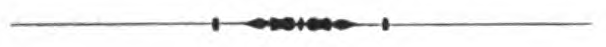
\includegraphics[width=49mm]{AB01-PDF0078-F01.png}\end{center}
\BeginSource{AB01-PDF0079}{}
\gdef\leftfolio{LXX}
\begin{minipage}[t]{\textwidth}
\vspace{13mm}
% AB01-PDF0079-body-L001
\SourceLine{AB01-PDF0079-body-L001}{\hbox to \linewidth{\hfil{\fontsize{18}{22}\selectfont ADDENDA ET EMENDANDA}\hfil}}
\vspace{9mm}
% AB01-PDF0079-body-L002
\SourceLine{AB01-PDF0079-body-L002}{Pag. VIII: Dimidia fere pars praefationis iam impressa erat, cum prodiit {\addfontfeatures{LetterSpace=1.0} Ibn al-Qifṭī’s} {\itshape Ta’-}}
% AB01-PDF0079-body-L003
\SourceLine{AB01-PDF0079-body-L003}{{\itshape rīḫ al-ḥukamā’ herausgegeben von J. Lippert}, Leipzig 1903; dolendum est quod saepe}
% AB01-PDF0079-body-L004
\SourceLine{AB01-PDF0079-body-L004}{editor varias lectiones et additamenta codicum indicare negligat. In Albatenii vita, p. 280–}
% AB01-PDF0079-body-L005
\SourceLine{AB01-PDF0079-body-L005}{–281, post verba « [cognomine] al-Battānī notus » haec adduntur, procul dubio in per-}
% AB01-PDF0079-body-L006
\SourceLine{AB01-PDF0079-body-L006}{paucis codicibus exstantia (cfr. {\addfontfeatures{LetterSpace=1.0} Chwolsohn}, I, 611, adn. 1): « et in libro iudicis Ṣā‘id}
% AB01-PDF0079-body-L007
\SourceLine{AB01-PDF0079-body-L007}{« al-Andalusī est {\itshape Abū Ǵa‘far} Muḥammad {\itshape ibn Sinān ibn Ǵābir} al-Ḥarrānī, [cognomine]}
% AB01-PDF0079-body-L008
\SourceLine{AB01-PDF0079-body-L008}{« al-Battānī notus ». Post illa « eorum motibus investigandis adaequaverit » editio Lippert}
% AB01-PDF0079-body-L009
\SourceLine{AB01-PDF0079-body-L009}{praebet etiam: « Studium praeterea in iudiciis astrorum collocaverat, quod eum impulit}
% AB01-PDF0079-body-L010
\SourceLine{AB01-PDF0079-body-L010}{« ad [libros] de hac re conscribendos; ex eius scriptis de [iudiciis] illis est liber ad ex-}
% AB01-PDF0079-body-L011
\SourceLine{AB01-PDF0079-body-L011}{« plicandam Tetrabiblum Ptolemaei ». Editio Lippert demum lectionem libri {\itshape al-Fihrist}}
% AB01-PDF0079-body-L012
\SourceLine{AB01-PDF0079-body-L012}{sequitur quam p. VIII, adn. 8 memoravi.}
% AB01-PDF0079-body-L013
\SourceLine{AB01-PDF0079-body-L013}{Nomen Abū Ǵa‘far pro Abū ‘Abd Allāh etiam in vita Abū Ma‘shar ({\addfontfeatures{LetterSpace=1.0} Ibn al-Qifṭī}}
% AB01-PDF0079-body-L014
\SourceLine{AB01-PDF0079-body-L014}{ed. Lippert p. 153) occurrit, probabiliter ex eiusdem Ṣā‘id al-Andalusī (de quo p. IX, adn. 4,}
% AB01-PDF0079-body-L015
\SourceLine{AB01-PDF0079-body-L015}{dixi) auctoritate. Ut videtur, false; nam Abū ‘Abd Allāh non solum reliqui biographi, sed}
% AB01-PDF0079-body-L016
\SourceLine{AB01-PDF0079-body-L016}{etiam {\addfontfeatures{LetterSpace=1.0} al-Mas‘ūdī}, {\itshape Prairies}, IX, 49, et {\addfontfeatures{LetterSpace=1.0} Ibn Yūnus}, introd. (apud {\addfontfeatures{LetterSpace=1.0} Caussin}, p. 72),}
% AB01-PDF0079-body-L017
\SourceLine{AB01-PDF0079-body-L017}{confirmant. Perperam etiam nomina Sinān et Ǵābir apud Ṣā‘id esse transposita, latissime}
% AB01-PDF0079-body-L018
\SourceLine{AB01-PDF0079-body-L018}{e concorde tot Arabicorum scriptorum traditione apparet.}
% AB01-PDF0079-body-L019
\SourceLine{AB01-PDF0079-body-L019}{VIII, adn. 7: In edit. Lippert p. 155–56. Dicitur Ibn al-Muktafī mortuus esse die Martis 4 ṣa-}
% AB01-PDF0079-body-L020
\SourceLine{AB01-PDF0079-body-L020}{far 377; sed 4 ṣafar illius anni fuit die Dominica 5 Iunii 987 Chr., iuxta civilem usum.}
% AB01-PDF0079-body-L021
\SourceLine{AB01-PDF0079-body-L021}{XV, adn. 3: in nonnullis exemplaribus {\itshape Subbī} et \sourceglyph{AB01-PDF0079-G01} pro {\itshape Ṣubbī} et \sourceglyph{AB01-PDF0079-G02} impressum est.}
% AB01-PDF0079-body-L022
\SourceLine{AB01-PDF0079-body-L022}{XXIV–XXV: Non solum al-Battānī, sed etiam al-Bīrūnī in magno suo {\itshape Canone} Almagestum in}
% AB01-PDF0079-body-L023
\SourceLine{AB01-PDF0079-body-L023}{compendium redegisse affirmat {\addfontfeatures{LetterSpace=1.0} Ibn al-Qifṭī} l. c. (ed. Lippert, p. 97).}
% AB01-PDF0079-body-L024
\SourceLine{AB01-PDF0079-body-L024}{XXVI, l. 5: edit. Lippert, p. 242.}
% AB01-PDF0079-body-L025
\SourceLine{AB01-PDF0079-body-L025}{XXXIII, adn. 1: edit. Lippert, p. 326.}
% AB01-PDF0079-body-L026
\SourceLine{AB01-PDF0079-body-L026}{Pag. 3, lin. 14, pro {\itshape longiquitate} l. {\itshape longinquitate}.}
% AB01-PDF0079-body-L027
\SourceLine{AB01-PDF0079-body-L027}{6,11, pro {\itshape his causis antiqui diviserunt: quia.....} l. {\itshape antiqui diviserunt, pluribus innitentes}}
% AB01-PDF0079-body-L028
\SourceLine{AB01-PDF0079-body-L028}{{\itshape causis: quia scilicet.....}}
% AB01-PDF0079-body-L029
\SourceLine{AB01-PDF0079-body-L029}{6,32–36, ita ad verbum reddendum: {\itshape Significatio multiplicationis est quod sibi ipsi adiicias}}
% AB01-PDF0079-body-L030
\SourceLine{AB01-PDF0079-body-L030}{{\itshape alterum numerorum iuxta quantitatem unitatum alterius; intelligo multiplicationem}}
% AB01-PDF0079-body-L031
\SourceLine{AB01-PDF0079-body-L031}{{\itshape unitatum in unitates. Multiplicatio fractionum in unitates est quod sibi ipsi adiicias}}
% AB01-PDF0079-body-L032
\SourceLine{AB01-PDF0079-body-L032}{{\itshape fractiones iuxta quantitatem unitatum, vel quod dividas unitates iuxta quantitatem}}
% AB01-PDF0079-body-L033
\SourceLine{AB01-PDF0079-body-L033}{{\itshape fractionum ex uno. Multiplicatio fractionum in fractiones est quod dividas alteram}}
% AB01-PDF0079-body-L034
\SourceLine{AB01-PDF0079-body-L034}{{\itshape fractionum, quamcumque volueris, iuxta quantitatem alterius fractionis ex uno.}}
% AB01-PDF0079-body-L035
\SourceLine{AB01-PDF0079-body-L035}{Quod {\itshape sibi ipsi adiicere} verti, Arabice est {\itshape ḍā‘afa}, tum {\itshape duplicare} significans, tum}
% AB01-PDF0079-body-L036
\SourceLine{AB01-PDF0079-body-L036}{quantitatem datam {\itshape pluries sumere} ut eius multiplum proveniat; cfr. lexicographorum}
% AB01-PDF0079-body-L037
\SourceLine{AB01-PDF0079-body-L037}{Arabicorum definitiones apud {\addfontfeatures{LetterSpace=1.0} Lane}, {\itshape Arabic–english Lexicon}, s. v. Plato recte: {\itshape coacer-}}
% AB01-PDF0079-body-L038
\SourceLine{AB01-PDF0079-body-L038}{{\itshape vatio et aggregatio}. Sed alii Latini interpretes aevi medii semper {\itshape duplicare} vertunt; ita}
\end{minipage}
\BeginSource{AB01-PDF0080}{ADDENDA ET EMENDANDA}
\gdef\rightfolio{LXXI}
\begin{minipage}[t]{\textwidth}
% AB01-PDF0080-body-L001
\SourceLine{AB01-PDF0080-body-L001}{{\addfontfeatures{LetterSpace=1.0} Algoritmi} [i. e. al-Khuwārizmī] {\itshape de numero Indorum}: « necesse est omni numero}
% AB01-PDF0080-body-L002
\SourceLine{AB01-PDF0080-body-L002}{« qui multiplicatur in aliquo quolibet numero, ut {\itshape duplicetur} unus ex eis secundum uni-}
% AB01-PDF0080-body-L003
\SourceLine{AB01-PDF0080-body-L003}{« tates alterius » ({\itshape Trattati d’aritmetica pubblicati da B. Boncompagni}, Roma 1857,}
% AB01-PDF0080-body-L004
\SourceLine{AB01-PDF0080-body-L004}{p. 10). Similiter ex voce Arabica male versa factum est ut mathematici {\addfontfeatures{LetterSpace=1.0} Iudaei} XII sae-}
% AB01-PDF0080-body-L005
\SourceLine{AB01-PDF0080-body-L005}{culi, sicut Abrāhām bar Ḥiyyā’ et Abrāhām Ibn ‘Ezrā, Hebraice « multiplicare » dicerent}
% AB01-PDF0080-body-L006
\SourceLine{AB01-PDF0080-body-L006}{{\itshape kāphal} (i. e. duplicare), et « multiplicationem » {\itshape kephel} (i. e. duplicatio); exempla apud}
% AB01-PDF0080-body-L007
\SourceLine{AB01-PDF0080-body-L007}{{\addfontfeatures{LetterSpace=1.0} Steinschneider}, {\itshape Abraham ibn Esra}, in periodico Abhandlungen zur Geschichte der}
% AB01-PDF0080-body-L008
\SourceLine{AB01-PDF0080-body-L008}{Mathematik, t. III, 1880, p. 106 (adn. 179) et 113. Item usus vocis {\itshape kephel} ad adverbia mul-}
% AB01-PDF0080-body-L009
\SourceLine{AB01-PDF0080-body-L009}{tiplicantia exprimenda (ut {\itshape volta} apud Italos, {\itshape mal} apud Germanos) non a verbo ipso {\itshape kāphal}}
% AB01-PDF0080-body-L010
\SourceLine{AB01-PDF0080-body-L010}{ducendus, ut Steinschneider (1) putat, sed ab Arabico {\itshape ḍi‘f} « duplum rei, aut quantitas alteri}
% AB01-PDF0080-body-L011
\SourceLine{AB01-PDF0080-body-L011}{datae aequalis », quod eodem sensu usurpatur; cfr. apud {\addfontfeatures{LetterSpace=1.0} al-Battānī} ipsum t. III, p. 88:}
% AB01-PDF0080-body-L012
\SourceLine{AB01-PDF0080-body-L012}{\textarabic{\upshape وتَضَاعَفَ البُعْدُ اضْعَافًا كثيرة} et \textarabic{\upshape اعظم منه بأضعاف مُضْعَفَة} (2).}
% AB01-PDF0080-body-L013
\SourceLine{AB01-PDF0080-body-L013}{6,ult., pro {\itshape 1165} l. {\itshape 1135}.}
% AB01-PDF0080-body-L014
\SourceLine{AB01-PDF0080-body-L014}{9,39, pro {\itshape supplementaris} l. {\itshape supplementaris alterius}.}
% AB01-PDF0080-body-L015
\SourceLine{AB01-PDF0080-body-L015}{11,3 a f., pro {\itshape complementi} l. {\itshape dupli complementi}.}
% AB01-PDF0080-body-L016
\SourceLine{AB01-PDF0080-body-L016}{13, adn. 2: « Ordines » Lunae a {\addfontfeatures{LetterSpace=1.0} Vettio Valente} (de quo p. 309, adn. 5) in primo {\itshape Astro-}}
% AB01-PDF0080-body-L017
\SourceLine{AB01-PDF0080-body-L017}{{\itshape logiae} libro, cap. \textgreek{περὶ εὑρέσεως βαθμῶν καὶ ἀνέμων τῆς σελήνης} exhiberi, testis est {\addfontfeatures{LetterSpace=1.0} Cl. Sal-}}
% AB01-PDF0080-body-L018
\SourceLine{AB01-PDF0080-body-L018}{{\addfontfeatures{LetterSpace=1.0} masius}, {\itshape De annis climactericis et antiqua astrologia diatribae}, Lugduni Batavorum}
% AB01-PDF0080-body-L019
\SourceLine{AB01-PDF0080-body-L019}{1648, p. 61, qui non satis perspicue dicit: « \textgreek{Βαθμοὶ} Lunae sunt qui per latitudinem Zo-}
% AB01-PDF0080-body-L020
\SourceLine{AB01-PDF0080-body-L020}{« diaci numerantur, dum ea a septentrione ad meridiem meat aut a meridie rursus ad}
% AB01-PDF0080-body-L021
\SourceLine{AB01-PDF0080-body-L021}{« septentrionem ascendendo et descendendo, modo ad Austrum, modo ad Aquilonem ».—}
% AB01-PDF0080-body-L022
\SourceLine{AB01-PDF0080-body-L022}{Etiam apud {\addfontfeatures{LetterSpace=1.0} Iulianum Laodicensem} (\textgreek{Ἰουλιανὸς Λαοδικεύς}), incertae inter IV et VI}
% AB01-PDF0080-body-L023
\SourceLine{AB01-PDF0080-body-L023}{saec. Chr. aetatis, \textgreek{βαθμοί} Solis, Lunae, quinque planetarum occurrunt; quanam ratione}
% AB01-PDF0080-body-L024
\SourceLine{AB01-PDF0080-body-L024}{computati bene non liquet. Vide excerpta in {\itshape Catal. codd. astrolog. Graecorum}, IV (1903),}
% AB01-PDF0080-body-L025
\SourceLine{AB01-PDF0080-body-L025}{p. 106–108.}
% AB01-PDF0080-body-L026
\SourceLine{AB01-PDF0080-body-L026}{29,36, pro \sourceglyph{AB01-PDF0080-G01} l. {\itshape terrestrium}.}
% AB01-PDF0080-body-L027
\SourceLine{AB01-PDF0080-body-L027}{41, adn. 2: Idem Albatenii error apud nonnullos etiam aetatis nostrae scriptores, e quibus}
% AB01-PDF0080-body-L028
\SourceLine{AB01-PDF0080-body-L028}{R. {\addfontfeatures{LetterSpace=1.0} Wolf}. {\itshape Handbuch der Astronomie}, t. I, p. 443, § 202,e.}
% AB01-PDF0080-body-L029
\SourceLine{AB01-PDF0080-body-L029}{54,26, pro {\itshape utemus} l. {\itshape utemur}.}
% AB01-PDF0080-body-L030
\SourceLine{AB01-PDF0080-body-L030}{54,28, pro {\itshape quantitas} l. {\itshape argumentum}.}
% AB01-PDF0080-body-L031
\SourceLine{AB01-PDF0080-body-L031}{54, adn. 10, pro {\itshape quantitate} l. {\itshape argumento}.}
% AB01-PDF0080-body-L032
\SourceLine{AB01-PDF0080-body-L032}{68,23, pro {\itshape qu} l. {\itshape qui}.}
% AB01-PDF0080-body-L033
\SourceLine{AB01-PDF0080-body-L033}{71,4–5, emendetur iuxta quae dixi p. 322, adn. 2.}
% AB01-PDF0080-body-L034
\SourceLine{AB01-PDF0080-body-L034}{75, de voce {\itshape ǵawzahar} in titulo cap. XXXVII, fortasse interpolata, vide p. XLIII praefationis.}
% AB01-PDF0080-body-L035
\SourceLine{AB01-PDF0080-body-L035}{80,38, pro {\itshape octavam} l. {\itshape decimam octavam}, ut Plato habet; cfr. p. 257–58, et XXXVIII, adn. 3.}
% AB01-PDF0080-body-L036
\SourceLine{AB01-PDF0080-body-L036}{80, adn. 4, pro {\itshape sequenttnus} l. {\itshape sequentibus}.}
% AB01-PDF0080-body-L037
\SourceLine{AB01-PDF0080-body-L037}{85,23–24, verba {\itshape in semidiametrum multiplica, et productum} delenda sunt; cfr. p. 265.}
% AB01-PDF0080-body-L038
\SourceLine{AB01-PDF0080-body-L038}{96,6, pro {\itshape horae}, quod cod. et Pl. habent, videtur {\itshape gradus} legendum; cfr. p. 275, adn. 1.}
% AB01-PDF0080-body-L039
\SourceLine{AB01-PDF0080-body-L039}{107,10, pro {\itshape consuemus} l. {\itshape consuescimus}.}
% AB01-PDF0080-body-L040
\SourceLine{AB01-PDF0080-body-L040}{114,11, in minutis apogei Martis pro {\itshape 18′} l. {\itshape 58′}.}
% AB01-PDF0080-body-L041
\SourceLine{AB01-PDF0080-body-L041}{114, adn. 1: Transpositio nonnisi in editionibus Platonis; cfr. praefationem p. LV.}
\NotesStart
\noindent\begin{minipage}[t]{.485\linewidth}\fontsize{10}{12.25}\selectfont
% AB01-PDF0080-notes_left-L001
\SourceLine{AB01-PDF0080-notes_left-L001}{(1) L. c., p. 106, et {\itshape Intorno ad alcuni mate-}}
% AB01-PDF0080-notes_left-L002
\SourceLine{AB01-PDF0080-notes_left-L002}{{\itshape matici del medio evo, lettere a B. Boncompagni},}
% AB01-PDF0080-notes_left-L003
\SourceLine{AB01-PDF0080-notes_left-L003}{Roma 1863–67, Lettera IV (Brani dell’aritmetica di}
% AB01-PDF0080-notes_left-L004
\SourceLine{AB01-PDF0080-notes_left-L004}{Elia Misrachi) p. 54, adn. 1, et p 65, adn. 1.}
\end{minipage}\hfill\begin{minipage}[t]{.485\linewidth}\fontsize{10}{12.25}\selectfont
% AB01-PDF0080-notes_right-L001
\SourceLine{AB01-PDF0080-notes_right-L001}{(2) Plerumque \textarabic{\upshape مرة} usurpat (t. III, p. 88-92, 182-}
% AB01-PDF0080-notes_right-L002
\SourceLine{AB01-PDF0080-notes_right-L002}{–185); t. III, p. 183 etiam \textarabic{\upshape مِثْل}. pl. \textarabic{\upshape امثال}. Locis pa-}
% AB01-PDF0080-notes_right-L003
\SourceLine{AB01-PDF0080-notes_right-L003}{rallelis, {\addfontfeatures{LetterSpace=1.0} Ibn Rosteh} p. 18–21, et {\addfontfeatures{LetterSpace=1.0} al-Farghānī}}
% AB01-PDF0080-notes_right-L004
\SourceLine{AB01-PDF0080-notes_right-L004}{ed. Golii p. 81–82, promiscue \textarabic{\upshape مثل} et \textarabic{\upshape مرة} habent.}
\end{minipage}
\end{minipage}
\BeginSource{AB01-PDF0081}{ADDENDA ET EMENDANDA}
\gdef\leftfolio{LXXII}
\begin{minipage}[t]{\textwidth}
% AB01-PDF0081-body-L001
\SourceLine{AB01-PDF0081-body-L001}{124,2, pro {\itshape referta} l. {\itshape relata}.}
% AB01-PDF0081-body-L002
\SourceLine{AB01-PDF0081-body-L002}{129, marg., numerus paginae textus, male impressus, est {\itshape 194}.}
% AB01-PDF0081-body-L003
\SourceLine{AB01-PDF0081-body-L003}{132,6, pro {\itshape interiectos} l. {\itshape interiectis}.}
% AB01-PDF0081-body-L004
\SourceLine{AB01-PDF0081-body-L004}{133,29, pro {\itshape cognoscuntur. Idest} l. {\itshape cognoscuntur; idest.}}
% AB01-PDF0081-body-L005
\SourceLine{AB01-PDF0081-body-L005}{133,31, pro {\itshape deprehende; si} l. {\itshape deprehendes. — Si.}}
% AB01-PDF0081-body-L006
\SourceLine{AB01-PDF0081-body-L006}{134,18, post {\itshape consistit} haec inserantur: [{\itshape distantiam multiplica in tempora horaria gradus}}
% AB01-PDF0081-body-L007
\SourceLine{AB01-PDF0081-body-L007}{{\itshape sequentis}]. Cfr. p. 316, adn. 3.}
% AB01-PDF0081-body-L008
\SourceLine{AB01-PDF0081-body-L008}{134,ult.: Verba {\itshape hoc modo hilegia} etc., fortasse spuria; cfr. praefationem p. XLIII.}
% AB01-PDF0081-body-L009
\SourceLine{AB01-PDF0081-body-L009}{138–139, adn. 5: Additamenta quorumdam codicum Platonis legantur in praefatione p. LII–LV.}
% AB01-PDF0081-body-L010
\SourceLine{AB01-PDF0081-body-L010}{139,10, emendandum sicut p. 321 docui.}
% AB01-PDF0081-body-L011
\SourceLine{AB01-PDF0081-body-L011}{148,1, addatur in margine {\itshape p. 223} textus Arabici.}
% AB01-PDF0081-body-L012
\SourceLine{AB01-PDF0081-body-L012}{149,21 et 26–27, emendandae sicut p. 326 exposui.}
% AB01-PDF0081-body-L013
\SourceLine{AB01-PDF0081-body-L013}{158,6 a f. (notis non supputatis) pro {\itshape quos} l. {\itshape quoque}.}
% AB01-PDF0081-body-L014
\SourceLine{AB01-PDF0081-body-L014}{158,5 a f. (notis non supputatis) pro {\itshape tempore} l. {\itshape partem}.}
% AB01-PDF0081-body-L015
\SourceLine{AB01-PDF0081-body-L015}{162–163: Mirae Theonis definitiones sunt etiam in inedita {\addfontfeatures{LetterSpace=1.0} Vettii Valentis} {\itshape Astrologia},}
% AB01-PDF0081-body-L016
\SourceLine{AB01-PDF0081-body-L016}{lib. II, cap. de ventis stellarum (\textgreek{περὶ ἀνέμων τῶν ἀστέρων}). Nam, {\addfontfeatures{LetterSpace=1.0} Salmasio} ({\itshape de annis}}
% AB01-PDF0081-body-L017
\SourceLine{AB01-PDF0081-body-L017}{{\itshape climactericis} p. 421–22) teste, Valens, cum ceteris astrologis ponens Solem in 19° Arietis}
% AB01-PDF0081-body-L018
\SourceLine{AB01-PDF0081-body-L018}{exaltari (\textgreek{ὑψοῦσθαι}), indeque tetragonum considerans cuius vertices 19° Arietis, 19° Cancri,}
% AB01-PDF0081-body-L019
\SourceLine{AB01-PDF0081-body-L019}{19° Librae, 19° Capricorni, dicit a 19° Arietis ad totidem Cancri Solem \textgreek{καταβαίνειν τὸν}}
% AB01-PDF0081-body-L020
\SourceLine{AB01-PDF0081-body-L020}{\textgreek{βοῤῥᾶν}, a 19° Cancri ad similem gradum Librae \textgreek{καταβαίνειν τὸν νότον}, a 19° Librae ad 19°}
% AB01-PDF0081-body-L021
\SourceLine{AB01-PDF0081-body-L021}{Capricorni \textgreek{ἀναβαίνειν τὸν νότον}, a 19° Capricorni ad totidem Arietis \textgreek{βοῤῥᾶν ἀναβαίνειν}. Et}
% AB01-PDF0081-body-L022
\SourceLine{AB01-PDF0081-body-L022}{similia de reliquis planetis. Lunam diversam ita considerat lib. I, cap. \textgreek{περὶ εὑρέσεως βαθμῶν καὶ ἀνέ-}}
% AB01-PDF0081-body-L023
\SourceLine{AB01-PDF0081-body-L023}{\textgreek{μων τῆς σελήνης} (teste {\addfontfeatures{LetterSpace=1.0} Salmasio} p. 422) a Leone ad Libram \textgreek{καταβαίνειν τὰ βόρεια}, a}
% AB01-PDF0081-body-L024
\SourceLine{AB01-PDF0081-body-L024}{Scorpio ad Cancrum \textgreek{καταβαίνειν τὰ νότια}, ab Aquario ad Arietem \textgreek{ἀναβαίνειν τὰ νότια}, a}
% AB01-PDF0081-body-L025
\SourceLine{AB01-PDF0081-body-L025}{Tauro ad Cancrum \textgreek{ἀναβαίνειν τὰ βόρεια}; quae propterea Valentem dixisse arbitror, quod}
% AB01-PDF0081-body-L026
\SourceLine{AB01-PDF0081-body-L026}{Luna, iuxta astrologos, in 3° Tauri exaltatur; tetragoni vertices sunt igitur Taurus, Leo,}
% AB01-PDF0081-body-L027
\SourceLine{AB01-PDF0081-body-L027}{Scorpius, Aquarius. — Cum usu Albateniano consentit {\addfontfeatures{LetterSpace=1.0} Iulianus Laodicensis}, loco}
% AB01-PDF0081-body-L028
\SourceLine{AB01-PDF0081-body-L028}{antea (p. LXXI) memorato affirmans Solem, Venerem, Mercurium in 214°8′50″, 231°28′,}
% AB01-PDF0081-body-L029
\SourceLine{AB01-PDF0081-body-L029}{224°32′ longitudinis exstantes « in austrum descendere » (\textgreek{κατέρχεται νότον}), Lunam et Sa-}
% AB01-PDF0081-body-L030
\SourceLine{AB01-PDF0081-body-L030}{turnum, in 48°10′ et 24°28′, « in boream ascendere » (\textgreek{ἀνέρχεται βοῤῥᾶν}). Librarii corrupte-}
% AB01-PDF0081-body-L031
\SourceLine{AB01-PDF0081-body-L031}{lam inesse puto in Iove (154°12′) et Marte (137°35′), qui quoque dicuntur \textgreek{ἀνέρχεται βοῤῥᾶν}.}
% AB01-PDF0081-body-L032
\SourceLine{AB01-PDF0081-body-L032}{163–164, adn. {\itshape b}: Item {\addfontfeatures{LetterSpace=1.0} al-Khāzinī} f. 151,r.–v., et {\addfontfeatures{LetterSpace=1.0} Kūshiyār ibn Labbān} (loco quem}
% AB01-PDF0081-body-L033
\SourceLine{AB01-PDF0081-body-L033}{p. 325 memoravi) tabulam ascensionum rectarum ab initio Capricorni supputatarum prae-}
% AB01-PDF0081-body-L034
\SourceLine{AB01-PDF0081-body-L034}{bent. Unum problematum libri {\itshape de saphaea}, cuius auctor {\addfontfeatures{LetterSpace=1.0} az-Zarqālī}, est: longitudinem}
% AB01-PDF0081-body-L035
\SourceLine{AB01-PDF0081-body-L035}{stellae cognoscere ex ascensione recta ab initio Capricorni supputata (i. e. ex gradu cum}
% AB01-PDF0081-body-L036
\SourceLine{AB01-PDF0081-body-L036}{quo stella culminat) et declinatione; quae male vertit {\addfontfeatures{LetterSpace=1.0} Steinschneider}, {\itshape Études sur}}
% AB01-PDF0081-body-L037
\SourceLine{AB01-PDF0081-body-L037}{{\itshape Zarkali}, Bullett. di bibliografia, t. XVIII, 1885–86, p. 345 (= p. 57 libri seorsum editi).}
% AB01-PDF0081-body-L038
\SourceLine{AB01-PDF0081-body-L038}{Ab initio Capricorni tabulas ascensionum rectarum pro singulis zodiaci minutis supputavit}
% AB01-PDF0081-body-L039
\SourceLine{AB01-PDF0081-body-L039}{quoque {\addfontfeatures{LetterSpace=1.0} Abū Bakr ibn al-Musharraf}, IX heg. saeculo (XV Chr.) ut videtur ({\itshape Ca-}}
% AB01-PDF0081-body-L040
\SourceLine{AB01-PDF0081-body-L040}{{\itshape tal. Bibliothecae Kahirensis}, t. V, p. 238, mīqāt nr. 209). Et ab eodem Capricorni puncto}
% AB01-PDF0081-body-L041
\SourceLine{AB01-PDF0081-body-L041}{ascensiones 112 stellarum fixarum, pro anno 1650 Chr. circiter, numeravit {\addfontfeatures{LetterSpace=1.0} Muḥammad}}
% AB01-PDF0081-body-L042
\SourceLine{AB01-PDF0081-body-L042}{{\addfontfeatures{LetterSpace=1.0} al-Akhṣāṣī} Aegyptius in libello {\itshape al-durrah al-muḍī’ah fī ’l-a‘māl ash-shamsiyyah},}
% AB01-PDF0081-body-L043
\SourceLine{AB01-PDF0081-body-L043}{cuius duo exemplaria etiam in {\itshape Catal. Kahirensi} V, 245, mīqāt nr. 60 et 81; vide tabulas}
% AB01-PDF0081-body-L044
\SourceLine{AB01-PDF0081-body-L044}{editas ab {\addfontfeatures{LetterSpace=1.0} Edw. Knobel}, {\itshape On a catalogue of stars in the Calendarium of Mohammad}}
% AB01-PDF0081-body-L045
\SourceLine{AB01-PDF0081-body-L045}{{\itshape Al Achsasi Al Mouakket}, in Monthly Notices of the R. Astronomical Society, vol. LV,}
% AB01-PDF0081-body-L046
\SourceLine{AB01-PDF0081-body-L046}{Nr. 8, 1895, p. 429.}
\end{minipage}
\BeginSource{AB01-PDF0082}{ADDENDA ET EMENDANDA}
\gdef\rightfolio{LXXIII}
\begin{minipage}[t]{\textwidth}
% AB01-PDF0082-body-L001
\SourceLine{AB01-PDF0082-body-L001}{169,3 a f. (adnotationibus non supputatis), pro {\itshape extensione} l. {\itshape extensionis}.}
% AB01-PDF0082-body-L002
\SourceLine{AB01-PDF0082-body-L002}{171, adn. 3: Vide praeterea J. {\addfontfeatures{LetterSpace=1.0} Canal}, {\itshape Tiaret, monographie ancienne et moderne} (Bulletin}
% AB01-PDF0082-body-L003
\SourceLine{AB01-PDF0082-body-L003}{trimestral de géographie et d’archéologie d’Oran, t. XX, 1900, p. 1–44).}
% AB01-PDF0082-body-L004
\SourceLine{AB01-PDF0082-body-L004}{175,13, numeri {\itshape 10} et {\itshape 9} inter se permutentur.}
% AB01-PDF0082-body-L005
\SourceLine{AB01-PDF0082-body-L005}{175, adn. 9, pro \sourceglyph{AB01-PDF0082-G01} l. \sourceglyph{AB01-PDF0082-G02}.}
% AB01-PDF0082-body-L006
\SourceLine{AB01-PDF0082-body-L006}{181,1–4: Theorema proportionalitatis sinuum angulorum ad latera opposita in triangulo recti-}
% AB01-PDF0082-body-L007
\SourceLine{AB01-PDF0082-body-L007}{lineo, tanquam res omnibus nota iam ab {\addfontfeatures{LetterSpace=1.0} al-Bīrūnī}, {\itshape Chron.} p. 184 text., 166 vers.,}
% AB01-PDF0082-body-L008
\SourceLine{AB01-PDF0082-body-L008}{commemoratur.}
% AB01-PDF0082-body-L009
\SourceLine{AB01-PDF0082-body-L009}{191,16, pro {\itshape ortographicam} l. {\itshape orthographicam}.}
% AB01-PDF0082-body-L010
\SourceLine{AB01-PDF0082-body-L010}{194,26, lineola excidit in fractione \(\frac{\cos L}{\cos\delta}\).}
% AB01-PDF0082-body-L011
\SourceLine{AB01-PDF0082-body-L011}{194, in paenultima formula pro « \(\sin\omega\) » l. « \(\sin\varepsilon\) ».}
% AB01-PDF0082-body-L012
\SourceLine{AB01-PDF0082-body-L012}{198,16–22 et adn. 1: Epistula illa non est Regiomontani ad Blanchinum, ut Delambre affirmat,}
% AB01-PDF0082-body-L013
\SourceLine{AB01-PDF0082-body-L013}{sed {\addfontfeatures{LetterSpace=1.0} Blanchini} ad Regiomontanum; nunc melius edita a {\addfontfeatures{LetterSpace=1.0} M. Curtze}, {\itshape Urkunden zur}}
% AB01-PDF0082-body-L014
\SourceLine{AB01-PDF0082-body-L014}{{\itshape Geschichte der Mathematik im Mittelalter und der Renaissance}, Leipzig 1902, t. I,}
% AB01-PDF0082-body-L015
\SourceLine{AB01-PDF0082-body-L015}{p. 240–41: « Vidi, per aliquos auctores doctrinam dari ad inveniendum declinationem}
% AB01-PDF0082-body-L016
\SourceLine{AB01-PDF0082-body-L016}{« stellarum habentium latitudinem, quorum doctrina est, accipere latitudinem stelle atque}
% AB01-PDF0082-body-L017
\SourceLine{AB01-PDF0082-body-L017}{« declinationem gradus ecliptice, in quo videtur stella esse, et si ambo sunt in eadem}
% AB01-PDF0082-body-L018
\SourceLine{AB01-PDF0082-body-L018}{« parte, septentrionali scilicet aut meridionali, ipsas copulare, si vero una fuerit meridio-}
% AB01-PDF0082-body-L019
\SourceLine{AB01-PDF0082-body-L019}{« nalis, altera vero septentrionalis, demere minorem a maiori, et quod post copulationem}
% AB01-PDF0082-body-L020
\SourceLine{AB01-PDF0082-body-L020}{« aut subtractionem perveniat, elongationem stelle ab equinoctiali nominant, cuius dicunt}
% AB01-PDF0082-body-L021
\SourceLine{AB01-PDF0082-body-L021}{« accipiendum esse sinum. Nam prima fronte doctrina ipsa videtur falsa, quare arcus lati-}
% AB01-PDF0082-body-L022
\SourceLine{AB01-PDF0082-body-L022}{« tudinis et arcus declinationis quilibet procedit a suo polo, et sunt duo diversi arcus se}
% AB01-PDF0082-body-L023
\SourceLine{AB01-PDF0082-body-L023}{« secantes supra centrum stelle, nec ex ipsis solam sinus [sic] aut cordam accipi potest.}
% AB01-PDF0082-body-L024
\SourceLine{AB01-PDF0082-body-L024}{« Dicunt etiam, dictum sinum multiplicari debere per sinum aut cordam residui maxime}
% AB01-PDF0082-body-L025
\SourceLine{AB01-PDF0082-body-L025}{« declinationis, et productum dividere per sinum residui sciti complementi declinationis}
% AB01-PDF0082-body-L026
\SourceLine{AB01-PDF0082-body-L026}{« ecliptice, et hoc modo dicunt, declinationem veram stelle cum sua latitudine invenire.}
% AB01-PDF0082-body-L027
\SourceLine{AB01-PDF0082-body-L027}{« Certe nescio hanc demonstrationem lineare, nec invenio {\addfontfeatures{LetterSpace=1.0} Albategni} ipsam demonstrasse,}
% AB01-PDF0082-body-L028
\SourceLine{AB01-PDF0082-body-L028}{« sed narrando regulam ipsam ultro concludit. Miror etiam de {\addfontfeatures{LetterSpace=1.0} Ioanne Anglicano} (1)}
% AB01-PDF0082-body-L029
\SourceLine{AB01-PDF0082-body-L029}{« peritissimo et docto, qui in suo comento supra tabulas Toletanas per {\addfontfeatures{LetterSpace=1.0} Arzachelem}}
% AB01-PDF0082-body-L030
\SourceLine{AB01-PDF0082-body-L030}{« constructas hoc affirmat absque demonstratione ».}
% AB01-PDF0082-body-L031
\SourceLine{AB01-PDF0082-body-L031}{199,12, adde: {\itshape ut cap. XXXIX, p. 78–79.}}
% AB01-PDF0082-body-L032
\SourceLine{AB01-PDF0082-body-L032}{202, ter in formulis \(\frac{\cos\beta}{2R}\) occurrit, quod emendandum \(\frac{\cos\beta}{R}\).}
% AB01-PDF0082-body-L033
\SourceLine{AB01-PDF0082-body-L033}{204, adn. {\itshape a}: Fractionem diei \(\frac{1}{130}\) Platonem scripsisse, non \(\frac{1}{131}\) ut editiones habent, elucet e}
% AB01-PDF0082-body-L034
\SourceLine{AB01-PDF0082-body-L034}{consensu codicis Vaticani, Parisiensis, Veneti (alios de hac re non consului), et libri qui}
% AB01-PDF0082-body-L035
\SourceLine{AB01-PDF0082-body-L035}{{\itshape Almagesti parvum} inscribitur (de quo praefat. p. XXVI–XXVII). Hic, f. 10,r., affirmat: « Egi-}
% AB01-PDF0082-body-L036
\SourceLine{AB01-PDF0082-body-L036}{« ptiorum antiquissimi ex babilonia sicut per suas considerationes deprehenderunt ipsum}
% AB01-PDF0082-body-L037
\SourceLine{AB01-PDF0082-body-L037}{« [anni tempus] ex .CCCLXV. diebus et quarta diei et una parte ex .CXXX. diei par-}
% AB01-PDF0082-body-L038
\SourceLine{AB01-PDF0082-body-L038}{« tibus constare dixerunt ». In exemplari suo Arabico Plato \textarabic{\upshape قل} 130 loco \textarabic{\upshape قك} 120 inve-}
% AB01-PDF0082-body-L039
\SourceLine{AB01-PDF0082-body-L039}{nisse videtur.}
% AB01-PDF0082-body-L040
\SourceLine{AB01-PDF0082-body-L040}{205, adn. 1, pro {\itshape al-Mumti‘} et {\itshape al-muqni‘} l. {\itshape al-Mumta‘} et {\itshape al-maqna‘}.}
\NotesStart
% AB01-PDF0082-notes_full-L001
\SourceLine{AB01-PDF0082-notes_full-L001}{(1) Eum {\addfontfeatures{LetterSpace=1.0} Curtze} monet esse {\addfontfeatures{LetterSpace=1.0} Iohannem Ashenton}, anno 1348 vivum. Nomen desideratur}
% AB01-PDF0082-notes_full-L002
\SourceLine{AB01-PDF0082-notes_full-L002}{in dissertationibus Steinschneiderianis de az-Zarqālī.}
\end{minipage}
\par\vspace{6pt}\hfill{\fontsize{8}{10}\selectfont 10*}
\BeginSource{AB01-PDF0083}{ADDENDA ET EMENDANDA}
\gdef\leftfolio{LXXIV}
\begin{minipage}[t]{\textwidth}
% AB01-PDF0083-body-L001
\SourceLine{AB01-PDF0083-body-L001}{215: E {\addfontfeatures{LetterSpace=1.0} Snellii} auctoritate, narrat {\addfontfeatures{LetterSpace=1.0} Montucla} ({\itshape Hist. des mathématiques}, nouvelle édition,}
% AB01-PDF0083-body-L002
\SourceLine{AB01-PDF0083-body-L002}{Paris, an VII–X, t. I, p. 366) az-Zarqālī, circa annos 1070–80 florentem, ad vitandam}
% AB01-PDF0083-body-L003
\SourceLine{AB01-PDF0083-body-L003}{incertam solstitiorum observationem, in calculo longitudinis apogei solaris usum esse ob-}
% AB01-PDF0083-body-L004
\SourceLine{AB01-PDF0083-body-L004}{servationibus Solis in ambobus aequinoctiis ac tertio quolibet eclipticae puncto, vel etiam}
% AB01-PDF0083-body-L005
\SourceLine{AB01-PDF0083-body-L005}{in tribus punctis quibuscumque. Est ratio igitur de qua al-Bīrūnī l. c. agit. Ex quo az-}
% AB01-PDF0083-body-L006
\SourceLine{AB01-PDF0083-body-L006}{-Zarqālī operum (quorum solus liber de saphaea, in versione Hispanica, typis excusus est)}
% AB01-PDF0083-body-L007
\SourceLine{AB01-PDF0083-body-L007}{Snellius talia compererit nescio.}
% AB01-PDF0083-body-L008
\SourceLine{AB01-PDF0083-body-L008}{216: Priore II saec. Chr. medietate, {\addfontfeatures{LetterSpace=1.0} Theon Smyrnaeus} (minime cum Alexandrino confun-}
% AB01-PDF0083-body-L009
\SourceLine{AB01-PDF0083-body-L009}{dendus) annum sideralem, quem a tropico non distinguit, ponit \(365\frac{1}{4}\) esse dierum; an-}
% AB01-PDF0083-body-L010
\SourceLine{AB01-PDF0083-body-L010}{num anomalisticum, quo Sol ad apogeum redit, \(365\frac{1}{2}\). Motum igitur praecessionis ne-}
% AB01-PDF0083-body-L011
\SourceLine{AB01-PDF0083-body-L011}{gans, manifeste putat apogeum solare totum zodiacum percurrere 1461 annis, i. e. \(27^{\prime}\,6^{\prime\prime}\,\frac{1}{2}\)}
% AB01-PDF0083-body-L012
\SourceLine{AB01-PDF0083-body-L012}{quotannis moveri! Unde haec absurda sumpserit nescimus; error in textu Graeco non potest}
% AB01-PDF0083-body-L013
\SourceLine{AB01-PDF0083-body-L013}{coniici, nam, ut {\addfontfeatures{LetterSpace=1.0} Martin} p. 110 animadvertit, auctor ipse addit Solem ad idem altitudinis}
% AB01-PDF0083-body-L014
\SourceLine{AB01-PDF0083-body-L014}{punctum, id est ad eandem a Terra distantiam, eadem diei hora singulis {\itshape bienniis} redire (1).}
% AB01-PDF0083-body-L015
\SourceLine{AB01-PDF0083-body-L015}{Recte igitur Martin l. c. iudicat: « Ecce vero Theon Smyrnaeus solaris apogei in}
% AB01-PDF0083-body-L016
\SourceLine{AB01-PDF0083-body-L016}{« zodiaco motum erga aequinoctia et erga stellas iam affirmaverat, et ita quidem iusto}
% AB01-PDF0083-body-L017
\SourceLine{AB01-PDF0083-body-L017}{« citiorem fecerat, ut satius fuerit eum ignorare aut negare, quam talem credere ».}
% AB01-PDF0083-body-L018
\SourceLine{AB01-PDF0083-body-L018}{218, adn. 1, pro {\itshape Riccii} l. {\itshape Ricii}.}
% AB01-PDF0083-body-L019
\SourceLine{AB01-PDF0083-body-L019}{226, adn. 2, pro {\itshape 1835} l. {\itshape 1836}.}
% AB01-PDF0083-body-L020
\SourceLine{AB01-PDF0083-body-L020}{237, adn. 1, pro {\itshape al-mumaththil} l. {\itshape al-mu‘addil}.}
% AB01-PDF0083-body-L021
\SourceLine{AB01-PDF0083-body-L021}{242, adn. 2: Nominis {\itshape Dhū ’l-qarnayn} originem explicaveram ad fidem complurium peritis-}
% AB01-PDF0083-body-L022
\SourceLine{AB01-PDF0083-body-L022}{simorum virorum, praesertim cum {\addfontfeatures{LetterSpace=1.0} Clemens Alexandrinus} valde queratur quod}
% AB01-PDF0083-body-L023
\SourceLine{AB01-PDF0083-body-L023}{Alexander se ad imaginem Dei, cornibus praeditum, effingi iusserit. Veram nominis ori-}
% AB01-PDF0083-body-L024
\SourceLine{AB01-PDF0083-body-L024}{ginem nunc illustrat {\addfontfeatures{LetterSpace=1.0} Fr. Kampers}, {\itshape Alexander der Grosse und die Idee des Weltim-}}
% AB01-PDF0083-body-L025
\SourceLine{AB01-PDF0083-body-L025}{{\itshape periums in Prophetie und Sage}, Freiburg i. Br. 1901, p. 71–85 (= Studien und Dar-}
% AB01-PDF0083-body-L026
\SourceLine{AB01-PDF0083-body-L026}{stellungen aus dem Gebiete der Geschichte hrsg. von H. Grauert, fasc. II–III). In fabulosis}
% AB01-PDF0083-body-L027
\SourceLine{AB01-PDF0083-body-L027}{Alexandri narrationibus quae apud Orientales, praesertim Syros, circumferebantur primis}
% AB01-PDF0083-body-L028
\SourceLine{AB01-PDF0083-body-L028}{saeculis aerae Christianae, Alexander tanquam novae aetatis instaurator mundique ser-}
% AB01-PDF0083-body-L029
\SourceLine{AB01-PDF0083-body-L029}{vator exhibetur, similis Messiae Hebraeorum; ei igitur duo cornua tributa sunt quae in}
% AB01-PDF0083-body-L030
\SourceLine{AB01-PDF0083-body-L030}{scriptis Iudaicis insigne Messiae dicuntur. Omnia ex antiquissimis Babylonicis opinionibus}
% AB01-PDF0083-body-L031
\SourceLine{AB01-PDF0083-body-L031}{profluunt, quae breviter exposita leguntur in libro {\addfontfeatures{LetterSpace=1.0} E. Schrader}, {\itshape Die Keilinschriften}}
% AB01-PDF0083-body-L032
\SourceLine{AB01-PDF0083-body-L032}{{\itshape und das Alte Testament, 3. Auflage neu bearbeitet von} {\addfontfeatures{LetterSpace=1.0} H. Zimmern} {\itshape und} {\addfontfeatures{LetterSpace=1.0} H. Winck-}}
% AB01-PDF0083-body-L033
\SourceLine{AB01-PDF0083-body-L033}{{\addfontfeatures{LetterSpace=1.0} ler}, Berlin 1902, p. 380–82; eadem causa, 25 saecula ante Alexandrum, Naram-Sin,}
% AB01-PDF0083-body-L034
\SourceLine{AB01-PDF0083-body-L034}{Babyloniae rex, duobus cornibus praeditus effictus erat.}
% AB01-PDF0083-body-L035
\SourceLine{AB01-PDF0083-body-L035}{243: De origine nominum complurium mensium Copticorum optime disseruit {\addfontfeatures{LetterSpace=1.0} A. Wiede-}}
% AB01-PDF0083-body-L036
\SourceLine{AB01-PDF0083-body-L036}{{\addfontfeatures{LetterSpace=1.0} mann}, {\itshape Zu den ägyptischen Monatsnamen} in Orientalistische Litteratur-Zeitung, t. VI,}
% AB01-PDF0083-body-L037
\SourceLine{AB01-PDF0083-body-L037}{1903, col. 5–7.}
% AB01-PDF0083-body-L038
\SourceLine{AB01-PDF0083-body-L038}{246, adn. {\itshape a}: Cfr. etiam Samps Pucharem, in animadvers. ad tabulas t. II, p. 72–77 adductum.}
% AB01-PDF0083-body-L039
\SourceLine{AB01-PDF0083-body-L039}{250, ad cap. XXXVII: Cfr. praefationem p. XLIII.}
% AB01-PDF0083-body-L040
\SourceLine{AB01-PDF0083-body-L040}{251,9: Falsum regulam non reperiri apud {\addfontfeatures{LetterSpace=1.0} Ptolemaeum}; hic enim V, 7 (ed. Halma I, 315)}
% AB01-PDF0083-body-L041
\SourceLine{AB01-PDF0083-body-L041}{ad supputandam tabulam latitudinis Lunae, « in hoc », ait, « eadem demonstratione (\textgreek{δείξει})}
% AB01-PDF0083-body-L042
\SourceLine{AB01-PDF0083-body-L042}{« usi sumus, qua iam supputavimus arcus circuli per polos aequatoris transeuntis, inter-}
% AB01-PDF0083-body-L043
\SourceLine{AB01-PDF0083-body-L043}{« ceptos aequatore et ecliptica », scilicet declinationes Solis.}
\NotesStart
\noindent\begin{minipage}[t]{.485\linewidth}\fontsize{10}{12.25}\selectfont
% AB01-PDF0083-notes_left-L001
\SourceLine{AB01-PDF0083-notes_left-L001}{(1) {\addfontfeatures{LetterSpace=1.0} Theonis Smyrnaei} {\itshape Liber de astro-}}
% AB01-PDF0083-notes_left-L002
\SourceLine{AB01-PDF0083-notes_left-L002}{{\itshape nomia, textum edidit, Latine vertit,..... notis illu-}}
% AB01-PDF0083-notes_left-L003
\SourceLine{AB01-PDF0083-notes_left-L003}{{\itshape stravit Th. H. Martin}, Parisiis 1849, p. 261; {\addfontfeatures{LetterSpace=1.0} Theo-}}
\end{minipage}\hfill\begin{minipage}[t]{.485\linewidth}\fontsize{10}{12.25}\selectfont
% AB01-PDF0083-notes_right-L001
\SourceLine{AB01-PDF0083-notes_right-L001}{{\addfontfeatures{LetterSpace=1.0} nis Smyrnaei} {\itshape Expositio rerum mathematica-}}
% AB01-PDF0083-notes_right-L002
\SourceLine{AB01-PDF0083-notes_right-L002}{{\itshape rum ad legendum Platonem utilium, recensuit}}
% AB01-PDF0083-notes_right-L003
\SourceLine{AB01-PDF0083-notes_right-L003}{{\itshape Ed. Hiller}, Lipsiae 1878, p. 172–73.}
\end{minipage}
\end{minipage}
\BeginSource{AB01-PDF0084}{ADDENDA ET EMENDANDA}
\gdef\rightfolio{LXXV}
\begin{minipage}[t]{\textwidth}
% AB01-PDF0084-body-L001
\SourceLine{AB01-PDF0084-body-L001}{262, adn. {\itshape s}: Discrepantias e diversa eclipticae obliquitate exorientes {\addfontfeatures{LetterSpace=1.0} al-Battānī} abstulit, in}
% AB01-PDF0084-body-L002
\SourceLine{AB01-PDF0084-body-L002}{tabulis (t. II, p. 95–101) singulis {\addfontfeatures{LetterSpace=1.0} Theonis} climatibus aliam latitudinem, novae obliqui-}
% AB01-PDF0084-body-L003
\SourceLine{AB01-PDF0084-body-L003}{tati quadrantem, assignans.}
% AB01-PDF0084-body-L004
\SourceLine{AB01-PDF0084-body-L004}{265, adn. 2: De nunciis Lunae Novae apud Hebraeos, qui testimonium mulierum, servorum}
% AB01-PDF0084-body-L005
\SourceLine{AB01-PDF0084-body-L005}{et improborum non recipiebant, cfr. {\addfontfeatures{LetterSpace=1.0} Maimonidis} librum {\itshape de novilunio}, cap. II, col. 240–}
% AB01-PDF0084-body-L006
\SourceLine{AB01-PDF0084-body-L006}{–244 editionis laudatae in praefatione p. XXXIV, adn. 3.}
% AB01-PDF0084-body-L007
\SourceLine{AB01-PDF0084-body-L007}{266, adn. 1: Pulcherrimum incertae rei exemplum apud {\addfontfeatures{LetterSpace=1.0} Aḥmad} ibn Khālid {\addfontfeatures{LetterSpace=1.0} an-Nāṣirī as-}}
% AB01-PDF0084-body-L008
\SourceLine{AB01-PDF0084-body-L008}{{\addfontfeatures{LetterSpace=1.0} -Salāwī}, {\itshape Al-istiqṣā’ li akhbār duwal al-Maghrib al-aqṣà}, Kahirae 1312 heg., t. IV,}
% AB01-PDF0084-body-L009
\SourceLine{AB01-PDF0084-body-L009}{p. 245. Nocte inter 28 et 29 diem mensis ramaḍān 1292 (28–29 Oct. 1875), duodecim}
% AB01-PDF0084-body-L010
\SourceLine{AB01-PDF0084-body-L010}{homines in urbe Rabāṭ imperii Maroccani dicunt se Lunam novam post occasum Solis}
% AB01-PDF0084-body-L011
\SourceLine{AB01-PDF0084-body-L011}{certissime vidisse. Testimonium eorum recipit qāḍī urbis, statimque scribit ad sultanum}
% AB01-PDF0084-body-L012
\SourceLine{AB01-PDF0084-body-L012}{Maroccanum prope urbem tunc commorantem. Ineunte 29 die omnes ieiunium desinunt.}
% AB01-PDF0084-body-L013
\SourceLine{AB01-PDF0084-body-L013}{Astronomi ({\itshape falakiyyūn}) aulici tamen asseverant illum diem nullo modo posse festum esse;}
% AB01-PDF0084-body-L014
\SourceLine{AB01-PDF0084-body-L014}{dubitatio igitur inter homines exoritur. Re vera, post occasum 29 diei, frustra omnes}
% AB01-PDF0084-body-L015
\SourceLine{AB01-PDF0084-body-L015}{Lunam novam in Caelo quaerunt, licet purissimus sit aer; denuo igitur ieiunium agunt}
% AB01-PDF0084-body-L016
\SourceLine{AB01-PDF0084-body-L016}{usque ad noctem 30 diei (iuxta nostrum supputandi usum), qua Luna nova tandem cer-}
% AB01-PDF0084-body-L017
\SourceLine{AB01-PDF0084-body-L017}{nitur. Illorum testium fraus inde elucet, qui in carcerem coniiciuntur.}
% AB01-PDF0084-body-L018
\SourceLine{AB01-PDF0084-body-L018}{272: Eodem libro V, 1, paulo ante locum adductum, {\addfontfeatures{LetterSpace=1.0} Aristoteles} haec narrat: « Qui manu}
% AB01-PDF0084-body-L019
\SourceLine{AB01-PDF0084-body-L019}{« sibi obumbrat, aut per fistulam aspicit, differentias colorum nec magis nec minus dis-}
% AB01-PDF0084-body-L020
\SourceLine{AB01-PDF0084-body-L020}{« tinguit, sed longinquius cernit. Item qui interdum e foveis ac puteis astra conspiciunt ».}
% AB01-PDF0084-body-L021
\SourceLine{AB01-PDF0084-body-L021}{Sinarum instrumentum fortasse est cum sphaera armillari globoque caelesti {\addfontfeatures{LetterSpace=1.0} Ger-}}
% AB01-PDF0084-body-L022
\SourceLine{AB01-PDF0084-body-L022}{{\addfontfeatures{LetterSpace=1.0} berti} comparandum, cuius polos transfigebat fistula ad constellationem Ursae Minoris}
% AB01-PDF0084-body-L023
\SourceLine{AB01-PDF0084-body-L023}{directa; eam describit {\addfontfeatures{LetterSpace=1.0} Günther}, l. c., p. 16–17.}
% AB01-PDF0084-body-L024
\SourceLine{AB01-PDF0084-body-L024}{Nescio an {\itshape tubos} significare voluerit voce {\itshape mir’āh} {\addfontfeatures{LetterSpace=1.0} Abū ’l-‘Alā’ al-Ma‘arrī}, poeta}
% AB01-PDF0084-body-L025
\SourceLine{AB01-PDF0084-body-L025}{celeberrimus anno 449 (inc. 9 Mart. 1057) mortuus, duobus locis quos {\addfontfeatures{LetterSpace=1.0} von Kremer},}
% AB01-PDF0084-body-L026
\SourceLine{AB01-PDF0084-body-L026}{{\itshape Culturgeschichte des Orients unter den Chalifen}, Wien 1875–77, t. II, p. 448 adducit.}
% AB01-PDF0084-body-L027
\SourceLine{AB01-PDF0084-body-L027}{Alter est (= {\itshape Luzūm mā lā yalzam}, Bombay 1303 heg., p. 155):}
% AB01-PDF0084-body-L028
\SourceLine{AB01-PDF0084-body-L028}{\hbox to \linewidth{\hfil
\includegraphics[width=.54\linewidth]{AB01-PDF0084-G01.png}\hfil}}
% AB01-PDF0084-body-L029
\SourceLine{AB01-PDF0084-body-L029}{\hbox to \linewidth{\hfil
\includegraphics[width=.54\linewidth]{AB01-PDF0084-G02.png}\hfil}}
% AB01-PDF0084-body-L030
\SourceLine{AB01-PDF0084-body-L030}{« mir’āh sume, ac sidera bene cognosce quae amarum faciunt saporem mellis ex al-}
% AB01-PDF0084-body-L031
\SourceLine{AB01-PDF0084-body-L031}{« veari collecti, [nam] procul dubio mortem portendunt, non vero resurrectionem ».}
% AB01-PDF0084-body-L032
\SourceLine{AB01-PDF0084-body-L032}{Altero loco ait {\itshape mir’āh} astronomi, licet parvum sit, ei tamen universum ostendere. Voca-}
% AB01-PDF0084-body-L033
\SourceLine{AB01-PDF0084-body-L033}{bulum plerumque {\itshape speculum} significat; qua re Kremer instrumentis astronomicis Arabum}
% AB01-PDF0084-body-L034
\SourceLine{AB01-PDF0084-body-L034}{« Spiegel von polirtem Metall » adnumerat. Vix recte. His locis genuinus vocabuli sensus}
% AB01-PDF0084-body-L035
\SourceLine{AB01-PDF0084-body-L035}{mihi restituendus videtur, scilicet {\itshape instrumenti quo res cernuntur}.}
% AB01-PDF0084-body-L036
\SourceLine{AB01-PDF0084-body-L036}{281, adn. {\itshape b}: Locus non ad {\itshape Tabulas Alphonsinas} pertinet, sed ad canones in easdem a {\addfontfeatures{LetterSpace=1.0} San-}}
% AB01-PDF0084-body-L037
\SourceLine{AB01-PDF0084-body-L037}{{\addfontfeatures{LetterSpace=1.0} tritter} conscriptos; cfr. meam praefationem p. XXXVI, adn. 7.}
% AB01-PDF0084-body-L038
\SourceLine{AB01-PDF0084-body-L038}{286–287: Eosdem Ibn Rosteh numeros invenio apud {\addfontfeatures{LetterSpace=1.0} Thābit ibn Qorrah}, eius coaevum,}
% AB01-PDF0084-body-L039
\SourceLine{AB01-PDF0084-body-L039}{in libello {\itshape in expositione Almagesti}, qui Latine tantum ac ineditus exstat (1). Nam mi-}
% AB01-PDF0084-body-L040
\SourceLine{AB01-PDF0084-body-L040}{nimae distantiae sunt: Lunae 33 radiorum terrestrium, Mercurii 64, Veneris 167, Solis}
% AB01-PDF0084-body-L041
\SourceLine{AB01-PDF0084-body-L041}{1079, Martis 1260, Iovis 8820, Saturni 14187; sed maxima Saturni minimaque fixarum}
\NotesStart
\noindent\begin{minipage}[t]{.485\linewidth}\fontsize{10}{12.25}\selectfont
% AB01-PDF0084-notes_left-L001
\SourceLine{AB01-PDF0084-notes_left-L001}{(1) Duobus codicibus Venetis utor, quos in prae-}
% AB01-PDF0084-notes_left-L002
\SourceLine{AB01-PDF0084-notes_left-L002}{fatione p. LXVIII litteris A et B designavi. In A libel-}
% AB01-PDF0084-notes_left-L003
\SourceLine{AB01-PDF0084-notes_left-L003}{lus f. 14,v.–21,v. codicis complectitur, distantiae et}
% AB01-PDF0084-notes_left-L004
\SourceLine{AB01-PDF0084-notes_left-L004}{moles f. 20,r.–v.; in B libellus, cui titulus {\itshape Thebith}}
\end{minipage}\hfill\begin{minipage}[t]{.485\linewidth}\fontsize{10}{12.25}\selectfont
% AB01-PDF0084-notes_right-L001
\SourceLine{AB01-PDF0084-notes_right-L001}{{\itshape ben chorath de hijs quae indigent expositione ante}}
% AB01-PDF0084-notes_right-L002
\SourceLine{AB01-PDF0084-notes_right-L002}{{\itshape quam legatur Almagester}, f. 49,v.,b–53,r.,b contine-}
% AB01-PDF0084-notes_right-L003
\SourceLine{AB01-PDF0084-notes_right-L003}{tur, distantiae et moles f. 52,r.–v.}
\end{minipage}
\end{minipage}
\BeginSource{AB01-PDF0085}{ADDENDA ET EMENDANDA}
\gdef\leftfolio{LXXVI}
\begin{minipage}[t]{\textwidth}
% AB01-PDF0085-body-L001
\SourceLine{AB01-PDF0085-body-L001}{17865 (pro 19880 et 20000 Ibn Rosteh). Moles autem: Solis 166, fixarum primae ma-}
% AB01-PDF0085-body-L002
\SourceLine{AB01-PDF0085-body-L002}{gnitudinis 94, Saturni et Iovis « quasi » 79, Martis « quasi » \(1\,{}^1\!/_2\), Veneris « quasi » \({}^1\!/_{87}\),}
% AB01-PDF0085-body-L003
\SourceLine{AB01-PDF0085-body-L003}{Lunae \({}^1\!/_{40}\) (A \({}^1\!/_{10}\)), Mercurii \({}^1\!/_{29680}\) (A \({}^1\!/_{29683}\)). Unde haec omnia sumpserit non dicit.}
% AB01-PDF0085-body-L004
\SourceLine{AB01-PDF0085-body-L004}{Eodem codice B, f. 54,v.,b–56,v.,a, alius etiam libellus inest: « {\itshape Incipit liber Thebith}}
% AB01-PDF0085-body-L005
\SourceLine{AB01-PDF0085-body-L005}{{\itshape « de quantitatibus stellarum et planetarum et proportio terre.} Ptholomeus et alij sa-}
% AB01-PDF0085-body-L006
\SourceLine{AB01-PDF0085-body-L006}{« pientes posuerunt corpus terre communem mensuram qua metiebantur stellarum cor-}
% AB01-PDF0085-body-L007
\SourceLine{AB01-PDF0085-body-L007}{« pora, et posuerunt medietatem diametri terre communem mensuram qua stellarum a}
% AB01-PDF0085-body-L008
\SourceLine{AB01-PDF0085-body-L008}{« centro terre longitudines mensurabant..... ». Breviter distantias Solis et Lunae a Pto-}
% AB01-PDF0085-body-L009
\SourceLine{AB01-PDF0085-body-L009}{lemaeo in eclipsibus repertas exponit; quo facto addit (f. 55,r.,a et b): « Dicit ergo {\addfontfeatures{LetterSpace=1.0} Ge-}}
% AB01-PDF0085-body-L010
\SourceLine{AB01-PDF0085-body-L010}{{\addfontfeatures{LetterSpace=1.0} « ber} ostensum est per hoc proportio [sic] cuiuscumque 2. diametrorum luminarium ad}
% AB01-PDF0085-body-L011
\SourceLine{AB01-PDF0085-body-L011}{« diametrum terre ». Sequuntur diametri corporum caelestium, eorum moles (« corpora »),}
% AB01-PDF0085-body-L012
\SourceLine{AB01-PDF0085-body-L012}{nec non eorum distantiae a centro Terrae in radiis terrestribus et in milliaribus (gradu}
% AB01-PDF0085-body-L013
\SourceLine{AB01-PDF0085-body-L013}{aequatoris \(56\,{}^3\!/_8\) milliariorum sumpto). Calculi ratio a ratione quam Albatenius refert}
% AB01-PDF0085-body-L014
\SourceLine{AB01-PDF0085-body-L014}{non discrepant, sed numeri cum al-Farghānī congruunt. — Demum latitudines septem}
% AB01-PDF0085-body-L015
\SourceLine{AB01-PDF0085-body-L015}{climatum Terrae exponit ad al-Farghānī fidem (« Alfragano » f. 56,r.,a); ultima verba}
% AB01-PDF0085-body-L016
\SourceLine{AB01-PDF0085-body-L016}{sunt: « Latitudo 7.\textsuperscript{i} climatis est trium graduum et 4.\textsuperscript{e} unius in celo, qui valent in terra}
% AB01-PDF0085-body-L017
\SourceLine{AB01-PDF0085-body-L017}{« 184. sed iste non est in terra, sed proximus ei maior scilicet ille 185. quia quoddam}
% AB01-PDF0085-body-L018
\SourceLine{AB01-PDF0085-body-L018}{« modicum remansit. Explicit tebith de quantitatibus stellarum ». Ob Alfragani et potis-}
% AB01-PDF0085-body-L019
\SourceLine{AB01-PDF0085-body-L019}{simum Gebri (Ǵābir ibn Aflaḥ) nomina, ac ob discrepantias a numeris alterius opusculi,}
% AB01-PDF0085-body-L020
\SourceLine{AB01-PDF0085-body-L020}{vehementissima suspicio subit libellum spurium esse. Alios codices indicat {\addfontfeatures{LetterSpace=1.0} Steinschnei-}}
% AB01-PDF0085-body-L021
\SourceLine{AB01-PDF0085-body-L021}{{\addfontfeatures{LetterSpace=1.0} der}, {\itshape Thabit ben Korra}, in Zeitschrift für Mathematik und Physik, XVIII, 1873, p. 337.}
% AB01-PDF0085-body-L022
\SourceLine{AB01-PDF0085-body-L022}{291,7 a f. (notis non supputatis): Alia exempla vocum {\itshape al-kātib} et {\itshape al-mukātib} pro Mercurio,}
% AB01-PDF0085-body-L023
\SourceLine{AB01-PDF0085-body-L023}{{\itshape al-muqātil} pro Saturno, passim occurrunt apud Maroccanum {\addfontfeatures{LetterSpace=1.0} Muḥammad as-Sūsī}}
% AB01-PDF0085-body-L024
\SourceLine{AB01-PDF0085-body-L024}{{\addfontfeatures{LetterSpace=1.0} al-Marghitī}, {\itshape al-Mumta‘ fī sharḥ al-maqna‘} et {\itshape al-Maṭla‘ ‘alà masā’il al-maqna‘}}
% AB01-PDF0085-body-L025
\SourceLine{AB01-PDF0085-body-L025}{(ambo eodem tomo impressi Fez 1313 heg.; cfr. p. 205, adn. 1).}
% AB01-PDF0085-body-L026
\SourceLine{AB01-PDF0085-body-L026}{291, adn. 3: Codice Parisiensi fretus, libellum tribueram {\addfontfeatures{LetterSpace=1.0} az-Zarqālī}. At postea nonnulla ex}
% AB01-PDF0085-body-L027
\SourceLine{AB01-PDF0085-body-L027}{eodem (olim cod. Sorb. 980) excerpta inveni apud {\addfontfeatures{LetterSpace=1.0} Steinschneider}, {\itshape Zum Speculum}}
% AB01-PDF0085-body-L028
\SourceLine{AB01-PDF0085-body-L028}{{\itshape astronomicum}, in Zeitschr. f. Mathem. XVI, 1871, p. 390, qui ostendit Arçachel esse cor-}
% AB01-PDF0085-body-L029
\SourceLine{AB01-PDF0085-body-L029}{ruptum ex {\addfontfeatures{LetterSpace=1.0} Zahel}, i. e. {\addfontfeatures{LetterSpace=1.0} Sahl ibn Bishr} (1). In exemplar Parisiense nonnulla irrepserunt}
% AB01-PDF0085-body-L030
\SourceLine{AB01-PDF0085-body-L030}{minime ad hoc opusculum pertinentia; qua re operae pretium duco notitias ex optimo}
% AB01-PDF0085-body-L031
\SourceLine{AB01-PDF0085-body-L031}{codice Bibliothecae Laurentianae (Florentiae), nota « S. Marco 194 » insignito (f. 69,r.–}
% AB01-PDF0085-body-L032
\SourceLine{AB01-PDF0085-body-L032}{–87,v.), Steinschneiderianis (2) addere. Initium est: « Incipit {\itshape liber arçachelis introducto-}}
% AB01-PDF0085-body-L033
\SourceLine{AB01-PDF0085-body-L033}{{\itshape « rium ad librum iudiciorum arabum.} [Omnibus] planetis erraticis qui feruntur in}
% AB01-PDF0085-body-L034
\SourceLine{AB01-PDF0085-body-L034}{« signis. non quod sint in eis. sed quia feruntur sub eis. hoc est in directo eorum. altior}
% AB01-PDF0085-body-L035
\SourceLine{AB01-PDF0085-body-L035}{« et propior circulo signorum et cursu tardior est almicatil [{\itshape al-muqātil}] .i. saturnus.}
% AB01-PDF0085-body-L036
\SourceLine{AB01-PDF0085-body-L036}{« Deinde almustaim [{\itshape al-mushtarī}] .i. iupiter. Deinde almereg [{\itshape al-mirrīkh}] .i. mars.}
% AB01-PDF0085-body-L037
\SourceLine{AB01-PDF0085-body-L037}{« Deinde semuz [{\itshape ash-shams}] .i. sol. Deinde azara [{\itshape az-zuharuh}] .i. venus. Deinde aio-}
% AB01-PDF0085-body-L038
\SourceLine{AB01-PDF0085-body-L038}{« tarit [{\itshape ‘uṭārid}] .i. mercurius. quem sequitur alamar [{\itshape al-qamar}] .i. luna. que est terre}
% AB01-PDF0085-body-L039
\SourceLine{AB01-PDF0085-body-L039}{« propior et cursu omnibus velocior. — Significantur etiam per caput et caudam draconis}
% AB01-PDF0085-body-L040
\SourceLine{AB01-PDF0085-body-L040}{« quod arabes dicunt ieuzahar [{\itshape ǵawzahar}]..... ». Postea haec capita sunt: {\itshape De domibus;}}
% AB01-PDF0085-body-L041
\SourceLine{AB01-PDF0085-body-L041}{{\itshape De gaudiis planetarum; De exaltationibus et casibus eorumdem; De distinctione}}
\NotesStart
\noindent\begin{minipage}[t]{.485\linewidth}\fontsize{10}{12.25}\selectfont
% AB01-PDF0085-notes_left-L001
\SourceLine{AB01-PDF0085-notes_left-L001}{(1) De quo {\addfontfeatures{LetterSpace=1.0} Suter}, {\itshape Die Mathematiker}, p. 15,}
% AB01-PDF0085-notes_left-L002
\SourceLine{AB01-PDF0085-notes_left-L002}{nr. 26; {\addfontfeatures{LetterSpace=1.0} Steinschneider}, {\itshape Die arabische Litte-}}
% AB01-PDF0085-notes_left-L003
\SourceLine{AB01-PDF0085-notes_left-L003}{{\itshape ratur der Juden}, Frankfurt a. M. 1902, p. 23-32.}
% AB01-PDF0085-notes_left-L004
\SourceLine{AB01-PDF0085-notes_left-L004}{(2) Numerum codicis Parisiensis 16208 recte}
\end{minipage}\hfill\begin{minipage}[t]{.485\linewidth}\fontsize{10}{12.25}\selectfont
% AB01-PDF0085-notes_right-L001
\SourceLine{AB01-PDF0085-notes_right-L001}{praebet {\addfontfeatures{LetterSpace=1.0} Steinschneider} ad {\addfontfeatures{LetterSpace=1.0} Baldi} p. 510,}
% AB01-PDF0085-notes_right-L002
\SourceLine{AB01-PDF0085-notes_right-L002}{at extr. p. 70 perperam 16008; unde error etiam in}
% AB01-PDF0085-notes_right-L003
\SourceLine{AB01-PDF0085-notes_right-L003}{{\itshape Études sur Zarkali}, Bullett. XX, 36 (= 108 libri}
% AB01-PDF0085-notes_right-L004
\SourceLine{AB01-PDF0085-notes_right-L004}{seorsum editi) irrepsit.}
\end{minipage}
\end{minipage}
\BeginSource{AB01-PDF0086}{ADDENDA ET EMENDANDA}
\gdef\rightfolio{LXXVII}
\begin{minipage}[t]{\textwidth}
% AB01-PDF0086-body-L001
\SourceLine{AB01-PDF0086-body-L001}{{\itshape signorum fixorum, mobilium et communium} (1); {\itshape De faciebus signorum} (subiecta}
% AB01-PDF0086-body-L002
\SourceLine{AB01-PDF0086-body-L002}{tabula); {\itshape De signorum complexionibus; De ascensionibus} (cuius tabula vacua relicta}
% AB01-PDF0086-body-L003
\SourceLine{AB01-PDF0086-body-L003}{est); {\itshape De planetarum aspectibus; De planetarum fortitudine; De planetarum debi-}}
% AB01-PDF0086-body-L004
\SourceLine{AB01-PDF0086-body-L004}{{\itshape litate} (2).}
% AB01-PDF0086-body-L005
\SourceLine{AB01-PDF0086-body-L005}{Sequitur « {\itshape De planetarum profectu:} Expositio quoque eorum que dicuntur de planetis}
% AB01-PDF0086-body-L006
\SourceLine{AB01-PDF0086-body-L006}{« qui habeant testimonium aut [?] partem seu dignitatem. Si fuerit planeta in domo sua..... ».}
% AB01-PDF0086-body-L007
\SourceLine{AB01-PDF0086-body-L007}{Congruunt haec et sequentia cum editione impressa, f. 114,r.,b, usque ad finem capitis}
% AB01-PDF0086-body-L008
\SourceLine{AB01-PDF0086-body-L008}{de gaudiis planetarum (« .....et eorum domorum »). Postea: « Explicit {\itshape liber primus.} In-}
% AB01-PDF0086-body-L009
\SourceLine{AB01-PDF0086-body-L009}{« cipit {\itshape secundus} in quo distinguuntur 50 capitula. et de principalitate significationis lune}
% AB01-PDF0086-body-L010
\SourceLine{AB01-PDF0086-body-L010}{« ad ceteros planetas. {\itshape Primum capitulum.} Scito quod significatrix .i. luna cuius circulus}
% AB01-PDF0086-body-L011
\SourceLine{AB01-PDF0086-body-L011}{« est omnium planetarum circulis propior terre..... ». Explicit secundus liber verbis « scito}
% AB01-PDF0086-body-L012
\SourceLine{AB01-PDF0086-body-L012}{« hoc totum »; omnino congruit cum editione f. 114,r.,b–115,v.,a, in qua haec pars inscri-}
% AB01-PDF0086-body-L013
\SourceLine{AB01-PDF0086-body-L013}{bitur: {\itshape Incipiunt \sourceglyph{AB01-PDF0086-G01} iudicia et sunt 50.}}
% AB01-PDF0086-body-L014
\SourceLine{AB01-PDF0086-body-L014}{Codex (f. 72,r.) ita pergit: « Explicit {\itshape secundus.} Sequitur {\itshape de planetarum obsidio-}}
% AB01-PDF0086-body-L015
\SourceLine{AB01-PDF0086-body-L015}{{\itshape « nibus.} Obsessus dicitur planeta cum fuerit .s. inter duos malos separatus ab uno eorum}
% AB01-PDF0086-body-L016
\SourceLine{AB01-PDF0086-body-L016}{« et vinctus alteri absque prohiectione radiorum..... ». Est caput de planetis obsessis in}
% AB01-PDF0086-body-L017
\SourceLine{AB01-PDF0086-body-L017}{edit. f. 114,r.,a. Postea {\itshape De planetarum significationibus; De expositionibus modorum;}}
% AB01-PDF0086-body-L018
\SourceLine{AB01-PDF0086-body-L018}{{\itshape De planetarum orbibus}, etc. usque ad finem f. 72,v.; quae capita omnia sunt in edit.}
% AB01-PDF0086-body-L019
\SourceLine{AB01-PDF0086-body-L019}{f. 112,r.,b–113,v.,b, licet priorum inscriptiones interdum differant (edit.: {\itshape de effectu et de-}}
% AB01-PDF0086-body-L020
\SourceLine{AB01-PDF0086-body-L020}{{\itshape trimento planetarum; expositio alicbel; scientia luminum vel orbium planetarum}).}
% AB01-PDF0086-body-L021
\SourceLine{AB01-PDF0086-body-L021}{His absolutis codex f. 73,r.–v. praebet {\itshape significationes} cuiusque domus, et {\itshape loca di-}}
% AB01-PDF0086-body-L022
\SourceLine{AB01-PDF0086-body-L022}{{\itshape gniora circuli et laudabiliora}, quae in edit. f. 111,v.,b–112,r.,b exponuntur. Deinde duo}
% AB01-PDF0086-body-L023
\SourceLine{AB01-PDF0086-body-L023}{capita: {\itshape De 10 modis quibus luna impeditur}, et {\itshape De lune alteratione ex aliorum pla-}}
% AB01-PDF0086-body-L024
\SourceLine{AB01-PDF0086-body-L024}{{\itshape netarum coniunctione et separatione}, quae in edit. f. 114,r.,a, in unum conflata sunt,}
% AB01-PDF0086-body-L025
\SourceLine{AB01-PDF0086-body-L025}{cui titulus: {\itshape De vitijs lune et eius malo esse.} At desunt in edit. quae postea, f. 74,r.–v.,}
% AB01-PDF0086-body-L026
\SourceLine{AB01-PDF0086-body-L026}{codex habet: {\itshape De dierum distinctione per lune et capitis draconis sive caude coniun-}}
% AB01-PDF0086-body-L027
\SourceLine{AB01-PDF0086-body-L027}{{\itshape ctionem} (expl.: « cauda vero eius mala est naturaque illius est composita ex natura sa-}
% AB01-PDF0086-body-L028
\SourceLine{AB01-PDF0086-body-L028}{« turni et martis. significat deiectionem et casum atque paupertatem »), cui subsequitur}
% AB01-PDF0086-body-L029
\SourceLine{AB01-PDF0086-body-L029}{tabella {\itshape dierum fortunatorum, laudabilium} etc. iuxta Lunae aspectus cum reliquis sex}
% AB01-PDF0086-body-L030
\SourceLine{AB01-PDF0086-body-L030}{planetis.}
% AB01-PDF0086-body-L031
\SourceLine{AB01-PDF0086-body-L031}{F. 75,r. codicis haec sunt: « {\itshape Iudiciorum arabum liber} incipit et primum de modo}
% AB01-PDF0086-body-L032
\SourceLine{AB01-PDF0086-body-L032}{« questionis docet. Cum interrogatus fueris de aliqua interrogatione. incipies aspicere sicut}
% AB01-PDF0086-body-L033
\SourceLine{AB01-PDF0086-body-L033}{« predixi tibi ». Explicit f. 87,v.: « quod pertinet ad eamdem domum et omnes res illius ».}
% AB01-PDF0086-body-L034
\SourceLine{AB01-PDF0086-body-L034}{Est igitur libri pars quae in edit. f. 115,v.,a–125,v.,a complectitur, ac titulum: « Sequitur}
% AB01-PDF0086-body-L035
\SourceLine{AB01-PDF0086-body-L035}{« {\itshape de interrogationibus} » habet. Editio, ad complendum librum, parvum addit caput de}
% AB01-PDF0086-body-L036
\SourceLine{AB01-PDF0086-body-L036}{significationibus horarum planetarum in interrogationibus.}
% AB01-PDF0086-body-L037
\SourceLine{AB01-PDF0086-body-L037}{E collatione locorum quos Arabice passim {\addfontfeatures{LetterSpace=1.0} O. Loth} dedit in scripto {\itshape Al-Kindî als}}
% AB01-PDF0086-body-L038
\SourceLine{AB01-PDF0086-body-L038}{{\itshape Astrolog} (Morgenländische Forschungen, Festschrift Herrn Prof. Fleischer gewidmet,}
\NotesStart
\noindent\begin{minipage}[t]{.485\linewidth}\fontsize{10}{12.25}\selectfont
% AB01-PDF0086-notes_left-L001
\SourceLine{AB01-PDF0086-notes_left-L001}{(1) Fortasse hoc caput est prima pars {\itshape Intro-}}
% AB01-PDF0086-notes_left-L002
\SourceLine{AB01-PDF0086-notes_left-L002}{{\itshape ductorii de principijs iudiciorum} {\addfontfeatures{LetterSpace=1.0} Zahelis Is-}}
% AB01-PDF0086-notes_left-L003
\SourceLine{AB01-PDF0086-notes_left-L003}{{\addfontfeatures{LetterSpace=1.0} maelite} (seu {\itshape de interrogationibus}), impressi cum}
% AB01-PDF0086-notes_left-L004
\SourceLine{AB01-PDF0086-notes_left-L004}{Quadripartito Ptolemaei, Venetiis 1519, f. 111,v.,a.}
% AB01-PDF0086-notes_left-L005
\SourceLine{AB01-PDF0086-notes_left-L005}{Haec editio enim incipit: « Scito quod signa sunt 12,}
% AB01-PDF0086-notes_left-L006
\SourceLine{AB01-PDF0086-notes_left-L006}{« ex eis 6 sunt masculina »; quibus verbis quoque}
% AB01-PDF0086-notes_left-L007
\SourceLine{AB01-PDF0086-notes_left-L007}{ordiuntur tres codices Arabici {\addfontfeatures{LetterSpace=1.0} Sahl ibn Bishr},}
% AB01-PDF0086-notes_left-L008
\SourceLine{AB01-PDF0086-notes_left-L008}{variis titulis insigniti: {\itshape masā’il al-aḥkām fī ’t-tan-}}
\end{minipage}\hfill\begin{minipage}[t]{.485\linewidth}\fontsize{10}{12.25}\selectfont
% AB01-PDF0086-notes_right-L001
\SourceLine{AB01-PDF0086-notes_right-L001}{{\itshape ǵīm} (Catal. Kahirensis, t. VII, p. 238, miscellan. 185, I),}
% AB01-PDF0086-notes_right-L002
\SourceLine{AB01-PDF0086-notes_right-L002}{{\itshape kitāb fī ’l-aḥkām fī ‘ilm al-mīqāt} (ibid. t. V, p. 268,}
% AB01-PDF0086-notes_right-L003
\SourceLine{AB01-PDF0086-notes_right-L003}{mīqāt nr. 9), {\itshape kitāb al-aḥkām ‘alà ’n-naṣabah} (?)}
% AB01-PDF0086-notes_right-L004
\SourceLine{AB01-PDF0086-notes_right-L004}{{\itshape al-falakiyyah} (Lipsiae, Rifā‘iyyah nr. 116).}
% AB01-PDF0086-notes_right-L005
\SourceLine{AB01-PDF0086-notes_right-L005}{(2) Haec duo ultima capita fortasse sunt quae}
% AB01-PDF0086-notes_right-L006
\SourceLine{AB01-PDF0086-notes_right-L006}{in edit. f. 113,v.,b exstant, iisdem inscriptionibus in-}
% AB01-PDF0086-notes_right-L007
\SourceLine{AB01-PDF0086-notes_right-L007}{signita.}
\end{minipage}
\end{minipage}
\BeginSource{AB01-PDF0087}{ADDENDA ET EMENDANDA}
\gdef\leftfolio{LXXVIII}
\begin{minipage}[t]{\textwidth}
% AB01-PDF0087-body-L001
\SourceLine{AB01-PDF0087-body-L001}{Leipzig 1875, p. 263–309), iuxta codicem Lipsiensem inscriptum « Librum iudiciorum »}
% AB01-PDF0087-body-L002
\SourceLine{AB01-PDF0087-body-L002}{({\itshape kitāb al-aḥkām}), patet editionem Latinam impressam omnino cum textu Arabico con-}
% AB01-PDF0087-body-L003
\SourceLine{AB01-PDF0087-body-L003}{gruere; qua re non impossibile est initium codicun Laurentiani et Parisiensis, quo vox}
% AB01-PDF0087-body-L004
\SourceLine{AB01-PDF0087-body-L004}{{\itshape almicatil} occurrit, interpolatum esse a viris in Hispania degentibus. — Certum est hoc}
% AB01-PDF0087-body-L005
\SourceLine{AB01-PDF0087-body-L005}{initium non reperiri in alio codice (apud {\addfontfeatures{LetterSpace=1.0} Schum}, {\itshape Amplonianische Handschriften-Samm-}}
% AB01-PDF0087-body-L006
\SourceLine{AB01-PDF0087-body-L006}{{\itshape lung zu Erfurt}, p. 775, Duodez nr. 18, III) falso quoque « {\addfontfeatures{LetterSpace=1.0} Azarchelis} {\itshape lib. introdu-}}
% AB01-PDF0087-body-L007
\SourceLine{AB01-PDF0087-body-L007}{{\itshape « ctorius} » inscripto, cuius prima verba: « Scito quod signa sunt 12 », sicut in editione}
% AB01-PDF0087-body-L008
\SourceLine{AB01-PDF0087-body-L008}{Zahelis typis expressa.}
% AB01-PDF0087-body-L009
\SourceLine{AB01-PDF0087-body-L009}{292–293: Nescio unde notitiam sumpserit {\addfontfeatures{LetterSpace=1.0} Gherardus a Sabloneta} (vide locum in mea}
% AB01-PDF0087-body-L010
\SourceLine{AB01-PDF0087-body-L010}{praefat. p. XXXV–VI), Albatenium dixisse stellas fixas uno gradu in 60 annis et 4 mensi-}
% AB01-PDF0087-body-L011
\SourceLine{AB01-PDF0087-body-L011}{bus moveri. Error etiam apud {\addfontfeatures{LetterSpace=1.0} Baldi} p. 440 (extr. p. 20).}
% AB01-PDF0087-body-L012
\SourceLine{AB01-PDF0087-body-L012}{293, adn. 5, pro {\itshape p. 97}, l. {\itshape p. 25 (seu 97 libri seorsum editi)}.}
% AB01-PDF0087-body-L013
\SourceLine{AB01-PDF0087-body-L013}{297,18: Stationum lunarium in prognosticis astrologicis usum exponunt {\addfontfeatures{LetterSpace=1.0} Albohazen Haly},}
% AB01-PDF0087-body-L014
\SourceLine{AB01-PDF0087-body-L014}{{\itshape De iudiciis astrorum}, Basileae 1571, pars VII, cap. 101, p. 342–46 (« de electionibus}
% AB01-PDF0087-body-L015
\SourceLine{AB01-PDF0087-body-L015}{« secundum motum Lunae per mansiones »), et {\addfontfeatures{LetterSpace=1.0} al-Būnī}, {\itshape Shams al-ma‘ārif} (de scien-}
% AB01-PDF0087-body-L016
\SourceLine{AB01-PDF0087-body-L016}{tiis magicis), [Kahirae] 1291 heg., t. I, p. 16–24, qui etiam (p. 23–24) excerpta praebet}
% AB01-PDF0087-body-L017
\SourceLine{AB01-PDF0087-body-L017}{ex dictis veterum Arabum ({\itshape asǵā‘ al-‘arab}) iuxta quemdam al-Kindī: \textarabic{\upshape قال بعضهم قرأت على}}
% AB01-PDF0087-body-L018
\SourceLine{AB01-PDF0087-body-L018}{\textarabic{\upshape شيخنا الكندي رحمه الله تعالى قال قرأت على ابي منصور الحوالة قال بلغني عن ابي محمد المناوي انه قال تقول العرب الخ}.}
% AB01-PDF0087-body-L019
\SourceLine{AB01-PDF0087-body-L019}{— Peculiarem de electionibus iuxta stationes lunares libellum ({\itshape al-ikhtiyārāt ‘alà ma-}}
% AB01-PDF0087-body-L020
\SourceLine{AB01-PDF0087-body-L020}{{\itshape nāzil al-qamar}) scripserat {\addfontfeatures{LetterSpace=1.0} Abū Ma‘shar}.}
% AB01-PDF0087-body-L021
\SourceLine{AB01-PDF0087-body-L021}{297,{\itshape e}: Duo exempla vocis {\itshape mizāǵ} hoc sensu usurpatae, apud {\addfontfeatures{LetterSpace=1.0} Steinschneider}, {\itshape Zur Gesch.}}
% AB01-PDF0087-body-L022
\SourceLine{AB01-PDF0087-body-L022}{{\itshape der Uebersetzungen aus dem Indischen}, in Zeitschr. d. deutschen morgenländ. Gesell-}
% AB01-PDF0087-body-L023
\SourceLine{AB01-PDF0087-body-L023}{schaft, t. XXV, 1871, p. 400; qui praeterea {\itshape mimsāk kōl kōkāb} « mixtionem cuiusque}
% AB01-PDF0087-body-L024
\SourceLine{AB01-PDF0087-body-L024}{« stellae », nempe situm, memorat in scriptis Hebraicis {\addfontfeatures{LetterSpace=1.0} Abrāhām ibn ‘Ezrā} (m. Fe-}
% AB01-PDF0087-body-L025
\SourceLine{AB01-PDF0087-body-L025}{bruario 1167) occurrere. Sed falso {\itshape al-mumāzaǵāt} (titulum cuiusdam libri Abū Ma‘shar}
% AB01-PDF0087-body-L026
\SourceLine{AB01-PDF0087-body-L026}{iuxta Ibn al-Qifṭī) et {\itshape al-mumāzaǵāt bi ’l-ittiṣālāt} comparat; nam hae sunt « [planeta-}
% AB01-PDF0087-body-L027
\SourceLine{AB01-PDF0087-body-L027}{« rum] commixtiones ex applicationibus [exorientes] », seu {\itshape aspectus} planetarum ad in-}
% AB01-PDF0087-body-L028
\SourceLine{AB01-PDF0087-body-L028}{vicem (oppositio, quadratura, trinus, sextilis), de quibus {\addfontfeatures{LetterSpace=1.0} al-Battānī} cap. LIV, p. 129 sqq.}
% AB01-PDF0087-body-L029
\SourceLine{AB01-PDF0087-body-L029}{— In edit. Lippert p. 154, ex aliorum fortasse codicum auctoritate, titulus illius libri}
% AB01-PDF0087-body-L030
\SourceLine{AB01-PDF0087-body-L030}{Abū Ma‘shar est {\itshape al-mizāǵāt}, sicut apud {\addfontfeatures{LetterSpace=1.0} an-Nadīm} p. 277, l. 17 (in vers. Suter p. 32:}
% AB01-PDF0087-body-L031
\SourceLine{AB01-PDF0087-body-L031}{« Das Buch der Temperamente »). Si vera est haec lectio, {\itshape mizāǵ} est eodem sensu quo}
% AB01-PDF0087-body-L032
\SourceLine{AB01-PDF0087-body-L032}{{\itshape mumāzaǵah}, i. e. tanquam nomen actionis III formae, accipiendus. — Prior caput ({\itshape faṣl})}
% AB01-PDF0087-body-L033
\SourceLine{AB01-PDF0087-body-L033}{quinti tractatus ineditae Introductionis in iudicia ({\itshape al-madkhal fī ’l-aḥkām}), cuius auctor}
% AB01-PDF0087-body-L034
\SourceLine{AB01-PDF0087-body-L034}{{\addfontfeatures{LetterSpace=1.0} aṣ-Ṣūfī}, est « de planetarum commixtionibus et de expositione rationum iudiciorum »}
% AB01-PDF0087-body-L035
\SourceLine{AB01-PDF0087-body-L035}{({\itshape fī mumāzaǵāt al-kawākib wa dhikr ṭuruq al-aḥkām}).}
% AB01-PDF0087-body-L036
\SourceLine{AB01-PDF0087-body-L036}{301,16: Titulus libri Ptolemaei ab al-Bīrūnī memorati, congruit cum nr. 24 operum a {\addfontfeatures{LetterSpace=1.0} Ghe-}}
% AB01-PDF0087-body-L037
\SourceLine{AB01-PDF0087-body-L037}{{\addfontfeatures{LetterSpace=1.0} rardo Cremonensi} ex Arabico translatorum, iuxta catalogum a Boncompagni (1) edi-}
% AB01-PDF0087-body-L038
\SourceLine{AB01-PDF0087-body-L038}{tum: « {\itshape Liber introductorius ptolomei ad artem spericam} ». Ex eodem Ptolemaei libro}
% AB01-PDF0087-body-L039
\SourceLine{AB01-PDF0087-body-L039}{({\itshape al-madkhal ilà ’ṣ-ṣinā‘ah al-kurriyyah}) locum affert {\addfontfeatures{LetterSpace=1.0} al-Mas‘ūdī}, {\itshape Tanbīh}, p. 69–70.}
% AB01-PDF0087-body-L040
\SourceLine{AB01-PDF0087-body-L040}{301–302: Tribus aliis codicibus collatis, quos p. LXVIII recensui, meliores illius loci {\addfontfeatures{LetterSpace=1.0} Thābit}}
% AB01-PDF0087-body-L041
\SourceLine{AB01-PDF0087-body-L041}{{\addfontfeatures{LetterSpace=1.0} ibn Qurrah} lectiones praebere possum; errores manifestos amanuensium negligo. Quan-}
% AB01-PDF0087-body-L042
\SourceLine{AB01-PDF0087-body-L042}{titatibus obliquitatis eclipticae iuxta Indos, Ptolemaeum et astronomos khalifae al-Ma’mūn}
% AB01-PDF0087-body-L043
\SourceLine{AB01-PDF0087-body-L043}{relatis, auctor ita pergit: « Huic verò motui praedicto accidit ut inveniatur tardae di-}
\NotesStart
% AB01-PDF0087-notes_full-L001
\SourceLine{AB01-PDF0087-notes_full-L001}{(1) {\itshape Della vita e delle opere di Gherardo Cremonese}, Roma 1851, p. 5 (ex t. IV Atti dell’Accademia}
% AB01-PDF0087-notes_full-L002
\SourceLine{AB01-PDF0087-notes_full-L002}{Pontificia de’Nuovi Lincei).}
\end{minipage}
\BeginSource{AB01-PDF0088}{ADDENDA ET EMENDANDA}
\gdef\rightfolio{LXXIX}
\begin{minipage}[t]{\textwidth}
% AB01-PDF0088-body-L001
\SourceLine{AB01-PDF0088-body-L001}{« versitatis et velocis diversitatis; et est illud quoniam quum caput Arietis fuerit super}
% AB01-PDF0088-body-L002
\SourceLine{AB01-PDF0088-body-L002}{« 90 gradus sui circuli parvi ab aequatore diei in duabus partibus septentrionis et me-}
% AB01-PDF0088-body-L003
\SourceLine{AB01-PDF0088-body-L003}{« ridiei, erit accessio tunc velocis motus. Et similiter invenerunt consideratores; et illud}
% AB01-PDF0088-body-L004
\SourceLine{AB01-PDF0088-body-L004}{« est quod..... ». Sequuntur quae impressa sunt p. 301–302. In iis p. 301, ult. l., pro « {\itshape re-}}
% AB01-PDF0088-body-L005
\SourceLine{AB01-PDF0088-body-L005}{{\itshape « cepit} », A, B, F « {\itshape reperit} »; p. 302, l. 1, pro « {\itshape quatenus} » « {\itshape quoniam} »; l. 2–3 pro}
% AB01-PDF0088-body-L006
\SourceLine{AB01-PDF0088-body-L006}{« {\itshape moventur} » « {\itshape moverentur} ». Quae omisi loco punctis indicato sunt: « et excepit se-}
% AB01-PDF0088-body-L007
\SourceLine{AB01-PDF0088-body-L007}{« cundum [om. A, V] Abrachis in 300 fere annis fere diem unum in tempore anni ».}
% AB01-PDF0088-body-L008
\SourceLine{AB01-PDF0088-body-L008}{L. 6 recte A, B « {\itshape aequatori} »; l. 7-8, vera lectio « {\itshape necessario igitur facta est} »; l. 9}
% AB01-PDF0088-body-L009
\SourceLine{AB01-PDF0088-body-L009}{melius A, B, F « {\itshape non procedere secundum} », postea vera lectio « {\itshape proportionem} »; l. 10}
% AB01-PDF0088-body-L010
\SourceLine{AB01-PDF0088-body-L010}{« {\itshape si ergo fuerit} », et in fine lineae A, B, F recte « {\itshape tunc} » pro « {\itshape et} »; l. 13, A, B, F}
% AB01-PDF0088-body-L011
\SourceLine{AB01-PDF0088-body-L011}{« {\itshape operatio} », et lectionem « {\itshape perfecisset} » confirmant.}
% AB01-PDF0088-body-L012
\SourceLine{AB01-PDF0088-body-L012}{305–306: {\addfontfeatures{LetterSpace=1.0} Al-Būnī} I, 28, post moles septem planetarum indicatas, narrat: « Nostrorum sa-}
% AB01-PDF0088-body-L013
\SourceLine{AB01-PDF0088-body-L013}{« pientum quidam dixit corpus ({\itshape ǵirm}) Solis 15 esse graduum ante totidemque retro, cor-}
% AB01-PDF0088-body-L014
\SourceLine{AB01-PDF0088-body-L014}{« pus Lunae 12 ante totidemque retro, Martis 8 ante totidemque retro, Veneris 7 ante}
% AB01-PDF0088-body-L015
\SourceLine{AB01-PDF0088-body-L015}{« totidemque retro, ac ita quoque Mercurii. Deus Altissimus melius haec scit ». Saturnus}
% AB01-PDF0088-body-L016
\SourceLine{AB01-PDF0088-body-L016}{et Iupiter omissi videntur editoris incuria; sed manifeste al-Būnī suum fontem non intel-}
% AB01-PDF0088-body-L017
\SourceLine{AB01-PDF0088-body-L017}{lexit, vim radiorum in applicationibus exponentem.}
% AB01-PDF0088-body-L018
\SourceLine{AB01-PDF0088-body-L018}{309, adn. 2: Titulum libri Hermetis esse {\itshape al-‘arḍ} « librum latitudinis », ex eo patet quod}
% AB01-PDF0088-body-L019
\SourceLine{AB01-PDF0088-body-L019}{{\addfontfeatures{LetterSpace=1.0} an-Nadīm}, {\itshape al-Fihrist} p. 267, Hermetis memorat \textarabic{\upshape كتاب عرض مفتاح النجوم الاول} « librum}
% AB01-PDF0088-body-L020
\SourceLine{AB01-PDF0088-body-L020}{« primum latitudinis clavis stellarum », et \textarabic{\upshape كتاب طول مفتاح النجوم الثاني} « librum secundum}
% AB01-PDF0088-body-L021
\SourceLine{AB01-PDF0088-body-L021}{« longitudinis clavis stellarum » (1). In titulo secundi libri apud {\addfontfeatures{LetterSpace=1.0} Ibn al-Qifṭī} ed. Lip-}
% AB01-PDF0088-body-L022
\SourceLine{AB01-PDF0088-body-L022}{pert p. 349, vox \textarabic{\upshape طول} « longitudinis » omittitur. — In versione commentarii ‘Alī ibn Riḍ-}
% AB01-PDF0088-body-L023
\SourceLine{AB01-PDF0088-body-L023}{wān in Tetrabiblum, {\itshape liber accidentium, l. accidentis, l. de accidentibus, l. latitudinis};}
% AB01-PDF0088-body-L024
\SourceLine{AB01-PDF0088-body-L024}{locos collegit {\addfontfeatures{LetterSpace=1.0} Steinschneider} ad {\addfontfeatures{LetterSpace=1.0} Baldi} p. 473 (minus bene in extr. p. 43).}
% AB01-PDF0088-body-L025
\SourceLine{AB01-PDF0088-body-L025}{309, adn. 5, pro {\itshape Reiss} l. {\itshape Riess}.}
% AB01-PDF0088-body-L026
\SourceLine{AB01-PDF0088-body-L026}{309–310: Rationem {\addfontfeatures{LetterSpace=1.0} Valentis} in radiationibus a Ptolemaica non differre testantur {\addfontfeatures{LetterSpace=1.0} az-Zar-}}
% AB01-PDF0088-body-L027
\SourceLine{AB01-PDF0088-body-L027}{{\addfontfeatures{LetterSpace=1.0} qālī} l. c.: « et por esta obra obraua Uuelius el egiptiano en los echamientos de los ra-}
% AB01-PDF0088-body-L028
\SourceLine{AB01-PDF0088-body-L028}{« yos. et es la oppinion de Ptolomeo », et {\addfontfeatures{LetterSpace=1.0} Rabiçag} l. c.: « et segund esto obraua en}
% AB01-PDF0088-body-L029
\SourceLine{AB01-PDF0088-body-L029}{« echamiento de los rayos Vellix ell egipciano. que es opinion de Ptolomeo. Et esto es}
% AB01-PDF0088-body-L030
\SourceLine{AB01-PDF0088-body-L030}{« lo que dixo Abumassal [Abū Ma‘shar] et Abuzac Azarquiel [Abū Isḥāq az-Zarqālī] ».}
% AB01-PDF0088-body-L031
\SourceLine{AB01-PDF0088-body-L031}{At in indice capitum libri {\itshape al-bāri‘}, cuius auctor {\addfontfeatures{LetterSpace=1.0} Abū Naṣr al-Qummī} (circa 360 heg.,}
% AB01-PDF0088-body-L032
\SourceLine{AB01-PDF0088-body-L032}{971 Chr.), apud {\addfontfeatures{LetterSpace=1.0} Ahlwardt}, {\itshape Verzeichniss}, t. V, p. 148,b, nr. 5661, duo capita occur-}
% AB01-PDF0088-body-L033
\SourceLine{AB01-PDF0088-body-L033}{runt, alterum « de proiectione radiorum iuxta rationem Ptolemaei », alterum « de pro-}
% AB01-PDF0088-body-L034
\SourceLine{AB01-PDF0088-body-L034}{« iectione radiorum iuxta Valentem ».}
% AB01-PDF0088-body-L035
\SourceLine{AB01-PDF0088-body-L035}{322, in fine adn. {\itshape a}: Re vera in Hispanica versione (cui quoque hae adpendices desunt), f. 63,v.,}
% AB01-PDF0088-body-L036
\SourceLine{AB01-PDF0088-body-L036}{inter tabulas parallaxium Lunae in climatibus et tabulas mediorum motuum planetarum}
% AB01-PDF0088-body-L037
\SourceLine{AB01-PDF0088-body-L037}{occurrit {\itshape Capitulo de saber quando es la planeta endereçada y quando es estacionaria}}
% AB01-PDF0088-body-L038
\SourceLine{AB01-PDF0088-body-L038}{{\itshape y quando es retrograda} (probabiliter adp. D spuria codicis Arabici).}
% AB01-PDF0088-body-L039
\SourceLine{AB01-PDF0088-body-L039}{326: Apud Arabes Orientales verbum « {\itshape denominare} » nonnisi in fractionibus usurpari vide-}
% AB01-PDF0088-body-L040
\SourceLine{AB01-PDF0088-body-L040}{tur; ita in Algebra {\addfontfeatures{LetterSpace=1.0} ‘Omar al-Khayyāmī} (2), p. 42, l. 6 textus: \textarabic{\upshape فان جزء كل عدد هو}}
% AB01-PDF0088-body-L041
\SourceLine{AB01-PDF0088-body-L041}{\textarabic{\upshape الجزء المسمى لذلك العدد كالثلث من الثلاثة} (p. 69 vers.: « la partie d’un nombre est la partie dé-}
\NotesStart
\noindent\begin{minipage}[t]{.485\linewidth}\fontsize{10}{12.25}\selectfont
% AB01-PDF0088-notes_left-L001
\SourceLine{AB01-PDF0088-notes_left-L001}{(1) In versione {\addfontfeatures{LetterSpace=1.0} Suter} p. 19: « Ueber die Breite,}
% AB01-PDF0088-notes_left-L002
\SourceLine{AB01-PDF0088-notes_left-L002}{« erster Schlüssel der Gestirne; Ueber die Länge,}
% AB01-PDF0088-notes_left-L003
\SourceLine{AB01-PDF0088-notes_left-L003}{« zweiter Schlüssel der Gestirne ». Sed tunc opor-}
% AB01-PDF0088-notes_left-L004
\SourceLine{AB01-PDF0088-notes_left-L004}{teret voces {\itshape ‘arḍ} et {\itshape ṭūl} articulo instruere.}
\end{minipage}\hfill\begin{minipage}[t]{.485\linewidth}\fontsize{10}{12.25}\selectfont
% AB01-PDF0088-notes_right-L001
\SourceLine{AB01-PDF0088-notes_right-L001}{(2) {\itshape L’Algèbre d’}{\addfontfeatures{LetterSpace=1.0} Omar Alkhayyâmî} {\itshape pu-}}
% AB01-PDF0088-notes_right-L002
\SourceLine{AB01-PDF0088-notes_right-L002}{{\itshape bliée, traduite et accompagnée d’extraits de manu-}}
% AB01-PDF0088-notes_right-L003
\SourceLine{AB01-PDF0088-notes_right-L003}{{\itshape scrits inédits par F. Woepcke}, Paris 1851.}
\end{minipage}
\end{minipage}
\BeginSource{AB01-PDF0089}{ADDENDA ET EMENDANDA}
\gdef\leftfolio{LXXX}
\begin{minipage}[t]{\textwidth}
% AB01-PDF0089-body-L001
\SourceLine{AB01-PDF0089-body-L001}{« nommée d’après ce nombre, comme le tiers d’après trois »); ibid. l. 8: \textarabic{\upshape وكذلك جزء المال}}
% AB01-PDF0089-body-L002
\SourceLine{AB01-PDF0089-body-L002}{\textarabic{\upshape هو الجزء المسمى لعدده} (« pareillement la partie du carré est la partie dénommée d’après le}
% AB01-PDF0089-body-L003
\SourceLine{AB01-PDF0089-body-L003}{« nombre égal à ce carré »).}
% AB01-PDF0089-body-L004
\SourceLine{AB01-PDF0089-body-L004}{In {\addfontfeatures{LetterSpace=1.0} Iohannis Hispalensis} (saec. XII) {\itshape Libro algorismi de pratica arismetrice}}
% AB01-PDF0089-body-L005
\SourceLine{AB01-PDF0089-body-L005}{(Trattati d’aritmetica pubblicati da B. Boncompagni, Roma 1857, fasc. II), ex Arabicis}
% AB01-PDF0089-body-L006
\SourceLine{AB01-PDF0089-body-L006}{scriptis hausto, p. 49: « Licet cuiuslibet numeri partium denominatio possit fieri infinitis}
% AB01-PDF0089-body-L007
\SourceLine{AB01-PDF0089-body-L007}{« modis, secundum infinitos numeros, placuit tamen Indis, denominationem suarum fractio-}
% AB01-PDF0089-body-L008
\SourceLine{AB01-PDF0089-body-L008}{« num facere a sexaginta »; complura alia exempla p. 55–70.}
% AB01-PDF0089-body-L009
\SourceLine{AB01-PDF0089-body-L009}{De voce {\itshape nisbah} « ratione » eodem quo {\itshape tasmiyah} sensu adhibita, breviter p. 326–27}
% AB01-PDF0089-body-L010
\SourceLine{AB01-PDF0089-body-L010}{dixi. Similiter Hebraice, in arithmetica priore XII saec. medietate ab {\addfontfeatures{LetterSpace=1.0} Abrāhām bar}}
% AB01-PDF0089-body-L011
\SourceLine{AB01-PDF0089-body-L011}{{\addfontfeatures{LetterSpace=1.0} Ḥiyyā} confecta, caput {\itshape ḥālōq minyān ‘al minyān} « de divisione numeri [maioris] per}
% AB01-PDF0089-body-L012
\SourceLine{AB01-PDF0089-body-L012}{« numerum [minorem] » distinguitur a capite {\itshape lē da‘at qeṣeb minyān mim-minyān}}
% AB01-PDF0089-body-L013
\SourceLine{AB01-PDF0089-body-L013}{« de cognitione rationis numeri ad numerum » i. e. de dividendo minore per maiorem (1).}
% AB01-PDF0089-body-L014
\SourceLine{AB01-PDF0089-body-L014}{Eodem sensu {\addfontfeatures{LetterSpace=1.0} Abrāhām ibn ‘Ezrā} (XII saec.) vocem {\itshape ‘ērek} « rationem » usurpat (2).}
\NotesStart
\noindent\begin{minipage}[t]{.485\linewidth}\fontsize{10}{12.25}\selectfont
% AB01-PDF0089-notes_left-L001
\SourceLine{AB01-PDF0089-notes_left-L001}{(1) Apud {\addfontfeatures{LetterSpace=1.0} Steinschneider}, {\itshape Abraham ibn}}
% AB01-PDF0089-notes_left-L002
\SourceLine{AB01-PDF0089-notes_left-L002}{{\itshape Esra}, in Abhandlungen zur Gesch. der Mathematik,}
% AB01-PDF0089-notes_left-L003
\SourceLine{AB01-PDF0089-notes_left-L003}{t. III, 1880, p. 108, qui sensum vocis non intellexit.}
\end{minipage}\hfill\begin{minipage}[t]{.485\linewidth}\fontsize{10}{12.25}\selectfont
% AB01-PDF0089-notes_right-L001
\SourceLine{AB01-PDF0089-notes_right-L001}{(2) Ibid. p. 101, adn. 157, et p. 108, adn. 184;}
% AB01-PDF0089-notes_right-L002
\SourceLine{AB01-PDF0089-notes_right-L002}{falso « Proportion » a Steinschneider versa.}
\end{minipage}
\end{minipage}
\par\vspace{42mm}\begin{center}
\includegraphics[width=49mm]{AB01-PDF0089-F01.png}\end{center}
\end{document}
